%\chapter{Surface plasmon polaritons} 

\section{Introduction}

The interaction of light with metals has long proven to be a reliable path to striking optical effects.  The Lycurgus cup is an example of a 4th century plasmonic device; a glass Roman goblet which uses colloidal gold and silver nano-particles to achieve a dull green surface reflection, but glows blood red when illuminated from the inside \cite{Barber1990}.  Resonant interaction between light and the electrons in these suspended metallic nano-particles provide the mechanism for this vivid effect, the same effect found in the majority of stained glass windows. 

The topic of this thesis also concerns the coupling of light to electrons, specifically the mobile electrons found at the interface between dielectric and a conductor. Surface plasmon polaritons are electromagnetic surface waves coupled strongly to the longitudinal oscillations of this free electron plasma at the interface. They are quantised surface waves that propagate along the interface, evanescently decaying in the normal direction. This chapter introduces the background electromagnetic theory of these surface waves and their interaction with light.

Sections \ref{sec:SPs} and \ref{sec:SPPs} deal with the origin and characteristics of surface plasmon polaritons propagating along a flat interface. Metallic diffraction gratings provide a mechanism by which to couple light to these surface waves. This coupling, and the constraints placed upon surface waves on a such periodic surfaces, are detailed in section \ref{sec:SPPsDG}. 

\section{Surface Polaritons on Planar Surfaces\label{sec:SPs}}

Surface plasmon polaritons (SPPs) \nomenclature{SPP}{Surface Plasmon Polariton} can be categorized as a member of a larger family of surface waves, broadly named `surface polaritons'. Surface polaritons are electromagnetic surface waves coupled strongly to an elementary excitation and bound evanescently to the interface between two media. When a photon couples to the longitudinal oscillations of the free-electron plasma on metal surfaces, the resulting surface polariton is called a \textit{surface plasmon polariton}. Surface polaritons also couple with surface lattice vibrations (\textit{surface phonon polaritons}) \cite{Huang1951}, surface electron-hole pairs in semiconductors (\textit{surface exciton polaritons}) \cite{Lagois1976} and collective excitations of surface electron spin (\textit{surface magnon polaritons}) \cite{Elmzughi1995}. More recently, the manufacture of resonant sub-wavelength structures, or `metamaterials', has allowed the design of surfaces with tailored resonances other than such elementary excitations, which may couple strongly to photons and produce surface polaritons \cite{Pendry2004, Hibbins2005}. The resulting surface polaritons are often referred to as a `spoof' surface plasmon polaritons.\footnote{although the inclusion of `plasmon' is not strictly correct as the photon is not coupled to the free electron plasma oscillations but more usually a sub-wavelength cavity resonance.}

Solving Maxwell's equations for an evanescently bound electromagnetic wave at an interface leads to a similar relationship between energy and momentum for all surface polaritons. The physical origin of  the different types of surface excitations and their coupling to light is expressed in terms of the dielectric and magnetic functions which are frequency dependent and complex in general.

Fano \cite{Fano1941} derived the dispersion relation for a trapped surface wave by first considering light propagating in a glass plate of finite thickness, bounded by semi-infinite vacuum and metal half-spaces.  In a simple waveguide such as this, total internal reflections prevent the propagating light from escaping into the bounding medium. The necessary continuity of electric field across a boundary for light undergoing total internal reflection also requires non-propagating `evanescent' waves extending into the bounding media, which do not  transfer any power. The question as posed by Fano \cite{Fano1941} was then: `Is there left any proper value when the thickness vanishes?'. As the thickness of the glass plate tends to zero, there is indeed still a valid solution to Maxwell's equations for a wave travelling along the surface, evanescently bound in the normal direction; a surface polariton. In these terms, a surface polariton can be thought of as the lowest-order waveguide mode.

The dispersion of the surface polariton considered in this thesis, the surface plasmon polariton on a metal/dielectric interface, allows us to simplify the problem to that of isotropic, non-magnetic media. The derivation of this relationship \cite{Raether1988} is presented below, and is also valid for other surface polaritons in isotropic non-magnetic media, such as surface phonon polaritons.

\begin{figure}[h]
\begin{center}
\begin{pspicture}[](8,5) %start optics diagram (8x5) grid
	\pnode(4,2){C} %labeled nodes are the positions in the (8x5) grid
	\pnode(0.5,5){i} %labeled nodes are the positions in the (8x5) grid
	\pnode(7.5,5){r} %labeled nodes are the positions in the (8x5) grid
	\pnode(8,0.5){t}
	
	\addtopsstyle{ExtendedMirror}{hatchcolor=lightgray}
	\polarization[labeloffset=0.6](i)(C){$\mathbf{E}_0$}
	\mirror[mirrorwidth=8,mirrortype=extended,mirrordepth=2](i)(C)(r)
	\polarization[labeloffset=0.6](C)(r){$\mathbf{E}_1$}
	\polarization[labeloffset=0.6](C)(t){$\mathbf{E}_2$}
	\psline[linestyle=dashed](4,5)(4,0)
	\drawbeam[beam,ArrowInside=->,arrowscale=1](i){1}{2}{3}{(r)}
	\drawbeam[beam,ArrowInside=->,arrowscale=1](C){4}{(t)}
	%\psarcAB(C)(4,3)(3,2)
	\psline{->}(0.5,0.5)(0.5,1.25)
	\psline{->}(0.5,0.5)(1.25,0.5)
	\rput(1.5,0.5){$\mathbf{\hat{x}}$}
	\rput(0.5,1.5){$\mathbf{\hat{z}}$}
	\rput(7.5,1.5){$\varepsilon_2$}
	\rput(7.5,2.5){$\varepsilon_1$}
	\rput(1.55,4.65){\green $\mathbf{k}_0$}
	\rput(6.45,4.65){\green $\mathbf{k}_1$}
	\rput(6.75,0.55){\green $\mathbf{k}_2$}
\end{pspicture}
\end{center}
\caption[A schematic representation of propagating electromagnetic fields at an interface between two materials.]{\label{fig:planar-coords}A schematic representation of propagating electromagnetic fields at an interface between two materials. The green rays illustrate the direction of the waves, which are coincident with the wavevectors, \color{green}$\mathbf{k}$\color{black}. The electric field is polarised in the $xz$ plane, represented by black arrows. The optical response of the two media are characterised by their permativities, $\varepsilon_1$ and $\varepsilon_2$. The $\mathbf{\hat{y}}$-direction is out of the page and the position $z=0$ is at the interface. }
\end{figure}

A schematic diagram of the system is shown in figure \ref{fig:planar-coords}. Light illuminates a planar surface between two media of permittivities $\varepsilon_1$ and $\varepsilon_2$ in the $xz$ plane, which we define to be the plane of incidence. The wavevector of the light in the $m^{th}$ medium is $\mathbf{k}_m = k_{x_m}\mathbf{\hat{x}}+k_{z_m}\mathbf{\hat{z}} \equiv [k_{x_m},0,k_{z_m}]$\nomenclature{$\mathbf{k}$}{The wavevector.}, with no component in the $\mathbf{\hat{y}}$-direction (out of the page). The light is then reflected back into medium 1 and refracted into medium 2.  For light polarised with the electric field parallel to the plane of incidence (Transverse Magnetic, or TM polarised) the plane waves can be described as,
\begin{align*}
\mathbf{E}_m&=[E_{x_m},0,E_{z_m}]\:e^{i(\mathbf{k}_m\cdot \mathbf{x}+\mathbf{k}_m\cdot\mathbf{z})}\:e^{-i\omega t}\\
\mathbf{H}_m&=[0,H_{y_m},0]\:e^{i(\mathbf{k}_m\cdot \mathbf{x}+\mathbf{k}_m\cdot\mathbf{z})}\:e^{-i\omega t}
\end{align*}
where $\omega$\nomenclature{$\omega$}{The angular frequency.} is the angular frequency of the light, $t$ is time and $m$ is a subscript indicating in which medium the field is propagating. $H_{y}$\nomenclature{$\mathbf{H}$}{The magnetic field vector.}\nomenclature{$\mathbf{E}$}{The electric field vector.} is the component of magnetic field in the $\mathbf{\hat{y}}$-direction and $E_{x,z}$ is the component of electric field in the $\mathbf{\hat{x}}$ and  $\mathbf{\hat{z}}$ directions, respectively. 
Since the surface polariton is a trapped surface wave, we set the incident wave to zero. Setting $\mathbf{E}_0$ to zero, we are left with two sets of fields (electric and magnetic) for the half-spaces above and below the interface,
\begin{align}
z>0\;\begin{cases}\;\mathbf{E}_1&=\;[E_{x_1},0,E_{z_1}]\:e^{i(k_{x_1}x+k_{z_1}z)}\:e^{-i\omega t}\\
\;\mathbf{H}_1&=\;[0,H_{y_1},0]\:e^{i(k_{x_1}x+k_{z_1}z)}\:e^{-i\omega t}
\end{cases}\label{eq:planewaveset1}\\
z<0\;\begin{cases}\;\mathbf{E}_2&=\;[E_{x_2},0,E_{z_2}]\:e^{i(k_{x_2}x-k_{z_2}z)}\:e^{-i\omega t}\\
\;\mathbf{H}_2&=\;[0,H_{y_2},0]\:e^{i(k_{x_2}x-k_{z_2}z)}\:e^{-i\omega t}
\end{cases}\label{eq:planewaveset2}
\end{align}
We may combine the equations for electric and magnetic field in the two half-spaces using Amp\`ere's law,
\begin{equation*}
\mathbf{\nabla}\times\mathbf{H}_m=\varepsilon_m\:\frac{\partial\mathbf{E}_m}{\partial t}
\end{equation*}
where $\varepsilon_m$ is the permittivity in medium $m$\nomenclature{$\varepsilon_m$}{The relative permittivity of medium $m$.}. The relationships between the tangential electric and transverse magnetic fields in each material are then,
\begin{align}
%k_{z_1}H_{y_1}&=+\frac{\omega}{c}\varepsilon_1E_{x_1}\label{eq:tangentE-transverE1}\\
k_{z_1}H_{y_1}&=+\omega\varepsilon_1E_{x_1}\label{eq:tangentE-transverE1}\\
%k_{z_2}H_{y_2}&=-\frac{\omega}{c}\varepsilon_2E_{x_2}\label{eq:tangentE-transverE2}
k_{z_2}H_{y_2}&=-\omega\varepsilon_2E_{x_2}\label{eq:tangentE-transverE2}
\end{align}
Having obtained expressions for the electromagnetic fields in both media, we must now consider the continuity of these fields over the boundary. At the interface the boundary conditions for the electromagnetic waves are expressed as,
\begin{align}
E_{x_1}&=E_{x_2}\label{eq:electric-field-continuous}\\
H_{y_1}&=H_{y_2}\label{eq:magnetic-field-continuous}\\
\varepsilon_1E_{z_1}&=\varepsilon_2E_{z_2}\label{eq:d-continuous}
\end{align}
These are the conditions that tangential electric fields, transverse magnetic fields and the normal component of the electric displacement vector ($D_{z_m}=\varepsilon_m E_{z_m}$) must be continuous across the boundary at $z=0$. The continuity of the tangential electric field (equation \ref{eq:electric-field-continuous}) allows us to combine equations \ref{eq:tangentE-transverE1} and \ref{eq:tangentE-transverE2},
\begin{equation*}
\frac{k_{z_1}}{\varepsilon_1}H_{y_1}+\frac{k_{z_2}}{\varepsilon_2}H_{y_2}=0
\end{equation*}
and continuity of transverse magnetic field (equation \ref{eq:magnetic-field-continuous}) then yields\footnote{At this point, we also employ some mathematical sleight of hand to substitute the permittivity, $\varepsilon_m$, for the relative permittivity ($\varepsilon_m/\varepsilon_0$) by cancelling the common factor of $\varepsilon_0$ in $\varepsilon_1$ and $\varepsilon_2$. For clarity we redefine $\varepsilon_m$ as the \textit{relative} permittivity for the remainder of this thesis.}
\begin{align}
\frac{k_{z_1}}{\varepsilon_1}+\frac{k_{z_2}}{\varepsilon_2}=0\label{eq:relation-of-kz1-kz2}
\end{align}
Finally, to obtain a relationship in terms of the momentum of the surface wave in the $\mathbf{\hat{x}}$-direction ($k_x$), we consider the conservation of momentum in both regions.  Conservation of tangential momentum  requires that $k_{x_1}=k_{x_2}=k_x$ and so the expression for total conserved momentum is,
\begin{equation}
k_x^2+k_{z_m}^2=\varepsilon_m\left(\frac{\omega}{c}\right)^2\label{eq:momentum-conservation}
\end{equation}
Obtaining expressions for $k_{z_1}$ and $k_{z_2}$ using this conservation of momentum expression and combining them with equation \ref{eq:relation-of-kz1-kz2}, we find the dispersion relation for the surface polariton,
\begin{equation}
k_x=\frac{\omega}{c}\sqrt{\frac{\varepsilon_1\varepsilon_2}{\varepsilon_1+\varepsilon_2}}\label{eq:dispersion}
\end{equation}
This equation relates the angular frequency of the field, $\omega$ to the wavevector along the surface, $k_x$. The energy and momentum of the surface mode is related to these quantities respectively by a factor of the reduced Planck's constant, $\hbar$. Because of this, it is also often referred to as the energy-momentum relation.  

The final observation to be made in regards to the surface polariton dispersion is the set of $\varepsilon_1$ and $\varepsilon_2$ values which can support a bound surface wave. The continuity of normal electric displacement was mentioned briefly in equation \ref{eq:d-continuous}, and we shall re-print it here.
\begin{equation*}
\varepsilon_1E_{z_1}=\varepsilon_2E_{z_2}
\end{equation*}
This boundary condition states that the normal electric displacement must remain continuous across the interface. However, from the plane wave equation sets (equations \ref{eq:planewaveset1}--\ref{eq:planewaveset2}) it is apparent that $E_{z_1}$ is always $180^{\circ}$ out-of-phase with $E_{z_2}$. $E_{z_1}$ will always be of opposite sign to $E_{z_2}$. This is intuitive, as induced surface charge at the interface will naturally cause the electric field to extend into each surrounding media in opposite directions.  To satisfy the boundary condition, and so support surface polaritons on such a surface, one material must be capable of `inverting' the electric displacement resulting in the condition that the permitivities $\varepsilon_1$ and $\varepsilon_2$ must also be of opposite signs. 

\section{Dispersion of SPPs on Planar Surfaces\label{sec:SPPs}}

The optical response of a metal is characterized by the metal's frequency dependent permittivity, also called the `dielectric function' of the material. This optical response function is dominated by two characteristics of metals; the fact that conduction electrons are free to move within the bulk of the material, and the presence of inter-band transitions of the valence electrons in the atomic orbitals. In the visible region, conduction electron behaviour is ballistic, oscillating and interacting with light many times before scattering from the crystal or other electrons. The inter-band transitions for a noble metal such as silver occur at the edges of the visible spectrum and so the dominant effect in the appearance of silver is due mostly to the strong interaction of the free conduction electrons with optical fields. At the surface of the metal, electromagnetic fields coupled to longitudinal oscillations of this free-electron plasma form together a surface polariton: the surface plasmon polariton.

The dispersion of a surface plasmon polariton takes the same mathematical form as equation \ref{eq:dispersion} with one dielectric function representing the frequency dependent metal, $\varepsilon_2(\omega)$, and the other representing a bounding non-conducting crystal with a dielectric constant, $\varepsilon_1,$
\begin{equation}
k_x=\frac{\omega}{c}\sqrt{\frac{\varepsilon_1\varepsilon_2(\omega)}{\varepsilon_1+\varepsilon_2(\omega)}}\label{eq:spp-dispersion}
\end{equation}

A useful approximation for the metal dielectric function was presented by Drude \cite{kittel1996introduction}. Drude considered free electrons travelling in a classical manner, scattering from the ionic lattice with a characteristic average scattering rate. Electron-electron scattering is disregarded and the permittivity is expressed as,
\begin{equation}
\varepsilon_2(\omega)=\varepsilon_\infty-\frac{\omega_p^2}{\omega^2+i\omega\gamma}\label{eq:drude}
\end{equation}
where $\omega$ is the angular frequency of the light, $\gamma$ is the average rate of collision of the free conduction electrons with the lattice, and $\varepsilon_\infty$ is the response of the ionic lattice, which is frequency independent and for metals in the visible domain equals 1. The `plasma frequency' of the metal, $\omega_p$, is the natural frequency of oscillation of the bulk conduction electrons.

An example of the permittivity of silver using the Drude model is show in figure \ref{fig:drude}. It shows, for all visible regime wavelengths, that the real part of the silver permittivity is negative and there is a non-zero imaginary component. This is generally true for a wide range of metals at visible wavelengths.
\begin{figure}
\begin{center}
% Created by tikzDevice version 0.6.2-92-0ad2792 on 2012-09-27 11:44:32
% !TEX encoding = UTF-8 Unicode
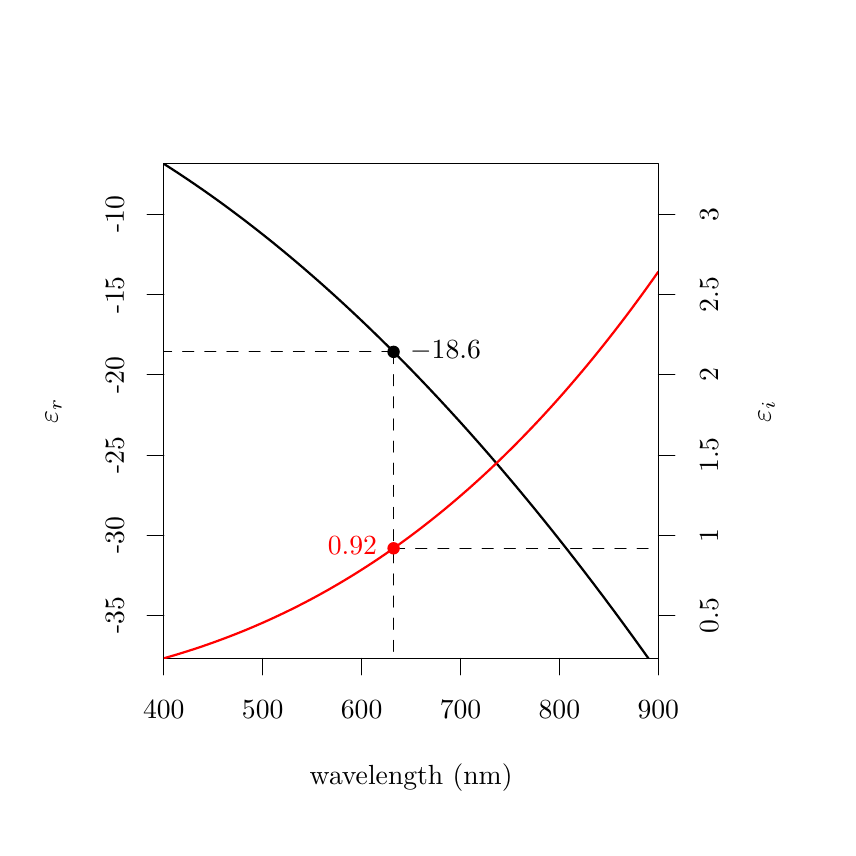
\begin{tikzpicture}[x=1pt,y=1pt]
\definecolor[named]{fillColor}{rgb}{1.00,1.00,1.00}
\path[use as bounding box,fill=fillColor,fill opacity=0.00] (0,0) rectangle (289.08,289.08);
\begin{scope}
\path[clip] (  0.00,  0.00) rectangle (289.08,289.08);
\definecolor[named]{drawColor}{rgb}{0.00,0.00,0.00}

\path[draw=drawColor,line width= 0.4pt,line join=round,line cap=round] ( 49.20, 61.20) -- (227.88, 61.20);

\path[draw=drawColor,line width= 0.4pt,line join=round,line cap=round] ( 49.20, 61.20) -- ( 49.20, 55.20);

\path[draw=drawColor,line width= 0.4pt,line join=round,line cap=round] ( 84.94, 61.20) -- ( 84.94, 55.20);

\path[draw=drawColor,line width= 0.4pt,line join=round,line cap=round] (120.67, 61.20) -- (120.67, 55.20);

\path[draw=drawColor,line width= 0.4pt,line join=round,line cap=round] (156.41, 61.20) -- (156.41, 55.20);

\path[draw=drawColor,line width= 0.4pt,line join=round,line cap=round] (192.14, 61.20) -- (192.14, 55.20);

\path[draw=drawColor,line width= 0.4pt,line join=round,line cap=round] (227.88, 61.20) -- (227.88, 55.20);

\node[text=drawColor,anchor=base,inner sep=0pt, outer sep=0pt, scale=  1.00] at ( 49.20, 39.60) {400};

\node[text=drawColor,anchor=base,inner sep=0pt, outer sep=0pt, scale=  1.00] at ( 84.94, 39.60) {500};

\node[text=drawColor,anchor=base,inner sep=0pt, outer sep=0pt, scale=  1.00] at (120.67, 39.60) {600};

\node[text=drawColor,anchor=base,inner sep=0pt, outer sep=0pt, scale=  1.00] at (156.41, 39.60) {700};

\node[text=drawColor,anchor=base,inner sep=0pt, outer sep=0pt, scale=  1.00] at (192.14, 39.60) {800};

\node[text=drawColor,anchor=base,inner sep=0pt, outer sep=0pt, scale=  1.00] at (227.88, 39.60) {900};

\path[draw=drawColor,line width= 0.4pt,line join=round,line cap=round] ( 49.20, 76.68) -- ( 49.20,221.56);

\path[draw=drawColor,line width= 0.4pt,line join=round,line cap=round] ( 49.20, 76.68) -- ( 43.20, 76.68);

\path[draw=drawColor,line width= 0.4pt,line join=round,line cap=round] ( 49.20,105.66) -- ( 43.20,105.66);

\path[draw=drawColor,line width= 0.4pt,line join=round,line cap=round] ( 49.20,134.63) -- ( 43.20,134.63);

\path[draw=drawColor,line width= 0.4pt,line join=round,line cap=round] ( 49.20,163.61) -- ( 43.20,163.61);

\path[draw=drawColor,line width= 0.4pt,line join=round,line cap=round] ( 49.20,192.59) -- ( 43.20,192.59);

\path[draw=drawColor,line width= 0.4pt,line join=round,line cap=round] ( 49.20,221.56) -- ( 43.20,221.56);

\node[text=drawColor,rotate= 90.00,anchor=base,inner sep=0pt, outer sep=0pt, scale=  1.00] at ( 34.80, 76.68) {-35};

\node[text=drawColor,rotate= 90.00,anchor=base,inner sep=0pt, outer sep=0pt, scale=  1.00] at ( 34.80,105.66) {-30};

\node[text=drawColor,rotate= 90.00,anchor=base,inner sep=0pt, outer sep=0pt, scale=  1.00] at ( 34.80,134.63) {-25};

\node[text=drawColor,rotate= 90.00,anchor=base,inner sep=0pt, outer sep=0pt, scale=  1.00] at ( 34.80,163.61) {-20};

\node[text=drawColor,rotate= 90.00,anchor=base,inner sep=0pt, outer sep=0pt, scale=  1.00] at ( 34.80,192.59) {-15};

\node[text=drawColor,rotate= 90.00,anchor=base,inner sep=0pt, outer sep=0pt, scale=  1.00] at ( 34.80,221.56) {-10};

\path[draw=drawColor,line width= 0.4pt,line join=round,line cap=round] ( 49.20, 61.20) --
	(227.88, 61.20) --
	(227.88,239.88) --
	( 49.20,239.88) --
	( 49.20, 61.20);
\end{scope}
\begin{scope}
\path[clip] ( 49.20, 61.20) rectangle (227.88,239.88);
\definecolor[named]{drawColor}{rgb}{0.00,0.00,0.00}

\path[draw=drawColor,line width= 0.8pt,line join=round,line cap=round] ( 49.20,239.88) --
	( 51.00,238.73) --
	( 52.81,237.56) --
	( 54.61,236.38) --
	( 56.42,235.18) --
	( 58.22,233.97) --
	( 60.03,232.74) --
	( 61.83,231.50) --
	( 63.64,230.25) --
	( 65.44,228.98) --
	( 67.25,227.70) --
	( 69.05,226.40) --
	( 70.86,225.09) --
	( 72.66,223.76) --
	( 74.47,222.42) --
	( 76.27,221.06) --
	( 78.08,219.70) --
	( 79.88,218.31) --
	( 81.69,216.91) --
	( 83.49,215.50) --
	( 85.30,214.07) --
	( 87.10,212.63) --
	( 88.91,211.18) --
	( 90.71,209.71) --
	( 92.52,208.22) --
	( 94.32,206.72) --
	( 96.13,205.21) --
	( 97.93,203.68) --
	( 99.74,202.14) --
	(101.54,200.58) --
	(103.35,199.01) --
	(105.15,197.43) --
	(106.96,195.83) --
	(108.76,194.21) --
	(110.56,192.59) --
	(112.37,190.94) --
	(114.17,189.29) --
	(115.98,187.61) --
	(117.78,185.93) --
	(119.59,184.23) --
	(121.39,182.52) --
	(123.20,180.79) --
	(125.00,179.04) --
	(126.81,177.29) --
	(128.61,175.52) --
	(130.42,173.73) --
	(132.22,171.93) --
	(134.03,170.11) --
	(135.83,168.29) --
	(137.64,166.44) --
	(139.44,164.59) --
	(141.25,162.71) --
	(143.05,160.83) --
	(144.86,158.93) --
	(146.66,157.01) --
	(148.47,155.09) --
	(150.27,153.14) --
	(152.08,151.18) --
	(153.88,149.21) --
	(155.69,147.23) --
	(157.49,145.23) --
	(159.30,143.21) --
	(161.10,141.18) --
	(162.91,139.14) --
	(164.71,137.08) --
	(166.52,135.01) --
	(168.32,132.93) --
	(170.12,130.83) --
	(171.93,128.71) --
	(173.73,126.58) --
	(175.54,124.44) --
	(177.34,122.29) --
	(179.15,120.11) --
	(180.95,117.93) --
	(182.76,115.73) --
	(184.56,113.52) --
	(186.37,111.29) --
	(188.17,109.05) --
	(189.98,106.79) --
	(191.78,104.52) --
	(193.59,102.23) --
	(195.39, 99.94) --
	(197.20, 97.62) --
	(199.00, 95.30) --
	(200.81, 92.95) --
	(202.61, 90.60) --
	(204.42, 88.23) --
	(206.22, 85.84) --
	(208.03, 83.45) --
	(209.83, 81.03) --
	(211.64, 78.61) --
	(213.44, 76.17) --
	(215.25, 73.71) --
	(217.05, 71.24) --
	(218.86, 68.76) --
	(220.66, 66.26) --
	(222.47, 63.75) --
	(224.27, 61.23) --
	(226.08, 58.69) --
	(227.88, 56.13);
\definecolor[named]{drawColor}{rgb}{1.00,0.00,0.00}

\path[draw=drawColor,line width= 0.8pt,line join=round,line cap=round] ( 49.20, 61.20) --
	( 51.00, 61.72) --
	( 52.81, 62.25) --
	( 54.61, 62.79) --
	( 56.42, 63.35) --
	( 58.22, 63.92) --
	( 60.03, 64.50) --
	( 61.83, 65.10) --
	( 63.64, 65.71) --
	( 65.44, 66.34) --
	( 67.25, 66.98) --
	( 69.05, 67.64) --
	( 70.86, 68.31) --
	( 72.66, 68.99) --
	( 74.47, 69.69) --
	( 76.27, 70.40) --
	( 78.08, 71.13) --
	( 79.88, 71.88) --
	( 81.69, 72.64) --
	( 83.49, 73.42) --
	( 85.30, 74.21) --
	( 87.10, 75.02) --
	( 88.91, 75.85) --
	( 90.71, 76.69) --
	( 92.52, 77.55) --
	( 94.32, 78.42) --
	( 96.13, 79.31) --
	( 97.93, 80.22) --
	( 99.74, 81.15) --
	(101.54, 82.09) --
	(103.35, 83.05) --
	(105.15, 84.03) --
	(106.96, 85.03) --
	(108.76, 86.04) --
	(110.56, 87.08) --
	(112.37, 88.13) --
	(114.17, 89.20) --
	(115.98, 90.29) --
	(117.78, 91.39) --
	(119.59, 92.52) --
	(121.39, 93.67) --
	(123.20, 94.83) --
	(125.00, 96.02) --
	(126.81, 97.22) --
	(128.61, 98.44) --
	(130.42, 99.69) --
	(132.22,100.95) --
	(134.03,102.24) --
	(135.83,103.54) --
	(137.64,104.87) --
	(139.44,106.21) --
	(141.25,107.58) --
	(143.05,108.97) --
	(144.86,110.38) --
	(146.66,111.81) --
	(148.47,113.26) --
	(150.27,114.73) --
	(152.08,116.23) --
	(153.88,117.75) --
	(155.69,119.29) --
	(157.49,120.85) --
	(159.30,122.43) --
	(161.10,124.04) --
	(162.91,125.67) --
	(164.71,127.32) --
	(166.52,129.00) --
	(168.32,130.70) --
	(170.12,132.42) --
	(171.93,134.17) --
	(173.73,135.94) --
	(175.54,137.74) --
	(177.34,139.55) --
	(179.15,141.40) --
	(180.95,143.27) --
	(182.76,145.16) --
	(184.56,147.07) --
	(186.37,149.01) --
	(188.17,150.98) --
	(189.98,152.97) --
	(191.78,154.99) --
	(193.59,157.03) --
	(195.39,159.10) --
	(197.20,161.20) --
	(199.00,163.32) --
	(200.81,165.46) --
	(202.61,167.63) --
	(204.42,169.83) --
	(206.22,172.06) --
	(208.03,174.31) --
	(209.83,176.59) --
	(211.64,178.90) --
	(213.44,181.23) --
	(215.25,183.59) --
	(217.05,185.98) --
	(218.86,188.40) --
	(220.66,190.84) --
	(222.47,193.31) --
	(224.27,195.81) --
	(226.08,198.34) --
	(227.88,200.90);
\end{scope}
\begin{scope}
\path[clip] (  0.00,  0.00) rectangle (289.08,289.08);
\definecolor[named]{drawColor}{rgb}{0.00,0.00,0.00}

\path[draw=drawColor,line width= 0.4pt,line join=round,line cap=round] (227.88, 76.68) -- (227.88,221.56);

\path[draw=drawColor,line width= 0.4pt,line join=round,line cap=round] (227.88, 76.68) -- (233.88, 76.68);

\path[draw=drawColor,line width= 0.4pt,line join=round,line cap=round] (227.88,105.66) -- (233.88,105.66);

\path[draw=drawColor,line width= 0.4pt,line join=round,line cap=round] (227.88,134.63) -- (233.88,134.63);

\path[draw=drawColor,line width= 0.4pt,line join=round,line cap=round] (227.88,163.61) -- (233.88,163.61);

\path[draw=drawColor,line width= 0.4pt,line join=round,line cap=round] (227.88,192.59) -- (233.88,192.59);

\path[draw=drawColor,line width= 0.4pt,line join=round,line cap=round] (227.88,221.56) -- (233.88,221.56);

\node[text=drawColor,rotate= 90.00,anchor=base,inner sep=0pt, outer sep=0pt, scale=  1.00] at (249.48, 76.68) {0.5};

\node[text=drawColor,rotate= 90.00,anchor=base,inner sep=0pt, outer sep=0pt, scale=  1.00] at (249.48,105.66) {1};

\node[text=drawColor,rotate= 90.00,anchor=base,inner sep=0pt, outer sep=0pt, scale=  1.00] at (249.48,134.63) {1.5};

\node[text=drawColor,rotate= 90.00,anchor=base,inner sep=0pt, outer sep=0pt, scale=  1.00] at (249.48,163.61) {2};

\node[text=drawColor,rotate= 90.00,anchor=base,inner sep=0pt, outer sep=0pt, scale=  1.00] at (249.48,192.59) {2.5};

\node[text=drawColor,rotate= 90.00,anchor=base,inner sep=0pt, outer sep=0pt, scale=  1.00] at (249.48,221.56) {3};
\end{scope}
\begin{scope}
\path[clip] (  0.00,  0.00) rectangle (289.08,289.08);
\definecolor[named]{drawColor}{rgb}{0.00,0.00,0.00}

\node[text=drawColor,anchor=base,inner sep=0pt, outer sep=0pt, scale=  1.00] at (138.54, 15.60) {wavelength (nm)};

\node[text=drawColor,rotate= 90.00,anchor=base,inner sep=0pt, outer sep=0pt, scale=  1.00] at ( 10.80,150.54) {$\varepsilon_r$};
\end{scope}
\begin{scope}
\path[clip] (  0.00,  0.00) rectangle (289.08,289.08);
\definecolor[named]{drawColor}{rgb}{0.00,0.00,0.00}

\node[text=drawColor,rotate= 90.00,anchor=base,inner sep=0pt, outer sep=0pt, scale=  1.00] at (268.47,150.54) {$\varepsilon_i$};
\end{scope}
\begin{scope}
\path[clip] ( 49.20, 61.20) rectangle (227.88,239.88);
\definecolor[named]{drawColor}{rgb}{0.00,0.00,0.00}

\path[draw=drawColor,line width= 0.4pt,dash pattern=on 4pt off 4pt ,line join=round,line cap=round] (132.22, 47.70) --
	(132.22, 54.24) --
	(132.22, 60.78) --
	(132.22, 67.32) --
	(132.22, 73.86) --
	(132.22, 80.39) --
	(132.22, 86.93) --
	(132.22, 93.47) --
	(132.22,100.01) --
	(132.22,106.55) --
	(132.22,113.09) --
	(132.22,119.62) --
	(132.22,126.16) --
	(132.22,132.70) --
	(132.22,139.24) --
	(132.22,145.78) --
	(132.22,152.31) --
	(132.22,158.85) --
	(132.22,165.39) --
	(132.22,171.93);

\path[draw=drawColor,line width= 0.4pt,dash pattern=on 4pt off 4pt ,line join=round,line cap=round] (132.22,100.95) --
	(139.14,100.95) --
	(146.05,100.95) --
	(152.97,100.95) --
	(159.88,100.95) --
	(166.80,100.95) --
	(173.72,100.95) --
	(180.63,100.95) --
	(187.55,100.95) --
	(194.46,100.95) --
	(201.38,100.95) --
	(208.29,100.95) --
	(215.21,100.95) --
	(222.12,100.95) --
	(229.04,100.95) --
	(235.95,100.95) --
	(242.87,100.95) --
	(249.79,100.95) --
	(256.70,100.95) --
	(263.62,100.95);

\path[draw=drawColor,line width= 0.4pt,dash pattern=on 4pt off 4pt ,line join=round,line cap=round] (  0.00,171.93) --
	(  1.40,171.93) --
	( 13.29,171.93) --
	( 25.19,171.93) --
	( 37.08,171.93) --
	( 48.97,171.93) --
	( 60.87,171.93) --
	( 72.76,171.93) --
	( 84.65,171.93) --
	( 96.54,171.93) --
	(108.44,171.93) --
	(120.33,171.93) --
	(132.22,171.93);
\definecolor[named]{fillColor}{rgb}{0.00,0.00,0.00}

\path[fill=fillColor] (132.22,171.93) circle (  2.25);
\definecolor[named]{fillColor}{rgb}{1.00,0.00,0.00}

\path[fill=fillColor] (132.22,100.95) circle (  2.25);

\node[text=drawColor,anchor=base west,inner sep=0pt, outer sep=0pt, scale=  1.00] at (138.22,169.63) {$-18.6$};
\definecolor[named]{drawColor}{rgb}{1.00,0.00,0.00}

\node[text=drawColor,anchor=base east,inner sep=0pt, outer sep=0pt, scale=  1.00] at (126.22, 98.66) {$0.92$};
\end{scope}
\end{tikzpicture}

\caption[The Drude model for silver calculated with $\omega_p=1.32\times 10^{16}\:\hertz, \gamma=1.4\times 10^{14}\:\hertz$.]{\label{fig:drude}The Drude model calculated with $\omega_p=1.32\times 10^{16}\:\hertz, \gamma=1.4\times 10^{14}\:\hertz$. As an example, the wavelength for a HeNe laser (632.8 nm) is highlighted, showing the permittivity of silver at this wavelength to be $\varepsilon(632.8$ nm$) \approx -18.6+0.92i$}.
\end{center}
\end{figure}
This negative permittivity of metals in the visible domain, when bounded by a dielectric with a positive real permittivity, satisfies the boundary conditions (equation \ref{eq:d-continuous}) for a surface plasmon polariton. Substituting \ref{eq:drude} in to the dispersion relation for a surface plasmon polariton  (equation \ref{eq:spp-dispersion}), we obtain a fair approximation of the dispersion relation for a surface plasmon polariton on a planar metal film. This is plotted in figure \ref{fig:spp-dispersion}.
\begin{figure}
\begin{center}
% Created by tikzDevice version 0.6.2-92-0ad2792 on 2012-09-26 20:23:29
% !TEX encoding = UTF-8 Unicode
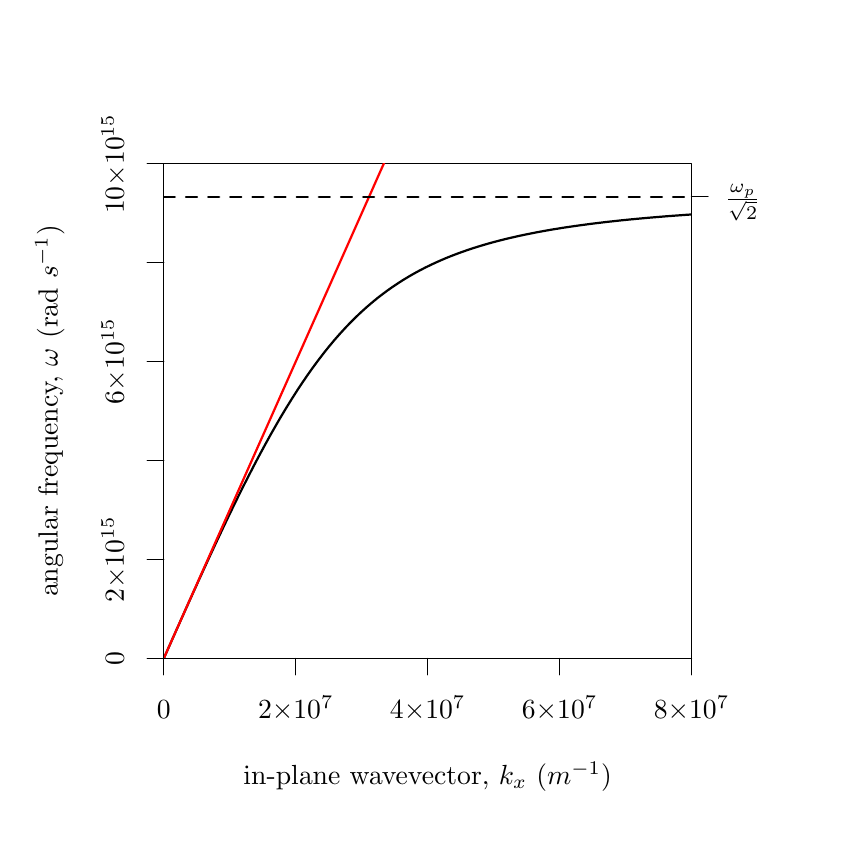
\begin{tikzpicture}[x=1pt,y=1pt]
\definecolor[named]{fillColor}{rgb}{1.00,1.00,1.00}
\path[use as bounding box,fill=fillColor,fill opacity=0.00] (0,0) rectangle (289.08,289.08);
\begin{scope}
\path[clip] (  0.00,  0.00) rectangle (289.08,289.08);
\definecolor[named]{drawColor}{rgb}{0.00,0.00,0.00}

\path[draw=drawColor,line width= 0.4pt,line join=round,line cap=round] ( 49.20, 61.20) --
	(239.88, 61.20) --
	(239.88,239.88) --
	( 49.20,239.88) --
	( 49.20, 61.20);
\end{scope}
\begin{scope}
\path[clip] (  0.00,  0.00) rectangle (289.08,289.08);
\definecolor[named]{drawColor}{rgb}{0.00,0.00,0.00}

\node[text=drawColor,anchor=base,inner sep=0pt, outer sep=0pt, scale=  1.00] at (144.54, 15.60) {in-plane wavevector, $k_x$ ($m^{-1}$)};

\node[text=drawColor,rotate= 90.00,anchor=base,inner sep=0pt, outer sep=0pt, scale=  1.00] at ( 10.80,150.54) {angular frequency, $\omega$ (rad $s^{-1}$)};
\end{scope}
\begin{scope}
\path[clip] ( 49.20, 61.20) rectangle (239.88,239.88);
\definecolor[named]{drawColor}{rgb}{0.00,0.00,0.00}

\path[draw=drawColor,line width= 0.8pt,line join=round,line cap=round] ( 49.20, 61.20) --
	( 51.13, 65.53) --
	( 53.05, 69.86) --
	( 54.98, 74.18) --
	( 56.90, 78.48) --
	( 58.83, 82.77) --
	( 60.76, 87.03) --
	( 62.68, 91.27) --
	( 64.61, 95.48) --
	( 66.53, 99.65) --
	( 68.46,103.78) --
	( 70.39,107.87) --
	( 72.31,111.90) --
	( 74.24,115.89) --
	( 76.16,119.81) --
	( 78.09,123.68) --
	( 80.02,127.47) --
	( 81.94,131.19) --
	( 83.87,134.84) --
	( 85.80,138.40) --
	( 87.72,141.89) --
	( 89.65,145.28) --
	( 91.57,148.59) --
	( 93.50,151.80) --
	( 95.43,154.91) --
	( 97.35,157.93) --
	( 99.28,160.84) --
	(101.20,163.65) --
	(103.13,166.37) --
	(105.06,168.97) --
	(106.98,171.48) --
	(108.91,173.89) --
	(110.83,176.19) --
	(112.76,178.39) --
	(114.69,180.50) --
	(116.61,182.51) --
	(118.54,184.43) --
	(120.46,186.26) --
	(122.39,188.00) --
	(124.32,189.66) --
	(126.24,191.24) --
	(128.17,192.74) --
	(130.09,194.16) --
	(132.02,195.52) --
	(133.95,196.80) --
	(135.87,198.03) --
	(137.80,199.19) --
	(139.72,200.29) --
	(141.65,201.34) --
	(143.58,202.34) --
	(145.50,203.28) --
	(147.43,204.18) --
	(149.36,205.04) --
	(151.28,205.86) --
	(153.21,206.63) --
	(155.13,207.37) --
	(157.06,208.07) --
	(158.99,208.74) --
	(160.91,209.38) --
	(162.84,209.99) --
	(164.76,210.57) --
	(166.69,211.13) --
	(168.62,211.66) --
	(170.54,212.16) --
	(172.47,212.65) --
	(174.39,213.11) --
	(176.32,213.55) --
	(178.25,213.98) --
	(180.17,214.38) --
	(182.10,214.77) --
	(184.02,215.15) --
	(185.95,215.50) --
	(187.88,215.85) --
	(189.80,216.18) --
	(191.73,216.49) --
	(193.65,216.80) --
	(195.58,217.09) --
	(197.51,217.37) --
	(199.43,217.64) --
	(201.36,217.90) --
	(203.28,218.16) --
	(205.21,218.40) --
	(207.14,218.63) --
	(209.06,218.86) --
	(210.99,219.07) --
	(212.92,219.28) --
	(214.84,219.49) --
	(216.77,219.68) --
	(218.69,219.87) --
	(220.62,220.05) --
	(222.55,220.23) --
	(224.47,220.40) --
	(226.40,220.56) --
	(228.32,220.72) --
	(230.25,220.88) --
	(232.18,221.03) --
	(234.10,221.17) --
	(236.03,221.31) --
	(237.95,221.45) --
	(239.88,221.58);
\definecolor[named]{drawColor}{rgb}{1.00,0.00,0.00}

\path[draw=drawColor,line width= 0.8pt,line join=round,line cap=round] ( 49.20, 61.20) --
	( 51.13, 65.53) --
	( 53.05, 69.86) --
	( 54.98, 74.19) --
	( 56.90, 78.53) --
	( 58.83, 82.86) --
	( 60.76, 87.19) --
	( 62.68, 91.52) --
	( 64.61, 95.85) --
	( 66.53,100.18) --
	( 68.46,104.52) --
	( 70.39,108.85) --
	( 72.31,113.18) --
	( 74.24,117.51) --
	( 76.16,121.84) --
	( 78.09,126.17) --
	( 80.02,130.51) --
	( 81.94,134.84) --
	( 83.87,139.17) --
	( 85.80,143.50) --
	( 87.72,147.83) --
	( 89.65,152.16) --
	( 91.57,156.50) --
	( 93.50,160.83) --
	( 95.43,165.16) --
	( 97.35,169.49) --
	( 99.28,173.82) --
	(101.20,178.15) --
	(103.13,182.49) --
	(105.06,186.82) --
	(106.98,191.15) --
	(108.91,195.48) --
	(110.83,199.81) --
	(112.76,204.14) --
	(114.69,208.48) --
	(116.61,212.81) --
	(118.54,217.14) --
	(120.46,221.47) --
	(122.39,225.80) --
	(124.32,230.13) --
	(126.24,234.47) --
	(128.17,238.80) --
	(130.09,243.13) --
	(132.02,247.46) --
	(133.95,251.79) --
	(135.87,256.12) --
	(137.80,260.46) --
	(139.72,264.79) --
	(141.65,269.12) --
	(143.58,273.45) --
	(145.50,277.78) --
	(147.43,282.11) --
	(149.36,286.45) --
	(150.53,289.08);
\definecolor[named]{drawColor}{rgb}{0.00,0.00,0.00}

\path[draw=drawColor,line width= 0.8pt,dash pattern=on 4pt off 4pt ,line join=round,line cap=round] ( 49.20,227.98) --
	( 51.13,227.98) --
	( 53.05,227.98) --
	( 54.98,227.98) --
	( 56.90,227.98) --
	( 58.83,227.98) --
	( 60.76,227.98) --
	( 62.68,227.98) --
	( 64.61,227.98) --
	( 66.53,227.98) --
	( 68.46,227.98) --
	( 70.39,227.98) --
	( 72.31,227.98) --
	( 74.24,227.98) --
	( 76.16,227.98) --
	( 78.09,227.98) --
	( 80.02,227.98) --
	( 81.94,227.98) --
	( 83.87,227.98) --
	( 85.80,227.98) --
	( 87.72,227.98) --
	( 89.65,227.98) --
	( 91.57,227.98) --
	( 93.50,227.98) --
	( 95.43,227.98) --
	( 97.35,227.98) --
	( 99.28,227.98) --
	(101.20,227.98) --
	(103.13,227.98) --
	(105.06,227.98) --
	(106.98,227.98) --
	(108.91,227.98) --
	(110.83,227.98) --
	(112.76,227.98) --
	(114.69,227.98) --
	(116.61,227.98) --
	(118.54,227.98) --
	(120.46,227.98) --
	(122.39,227.98) --
	(124.32,227.98) --
	(126.24,227.98) --
	(128.17,227.98) --
	(130.09,227.98) --
	(132.02,227.98) --
	(133.95,227.98) --
	(135.87,227.98) --
	(137.80,227.98) --
	(139.72,227.98) --
	(141.65,227.98) --
	(143.58,227.98) --
	(145.50,227.98) --
	(147.43,227.98) --
	(149.36,227.98) --
	(151.28,227.98) --
	(153.21,227.98) --
	(155.13,227.98) --
	(157.06,227.98) --
	(158.99,227.98) --
	(160.91,227.98) --
	(162.84,227.98) --
	(164.76,227.98) --
	(166.69,227.98) --
	(168.62,227.98) --
	(170.54,227.98) --
	(172.47,227.98) --
	(174.39,227.98) --
	(176.32,227.98) --
	(178.25,227.98) --
	(180.17,227.98) --
	(182.10,227.98) --
	(184.02,227.98) --
	(185.95,227.98) --
	(187.88,227.98) --
	(189.80,227.98) --
	(191.73,227.98) --
	(193.65,227.98) --
	(195.58,227.98) --
	(197.51,227.98) --
	(199.43,227.98) --
	(201.36,227.98) --
	(203.28,227.98) --
	(205.21,227.98) --
	(207.14,227.98) --
	(209.06,227.98) --
	(210.99,227.98) --
	(212.92,227.98) --
	(214.84,227.98) --
	(216.77,227.98) --
	(218.69,227.98) --
	(220.62,227.98) --
	(222.55,227.98) --
	(224.47,227.98) --
	(226.40,227.98) --
	(228.32,227.98) --
	(230.25,227.98) --
	(232.18,227.98) --
	(234.10,227.98) --
	(236.03,227.98) --
	(237.95,227.98) --
	(239.88,227.98);
\end{scope}
\begin{scope}
\path[clip] (  0.00,  0.00) rectangle (289.08,289.08);
\definecolor[named]{drawColor}{rgb}{0.00,0.00,0.00}

\path[draw=drawColor,line width= 0.4pt,line join=round,line cap=round] ( 49.20, 61.20) -- (239.88, 61.20);

\path[draw=drawColor,line width= 0.4pt,line join=round,line cap=round] ( 49.20, 61.20) -- ( 49.20, 55.20);

\path[draw=drawColor,line width= 0.4pt,line join=round,line cap=round] ( 96.87, 61.20) -- ( 96.87, 55.20);

\path[draw=drawColor,line width= 0.4pt,line join=round,line cap=round] (144.54, 61.20) -- (144.54, 55.20);

\path[draw=drawColor,line width= 0.4pt,line join=round,line cap=round] (192.21, 61.20) -- (192.21, 55.20);

\path[draw=drawColor,line width= 0.4pt,line join=round,line cap=round] (239.88, 61.20) -- (239.88, 55.20);

\node[text=drawColor,anchor=base,inner sep=0pt, outer sep=0pt, scale=  1.00] at ( 49.20, 39.60) {0};

\node[text=drawColor,anchor=base,inner sep=0pt, outer sep=0pt, scale=  1.00] at ( 96.87, 39.60) {2$\times 10^7$};

\node[text=drawColor,anchor=base,inner sep=0pt, outer sep=0pt, scale=  1.00] at (144.54, 39.60) {4$\times 10^7$};

\node[text=drawColor,anchor=base,inner sep=0pt, outer sep=0pt, scale=  1.00] at (192.21, 39.60) {6$\times 10^7$};

\node[text=drawColor,anchor=base,inner sep=0pt, outer sep=0pt, scale=  1.00] at (239.88, 39.60) {8$\times 10^7$};

\path[draw=drawColor,line width= 0.4pt,line join=round,line cap=round] ( 49.20, 61.20) -- ( 49.20,239.88);

\path[draw=drawColor,line width= 0.4pt,line join=round,line cap=round] ( 49.20, 61.20) -- ( 43.20, 61.20);

\path[draw=drawColor,line width= 0.4pt,line join=round,line cap=round] ( 49.20, 96.94) -- ( 43.20, 96.94);

\path[draw=drawColor,line width= 0.4pt,line join=round,line cap=round] ( 49.20,132.67) -- ( 43.20,132.67);

\path[draw=drawColor,line width= 0.4pt,line join=round,line cap=round] ( 49.20,168.41) -- ( 43.20,168.41);

\path[draw=drawColor,line width= 0.4pt,line join=round,line cap=round] ( 49.20,204.14) -- ( 43.20,204.14);

\path[draw=drawColor,line width= 0.4pt,line join=round,line cap=round] ( 49.20,239.88) -- ( 43.20,239.88);

\node[text=drawColor,rotate= 90.00,anchor=base,inner sep=0pt, outer sep=0pt, scale=  1.00] at ( 34.80, 61.20) {0};

\node[text=drawColor,rotate= 90.00,anchor=base,inner sep=0pt, outer sep=0pt, scale=  1.00] at ( 34.80, 96.94) {2$\times 10^{15}$};

\node[text=drawColor,rotate= 90.00,anchor=base,inner sep=0pt, outer sep=0pt, scale=  1.00] at ( 34.80,168.41) {6$\times 10^{15}$};

\node[text=drawColor,rotate= 90.00,anchor=base,inner sep=0pt, outer sep=0pt, scale=  1.00] at ( 34.80,239.88) {10$\times 10^{15}$};

\path[draw=drawColor,line width= 0.4pt,line join=round,line cap=round] (239.88,227.98) -- (239.88,227.98);

\path[draw=drawColor,line width= 0.4pt,line join=round,line cap=round] (239.88,227.98) -- (245.88,227.98);

\node[text=drawColor,anchor=base west,inner sep=0pt, outer sep=0pt, scale=  1.00] at (251.88,224.53) {$\frac{\omega_p}{\sqrt{2}}$};
\end{scope}
\end{tikzpicture}

\caption[The dispersion of a surface plasmon polariton on a planar film approximated with the Drude mode.]{\label{fig:spp-dispersion}The dispersion of a surface plasmon polariton on a planar film approximated with the Drude model with $\omega_p=1.32\times 10^{16}\:\hertz, \gamma=1.4\times 10^{14} \:\hertz$.}
\end{center}
\end{figure}
Figure \ref{fig:spp-dispersion} shows the dispersion of a surface plasmon polariton on a flat interface between silver and air. Plotted on the same scale is a line representing a grazing photon along the surface, the `light-line'.  Notice that the light line and the surface plasmon polariton dispersion line do not cross. There is no solution at which the energy and momentum of free-space light is equal to that of the surface plasmon polariton. Since for a given energy of light, the light possesses insufficient momentum to match that of an SPP, the conclusion is that free-space light incident on a flat metallic surface cannot resonantly drive a surface plasmon polariton. 


\subsection{Penetration Depth}

An excited SPP at the interface between a conductor and dielectric will possess electromagnetic fields which decay exponentially into both bounding media. A useful measure of this decay is the penetration depth, $L_z$, which is the distance at which the field amplitude has decreased to $1/e$ of it's maximum value.
Momentum conservation for a SPP (where $k_x>\varepsilon_m k_0$) gives an expression $k_{z_m}=\sqrt{\varepsilon_m k_0^2-k_x^2}$ (equation \ref{eq:momentum-conservation} simplified.), which leads to the conclusion that $k_{z_m}$ for SPPs must be purely imaginary. Substituting an imaginary $k_{z_m}$ into an expression for the electric field at the surface gives\footnote{the time dependent term, $e^{-i \omega t}$ has been omitted for clarity.},
\begin{equation}
\mathbf{E}_m = [E_{x_m},0,E_{z_m}]\,e^{i k_{x}x}e^{-k_{z_m} z}
\end{equation}
which is an expression for an electric field which does indeed decay exponentially into the two bounding media, and travels along the surface in the $x$ direction. The value of $z$ for which $E_{z_m}$ falls to $e^{-1}$ of the maximum value is then $1/k_{z_m}$. Substituting equation \ref{eq:dispersion} into equation \ref{eq:momentum-conservation} we find that the expression for $k_{z_m}$ is given by,
\begin{equation}
k_{z_m}=\pm k_0\sqrt{\varepsilon_m - \left(\frac{\varepsilon_1 \varepsilon_2}{\varepsilon_1+\varepsilon_2}\right)}=\pm k_0 \sqrt{ \frac{\varepsilon_m^2}{\varepsilon_1+\varepsilon_2}}\label{eq:kzL}
\end{equation}
We may simplify this expression for the case under consideration with medium $m=1$ being a non-absorbing dielectric, $\operatorname{Re}(\varepsilon_1)>0$ and $\operatorname{Im}(\varepsilon_1)=0$, and medium $m=2$ a lossy metal, $\operatorname{Re}(\varepsilon_2)<0$  and $\operatorname{Im}(\varepsilon_2)>0$. In the case where the metal is highly conducting we also have the considerations $|\operatorname{Re}(\varepsilon_2)|\gg 1$ and $|\operatorname{Re}(\varepsilon_2)|\gg \operatorname{Im}(\varepsilon_2)$. Under these conditions, equation \ref{eq:kzL} simplifies to,
\begin{equation}
k_{z_m}=\pm k_0 \sqrt{\frac{\operatorname{Re}(\varepsilon_m)^2}{\operatorname{Re}(\varepsilon_2)}}
\end{equation}
The penetration depth is then,
\begin{equation}
L_{z_m}=\frac{1}{k_{z_m}}=\lambda_0\:\frac{1}{2\pi}\sqrt{\frac{|\operatorname{Re}(\varepsilon_2)|}{|\operatorname{Re}(\varepsilon_m)^2|}}\label{eq:fieldpenetration}
\end{equation}
For a typical planar silver surface in air with  $k_0=2\pi/\lambda_0=2\pi/632.8\:\nano\metre$, the penetration depth for the SPP into the air is calculated, using equation \ref{eq:fieldpenetration}, to be $L_{z_1}\approx 415\:\nano\metre$ and in to the metal $L_{z_2}\approx 24\:\nano\metre$.
\begin{figure}
\begin{center}
\subfigure[]{\begin{pspicture}[](4,5) %start optics diagram (8x5) grid
	\pnode(4,2){C} %labeled nodes are the positions in the (8x5) grid
	\pnode(0.5,5){i} %labeled nodes are the positions in the (8x5) grid
	\pnode(7.5,5){r} %labeled nodes are the positions in the (8x5) grid
	\pnode(8,0.5){t}
	
	\addtopsstyle{ExtendedMirror}{hatchcolor=lightgray}
	\mirror[mirrorwidth=4,mirrortype=extended,mirrordepth=2](2,5)(2,2)(2,5)
	
\psbezier[ArrowInside=->, arrowscale=2,ArrowInsideOffset=0.01](0,2)(0,5)(2,5)(2,2)
\psbezier[ArrowInside=->, arrowscale=2,ArrowInsideOffset=0.03](0.1,2)(0.1,4)(1.9,4)(1.9,2)
\psbezier[ArrowInside=->, arrowscale=2,ArrowInsideOffset=0.03](0.2,2)(0.2,3)(1.8,3)(1.8,2)

\psbezier[ArrowInside=->, arrowscale=2,ArrowInsideOffset=0.01](4,2)(4,5)(2,5)(2,2)
\psbezier[ArrowInside=->, arrowscale=2,ArrowInsideOffset=0.03](3.9,2)(3.9,4)(2.1,4)(2.1,2)
\psbezier[ArrowInside=->, arrowscale=2,ArrowInsideOffset=0.03](3.8,2)(3.8,3)(2.2,3)(2.2,2)

\psbezier[ArrowInside=->, arrowscale=2,ArrowInsideOffset=0.03](0,2)(0,0.8)(2,0.8)(2,2)
\psbezier[ArrowInside=->, arrowscale=2,ArrowInsideOffset=0.03](0.1,2)(0.1,1.25)(1.9,1.25)(1.9,2)
\psbezier[ArrowInside=->, arrowscale=2,ArrowInsideOffset=0.03](0.2,2)(0.2,1.55)(1.8,1.55)(1.8,2)

\psbezier[ArrowInside=->, arrowscale=2,ArrowInsideOffset=0.03](4,2)(4,0.8)(2,0.8)(2,2)
\psbezier[ArrowInside=->, arrowscale=2,ArrowInsideOffset=0.03](3.9,2)(3.9,1.25)(2.1,1.25)(2.1,2)
\psbezier[ArrowInside=->, arrowscale=2,ArrowInsideOffset=0.03](3.8,2)(3.8,1.55)(2.2,1.55)(2.2,2)

\rput(0.5,0.25){$\varepsilon_2$}
\rput(0.5,4.75){$\varepsilon_1$}
\rput(2.5, 4.5){$\mathbf{E}$}
\rput[Cl](0,1.95){\red $\mathbf{+ +}$}
\rput[Cr](4,1.95){\red $\mathbf{+ +}$}
\rput(2,1.95){\blue $\mathbf{- -}$}



\end{pspicture}}
\subfigure[]{\begin{pspicture}[](4,5) %start optics diagram (8x5) grid
	
%	\addtopsstyle{ExtendedMirror}{hatchcolor=lightgray}
%	\mirror[mirrorwidth=4,mirrortype=extended,mirrordepth=2](2,5)(2,2)(2,5)
	
\rput(3,1.5){$\varepsilon_2$}
\rput(3,2.5){$\varepsilon_1$}
\rput(4, 2){$\lvert\mathbf{E}_z\rvert$}
\psline[linewidth=0.05]{->}(0,2)(3.5,2)
\psline[linewidth=0.05]{<->}(0,0)(0,4.75)
\psbezier[linecolor=red](0.1,4.75)(0.1,2)(3,2)(3,2)
\psbezier[linecolor=red](0.1,0)(0.1,2)(0,2)(3,2)
\rput(0,5){z}


\end{pspicture}}
\caption[Diagram of the electric field vectors of a SPP at the interface between a metal and a dielectric and the exponential decay of the $E_z$ component away from the surface.]{(a) Diagram of the electric field vectors of a SPP at the interface between a metal and a dielectric. (b) The exponential decay of the $E_z$ component away from the surface, with a maximum amplitude at $z=0$ and the different penetration lengths for the two materials shown. \label{fig:fieldlinescartoon}}
\end{center}
\end{figure}
The field at the surface and this associated exponential decay of the SPP fields in the $z$ direction is shown diagrammatically in figure \ref{fig:fieldlinescartoon} for an SPP in the visible regime. 

In the limit of a perfect conductor, where $\varepsilon_2 \rightarrow -\infty$, equation \ref{eq:fieldpenetration} shows that the penetration depth into the metal $L_{z_1}\rightarrow 0$ and the penetration depth into the dielectric tends to $L_{z_2}\rightarrow \infty$. With no field in the metal and the `decay length' in $z$ never actually decaying in the dielectric medium, the result is a grazing plane wave and no localisation of the field to the surface can be said to exist. This is why the excitation of SPP waves in the microwave regime is not observed on unaltered planar surfaces, as at these frequencies the metals approximate a perfect conductor and so the vanishingly-small localisation of the bound surface modes leads to the SPP resembling a grazing photon. 


\subsection{Propagation Length}
By similar considerations of the surface electric field, we define the propagation length of the SPP along the surface as the length at which the field intensity has fallen to $e^{-1}$ of its maximum value. While the SPP propagates in the $x$ direction, it will be damped by Joule losses to the metal. This leads to the expression for $k_x$ to be generally complex, and the imaginary component of of $k_x$ again provides the exponential decay of the SPP as it travels along the interface. The imaginary part of $k_x$ is given by,
\begin{equation}
\operatorname{Im}(k_x)=\frac{k_0 \operatorname{Im}(\varepsilon_2)}{2\operatorname{Re}(\varepsilon_2)^2}\left(\frac{\varepsilon_1\operatorname{Re}(\varepsilon_2)}{\varepsilon_1+\operatorname{Re}(\varepsilon_2)}\right)^{\frac{3}{2}}
\end{equation} 
This gives the propagation length, $L_x$ as,
\begin{equation}
L_x=\lambda_0\:\frac{\operatorname{Re}(\varepsilon_2)^2}{2 \pi \operatorname{Im}(\varepsilon_2)}\left(\frac{\varepsilon_1+\operatorname{Re}(\varepsilon_2)}{\varepsilon_1\operatorname{Re}(\varepsilon_2)}\right)^{\frac{3}{2}}
\end{equation}
For a typical planar silver surface in air with  $k_0=2\pi/\lambda_0=2\pi/632.8\:\nano\metre$, the propagation length is $L_x=42.6\:\micro\metre$. This propagation length is large enough so the SPP intensity is sufficient to interact strongly and Bragg scatter on diffraction  gratings with sub-micron periodicity, a topic we shall cover in the next section.


\section{Surface Plasmon Polaritons on Diffraction Gratings\label{sec:SPPsDG}}
\subsection{Diffraction Gratings}

A diffraction grating is an optical device in which the dielectric constant varies periodically across the surface, and whose period is of the order of the wavelength of light. This periodic variation leads to the diffraction of light by way of localised phase changes in the impinging field, resulting in either the coherent constructive or destructive interference of the waves in the far-field.

The first recorded observation of diffraction by fine structure was by Francis Hopkinson in the late 1700s. Peering at a street lamp through a silk handkerchief, Hopkinson observed rainbows and enquired with his friend, Rittenhause as to the cause. Rittenhause then went on to manufacture and study the first reported `diffraction grating' made of parallel hairs, set between two brass wires cut with a fine screw head \cite{Rittenhause1786}. This was the first example of a transmission grating and the device's dispersive nature.

In this thesis, a periodic modulation across a reflecting surface is achieved by surface-relief. Shallow grooves are cut into a metal surface with a defined period, on the order of the wavelength of visible light, causing diffraction in the reflected light from the surface. Other methods by which diffraction gratings may be produced exist, such as phase-modulated diffraction gratings \cite{Palmer2005} or periodic hole arrays, but these will not be dealt with here.

\begin{figure}
\begin{center}
\input{figure-asimple-coordinate-latexannotations.pdf_tex}
\end{center}
\caption{The coordinate system used for a simple grating in the conical mount.\label{fig:simple-coordsys}}
\end{figure} 

The coordinate system for a simple reflection grating of this type is shown in figure \ref{fig:simple-coordsys}. The grating consists of a set of periodic grooves in a metal surface, with the amplitude varying along the $x$-axis, with a periodicity of $\lambda_{gx}$\nomenclature{$\lambda_{gx}$}{The period of a grating along the $x$-axis.}. Light impinges on the grating surface at a polar angle $\theta$,\nomenclature{$\theta$}{The polar angle of incidence, the angle between the surface normal and the incident light.} in a plane of incidence defined at an azimuthal angle $\phi$\nomenclature{$\phi$}{The azimuthal angle of incidence, defining the orientation of the plane of incidence with respect to the $x$-axis.}, where $\phi=0^\circ$ corresponds to when the plane of incidence is perpendicular to the grating grooves. The grooves are a depth $d$. The polarisation of the incident light is defined with respect to the plane of incidence, such that Transverse Electric (TE) polarised light is when the electric field, $\mathbf{E}_{TE}$ is oriented perpendicular (transverse) to the plane of incidence, and Transverse Magnetic polarised light is defined as the electric vector $\mathbf{E}_{TM}$ lying within the plane of incidence.

In this orientation, where $\phi$ is allowed to vary and is not necessarily equal to $0^\circ$, the diffracted beams form in general a `cone' of diffraction, and so it is named the `conical' mounting/arrangement.
 
The relationship between incident and diffracted light in the conical mount is given by the equation,
\begin{equation}
n\:\frac{\lambda_0}{\lambda_{gx}}=(\sin{\theta}\cos{\phi}+\sin{\theta_n}\cos{\phi_n})\label{eq:gratinequation}
\end{equation}
where $n$ is an integer denoting the spectral order of diffraction, $\lambda_0$ is the incident wavelength and $\theta_n, \phi_n$ is the polar and azimuthal angle of the $n^{th}$ diffracted order, respectively.

The wavevector of light is defined as $\mathbf{k}_0=2\pi\hat{\mathbf{r}}/\lambda_0$, where $\hat{\mathbf{r}}$ is the unit vector denoting the direction of the wave. This wavevector is associated with the light's momentum by a factor of the reduced Planck's constant, such that $\mathbf{p}=\hbar\:\mathbf{k}_0$, and it's scalar equivalent is the wavenumber ($k_0$). Similarly, the grating wavevector is defined, in this case, as $\mathbf{k}_{gx}=2\pi\hat{\mathbf{x}}/\lambda_{gx}$\nomenclature{$\mathbf{k}_{gx}$}{The grating wavevector for the diffraction grating varying along the $x$ axis.} (its wavenumber is $k_{gx}$). We may re-write equation \ref{eq:gratinequation} in terms of these quantities,
\begin{align}
-k_0\sin{\theta_n}\cos{\phi_n}&=k_0 \sin{\theta}\cos{\phi}-n k_{gx}\\
\mathbf{k}_n^\parallel&=\mathbf{k}_0^\parallel-n \mathbf{k}_{gx}\label{eq:addgratinvector}
\end{align}
where $\mathbf{k}_n^\parallel$ is the wavevector component of the diffracted light parallel to the surface and $\mathbf{k}_0^\parallel$ is the incident light's wavevector parallel to the surface.
So a diffraction grating modifies the surface wavevector of the incident light  by the addition or subtraction (since $n$ may be positive or negative) of an integer number of grating wavevectors. 

Recall from section \ref{sec:SPPs} that the coupling of free-space light to surface plasmon polaritons is not possible on flat surfaces due to the mismatch between the SPP and light's wavevectors (or, equivalently, the momentum mismatch). Since the diffraction grating allows us to modify the wavevector of incident light, the diffraction grating may be used to couple to these previously unmatchable modes. This will be explored in the next subsection.

\subsection{Coupling Surface Plasmons to Light by Coherent Scattering}
\begin{figure}
\begin{center}
\subfigure[]{% Created by tikzDevice version 0.6.2-92-0ad2792 on 2012-09-24 19:13:05
% !TEX encoding = UTF-8 Unicode
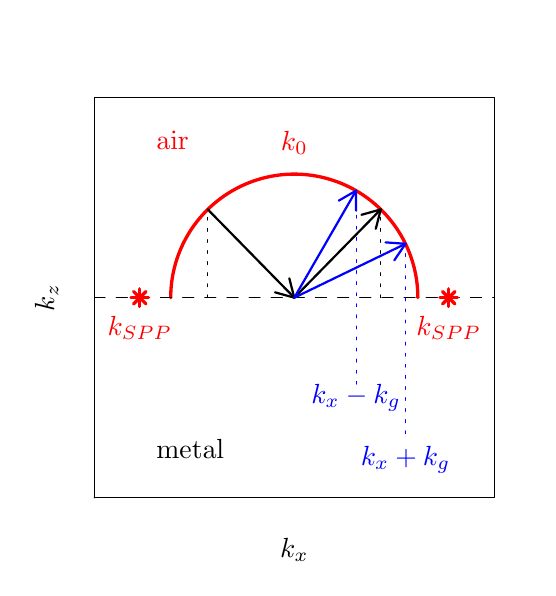
\begin{tikzpicture}[x=1pt,y=1pt]
\definecolor[named]{fillColor}{rgb}{1.00,1.00,1.00}
\path[use as bounding box,fill=fillColor,fill opacity=0.00] (0,0) rectangle (180.67,195.13);
\begin{scope}
\path[clip] (  0.00,  0.00) rectangle (180.67,195.13);
\definecolor[named]{drawColor}{rgb}{0.00,0.00,0.00}

\path[draw=drawColor,line width= 0.4pt,line join=round,line cap=round] ( 24.00, 25.23) --
	(168.67, 25.23) --
	(168.67,169.90) --
	( 24.00,169.90) --
	( 24.00, 25.23);

\node[text=drawColor,anchor=base,inner sep=0pt, outer sep=0pt, scale=  1.00] at ( 96.34,  3.63) {$k_x$};

\node[text=drawColor,rotate= 90.00,anchor=base,inner sep=0pt, outer sep=0pt, scale=  1.00] at (  9.60, 97.56) {$k_z$};
\end{scope}
\begin{scope}
\path[clip] ( 24.00, 25.23) rectangle (168.67,169.90);
\definecolor[named]{drawColor}{rgb}{1.00,0.00,0.00}

\path[draw=drawColor,line width= 1.2pt,line join=round,line cap=round] (140.99, 97.56) --
	(140.97, 98.98) --
	(140.90,100.40) --
	(140.79,101.81) --
	(140.63,103.22) --
	(140.43,104.62) --
	(140.18,106.02) --
	(139.89,107.40) --
	(139.56,108.78) --
	(139.18,110.14) --
	(138.76,111.50) --
	(138.30,112.84) --
	(137.79,114.16) --
	(137.24,115.47) --
	(136.66,116.76) --
	(136.03,118.03) --
	(135.36,119.27) --
	(134.65,120.50) --
	(133.90,121.71) --
	(133.12,122.89) --
	(132.30,124.04) --
	(131.44,125.17) --
	(130.54,126.27) --
	(129.62,127.34) --
	(128.65,128.38) --
	(127.66,129.39) --
	(126.63,130.37) --
	(125.58,131.31) --
	(124.49,132.22) --
	(123.38,133.10) --
	(122.24,133.94) --
	(121.07,134.74) --
	(119.88,135.51) --
	(118.66,136.23) --
	(117.43,136.92) --
	(116.17,137.57) --
	(114.89,138.18) --
	(113.59,138.75) --
	(112.27,139.28) --
	(110.94,139.76) --
	(109.60,140.20) --
	(108.24,140.60) --
	(106.86,140.96) --
	(105.48,141.27) --
	(104.09,141.54) --
	(102.69,141.76) --
	(101.29,141.94) --
	( 99.88,142.08) --
	( 98.46,142.17) --
	( 97.05,142.21) --
	( 95.63,142.21) --
	( 94.21,142.17) --
	( 92.80,142.08) --
	( 91.39,141.94) --
	( 89.98,141.76) --
	( 88.58,141.54) --
	( 87.19,141.27) --
	( 85.81,140.96) --
	( 84.44,140.60) --
	( 83.08,140.20) --
	( 81.73,139.76) --
	( 80.40,139.28) --
	( 79.09,138.75) --
	( 77.79,138.18) --
	( 76.51,137.57) --
	( 75.25,136.92) --
	( 74.01,136.23) --
	( 72.80,135.51) --
	( 71.60,134.74) --
	( 70.44,133.94) --
	( 69.30,133.10) --
	( 68.18,132.22) --
	( 67.10,131.31) --
	( 66.04,130.37) --
	( 65.01,129.39) --
	( 64.02,128.38) --
	( 63.06,127.34) --
	( 62.13,126.27) --
	( 61.24,125.17) --
	( 60.38,124.04) --
	( 59.56,122.89) --
	( 58.77,121.71) --
	( 58.03,120.50) --
	( 57.32,119.27) --
	( 56.65,118.03) --
	( 56.02,116.76) --
	( 55.43,115.47) --
	( 54.88,114.16) --
	( 54.38,112.84) --
	( 53.91,111.50) --
	( 53.49,110.14) --
	( 53.12,108.78) --
	( 52.78,107.40) --
	( 52.49,106.02) --
	( 52.25,104.62) --
	( 52.04,103.22) --
	( 51.89,101.81) --
	( 51.77,100.40) --
	( 51.71, 98.98) --
	( 51.68, 97.56);
\definecolor[named]{drawColor}{rgb}{0.00,0.00,0.00}

\path[draw=drawColor,line width= 0.4pt,dash pattern=on 4pt off 4pt ,line join=round,line cap=round] (  0.00, 97.56) --
	(  0.27, 97.56) --
	(  2.97, 97.56) --
	(  5.68, 97.56) --
	(  8.39, 97.56) --
	( 11.09, 97.56) --
	( 13.80, 97.56) --
	( 16.50, 97.56) --
	( 19.21, 97.56) --
	( 21.92, 97.56) --
	( 24.62, 97.56) --
	( 27.33, 97.56) --
	( 30.03, 97.56) --
	( 32.74, 97.56) --
	( 35.45, 97.56) --
	( 38.15, 97.56) --
	( 40.86, 97.56) --
	( 43.57, 97.56) --
	( 46.27, 97.56) --
	( 48.98, 97.56) --
	( 51.68, 97.56) --
	( 54.39, 97.56) --
	( 57.10, 97.56) --
	( 59.80, 97.56) --
	( 62.51, 97.56) --
	( 65.22, 97.56) --
	( 67.92, 97.56) --
	( 70.63, 97.56) --
	( 73.33, 97.56) --
	( 76.04, 97.56) --
	( 78.75, 97.56) --
	( 81.45, 97.56) --
	( 84.16, 97.56) --
	( 86.87, 97.56) --
	( 89.57, 97.56) --
	( 92.28, 97.56) --
	( 94.98, 97.56) --
	( 97.69, 97.56) --
	(100.40, 97.56) --
	(103.10, 97.56) --
	(105.81, 97.56) --
	(108.52, 97.56) --
	(111.22, 97.56) --
	(113.93, 97.56) --
	(116.63, 97.56) --
	(119.34, 97.56) --
	(122.05, 97.56) --
	(124.75, 97.56) --
	(127.46, 97.56) --
	(130.17, 97.56) --
	(132.87, 97.56) --
	(135.58, 97.56) --
	(138.28, 97.56) --
	(140.99, 97.56) --
	(143.70, 97.56) --
	(146.40, 97.56) --
	(149.11, 97.56) --
	(151.82, 97.56) --
	(154.52, 97.56) --
	(157.23, 97.56) --
	(159.93, 97.56) --
	(162.64, 97.56) --
	(165.35, 97.56) --
	(168.05, 97.56) --
	(170.76, 97.56) --
	(173.47, 97.56) --
	(176.17, 97.56) --
	(178.88, 97.56) --
	(180.67, 97.56);
\definecolor[named]{drawColor}{rgb}{1.00,0.00,0.00}

\path[draw=drawColor,line width= 1.2pt,line join=round,line cap=round] ( 38.27, 95.31) -- ( 42.77, 99.81);

\path[draw=drawColor,line width= 1.2pt,line join=round,line cap=round] ( 38.27, 99.81) -- ( 42.77, 95.31);

\path[draw=drawColor,line width= 1.2pt,line join=round,line cap=round] ( 37.34, 97.56) -- ( 43.70, 97.56);

\path[draw=drawColor,line width= 1.2pt,line join=round,line cap=round] ( 40.52, 94.38) -- ( 40.52,100.75);

\path[draw=drawColor,line width= 1.2pt,line join=round,line cap=round] (149.90, 95.31) -- (154.40, 99.81);

\path[draw=drawColor,line width= 1.2pt,line join=round,line cap=round] (149.90, 99.81) -- (154.40, 95.31);

\path[draw=drawColor,line width= 1.2pt,line join=round,line cap=round] (148.97, 97.56) -- (155.34, 97.56);

\path[draw=drawColor,line width= 1.2pt,line join=round,line cap=round] (152.15, 94.38) -- (152.15,100.75);
\definecolor[named]{drawColor}{rgb}{0.00,0.00,0.00}

\path[draw=drawColor,line width= 1.2pt,line join=round,line cap=round] ( 15.95, 95.31) -- ( 20.45, 99.81);

\path[draw=drawColor,line width= 1.2pt,line join=round,line cap=round] ( 15.95, 99.81) -- ( 20.45, 95.31);

\path[draw=drawColor,line width= 1.2pt,line join=round,line cap=round] ( 15.01, 97.56) -- ( 21.38, 97.56);

\path[draw=drawColor,line width= 1.2pt,line join=round,line cap=round] ( 18.20, 94.38) -- ( 18.20,100.75);

\path[draw=drawColor,line width= 1.2pt,line join=round,line cap=round] (172.23, 95.31) -- (176.73, 99.81);

\path[draw=drawColor,line width= 1.2pt,line join=round,line cap=round] (172.23, 99.81) -- (176.73, 95.31);

\path[draw=drawColor,line width= 1.2pt,line join=round,line cap=round] (171.30, 97.56) -- (177.66, 97.56);

\path[draw=drawColor,line width= 1.2pt,line join=round,line cap=round] (174.48, 94.38) -- (174.48,100.75);

\path[] ( 74.01,146.68) rectangle (118.66,157.85);
\definecolor[named]{drawColor}{rgb}{1.00,0.00,0.00}

\node[text=drawColor,anchor=base,inner sep=0pt, outer sep=0pt, scale=  1.00] at ( 96.34,150.80) {$k_0$};

\node[text=drawColor,anchor=base west,inner sep=0pt, outer sep=0pt, scale=  1.00] at ( 46.52,151.08) {air};
\definecolor[named]{drawColor}{rgb}{0.00,0.00,0.00}

\node[text=drawColor,anchor=base west,inner sep=0pt, outer sep=0pt, scale=  1.00] at ( 46.52, 39.45) {metal};
\definecolor[named]{drawColor}{rgb}{1.00,0.00,0.00}

\node[text=drawColor,anchor=base,inner sep=0pt, outer sep=0pt, scale=  1.00] at (152.15, 83.90) {$k_{SPP}$};

\node[text=drawColor,anchor=base,inner sep=0pt, outer sep=0pt, scale=  1.00] at ( 40.52, 83.90) {$k_{SPP}$};
\definecolor[named]{drawColor}{rgb}{0.00,0.00,0.00}

\path[draw=drawColor,line width= 0.8pt,line join=round,line cap=round] ( 65.08,129.45) -- ( 96.34, 97.56);

\path[draw=drawColor,line width= 0.8pt,line join=round,line cap=round] ( 89.38, 99.50) --
	( 96.34, 97.56) --
	( 94.54,104.56);

\path[draw=drawColor,line width= 0.8pt,line join=round,line cap=round] ( 96.34, 97.56) -- (127.59,129.45);

\path[draw=drawColor,line width= 0.8pt,line join=round,line cap=round] (125.79,122.45) --
	(127.59,129.45) --
	(120.63,127.51);
\definecolor[named]{drawColor}{rgb}{0.00,0.00,1.00}

\path[draw=drawColor,line width= 0.8pt,line join=round,line cap=round] ( 96.34, 97.56) -- (136.53,117.03);

\path[draw=drawColor,line width= 0.8pt,line join=round,line cap=round] (132.47,111.05) --
	(136.53,117.03) --
	(129.32,117.55);

\path[draw=drawColor,line width= 0.8pt,line join=round,line cap=round] ( 96.34, 97.56) -- (118.66,136.23);

\path[draw=drawColor,line width= 0.8pt,line join=round,line cap=round] (118.66,129.01) --
	(118.66,136.23) --
	(112.41,132.62);
\definecolor[named]{drawColor}{rgb}{0.00,0.00,0.00}

\path[draw=drawColor,line width= 0.4pt,dash pattern=on 1pt off 3pt ,line join=round,line cap=round] ( 65.08, 97.56) --
	( 65.08, 97.89) --
	( 65.08, 98.21) --
	( 65.08, 98.53) --
	( 65.08, 98.85) --
	( 65.08, 99.18) --
	( 65.08, 99.50) --
	( 65.08, 99.82) --
	( 65.08,100.14) --
	( 65.08,100.46) --
	( 65.08,100.79) --
	( 65.08,101.11) --
	( 65.08,101.43) --
	( 65.08,101.75) --
	( 65.08,102.07) --
	( 65.08,102.40) --
	( 65.08,102.72) --
	( 65.08,103.04) --
	( 65.08,103.36) --
	( 65.08,103.68) --
	( 65.08,104.01) --
	( 65.08,104.33) --
	( 65.08,104.65) --
	( 65.08,104.97) --
	( 65.08,105.30) --
	( 65.08,105.62) --
	( 65.08,105.94) --
	( 65.08,106.26) --
	( 65.08,106.58) --
	( 65.08,106.91) --
	( 65.08,107.23) --
	( 65.08,107.55) --
	( 65.08,107.87) --
	( 65.08,108.19) --
	( 65.08,108.52) --
	( 65.08,108.84) --
	( 65.08,109.16) --
	( 65.08,109.48) --
	( 65.08,109.80) --
	( 65.08,110.13) --
	( 65.08,110.45) --
	( 65.08,110.77) --
	( 65.08,111.09) --
	( 65.08,111.42) --
	( 65.08,111.74) --
	( 65.08,112.06) --
	( 65.08,112.38) --
	( 65.08,112.70) --
	( 65.08,113.03) --
	( 65.08,113.35) --
	( 65.08,113.67) --
	( 65.08,113.99) --
	( 65.08,114.31) --
	( 65.08,114.64) --
	( 65.08,114.96) --
	( 65.08,115.28) --
	( 65.08,115.60) --
	( 65.08,115.92) --
	( 65.08,116.25) --
	( 65.08,116.57) --
	( 65.08,116.89) --
	( 65.08,117.21) --
	( 65.08,117.54) --
	( 65.08,117.86) --
	( 65.08,118.18) --
	( 65.08,118.50) --
	( 65.08,118.82) --
	( 65.08,119.15) --
	( 65.08,119.47) --
	( 65.08,119.79) --
	( 65.08,120.11) --
	( 65.08,120.43) --
	( 65.08,120.76) --
	( 65.08,121.08) --
	( 65.08,121.40) --
	( 65.08,121.72) --
	( 65.08,122.04) --
	( 65.08,122.37) --
	( 65.08,122.69) --
	( 65.08,123.01) --
	( 65.08,123.33) --
	( 65.08,123.66) --
	( 65.08,123.98) --
	( 65.08,124.30) --
	( 65.08,124.62) --
	( 65.08,124.94) --
	( 65.08,125.27) --
	( 65.08,125.59) --
	( 65.08,125.91) --
	( 65.08,126.23) --
	( 65.08,126.55) --
	( 65.08,126.88) --
	( 65.08,127.20) --
	( 65.08,127.52) --
	( 65.08,127.84) --
	( 65.08,128.16) --
	( 65.08,128.49) --
	( 65.08,128.81) --
	( 65.08,129.13) --
	( 65.08,129.45);

\path[draw=drawColor,line width= 0.4pt,dash pattern=on 1pt off 3pt ,line join=round,line cap=round] (127.59, 97.56) --
	(127.59, 97.89) --
	(127.59, 98.21) --
	(127.59, 98.53) --
	(127.59, 98.85) --
	(127.59, 99.18) --
	(127.59, 99.50) --
	(127.59, 99.82) --
	(127.59,100.14) --
	(127.59,100.46) --
	(127.59,100.79) --
	(127.59,101.11) --
	(127.59,101.43) --
	(127.59,101.75) --
	(127.59,102.07) --
	(127.59,102.40) --
	(127.59,102.72) --
	(127.59,103.04) --
	(127.59,103.36) --
	(127.59,103.68) --
	(127.59,104.01) --
	(127.59,104.33) --
	(127.59,104.65) --
	(127.59,104.97) --
	(127.59,105.30) --
	(127.59,105.62) --
	(127.59,105.94) --
	(127.59,106.26) --
	(127.59,106.58) --
	(127.59,106.91) --
	(127.59,107.23) --
	(127.59,107.55) --
	(127.59,107.87) --
	(127.59,108.19) --
	(127.59,108.52) --
	(127.59,108.84) --
	(127.59,109.16) --
	(127.59,109.48) --
	(127.59,109.80) --
	(127.59,110.13) --
	(127.59,110.45) --
	(127.59,110.77) --
	(127.59,111.09) --
	(127.59,111.42) --
	(127.59,111.74) --
	(127.59,112.06) --
	(127.59,112.38) --
	(127.59,112.70) --
	(127.59,113.03) --
	(127.59,113.35) --
	(127.59,113.67) --
	(127.59,113.99) --
	(127.59,114.31) --
	(127.59,114.64) --
	(127.59,114.96) --
	(127.59,115.28) --
	(127.59,115.60) --
	(127.59,115.92) --
	(127.59,116.25) --
	(127.59,116.57) --
	(127.59,116.89) --
	(127.59,117.21) --
	(127.59,117.54) --
	(127.59,117.86) --
	(127.59,118.18) --
	(127.59,118.50) --
	(127.59,118.82) --
	(127.59,119.15) --
	(127.59,119.47) --
	(127.59,119.79) --
	(127.59,120.11) --
	(127.59,120.43) --
	(127.59,120.76) --
	(127.59,121.08) --
	(127.59,121.40) --
	(127.59,121.72) --
	(127.59,122.04) --
	(127.59,122.37) --
	(127.59,122.69) --
	(127.59,123.01) --
	(127.59,123.33) --
	(127.59,123.66) --
	(127.59,123.98) --
	(127.59,124.30) --
	(127.59,124.62) --
	(127.59,124.94) --
	(127.59,125.27) --
	(127.59,125.59) --
	(127.59,125.91) --
	(127.59,126.23) --
	(127.59,126.55) --
	(127.59,126.88) --
	(127.59,127.20) --
	(127.59,127.52) --
	(127.59,127.84) --
	(127.59,128.16) --
	(127.59,128.49) --
	(127.59,128.81) --
	(127.59,129.13) --
	(127.59,129.45);
\definecolor[named]{drawColor}{rgb}{0.00,0.00,1.00}

\path[draw=drawColor,line width= 0.4pt,dash pattern=on 1pt off 3pt ,line join=round,line cap=round] (136.53, 48.45) --
	(136.53, 49.14) --
	(136.53, 49.83) --
	(136.53, 50.52) --
	(136.53, 51.22) --
	(136.53, 51.91) --
	(136.53, 52.60) --
	(136.53, 53.30) --
	(136.53, 53.99) --
	(136.53, 54.68) --
	(136.53, 55.37) --
	(136.53, 56.07) --
	(136.53, 56.76) --
	(136.53, 57.45) --
	(136.53, 58.14) --
	(136.53, 58.84) --
	(136.53, 59.53) --
	(136.53, 60.22) --
	(136.53, 60.92) --
	(136.53, 61.61) --
	(136.53, 62.30) --
	(136.53, 62.99) --
	(136.53, 63.69) --
	(136.53, 64.38) --
	(136.53, 65.07) --
	(136.53, 65.77) --
	(136.53, 66.46) --
	(136.53, 67.15) --
	(136.53, 67.84) --
	(136.53, 68.54) --
	(136.53, 69.23) --
	(136.53, 69.92) --
	(136.53, 70.61) --
	(136.53, 71.31) --
	(136.53, 72.00) --
	(136.53, 72.69) --
	(136.53, 73.39) --
	(136.53, 74.08) --
	(136.53, 74.77) --
	(136.53, 75.46) --
	(136.53, 76.16) --
	(136.53, 76.85) --
	(136.53, 77.54) --
	(136.53, 78.23) --
	(136.53, 78.93) --
	(136.53, 79.62) --
	(136.53, 80.31) --
	(136.53, 81.01) --
	(136.53, 81.70) --
	(136.53, 82.39) --
	(136.53, 83.08) --
	(136.53, 83.78) --
	(136.53, 84.47) --
	(136.53, 85.16) --
	(136.53, 85.85) --
	(136.53, 86.55) --
	(136.53, 87.24) --
	(136.53, 87.93) --
	(136.53, 88.63) --
	(136.53, 89.32) --
	(136.53, 90.01) --
	(136.53, 90.70) --
	(136.53, 91.40) --
	(136.53, 92.09) --
	(136.53, 92.78) --
	(136.53, 93.47) --
	(136.53, 94.17) --
	(136.53, 94.86) --
	(136.53, 95.55) --
	(136.53, 96.25) --
	(136.53, 96.94) --
	(136.53, 97.63) --
	(136.53, 98.32) --
	(136.53, 99.02) --
	(136.53, 99.71) --
	(136.53,100.40) --
	(136.53,101.10) --
	(136.53,101.79) --
	(136.53,102.48) --
	(136.53,103.17) --
	(136.53,103.87) --
	(136.53,104.56) --
	(136.53,105.25) --
	(136.53,105.94) --
	(136.53,106.64) --
	(136.53,107.33) --
	(136.53,108.02) --
	(136.53,108.72) --
	(136.53,109.41) --
	(136.53,110.10) --
	(136.53,110.79) --
	(136.53,111.49) --
	(136.53,112.18) --
	(136.53,112.87) --
	(136.53,113.56) --
	(136.53,114.26) --
	(136.53,114.95) --
	(136.53,115.64) --
	(136.53,116.34) --
	(136.53,117.03);

\path[draw=drawColor,line width= 0.4pt,dash pattern=on 1pt off 3pt ,line join=round,line cap=round] (118.66, 66.31) --
	(118.66, 67.01) --
	(118.66, 67.72) --
	(118.66, 68.43) --
	(118.66, 69.13) --
	(118.66, 69.84) --
	(118.66, 70.55) --
	(118.66, 71.25) --
	(118.66, 71.96) --
	(118.66, 72.66) --
	(118.66, 73.37) --
	(118.66, 74.08) --
	(118.66, 74.78) --
	(118.66, 75.49) --
	(118.66, 76.20) --
	(118.66, 76.90) --
	(118.66, 77.61) --
	(118.66, 78.32) --
	(118.66, 79.02) --
	(118.66, 79.73) --
	(118.66, 80.43) --
	(118.66, 81.14) --
	(118.66, 81.85) --
	(118.66, 82.55) --
	(118.66, 83.26) --
	(118.66, 83.97) --
	(118.66, 84.67) --
	(118.66, 85.38) --
	(118.66, 86.08) --
	(118.66, 86.79) --
	(118.66, 87.50) --
	(118.66, 88.20) --
	(118.66, 88.91) --
	(118.66, 89.62) --
	(118.66, 90.32) --
	(118.66, 91.03) --
	(118.66, 91.74) --
	(118.66, 92.44) --
	(118.66, 93.15) --
	(118.66, 93.85) --
	(118.66, 94.56) --
	(118.66, 95.27) --
	(118.66, 95.97) --
	(118.66, 96.68) --
	(118.66, 97.39) --
	(118.66, 98.09) --
	(118.66, 98.80) --
	(118.66, 99.51) --
	(118.66,100.21) --
	(118.66,100.92) --
	(118.66,101.62) --
	(118.66,102.33) --
	(118.66,103.04) --
	(118.66,103.74) --
	(118.66,104.45) --
	(118.66,105.16) --
	(118.66,105.86) --
	(118.66,106.57) --
	(118.66,107.28) --
	(118.66,107.98) --
	(118.66,108.69) --
	(118.66,109.39) --
	(118.66,110.10) --
	(118.66,110.81) --
	(118.66,111.51) --
	(118.66,112.22) --
	(118.66,112.93) --
	(118.66,113.63) --
	(118.66,114.34) --
	(118.66,115.04) --
	(118.66,115.75) --
	(118.66,116.46) --
	(118.66,117.16) --
	(118.66,117.87) --
	(118.66,118.58) --
	(118.66,119.28) --
	(118.66,119.99) --
	(118.66,120.70) --
	(118.66,121.40) --
	(118.66,122.11) --
	(118.66,122.81) --
	(118.66,123.52) --
	(118.66,124.23) --
	(118.66,124.93) --
	(118.66,125.64) --
	(118.66,126.35) --
	(118.66,127.05) --
	(118.66,127.76) --
	(118.66,128.47) --
	(118.66,129.17) --
	(118.66,129.88) --
	(118.66,130.58) --
	(118.66,131.29) --
	(118.66,132.00) --
	(118.66,132.70) --
	(118.66,133.41) --
	(118.66,134.12) --
	(118.66,134.82) --
	(118.66,135.53) --
	(118.66,136.23);

\node[text=drawColor,anchor=base,inner sep=0pt, outer sep=0pt, scale=  1.00] at (136.53, 36.93) {$k_x+k_g$};

\node[text=drawColor,anchor=base,inner sep=0pt, outer sep=0pt, scale=  1.00] at (118.66, 59.26) {$k_x-k_g$};
\end{scope}
\end{tikzpicture}
\label{fig:grating-indexiticesA}}
\subfigure[]{% Created by tikzDevice version 0.6.2-92-0ad2792 on 2012-09-24 19:13:05
% !TEX encoding = UTF-8 Unicode
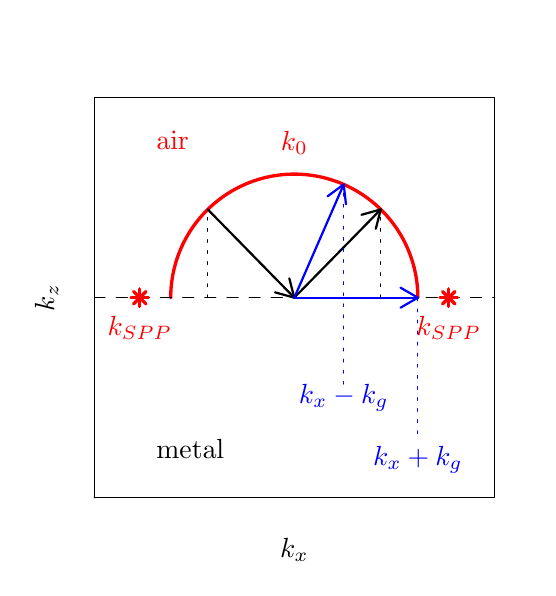
\begin{tikzpicture}[x=1pt,y=1pt]
\definecolor[named]{fillColor}{rgb}{1.00,1.00,1.00}
\path[use as bounding box,fill=fillColor,fill opacity=0.00] (0,0) rectangle (180.67,195.13);
\begin{scope}
\path[clip] (  0.00,  0.00) rectangle (180.67,195.13);
\definecolor[named]{drawColor}{rgb}{0.00,0.00,0.00}

\path[draw=drawColor,line width= 0.4pt,line join=round,line cap=round] ( 24.00, 25.23) --
	(168.67, 25.23) --
	(168.67,169.90) --
	( 24.00,169.90) --
	( 24.00, 25.23);

\node[text=drawColor,anchor=base,inner sep=0pt, outer sep=0pt, scale=  1.00] at ( 96.34,  3.63) {$k_x$};

\node[text=drawColor,rotate= 90.00,anchor=base,inner sep=0pt, outer sep=0pt, scale=  1.00] at (  9.60, 97.56) {$k_z$};
\end{scope}
\begin{scope}
\path[clip] ( 24.00, 25.23) rectangle (168.67,169.90);
\definecolor[named]{drawColor}{rgb}{1.00,0.00,0.00}

\path[draw=drawColor,line width= 1.2pt,line join=round,line cap=round] (140.99, 97.56) --
	(140.97, 98.98) --
	(140.90,100.40) --
	(140.79,101.81) --
	(140.63,103.22) --
	(140.43,104.62) --
	(140.18,106.02) --
	(139.89,107.40) --
	(139.56,108.78) --
	(139.18,110.14) --
	(138.76,111.50) --
	(138.30,112.84) --
	(137.79,114.16) --
	(137.24,115.47) --
	(136.66,116.76) --
	(136.03,118.03) --
	(135.36,119.27) --
	(134.65,120.50) --
	(133.90,121.71) --
	(133.12,122.89) --
	(132.30,124.04) --
	(131.44,125.17) --
	(130.54,126.27) --
	(129.62,127.34) --
	(128.65,128.38) --
	(127.66,129.39) --
	(126.63,130.37) --
	(125.58,131.31) --
	(124.49,132.22) --
	(123.38,133.10) --
	(122.24,133.94) --
	(121.07,134.74) --
	(119.88,135.51) --
	(118.66,136.23) --
	(117.43,136.92) --
	(116.17,137.57) --
	(114.89,138.18) --
	(113.59,138.75) --
	(112.27,139.28) --
	(110.94,139.76) --
	(109.60,140.20) --
	(108.24,140.60) --
	(106.86,140.96) --
	(105.48,141.27) --
	(104.09,141.54) --
	(102.69,141.76) --
	(101.29,141.94) --
	( 99.88,142.08) --
	( 98.46,142.17) --
	( 97.05,142.21) --
	( 95.63,142.21) --
	( 94.21,142.17) --
	( 92.80,142.08) --
	( 91.39,141.94) --
	( 89.98,141.76) --
	( 88.58,141.54) --
	( 87.19,141.27) --
	( 85.81,140.96) --
	( 84.44,140.60) --
	( 83.08,140.20) --
	( 81.73,139.76) --
	( 80.40,139.28) --
	( 79.09,138.75) --
	( 77.79,138.18) --
	( 76.51,137.57) --
	( 75.25,136.92) --
	( 74.01,136.23) --
	( 72.80,135.51) --
	( 71.60,134.74) --
	( 70.44,133.94) --
	( 69.30,133.10) --
	( 68.18,132.22) --
	( 67.10,131.31) --
	( 66.04,130.37) --
	( 65.01,129.39) --
	( 64.02,128.38) --
	( 63.06,127.34) --
	( 62.13,126.27) --
	( 61.24,125.17) --
	( 60.38,124.04) --
	( 59.56,122.89) --
	( 58.77,121.71) --
	( 58.03,120.50) --
	( 57.32,119.27) --
	( 56.65,118.03) --
	( 56.02,116.76) --
	( 55.43,115.47) --
	( 54.88,114.16) --
	( 54.38,112.84) --
	( 53.91,111.50) --
	( 53.49,110.14) --
	( 53.12,108.78) --
	( 52.78,107.40) --
	( 52.49,106.02) --
	( 52.25,104.62) --
	( 52.04,103.22) --
	( 51.89,101.81) --
	( 51.77,100.40) --
	( 51.71, 98.98) --
	( 51.68, 97.56);
\definecolor[named]{drawColor}{rgb}{0.00,0.00,0.00}

\path[draw=drawColor,line width= 0.4pt,dash pattern=on 4pt off 4pt ,line join=round,line cap=round] (  0.00, 97.56) --
	(  0.27, 97.56) --
	(  2.97, 97.56) --
	(  5.68, 97.56) --
	(  8.39, 97.56) --
	( 11.09, 97.56) --
	( 13.80, 97.56) --
	( 16.50, 97.56) --
	( 19.21, 97.56) --
	( 21.92, 97.56) --
	( 24.62, 97.56) --
	( 27.33, 97.56) --
	( 30.03, 97.56) --
	( 32.74, 97.56) --
	( 35.45, 97.56) --
	( 38.15, 97.56) --
	( 40.86, 97.56) --
	( 43.57, 97.56) --
	( 46.27, 97.56) --
	( 48.98, 97.56) --
	( 51.68, 97.56) --
	( 54.39, 97.56) --
	( 57.10, 97.56) --
	( 59.80, 97.56) --
	( 62.51, 97.56) --
	( 65.22, 97.56) --
	( 67.92, 97.56) --
	( 70.63, 97.56) --
	( 73.33, 97.56) --
	( 76.04, 97.56) --
	( 78.75, 97.56) --
	( 81.45, 97.56) --
	( 84.16, 97.56) --
	( 86.87, 97.56) --
	( 89.57, 97.56) --
	( 92.28, 97.56) --
	( 94.98, 97.56) --
	( 97.69, 97.56) --
	(100.40, 97.56) --
	(103.10, 97.56) --
	(105.81, 97.56) --
	(108.52, 97.56) --
	(111.22, 97.56) --
	(113.93, 97.56) --
	(116.63, 97.56) --
	(119.34, 97.56) --
	(122.05, 97.56) --
	(124.75, 97.56) --
	(127.46, 97.56) --
	(130.17, 97.56) --
	(132.87, 97.56) --
	(135.58, 97.56) --
	(138.28, 97.56) --
	(140.99, 97.56) --
	(143.70, 97.56) --
	(146.40, 97.56) --
	(149.11, 97.56) --
	(151.82, 97.56) --
	(154.52, 97.56) --
	(157.23, 97.56) --
	(159.93, 97.56) --
	(162.64, 97.56) --
	(165.35, 97.56) --
	(168.05, 97.56) --
	(170.76, 97.56) --
	(173.47, 97.56) --
	(176.17, 97.56) --
	(178.88, 97.56) --
	(180.67, 97.56);
\definecolor[named]{drawColor}{rgb}{1.00,0.00,0.00}

\path[draw=drawColor,line width= 1.2pt,line join=round,line cap=round] ( 38.27, 95.31) -- ( 42.77, 99.81);

\path[draw=drawColor,line width= 1.2pt,line join=round,line cap=round] ( 38.27, 99.81) -- ( 42.77, 95.31);

\path[draw=drawColor,line width= 1.2pt,line join=round,line cap=round] ( 37.34, 97.56) -- ( 43.70, 97.56);

\path[draw=drawColor,line width= 1.2pt,line join=round,line cap=round] ( 40.52, 94.38) -- ( 40.52,100.75);

\path[draw=drawColor,line width= 1.2pt,line join=round,line cap=round] (149.90, 95.31) -- (154.40, 99.81);

\path[draw=drawColor,line width= 1.2pt,line join=round,line cap=round] (149.90, 99.81) -- (154.40, 95.31);

\path[draw=drawColor,line width= 1.2pt,line join=round,line cap=round] (148.97, 97.56) -- (155.34, 97.56);

\path[draw=drawColor,line width= 1.2pt,line join=round,line cap=round] (152.15, 94.38) -- (152.15,100.75);
\definecolor[named]{drawColor}{rgb}{0.00,0.00,0.00}

\path[draw=drawColor,line width= 1.2pt,line join=round,line cap=round] ( 15.95, 95.31) -- ( 20.45, 99.81);

\path[draw=drawColor,line width= 1.2pt,line join=round,line cap=round] ( 15.95, 99.81) -- ( 20.45, 95.31);

\path[draw=drawColor,line width= 1.2pt,line join=round,line cap=round] ( 15.01, 97.56) -- ( 21.38, 97.56);

\path[draw=drawColor,line width= 1.2pt,line join=round,line cap=round] ( 18.20, 94.38) -- ( 18.20,100.75);

\path[draw=drawColor,line width= 1.2pt,line join=round,line cap=round] (172.23, 95.31) -- (176.73, 99.81);

\path[draw=drawColor,line width= 1.2pt,line join=round,line cap=round] (172.23, 99.81) -- (176.73, 95.31);

\path[draw=drawColor,line width= 1.2pt,line join=round,line cap=round] (171.30, 97.56) -- (177.66, 97.56);

\path[draw=drawColor,line width= 1.2pt,line join=round,line cap=round] (174.48, 94.38) -- (174.48,100.75);

\path[] ( 74.01,146.68) rectangle (118.66,157.85);
\definecolor[named]{drawColor}{rgb}{1.00,0.00,0.00}

\node[text=drawColor,anchor=base,inner sep=0pt, outer sep=0pt, scale=  1.00] at ( 96.34,150.80) {$k_0$};

\node[text=drawColor,anchor=base west,inner sep=0pt, outer sep=0pt, scale=  1.00] at ( 46.52,151.08) {air};
\definecolor[named]{drawColor}{rgb}{0.00,0.00,0.00}

\node[text=drawColor,anchor=base west,inner sep=0pt, outer sep=0pt, scale=  1.00] at ( 46.52, 39.45) {metal};
\definecolor[named]{drawColor}{rgb}{1.00,0.00,0.00}

\node[text=drawColor,anchor=base,inner sep=0pt, outer sep=0pt, scale=  1.00] at (152.15, 83.90) {$k_{SPP}$};

\node[text=drawColor,anchor=base,inner sep=0pt, outer sep=0pt, scale=  1.00] at ( 40.52, 83.90) {$k_{SPP}$};
\definecolor[named]{drawColor}{rgb}{0.00,0.00,0.00}

\path[draw=drawColor,line width= 0.8pt,line join=round,line cap=round] ( 65.08,129.45) -- ( 96.34, 97.56);

\path[draw=drawColor,line width= 0.8pt,line join=round,line cap=round] ( 89.38, 99.50) --
	( 96.34, 97.56) --
	( 94.54,104.56);

\path[draw=drawColor,line width= 0.8pt,line join=round,line cap=round] ( 96.34, 97.56) -- (127.59,129.45);

\path[draw=drawColor,line width= 0.8pt,line join=round,line cap=round] (125.79,122.45) --
	(127.59,129.45) --
	(120.63,127.51);
\definecolor[named]{drawColor}{rgb}{0.00,0.00,1.00}

\path[draw=drawColor,line width= 0.8pt,line join=round,line cap=round] ( 96.34, 97.56) -- (140.99, 97.56);

\path[draw=drawColor,line width= 0.8pt,line join=round,line cap=round] (134.73, 93.95) --
	(140.99, 97.56) --
	(134.73,101.18);

\path[draw=drawColor,line width= 0.8pt,line join=round,line cap=round] ( 96.34, 97.56) -- (114.20,138.49);

\path[draw=drawColor,line width= 0.8pt,line join=round,line cap=round] (115.01,131.31) --
	(114.20,138.49) --
	(108.38,134.20);
\definecolor[named]{drawColor}{rgb}{0.00,0.00,0.00}

\path[draw=drawColor,line width= 0.4pt,dash pattern=on 1pt off 3pt ,line join=round,line cap=round] ( 65.08, 97.56) --
	( 65.08, 97.89) --
	( 65.08, 98.21) --
	( 65.08, 98.53) --
	( 65.08, 98.85) --
	( 65.08, 99.18) --
	( 65.08, 99.50) --
	( 65.08, 99.82) --
	( 65.08,100.14) --
	( 65.08,100.46) --
	( 65.08,100.79) --
	( 65.08,101.11) --
	( 65.08,101.43) --
	( 65.08,101.75) --
	( 65.08,102.07) --
	( 65.08,102.40) --
	( 65.08,102.72) --
	( 65.08,103.04) --
	( 65.08,103.36) --
	( 65.08,103.68) --
	( 65.08,104.01) --
	( 65.08,104.33) --
	( 65.08,104.65) --
	( 65.08,104.97) --
	( 65.08,105.30) --
	( 65.08,105.62) --
	( 65.08,105.94) --
	( 65.08,106.26) --
	( 65.08,106.58) --
	( 65.08,106.91) --
	( 65.08,107.23) --
	( 65.08,107.55) --
	( 65.08,107.87) --
	( 65.08,108.19) --
	( 65.08,108.52) --
	( 65.08,108.84) --
	( 65.08,109.16) --
	( 65.08,109.48) --
	( 65.08,109.80) --
	( 65.08,110.13) --
	( 65.08,110.45) --
	( 65.08,110.77) --
	( 65.08,111.09) --
	( 65.08,111.42) --
	( 65.08,111.74) --
	( 65.08,112.06) --
	( 65.08,112.38) --
	( 65.08,112.70) --
	( 65.08,113.03) --
	( 65.08,113.35) --
	( 65.08,113.67) --
	( 65.08,113.99) --
	( 65.08,114.31) --
	( 65.08,114.64) --
	( 65.08,114.96) --
	( 65.08,115.28) --
	( 65.08,115.60) --
	( 65.08,115.92) --
	( 65.08,116.25) --
	( 65.08,116.57) --
	( 65.08,116.89) --
	( 65.08,117.21) --
	( 65.08,117.54) --
	( 65.08,117.86) --
	( 65.08,118.18) --
	( 65.08,118.50) --
	( 65.08,118.82) --
	( 65.08,119.15) --
	( 65.08,119.47) --
	( 65.08,119.79) --
	( 65.08,120.11) --
	( 65.08,120.43) --
	( 65.08,120.76) --
	( 65.08,121.08) --
	( 65.08,121.40) --
	( 65.08,121.72) --
	( 65.08,122.04) --
	( 65.08,122.37) --
	( 65.08,122.69) --
	( 65.08,123.01) --
	( 65.08,123.33) --
	( 65.08,123.66) --
	( 65.08,123.98) --
	( 65.08,124.30) --
	( 65.08,124.62) --
	( 65.08,124.94) --
	( 65.08,125.27) --
	( 65.08,125.59) --
	( 65.08,125.91) --
	( 65.08,126.23) --
	( 65.08,126.55) --
	( 65.08,126.88) --
	( 65.08,127.20) --
	( 65.08,127.52) --
	( 65.08,127.84) --
	( 65.08,128.16) --
	( 65.08,128.49) --
	( 65.08,128.81) --
	( 65.08,129.13) --
	( 65.08,129.45);

\path[draw=drawColor,line width= 0.4pt,dash pattern=on 1pt off 3pt ,line join=round,line cap=round] (127.59, 97.56) --
	(127.59, 97.89) --
	(127.59, 98.21) --
	(127.59, 98.53) --
	(127.59, 98.85) --
	(127.59, 99.18) --
	(127.59, 99.50) --
	(127.59, 99.82) --
	(127.59,100.14) --
	(127.59,100.46) --
	(127.59,100.79) --
	(127.59,101.11) --
	(127.59,101.43) --
	(127.59,101.75) --
	(127.59,102.07) --
	(127.59,102.40) --
	(127.59,102.72) --
	(127.59,103.04) --
	(127.59,103.36) --
	(127.59,103.68) --
	(127.59,104.01) --
	(127.59,104.33) --
	(127.59,104.65) --
	(127.59,104.97) --
	(127.59,105.30) --
	(127.59,105.62) --
	(127.59,105.94) --
	(127.59,106.26) --
	(127.59,106.58) --
	(127.59,106.91) --
	(127.59,107.23) --
	(127.59,107.55) --
	(127.59,107.87) --
	(127.59,108.19) --
	(127.59,108.52) --
	(127.59,108.84) --
	(127.59,109.16) --
	(127.59,109.48) --
	(127.59,109.80) --
	(127.59,110.13) --
	(127.59,110.45) --
	(127.59,110.77) --
	(127.59,111.09) --
	(127.59,111.42) --
	(127.59,111.74) --
	(127.59,112.06) --
	(127.59,112.38) --
	(127.59,112.70) --
	(127.59,113.03) --
	(127.59,113.35) --
	(127.59,113.67) --
	(127.59,113.99) --
	(127.59,114.31) --
	(127.59,114.64) --
	(127.59,114.96) --
	(127.59,115.28) --
	(127.59,115.60) --
	(127.59,115.92) --
	(127.59,116.25) --
	(127.59,116.57) --
	(127.59,116.89) --
	(127.59,117.21) --
	(127.59,117.54) --
	(127.59,117.86) --
	(127.59,118.18) --
	(127.59,118.50) --
	(127.59,118.82) --
	(127.59,119.15) --
	(127.59,119.47) --
	(127.59,119.79) --
	(127.59,120.11) --
	(127.59,120.43) --
	(127.59,120.76) --
	(127.59,121.08) --
	(127.59,121.40) --
	(127.59,121.72) --
	(127.59,122.04) --
	(127.59,122.37) --
	(127.59,122.69) --
	(127.59,123.01) --
	(127.59,123.33) --
	(127.59,123.66) --
	(127.59,123.98) --
	(127.59,124.30) --
	(127.59,124.62) --
	(127.59,124.94) --
	(127.59,125.27) --
	(127.59,125.59) --
	(127.59,125.91) --
	(127.59,126.23) --
	(127.59,126.55) --
	(127.59,126.88) --
	(127.59,127.20) --
	(127.59,127.52) --
	(127.59,127.84) --
	(127.59,128.16) --
	(127.59,128.49) --
	(127.59,128.81) --
	(127.59,129.13) --
	(127.59,129.45);
\definecolor[named]{drawColor}{rgb}{0.00,0.00,1.00}

\path[draw=drawColor,line width= 0.4pt,dash pattern=on 1pt off 3pt ,line join=round,line cap=round] (140.99, 48.45) --
	(140.99, 48.94) --
	(140.99, 49.44) --
	(140.99, 49.93) --
	(140.99, 50.43) --
	(140.99, 50.93) --
	(140.99, 51.42) --
	(140.99, 51.92) --
	(140.99, 52.42) --
	(140.99, 52.91) --
	(140.99, 53.41) --
	(140.99, 53.90) --
	(140.99, 54.40) --
	(140.99, 54.90) --
	(140.99, 55.39) --
	(140.99, 55.89) --
	(140.99, 56.38) --
	(140.99, 56.88) --
	(140.99, 57.38) --
	(140.99, 57.87) --
	(140.99, 58.37) --
	(140.99, 58.87) --
	(140.99, 59.36) --
	(140.99, 59.86) --
	(140.99, 60.35) --
	(140.99, 60.85) --
	(140.99, 61.35) --
	(140.99, 61.84) --
	(140.99, 62.34) --
	(140.99, 62.83) --
	(140.99, 63.33) --
	(140.99, 63.83) --
	(140.99, 64.32) --
	(140.99, 64.82) --
	(140.99, 65.32) --
	(140.99, 65.81) --
	(140.99, 66.31) --
	(140.99, 66.80) --
	(140.99, 67.30) --
	(140.99, 67.80) --
	(140.99, 68.29) --
	(140.99, 68.79) --
	(140.99, 69.28) --
	(140.99, 69.78) --
	(140.99, 70.28) --
	(140.99, 70.77) --
	(140.99, 71.27) --
	(140.99, 71.77) --
	(140.99, 72.26) --
	(140.99, 72.76) --
	(140.99, 73.25) --
	(140.99, 73.75) --
	(140.99, 74.25) --
	(140.99, 74.74) --
	(140.99, 75.24) --
	(140.99, 75.73) --
	(140.99, 76.23) --
	(140.99, 76.73) --
	(140.99, 77.22) --
	(140.99, 77.72) --
	(140.99, 78.21) --
	(140.99, 78.71) --
	(140.99, 79.21) --
	(140.99, 79.70) --
	(140.99, 80.20) --
	(140.99, 80.70) --
	(140.99, 81.19) --
	(140.99, 81.69) --
	(140.99, 82.18) --
	(140.99, 82.68) --
	(140.99, 83.18) --
	(140.99, 83.67) --
	(140.99, 84.17) --
	(140.99, 84.66) --
	(140.99, 85.16) --
	(140.99, 85.66) --
	(140.99, 86.15) --
	(140.99, 86.65) --
	(140.99, 87.15) --
	(140.99, 87.64) --
	(140.99, 88.14) --
	(140.99, 88.63) --
	(140.99, 89.13) --
	(140.99, 89.63) --
	(140.99, 90.12) --
	(140.99, 90.62) --
	(140.99, 91.11) --
	(140.99, 91.61) --
	(140.99, 92.11) --
	(140.99, 92.60) --
	(140.99, 93.10) --
	(140.99, 93.60) --
	(140.99, 94.09) --
	(140.99, 94.59) --
	(140.99, 95.08) --
	(140.99, 95.58) --
	(140.99, 96.08) --
	(140.99, 96.57) --
	(140.99, 97.07) --
	(140.99, 97.56);

\path[draw=drawColor,line width= 0.4pt,dash pattern=on 1pt off 3pt ,line join=round,line cap=round] (114.20, 66.31) --
	(114.20, 67.04) --
	(114.20, 67.77) --
	(114.20, 68.49) --
	(114.20, 69.22) --
	(114.20, 69.95) --
	(114.20, 70.68) --
	(114.20, 71.41) --
	(114.20, 72.14) --
	(114.20, 72.87) --
	(114.20, 73.60) --
	(114.20, 74.33) --
	(114.20, 75.06) --
	(114.20, 75.79) --
	(114.20, 76.52) --
	(114.20, 77.24) --
	(114.20, 77.97) --
	(114.20, 78.70) --
	(114.20, 79.43) --
	(114.20, 80.16) --
	(114.20, 80.89) --
	(114.20, 81.62) --
	(114.20, 82.35) --
	(114.20, 83.08) --
	(114.20, 83.81) --
	(114.20, 84.54) --
	(114.20, 85.26) --
	(114.20, 85.99) --
	(114.20, 86.72) --
	(114.20, 87.45) --
	(114.20, 88.18) --
	(114.20, 88.91) --
	(114.20, 89.64) --
	(114.20, 90.37) --
	(114.20, 91.10) --
	(114.20, 91.83) --
	(114.20, 92.56) --
	(114.20, 93.28) --
	(114.20, 94.01) --
	(114.20, 94.74) --
	(114.20, 95.47) --
	(114.20, 96.20) --
	(114.20, 96.93) --
	(114.20, 97.66) --
	(114.20, 98.39) --
	(114.20, 99.12) --
	(114.20, 99.85) --
	(114.20,100.58) --
	(114.20,101.30) --
	(114.20,102.03) --
	(114.20,102.76) --
	(114.20,103.49) --
	(114.20,104.22) --
	(114.20,104.95) --
	(114.20,105.68) --
	(114.20,106.41) --
	(114.20,107.14) --
	(114.20,107.87) --
	(114.20,108.60) --
	(114.20,109.33) --
	(114.20,110.05) --
	(114.20,110.78) --
	(114.20,111.51) --
	(114.20,112.24) --
	(114.20,112.97) --
	(114.20,113.70) --
	(114.20,114.43) --
	(114.20,115.16) --
	(114.20,115.89) --
	(114.20,116.62) --
	(114.20,117.35) --
	(114.20,118.07) --
	(114.20,118.80) --
	(114.20,119.53) --
	(114.20,120.26) --
	(114.20,120.99) --
	(114.20,121.72) --
	(114.20,122.45) --
	(114.20,123.18) --
	(114.20,123.91) --
	(114.20,124.64) --
	(114.20,125.37) --
	(114.20,126.09) --
	(114.20,126.82) --
	(114.20,127.55) --
	(114.20,128.28) --
	(114.20,129.01) --
	(114.20,129.74) --
	(114.20,130.47) --
	(114.20,131.20) --
	(114.20,131.93) --
	(114.20,132.66) --
	(114.20,133.39) --
	(114.20,134.11) --
	(114.20,134.84) --
	(114.20,135.57) --
	(114.20,136.30) --
	(114.20,137.03) --
	(114.20,137.76) --
	(114.20,138.49);

\node[text=drawColor,anchor=base,inner sep=0pt, outer sep=0pt, scale=  1.00] at (140.99, 36.93) {$k_x+k_g$};

\node[text=drawColor,anchor=base,inner sep=0pt, outer sep=0pt, scale=  1.00] at (114.20, 59.26) {$k_x-k_g$};
\end{scope}
\end{tikzpicture}
\label{fig:grating-indexiticesB}}
\subfigure[]{% Created by tikzDevice version 0.6.2-92-0ad2792 on 2012-09-24 19:13:06
% !TEX encoding = UTF-8 Unicode
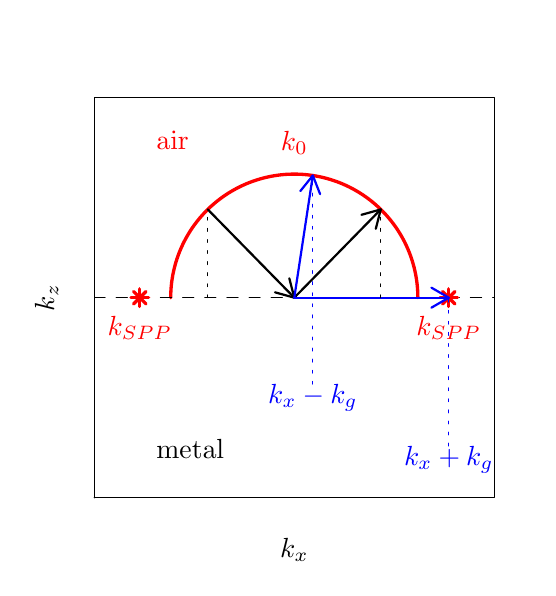
\begin{tikzpicture}[x=1pt,y=1pt]
\definecolor[named]{fillColor}{rgb}{1.00,1.00,1.00}
\path[use as bounding box,fill=fillColor,fill opacity=0.00] (0,0) rectangle (180.67,195.13);
\begin{scope}
\path[clip] (  0.00,  0.00) rectangle (180.67,195.13);
\definecolor[named]{drawColor}{rgb}{0.00,0.00,0.00}

\path[draw=drawColor,line width= 0.4pt,line join=round,line cap=round] ( 24.00, 25.23) --
	(168.67, 25.23) --
	(168.67,169.90) --
	( 24.00,169.90) --
	( 24.00, 25.23);

\node[text=drawColor,anchor=base,inner sep=0pt, outer sep=0pt, scale=  1.00] at ( 96.34,  3.63) {$k_x$};

\node[text=drawColor,rotate= 90.00,anchor=base,inner sep=0pt, outer sep=0pt, scale=  1.00] at (  9.60, 97.56) {$k_z$};
\end{scope}
\begin{scope}
\path[clip] ( 24.00, 25.23) rectangle (168.67,169.90);
\definecolor[named]{drawColor}{rgb}{1.00,0.00,0.00}

\path[draw=drawColor,line width= 1.2pt,line join=round,line cap=round] (140.99, 97.56) --
	(140.97, 98.98) --
	(140.90,100.40) --
	(140.79,101.81) --
	(140.63,103.22) --
	(140.43,104.62) --
	(140.18,106.02) --
	(139.89,107.40) --
	(139.56,108.78) --
	(139.18,110.14) --
	(138.76,111.50) --
	(138.30,112.84) --
	(137.79,114.16) --
	(137.24,115.47) --
	(136.66,116.76) --
	(136.03,118.03) --
	(135.36,119.27) --
	(134.65,120.50) --
	(133.90,121.71) --
	(133.12,122.89) --
	(132.30,124.04) --
	(131.44,125.17) --
	(130.54,126.27) --
	(129.62,127.34) --
	(128.65,128.38) --
	(127.66,129.39) --
	(126.63,130.37) --
	(125.58,131.31) --
	(124.49,132.22) --
	(123.38,133.10) --
	(122.24,133.94) --
	(121.07,134.74) --
	(119.88,135.51) --
	(118.66,136.23) --
	(117.43,136.92) --
	(116.17,137.57) --
	(114.89,138.18) --
	(113.59,138.75) --
	(112.27,139.28) --
	(110.94,139.76) --
	(109.60,140.20) --
	(108.24,140.60) --
	(106.86,140.96) --
	(105.48,141.27) --
	(104.09,141.54) --
	(102.69,141.76) --
	(101.29,141.94) --
	( 99.88,142.08) --
	( 98.46,142.17) --
	( 97.05,142.21) --
	( 95.63,142.21) --
	( 94.21,142.17) --
	( 92.80,142.08) --
	( 91.39,141.94) --
	( 89.98,141.76) --
	( 88.58,141.54) --
	( 87.19,141.27) --
	( 85.81,140.96) --
	( 84.44,140.60) --
	( 83.08,140.20) --
	( 81.73,139.76) --
	( 80.40,139.28) --
	( 79.09,138.75) --
	( 77.79,138.18) --
	( 76.51,137.57) --
	( 75.25,136.92) --
	( 74.01,136.23) --
	( 72.80,135.51) --
	( 71.60,134.74) --
	( 70.44,133.94) --
	( 69.30,133.10) --
	( 68.18,132.22) --
	( 67.10,131.31) --
	( 66.04,130.37) --
	( 65.01,129.39) --
	( 64.02,128.38) --
	( 63.06,127.34) --
	( 62.13,126.27) --
	( 61.24,125.17) --
	( 60.38,124.04) --
	( 59.56,122.89) --
	( 58.77,121.71) --
	( 58.03,120.50) --
	( 57.32,119.27) --
	( 56.65,118.03) --
	( 56.02,116.76) --
	( 55.43,115.47) --
	( 54.88,114.16) --
	( 54.38,112.84) --
	( 53.91,111.50) --
	( 53.49,110.14) --
	( 53.12,108.78) --
	( 52.78,107.40) --
	( 52.49,106.02) --
	( 52.25,104.62) --
	( 52.04,103.22) --
	( 51.89,101.81) --
	( 51.77,100.40) --
	( 51.71, 98.98) --
	( 51.68, 97.56);
\definecolor[named]{drawColor}{rgb}{0.00,0.00,0.00}

\path[draw=drawColor,line width= 0.4pt,dash pattern=on 4pt off 4pt ,line join=round,line cap=round] (  0.00, 97.56) --
	(  0.27, 97.56) --
	(  2.97, 97.56) --
	(  5.68, 97.56) --
	(  8.39, 97.56) --
	( 11.09, 97.56) --
	( 13.80, 97.56) --
	( 16.50, 97.56) --
	( 19.21, 97.56) --
	( 21.92, 97.56) --
	( 24.62, 97.56) --
	( 27.33, 97.56) --
	( 30.03, 97.56) --
	( 32.74, 97.56) --
	( 35.45, 97.56) --
	( 38.15, 97.56) --
	( 40.86, 97.56) --
	( 43.57, 97.56) --
	( 46.27, 97.56) --
	( 48.98, 97.56) --
	( 51.68, 97.56) --
	( 54.39, 97.56) --
	( 57.10, 97.56) --
	( 59.80, 97.56) --
	( 62.51, 97.56) --
	( 65.22, 97.56) --
	( 67.92, 97.56) --
	( 70.63, 97.56) --
	( 73.33, 97.56) --
	( 76.04, 97.56) --
	( 78.75, 97.56) --
	( 81.45, 97.56) --
	( 84.16, 97.56) --
	( 86.87, 97.56) --
	( 89.57, 97.56) --
	( 92.28, 97.56) --
	( 94.98, 97.56) --
	( 97.69, 97.56) --
	(100.40, 97.56) --
	(103.10, 97.56) --
	(105.81, 97.56) --
	(108.52, 97.56) --
	(111.22, 97.56) --
	(113.93, 97.56) --
	(116.63, 97.56) --
	(119.34, 97.56) --
	(122.05, 97.56) --
	(124.75, 97.56) --
	(127.46, 97.56) --
	(130.17, 97.56) --
	(132.87, 97.56) --
	(135.58, 97.56) --
	(138.28, 97.56) --
	(140.99, 97.56) --
	(143.70, 97.56) --
	(146.40, 97.56) --
	(149.11, 97.56) --
	(151.82, 97.56) --
	(154.52, 97.56) --
	(157.23, 97.56) --
	(159.93, 97.56) --
	(162.64, 97.56) --
	(165.35, 97.56) --
	(168.05, 97.56) --
	(170.76, 97.56) --
	(173.47, 97.56) --
	(176.17, 97.56) --
	(178.88, 97.56) --
	(180.67, 97.56);
\definecolor[named]{drawColor}{rgb}{1.00,0.00,0.00}

\path[draw=drawColor,line width= 1.2pt,line join=round,line cap=round] ( 38.27, 95.31) -- ( 42.77, 99.81);

\path[draw=drawColor,line width= 1.2pt,line join=round,line cap=round] ( 38.27, 99.81) -- ( 42.77, 95.31);

\path[draw=drawColor,line width= 1.2pt,line join=round,line cap=round] ( 37.34, 97.56) -- ( 43.70, 97.56);

\path[draw=drawColor,line width= 1.2pt,line join=round,line cap=round] ( 40.52, 94.38) -- ( 40.52,100.75);

\path[draw=drawColor,line width= 1.2pt,line join=round,line cap=round] (149.90, 95.31) -- (154.40, 99.81);

\path[draw=drawColor,line width= 1.2pt,line join=round,line cap=round] (149.90, 99.81) -- (154.40, 95.31);

\path[draw=drawColor,line width= 1.2pt,line join=round,line cap=round] (148.97, 97.56) -- (155.34, 97.56);

\path[draw=drawColor,line width= 1.2pt,line join=round,line cap=round] (152.15, 94.38) -- (152.15,100.75);
\definecolor[named]{drawColor}{rgb}{0.00,0.00,0.00}

\path[draw=drawColor,line width= 1.2pt,line join=round,line cap=round] ( 15.95, 95.31) -- ( 20.45, 99.81);

\path[draw=drawColor,line width= 1.2pt,line join=round,line cap=round] ( 15.95, 99.81) -- ( 20.45, 95.31);

\path[draw=drawColor,line width= 1.2pt,line join=round,line cap=round] ( 15.01, 97.56) -- ( 21.38, 97.56);

\path[draw=drawColor,line width= 1.2pt,line join=round,line cap=round] ( 18.20, 94.38) -- ( 18.20,100.75);

\path[draw=drawColor,line width= 1.2pt,line join=round,line cap=round] (172.23, 95.31) -- (176.73, 99.81);

\path[draw=drawColor,line width= 1.2pt,line join=round,line cap=round] (172.23, 99.81) -- (176.73, 95.31);

\path[draw=drawColor,line width= 1.2pt,line join=round,line cap=round] (171.30, 97.56) -- (177.66, 97.56);

\path[draw=drawColor,line width= 1.2pt,line join=round,line cap=round] (174.48, 94.38) -- (174.48,100.75);

\path[] ( 74.01,146.68) rectangle (118.66,157.85);
\definecolor[named]{drawColor}{rgb}{1.00,0.00,0.00}

\node[text=drawColor,anchor=base,inner sep=0pt, outer sep=0pt, scale=  1.00] at ( 96.34,150.80) {$k_0$};

\node[text=drawColor,anchor=base west,inner sep=0pt, outer sep=0pt, scale=  1.00] at ( 46.52,151.08) {air};
\definecolor[named]{drawColor}{rgb}{0.00,0.00,0.00}

\node[text=drawColor,anchor=base west,inner sep=0pt, outer sep=0pt, scale=  1.00] at ( 46.52, 39.45) {metal};
\definecolor[named]{drawColor}{rgb}{1.00,0.00,0.00}

\node[text=drawColor,anchor=base,inner sep=0pt, outer sep=0pt, scale=  1.00] at (152.15, 83.90) {$k_{SPP}$};

\node[text=drawColor,anchor=base,inner sep=0pt, outer sep=0pt, scale=  1.00] at ( 40.52, 83.90) {$k_{SPP}$};
\definecolor[named]{drawColor}{rgb}{0.00,0.00,0.00}

\path[draw=drawColor,line width= 0.8pt,line join=round,line cap=round] ( 65.08,129.45) -- ( 96.34, 97.56);

\path[draw=drawColor,line width= 0.8pt,line join=round,line cap=round] ( 89.38, 99.50) --
	( 96.34, 97.56) --
	( 94.54,104.56);

\path[draw=drawColor,line width= 0.8pt,line join=round,line cap=round] ( 96.34, 97.56) -- (127.59,129.45);

\path[draw=drawColor,line width= 0.8pt,line join=round,line cap=round] (125.79,122.45) --
	(127.59,129.45) --
	(120.63,127.51);
\definecolor[named]{drawColor}{rgb}{0.00,0.00,1.00}

\path[draw=drawColor,line width= 0.8pt,line join=round,line cap=round] ( 96.34, 97.56) -- (152.15, 97.56);

\path[draw=drawColor,line width= 0.8pt,line join=round,line cap=round] (145.89, 93.95) --
	(152.15, 97.56) --
	(145.89,101.18);

\path[draw=drawColor,line width= 0.8pt,line join=round,line cap=round] ( 96.34, 97.56) -- (103.04,141.71);

\path[draw=drawColor,line width= 0.8pt,line join=round,line cap=round] (105.67,134.98) --
	(103.04,141.71) --
	( 98.52,136.07);

\path[] ( 91.87, 75.24) rectangle (114.20, 84.17);
\definecolor[named]{drawColor}{rgb}{0.00,0.00,0.00}

\path[draw=drawColor,line width= 0.4pt,dash pattern=on 1pt off 3pt ,line join=round,line cap=round] ( 65.08, 97.56) --
	( 65.08, 97.89) --
	( 65.08, 98.21) --
	( 65.08, 98.53) --
	( 65.08, 98.85) --
	( 65.08, 99.18) --
	( 65.08, 99.50) --
	( 65.08, 99.82) --
	( 65.08,100.14) --
	( 65.08,100.46) --
	( 65.08,100.79) --
	( 65.08,101.11) --
	( 65.08,101.43) --
	( 65.08,101.75) --
	( 65.08,102.07) --
	( 65.08,102.40) --
	( 65.08,102.72) --
	( 65.08,103.04) --
	( 65.08,103.36) --
	( 65.08,103.68) --
	( 65.08,104.01) --
	( 65.08,104.33) --
	( 65.08,104.65) --
	( 65.08,104.97) --
	( 65.08,105.30) --
	( 65.08,105.62) --
	( 65.08,105.94) --
	( 65.08,106.26) --
	( 65.08,106.58) --
	( 65.08,106.91) --
	( 65.08,107.23) --
	( 65.08,107.55) --
	( 65.08,107.87) --
	( 65.08,108.19) --
	( 65.08,108.52) --
	( 65.08,108.84) --
	( 65.08,109.16) --
	( 65.08,109.48) --
	( 65.08,109.80) --
	( 65.08,110.13) --
	( 65.08,110.45) --
	( 65.08,110.77) --
	( 65.08,111.09) --
	( 65.08,111.42) --
	( 65.08,111.74) --
	( 65.08,112.06) --
	( 65.08,112.38) --
	( 65.08,112.70) --
	( 65.08,113.03) --
	( 65.08,113.35) --
	( 65.08,113.67) --
	( 65.08,113.99) --
	( 65.08,114.31) --
	( 65.08,114.64) --
	( 65.08,114.96) --
	( 65.08,115.28) --
	( 65.08,115.60) --
	( 65.08,115.92) --
	( 65.08,116.25) --
	( 65.08,116.57) --
	( 65.08,116.89) --
	( 65.08,117.21) --
	( 65.08,117.54) --
	( 65.08,117.86) --
	( 65.08,118.18) --
	( 65.08,118.50) --
	( 65.08,118.82) --
	( 65.08,119.15) --
	( 65.08,119.47) --
	( 65.08,119.79) --
	( 65.08,120.11) --
	( 65.08,120.43) --
	( 65.08,120.76) --
	( 65.08,121.08) --
	( 65.08,121.40) --
	( 65.08,121.72) --
	( 65.08,122.04) --
	( 65.08,122.37) --
	( 65.08,122.69) --
	( 65.08,123.01) --
	( 65.08,123.33) --
	( 65.08,123.66) --
	( 65.08,123.98) --
	( 65.08,124.30) --
	( 65.08,124.62) --
	( 65.08,124.94) --
	( 65.08,125.27) --
	( 65.08,125.59) --
	( 65.08,125.91) --
	( 65.08,126.23) --
	( 65.08,126.55) --
	( 65.08,126.88) --
	( 65.08,127.20) --
	( 65.08,127.52) --
	( 65.08,127.84) --
	( 65.08,128.16) --
	( 65.08,128.49) --
	( 65.08,128.81) --
	( 65.08,129.13) --
	( 65.08,129.45);

\path[draw=drawColor,line width= 0.4pt,dash pattern=on 1pt off 3pt ,line join=round,line cap=round] (127.59, 97.56) --
	(127.59, 97.89) --
	(127.59, 98.21) --
	(127.59, 98.53) --
	(127.59, 98.85) --
	(127.59, 99.18) --
	(127.59, 99.50) --
	(127.59, 99.82) --
	(127.59,100.14) --
	(127.59,100.46) --
	(127.59,100.79) --
	(127.59,101.11) --
	(127.59,101.43) --
	(127.59,101.75) --
	(127.59,102.07) --
	(127.59,102.40) --
	(127.59,102.72) --
	(127.59,103.04) --
	(127.59,103.36) --
	(127.59,103.68) --
	(127.59,104.01) --
	(127.59,104.33) --
	(127.59,104.65) --
	(127.59,104.97) --
	(127.59,105.30) --
	(127.59,105.62) --
	(127.59,105.94) --
	(127.59,106.26) --
	(127.59,106.58) --
	(127.59,106.91) --
	(127.59,107.23) --
	(127.59,107.55) --
	(127.59,107.87) --
	(127.59,108.19) --
	(127.59,108.52) --
	(127.59,108.84) --
	(127.59,109.16) --
	(127.59,109.48) --
	(127.59,109.80) --
	(127.59,110.13) --
	(127.59,110.45) --
	(127.59,110.77) --
	(127.59,111.09) --
	(127.59,111.42) --
	(127.59,111.74) --
	(127.59,112.06) --
	(127.59,112.38) --
	(127.59,112.70) --
	(127.59,113.03) --
	(127.59,113.35) --
	(127.59,113.67) --
	(127.59,113.99) --
	(127.59,114.31) --
	(127.59,114.64) --
	(127.59,114.96) --
	(127.59,115.28) --
	(127.59,115.60) --
	(127.59,115.92) --
	(127.59,116.25) --
	(127.59,116.57) --
	(127.59,116.89) --
	(127.59,117.21) --
	(127.59,117.54) --
	(127.59,117.86) --
	(127.59,118.18) --
	(127.59,118.50) --
	(127.59,118.82) --
	(127.59,119.15) --
	(127.59,119.47) --
	(127.59,119.79) --
	(127.59,120.11) --
	(127.59,120.43) --
	(127.59,120.76) --
	(127.59,121.08) --
	(127.59,121.40) --
	(127.59,121.72) --
	(127.59,122.04) --
	(127.59,122.37) --
	(127.59,122.69) --
	(127.59,123.01) --
	(127.59,123.33) --
	(127.59,123.66) --
	(127.59,123.98) --
	(127.59,124.30) --
	(127.59,124.62) --
	(127.59,124.94) --
	(127.59,125.27) --
	(127.59,125.59) --
	(127.59,125.91) --
	(127.59,126.23) --
	(127.59,126.55) --
	(127.59,126.88) --
	(127.59,127.20) --
	(127.59,127.52) --
	(127.59,127.84) --
	(127.59,128.16) --
	(127.59,128.49) --
	(127.59,128.81) --
	(127.59,129.13) --
	(127.59,129.45);
\definecolor[named]{drawColor}{rgb}{0.00,0.00,1.00}

\path[draw=drawColor,line width= 0.4pt,dash pattern=on 1pt off 3pt ,line join=round,line cap=round] (103.04, 66.31) --
	(103.04, 67.07) --
	(103.04, 67.83) --
	(103.04, 68.59) --
	(103.04, 69.35) --
	(103.04, 70.12) --
	(103.04, 70.88) --
	(103.04, 71.64) --
	(103.04, 72.40) --
	(103.04, 73.16) --
	(103.04, 73.92) --
	(103.04, 74.69) --
	(103.04, 75.45) --
	(103.04, 76.21) --
	(103.04, 76.97) --
	(103.04, 77.73) --
	(103.04, 78.49) --
	(103.04, 79.26) --
	(103.04, 80.02) --
	(103.04, 80.78) --
	(103.04, 81.54) --
	(103.04, 82.30) --
	(103.04, 83.06) --
	(103.04, 83.83) --
	(103.04, 84.59) --
	(103.04, 85.35) --
	(103.04, 86.11) --
	(103.04, 86.87) --
	(103.04, 87.63) --
	(103.04, 88.40) --
	(103.04, 89.16) --
	(103.04, 89.92) --
	(103.04, 90.68) --
	(103.04, 91.44) --
	(103.04, 92.20) --
	(103.04, 92.97) --
	(103.04, 93.73) --
	(103.04, 94.49) --
	(103.04, 95.25) --
	(103.04, 96.01) --
	(103.04, 96.77) --
	(103.04, 97.54) --
	(103.04, 98.30) --
	(103.04, 99.06) --
	(103.04, 99.82) --
	(103.04,100.58) --
	(103.04,101.34) --
	(103.04,102.11) --
	(103.04,102.87) --
	(103.04,103.63) --
	(103.04,104.39) --
	(103.04,105.15) --
	(103.04,105.91) --
	(103.04,106.68) --
	(103.04,107.44) --
	(103.04,108.20) --
	(103.04,108.96) --
	(103.04,109.72) --
	(103.04,110.48) --
	(103.04,111.25) --
	(103.04,112.01) --
	(103.04,112.77) --
	(103.04,113.53) --
	(103.04,114.29) --
	(103.04,115.05) --
	(103.04,115.82) --
	(103.04,116.58) --
	(103.04,117.34) --
	(103.04,118.10) --
	(103.04,118.86) --
	(103.04,119.62) --
	(103.04,120.39) --
	(103.04,121.15) --
	(103.04,121.91) --
	(103.04,122.67) --
	(103.04,123.43) --
	(103.04,124.19) --
	(103.04,124.96) --
	(103.04,125.72) --
	(103.04,126.48) --
	(103.04,127.24) --
	(103.04,128.00) --
	(103.04,128.76) --
	(103.04,129.53) --
	(103.04,130.29) --
	(103.04,131.05) --
	(103.04,131.81) --
	(103.04,132.57) --
	(103.04,133.33) --
	(103.04,134.10) --
	(103.04,134.86) --
	(103.04,135.62) --
	(103.04,136.38) --
	(103.04,137.14) --
	(103.04,137.90) --
	(103.04,138.67) --
	(103.04,139.43) --
	(103.04,140.19) --
	(103.04,140.95) --
	(103.04,141.71);

\path[draw=drawColor,line width= 0.4pt,dash pattern=on 1pt off 3pt ,line join=round,line cap=round] (152.15, 43.98) --
	(152.15, 44.52) --
	(152.15, 45.06) --
	(152.15, 45.60) --
	(152.15, 46.15) --
	(152.15, 46.69) --
	(152.15, 47.23) --
	(152.15, 47.77) --
	(152.15, 48.31) --
	(152.15, 48.85) --
	(152.15, 49.39) --
	(152.15, 49.93) --
	(152.15, 50.48) --
	(152.15, 51.02) --
	(152.15, 51.56) --
	(152.15, 52.10) --
	(152.15, 52.64) --
	(152.15, 53.18) --
	(152.15, 53.72) --
	(152.15, 54.26) --
	(152.15, 54.81) --
	(152.15, 55.35) --
	(152.15, 55.89) --
	(152.15, 56.43) --
	(152.15, 56.97) --
	(152.15, 57.51) --
	(152.15, 58.05) --
	(152.15, 58.59) --
	(152.15, 59.14) --
	(152.15, 59.68) --
	(152.15, 60.22) --
	(152.15, 60.76) --
	(152.15, 61.30) --
	(152.15, 61.84) --
	(152.15, 62.38) --
	(152.15, 62.92) --
	(152.15, 63.47) --
	(152.15, 64.01) --
	(152.15, 64.55) --
	(152.15, 65.09) --
	(152.15, 65.63) --
	(152.15, 66.17) --
	(152.15, 66.71) --
	(152.15, 67.25) --
	(152.15, 67.80) --
	(152.15, 68.34) --
	(152.15, 68.88) --
	(152.15, 69.42) --
	(152.15, 69.96) --
	(152.15, 70.50) --
	(152.15, 71.04) --
	(152.15, 71.58) --
	(152.15, 72.13) --
	(152.15, 72.67) --
	(152.15, 73.21) --
	(152.15, 73.75) --
	(152.15, 74.29) --
	(152.15, 74.83) --
	(152.15, 75.37) --
	(152.15, 75.91) --
	(152.15, 76.46) --
	(152.15, 77.00) --
	(152.15, 77.54) --
	(152.15, 78.08) --
	(152.15, 78.62) --
	(152.15, 79.16) --
	(152.15, 79.70) --
	(152.15, 80.24) --
	(152.15, 80.79) --
	(152.15, 81.33) --
	(152.15, 81.87) --
	(152.15, 82.41) --
	(152.15, 82.95) --
	(152.15, 83.49) --
	(152.15, 84.03) --
	(152.15, 84.57) --
	(152.15, 85.12) --
	(152.15, 85.66) --
	(152.15, 86.20) --
	(152.15, 86.74) --
	(152.15, 87.28) --
	(152.15, 87.82) --
	(152.15, 88.36) --
	(152.15, 88.90) --
	(152.15, 89.45) --
	(152.15, 89.99) --
	(152.15, 90.53) --
	(152.15, 91.07) --
	(152.15, 91.61) --
	(152.15, 92.15) --
	(152.15, 92.69) --
	(152.15, 93.23) --
	(152.15, 93.78) --
	(152.15, 94.32) --
	(152.15, 94.86) --
	(152.15, 95.40) --
	(152.15, 95.94) --
	(152.15, 96.48) --
	(152.15, 97.02) --
	(152.15, 97.56);

\node[text=drawColor,anchor=base,inner sep=0pt, outer sep=0pt, scale=  1.00] at (152.15, 36.93) {$k_x+k_g$};

\node[text=drawColor,anchor=base,inner sep=0pt, outer sep=0pt, scale=  1.00] at (103.04, 59.26) {$k_x-k_g$};
\end{scope}
\end{tikzpicture}
\label{fig:grating-indexiticesC}}
\caption[The allowed real momentum states for light incident on three diffraction gratings.]{The allowed real momentum states for light incident on three diffraction gratings. The gratings reduce in period (increase in $k_g$) from (a) to (c). Points along the red circle are the possible momentum states for light in air ($k_0$). There is no corressponding circle in the metal halfspace as light in this medium is considered to be evanescently damped and so has no real value of momentum. The red stars show the momentum states for SPPs. \label{fig:grating-indexitices}}
\end{center}
\end{figure}

The three illustrations in figure \ref{fig:grating-indexitices} show the momentum-space diagrams for monochromatic light of frequency $\omega_0 (=ck_0)$ incident on three gratings of different pitch, at a fixed polar angle in the classical mount of $\phi=0^\circ$\footnote{For the conical mount, these allowed momentum states would form instead a hemisphere in three-dimensional $k$-space.}. 
The allowed real momentum states of propagating light are represented as a red circle of radius $k_0$. Conservation of energy requires that any vectors representing propagating light have a magnitude of $k_0$, and as such are represented as radial arrows of this circle. Points that lie outside of the red light circle possess greater momentum than the incident light circle and represent non-propagating (evanescent) light with imaginary momenta. The red stars on the diagram are the allowed momentum states of a surface plasmon polariton. The surface plasmon polariton momentum state lies at a finite real value of $k_x$, with no real value of $k_z$, indicating the surface mode has a purely imaginary value of $k_z$ and so evanesently decays normal to the surface while propagating along it. Notice the surface plasmon polariton state lies outside the light circle, illustrating that even grazing light possesses insufficient momentum to match that of the surface mode.

The in-plane ($k_x$) component of light momentum on a grating surface is altered by the addition of an integer number of grating vectors (equation \ref{eq:addgratinvector}).  In figure \ref{fig:grating-indexiticesA}, three possible scattering events of incident light are shown, a $+1k_g$, a $–1k_g$ and no scattering ($0k_g$).  The allowed momentum states of light with these new values of $k_x$ show that diffracted light must leave the surface at a different polar angle to the specular reflection ($0k_g$) to conserve total momentum, $k_0$ (and so still lie on the radial line of constant total momentum). This angle of diffraction is dependent on the size of the light circle, determined by the frequency of the radiation, which illustrates the dispersive properties of a diffraction grating.
The grating represented in figure \ref{fig:grating-indexiticesB} has a periodicity less than that of grating \ref{fig:grating-indexiticesA}. The period has been chosen to illustrate the case where the $+1k_g$ diffracted order is grazing the surface. An increase in the polar angle, or a decrease in the incident light wavelength would leave no available propagating light momentum states for the $+1k_g$ order. The order would become evanescent. To satisfy energy conservation, this transition from propagating diffracted order to evanescent light requires the power of that order to be re-distributed to the remaining propagating orders. In spectra or angular data this is shown as a step in the intensity of reflected light. First observed by Wood \cite{Light} and explained by Rayleigh \cite{Rayleigh1907a}, this feature is referred to in literature as a ‘diffraction edge’, a ‘critical edge’ or a ‘Rayleigh anomaly’.  In this thesis we will adopt the convention of calling this feature a ‘diffraction edge’.

Finally, figure \ref{fig:grating-indexiticesC} shows a grating of sufficient pitch where a $+k_g$ scattering photon has sufficient momentum to match the momentum state of a surface plasmon polariton. This light's value of in-plane momentum is $k_x+k_g$. The grating has coupled free space light to the surface mode by enhancing the in-plane wavevector of the light to match to that of the surface plasmon polariton. Momentum conservation is still maintained as, while the real part of $k_z=0$, the imaginary part is not. Using equation \ref{eq:gratinequation} this condition is expressed in this case as,
\begin{equation}
\mathbf{k}_{SPP}=\mathbf{k}_1=\mathbf{k}_x + \mathbf{k}_{gx}
\end{equation}
Notice that this scattered light vector is now greater than the radial $k_0$ circle, showing it may no longer match a momentum state of propagating light and so does not propagate away from the surface. The light is an evanescent diffracted order which resonantly drives the surface plasmon polariton. This case may be represented on the dispersion diagram for a SPP as shown in figure \ref{fig:diffractive-couplingA}, where the zero-order SPP dispersion now passes through the diffracted light cones (in blue). For all the points along the SPP dispersion which lie inside the diffracted light cones (represented as blue circles along the SPP dispersion (black line)), coupling can occur between the evanescent light and the SPPs. Since all of this occurs in the non-radiative region, no optical effect related to the SPP excitation is observed in this case. However, this surface plasmon polariton may also decay back into the zero-order reflectivity by itself diffracting by $-1k_g$. The light returning to the specular order, having undergone two scattering events (and an excitation and decay event), will be out of phase with the incident light leading to a sharp drop in the reflectivity observed. The observation of this interaction on the SPP dispersion is shown in figure \ref{fig:diffractive-couplingB}.
\begin{figure}
\centering
		\subfigure[]{
		\centering% Created by tikzDevice version 0.6.2-92-0ad2792 on 2012-09-26 20:32:11
% !TEX encoding = UTF-8 Unicode
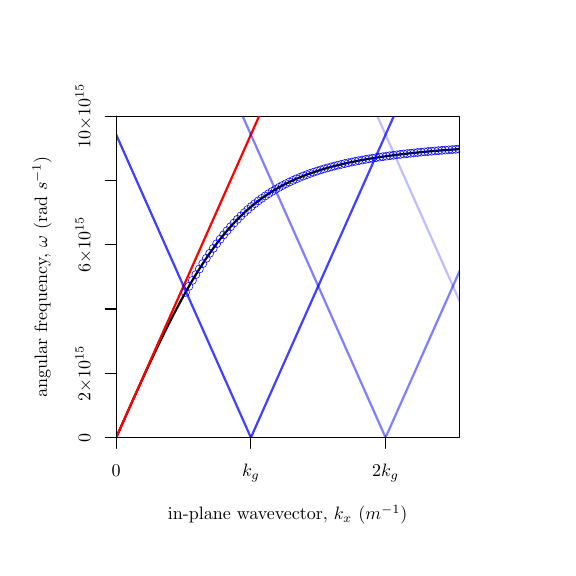
\begin{tikzpicture}[x=1pt,y=1pt,scale=0.65, every node/.style={transform shape}]
\definecolor[named]{fillColor}{rgb}{1.00,1.00,1.00}
\path[use as bounding box,fill=fillColor,fill opacity=0.00] (0,0) rectangle (289.08,289.08);
\begin{scope}
\path[clip] (  0.00,  0.00) rectangle (289.08,289.08);
\definecolor[named]{drawColor}{rgb}{0.00,0.00,0.00}

\path[draw=drawColor,line width= 0.4pt,line join=round,line cap=round] ( 49.20, 61.20) --
	(239.88, 61.20) --
	(239.88,239.88) --
	( 49.20,239.88) --
	( 49.20, 61.20);
\end{scope}
\begin{scope}
\path[clip] (  0.00,  0.00) rectangle (289.08,289.08);
\definecolor[named]{drawColor}{rgb}{0.00,0.00,0.00}

\node[text=drawColor,anchor=base,inner sep=0pt, outer sep=0pt, scale=  1.00] at (144.54, 15.60) {in-plane wavevector, $k_x$ ($m^{-1}$)};

\node[text=drawColor,rotate= 90.00,anchor=base,inner sep=0pt, outer sep=0pt, scale=  1.00] at ( 10.80,150.54) {angular frequency, $\omega$ (rad $s^{-1}$)};
\end{scope}
\begin{scope}
\path[clip] ( 49.20, 61.20) rectangle (239.88,239.88);
\definecolor[named]{drawColor}{rgb}{0.00,0.00,0.00}

\path[draw=drawColor,line width= 0.8pt,line join=round,line cap=round] ( 49.20, 61.20) --
	( 51.13, 65.53) --
	( 53.05, 69.86) --
	( 54.98, 74.18) --
	( 56.90, 78.48) --
	( 58.83, 82.77) --
	( 60.76, 87.03) --
	( 62.68, 91.27) --
	( 64.61, 95.48) --
	( 66.53, 99.65) --
	( 68.46,103.78) --
	( 70.39,107.87) --
	( 72.31,111.90) --
	( 74.24,115.89) --
	( 76.16,119.81) --
	( 78.09,123.68) --
	( 80.02,127.47) --
	( 81.94,131.19) --
	( 83.87,134.84) --
	( 85.80,138.40) --
	( 87.72,141.89) --
	( 89.65,145.28) --
	( 91.57,148.59) --
	( 93.50,151.80) --
	( 95.43,154.91) --
	( 97.35,157.93) --
	( 99.28,160.84) --
	(101.20,163.65) --
	(103.13,166.37) --
	(105.06,168.97) --
	(106.98,171.48) --
	(108.91,173.89) --
	(110.83,176.19) --
	(112.76,178.39) --
	(114.69,180.50) --
	(116.61,182.51) --
	(118.54,184.43) --
	(120.46,186.26) --
	(122.39,188.00) --
	(124.32,189.66) --
	(126.24,191.24) --
	(128.17,192.74) --
	(130.09,194.16) --
	(132.02,195.52) --
	(133.95,196.80) --
	(135.87,198.03) --
	(137.80,199.19) --
	(139.72,200.29) --
	(141.65,201.34) --
	(143.58,202.34) --
	(145.50,203.28) --
	(147.43,204.18) --
	(149.36,205.04) --
	(151.28,205.86) --
	(153.21,206.63) --
	(155.13,207.37) --
	(157.06,208.07) --
	(158.99,208.74) --
	(160.91,209.38) --
	(162.84,209.99) --
	(164.76,210.57) --
	(166.69,211.13) --
	(168.62,211.66) --
	(170.54,212.16) --
	(172.47,212.65) --
	(174.39,213.11) --
	(176.32,213.55) --
	(178.25,213.98) --
	(180.17,214.38) --
	(182.10,214.77) --
	(184.02,215.15) --
	(185.95,215.50) --
	(187.88,215.85) --
	(189.80,216.18) --
	(191.73,216.49) --
	(193.65,216.80) --
	(195.58,217.09) --
	(197.51,217.37) --
	(199.43,217.64) --
	(201.36,217.90) --
	(203.28,218.16) --
	(205.21,218.40) --
	(207.14,218.63) --
	(209.06,218.86) --
	(210.99,219.07) --
	(212.92,219.28) --
	(214.84,219.49) --
	(216.77,219.68) --
	(218.69,219.87) --
	(220.62,220.05) --
	(222.55,220.23) --
	(224.47,220.40) --
	(226.40,220.56) --
	(228.32,220.72) --
	(230.25,220.88) --
	(232.18,221.03) --
	(234.10,221.17) --
	(236.03,221.31) --
	(237.95,221.45) --
	(239.88,221.58);
\definecolor[named]{drawColor}{rgb}{1.00,0.00,0.00}

\path[draw=drawColor,line width= 0.8pt,line join=round,line cap=round] ( 49.20, 61.20) --
	( 51.13, 65.53) --
	( 53.05, 69.86) --
	( 54.98, 74.19) --
	( 56.90, 78.53) --
	( 58.83, 82.86) --
	( 60.76, 87.19) --
	( 62.68, 91.52) --
	( 64.61, 95.85) --
	( 66.53,100.18) --
	( 68.46,104.52) --
	( 70.39,108.85) --
	( 72.31,113.18) --
	( 74.24,117.51) --
	( 76.16,121.84) --
	( 78.09,126.17) --
	( 80.02,130.51) --
	( 81.94,134.84) --
	( 83.87,139.17) --
	( 85.80,143.50) --
	( 87.72,147.83) --
	( 89.65,152.16) --
	( 91.57,156.50) --
	( 93.50,160.83) --
	( 95.43,165.16) --
	( 97.35,169.49) --
	( 99.28,173.82) --
	(101.20,178.15) --
	(103.13,182.49) --
	(105.06,186.82) --
	(106.98,191.15) --
	(108.91,195.48) --
	(110.83,199.81) --
	(112.76,204.14) --
	(114.69,208.48) --
	(116.61,212.81) --
	(118.54,217.14) --
	(120.46,221.47) --
	(122.39,225.80) --
	(124.32,230.13) --
	(126.24,234.47) --
	(128.17,238.80) --
	(130.09,243.13) --
	(132.02,247.46) --
	(133.95,251.79) --
	(135.87,256.12) --
	(137.80,260.46) --
	(139.72,264.79) --
	(141.65,269.12) --
	(143.58,273.45) --
	(145.50,277.78) --
	(147.43,282.11) --
	(149.36,286.45) --
	(150.53,289.08);
\definecolor[named]{drawColor}{rgb}{0.00,0.00,1.00}

\path[draw=drawColor,draw opacity=0.75,line width= 0.8pt,line join=round,line cap=round] (124.08, 61.20) --
	(126.01, 65.53) --
	(127.93, 69.86) --
	(129.86, 74.19) --
	(131.78, 78.53) --
	(133.71, 82.86) --
	(135.64, 87.19) --
	(137.56, 91.52) --
	(139.49, 95.85) --
	(141.41,100.18) --
	(143.34,104.52) --
	(145.27,108.85) --
	(147.19,113.18) --
	(149.12,117.51) --
	(151.04,121.84) --
	(152.97,126.17) --
	(154.90,130.51) --
	(156.82,134.84) --
	(158.75,139.17) --
	(160.68,143.50) --
	(162.60,147.83) --
	(164.53,152.16) --
	(166.45,156.50) --
	(168.38,160.83) --
	(170.31,165.16) --
	(172.23,169.49) --
	(174.16,173.82) --
	(176.08,178.15) --
	(178.01,182.49) --
	(179.94,186.82) --
	(181.86,191.15) --
	(183.79,195.48) --
	(185.71,199.81) --
	(187.64,204.14) --
	(189.57,208.48) --
	(191.49,212.81) --
	(193.42,217.14) --
	(195.34,221.47) --
	(197.27,225.80) --
	(199.20,230.13) --
	(201.12,234.47) --
	(203.05,238.80) --
	(204.97,243.13) --
	(206.90,247.46) --
	(208.83,251.79) --
	(210.75,256.12) --
	(212.68,260.46) --
	(214.60,264.79) --
	(216.53,269.12) --
	(218.46,273.45) --
	(220.38,277.78) --
	(222.31,282.11) --
	(224.24,286.45) --
	(225.41,289.08);

\path[draw=drawColor,draw opacity=0.75,line width= 0.8pt,line join=round,line cap=round] (124.08, 61.20) --
	(122.15, 65.53) --
	(120.23, 69.86) --
	(118.30, 74.19) --
	(116.38, 78.53) --
	(114.45, 82.86) --
	(112.52, 87.19) --
	(110.60, 91.52) --
	(108.67, 95.85) --
	(106.75,100.18) --
	(104.82,104.52) --
	(102.89,108.85) --
	(100.97,113.18) --
	( 99.04,117.51) --
	( 97.12,121.84) --
	( 95.19,126.17) --
	( 93.26,130.51) --
	( 91.34,134.84) --
	( 89.41,139.17) --
	( 87.48,143.50) --
	( 85.56,147.83) --
	( 83.63,152.16) --
	( 81.71,156.50) --
	( 79.78,160.83) --
	( 77.85,165.16) --
	( 75.93,169.49) --
	( 74.00,173.82) --
	( 72.08,178.15) --
	( 70.15,182.49) --
	( 68.22,186.82) --
	( 66.30,191.15) --
	( 64.37,195.48) --
	( 62.45,199.81) --
	( 60.52,204.14) --
	( 58.59,208.48) --
	( 56.67,212.81) --
	( 54.74,217.14) --
	( 52.82,221.47) --
	( 50.89,225.80) --
	( 48.96,230.13) --
	( 47.04,234.47) --
	( 45.11,238.80) --
	( 43.19,243.13) --
	( 41.26,247.46) --
	( 39.33,251.79) --
	( 37.41,256.12) --
	( 35.48,260.46) --
	( 33.56,264.79) --
	( 31.63,269.12) --
	( 29.70,273.45) --
	( 27.78,277.78) --
	( 25.85,282.11) --
	( 23.92,286.45) --
	( 22.75,289.08);
\definecolor[named]{drawColor}{rgb}{0.00,0.00,1.00}

\path[draw=drawColor,draw opacity=0.50,line width= 0.8pt,line join=round,line cap=round] (198.96, 61.20) --
	(200.89, 65.53) --
	(202.81, 69.86) --
	(204.74, 74.19) --
	(206.66, 78.53) --
	(208.59, 82.86) --
	(210.52, 87.19) --
	(212.44, 91.52) --
	(214.37, 95.85) --
	(216.29,100.18) --
	(218.22,104.52) --
	(220.15,108.85) --
	(222.07,113.18) --
	(224.00,117.51) --
	(225.92,121.84) --
	(227.85,126.17) --
	(229.78,130.51) --
	(231.70,134.84) --
	(233.63,139.17) --
	(235.55,143.50) --
	(237.48,147.83) --
	(239.41,152.16) --
	(241.33,156.50) --
	(243.26,160.83) --
	(245.19,165.16) --
	(247.11,169.49) --
	(249.04,173.82) --
	(250.96,178.15) --
	(252.89,182.49) --
	(254.82,186.82) --
	(256.74,191.15) --
	(258.67,195.48) --
	(260.59,199.81) --
	(262.52,204.14) --
	(264.45,208.48) --
	(266.37,212.81) --
	(268.30,217.14) --
	(270.22,221.47) --
	(272.15,225.80) --
	(274.08,230.13) --
	(276.00,234.47) --
	(277.93,238.80) --
	(279.85,243.13) --
	(281.78,247.46) --
	(283.71,251.79) --
	(285.63,256.12) --
	(287.56,260.46) --
	(289.08,263.88);

\path[draw=drawColor,draw opacity=0.50,line width= 0.8pt,line join=round,line cap=round] (198.96, 61.20) --
	(197.03, 65.53) --
	(195.11, 69.86) --
	(193.18, 74.19) --
	(191.26, 78.53) --
	(189.33, 82.86) --
	(187.40, 87.19) --
	(185.48, 91.52) --
	(183.55, 95.85) --
	(181.63,100.18) --
	(179.70,104.52) --
	(177.77,108.85) --
	(175.85,113.18) --
	(173.92,117.51) --
	(171.99,121.84) --
	(170.07,126.17) --
	(168.14,130.51) --
	(166.22,134.84) --
	(164.29,139.17) --
	(162.36,143.50) --
	(160.44,147.83) --
	(158.51,152.16) --
	(156.59,156.50) --
	(154.66,160.83) --
	(152.73,165.16) --
	(150.81,169.49) --
	(148.88,173.82) --
	(146.96,178.15) --
	(145.03,182.49) --
	(143.10,186.82) --
	(141.18,191.15) --
	(139.25,195.48) --
	(137.33,199.81) --
	(135.40,204.14) --
	(133.47,208.48) --
	(131.55,212.81) --
	(129.62,217.14) --
	(127.70,221.47) --
	(125.77,225.80) --
	(123.84,230.13) --
	(121.92,234.47) --
	(119.99,238.80) --
	(118.07,243.13) --
	(116.14,247.46) --
	(114.21,251.79) --
	(112.29,256.12) --
	(110.36,260.46) --
	(108.43,264.79) --
	(106.51,269.12) --
	(104.58,273.45) --
	(102.66,277.78) --
	(100.73,282.11) --
	( 98.80,286.45) --
	( 97.63,289.08);
\definecolor[named]{drawColor}{rgb}{0.00,0.00,1.00}

\path[draw=drawColor,draw opacity=0.25,line width= 0.8pt,line join=round,line cap=round] (273.84, 61.20) --
	(275.77, 65.53) --
	(277.69, 69.86) --
	(279.62, 74.19) --
	(281.54, 78.53) --
	(283.47, 82.86) --
	(285.40, 87.19) --
	(287.32, 91.52) --
	(289.08, 95.48);

\path[draw=drawColor,draw opacity=0.25,line width= 0.8pt,line join=round,line cap=round] (273.84, 61.20) --
	(271.91, 65.53) --
	(269.99, 69.86) --
	(268.06, 74.19) --
	(266.14, 78.53) --
	(264.21, 82.86) --
	(262.28, 87.19) --
	(260.36, 91.52) --
	(258.43, 95.85) --
	(256.51,100.18) --
	(254.58,104.52) --
	(252.65,108.85) --
	(250.73,113.18) --
	(248.80,117.51) --
	(246.87,121.84) --
	(244.95,126.17) --
	(243.02,130.51) --
	(241.10,134.84) --
	(239.17,139.17) --
	(237.24,143.50) --
	(235.32,147.83) --
	(233.39,152.16) --
	(231.47,156.50) --
	(229.54,160.83) --
	(227.61,165.16) --
	(225.69,169.49) --
	(223.76,173.82) --
	(221.84,178.15) --
	(219.91,182.49) --
	(217.98,186.82) --
	(216.06,191.15) --
	(214.13,195.48) --
	(212.21,199.81) --
	(210.28,204.14) --
	(208.35,208.48) --
	(206.43,212.81) --
	(204.50,217.14) --
	(202.58,221.47) --
	(200.65,225.80) --
	(198.72,230.13) --
	(196.80,234.47) --
	(194.87,238.80) --
	(192.95,243.13) --
	(191.02,247.46) --
	(189.09,251.79) --
	(187.17,256.12) --
	(185.24,260.46) --
	(183.31,264.79) --
	(181.39,269.12) --
	(179.46,273.45) --
	(177.54,277.78) --
	(175.61,282.11) --
	(173.68,286.45) --
	(172.51,289.08);
\definecolor[named]{drawColor}{rgb}{0.00,0.00,1.00}

\path[draw=drawColor,line width= 0.2pt,line join=round,line cap=round] ( 87.72,141.89) circle (  2.25);

\path[draw=drawColor,line width= 0.2pt,line join=round,line cap=round] ( 89.65,145.28) circle (  2.25);

\path[draw=drawColor,line width= 0.2pt,line join=round,line cap=round] ( 91.57,148.59) circle (  2.25);

\path[draw=drawColor,line width= 0.2pt,line join=round,line cap=round] ( 93.50,151.80) circle (  2.25);

\path[draw=drawColor,line width= 0.2pt,line join=round,line cap=round] ( 95.43,154.91) circle (  2.25);

\path[draw=drawColor,line width= 0.2pt,line join=round,line cap=round] ( 97.35,157.93) circle (  2.25);

\path[draw=drawColor,line width= 0.2pt,line join=round,line cap=round] ( 99.28,160.84) circle (  2.25);

\path[draw=drawColor,line width= 0.2pt,line join=round,line cap=round] (101.20,163.65) circle (  2.25);

\path[draw=drawColor,line width= 0.2pt,line join=round,line cap=round] (103.13,166.37) circle (  2.25);

\path[draw=drawColor,line width= 0.2pt,line join=round,line cap=round] (105.06,168.97) circle (  2.25);

\path[draw=drawColor,line width= 0.2pt,line join=round,line cap=round] (106.98,171.48) circle (  2.25);

\path[draw=drawColor,line width= 0.2pt,line join=round,line cap=round] (108.91,173.89) circle (  2.25);

\path[draw=drawColor,line width= 0.2pt,line join=round,line cap=round] (110.83,176.19) circle (  2.25);

\path[draw=drawColor,line width= 0.2pt,line join=round,line cap=round] (112.76,178.39) circle (  2.25);

\path[draw=drawColor,line width= 0.2pt,line join=round,line cap=round] (114.69,180.50) circle (  2.25);

\path[draw=drawColor,line width= 0.2pt,line join=round,line cap=round] (116.61,182.51) circle (  2.25);

\path[draw=drawColor,line width= 0.2pt,line join=round,line cap=round] (118.54,184.43) circle (  2.25);

\path[draw=drawColor,line width= 0.2pt,line join=round,line cap=round] (120.46,186.26) circle (  2.25);

\path[draw=drawColor,line width= 0.2pt,line join=round,line cap=round] (122.39,188.00) circle (  2.25);

\path[draw=drawColor,line width= 0.2pt,line join=round,line cap=round] (124.32,189.66) circle (  2.25);

\path[draw=drawColor,line width= 0.2pt,line join=round,line cap=round] (126.24,191.24) circle (  2.25);

\path[draw=drawColor,line width= 0.2pt,line join=round,line cap=round] (128.17,192.74) circle (  2.25);

\path[draw=drawColor,line width= 0.2pt,line join=round,line cap=round] (130.09,194.16) circle (  2.25);

\path[draw=drawColor,line width= 0.2pt,line join=round,line cap=round] (132.02,195.52) circle (  2.25);

\path[draw=drawColor,line width= 0.2pt,line join=round,line cap=round] (133.95,196.80) circle (  2.25);

\path[draw=drawColor,line width= 0.2pt,line join=round,line cap=round] (135.87,198.03) circle (  2.25);

\path[draw=drawColor,line width= 0.2pt,line join=round,line cap=round] (137.80,199.19) circle (  2.25);

\path[draw=drawColor,line width= 0.2pt,line join=round,line cap=round] (139.72,200.29) circle (  2.25);

\path[draw=drawColor,line width= 0.2pt,line join=round,line cap=round] (141.65,201.34) circle (  2.25);

\path[draw=drawColor,line width= 0.2pt,line join=round,line cap=round] (143.58,202.34) circle (  2.25);

\path[draw=drawColor,line width= 0.2pt,line join=round,line cap=round] (145.50,203.28) circle (  2.25);

\path[draw=drawColor,line width= 0.2pt,line join=round,line cap=round] (147.43,204.18) circle (  2.25);

\path[draw=drawColor,line width= 0.2pt,line join=round,line cap=round] (149.36,205.04) circle (  2.25);

\path[draw=drawColor,line width= 0.2pt,line join=round,line cap=round] (151.28,205.86) circle (  2.25);

\path[draw=drawColor,line width= 0.2pt,line join=round,line cap=round] (153.21,206.63) circle (  2.25);

\path[draw=drawColor,line width= 0.2pt,line join=round,line cap=round] (155.13,207.37) circle (  2.25);

\path[draw=drawColor,line width= 0.2pt,line join=round,line cap=round] (157.06,208.07) circle (  2.25);

\path[draw=drawColor,line width= 0.2pt,line join=round,line cap=round] (158.99,208.74) circle (  2.25);

\path[draw=drawColor,line width= 0.2pt,line join=round,line cap=round] (160.91,209.38) circle (  2.25);

\path[draw=drawColor,line width= 0.2pt,line join=round,line cap=round] (162.84,209.99) circle (  2.25);

\path[draw=drawColor,line width= 0.2pt,line join=round,line cap=round] (164.76,210.57) circle (  2.25);

\path[draw=drawColor,line width= 0.2pt,line join=round,line cap=round] (166.69,211.13) circle (  2.25);

\path[draw=drawColor,line width= 0.2pt,line join=round,line cap=round] (168.62,211.66) circle (  2.25);

\path[draw=drawColor,line width= 0.2pt,line join=round,line cap=round] (170.54,212.16) circle (  2.25);

\path[draw=drawColor,line width= 0.2pt,line join=round,line cap=round] (172.47,212.65) circle (  2.25);

\path[draw=drawColor,line width= 0.2pt,line join=round,line cap=round] (174.39,213.11) circle (  2.25);

\path[draw=drawColor,line width= 0.2pt,line join=round,line cap=round] (176.32,213.55) circle (  2.25);

\path[draw=drawColor,line width= 0.2pt,line join=round,line cap=round] (178.25,213.98) circle (  2.25);

\path[draw=drawColor,line width= 0.2pt,line join=round,line cap=round] (180.17,214.38) circle (  2.25);

\path[draw=drawColor,line width= 0.2pt,line join=round,line cap=round] (182.10,214.77) circle (  2.25);

\path[draw=drawColor,line width= 0.2pt,line join=round,line cap=round] (184.02,215.15) circle (  2.25);

\path[draw=drawColor,line width= 0.2pt,line join=round,line cap=round] (185.95,215.50) circle (  2.25);

\path[draw=drawColor,line width= 0.2pt,line join=round,line cap=round] (187.88,215.85) circle (  2.25);

\path[draw=drawColor,line width= 0.2pt,line join=round,line cap=round] (189.80,216.18) circle (  2.25);

\path[draw=drawColor,line width= 0.2pt,line join=round,line cap=round] (191.73,216.49) circle (  2.25);

\path[draw=drawColor,line width= 0.2pt,line join=round,line cap=round] (193.65,216.80) circle (  2.25);

\path[draw=drawColor,line width= 0.2pt,line join=round,line cap=round] (195.58,217.09) circle (  2.25);

\path[draw=drawColor,line width= 0.2pt,line join=round,line cap=round] (197.51,217.37) circle (  2.25);

\path[draw=drawColor,line width= 0.2pt,line join=round,line cap=round] (199.43,217.64) circle (  2.25);

\path[draw=drawColor,line width= 0.2pt,line join=round,line cap=round] (201.36,217.90) circle (  2.25);

\path[draw=drawColor,line width= 0.2pt,line join=round,line cap=round] (203.28,218.16) circle (  2.25);

\path[draw=drawColor,line width= 0.2pt,line join=round,line cap=round] (205.21,218.40) circle (  2.25);

\path[draw=drawColor,line width= 0.2pt,line join=round,line cap=round] (207.14,218.63) circle (  2.25);

\path[draw=drawColor,line width= 0.2pt,line join=round,line cap=round] (209.06,218.86) circle (  2.25);

\path[draw=drawColor,line width= 0.2pt,line join=round,line cap=round] (210.99,219.07) circle (  2.25);

\path[draw=drawColor,line width= 0.2pt,line join=round,line cap=round] (212.92,219.28) circle (  2.25);

\path[draw=drawColor,line width= 0.2pt,line join=round,line cap=round] (214.84,219.49) circle (  2.25);

\path[draw=drawColor,line width= 0.2pt,line join=round,line cap=round] (216.77,219.68) circle (  2.25);

\path[draw=drawColor,line width= 0.2pt,line join=round,line cap=round] (218.69,219.87) circle (  2.25);

\path[draw=drawColor,line width= 0.2pt,line join=round,line cap=round] (220.62,220.05) circle (  2.25);

\path[draw=drawColor,line width= 0.2pt,line join=round,line cap=round] (222.55,220.23) circle (  2.25);

\path[draw=drawColor,line width= 0.2pt,line join=round,line cap=round] (224.47,220.40) circle (  2.25);

\path[draw=drawColor,line width= 0.2pt,line join=round,line cap=round] (226.40,220.56) circle (  2.25);

\path[draw=drawColor,line width= 0.2pt,line join=round,line cap=round] (228.32,220.72) circle (  2.25);

\path[draw=drawColor,line width= 0.2pt,line join=round,line cap=round] (230.25,220.88) circle (  2.25);

\path[draw=drawColor,line width= 0.2pt,line join=round,line cap=round] (232.18,221.03) circle (  2.25);

\path[draw=drawColor,line width= 0.2pt,line join=round,line cap=round] (234.10,221.17) circle (  2.25);

\path[draw=drawColor,line width= 0.2pt,line join=round,line cap=round] (236.03,221.31) circle (  2.25);

\path[draw=drawColor,line width= 0.2pt,line join=round,line cap=round] (237.95,221.45) circle (  2.25);

\path[draw=drawColor,line width= 0.2pt,line join=round,line cap=round] (239.88,221.58) circle (  2.25);
\end{scope}
\begin{scope}
\path[clip] (  0.00,  0.00) rectangle (289.08,289.08);
\definecolor[named]{drawColor}{rgb}{0.00,0.00,0.00}

\path[draw=drawColor,line width= 0.4pt,line join=round,line cap=round] ( 49.20, 61.20) -- (198.96, 61.20);

\path[draw=drawColor,line width= 0.4pt,line join=round,line cap=round] ( 49.20, 61.20) -- ( 49.20, 55.20);

\path[draw=drawColor,line width= 0.4pt,line join=round,line cap=round] (124.08, 61.20) -- (124.08, 55.20);

\path[draw=drawColor,line width= 0.4pt,line join=round,line cap=round] (198.96, 61.20) -- (198.96, 55.20);

\node[text=drawColor,anchor=base,inner sep=0pt, outer sep=0pt, scale=  1.00] at ( 49.20, 39.60) {0};

\node[text=drawColor,anchor=base,inner sep=0pt, outer sep=0pt, scale=  1.00] at (124.08, 39.60) {$k_g$};

\node[text=drawColor,anchor=base,inner sep=0pt, outer sep=0pt, scale=  1.00] at (198.96, 39.60) {$2k_g$};

\path[draw=drawColor,line width= 0.4pt,line join=round,line cap=round] ( 49.20, 61.20) -- ( 49.20,239.88);

\path[draw=drawColor,line width= 0.4pt,line join=round,line cap=round] ( 49.20, 61.20) -- ( 43.20, 61.20);

\path[draw=drawColor,line width= 0.4pt,line join=round,line cap=round] ( 49.20, 96.94) -- ( 43.20, 96.94);

\path[draw=drawColor,line width= 0.4pt,line join=round,line cap=round] ( 49.20,132.67) -- ( 43.20,132.67);

\path[draw=drawColor,line width= 0.4pt,line join=round,line cap=round] ( 49.20,168.41) -- ( 43.20,168.41);

\path[draw=drawColor,line width= 0.4pt,line join=round,line cap=round] ( 49.20,204.14) -- ( 43.20,204.14);

\path[draw=drawColor,line width= 0.4pt,line join=round,line cap=round] ( 49.20,239.88) -- ( 43.20,239.88);

\node[text=drawColor,rotate= 90.00,anchor=base,inner sep=0pt, outer sep=0pt, scale=  1.00] at ( 34.80, 61.20) {0};

\node[text=drawColor,rotate= 90.00,anchor=base,inner sep=0pt, outer sep=0pt, scale=  1.00] at ( 34.80, 96.94) {2$\times 10^{15}$};

\node[text=drawColor,rotate= 90.00,anchor=base,inner sep=0pt, outer sep=0pt, scale=  1.00] at ( 34.80,168.41) {6$\times 10^{15}$};

\node[text=drawColor,rotate= 90.00,anchor=base,inner sep=0pt, outer sep=0pt, scale=  1.00] at ( 34.80,239.88) {10$\times 10^{15}$};
\end{scope}
\end{tikzpicture}
\label{fig:diffractive-couplingA}
}
		\subfigure[]{
		\centering% Created by tikzDevice version 0.6.2-92-0ad2792 on 2012-09-26 20:32:08
% !TEX encoding = UTF-8 Unicode
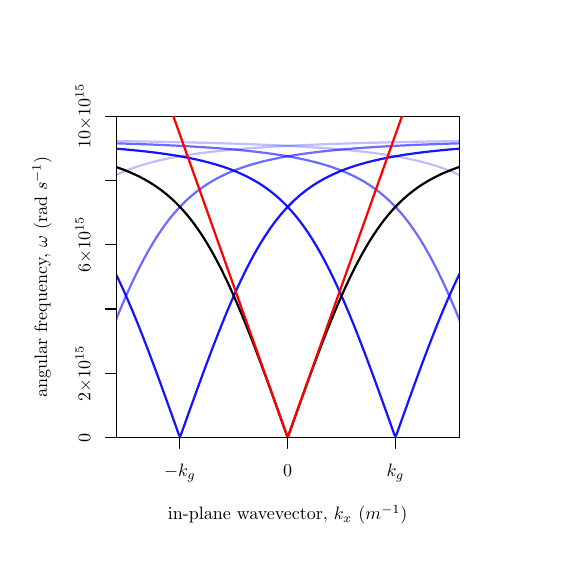
\begin{tikzpicture}[x=1pt,y=1pt,scale=0.65, every node/.style={transform shape}]
\definecolor[named]{fillColor}{rgb}{1.00,1.00,1.00}
\path[use as bounding box,fill=fillColor,fill opacity=0.00] (0,0) rectangle (289.08,289.08);
\begin{scope}
\path[clip] (  0.00,  0.00) rectangle (289.08,289.08);
\definecolor[named]{drawColor}{rgb}{0.00,0.00,0.00}

\path[draw=drawColor,line width= 0.4pt,line join=round,line cap=round] ( 49.20, 61.20) --
	(239.88, 61.20) --
	(239.88,239.88) --
	( 49.20,239.88) --
	( 49.20, 61.20);
\end{scope}
\begin{scope}
\path[clip] (  0.00,  0.00) rectangle (289.08,289.08);
\definecolor[named]{drawColor}{rgb}{0.00,0.00,0.00}

\node[text=drawColor,anchor=base,inner sep=0pt, outer sep=0pt, scale=  1.00] at (144.54, 15.60) {in-plane wavevector, $k_x$ ($m^{-1}$)};

\node[text=drawColor,rotate= 90.00,anchor=base,inner sep=0pt, outer sep=0pt, scale=  1.00] at ( 10.80,150.54) {angular frequency, $\omega$ (rad $s^{-1}$)};
\end{scope}
\begin{scope}
\path[clip] ( 49.20, 61.20) rectangle (239.88,239.88);
\definecolor[named]{drawColor}{rgb}{0.00,0.00,1.00}

\path[draw=drawColor,draw opacity=0.25,line width= 0.8pt,line join=round,line cap=round] (  0.00,151.24) --
	(  0.30,151.87) --
	(  1.06,153.42) --
	(  1.83,154.95) --
	(  2.59,156.45) --
	(  3.35,157.93) --
	(  4.12,159.39) --
	(  4.88,160.82) --
	(  5.64,162.23) --
	(  6.40,163.61) --
	(  7.17,164.96) --
	(  7.93,166.29) --
	(  8.69,167.60) --
	(  9.46,168.88) --
	( 10.22,170.14) --
	( 10.98,171.37) --
	( 11.74,172.57) --
	( 12.51,173.75) --
	( 13.27,174.91) --
	( 14.03,176.04) --
	( 14.80,177.15) --
	( 15.56,178.23) --
	( 16.32,179.29) --
	( 17.09,180.32) --
	( 17.85,181.34) --
	( 18.61,182.32) --
	( 19.37,183.29) --
	( 20.14,184.23) --
	( 20.90,185.16) --
	( 21.66,186.05) --
	( 22.43,186.93) --
	( 23.19,187.79) --
	( 23.95,188.63) --
	( 24.71,189.44) --
	( 25.48,190.24) --
	( 26.24,191.01) --
	( 27.00,191.77) --
	( 27.77,192.51) --
	( 28.53,193.23) --
	( 29.29,193.93) --
	( 30.05,194.62) --
	( 30.82,195.29) --
	( 31.58,195.94) --
	( 32.34,196.57) --
	( 33.11,197.19) --
	( 33.87,197.80) --
	( 34.63,198.38) --
	( 35.39,198.96) --
	( 36.16,199.52) --
	( 36.92,200.06) --
	( 37.68,200.59) --
	( 38.45,201.11) --
	( 39.21,201.62) --
	( 39.97,202.11) --
	( 40.73,202.59) --
	( 41.50,203.06) --
	( 42.26,203.52) --
	( 43.02,203.96) --
	( 43.79,204.40) --
	( 44.55,204.82) --
	( 45.31,205.23) --
	( 46.07,205.64) --
	( 46.84,206.03) --
	( 47.60,206.42) --
	( 48.36,206.79) --
	( 49.13,207.16) --
	( 49.89,207.52) --
	( 50.65,207.86) --
	( 51.41,208.20) --
	( 52.18,208.54) --
	( 52.94,208.86) --
	( 53.70,209.18) --
	( 54.47,209.49) --
	( 55.23,209.79) --
	( 55.99,210.09) --
	( 56.75,210.38) --
	( 57.52,210.66) --
	( 58.28,210.93) --
	( 59.04,211.20) --
	( 59.81,211.47) --
	( 60.57,211.73) --
	( 61.33,211.98) --
	( 62.09,212.22) --
	( 62.86,212.47) --
	( 63.62,212.70) --
	( 64.38,212.93) --
	( 65.15,213.16) --
	( 65.91,213.38) --
	( 66.67,213.59) --
	( 67.43,213.81) --
	( 68.20,214.01) --
	( 68.96,214.21) --
	( 69.72,214.41) --
	( 70.49,214.61) --
	( 71.25,214.80) --
	( 72.01,214.98) --
	( 72.77,215.17) --
	( 73.54,215.34) --
	( 74.30,215.52) --
	( 75.06,215.69) --
	( 75.83,215.86) --
	( 76.59,216.02) --
	( 77.35,216.19) --
	( 78.11,216.34) --
	( 78.88,216.50) --
	( 79.64,216.65) --
	( 80.40,216.80) --
	( 81.17,216.95) --
	( 81.93,217.09) --
	( 82.69,217.23) --
	( 83.46,217.37) --
	( 84.22,217.51) --
	( 84.98,217.64) --
	( 85.74,217.77) --
	( 86.51,217.90) --
	( 87.27,218.02) --
	( 88.03,218.15) --
	( 88.80,218.27) --
	( 89.56,218.39) --
	( 90.32,218.50) --
	( 91.08,218.62) --
	( 91.85,218.73) --
	( 92.61,218.84) --
	( 93.37,218.95) --
	( 94.14,219.06) --
	( 94.90,219.16) --
	( 95.66,219.26) --
	( 96.42,219.37) --
	( 97.19,219.47) --
	( 97.95,219.56) --
	( 98.71,219.66) --
	( 99.48,219.75) --
	(100.24,219.85) --
	(101.00,219.94) --
	(101.76,220.03) --
	(102.53,220.12) --
	(103.29,220.20) --
	(104.05,220.29) --
	(104.82,220.37) --
	(105.58,220.46) --
	(106.34,220.54) --
	(107.10,220.62) --
	(107.87,220.70) --
	(108.63,220.78) --
	(109.39,220.85) --
	(110.16,220.93) --
	(110.92,221.00) --
	(111.68,221.07) --
	(112.44,221.15) --
	(113.21,221.22) --
	(113.97,221.29) --
	(114.73,221.35) --
	(115.50,221.42) --
	(116.26,221.49) --
	(117.02,221.55) --
	(117.78,221.62) --
	(118.55,221.68) --
	(119.31,221.74) --
	(120.07,221.81) --
	(120.84,221.87) --
	(121.60,221.93) --
	(122.36,221.99) --
	(123.12,222.04) --
	(123.89,222.10) --
	(124.65,222.16) --
	(125.41,222.21) --
	(126.18,222.27) --
	(126.94,222.32) --
	(127.70,222.37) --
	(128.46,222.43) --
	(129.23,222.48) --
	(129.99,222.53) --
	(130.75,222.58) --
	(131.52,222.63) --
	(132.28,222.68) --
	(133.04,222.73) --
	(133.80,222.78) --
	(134.57,222.82) --
	(135.33,222.87) --
	(136.09,222.91) --
	(136.86,222.96) --
	(137.62,223.00) --
	(138.38,223.05) --
	(139.14,223.09) --
	(139.91,223.13) --
	(140.67,223.18) --
	(141.43,223.22) --
	(142.20,223.26) --
	(142.96,223.30) --
	(143.72,223.34) --
	(144.48,223.38) --
	(145.25,223.42) --
	(146.01,223.46) --
	(146.77,223.50) --
	(147.54,223.53) --
	(148.30,223.57) --
	(149.06,223.61) --
	(149.82,223.64) --
	(150.59,223.68) --
	(151.35,223.71) --
	(152.11,223.75) --
	(152.88,223.78) --
	(153.64,223.82) --
	(154.40,223.85) --
	(155.17,223.89) --
	(155.93,223.92) --
	(156.69,223.95) --
	(157.45,223.98) --
	(158.22,224.01) --
	(158.98,224.05) --
	(159.74,224.08) --
	(160.51,224.11) --
	(161.27,224.14) --
	(162.03,224.17) --
	(162.79,224.20) --
	(163.56,224.23) --
	(164.32,224.25) --
	(165.08,224.28) --
	(165.85,224.31) --
	(166.61,224.34) --
	(167.37,224.37) --
	(168.13,224.39) --
	(168.90,224.42) --
	(169.66,224.45) --
	(170.42,224.47) --
	(171.19,224.50) --
	(171.95,224.53) --
	(172.71,224.55) --
	(173.47,224.58) --
	(174.24,224.60) --
	(175.00,224.63) --
	(175.76,224.65) --
	(176.53,224.67) --
	(177.29,224.70) --
	(178.05,224.72) --
	(178.81,224.75) --
	(179.58,224.77) --
	(180.34,224.79) --
	(181.10,224.81) --
	(181.87,224.84) --
	(182.63,224.86) --
	(183.39,224.88) --
	(184.15,224.90) --
	(184.92,224.92) --
	(185.68,224.94) --
	(186.44,224.97) --
	(187.21,224.99) --
	(187.97,225.01) --
	(188.73,225.03) --
	(189.49,225.05) --
	(190.26,225.07) --
	(191.02,225.09) --
	(191.78,225.11) --
	(192.55,225.13) --
	(193.31,225.14) --
	(194.07,225.16) --
	(194.83,225.18) --
	(195.60,225.20) --
	(196.36,225.22) --
	(197.12,225.24) --
	(197.89,225.26) --
	(198.65,225.27) --
	(199.41,225.29) --
	(200.17,225.31) --
	(200.94,225.33) --
	(201.70,225.34) --
	(202.46,225.36) --
	(203.23,225.38) --
	(203.99,225.39) --
	(204.75,225.41) --
	(205.51,225.43) --
	(206.28,225.44) --
	(207.04,225.46) --
	(207.80,225.47) --
	(208.57,225.49) --
	(209.33,225.51) --
	(210.09,225.52) --
	(210.85,225.54) --
	(211.62,225.55) --
	(212.38,225.57) --
	(213.14,225.58) --
	(213.91,225.60) --
	(214.67,225.61) --
	(215.43,225.63) --
	(216.19,225.64) --
	(216.96,225.65) --
	(217.72,225.67) --
	(218.48,225.68) --
	(219.25,225.70) --
	(220.01,225.71) --
	(220.77,225.72) --
	(221.53,225.74) --
	(222.30,225.75) --
	(223.06,225.76) --
	(223.82,225.78) --
	(224.59,225.79) --
	(225.35,225.80) --
	(226.11,225.81) --
	(226.88,225.83) --
	(227.64,225.84) --
	(228.40,225.85) --
	(229.16,225.86) --
	(229.93,225.88) --
	(230.69,225.89) --
	(231.45,225.90) --
	(232.22,225.91) --
	(232.98,225.92) --
	(233.74,225.94) --
	(234.50,225.95) --
	(235.27,225.96) --
	(236.03,225.97) --
	(236.79,225.98) --
	(237.56,225.99) --
	(238.32,226.00) --
	(239.08,226.02) --
	(239.84,226.03) --
	(240.61,226.04) --
	(241.37,226.05) --
	(242.13,226.06) --
	(242.90,226.07) --
	(243.66,226.08) --
	(244.42,226.09) --
	(245.18,226.10) --
	(245.95,226.11) --
	(246.71,226.12) --
	(247.47,226.13) --
	(248.24,226.14) --
	(249.00,226.15) --
	(249.76,226.16) --
	(250.52,226.17) --
	(251.29,226.18) --
	(252.05,226.19) --
	(252.81,226.20) --
	(253.58,226.21) --
	(254.34,226.22) --
	(255.10,226.23) --
	(255.86,226.24) --
	(256.63,226.24) --
	(257.39,226.25) --
	(258.15,226.26) --
	(258.92,226.27) --
	(259.68,226.28) --
	(260.44,226.29) --
	(261.20,226.30) --
	(261.97,226.31) --
	(262.73,226.32) --
	(263.49,226.32) --
	(264.26,226.33) --
	(265.02,226.34) --
	(265.78,226.35) --
	(266.54,226.36) --
	(267.31,226.37) --
	(268.07,226.37) --
	(268.83,226.38) --
	(269.60,226.39) --
	(270.36,226.40) --
	(271.12,226.41) --
	(271.88,226.41) --
	(272.65,226.42) --
	(273.41,226.43) --
	(274.17,226.44) --
	(274.94,226.44) --
	(275.70,226.45) --
	(276.46,226.46) --
	(277.22,226.47) --
	(277.99,226.47) --
	(278.75,226.48) --
	(279.51,226.49) --
	(280.28,226.50) --
	(281.04,226.50) --
	(281.80,226.51) --
	(282.56,226.52) --
	(283.33,226.52) --
	(284.09,226.53) --
	(284.85,226.54) --
	(285.62,226.54) --
	(286.38,226.55) --
	(287.14,226.56) --
	(287.90,226.57) --
	(288.67,226.57) --
	(289.08,226.58);
\definecolor[named]{drawColor}{rgb}{0.00,0.00,1.00}

\path[draw=drawColor,draw opacity=0.58,line width= 0.8pt,line join=round,line cap=round] (  0.00,127.66) --
	(  0.70,125.94) --
	(  1.46,124.06) --
	(  2.23,122.16) --
	(  2.99,120.24) --
	(  3.75,118.31) --
	(  4.52,116.36) --
	(  5.28,114.40) --
	(  6.04,112.43) --
	(  6.80,110.44) --
	(  7.57,108.43) --
	(  8.33,106.42) --
	(  9.09,104.39) --
	(  9.86,102.36) --
	( 10.62,100.31) --
	( 11.38, 98.25) --
	( 12.14, 96.19) --
	( 12.91, 94.11) --
	( 13.67, 92.03) --
	( 14.43, 89.93) --
	( 15.20, 87.83) --
	( 15.96, 85.73) --
	( 16.72, 83.62) --
	( 17.48, 81.50) --
	( 18.25, 79.37) --
	( 19.01, 77.25) --
	( 19.77, 75.12) --
	( 20.54, 72.98) --
	( 21.30, 70.84) --
	( 22.06, 68.70) --
	( 22.83, 66.56) --
	( 23.59, 64.42) --
	( 24.35, 62.27) --
	( 25.11, 62.27) --
	( 25.88, 64.42) --
	( 26.64, 66.56) --
	( 27.40, 68.70) --
	( 28.17, 70.84) --
	( 28.93, 72.98) --
	( 29.69, 75.12) --
	( 30.45, 77.25) --
	( 31.22, 79.37) --
	( 31.98, 81.50) --
	( 32.74, 83.62) --
	( 33.51, 85.73) --
	( 34.27, 87.83) --
	( 35.03, 89.93) --
	( 35.79, 92.03) --
	( 36.56, 94.11) --
	( 37.32, 96.19) --
	( 38.08, 98.25) --
	( 38.85,100.31) --
	( 39.61,102.36) --
	( 40.37,104.39) --
	( 41.13,106.42) --
	( 41.90,108.43) --
	( 42.66,110.44) --
	( 43.42,112.43) --
	( 44.19,114.40) --
	( 44.95,116.36) --
	( 45.71,118.31) --
	( 46.47,120.24) --
	( 47.24,122.16) --
	( 48.00,124.06) --
	( 48.76,125.94) --
	( 49.53,127.81) --
	( 50.29,129.66) --
	( 51.05,131.49) --
	( 51.81,133.30) --
	( 52.58,135.09) --
	( 53.34,136.87) --
	( 54.10,138.62) --
	( 54.87,140.35) --
	( 55.63,142.06) --
	( 56.39,143.75) --
	( 57.15,145.42) --
	( 57.92,147.07) --
	( 58.68,148.69) --
	( 59.44,150.29) --
	( 60.21,151.87) --
	( 60.97,153.42) --
	( 61.73,154.95) --
	( 62.49,156.45) --
	( 63.26,157.93) --
	( 64.02,159.39) --
	( 64.78,160.82) --
	( 65.55,162.23) --
	( 66.31,163.61) --
	( 67.07,164.96) --
	( 67.83,166.29) --
	( 68.60,167.60) --
	( 69.36,168.88) --
	( 70.12,170.14) --
	( 70.89,171.37) --
	( 71.65,172.57) --
	( 72.41,173.75) --
	( 73.17,174.91) --
	( 73.94,176.04) --
	( 74.70,177.15) --
	( 75.46,178.23) --
	( 76.23,179.29) --
	( 76.99,180.32) --
	( 77.75,181.34) --
	( 78.51,182.32) --
	( 79.28,183.29) --
	( 80.04,184.23) --
	( 80.80,185.16) --
	( 81.57,186.05) --
	( 82.33,186.93) --
	( 83.09,187.79) --
	( 83.85,188.63) --
	( 84.62,189.44) --
	( 85.38,190.24) --
	( 86.14,191.01) --
	( 86.91,191.77) --
	( 87.67,192.51) --
	( 88.43,193.23) --
	( 89.19,193.93) --
	( 89.96,194.62) --
	( 90.72,195.29) --
	( 91.48,195.94) --
	( 92.25,196.57) --
	( 93.01,197.19) --
	( 93.77,197.80) --
	( 94.54,198.38) --
	( 95.30,198.96) --
	( 96.06,199.52) --
	( 96.82,200.06) --
	( 97.59,200.59) --
	( 98.35,201.11) --
	( 99.11,201.62) --
	( 99.88,202.11) --
	(100.64,202.59) --
	(101.40,203.06) --
	(102.16,203.52) --
	(102.93,203.96) --
	(103.69,204.40) --
	(104.45,204.82) --
	(105.22,205.23) --
	(105.98,205.64) --
	(106.74,206.03) --
	(107.50,206.42) --
	(108.27,206.79) --
	(109.03,207.16) --
	(109.79,207.52) --
	(110.56,207.86) --
	(111.32,208.20) --
	(112.08,208.54) --
	(112.84,208.86) --
	(113.61,209.18) --
	(114.37,209.49) --
	(115.13,209.79) --
	(115.90,210.09) --
	(116.66,210.38) --
	(117.42,210.66) --
	(118.18,210.93) --
	(118.95,211.20) --
	(119.71,211.47) --
	(120.47,211.73) --
	(121.24,211.98) --
	(122.00,212.22) --
	(122.76,212.47) --
	(123.52,212.70) --
	(124.29,212.93) --
	(125.05,213.16) --
	(125.81,213.38) --
	(126.58,213.59) --
	(127.34,213.81) --
	(128.10,214.01) --
	(128.86,214.21) --
	(129.63,214.41) --
	(130.39,214.61) --
	(131.15,214.80) --
	(131.92,214.98) --
	(132.68,215.17) --
	(133.44,215.34) --
	(134.20,215.52) --
	(134.97,215.69) --
	(135.73,215.86) --
	(136.49,216.02) --
	(137.26,216.19) --
	(138.02,216.34) --
	(138.78,216.50) --
	(139.54,216.65) --
	(140.31,216.80) --
	(141.07,216.95) --
	(141.83,217.09) --
	(142.60,217.23) --
	(143.36,217.37) --
	(144.12,217.51) --
	(144.88,217.64) --
	(145.65,217.77) --
	(146.41,217.90) --
	(147.17,218.02) --
	(147.94,218.15) --
	(148.70,218.27) --
	(149.46,218.39) --
	(150.22,218.50) --
	(150.99,218.62) --
	(151.75,218.73) --
	(152.51,218.84) --
	(153.28,218.95) --
	(154.04,219.06) --
	(154.80,219.16) --
	(155.56,219.26) --
	(156.33,219.37) --
	(157.09,219.47) --
	(157.85,219.56) --
	(158.62,219.66) --
	(159.38,219.75) --
	(160.14,219.85) --
	(160.90,219.94) --
	(161.67,220.03) --
	(162.43,220.12) --
	(163.19,220.20) --
	(163.96,220.29) --
	(164.72,220.37) --
	(165.48,220.46) --
	(166.25,220.54) --
	(167.01,220.62) --
	(167.77,220.70) --
	(168.53,220.78) --
	(169.30,220.85) --
	(170.06,220.93) --
	(170.82,221.00) --
	(171.59,221.07) --
	(172.35,221.15) --
	(173.11,221.22) --
	(173.87,221.29) --
	(174.64,221.35) --
	(175.40,221.42) --
	(176.16,221.49) --
	(176.93,221.55) --
	(177.69,221.62) --
	(178.45,221.68) --
	(179.21,221.74) --
	(179.98,221.81) --
	(180.74,221.87) --
	(181.50,221.93) --
	(182.27,221.99) --
	(183.03,222.04) --
	(183.79,222.10) --
	(184.55,222.16) --
	(185.32,222.21) --
	(186.08,222.27) --
	(186.84,222.32) --
	(187.61,222.37) --
	(188.37,222.43) --
	(189.13,222.48) --
	(189.89,222.53) --
	(190.66,222.58) --
	(191.42,222.63) --
	(192.18,222.68) --
	(192.95,222.73) --
	(193.71,222.78) --
	(194.47,222.82) --
	(195.23,222.87) --
	(196.00,222.91) --
	(196.76,222.96) --
	(197.52,223.00) --
	(198.29,223.05) --
	(199.05,223.09) --
	(199.81,223.13) --
	(200.57,223.18) --
	(201.34,223.22) --
	(202.10,223.26) --
	(202.86,223.30) --
	(203.63,223.34) --
	(204.39,223.38) --
	(205.15,223.42) --
	(205.91,223.46) --
	(206.68,223.50) --
	(207.44,223.53) --
	(208.20,223.57) --
	(208.97,223.61) --
	(209.73,223.64) --
	(210.49,223.68) --
	(211.25,223.71) --
	(212.02,223.75) --
	(212.78,223.78) --
	(213.54,223.82) --
	(214.31,223.85) --
	(215.07,223.89) --
	(215.83,223.92) --
	(216.59,223.95) --
	(217.36,223.98) --
	(218.12,224.01) --
	(218.88,224.05) --
	(219.65,224.08) --
	(220.41,224.11) --
	(221.17,224.14) --
	(221.93,224.17) --
	(222.70,224.20) --
	(223.46,224.23) --
	(224.22,224.25) --
	(224.99,224.28) --
	(225.75,224.31) --
	(226.51,224.34) --
	(227.27,224.37) --
	(228.04,224.39) --
	(228.80,224.42) --
	(229.56,224.45) --
	(230.33,224.47) --
	(231.09,224.50) --
	(231.85,224.53) --
	(232.61,224.55) --
	(233.38,224.58) --
	(234.14,224.60) --
	(234.90,224.63) --
	(235.67,224.65) --
	(236.43,224.67) --
	(237.19,224.70) --
	(237.96,224.72) --
	(238.72,224.75) --
	(239.48,224.77) --
	(240.24,224.79) --
	(241.01,224.81) --
	(241.77,224.84) --
	(242.53,224.86) --
	(243.30,224.88) --
	(244.06,224.90) --
	(244.82,224.92) --
	(245.58,224.94) --
	(246.35,224.97) --
	(247.11,224.99) --
	(247.87,225.01) --
	(248.64,225.03) --
	(249.40,225.05) --
	(250.16,225.07) --
	(250.92,225.09) --
	(251.69,225.11) --
	(252.45,225.13) --
	(253.21,225.14) --
	(253.98,225.16) --
	(254.74,225.18) --
	(255.50,225.20) --
	(256.26,225.22) --
	(257.03,225.24) --
	(257.79,225.26) --
	(258.55,225.27) --
	(259.32,225.29) --
	(260.08,225.31) --
	(260.84,225.33) --
	(261.60,225.34) --
	(262.37,225.36) --
	(263.13,225.38) --
	(263.89,225.39) --
	(264.66,225.41) --
	(265.42,225.43) --
	(266.18,225.44) --
	(266.94,225.46) --
	(267.71,225.47) --
	(268.47,225.49) --
	(269.23,225.51) --
	(270.00,225.52) --
	(270.76,225.54) --
	(271.52,225.55) --
	(272.28,225.57) --
	(273.05,225.58) --
	(273.81,225.60) --
	(274.57,225.61) --
	(275.34,225.63) --
	(276.10,225.64) --
	(276.86,225.65) --
	(277.62,225.67) --
	(278.39,225.68) --
	(279.15,225.70) --
	(279.91,225.71) --
	(280.68,225.72) --
	(281.44,225.74) --
	(282.20,225.75) --
	(282.96,225.76) --
	(283.73,225.78) --
	(284.49,225.79) --
	(285.25,225.80) --
	(286.02,225.81) --
	(286.78,225.83) --
	(287.54,225.84) --
	(288.30,225.85) --
	(289.07,225.86) --
	(289.08,225.86);
\definecolor[named]{drawColor}{rgb}{0.00,0.00,1.00}

\path[draw=drawColor,draw opacity=0.92,line width= 0.8pt,line join=round,line cap=round] (  0.00,207.32) --
	(  0.34,207.16) --
	(  1.10,206.79) --
	(  1.86,206.42) --
	(  2.63,206.03) --
	(  3.39,205.64) --
	(  4.15,205.23) --
	(  4.92,204.82) --
	(  5.68,204.40) --
	(  6.44,203.96) --
	(  7.20,203.52) --
	(  7.97,203.06) --
	(  8.73,202.59) --
	(  9.49,202.11) --
	( 10.26,201.62) --
	( 11.02,201.11) --
	( 11.78,200.59) --
	( 12.54,200.06) --
	( 13.31,199.52) --
	( 14.07,198.96) --
	( 14.83,198.38) --
	( 15.60,197.80) --
	( 16.36,197.19) --
	( 17.12,196.57) --
	( 17.88,195.94) --
	( 18.65,195.29) --
	( 19.41,194.62) --
	( 20.17,193.93) --
	( 20.94,193.23) --
	( 21.70,192.51) --
	( 22.46,191.77) --
	( 23.22,191.01) --
	( 23.99,190.24) --
	( 24.75,189.44) --
	( 25.51,188.63) --
	( 26.28,187.79) --
	( 27.04,186.93) --
	( 27.80,186.05) --
	( 28.56,185.16) --
	( 29.33,184.23) --
	( 30.09,183.29) --
	( 30.85,182.32) --
	( 31.62,181.34) --
	( 32.38,180.32) --
	( 33.14,179.29) --
	( 33.91,178.23) --
	( 34.67,177.15) --
	( 35.43,176.04) --
	( 36.19,174.91) --
	( 36.96,173.75) --
	( 37.72,172.57) --
	( 38.48,171.37) --
	( 39.25,170.14) --
	( 40.01,168.88) --
	( 40.77,167.60) --
	( 41.53,166.29) --
	( 42.30,164.96) --
	( 43.06,163.61) --
	( 43.82,162.23) --
	( 44.59,160.82) --
	( 45.35,159.39) --
	( 46.11,157.93) --
	( 46.87,156.45) --
	( 47.64,154.95) --
	( 48.40,153.42) --
	( 49.16,151.87) --
	( 49.93,150.29) --
	( 50.69,148.69) --
	( 51.45,147.07) --
	( 52.21,145.42) --
	( 52.98,143.75) --
	( 53.74,142.06) --
	( 54.50,140.35) --
	( 55.27,138.62) --
	( 56.03,136.87) --
	( 56.79,135.09) --
	( 57.55,133.30) --
	( 58.32,131.49) --
	( 59.08,129.66) --
	( 59.84,127.81) --
	( 60.61,125.94) --
	( 61.37,124.06) --
	( 62.13,122.16) --
	( 62.89,120.24) --
	( 63.66,118.31) --
	( 64.42,116.36) --
	( 65.18,114.40) --
	( 65.95,112.43) --
	( 66.71,110.44) --
	( 67.47,108.43) --
	( 68.23,106.42) --
	( 69.00,104.39) --
	( 69.76,102.36) --
	( 70.52,100.31) --
	( 71.29, 98.25) --
	( 72.05, 96.19) --
	( 72.81, 94.11) --
	( 73.57, 92.03) --
	( 74.34, 89.93) --
	( 75.10, 87.83) --
	( 75.86, 85.73) --
	( 76.63, 83.62) --
	( 77.39, 81.50) --
	( 78.15, 79.37) --
	( 78.91, 77.25) --
	( 79.68, 75.12) --
	( 80.44, 72.98) --
	( 81.20, 70.84) --
	( 81.97, 68.70) --
	( 82.73, 66.56) --
	( 83.49, 64.42) --
	( 84.25, 62.27) --
	( 85.02, 62.27) --
	( 85.78, 64.42) --
	( 86.54, 66.56) --
	( 87.31, 68.70) --
	( 88.07, 70.84) --
	( 88.83, 72.98) --
	( 89.59, 75.12) --
	( 90.36, 77.25) --
	( 91.12, 79.37) --
	( 91.88, 81.50) --
	( 92.65, 83.62) --
	( 93.41, 85.73) --
	( 94.17, 87.83) --
	( 94.93, 89.93) --
	( 95.70, 92.03) --
	( 96.46, 94.11) --
	( 97.22, 96.19) --
	( 97.99, 98.25) --
	( 98.75,100.31) --
	( 99.51,102.36) --
	(100.27,104.39) --
	(101.04,106.42) --
	(101.80,108.43) --
	(102.56,110.44) --
	(103.33,112.43) --
	(104.09,114.40) --
	(104.85,116.36) --
	(105.62,118.31) --
	(106.38,120.24) --
	(107.14,122.16) --
	(107.90,124.06) --
	(108.67,125.94) --
	(109.43,127.81) --
	(110.19,129.66) --
	(110.96,131.49) --
	(111.72,133.30) --
	(112.48,135.09) --
	(113.24,136.87) --
	(114.01,138.62) --
	(114.77,140.35) --
	(115.53,142.06) --
	(116.30,143.75) --
	(117.06,145.42) --
	(117.82,147.07) --
	(118.58,148.69) --
	(119.35,150.29) --
	(120.11,151.87) --
	(120.87,153.42) --
	(121.64,154.95) --
	(122.40,156.45) --
	(123.16,157.93) --
	(123.92,159.39) --
	(124.69,160.82) --
	(125.45,162.23) --
	(126.21,163.61) --
	(126.98,164.96) --
	(127.74,166.29) --
	(128.50,167.60) --
	(129.26,168.88) --
	(130.03,170.14) --
	(130.79,171.37) --
	(131.55,172.57) --
	(132.32,173.75) --
	(133.08,174.91) --
	(133.84,176.04) --
	(134.60,177.15) --
	(135.37,178.23) --
	(136.13,179.29) --
	(136.89,180.32) --
	(137.66,181.34) --
	(138.42,182.32) --
	(139.18,183.29) --
	(139.94,184.23) --
	(140.71,185.16) --
	(141.47,186.05) --
	(142.23,186.93) --
	(143.00,187.79) --
	(143.76,188.63) --
	(144.52,189.44) --
	(145.28,190.24) --
	(146.05,191.01) --
	(146.81,191.77) --
	(147.57,192.51) --
	(148.34,193.23) --
	(149.10,193.93) --
	(149.86,194.62) --
	(150.62,195.29) --
	(151.39,195.94) --
	(152.15,196.57) --
	(152.91,197.19) --
	(153.68,197.80) --
	(154.44,198.38) --
	(155.20,198.96) --
	(155.96,199.52) --
	(156.73,200.06) --
	(157.49,200.59) --
	(158.25,201.11) --
	(159.02,201.62) --
	(159.78,202.11) --
	(160.54,202.59) --
	(161.30,203.06) --
	(162.07,203.52) --
	(162.83,203.96) --
	(163.59,204.40) --
	(164.36,204.82) --
	(165.12,205.23) --
	(165.88,205.64) --
	(166.64,206.03) --
	(167.41,206.42) --
	(168.17,206.79) --
	(168.93,207.16) --
	(169.70,207.52) --
	(170.46,207.86) --
	(171.22,208.20) --
	(171.99,208.54) --
	(172.75,208.86) --
	(173.51,209.18) --
	(174.27,209.49) --
	(175.04,209.79) --
	(175.80,210.09) --
	(176.56,210.38) --
	(177.33,210.66) --
	(178.09,210.93) --
	(178.85,211.20) --
	(179.61,211.47) --
	(180.38,211.73) --
	(181.14,211.98) --
	(181.90,212.22) --
	(182.67,212.47) --
	(183.43,212.70) --
	(184.19,212.93) --
	(184.95,213.16) --
	(185.72,213.38) --
	(186.48,213.59) --
	(187.24,213.81) --
	(188.01,214.01) --
	(188.77,214.21) --
	(189.53,214.41) --
	(190.29,214.61) --
	(191.06,214.80) --
	(191.82,214.98) --
	(192.58,215.17) --
	(193.35,215.34) --
	(194.11,215.52) --
	(194.87,215.69) --
	(195.63,215.86) --
	(196.40,216.02) --
	(197.16,216.19) --
	(197.92,216.34) --
	(198.69,216.50) --
	(199.45,216.65) --
	(200.21,216.80) --
	(200.97,216.95) --
	(201.74,217.09) --
	(202.50,217.23) --
	(203.26,217.37) --
	(204.03,217.51) --
	(204.79,217.64) --
	(205.55,217.77) --
	(206.31,217.90) --
	(207.08,218.02) --
	(207.84,218.15) --
	(208.60,218.27) --
	(209.37,218.39) --
	(210.13,218.50) --
	(210.89,218.62) --
	(211.65,218.73) --
	(212.42,218.84) --
	(213.18,218.95) --
	(213.94,219.06) --
	(214.71,219.16) --
	(215.47,219.26) --
	(216.23,219.37) --
	(216.99,219.47) --
	(217.76,219.56) --
	(218.52,219.66) --
	(219.28,219.75) --
	(220.05,219.85) --
	(220.81,219.94) --
	(221.57,220.03) --
	(222.33,220.12) --
	(223.10,220.20) --
	(223.86,220.29) --
	(224.62,220.37) --
	(225.39,220.46) --
	(226.15,220.54) --
	(226.91,220.62) --
	(227.67,220.70) --
	(228.44,220.78) --
	(229.20,220.85) --
	(229.96,220.93) --
	(230.73,221.00) --
	(231.49,221.07) --
	(232.25,221.15) --
	(233.01,221.22) --
	(233.78,221.29) --
	(234.54,221.35) --
	(235.30,221.42) --
	(236.07,221.49) --
	(236.83,221.55) --
	(237.59,221.62) --
	(238.35,221.68) --
	(239.12,221.74) --
	(239.88,221.81) --
	(240.64,221.87) --
	(241.41,221.93) --
	(242.17,221.99) --
	(242.93,222.04) --
	(243.70,222.10) --
	(244.46,222.16) --
	(245.22,222.21) --
	(245.98,222.27) --
	(246.75,222.32) --
	(247.51,222.37) --
	(248.27,222.43) --
	(249.04,222.48) --
	(249.80,222.53) --
	(250.56,222.58) --
	(251.32,222.63) --
	(252.09,222.68) --
	(252.85,222.73) --
	(253.61,222.78) --
	(254.38,222.82) --
	(255.14,222.87) --
	(255.90,222.91) --
	(256.66,222.96) --
	(257.43,223.00) --
	(258.19,223.05) --
	(258.95,223.09) --
	(259.72,223.13) --
	(260.48,223.18) --
	(261.24,223.22) --
	(262.00,223.26) --
	(262.77,223.30) --
	(263.53,223.34) --
	(264.29,223.38) --
	(265.06,223.42) --
	(265.82,223.46) --
	(266.58,223.50) --
	(267.34,223.53) --
	(268.11,223.57) --
	(268.87,223.61) --
	(269.63,223.64) --
	(270.40,223.68) --
	(271.16,223.71) --
	(271.92,223.75) --
	(272.68,223.78) --
	(273.45,223.82) --
	(274.21,223.85) --
	(274.97,223.89) --
	(275.74,223.92) --
	(276.50,223.95) --
	(277.26,223.98) --
	(278.02,224.01) --
	(278.79,224.05) --
	(279.55,224.08) --
	(280.31,224.11) --
	(281.08,224.14) --
	(281.84,224.17) --
	(282.60,224.20) --
	(283.36,224.23) --
	(284.13,224.25) --
	(284.89,224.28) --
	(285.65,224.31) --
	(286.42,224.34) --
	(287.18,224.37) --
	(287.94,224.39) --
	(288.70,224.42) --
	(289.08,224.43);

\path[draw=drawColor,draw opacity=0.92,line width= 0.8pt,line join=round,line cap=round] (  0.00,224.43) --
	(  0.38,224.42) --
	(  1.14,224.39) --
	(  1.90,224.37) --
	(  2.66,224.34) --
	(  3.43,224.31) --
	(  4.19,224.28) --
	(  4.95,224.25) --
	(  5.72,224.23) --
	(  6.48,224.20) --
	(  7.24,224.17) --
	(  8.00,224.14) --
	(  8.77,224.11) --
	(  9.53,224.08) --
	( 10.29,224.05) --
	( 11.06,224.01) --
	( 11.82,223.98) --
	( 12.58,223.95) --
	( 13.34,223.92) --
	( 14.11,223.89) --
	( 14.87,223.85) --
	( 15.63,223.82) --
	( 16.40,223.78) --
	( 17.16,223.75) --
	( 17.92,223.71) --
	( 18.68,223.68) --
	( 19.45,223.64) --
	( 20.21,223.61) --
	( 20.97,223.57) --
	( 21.74,223.53) --
	( 22.50,223.50) --
	( 23.26,223.46) --
	( 24.02,223.42) --
	( 24.79,223.38) --
	( 25.55,223.34) --
	( 26.31,223.30) --
	( 27.08,223.26) --
	( 27.84,223.22) --
	( 28.60,223.18) --
	( 29.36,223.13) --
	( 30.13,223.09) --
	( 30.89,223.05) --
	( 31.65,223.00) --
	( 32.42,222.96) --
	( 33.18,222.91) --
	( 33.94,222.87) --
	( 34.70,222.82) --
	( 35.47,222.78) --
	( 36.23,222.73) --
	( 36.99,222.68) --
	( 37.76,222.63) --
	( 38.52,222.58) --
	( 39.28,222.53) --
	( 40.04,222.48) --
	( 40.81,222.43) --
	( 41.57,222.37) --
	( 42.33,222.32) --
	( 43.10,222.27) --
	( 43.86,222.21) --
	( 44.62,222.16) --
	( 45.38,222.10) --
	( 46.15,222.04) --
	( 46.91,221.99) --
	( 47.67,221.93) --
	( 48.44,221.87) --
	( 49.20,221.81) --
	( 49.96,221.74) --
	( 50.73,221.68) --
	( 51.49,221.62) --
	( 52.25,221.55) --
	( 53.01,221.49) --
	( 53.78,221.42) --
	( 54.54,221.35) --
	( 55.30,221.29) --
	( 56.07,221.22) --
	( 56.83,221.15) --
	( 57.59,221.07) --
	( 58.35,221.00) --
	( 59.12,220.93) --
	( 59.88,220.85) --
	( 60.64,220.78) --
	( 61.41,220.70) --
	( 62.17,220.62) --
	( 62.93,220.54) --
	( 63.69,220.46) --
	( 64.46,220.37) --
	( 65.22,220.29) --
	( 65.98,220.20) --
	( 66.75,220.12) --
	( 67.51,220.03) --
	( 68.27,219.94) --
	( 69.03,219.85) --
	( 69.80,219.75) --
	( 70.56,219.66) --
	( 71.32,219.56) --
	( 72.09,219.47) --
	( 72.85,219.37) --
	( 73.61,219.26) --
	( 74.37,219.16) --
	( 75.14,219.06) --
	( 75.90,218.95) --
	( 76.66,218.84) --
	( 77.43,218.73) --
	( 78.19,218.62) --
	( 78.95,218.50) --
	( 79.71,218.39) --
	( 80.48,218.27) --
	( 81.24,218.15) --
	( 82.00,218.02) --
	( 82.77,217.90) --
	( 83.53,217.77) --
	( 84.29,217.64) --
	( 85.05,217.51) --
	( 85.82,217.37) --
	( 86.58,217.23) --
	( 87.34,217.09) --
	( 88.11,216.95) --
	( 88.87,216.80) --
	( 89.63,216.65) --
	( 90.39,216.50) --
	( 91.16,216.34) --
	( 91.92,216.19) --
	( 92.68,216.02) --
	( 93.45,215.86) --
	( 94.21,215.69) --
	( 94.97,215.52) --
	( 95.73,215.34) --
	( 96.50,215.17) --
	( 97.26,214.98) --
	( 98.02,214.80) --
	( 98.79,214.61) --
	( 99.55,214.41) --
	(100.31,214.21) --
	(101.07,214.01) --
	(101.84,213.81) --
	(102.60,213.59) --
	(103.36,213.38) --
	(104.13,213.16) --
	(104.89,212.93) --
	(105.65,212.70) --
	(106.41,212.47) --
	(107.18,212.22) --
	(107.94,211.98) --
	(108.70,211.73) --
	(109.47,211.47) --
	(110.23,211.20) --
	(110.99,210.93) --
	(111.75,210.66) --
	(112.52,210.38) --
	(113.28,210.09) --
	(114.04,209.79) --
	(114.81,209.49) --
	(115.57,209.18) --
	(116.33,208.86) --
	(117.09,208.54) --
	(117.86,208.20) --
	(118.62,207.86) --
	(119.38,207.52) --
	(120.15,207.16) --
	(120.91,206.79) --
	(121.67,206.42) --
	(122.44,206.03) --
	(123.20,205.64) --
	(123.96,205.23) --
	(124.72,204.82) --
	(125.49,204.40) --
	(126.25,203.96) --
	(127.01,203.52) --
	(127.78,203.06) --
	(128.54,202.59) --
	(129.30,202.11) --
	(130.06,201.62) --
	(130.83,201.11) --
	(131.59,200.59) --
	(132.35,200.06) --
	(133.12,199.52) --
	(133.88,198.96) --
	(134.64,198.38) --
	(135.40,197.80) --
	(136.17,197.19) --
	(136.93,196.57) --
	(137.69,195.94) --
	(138.46,195.29) --
	(139.22,194.62) --
	(139.98,193.93) --
	(140.74,193.23) --
	(141.51,192.51) --
	(142.27,191.77) --
	(143.03,191.01) --
	(143.80,190.24) --
	(144.56,189.44) --
	(145.32,188.63) --
	(146.08,187.79) --
	(146.85,186.93) --
	(147.61,186.05) --
	(148.37,185.16) --
	(149.14,184.23) --
	(149.90,183.29) --
	(150.66,182.32) --
	(151.42,181.34) --
	(152.19,180.32) --
	(152.95,179.29) --
	(153.71,178.23) --
	(154.48,177.15) --
	(155.24,176.04) --
	(156.00,174.91) --
	(156.76,173.75) --
	(157.53,172.57) --
	(158.29,171.37) --
	(159.05,170.14) --
	(159.82,168.88) --
	(160.58,167.60) --
	(161.34,166.29) --
	(162.10,164.96) --
	(162.87,163.61) --
	(163.63,162.23) --
	(164.39,160.82) --
	(165.16,159.39) --
	(165.92,157.93) --
	(166.68,156.45) --
	(167.44,154.95) --
	(168.21,153.42) --
	(168.97,151.87) --
	(169.73,150.29) --
	(170.50,148.69) --
	(171.26,147.07) --
	(172.02,145.42) --
	(172.78,143.75) --
	(173.55,142.06) --
	(174.31,140.35) --
	(175.07,138.62) --
	(175.84,136.87) --
	(176.60,135.09) --
	(177.36,133.30) --
	(178.12,131.49) --
	(178.89,129.66) --
	(179.65,127.81) --
	(180.41,125.94) --
	(181.18,124.06) --
	(181.94,122.16) --
	(182.70,120.24) --
	(183.46,118.31) --
	(184.23,116.36) --
	(184.99,114.40) --
	(185.75,112.43) --
	(186.52,110.44) --
	(187.28,108.43) --
	(188.04,106.42) --
	(188.81,104.39) --
	(189.57,102.36) --
	(190.33,100.31) --
	(191.09, 98.25) --
	(191.86, 96.19) --
	(192.62, 94.11) --
	(193.38, 92.03) --
	(194.15, 89.93) --
	(194.91, 87.83) --
	(195.67, 85.73) --
	(196.43, 83.62) --
	(197.20, 81.50) --
	(197.96, 79.37) --
	(198.72, 77.25) --
	(199.49, 75.12) --
	(200.25, 72.98) --
	(201.01, 70.84) --
	(201.77, 68.70) --
	(202.54, 66.56) --
	(203.30, 64.42) --
	(204.06, 62.27) --
	(204.83, 62.27) --
	(205.59, 64.42) --
	(206.35, 66.56) --
	(207.11, 68.70) --
	(207.88, 70.84) --
	(208.64, 72.98) --
	(209.40, 75.12) --
	(210.17, 77.25) --
	(210.93, 79.37) --
	(211.69, 81.50) --
	(212.45, 83.62) --
	(213.22, 85.73) --
	(213.98, 87.83) --
	(214.74, 89.93) --
	(215.51, 92.03) --
	(216.27, 94.11) --
	(217.03, 96.19) --
	(217.79, 98.25) --
	(218.56,100.31) --
	(219.32,102.36) --
	(220.08,104.39) --
	(220.85,106.42) --
	(221.61,108.43) --
	(222.37,110.44) --
	(223.13,112.43) --
	(223.90,114.40) --
	(224.66,116.36) --
	(225.42,118.31) --
	(226.19,120.24) --
	(226.95,122.16) --
	(227.71,124.06) --
	(228.47,125.94) --
	(229.24,127.81) --
	(230.00,129.66) --
	(230.76,131.49) --
	(231.53,133.30) --
	(232.29,135.09) --
	(233.05,136.87) --
	(233.81,138.62) --
	(234.58,140.35) --
	(235.34,142.06) --
	(236.10,143.75) --
	(236.87,145.42) --
	(237.63,147.07) --
	(238.39,148.69) --
	(239.15,150.29) --
	(239.92,151.87) --
	(240.68,153.42) --
	(241.44,154.95) --
	(242.21,156.45) --
	(242.97,157.93) --
	(243.73,159.39) --
	(244.49,160.82) --
	(245.26,162.23) --
	(246.02,163.61) --
	(246.78,164.96) --
	(247.55,166.29) --
	(248.31,167.60) --
	(249.07,168.88) --
	(249.83,170.14) --
	(250.60,171.37) --
	(251.36,172.57) --
	(252.12,173.75) --
	(252.89,174.91) --
	(253.65,176.04) --
	(254.41,177.15) --
	(255.17,178.23) --
	(255.94,179.29) --
	(256.70,180.32) --
	(257.46,181.34) --
	(258.23,182.32) --
	(258.99,183.29) --
	(259.75,184.23) --
	(260.52,185.16) --
	(261.28,186.05) --
	(262.04,186.93) --
	(262.80,187.79) --
	(263.57,188.63) --
	(264.33,189.44) --
	(265.09,190.24) --
	(265.86,191.01) --
	(266.62,191.77) --
	(267.38,192.51) --
	(268.14,193.23) --
	(268.91,193.93) --
	(269.67,194.62) --
	(270.43,195.29) --
	(271.20,195.94) --
	(271.96,196.57) --
	(272.72,197.19) --
	(273.48,197.80) --
	(274.25,198.38) --
	(275.01,198.96) --
	(275.77,199.52) --
	(276.54,200.06) --
	(277.30,200.59) --
	(278.06,201.11) --
	(278.82,201.62) --
	(279.59,202.11) --
	(280.35,202.59) --
	(281.11,203.06) --
	(281.88,203.52) --
	(282.64,203.96) --
	(283.40,204.40) --
	(284.16,204.82) --
	(284.93,205.23) --
	(285.69,205.64) --
	(286.45,206.03) --
	(287.22,206.42) --
	(287.98,206.79) --
	(288.74,207.16) --
	(289.08,207.32);
\definecolor[named]{drawColor}{rgb}{0.00,0.00,1.00}

\path[draw=drawColor,draw opacity=0.58,line width= 0.8pt,line join=round,line cap=round] (  0.00,225.86) --
	(  0.01,225.86) --
	(  0.78,225.85) --
	(  1.54,225.84) --
	(  2.30,225.83) --
	(  3.06,225.81) --
	(  3.83,225.80) --
	(  4.59,225.79) --
	(  5.35,225.78) --
	(  6.12,225.76) --
	(  6.88,225.75) --
	(  7.64,225.74) --
	(  8.40,225.72) --
	(  9.17,225.71) --
	(  9.93,225.70) --
	( 10.69,225.68) --
	( 11.46,225.67) --
	( 12.22,225.65) --
	( 12.98,225.64) --
	( 13.74,225.63) --
	( 14.51,225.61) --
	( 15.27,225.60) --
	( 16.03,225.58) --
	( 16.80,225.57) --
	( 17.56,225.55) --
	( 18.32,225.54) --
	( 19.08,225.52) --
	( 19.85,225.51) --
	( 20.61,225.49) --
	( 21.37,225.47) --
	( 22.14,225.46) --
	( 22.90,225.44) --
	( 23.66,225.43) --
	( 24.42,225.41) --
	( 25.19,225.39) --
	( 25.95,225.38) --
	( 26.71,225.36) --
	( 27.48,225.34) --
	( 28.24,225.33) --
	( 29.00,225.31) --
	( 29.76,225.29) --
	( 30.53,225.27) --
	( 31.29,225.26) --
	( 32.05,225.24) --
	( 32.82,225.22) --
	( 33.58,225.20) --
	( 34.34,225.18) --
	( 35.10,225.16) --
	( 35.87,225.14) --
	( 36.63,225.13) --
	( 37.39,225.11) --
	( 38.16,225.09) --
	( 38.92,225.07) --
	( 39.68,225.05) --
	( 40.44,225.03) --
	( 41.21,225.01) --
	( 41.97,224.99) --
	( 42.73,224.97) --
	( 43.50,224.94) --
	( 44.26,224.92) --
	( 45.02,224.90) --
	( 45.78,224.88) --
	( 46.55,224.86) --
	( 47.31,224.84) --
	( 48.07,224.81) --
	( 48.84,224.79) --
	( 49.60,224.77) --
	( 50.36,224.75) --
	( 51.12,224.72) --
	( 51.89,224.70) --
	( 52.65,224.67) --
	( 53.41,224.65) --
	( 54.18,224.63) --
	( 54.94,224.60) --
	( 55.70,224.58) --
	( 56.47,224.55) --
	( 57.23,224.53) --
	( 57.99,224.50) --
	( 58.75,224.47) --
	( 59.52,224.45) --
	( 60.28,224.42) --
	( 61.04,224.39) --
	( 61.81,224.37) --
	( 62.57,224.34) --
	( 63.33,224.31) --
	( 64.09,224.28) --
	( 64.86,224.25) --
	( 65.62,224.23) --
	( 66.38,224.20) --
	( 67.15,224.17) --
	( 67.91,224.14) --
	( 68.67,224.11) --
	( 69.43,224.08) --
	( 70.20,224.05) --
	( 70.96,224.01) --
	( 71.72,223.98) --
	( 72.49,223.95) --
	( 73.25,223.92) --
	( 74.01,223.89) --
	( 74.77,223.85) --
	( 75.54,223.82) --
	( 76.30,223.78) --
	( 77.06,223.75) --
	( 77.83,223.71) --
	( 78.59,223.68) --
	( 79.35,223.64) --
	( 80.11,223.61) --
	( 80.88,223.57) --
	( 81.64,223.53) --
	( 82.40,223.50) --
	( 83.17,223.46) --
	( 83.93,223.42) --
	( 84.69,223.38) --
	( 85.45,223.34) --
	( 86.22,223.30) --
	( 86.98,223.26) --
	( 87.74,223.22) --
	( 88.51,223.18) --
	( 89.27,223.13) --
	( 90.03,223.09) --
	( 90.79,223.05) --
	( 91.56,223.00) --
	( 92.32,222.96) --
	( 93.08,222.91) --
	( 93.85,222.87) --
	( 94.61,222.82) --
	( 95.37,222.78) --
	( 96.13,222.73) --
	( 96.90,222.68) --
	( 97.66,222.63) --
	( 98.42,222.58) --
	( 99.19,222.53) --
	( 99.95,222.48) --
	(100.71,222.43) --
	(101.47,222.37) --
	(102.24,222.32) --
	(103.00,222.27) --
	(103.76,222.21) --
	(104.53,222.16) --
	(105.29,222.10) --
	(106.05,222.04) --
	(106.81,221.99) --
	(107.58,221.93) --
	(108.34,221.87) --
	(109.10,221.81) --
	(109.87,221.74) --
	(110.63,221.68) --
	(111.39,221.62) --
	(112.15,221.55) --
	(112.92,221.49) --
	(113.68,221.42) --
	(114.44,221.35) --
	(115.21,221.29) --
	(115.97,221.22) --
	(116.73,221.15) --
	(117.49,221.07) --
	(118.26,221.00) --
	(119.02,220.93) --
	(119.78,220.85) --
	(120.55,220.78) --
	(121.31,220.70) --
	(122.07,220.62) --
	(122.83,220.54) --
	(123.60,220.46) --
	(124.36,220.37) --
	(125.12,220.29) --
	(125.89,220.20) --
	(126.65,220.12) --
	(127.41,220.03) --
	(128.18,219.94) --
	(128.94,219.85) --
	(129.70,219.75) --
	(130.46,219.66) --
	(131.23,219.56) --
	(131.99,219.47) --
	(132.75,219.37) --
	(133.52,219.26) --
	(134.28,219.16) --
	(135.04,219.06) --
	(135.80,218.95) --
	(136.57,218.84) --
	(137.33,218.73) --
	(138.09,218.62) --
	(138.86,218.50) --
	(139.62,218.39) --
	(140.38,218.27) --
	(141.14,218.15) --
	(141.91,218.02) --
	(142.67,217.90) --
	(143.43,217.77) --
	(144.20,217.64) --
	(144.96,217.51) --
	(145.72,217.37) --
	(146.48,217.23) --
	(147.25,217.09) --
	(148.01,216.95) --
	(148.77,216.80) --
	(149.54,216.65) --
	(150.30,216.50) --
	(151.06,216.34) --
	(151.82,216.19) --
	(152.59,216.02) --
	(153.35,215.86) --
	(154.11,215.69) --
	(154.88,215.52) --
	(155.64,215.34) --
	(156.40,215.17) --
	(157.16,214.98) --
	(157.93,214.80) --
	(158.69,214.61) --
	(159.45,214.41) --
	(160.22,214.21) --
	(160.98,214.01) --
	(161.74,213.81) --
	(162.50,213.59) --
	(163.27,213.38) --
	(164.03,213.16) --
	(164.79,212.93) --
	(165.56,212.70) --
	(166.32,212.47) --
	(167.08,212.22) --
	(167.84,211.98) --
	(168.61,211.73) --
	(169.37,211.47) --
	(170.13,211.20) --
	(170.90,210.93) --
	(171.66,210.66) --
	(172.42,210.38) --
	(173.18,210.09) --
	(173.95,209.79) --
	(174.71,209.49) --
	(175.47,209.18) --
	(176.24,208.86) --
	(177.00,208.54) --
	(177.76,208.20) --
	(178.52,207.86) --
	(179.29,207.52) --
	(180.05,207.16) --
	(180.81,206.79) --
	(181.58,206.42) --
	(182.34,206.03) --
	(183.10,205.64) --
	(183.86,205.23) --
	(184.63,204.82) --
	(185.39,204.40) --
	(186.15,203.96) --
	(186.92,203.52) --
	(187.68,203.06) --
	(188.44,202.59) --
	(189.20,202.11) --
	(189.97,201.62) --
	(190.73,201.11) --
	(191.49,200.59) --
	(192.26,200.06) --
	(193.02,199.52) --
	(193.78,198.96) --
	(194.54,198.38) --
	(195.31,197.80) --
	(196.07,197.19) --
	(196.83,196.57) --
	(197.60,195.94) --
	(198.36,195.29) --
	(199.12,194.62) --
	(199.89,193.93) --
	(200.65,193.23) --
	(201.41,192.51) --
	(202.17,191.77) --
	(202.94,191.01) --
	(203.70,190.24) --
	(204.46,189.44) --
	(205.23,188.63) --
	(205.99,187.79) --
	(206.75,186.93) --
	(207.51,186.05) --
	(208.28,185.16) --
	(209.04,184.23) --
	(209.80,183.29) --
	(210.57,182.32) --
	(211.33,181.34) --
	(212.09,180.32) --
	(212.85,179.29) --
	(213.62,178.23) --
	(214.38,177.15) --
	(215.14,176.04) --
	(215.91,174.91) --
	(216.67,173.75) --
	(217.43,172.57) --
	(218.19,171.37) --
	(218.96,170.14) --
	(219.72,168.88) --
	(220.48,167.60) --
	(221.25,166.29) --
	(222.01,164.96) --
	(222.77,163.61) --
	(223.53,162.23) --
	(224.30,160.82) --
	(225.06,159.39) --
	(225.82,157.93) --
	(226.59,156.45) --
	(227.35,154.95) --
	(228.11,153.42) --
	(228.87,151.87) --
	(229.64,150.29) --
	(230.40,148.69) --
	(231.16,147.07) --
	(231.93,145.42) --
	(232.69,143.75) --
	(233.45,142.06) --
	(234.21,140.35) --
	(234.98,138.62) --
	(235.74,136.87) --
	(236.50,135.09) --
	(237.27,133.30) --
	(238.03,131.49) --
	(238.79,129.66) --
	(239.55,127.81) --
	(240.32,125.94) --
	(241.08,124.06) --
	(241.84,122.16) --
	(242.61,120.24) --
	(243.37,118.31) --
	(244.13,116.36) --
	(244.89,114.40) --
	(245.66,112.43) --
	(246.42,110.44) --
	(247.18,108.43) --
	(247.95,106.42) --
	(248.71,104.39) --
	(249.47,102.36) --
	(250.23,100.31) --
	(251.00, 98.25) --
	(251.76, 96.19) --
	(252.52, 94.11) --
	(253.29, 92.03) --
	(254.05, 89.93) --
	(254.81, 87.83) --
	(255.57, 85.73) --
	(256.34, 83.62) --
	(257.10, 81.50) --
	(257.86, 79.37) --
	(258.63, 77.25) --
	(259.39, 75.12) --
	(260.15, 72.98) --
	(260.91, 70.84) --
	(261.68, 68.70) --
	(262.44, 66.56) --
	(263.20, 64.42) --
	(263.97, 62.27) --
	(264.73, 62.27) --
	(265.49, 64.42) --
	(266.25, 66.56) --
	(267.02, 68.70) --
	(267.78, 70.84) --
	(268.54, 72.98) --
	(269.31, 75.12) --
	(270.07, 77.25) --
	(270.83, 79.37) --
	(271.60, 81.50) --
	(272.36, 83.62) --
	(273.12, 85.73) --
	(273.88, 87.83) --
	(274.65, 89.93) --
	(275.41, 92.03) --
	(276.17, 94.11) --
	(276.94, 96.19) --
	(277.70, 98.25) --
	(278.46,100.31) --
	(279.22,102.36) --
	(279.99,104.39) --
	(280.75,106.42) --
	(281.51,108.43) --
	(282.28,110.44) --
	(283.04,112.43) --
	(283.80,114.40) --
	(284.56,116.36) --
	(285.33,118.31) --
	(286.09,120.24) --
	(286.85,122.16) --
	(287.62,124.06) --
	(288.38,125.94) --
	(289.08,127.66);
\definecolor[named]{drawColor}{rgb}{0.00,0.00,1.00}

\path[draw=drawColor,draw opacity=0.25,line width= 0.8pt,line join=round,line cap=round] (  0.00,226.58) --
	(  0.41,226.57) --
	(  1.18,226.57) --
	(  1.94,226.56) --
	(  2.70,226.55) --
	(  3.46,226.54) --
	(  4.23,226.54) --
	(  4.99,226.53) --
	(  5.75,226.52) --
	(  6.52,226.52) --
	(  7.28,226.51) --
	(  8.04,226.50) --
	(  8.80,226.50) --
	(  9.57,226.49) --
	( 10.33,226.48) --
	( 11.09,226.47) --
	( 11.86,226.47) --
	( 12.62,226.46) --
	( 13.38,226.45) --
	( 14.14,226.44) --
	( 14.91,226.44) --
	( 15.67,226.43) --
	( 16.43,226.42) --
	( 17.20,226.41) --
	( 17.96,226.41) --
	( 18.72,226.40) --
	( 19.48,226.39) --
	( 20.25,226.38) --
	( 21.01,226.37) --
	( 21.77,226.37) --
	( 22.54,226.36) --
	( 23.30,226.35) --
	( 24.06,226.34) --
	( 24.82,226.33) --
	( 25.59,226.32) --
	( 26.35,226.32) --
	( 27.11,226.31) --
	( 27.88,226.30) --
	( 28.64,226.29) --
	( 29.40,226.28) --
	( 30.16,226.27) --
	( 30.93,226.26) --
	( 31.69,226.25) --
	( 32.45,226.24) --
	( 33.22,226.24) --
	( 33.98,226.23) --
	( 34.74,226.22) --
	( 35.50,226.21) --
	( 36.27,226.20) --
	( 37.03,226.19) --
	( 37.79,226.18) --
	( 38.56,226.17) --
	( 39.32,226.16) --
	( 40.08,226.15) --
	( 40.84,226.14) --
	( 41.61,226.13) --
	( 42.37,226.12) --
	( 43.13,226.11) --
	( 43.90,226.10) --
	( 44.66,226.09) --
	( 45.42,226.08) --
	( 46.18,226.07) --
	( 46.95,226.06) --
	( 47.71,226.05) --
	( 48.47,226.04) --
	( 49.24,226.03) --
	( 50.00,226.02) --
	( 50.76,226.00) --
	( 51.52,225.99) --
	( 52.29,225.98) --
	( 53.05,225.97) --
	( 53.81,225.96) --
	( 54.58,225.95) --
	( 55.34,225.94) --
	( 56.10,225.92) --
	( 56.86,225.91) --
	( 57.63,225.90) --
	( 58.39,225.89) --
	( 59.15,225.88) --
	( 59.92,225.86) --
	( 60.68,225.85) --
	( 61.44,225.84) --
	( 62.20,225.83) --
	( 62.97,225.81) --
	( 63.73,225.80) --
	( 64.49,225.79) --
	( 65.26,225.78) --
	( 66.02,225.76) --
	( 66.78,225.75) --
	( 67.55,225.74) --
	( 68.31,225.72) --
	( 69.07,225.71) --
	( 69.83,225.70) --
	( 70.60,225.68) --
	( 71.36,225.67) --
	( 72.12,225.65) --
	( 72.89,225.64) --
	( 73.65,225.63) --
	( 74.41,225.61) --
	( 75.17,225.60) --
	( 75.94,225.58) --
	( 76.70,225.57) --
	( 77.46,225.55) --
	( 78.23,225.54) --
	( 78.99,225.52) --
	( 79.75,225.51) --
	( 80.51,225.49) --
	( 81.28,225.47) --
	( 82.04,225.46) --
	( 82.80,225.44) --
	( 83.57,225.43) --
	( 84.33,225.41) --
	( 85.09,225.39) --
	( 85.85,225.38) --
	( 86.62,225.36) --
	( 87.38,225.34) --
	( 88.14,225.33) --
	( 88.91,225.31) --
	( 89.67,225.29) --
	( 90.43,225.27) --
	( 91.19,225.26) --
	( 91.96,225.24) --
	( 92.72,225.22) --
	( 93.48,225.20) --
	( 94.25,225.18) --
	( 95.01,225.16) --
	( 95.77,225.14) --
	( 96.53,225.13) --
	( 97.30,225.11) --
	( 98.06,225.09) --
	( 98.82,225.07) --
	( 99.59,225.05) --
	(100.35,225.03) --
	(101.11,225.01) --
	(101.87,224.99) --
	(102.64,224.97) --
	(103.40,224.94) --
	(104.16,224.92) --
	(104.93,224.90) --
	(105.69,224.88) --
	(106.45,224.86) --
	(107.21,224.84) --
	(107.98,224.81) --
	(108.74,224.79) --
	(109.50,224.77) --
	(110.27,224.75) --
	(111.03,224.72) --
	(111.79,224.70) --
	(112.55,224.67) --
	(113.32,224.65) --
	(114.08,224.63) --
	(114.84,224.60) --
	(115.61,224.58) --
	(116.37,224.55) --
	(117.13,224.53) --
	(117.89,224.50) --
	(118.66,224.47) --
	(119.42,224.45) --
	(120.18,224.42) --
	(120.95,224.39) --
	(121.71,224.37) --
	(122.47,224.34) --
	(123.23,224.31) --
	(124.00,224.28) --
	(124.76,224.25) --
	(125.52,224.23) --
	(126.29,224.20) --
	(127.05,224.17) --
	(127.81,224.14) --
	(128.57,224.11) --
	(129.34,224.08) --
	(130.10,224.05) --
	(130.86,224.01) --
	(131.63,223.98) --
	(132.39,223.95) --
	(133.15,223.92) --
	(133.91,223.89) --
	(134.68,223.85) --
	(135.44,223.82) --
	(136.20,223.78) --
	(136.97,223.75) --
	(137.73,223.71) --
	(138.49,223.68) --
	(139.26,223.64) --
	(140.02,223.61) --
	(140.78,223.57) --
	(141.54,223.53) --
	(142.31,223.50) --
	(143.07,223.46) --
	(143.83,223.42) --
	(144.60,223.38) --
	(145.36,223.34) --
	(146.12,223.30) --
	(146.88,223.26) --
	(147.65,223.22) --
	(148.41,223.18) --
	(149.17,223.13) --
	(149.94,223.09) --
	(150.70,223.05) --
	(151.46,223.00) --
	(152.22,222.96) --
	(152.99,222.91) --
	(153.75,222.87) --
	(154.51,222.82) --
	(155.28,222.78) --
	(156.04,222.73) --
	(156.80,222.68) --
	(157.56,222.63) --
	(158.33,222.58) --
	(159.09,222.53) --
	(159.85,222.48) --
	(160.62,222.43) --
	(161.38,222.37) --
	(162.14,222.32) --
	(162.90,222.27) --
	(163.67,222.21) --
	(164.43,222.16) --
	(165.19,222.10) --
	(165.96,222.04) --
	(166.72,221.99) --
	(167.48,221.93) --
	(168.24,221.87) --
	(169.01,221.81) --
	(169.77,221.74) --
	(170.53,221.68) --
	(171.30,221.62) --
	(172.06,221.55) --
	(172.82,221.49) --
	(173.58,221.42) --
	(174.35,221.35) --
	(175.11,221.29) --
	(175.87,221.22) --
	(176.64,221.15) --
	(177.40,221.07) --
	(178.16,221.00) --
	(178.92,220.93) --
	(179.69,220.85) --
	(180.45,220.78) --
	(181.21,220.70) --
	(181.98,220.62) --
	(182.74,220.54) --
	(183.50,220.46) --
	(184.26,220.37) --
	(185.03,220.29) --
	(185.79,220.20) --
	(186.55,220.12) --
	(187.32,220.03) --
	(188.08,219.94) --
	(188.84,219.85) --
	(189.60,219.75) --
	(190.37,219.66) --
	(191.13,219.56) --
	(191.89,219.47) --
	(192.66,219.37) --
	(193.42,219.26) --
	(194.18,219.16) --
	(194.94,219.06) --
	(195.71,218.95) --
	(196.47,218.84) --
	(197.23,218.73) --
	(198.00,218.62) --
	(198.76,218.50) --
	(199.52,218.39) --
	(200.28,218.27) --
	(201.05,218.15) --
	(201.81,218.02) --
	(202.57,217.90) --
	(203.34,217.77) --
	(204.10,217.64) --
	(204.86,217.51) --
	(205.62,217.37) --
	(206.39,217.23) --
	(207.15,217.09) --
	(207.91,216.95) --
	(208.68,216.80) --
	(209.44,216.65) --
	(210.20,216.50) --
	(210.97,216.34) --
	(211.73,216.19) --
	(212.49,216.02) --
	(213.25,215.86) --
	(214.02,215.69) --
	(214.78,215.52) --
	(215.54,215.34) --
	(216.31,215.17) --
	(217.07,214.98) --
	(217.83,214.80) --
	(218.59,214.61) --
	(219.36,214.41) --
	(220.12,214.21) --
	(220.88,214.01) --
	(221.65,213.81) --
	(222.41,213.59) --
	(223.17,213.38) --
	(223.93,213.16) --
	(224.70,212.93) --
	(225.46,212.70) --
	(226.22,212.47) --
	(226.99,212.22) --
	(227.75,211.98) --
	(228.51,211.73) --
	(229.27,211.47) --
	(230.04,211.20) --
	(230.80,210.93) --
	(231.56,210.66) --
	(232.33,210.38) --
	(233.09,210.09) --
	(233.85,209.79) --
	(234.61,209.49) --
	(235.38,209.18) --
	(236.14,208.86) --
	(236.90,208.54) --
	(237.67,208.20) --
	(238.43,207.86) --
	(239.19,207.52) --
	(239.95,207.16) --
	(240.72,206.79) --
	(241.48,206.42) --
	(242.24,206.03) --
	(243.01,205.64) --
	(243.77,205.23) --
	(244.53,204.82) --
	(245.29,204.40) --
	(246.06,203.96) --
	(246.82,203.52) --
	(247.58,203.06) --
	(248.35,202.59) --
	(249.11,202.11) --
	(249.87,201.62) --
	(250.63,201.11) --
	(251.40,200.59) --
	(252.16,200.06) --
	(252.92,199.52) --
	(253.69,198.96) --
	(254.45,198.38) --
	(255.21,197.80) --
	(255.97,197.19) --
	(256.74,196.57) --
	(257.50,195.94) --
	(258.26,195.29) --
	(259.03,194.62) --
	(259.79,193.93) --
	(260.55,193.23) --
	(261.31,192.51) --
	(262.08,191.77) --
	(262.84,191.01) --
	(263.60,190.24) --
	(264.37,189.44) --
	(265.13,188.63) --
	(265.89,187.79) --
	(266.65,186.93) --
	(267.42,186.05) --
	(268.18,185.16) --
	(268.94,184.23) --
	(269.71,183.29) --
	(270.47,182.32) --
	(271.23,181.34) --
	(271.99,180.32) --
	(272.76,179.29) --
	(273.52,178.23) --
	(274.28,177.15) --
	(275.05,176.04) --
	(275.81,174.91) --
	(276.57,173.75) --
	(277.34,172.57) --
	(278.10,171.37) --
	(278.86,170.14) --
	(279.62,168.88) --
	(280.39,167.60) --
	(281.15,166.29) --
	(281.91,164.96) --
	(282.68,163.61) --
	(283.44,162.23) --
	(284.20,160.82) --
	(284.96,159.39) --
	(285.73,157.93) --
	(286.49,156.45) --
	(287.25,154.95) --
	(288.02,153.42) --
	(288.78,151.87) --
	(289.08,151.24);
\definecolor[named]{drawColor}{rgb}{0.00,0.00,0.00}

\path[draw=drawColor,line width= 0.8pt,line join=round,line cap=round] (  0.00,220.85) --
	(  0.74,220.78) --
	(  1.50,220.70) --
	(  2.26,220.62) --
	(  3.03,220.54) --
	(  3.79,220.46) --
	(  4.55,220.37) --
	(  5.32,220.29) --
	(  6.08,220.20) --
	(  6.84,220.12) --
	(  7.60,220.03) --
	(  8.37,219.94) --
	(  9.13,219.85) --
	(  9.89,219.75) --
	( 10.66,219.66) --
	( 11.42,219.56) --
	( 12.18,219.47) --
	( 12.94,219.37) --
	( 13.71,219.26) --
	( 14.47,219.16) --
	( 15.23,219.06) --
	( 16.00,218.95) --
	( 16.76,218.84) --
	( 17.52,218.73) --
	( 18.28,218.62) --
	( 19.05,218.50) --
	( 19.81,218.39) --
	( 20.57,218.27) --
	( 21.34,218.15) --
	( 22.10,218.02) --
	( 22.86,217.90) --
	( 23.62,217.77) --
	( 24.39,217.64) --
	( 25.15,217.51) --
	( 25.91,217.37) --
	( 26.68,217.23) --
	( 27.44,217.09) --
	( 28.20,216.95) --
	( 28.96,216.80) --
	( 29.73,216.65) --
	( 30.49,216.50) --
	( 31.25,216.34) --
	( 32.02,216.19) --
	( 32.78,216.02) --
	( 33.54,215.86) --
	( 34.30,215.69) --
	( 35.07,215.52) --
	( 35.83,215.34) --
	( 36.59,215.17) --
	( 37.36,214.98) --
	( 38.12,214.80) --
	( 38.88,214.61) --
	( 39.65,214.41) --
	( 40.41,214.21) --
	( 41.17,214.01) --
	( 41.93,213.81) --
	( 42.70,213.59) --
	( 43.46,213.38) --
	( 44.22,213.16) --
	( 44.99,212.93) --
	( 45.75,212.70) --
	( 46.51,212.47) --
	( 47.27,212.22) --
	( 48.04,211.98) --
	( 48.80,211.73) --
	( 49.56,211.47) --
	( 50.33,211.20) --
	( 51.09,210.93) --
	( 51.85,210.66) --
	( 52.61,210.38) --
	( 53.38,210.09) --
	( 54.14,209.79) --
	( 54.90,209.49) --
	( 55.67,209.18) --
	( 56.43,208.86) --
	( 57.19,208.54) --
	( 57.95,208.20) --
	( 58.72,207.86) --
	( 59.48,207.52) --
	( 60.24,207.16) --
	( 61.01,206.79) --
	( 61.77,206.42) --
	( 62.53,206.03) --
	( 63.29,205.64) --
	( 64.06,205.23) --
	( 64.82,204.82) --
	( 65.58,204.40) --
	( 66.35,203.96) --
	( 67.11,203.52) --
	( 67.87,203.06) --
	( 68.63,202.59) --
	( 69.40,202.11) --
	( 70.16,201.62) --
	( 70.92,201.11) --
	( 71.69,200.59) --
	( 72.45,200.06) --
	( 73.21,199.52) --
	( 73.97,198.96) --
	( 74.74,198.38) --
	( 75.50,197.80) --
	( 76.26,197.19) --
	( 77.03,196.57) --
	( 77.79,195.94) --
	( 78.55,195.29) --
	( 79.31,194.62) --
	( 80.08,193.93) --
	( 80.84,193.23) --
	( 81.60,192.51) --
	( 82.37,191.77) --
	( 83.13,191.01) --
	( 83.89,190.24) --
	( 84.65,189.44) --
	( 85.42,188.63) --
	( 86.18,187.79) --
	( 86.94,186.93) --
	( 87.71,186.05) --
	( 88.47,185.16) --
	( 89.23,184.23) --
	( 89.99,183.29) --
	( 90.76,182.32) --
	( 91.52,181.34) --
	( 92.28,180.32) --
	( 93.05,179.29) --
	( 93.81,178.23) --
	( 94.57,177.15) --
	( 95.33,176.04) --
	( 96.10,174.91) --
	( 96.86,173.75) --
	( 97.62,172.57) --
	( 98.39,171.37) --
	( 99.15,170.14) --
	( 99.91,168.88) --
	(100.67,167.60) --
	(101.44,166.29) --
	(102.20,164.96) --
	(102.96,163.61) --
	(103.73,162.23) --
	(104.49,160.82) --
	(105.25,159.39) --
	(106.01,157.93) --
	(106.78,156.45) --
	(107.54,154.95) --
	(108.30,153.42) --
	(109.07,151.87) --
	(109.83,150.29) --
	(110.59,148.69) --
	(111.36,147.07) --
	(112.12,145.42) --
	(112.88,143.75) --
	(113.64,142.06) --
	(114.41,140.35) --
	(115.17,138.62) --
	(115.93,136.87) --
	(116.70,135.09) --
	(117.46,133.30) --
	(118.22,131.49) --
	(118.98,129.66) --
	(119.75,127.81) --
	(120.51,125.94) --
	(121.27,124.06) --
	(122.04,122.16) --
	(122.80,120.24) --
	(123.56,118.31) --
	(124.32,116.36) --
	(125.09,114.40) --
	(125.85,112.43) --
	(126.61,110.44) --
	(127.38,108.43) --
	(128.14,106.42) --
	(128.90,104.39) --
	(129.66,102.36) --
	(130.43,100.31) --
	(131.19, 98.25) --
	(131.95, 96.19) --
	(132.72, 94.11) --
	(133.48, 92.03) --
	(134.24, 89.93) --
	(135.00, 87.83) --
	(135.77, 85.73) --
	(136.53, 83.62) --
	(137.29, 81.50) --
	(138.06, 79.37) --
	(138.82, 77.25) --
	(139.58, 75.12) --
	(140.34, 72.98) --
	(141.11, 70.84) --
	(141.87, 68.70) --
	(142.63, 66.56) --
	(143.40, 64.42) --
	(144.16, 62.27) --
	(144.92, 62.27) --
	(145.68, 64.42) --
	(146.45, 66.56) --
	(147.21, 68.70) --
	(147.97, 70.84) --
	(148.74, 72.98) --
	(149.50, 75.12) --
	(150.26, 77.25) --
	(151.02, 79.37) --
	(151.79, 81.50) --
	(152.55, 83.62) --
	(153.31, 85.73) --
	(154.08, 87.83) --
	(154.84, 89.93) --
	(155.60, 92.03) --
	(156.36, 94.11) --
	(157.13, 96.19) --
	(157.89, 98.25) --
	(158.65,100.31) --
	(159.42,102.36) --
	(160.18,104.39) --
	(160.94,106.42) --
	(161.70,108.43) --
	(162.47,110.44) --
	(163.23,112.43) --
	(163.99,114.40) --
	(164.76,116.36) --
	(165.52,118.31) --
	(166.28,120.24) --
	(167.04,122.16) --
	(167.81,124.06) --
	(168.57,125.94) --
	(169.33,127.81) --
	(170.10,129.66) --
	(170.86,131.49) --
	(171.62,133.30) --
	(172.38,135.09) --
	(173.15,136.87) --
	(173.91,138.62) --
	(174.67,140.35) --
	(175.44,142.06) --
	(176.20,143.75) --
	(176.96,145.42) --
	(177.72,147.07) --
	(178.49,148.69) --
	(179.25,150.29) --
	(180.01,151.87) --
	(180.78,153.42) --
	(181.54,154.95) --
	(182.30,156.45) --
	(183.07,157.93) --
	(183.83,159.39) --
	(184.59,160.82) --
	(185.35,162.23) --
	(186.12,163.61) --
	(186.88,164.96) --
	(187.64,166.29) --
	(188.41,167.60) --
	(189.17,168.88) --
	(189.93,170.14) --
	(190.69,171.37) --
	(191.46,172.57) --
	(192.22,173.75) --
	(192.98,174.91) --
	(193.75,176.04) --
	(194.51,177.15) --
	(195.27,178.23) --
	(196.03,179.29) --
	(196.80,180.32) --
	(197.56,181.34) --
	(198.32,182.32) --
	(199.09,183.29) --
	(199.85,184.23) --
	(200.61,185.16) --
	(201.37,186.05) --
	(202.14,186.93) --
	(202.90,187.79) --
	(203.66,188.63) --
	(204.43,189.44) --
	(205.19,190.24) --
	(205.95,191.01) --
	(206.71,191.77) --
	(207.48,192.51) --
	(208.24,193.23) --
	(209.00,193.93) --
	(209.77,194.62) --
	(210.53,195.29) --
	(211.29,195.94) --
	(212.05,196.57) --
	(212.82,197.19) --
	(213.58,197.80) --
	(214.34,198.38) --
	(215.11,198.96) --
	(215.87,199.52) --
	(216.63,200.06) --
	(217.39,200.59) --
	(218.16,201.11) --
	(218.92,201.62) --
	(219.68,202.11) --
	(220.45,202.59) --
	(221.21,203.06) --
	(221.97,203.52) --
	(222.73,203.96) --
	(223.50,204.40) --
	(224.26,204.82) --
	(225.02,205.23) --
	(225.79,205.64) --
	(226.55,206.03) --
	(227.31,206.42) --
	(228.07,206.79) --
	(228.84,207.16) --
	(229.60,207.52) --
	(230.36,207.86) --
	(231.13,208.20) --
	(231.89,208.54) --
	(232.65,208.86) --
	(233.41,209.18) --
	(234.18,209.49) --
	(234.94,209.79) --
	(235.70,210.09) --
	(236.47,210.38) --
	(237.23,210.66) --
	(237.99,210.93) --
	(238.75,211.20) --
	(239.52,211.47) --
	(240.28,211.73) --
	(241.04,211.98) --
	(241.81,212.22) --
	(242.57,212.47) --
	(243.33,212.70) --
	(244.09,212.93) --
	(244.86,213.16) --
	(245.62,213.38) --
	(246.38,213.59) --
	(247.15,213.81) --
	(247.91,214.01) --
	(248.67,214.21) --
	(249.43,214.41) --
	(250.20,214.61) --
	(250.96,214.80) --
	(251.72,214.98) --
	(252.49,215.17) --
	(253.25,215.34) --
	(254.01,215.52) --
	(254.78,215.69) --
	(255.54,215.86) --
	(256.30,216.02) --
	(257.06,216.19) --
	(257.83,216.34) --
	(258.59,216.50) --
	(259.35,216.65) --
	(260.12,216.80) --
	(260.88,216.95) --
	(261.64,217.09) --
	(262.40,217.23) --
	(263.17,217.37) --
	(263.93,217.51) --
	(264.69,217.64) --
	(265.46,217.77) --
	(266.22,217.90) --
	(266.98,218.02) --
	(267.74,218.15) --
	(268.51,218.27) --
	(269.27,218.39) --
	(270.03,218.50) --
	(270.80,218.62) --
	(271.56,218.73) --
	(272.32,218.84) --
	(273.08,218.95) --
	(273.85,219.06) --
	(274.61,219.16) --
	(275.37,219.26) --
	(276.14,219.37) --
	(276.90,219.47) --
	(277.66,219.56) --
	(278.42,219.66) --
	(279.19,219.75) --
	(279.95,219.85) --
	(280.71,219.94) --
	(281.48,220.03) --
	(282.24,220.12) --
	(283.00,220.20) --
	(283.76,220.29) --
	(284.53,220.37) --
	(285.29,220.46) --
	(286.05,220.54) --
	(286.82,220.62) --
	(287.58,220.70) --
	(288.34,220.78) --
	(289.08,220.85);
\definecolor[named]{drawColor}{rgb}{1.00,0.00,0.00}

\path[draw=drawColor,line width= 0.8pt,line join=round,line cap=round] (122.77,  0.00) --
	(122.80,  0.08) --
	(123.56,  2.22) --
	(124.32,  4.37) --
	(125.09,  6.51) --
	(125.85,  8.66) --
	(126.61, 10.80) --
	(127.38, 12.95) --
	(128.14, 15.09) --
	(128.90, 17.24) --
	(129.66, 19.38) --
	(130.43, 21.53) --
	(131.19, 23.67) --
	(131.95, 25.81) --
	(132.72, 27.96) --
	(133.48, 30.10) --
	(134.24, 32.25) --
	(135.00, 34.39) --
	(135.77, 36.54) --
	(136.53, 38.68) --
	(137.29, 40.83) --
	(138.06, 42.97) --
	(138.82, 45.12) --
	(139.58, 47.26) --
	(140.34, 49.40) --
	(141.11, 51.55) --
	(141.87, 53.69) --
	(142.63, 55.84) --
	(143.40, 57.98) --
	(144.16, 60.13) --
	(144.92, 62.27) --
	(145.68, 64.42) --
	(146.45, 66.56) --
	(147.21, 68.71) --
	(147.97, 70.85) --
	(148.74, 73.00) --
	(149.50, 75.14) --
	(150.26, 77.28) --
	(151.02, 79.43) --
	(151.79, 81.57) --
	(152.55, 83.72) --
	(153.31, 85.86) --
	(154.08, 88.01) --
	(154.84, 90.15) --
	(155.60, 92.30) --
	(156.36, 94.44) --
	(157.13, 96.59) --
	(157.89, 98.73) --
	(158.65,100.87) --
	(159.42,103.02) --
	(160.18,105.16) --
	(160.94,107.31) --
	(161.70,109.45) --
	(162.47,111.60) --
	(163.23,113.74) --
	(163.99,115.89) --
	(164.76,118.03) --
	(165.52,120.18) --
	(166.28,122.32) --
	(167.04,124.47) --
	(167.81,126.61) --
	(168.57,128.75) --
	(169.33,130.90) --
	(170.10,133.04) --
	(170.86,135.19) --
	(171.62,137.33) --
	(172.38,139.48) --
	(173.15,141.62) --
	(173.91,143.77) --
	(174.67,145.91) --
	(175.44,148.06) --
	(176.20,150.20) --
	(176.96,152.35) --
	(177.72,154.49) --
	(178.49,156.63) --
	(179.25,158.78) --
	(180.01,160.92) --
	(180.78,163.07) --
	(181.54,165.21) --
	(182.30,167.36) --
	(183.07,169.50) --
	(183.83,171.65) --
	(184.59,173.79) --
	(185.35,175.94) --
	(186.12,178.08) --
	(186.88,180.22) --
	(187.64,182.37) --
	(188.41,184.51) --
	(189.17,186.66) --
	(189.93,188.80) --
	(190.69,190.95) --
	(191.46,193.09) --
	(192.22,195.24) --
	(192.98,197.38) --
	(193.75,199.53) --
	(194.51,201.67) --
	(195.27,203.82) --
	(196.03,205.96) --
	(196.80,208.10) --
	(197.56,210.25) --
	(198.32,212.39) --
	(199.09,214.54) --
	(199.85,216.68) --
	(200.61,218.83) --
	(201.37,220.97) --
	(202.14,223.12) --
	(202.90,225.26) --
	(203.66,227.41) --
	(204.43,229.55) --
	(205.19,231.69) --
	(205.95,233.84) --
	(206.71,235.98) --
	(207.48,238.13) --
	(208.24,240.27) --
	(209.00,242.42) --
	(209.77,244.56) --
	(210.53,246.71) --
	(211.29,248.85) --
	(212.05,251.00) --
	(212.82,253.14) --
	(213.58,255.29) --
	(214.34,257.43) --
	(215.11,259.57) --
	(215.87,261.72) --
	(216.63,263.86) --
	(217.39,266.01) --
	(218.16,268.15) --
	(218.92,270.30) --
	(219.68,272.44) --
	(220.45,274.59) --
	(221.21,276.73) --
	(221.97,278.88) --
	(222.73,281.02) --
	(223.50,283.16) --
	(224.26,285.31) --
	(225.02,287.45) --
	(225.60,289.08);

\path[draw=drawColor,line width= 0.8pt,line join=round,line cap=round] (166.31,  0.00) --
	(166.28,  0.08) --
	(165.52,  2.22) --
	(164.76,  4.37) --
	(163.99,  6.51) --
	(163.23,  8.66) --
	(162.47, 10.80) --
	(161.70, 12.95) --
	(160.94, 15.09) --
	(160.18, 17.24) --
	(159.42, 19.38) --
	(158.65, 21.53) --
	(157.89, 23.67) --
	(157.13, 25.81) --
	(156.36, 27.96) --
	(155.60, 30.10) --
	(154.84, 32.25) --
	(154.08, 34.39) --
	(153.31, 36.54) --
	(152.55, 38.68) --
	(151.79, 40.83) --
	(151.02, 42.97) --
	(150.26, 45.12) --
	(149.50, 47.26) --
	(148.74, 49.40) --
	(147.97, 51.55) --
	(147.21, 53.69) --
	(146.45, 55.84) --
	(145.68, 57.98) --
	(144.92, 60.13) --
	(144.16, 62.27) --
	(143.40, 64.42) --
	(142.63, 66.56) --
	(141.87, 68.71) --
	(141.11, 70.85) --
	(140.34, 73.00) --
	(139.58, 75.14) --
	(138.82, 77.28) --
	(138.06, 79.43) --
	(137.29, 81.57) --
	(136.53, 83.72) --
	(135.77, 85.86) --
	(135.00, 88.01) --
	(134.24, 90.15) --
	(133.48, 92.30) --
	(132.72, 94.44) --
	(131.95, 96.59) --
	(131.19, 98.73) --
	(130.43,100.87) --
	(129.66,103.02) --
	(128.90,105.16) --
	(128.14,107.31) --
	(127.38,109.45) --
	(126.61,111.60) --
	(125.85,113.74) --
	(125.09,115.89) --
	(124.32,118.03) --
	(123.56,120.18) --
	(122.80,122.32) --
	(122.04,124.47) --
	(121.27,126.61) --
	(120.51,128.75) --
	(119.75,130.90) --
	(118.98,133.04) --
	(118.22,135.19) --
	(117.46,137.33) --
	(116.70,139.48) --
	(115.93,141.62) --
	(115.17,143.77) --
	(114.41,145.91) --
	(113.64,148.06) --
	(112.88,150.20) --
	(112.12,152.35) --
	(111.36,154.49) --
	(110.59,156.63) --
	(109.83,158.78) --
	(109.07,160.92) --
	(108.30,163.07) --
	(107.54,165.21) --
	(106.78,167.36) --
	(106.01,169.50) --
	(105.25,171.65) --
	(104.49,173.79) --
	(103.73,175.94) --
	(102.96,178.08) --
	(102.20,180.22) --
	(101.44,182.37) --
	(100.67,184.51) --
	( 99.91,186.66) --
	( 99.15,188.80) --
	( 98.39,190.95) --
	( 97.62,193.09) --
	( 96.86,195.24) --
	( 96.10,197.38) --
	( 95.33,199.53) --
	( 94.57,201.67) --
	( 93.81,203.82) --
	( 93.05,205.96) --
	( 92.28,208.10) --
	( 91.52,210.25) --
	( 90.76,212.39) --
	( 89.99,214.54) --
	( 89.23,216.68) --
	( 88.47,218.83) --
	( 87.71,220.97) --
	( 86.94,223.12) --
	( 86.18,225.26) --
	( 85.42,227.41) --
	( 84.65,229.55) --
	( 83.89,231.69) --
	( 83.13,233.84) --
	( 82.37,235.98) --
	( 81.60,238.13) --
	( 80.84,240.27) --
	( 80.08,242.42) --
	( 79.31,244.56) --
	( 78.55,246.71) --
	( 77.79,248.85) --
	( 77.03,251.00) --
	( 76.26,253.14) --
	( 75.50,255.29) --
	( 74.74,257.43) --
	( 73.97,259.57) --
	( 73.21,261.72) --
	( 72.45,263.86) --
	( 71.69,266.01) --
	( 70.92,268.15) --
	( 70.16,270.30) --
	( 69.40,272.44) --
	( 68.63,274.59) --
	( 67.87,276.73) --
	( 67.11,278.88) --
	( 66.35,281.02) --
	( 65.58,283.16) --
	( 64.82,285.31) --
	( 64.06,287.45) --
	( 63.48,289.08);
\end{scope}
\begin{scope}
\path[clip] (  0.00,  0.00) rectangle (289.08,289.08);
\definecolor[named]{drawColor}{rgb}{0.00,0.00,0.00}

\path[draw=drawColor,line width= 0.4pt,line join=round,line cap=round] ( 49.20, 61.20) -- (239.88, 61.20);

\path[draw=drawColor,line width= 0.4pt,line join=round,line cap=round] ( 84.64, 61.20) -- ( 84.64, 55.20);

\path[draw=drawColor,line width= 0.4pt,line join=round,line cap=round] (144.54, 61.20) -- (144.54, 55.20);

\path[draw=drawColor,line width= 0.4pt,line join=round,line cap=round] (204.44, 61.20) -- (204.44, 55.20);

\node[text=drawColor,anchor=base,inner sep=0pt, outer sep=0pt, scale=  1.00] at ( 84.64, 39.60) {$-k_g$};

\node[text=drawColor,anchor=base,inner sep=0pt, outer sep=0pt, scale=  1.00] at (144.54, 39.60) {0};

\node[text=drawColor,anchor=base,inner sep=0pt, outer sep=0pt, scale=  1.00] at (204.44, 39.60) {$k_g$};

\path[draw=drawColor,line width= 0.4pt,line join=round,line cap=round] ( 49.20, 61.20) -- ( 49.20,239.88);

\path[draw=drawColor,line width= 0.4pt,line join=round,line cap=round] ( 49.20, 61.20) -- ( 43.20, 61.20);

\path[draw=drawColor,line width= 0.4pt,line join=round,line cap=round] ( 49.20, 96.94) -- ( 43.20, 96.94);

\path[draw=drawColor,line width= 0.4pt,line join=round,line cap=round] ( 49.20,132.67) -- ( 43.20,132.67);

\path[draw=drawColor,line width= 0.4pt,line join=round,line cap=round] ( 49.20,168.41) -- ( 43.20,168.41);

\path[draw=drawColor,line width= 0.4pt,line join=round,line cap=round] ( 49.20,204.14) -- ( 43.20,204.14);

\path[draw=drawColor,line width= 0.4pt,line join=round,line cap=round] ( 49.20,239.88) -- ( 43.20,239.88);

\node[text=drawColor,rotate= 90.00,anchor=base,inner sep=0pt, outer sep=0pt, scale=  1.00] at ( 34.80, 61.20) {0};

\node[text=drawColor,rotate= 90.00,anchor=base,inner sep=0pt, outer sep=0pt, scale=  1.00] at ( 34.80, 96.94) {2$\times 10^{15}$};

\node[text=drawColor,rotate= 90.00,anchor=base,inner sep=0pt, outer sep=0pt, scale=  1.00] at ( 34.80,168.41) {6$\times 10^{15}$};

\node[text=drawColor,rotate= 90.00,anchor=base,inner sep=0pt, outer sep=0pt, scale=  1.00] at ( 34.80,239.88) {10$\times 10^{15}$};
\end{scope}
\end{tikzpicture}
\label{fig:diffractive-couplingB}
		}
	\caption[Two dispersion diagrams illustrating in-plane diffractive coupling to the zero-order SPP in the extended zone scheme, and the higher-order diffracted SPPs couling to zero-order light in the reduced zone scheme]{Two dispersion diagrams illustrating in-plane diffractive coupling to the (a) zero-order SPP in the extended zone scheme and (b) the higher-order diffracted SPPs couling to zero-order light in the reduced zone scheme.\label{fig:diffractive-coupling}}
\end{figure}
Light diffracts and couples to the zero-order SPP, then diffracts and decays back into propagating light inside the zero-order light cone. For the SPP dispersion points lying inside the (red) light cone, we expect there to be an effect on light matching these momentum and energy values. It is exactly equivalent to interpret figure \ref{fig:diffractive-couplingB} as the zero-order SPP curve (black) itself diffracting into the light cone, as the surface waves themselves Bragg scatter to interact with zero-order light. Typically this interpretation will be favoured in this thesis, as it allows a simplified discussion for mode interaction without sacrificing any scientific rigour.

\begin{figure}
\begin{center}

\subfigure[]{% plasmon cone unscattered

\begin{pspicture}(-4,-4)(4,4)
  \psset{viewpoint=20 10 10,Decran=20,lightsrc=viewpoint,solidmemory}
  %
  
  \defFunction[algebraic]{cone}(u,v){u*cos(v)}{u*sin(v)}{4*sqrt((1^2*u^2)/1^3+(1^2*u^2)/1^2-sqrt((-1^2*1*u^2-1^2*u^2-1^2*1^2)^2-4*1^2*1^3*1^2*u^2)/1^3+1^2/1)/sqrt(2)}

  \defFunction[algebraic]{line}(u){-5}{u}{4.5*sqrt((1^2*(u)^2)/1^3+(1^2*(u)^2)/1^2-sqrt((-1^2*1*(u)^2-1^2*(u)^2-1^2*1^2)^2-4*1^2*1^3*1^2*(u)^2)/1^3+1^2/1)/sqrt(2)}

  
\psSolid[object=grille,base=-2 2 -2 2]%  

\psSolid[object=plan,definition=equation,
args={[1 0 0 5]},
fillcolor=white!50,
base=-4 0 -2 2,action=draw**,name=Plane]%   
   
\psSolid[object=courbe, function=line, range=-2 2, r=0, linewidth=1.5\pslinewidth, linecolor=blue]%

\psSolid[object=new,
action=draw**,
sommets=
-5 0 0
-5 2 0
-5 2 4
-5 0.889 4,
faces={
[0 1 2 3]
},
fillcolor=gray,
opacity=0.4
]%

\psSolid[object=new,
action=draw**,
sommets=
-5 0 0
-5 -2 0
-5 -2 4
-5 -0.889 4,
faces={
[3 2 1 0]
},
fillcolor=gray,
opacity=0.4
]%

\psSolid[object=line,linestyle=dashed,linecolor=blue,opacity=0.3,
args=0 -2 4 -5 -2 4]%
\psSolid[object=line,linestyle=dashed,linecolor=blue,opacity=0.3,
args=0 2 4 -5 2 4]%
\psSolid[object=line,linestyle=dashed,linecolor=blue,opacity=0.3,
args=0 -2 0 -5 -2 0]%
\psSolid[object=line,linestyle=dashed,linecolor=blue,opacity=0.3,
args=0 2 0 -5 2 0]%



  \psSolid[object=surfaceparametree,base=0 2 0 2 pi mul,
     function=cone,linewidth=0.5\pslinewidth,inouthue= 0.5 0.1,
     ngrid=30 30,resolution=60,fillcolor=red!30,
     intersectionplan={[1 0 0 0]},
     intersectioncolor=(bleu),
     intersectionlinewidth=3,
     intersectiontype=1,
     name=SPP,action=draw**]%
     
     
  \psSolid[object=plan,definition=equation,
    args={[1 0 0 0]},
    fillcolor=blue!50,
   base=-4 0 -2 2,action=draw**,name=Plane, opacity=0.1]

  
%\psSolid[object=fusion,base=SPP Plane]


\axesIIID[Zmin=0,Zmax=2, showOrigin=false,axisnames={k_y,k_x,\omega}](0,0,0)(2.5,2.5,4)

  
 %\gridIIID[Zmin=0,Zmax=2]%
 

\end{pspicture}\label{fig:plasmon-intersectionsA}}

\subfigure[]{% in plane intersection

\begin{pspicture}(-4,-4)(4,4)
  \psset{viewpoint=20 10 10,Decran=20,lightsrc=viewpoint,solidmemory}
  %
  
  \defFunction[algebraic]{cone}(u,v){u*cos(v)}{u*sin(v)-1}{4*sqrt((1^2*u^2)/1^3+(1^2*u^2)/1^2-sqrt((-1^2*1*u^2-1^2*u^2-1^2*1^2)^2-4*1^2*1^3*1^2*u^2)/1^3+1^2/1)/sqrt(2)}

  \defFunction[algebraic]{line}(u){-5}{u}{4.5*sqrt((1^2*(u+1)^2)/1^3+(1^2*(u+1)^2)/1^2-sqrt((-1^2*1*(u+1)^2-1^2*(u+1)^2-1^2*1^2)^2-4*1^2*1^3*1^2*(u+1)^2)/1^3+1^2/1)/sqrt(2)}

  
\psSolid[object=grille,base=-2 2 -2 2]%  

\psSolid[object=plan,definition=equation,
args={[1 0 0 5]},
fillcolor=white!50,
base=-4 0 -2 2,action=draw**,name=Plane]%   
   
\psSolid[object=courbe, function=line, range=-2 2, r=0, linewidth=1.5\pslinewidth, linecolor=blue]%

\psSolid[object=new,
action=draw**,
sommets=
-5 0 0
-5 2 0
-5 2 4
-5 0.889 4,
faces={
[0 1 2 3]
},
fillcolor=gray,
opacity=0.4
]%

\psSolid[object=new,
action=draw**,
sommets=
-5 0 0
-5 -2 0
-5 -2 4
-5 -0.889 4,
faces={
[3 2 1 0]
},
fillcolor=gray,
opacity=0.4
]%

\psSolid[object=line,linestyle=dashed,linecolor=blue,opacity=0.3,
args=0 -2 4 -5 -2 4]%
\psSolid[object=line,linestyle=dashed,linecolor=blue,opacity=0.3,
args=0 2 4 -5 2 4]%
\psSolid[object=line,linestyle=dashed,linecolor=blue,opacity=0.3,
args=0 -2 0 -5 -2 0]%
\psSolid[object=line,linestyle=dashed,linecolor=blue,opacity=0.3,
args=0 2 0 -5 2 0]%



  \psSolid[object=surfaceparametree,base=0 2 0 2 pi mul,
     function=cone,linewidth=0.5\pslinewidth,inouthue= 0.5 0.1,
     ngrid=30 30,resolution=60,fillcolor=red!30,
     intersectionplan={[1 0 0 0]},
     intersectioncolor=(bleu),
     intersectionlinewidth=3,
     intersectiontype=1,
     name=SPP,action=draw**]%
     
  \psSolid[object=plan,definition=equation,
    args={[1 0 0 0]},
    fillcolor=blue!50,
   base=-4 0 -2 2,action=draw**,name=Plane, opacity=0.1]

  
%\psSolid[object=fusion,base=SPP Plane]





\axesIIID[Zmin=0,Zmax=2, showOrigin=false,axisnames={k_y,k_x,\omega}](0,0,0)(2.5,2.5,4)

  
 %\gridIIID[Zmin=0,Zmax=2]%
 

\end{pspicture}
\label{fig:plasmon-intersectionsB}}

\subfigure[]{% out of plane intersection

\begin{pspicture}(-4,-4)(4,4)
  \psset{viewpoint=20 10 10,Decran=20,lightsrc=viewpoint,solidmemory}
  %
  
  \defFunction[algebraic]{cone}(u,v){u*cos(v)+1}{u*sin(v)}{4*sqrt((1^2*u^2)/1^3+(1^2*u^2)/1^2-sqrt((-1^2*1*u^2-1^2*u^2-1^2*1^2)^2-4*1^2*1^3*1^2*u^2)/1^3+1^2/1)/sqrt(2)}

  \defFunction[algebraic]{line}(u){-5}{u}{4.5*sqrt((1^2*sqrt(u^2+1^2)^2)/1^3+(1^2*sqrt(u^2+1^2)^2)/1^2-sqrt((-1^2*1*sqrt(u^2+1^2)^2-1^2*sqrt(u^2+1^2)^2-1^2*1^2)^2-4*1^2*1^3*1^2*sqrt(u^2+1^2)^2)/1^3+1^2/1)/sqrt(2)}

  
\psSolid[object=grille,base=-2 2 -2 2]%  

\psSolid[object=plan,definition=equation,
args={[1 0 0 5]},
fillcolor=white!50,
base=-4 0 -2 2,action=draw**,name=Plane]%   
   
\psSolid[object=courbe, function=line, range=-2 2, r=0, linewidth=1.5\pslinewidth, linecolor=blue]%

\psSolid[object=new,
action=draw**,
sommets=
-5 0 0
-5 2 0
-5 2 4
-5 0.889 4,
faces={
[0 1 2 3]
},
fillcolor=gray,
opacity=0.4
]%

\psSolid[object=new,
action=draw**,
sommets=
-5 0 0
-5 -2 0
-5 -2 4
-5 -0.889 4,
faces={
[3 2 1 0]
},
fillcolor=gray,
opacity=0.4
]%

\psSolid[object=line,linestyle=dashed,linecolor=blue,opacity=0.3,
args=0 -2 4 -5 -2 4]%
\psSolid[object=line,linestyle=dashed,linecolor=blue,opacity=0.3,
args=0 2 4 -5 2 4]%
\psSolid[object=line,linestyle=dashed,linecolor=blue,opacity=0.3,
args=0 -2 0 -5 -2 0]%
\psSolid[object=line,linestyle=dashed,linecolor=blue,opacity=0.3,
args=0 2 0 -5 2 0]%



  \psSolid[object=surfaceparametree,base=0 2 0 2 pi mul,
     function=cone,linewidth=0.5\pslinewidth,inouthue= 0.5 0.1,
     ngrid=30 30,resolution=60,fillcolor=red!30,
     intersectionplan={[1 0 0 0]},
     intersectioncolor=(bleu),
     intersectionlinewidth=3,
     intersectiontype=1,
     name=SPP,action=draw**]%
     
  \psSolid[object=plan,definition=equation,
    args={[1 0 0 0]},
    fillcolor=blue!50,
   base=-4 0 -2 2,action=draw**,name=P1, opacity=0.1]

  



\axesIIID[Zmin=0,Zmax=2, showOrigin=false,axisnames={k_x,k_y,\omega}](0,0,0)(2.5,2.5,4)

  
 %\gridIIID[Zmin=0,Zmax=2]%
 
\end{pspicture}\label{fig:plasmon-intersectionsC}}

	\caption[3D plots demonstrating intersections of the plane of incidence with a scattered SPP cone.]{Intersections of the plane of incidence ($k_y = 0$) for (a) the unscattered surface plasmon polariton cone (b) a surface plasmon polariton cone diffracted in the plane of incidence and (c) a surface plasmon polariton cone diffracted perpendicular to the plane of incidence.\label{fig:plasmon-intersections} The projected intersection screen also shows the radiative (white) and non-radiative (grey) regions of the light cone.}
	\end{center}
\end{figure}

This coherent scattering of SPPs will produce extrema in the specular reflectivity of the grating indicative of the light having interacted with a SPP.  By mapping the zero-order reflectivity of a diffraction grating as a function of $\omega$ and $k$, we may reproduce the dispersion curves of the SPPs, with the reflectivity extrema occurring at the diffracted SPP mode positions. 

The shape of these dispersive bands is dependent on the plane of incidence, the orientation of the grating and, in the case of bigratings, covered later, the additional available scattering grating vectors. Figure \ref{fig:plasmon-intersections} shows three possible intersections of a plane of incidence with scattered SPP cones in $(\omega, k_x, k_y)$ space and their possible coupling. Since the SPP dispersion is approximated to be isotropic in all directions\footnote{This is not generally true on grating surfaces, as the grooves have destroyed the isotropy of the surface on which the SPPs propagate.}, the SPP dispersion can be shown as a cone formed by sweeping the dispersion line around the $\omega$ axis. Figure \ref{fig:plasmon-intersectionsA} is the non-scattered zero-order SPP cone. The plane of incidence and the conic-like intersection(along $k_x$ in all cases here), is projected in a back plane, with the region of propagating light shown in white, and the evanescent light in grey. In this case, the experiment would yield the same dispersion as shown in figure \ref{fig:spp-dispersion}, with none of the available (blue) SPP momentum states passing through the region of free-space light. In figure \ref{fig:plasmon-intersectionsB}, a SPP cone has been scattered in the plane of incidence by $1k_g$. The projected intersection in the plane-of incidence shows that now a portion of the SPP momentum states lies within the white region of free-space light, and so observable coupling can occur. The shape of the SPP band is the same as the in-plane scattered SPPs shown in figure \ref{fig:spp-dispersion}. 

Finally, figure \ref{fig:plasmon-intersectionsC} shows the results of a SPP cones having scattered in a direction $90^\circ$ to the plane of incidence. This can occur for a monograting oriented so that $\phi=90^\circ$, or this could be the result of the SPP undergoing a different possible scattering event on a square bigrating. The SPP momentum of this scattered mode does cross the region of free space light (white area on the projected screen), and forms a flatter band shaped as shown which may couple to the free-space light. These figures \ref{fig:plasmon-intersectionsB} and \ref{fig:plasmon-intersectionsC} show two possible functional forms of coupled SPPs in the plane of incidence. Real diffraction gratings will contain many of these scattering mechanisms, and the mapped dispersion will consequently be formed of multiple versions of these SPP bands.

\subsection{Surface Plasmon Polaritons on Bigratings}
Bigratings are defined as diffraction gratings which possess two grating vectors which do not lie collinear to each other. The grating equation from equation \ref{eq:addgratinvector} then becomes,

\begin{equation}
\mathbf{k}_{(n_x,n_v)}^\parallel=\mathbf{k}_0^\parallel \pm n_x \mathbf{k}_{gx} \pm n_v \mathbf{k}_{gv}
\end{equation}

where the variables are defined as they were for equation \ref{eq:addgratinvector}, with $\mathbf{k}_{gv}$ the grating vector of the second pitch which is oriented at an angle $\alpha$ to the $x$-direction. $n_x$ is the integer number representing the spectral order in the $x$ direction and $n_v$ is the spectral order in the $v$ direction. In this thesis we shall occasionally use the notation $(n_x,n_v)$ to refer to different diffracted orders, for example a $(+1,+1)$ scattered SPP would be represented as $\mathbf{k}_{SPP}=\mathbf{k}_0^\parallel +1\mathbf{k}_{gx} + 1 \mathbf{k}_{gv}$.

With this simple definition, all the possible 2D Bravais lattices for a diffraction grating can be realised. With the angle $\alpha$ equal to the angle between the gratings in real space (the corresponding angle in reciprocal space is $\alpha^\star=180^\circ-\alpha$), we have the following definitions listed in table \ref{tb:bravis}.
\begin{table}
\begin{center}
\begin{tabular}{|c|c|c|c|}
\hline 
Bravais Lattice & $\alpha$ & $\mathbf{k}_{gx},\mathbf{k}_{gv}$ & References \\ 
\hline \hline \hline
Square & $\alpha=90^\circ$ & $|\mathbf{k}_{gx}|=|\mathbf{k}_{gv}|$ & \cite{Kretschmann2002a,VandeGroep2012,VanLare2012,Watts1996,Popov2008,Popov2007}\\ 
\hline 
Rectangular & $\alpha=90^\circ$ & $|\mathbf{k}_{gx}|\neq|\mathbf{k}_{gv}|$ & \cite{Tetz2010,Liu2009,Constant2012}[This Work] \\ 
\hline 
Hexagonal & $\alpha=60^\circ$ & $|\mathbf{k}_{gx}|=|\mathbf{k}_{gv}|$ & \cite{Watts1996,Kretschmann2002a,Cheong2009,Regan2012} \\ 
\hline 
Oblique & $\alpha \neq 90^\circ$ & $|\mathbf{k}_{gx}|\neq|\mathbf{k}_{gv}|$ & [This Work] \\ 
\hline
Rhombic & $\alpha\neq90^\circ$ &$|\mathbf{k}_{gx}|\neq|\mathbf{k}_{gv}|$ & \cite{Zhou2010}\\ 
\hline
\end{tabular}
\end{center}
\caption{The Bravais lattice types and associated work on SPPs on such symmetries.\label{tb:bravis} Rhombic is also called centred-rectangular, see Kittel \cite{kittel1996introduction} for an example.} 
\end{table}

The coupling of light to SPPs on such a bigrating is best visualised in the $k$-space diagrams for SPPs on such lattices. Figure \ref{fig:bigratinglattice} shows an oblique lattice in $k$-space with $\alpha=60^\circ$. The two grating vectors, $\mathbf{k}_{gx}$ and $\mathbf{k}_{gv}$ are illustrated as red arrows.
\begin{figure}
\begin{center}
% Created by tikzDevice version 0.6.2-92-0ad2792 on 2012-10-24 14:24:45
% !TEX encoding = UTF-8 Unicode
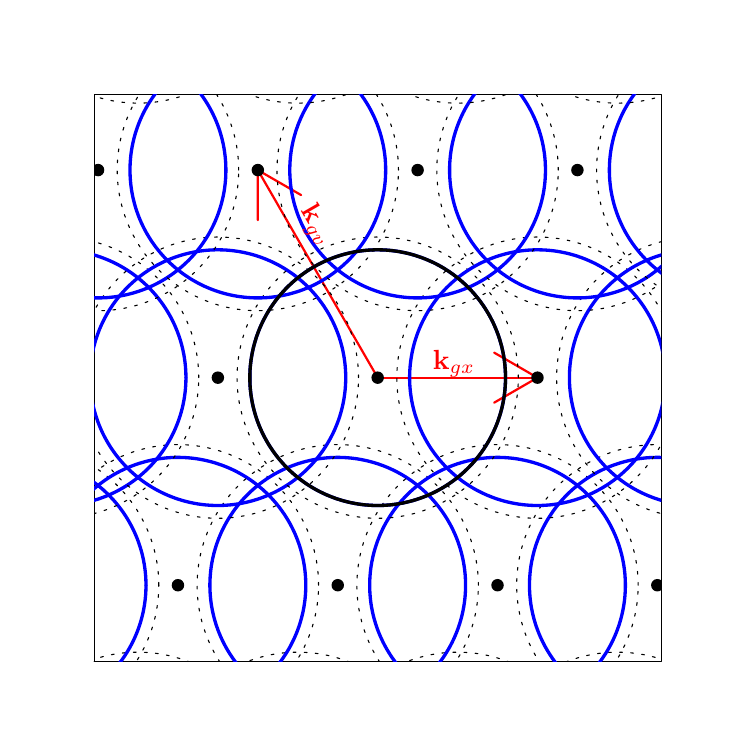
\begin{tikzpicture}[x=1pt,y=1pt]
\definecolor[named]{fillColor}{rgb}{1.00,1.00,1.00}
\path[use as bounding box,fill=fillColor,fill opacity=0.00] (0,0) rectangle (252.94,252.94);
\begin{scope}
\path[clip] (  0.00,  0.00) rectangle (252.94,252.94);
\definecolor[named]{drawColor}{rgb}{0.00,0.00,0.00}

\path[draw=drawColor,line width= 0.4pt,line join=round,line cap=round] ( 24.00, 24.00) --
	(228.94, 24.00) --
	(228.94,228.94) --
	( 24.00,228.94) --
	( 24.00, 24.00);
\end{scope}
\begin{scope}
\path[clip] ( 24.00, 24.00) rectangle (228.94,228.94);
\definecolor[named]{drawColor}{rgb}{0.00,0.00,0.00}

\path[draw=drawColor,line width= 0.4pt,line join=round,line cap=round] (126.47,126.47) --
	(126.47,126.47);
\definecolor[named]{drawColor}{rgb}{1.00,0.00,0.00}
\definecolor[named]{fillColor}{rgb}{1.00,1.00,1.00}

\path[draw=drawColor,line width= 0.8pt,line join=round,line cap=round,fill=fillColor] (126.47,126.47) -- (184.21,126.47);

\path[draw=drawColor,line width= 0.8pt,line join=round,line cap=round] (168.57,117.44) --
	(184.21,126.47) --
	(168.57,135.51);

\path[draw=drawColor,line width= 0.8pt,line join=round,line cap=round,fill=fillColor] (126.47,126.47) -- ( 83.17,201.48);

\path[draw=drawColor,line width= 0.8pt,line join=round,line cap=round] ( 98.81,192.45) --
	( 83.17,201.48) --
	( 83.17,183.41);
\definecolor[named]{drawColor}{rgb}{0.00,0.00,1.00}

\path[draw=drawColor,line width= 1.2pt,line join=round,line cap=round] ( 21.86,  0.00) --
	( 21.68,  0.31) --
	( 21.26,  1.00) --
	( 20.82,  1.68) --
	( 20.38,  2.35) --
	( 19.92,  3.02) --
	( 19.45,  3.68) --
	( 18.96,  4.32) --
	( 18.47,  4.97) --
	( 17.97,  5.60) --
	( 17.45,  6.22) --
	( 16.92,  6.83) --
	( 16.39,  7.44) --
	( 15.84,  8.03) --
	( 15.28,  8.62) --
	( 14.71,  9.19) --
	( 14.14,  9.76) --
	( 13.55, 10.31) --
	( 12.95, 10.86) --
	( 12.34, 11.39) --
	( 11.73, 11.92) --
	( 11.10, 12.43) --
	( 10.47, 12.93) --
	(  9.83, 13.42) --
	(  9.18, 13.90) --
	(  8.52, 14.37) --
	(  7.85, 14.83) --
	(  7.17, 15.27) --
	(  6.49, 15.70) --
	(  5.80, 16.12) --
	(  5.10, 16.53) --
	(  4.40, 16.93) --
	(  3.68, 17.31) --
	(  2.97, 17.68) --
	(  2.24, 18.04) --
	(  1.51, 18.39) --
	(  0.77, 18.72) --
	(  0.03, 19.04) --
	(  0.00, 19.05);
\definecolor[named]{drawColor}{rgb}{0.00,0.00,0.00}

\path[draw=drawColor,line width= 0.4pt,dash pattern=on 1pt off 3pt ,line join=round,line cap=round] ( 27.15,  0.00) --
	( 26.95,  0.37) --
	( 26.53,  1.16) --
	( 26.09,  1.93) --
	( 25.64,  2.69) --
	( 25.17,  3.45) --
	( 24.69,  4.20) --
	( 24.20,  4.94) --
	( 23.70,  5.67) --
	( 23.18,  6.40) --
	( 22.65,  7.11) --
	( 22.10,  7.82) --
	( 21.55,  8.51) --
	( 20.98,  9.20) --
	( 20.40,  9.87) --
	( 19.81, 10.54) --
	( 19.21, 11.19) --
	( 18.60, 11.83) --
	( 17.97, 12.47) --
	( 17.34, 13.09) --
	( 16.69, 13.70) --
	( 16.03, 14.30) --
	( 15.37, 14.89) --
	( 14.69, 15.46) --
	( 14.00, 16.03) --
	( 13.30, 16.58) --
	( 12.60, 17.12) --
	( 11.88, 17.65) --
	( 11.16, 18.16) --
	( 10.42, 18.66) --
	(  9.68, 19.15) --
	(  8.93, 19.63) --
	(  8.17, 20.09) --
	(  7.40, 20.54) --
	(  6.62, 20.97) --
	(  5.84, 21.40) --
	(  5.05, 21.80) --
	(  4.25, 22.20) --
	(  3.45, 22.58) --
	(  2.64, 22.94) --
	(  1.82, 23.30) --
	(  1.00, 23.63) --
	(  0.17, 23.96) --
	(  0.00, 24.02);
\definecolor[named]{drawColor}{rgb}{0.00,0.00,1.00}

\path[draw=drawColor,line width= 1.2pt,line join=round,line cap=round] ( 79.61,  0.00) --
	( 79.42,  0.31) --
	( 79.00,  1.00) --
	( 78.56,  1.68) --
	( 78.12,  2.35) --
	( 77.66,  3.02) --
	( 77.19,  3.68) --
	( 76.70,  4.32) --
	( 76.21,  4.97) --
	( 75.71,  5.60) --
	( 75.19,  6.22) --
	( 74.66,  6.83) --
	( 74.13,  7.44) --
	( 73.58,  8.03) --
	( 73.02,  8.62) --
	( 72.45,  9.19) --
	( 71.88,  9.76) --
	( 71.29, 10.31) --
	( 70.69, 10.86) --
	( 70.08, 11.39) --
	( 69.47, 11.92) --
	( 68.84, 12.43) --
	( 68.21, 12.93) --
	( 67.57, 13.42) --
	( 66.92, 13.90) --
	( 66.26, 14.37) --
	( 65.59, 14.83) --
	( 64.91, 15.27) --
	( 64.23, 15.70) --
	( 63.54, 16.12) --
	( 62.84, 16.53) --
	( 62.14, 16.93) --
	( 61.43, 17.31) --
	( 60.71, 17.68) --
	( 59.98, 18.04) --
	( 59.25, 18.39) --
	( 58.51, 18.72) --
	( 57.77, 19.04) --
	( 57.02, 19.35) --
	( 56.27, 19.64) --
	( 55.51, 19.92) --
	( 54.75, 20.19) --
	( 53.98, 20.44) --
	( 53.21, 20.68) --
	( 52.43, 20.91) --
	( 51.65, 21.12) --
	( 50.87, 21.32) --
	( 50.08, 21.51) --
	( 49.29, 21.68) --
	( 48.50, 21.84) --
	( 47.71, 21.98) --
	( 46.91, 22.11) --
	( 46.11, 22.23) --
	( 45.31, 22.33) --
	( 44.50, 22.42) --
	( 43.70, 22.49) --
	( 42.89, 22.55) --
	( 42.08, 22.60) --
	( 41.28, 22.63) --
	( 40.47, 22.65) --
	( 39.66, 22.65) --
	( 38.85, 22.64) --
	( 38.04, 22.62) --
	( 37.24, 22.58) --
	( 36.43, 22.52) --
	( 35.62, 22.46) --
	( 34.82, 22.38) --
	( 34.02, 22.28) --
	( 33.21, 22.17) --
	( 32.42, 22.05) --
	( 31.62, 21.91) --
	( 30.82, 21.76) --
	( 30.03, 21.59) --
	( 29.24, 21.42) --
	( 28.46, 21.22) --
	( 27.68, 21.02) --
	( 26.90, 20.80) --
	( 26.13, 20.56) --
	( 25.36, 20.32) --
	( 24.59, 20.06) --
	( 23.83, 19.78) --
	( 23.07, 19.49) --
	( 22.32, 19.19) --
	( 21.58, 18.88) --
	( 20.84, 18.55) --
	( 20.10, 18.21) --
	( 19.38, 17.86) --
	( 18.66, 17.50) --
	( 17.94, 17.12) --
	( 17.23, 16.73) --
	( 16.53, 16.33) --
	( 15.84, 15.91) --
	( 15.15, 15.49) --
	( 14.47, 15.05) --
	( 13.80, 14.60) --
	( 13.14, 14.14) --
	( 12.48, 13.66) --
	( 11.83, 13.18) --
	( 11.19, 12.68) --
	( 10.57, 12.17) --
	(  9.94, 11.66) --
	(  9.33, 11.13) --
	(  8.73, 10.59) --
	(  8.14, 10.04) --
	(  7.56,  9.48) --
	(  6.98,  8.91) --
	(  6.42,  8.33) --
	(  5.87,  7.74) --
	(  5.33,  7.14) --
	(  4.79,  6.53) --
	(  4.27,  5.91) --
	(  3.76,  5.28) --
	(  3.26,  4.65) --
	(  2.78,  4.00) --
	(  2.30,  3.35) --
	(  1.83,  2.69) --
	(  1.38,  2.02) --
	(  0.94,  1.34) --
	(  0.51,  0.65) --
	(  0.12,  0.00);
\definecolor[named]{drawColor}{rgb}{0.00,0.00,0.00}

\path[draw=drawColor,line width= 0.4pt,dash pattern=on 1pt off 3pt ,line join=round,line cap=round] ( 84.89,  0.00) --
	( 84.70,  0.37) --
	( 84.27,  1.16) --
	( 83.83,  1.93) --
	( 83.38,  2.69) --
	( 82.91,  3.45) --
	( 82.43,  4.20) --
	( 81.94,  4.94) --
	( 81.44,  5.67) --
	( 80.92,  6.40) --
	( 80.39,  7.11) --
	( 79.85,  7.82) --
	( 79.29,  8.51) --
	( 78.72,  9.20) --
	( 78.14,  9.87) --
	( 77.55, 10.54) --
	( 76.95, 11.19) --
	( 76.34, 11.83) --
	( 75.71, 12.47) --
	( 75.08, 13.09) --
	( 74.43, 13.70) --
	( 73.77, 14.30) --
	( 73.11, 14.89) --
	( 72.43, 15.46) --
	( 71.74, 16.03) --
	( 71.04, 16.58) --
	( 70.34, 17.12) --
	( 69.62, 17.65) --
	( 68.90, 18.16) --
	( 68.16, 18.66) --
	( 67.42, 19.15) --
	( 66.67, 19.63) --
	( 65.91, 20.09) --
	( 65.14, 20.54) --
	( 64.36, 20.97) --
	( 63.58, 21.40) --
	( 62.79, 21.80) --
	( 61.99, 22.20) --
	( 61.19, 22.58) --
	( 60.38, 22.94) --
	( 59.56, 23.30) --
	( 58.74, 23.63) --
	( 57.91, 23.96) --
	( 57.08, 24.27) --
	( 56.24, 24.56) --
	( 55.39, 24.84) --
	( 54.55, 25.10) --
	( 53.69, 25.35) --
	( 52.83, 25.59) --
	( 51.97, 25.81) --
	( 51.11, 26.01) --
	( 50.24, 26.20) --
	( 49.37, 26.38) --
	( 48.49, 26.53) --
	( 47.61, 26.68) --
	( 46.73, 26.81) --
	( 45.85, 26.92) --
	( 44.97, 27.01) --
	( 44.08, 27.10) --
	( 43.19, 27.16) --
	( 42.31, 27.21) --
	( 41.42, 27.25) --
	( 40.53, 27.27) --
	( 39.64, 27.27) --
	( 38.75, 27.26) --
	( 37.86, 27.23) --
	( 36.97, 27.19) --
	( 36.09, 27.13) --
	( 35.20, 27.06) --
	( 34.31, 26.97) --
	( 33.43, 26.86) --
	( 32.55, 26.74) --
	( 31.67, 26.61) --
	( 30.79, 26.46) --
	( 29.92, 26.29) --
	( 29.05, 26.11) --
	( 28.18, 25.91) --
	( 27.32, 25.70) --
	( 26.46, 25.47) --
	( 25.60, 25.23) --
	( 24.75, 24.97) --
	( 23.91, 24.70) --
	( 23.06, 24.42) --
	( 22.23, 24.11) --
	( 21.40, 23.80) --
	( 20.57, 23.47) --
	( 19.75, 23.12) --
	( 18.94, 22.76) --
	( 18.13, 22.39) --
	( 17.33, 22.00) --
	( 16.53, 21.60) --
	( 15.75, 21.19) --
	( 14.97, 20.76) --
	( 14.20, 20.32) --
	( 13.43, 19.86) --
	( 12.68, 19.39) --
	( 11.93, 18.91) --
	( 11.19, 18.41) --
	( 10.46, 17.90) --
	(  9.74, 17.38) --
	(  9.03, 16.85) --
	(  8.33, 16.30) --
	(  7.64, 15.75) --
	(  6.95, 15.18) --
	(  6.28, 14.59) --
	(  5.62, 14.00) --
	(  4.97, 13.40) --
	(  4.33, 12.78) --
	(  3.70, 12.15) --
	(  3.08, 11.51) --
	(  2.47, 10.86) --
	(  1.87, 10.20) --
	(  1.29,  9.53) --
	(  0.71,  8.85) --
	(  0.15,  8.16) --
	(  0.00,  7.97);
\definecolor[named]{drawColor}{rgb}{0.00,0.00,1.00}

\path[draw=drawColor,line width= 1.2pt,line join=round,line cap=round] ( 42.75, 51.47) --
	( 42.74, 52.27) --
	( 42.72, 53.08) --
	( 42.69, 53.89) --
	( 42.64, 54.70) --
	( 42.57, 55.50) --
	( 42.50, 56.31) --
	( 42.40, 57.11) --
	( 42.30, 57.91) --
	( 42.18, 58.71) --
	( 42.04, 59.51) --
	( 41.90, 60.30) --
	( 41.74, 61.10) --
	( 41.56, 61.89) --
	( 41.37, 62.67) --
	( 41.17, 63.45) --
	( 40.95, 64.23) --
	( 40.72, 65.01) --
	( 40.48, 65.78) --
	( 40.22, 66.54) --
	( 39.95, 67.31) --
	( 39.67, 68.06) --
	( 39.37, 68.82) --
	( 39.06, 69.56) --
	( 38.73, 70.30) --
	( 38.40, 71.04) --
	( 38.05, 71.77) --
	( 37.69, 72.49) --
	( 37.31, 73.21) --
	( 36.93, 73.92) --
	( 36.53, 74.62) --
	( 36.12, 75.32) --
	( 35.69, 76.01) --
	( 35.26, 76.69) --
	( 34.81, 77.36) --
	( 34.35, 78.03) --
	( 33.88, 78.68) --
	( 33.40, 79.33) --
	( 32.91, 79.97) --
	( 32.40, 80.60) --
	( 31.89, 81.23) --
	( 31.36, 81.84) --
	( 30.82, 82.45) --
	( 30.27, 83.04) --
	( 29.72, 83.63) --
	( 29.15, 84.20) --
	( 28.57, 84.77) --
	( 27.98, 85.32) --
	( 27.39, 85.87) --
	( 26.78, 86.40) --
	( 26.16, 86.92) --
	( 25.54, 87.44) --
	( 24.90, 87.94) --
	( 24.26, 88.43) --
	( 23.61, 88.91) --
	( 22.95, 89.38) --
	( 22.28, 89.83) --
	( 21.61, 90.28) --
	( 20.92, 90.71) --
	( 20.23, 91.13) --
	( 19.54, 91.54) --
	( 18.83, 91.93) --
	( 18.12, 92.32) --
	( 17.40, 92.69) --
	( 16.68, 93.05) --
	( 15.95, 93.39) --
	( 15.21, 93.73) --
	( 14.47, 94.05) --
	( 13.72, 94.35) --
	( 12.97, 94.65) --
	( 12.21, 94.93) --
	( 11.44, 95.19) --
	( 10.68, 95.45) --
	(  9.90, 95.69) --
	(  9.13, 95.92) --
	(  8.35, 96.13) --
	(  7.57, 96.33) --
	(  6.78, 96.51) --
	(  5.99, 96.69) --
	(  5.20, 96.84) --
	(  4.40, 96.99) --
	(  3.60, 97.12) --
	(  2.80, 97.24) --
	(  2.00, 97.34) --
	(  1.20, 97.43) --
	(  0.39, 97.50) --
	(  0.00, 97.53);

\path[draw=drawColor,line width= 1.2pt,line join=round,line cap=round] (  0.00,  5.40) --
	(  0.39,  5.43) --
	(  1.20,  5.50) --
	(  2.00,  5.59) --
	(  2.80,  5.69) --
	(  3.60,  5.81) --
	(  4.40,  5.94) --
	(  5.20,  6.09) --
	(  5.99,  6.24) --
	(  6.78,  6.42) --
	(  7.57,  6.60) --
	(  8.35,  6.80) --
	(  9.13,  7.01) --
	(  9.90,  7.24) --
	( 10.68,  7.48) --
	( 11.44,  7.74) --
	( 12.21,  8.00) --
	( 12.97,  8.28) --
	( 13.72,  8.58) --
	( 14.47,  8.88) --
	( 15.21,  9.20) --
	( 15.95,  9.54) --
	( 16.68,  9.88) --
	( 17.40, 10.24) --
	( 18.12, 10.61) --
	( 18.83, 11.00) --
	( 19.54, 11.39) --
	( 20.23, 11.80) --
	( 20.92, 12.22) --
	( 21.61, 12.65) --
	( 22.28, 13.10) --
	( 22.95, 13.55) --
	( 23.61, 14.02) --
	( 24.26, 14.50) --
	( 24.90, 14.99) --
	( 25.54, 15.49) --
	( 26.16, 16.01) --
	( 26.78, 16.53) --
	( 27.39, 17.06) --
	( 27.98, 17.61) --
	( 28.57, 18.16) --
	( 29.15, 18.73) --
	( 29.72, 19.30) --
	( 30.27, 19.89) --
	( 30.82, 20.48) --
	( 31.36, 21.09) --
	( 31.89, 21.70) --
	( 32.40, 22.33) --
	( 32.91, 22.96) --
	( 33.40, 23.60) --
	( 33.88, 24.25) --
	( 34.35, 24.90) --
	( 34.81, 25.57) --
	( 35.26, 26.24) --
	( 35.69, 26.92) --
	( 36.12, 27.61) --
	( 36.53, 28.31) --
	( 36.93, 29.01) --
	( 37.31, 29.72) --
	( 37.69, 30.44) --
	( 38.05, 31.16) --
	( 38.40, 31.89) --
	( 38.73, 32.63) --
	( 39.06, 33.37) --
	( 39.37, 34.11) --
	( 39.67, 34.87) --
	( 39.95, 35.62) --
	( 40.22, 36.39) --
	( 40.48, 37.15) --
	( 40.72, 37.92) --
	( 40.95, 38.70) --
	( 41.17, 39.48) --
	( 41.37, 40.26) --
	( 41.56, 41.04) --
	( 41.74, 41.83) --
	( 41.90, 42.63) --
	( 42.04, 43.42) --
	( 42.18, 44.22) --
	( 42.30, 45.02) --
	( 42.40, 45.82) --
	( 42.50, 46.62) --
	( 42.57, 47.43) --
	( 42.64, 48.23) --
	( 42.69, 49.04) --
	( 42.72, 49.85) --
	( 42.74, 50.66) --
	( 42.75, 51.47);
\definecolor[named]{drawColor}{rgb}{0.00,0.00,0.00}

\path[draw=drawColor,line width= 0.4pt,dash pattern=on 1pt off 3pt ,line join=round,line cap=round] ( 47.37, 51.47) --
	( 47.36, 52.35) --
	( 47.34, 53.24) --
	( 47.30, 54.13) --
	( 47.25, 55.02) --
	( 47.18, 55.91) --
	( 47.09, 56.79) --
	( 46.99, 57.67) --
	( 46.87, 58.56) --
	( 46.74, 59.44) --
	( 46.59, 60.31) --
	( 46.43, 61.19) --
	( 46.25, 62.06) --
	( 46.06, 62.93) --
	( 45.85, 63.79) --
	( 45.63, 64.65) --
	( 45.39, 65.51) --
	( 45.14, 66.36) --
	( 44.87, 67.21) --
	( 44.59, 68.05) --
	( 44.29, 68.89) --
	( 43.98, 69.72) --
	( 43.65, 70.55) --
	( 43.31, 71.37) --
	( 42.95, 72.19) --
	( 42.58, 73.00) --
	( 42.20, 73.80) --
	( 41.80, 74.59) --
	( 41.39, 75.38) --
	( 40.96, 76.16) --
	( 40.53, 76.94) --
	( 40.07, 77.70) --
	( 39.61, 78.46) --
	( 39.13, 79.21) --
	( 38.64, 79.95) --
	( 38.13, 80.68) --
	( 37.61, 81.40) --
	( 37.08, 82.12) --
	( 36.54, 82.82) --
	( 35.99, 83.52) --
	( 35.42, 84.20) --
	( 34.84, 84.88) --
	( 34.25, 85.54) --
	( 33.65, 86.20) --
	( 33.03, 86.84) --
	( 32.41, 87.47) --
	( 31.77, 88.10) --
	( 31.13, 88.71) --
	( 30.47, 89.31) --
	( 29.80, 89.89) --
	( 29.12, 90.47) --
	( 28.44, 91.03) --
	( 27.74, 91.59) --
	( 27.03, 92.13) --
	( 26.32, 92.65) --
	( 25.59, 93.17) --
	( 24.86, 93.67) --
	( 24.11, 94.16) --
	( 23.36, 94.63) --
	( 22.60, 95.10) --
	( 21.83, 95.55) --
	( 21.06, 95.98) --
	( 20.28, 96.40) --
	( 19.49, 96.81) --
	( 18.69, 97.21) --
	( 17.89, 97.59) --
	( 17.07, 97.95) --
	( 16.26, 98.30) --
	( 15.44, 98.64) --
	( 14.61, 98.97) --
	( 13.77, 99.27) --
	( 12.93, 99.57) --
	( 12.09, 99.85) --
	( 11.24,100.11) --
	( 10.39,100.36) --
	(  9.53,100.60) --
	(  8.67,100.82) --
	(  7.80,101.02) --
	(  6.93,101.21) --
	(  6.06,101.38) --
	(  5.18,101.54) --
	(  4.31,101.68) --
	(  3.43,101.81) --
	(  2.54,101.93) --
	(  1.66,102.02) --
	(  0.78,102.10) --
	(  0.00,102.16);

\path[draw=drawColor,line width= 0.4pt,dash pattern=on 1pt off 3pt ,line join=round,line cap=round] (  0.00,  0.77) --
	(  0.78,  0.83) --
	(  1.66,  0.91) --
	(  2.54,  1.00) --
	(  3.43,  1.12) --
	(  4.31,  1.25) --
	(  5.18,  1.39) --
	(  6.06,  1.55) --
	(  6.93,  1.72) --
	(  7.80,  1.91) --
	(  8.67,  2.11) --
	(  9.53,  2.33) --
	( 10.39,  2.57) --
	( 11.24,  2.82) --
	( 12.09,  3.08) --
	( 12.93,  3.36) --
	( 13.77,  3.66) --
	( 14.61,  3.96) --
	( 15.44,  4.29) --
	( 16.26,  4.63) --
	( 17.07,  4.98) --
	( 17.89,  5.34) --
	( 18.69,  5.72) --
	( 19.49,  6.12) --
	( 20.28,  6.53) --
	( 21.06,  6.95) --
	( 21.83,  7.38) --
	( 22.60,  7.83) --
	( 23.36,  8.30) --
	( 24.11,  8.77) --
	( 24.86,  9.26) --
	( 25.59,  9.76) --
	( 26.32, 10.28) --
	( 27.03, 10.80) --
	( 27.74, 11.34) --
	( 28.44, 11.90) --
	( 29.12, 12.46) --
	( 29.80, 13.04) --
	( 30.47, 13.62) --
	( 31.13, 14.22) --
	( 31.77, 14.83) --
	( 32.41, 15.46) --
	( 33.03, 16.09) --
	( 33.65, 16.73) --
	( 34.25, 17.39) --
	( 34.84, 18.05) --
	( 35.42, 18.73) --
	( 35.99, 19.41) --
	( 36.54, 20.11) --
	( 37.08, 20.81) --
	( 37.61, 21.53) --
	( 38.13, 22.25) --
	( 38.64, 22.98) --
	( 39.13, 23.72) --
	( 39.61, 24.47) --
	( 40.07, 25.23) --
	( 40.53, 25.99) --
	( 40.96, 26.77) --
	( 41.39, 27.55) --
	( 41.80, 28.34) --
	( 42.20, 29.13) --
	( 42.58, 29.93) --
	( 42.95, 30.74) --
	( 43.31, 31.56) --
	( 43.65, 32.38) --
	( 43.98, 33.21) --
	( 44.29, 34.04) --
	( 44.59, 34.88) --
	( 44.87, 35.72) --
	( 45.14, 36.57) --
	( 45.39, 37.42) --
	( 45.63, 38.28) --
	( 45.85, 39.14) --
	( 46.06, 40.00) --
	( 46.25, 40.87) --
	( 46.43, 41.74) --
	( 46.59, 42.62) --
	( 46.74, 43.49) --
	( 46.87, 44.37) --
	( 46.99, 45.26) --
	( 47.09, 46.14) --
	( 47.18, 47.02) --
	( 47.25, 47.91) --
	( 47.30, 48.80) --
	( 47.34, 49.69) --
	( 47.36, 50.58) --
	( 47.37, 51.47);

\path[draw=drawColor,line width= 0.4pt,dash pattern=on 1pt off 3pt ,line join=round,line cap=round] (  4.06,126.47) --
	(  4.06,127.36) --
	(  4.03,128.25) --
	(  3.99,129.14) --
	(  3.94,130.03) --
	(  3.87,130.91) --
	(  3.78,131.80) --
	(  3.68,132.68) --
	(  3.57,133.56) --
	(  3.44,134.44) --
	(  3.29,135.32) --
	(  3.13,136.20) --
	(  2.95,137.07) --
	(  2.75,137.93) --
	(  2.55,138.80) --
	(  2.32,139.66) --
	(  2.09,140.52) --
	(  1.83,141.37) --
	(  1.56,142.22) --
	(  1.28,143.06) --
	(  0.98,143.90) --
	(  0.67,144.73) --
	(  0.34,145.56) --
	(  0.00,146.38) --
	(  0.00,146.39);

\path[draw=drawColor,line width= 0.4pt,dash pattern=on 1pt off 3pt ,line join=round,line cap=round] (  0.00,106.56) --
	(  0.00,106.57) --
	(  0.34,107.39) --
	(  0.67,108.21) --
	(  0.98,109.05) --
	(  1.28,109.88) --
	(  1.56,110.73) --
	(  1.83,111.58) --
	(  2.09,112.43) --
	(  2.32,113.28) --
	(  2.55,114.15) --
	(  2.75,115.01) --
	(  2.95,115.88) --
	(  3.13,116.75) --
	(  3.29,117.62) --
	(  3.44,118.50) --
	(  3.57,119.38) --
	(  3.68,120.26) --
	(  3.78,121.15) --
	(  3.87,122.03) --
	(  3.94,122.92) --
	(  3.99,123.81) --
	(  4.03,124.69) --
	(  4.06,125.58) --
	(  4.06,126.47);
\definecolor[named]{drawColor}{rgb}{0.00,0.00,1.00}

\path[draw=drawColor,line width= 1.2pt,line join=round,line cap=round] (137.35,  0.00) --
	(137.16,  0.31) --
	(136.74,  1.00) --
	(136.30,  1.68) --
	(135.86,  2.35) --
	(135.40,  3.02) --
	(134.93,  3.68) --
	(134.44,  4.32) --
	(133.95,  4.97) --
	(133.45,  5.60) --
	(132.93,  6.22) --
	(132.41,  6.83) --
	(131.87,  7.44) --
	(131.32,  8.03) --
	(130.76,  8.62) --
	(130.20,  9.19) --
	(129.62,  9.76) --
	(129.03, 10.31) --
	(128.43, 10.86) --
	(127.83, 11.39) --
	(127.21, 11.92) --
	(126.58, 12.43) --
	(125.95, 12.93) --
	(125.31, 13.42) --
	(124.66, 13.90) --
	(124.00, 14.37) --
	(123.33, 14.83) --
	(122.65, 15.27) --
	(121.97, 15.70) --
	(121.28, 16.12) --
	(120.58, 16.53) --
	(119.88, 16.93) --
	(119.17, 17.31) --
	(118.45, 17.68) --
	(117.72, 18.04) --
	(116.99, 18.39) --
	(116.26, 18.72) --
	(115.51, 19.04) --
	(114.77, 19.35) --
	(114.01, 19.64) --
	(113.25, 19.92) --
	(112.49, 20.19) --
	(111.72, 20.44) --
	(110.95, 20.68) --
	(110.18, 20.91) --
	(109.40, 21.12) --
	(108.61, 21.32) --
	(107.83, 21.51) --
	(107.04, 21.68) --
	(106.24, 21.84) --
	(105.45, 21.98) --
	(104.65, 22.11) --
	(103.85, 22.23) --
	(103.05, 22.33) --
	(102.24, 22.42) --
	(101.44, 22.49) --
	(100.63, 22.55) --
	( 99.82, 22.60) --
	( 99.02, 22.63) --
	( 98.21, 22.65) --
	( 97.40, 22.65) --
	( 96.59, 22.64) --
	( 95.78, 22.62) --
	( 94.98, 22.58) --
	( 94.17, 22.52) --
	( 93.36, 22.46) --
	( 92.56, 22.38) --
	( 91.76, 22.28) --
	( 90.96, 22.17) --
	( 90.16, 22.05) --
	( 89.36, 21.91) --
	( 88.57, 21.76) --
	( 87.77, 21.59) --
	( 86.99, 21.42) --
	( 86.20, 21.22) --
	( 85.42, 21.02) --
	( 84.64, 20.80) --
	( 83.87, 20.56) --
	( 83.10, 20.32) --
	( 82.33, 20.06) --
	( 81.57, 19.78) --
	( 80.81, 19.49) --
	( 80.06, 19.19) --
	( 79.32, 18.88) --
	( 78.58, 18.55) --
	( 77.85, 18.21) --
	( 77.12, 17.86) --
	( 76.40, 17.50) --
	( 75.68, 17.12) --
	( 74.97, 16.73) --
	( 74.27, 16.33) --
	( 73.58, 15.91) --
	( 72.89, 15.49) --
	( 72.21, 15.05) --
	( 71.54, 14.60) --
	( 70.88, 14.14) --
	( 70.22, 13.66) --
	( 69.57, 13.18) --
	( 68.94, 12.68) --
	( 68.31, 12.17) --
	( 67.69, 11.66) --
	( 67.07, 11.13) --
	( 66.47, 10.59) --
	( 65.88, 10.04) --
	( 65.30,  9.48) --
	( 64.72,  8.91) --
	( 64.16,  8.33) --
	( 63.61,  7.74) --
	( 63.07,  7.14) --
	( 62.53,  6.53) --
	( 62.01,  5.91) --
	( 61.50,  5.28) --
	( 61.00,  4.65) --
	( 60.52,  4.00) --
	( 60.04,  3.35) --
	( 59.58,  2.69) --
	( 59.12,  2.02) --
	( 58.68,  1.34) --
	( 58.25,  0.65) --
	( 57.86,  0.00);
\definecolor[named]{drawColor}{rgb}{0.00,0.00,0.00}

\path[draw=drawColor,line width= 0.4pt,dash pattern=on 1pt off 3pt ,line join=round,line cap=round] (142.63,  0.00) --
	(142.44,  0.37) --
	(142.01,  1.16) --
	(141.57,  1.93) --
	(141.12,  2.69) --
	(140.65,  3.45) --
	(140.17,  4.20) --
	(139.68,  4.94) --
	(139.18,  5.67) --
	(138.66,  6.40) --
	(138.13,  7.11) --
	(137.59,  7.82) --
	(137.03,  8.51) --
	(136.46,  9.20) --
	(135.89,  9.87) --
	(135.30, 10.54) --
	(134.69, 11.19) --
	(134.08, 11.83) --
	(133.45, 12.47) --
	(132.82, 13.09) --
	(132.17, 13.70) --
	(131.52, 14.30) --
	(130.85, 14.89) --
	(130.17, 15.46) --
	(129.48, 16.03) --
	(128.79, 16.58) --
	(128.08, 17.12) --
	(127.36, 17.65) --
	(126.64, 18.16) --
	(125.90, 18.66) --
	(125.16, 19.15) --
	(124.41, 19.63) --
	(123.65, 20.09) --
	(122.88, 20.54) --
	(122.11, 20.97) --
	(121.32, 21.40) --
	(120.53, 21.80) --
	(119.74, 22.20) --
	(118.93, 22.58) --
	(118.12, 22.94) --
	(117.30, 23.30) --
	(116.48, 23.63) --
	(115.65, 23.96) --
	(114.82, 24.27) --
	(113.98, 24.56) --
	(113.14, 24.84) --
	(112.29, 25.10) --
	(111.43, 25.35) --
	(110.57, 25.59) --
	(109.71, 25.81) --
	(108.85, 26.01) --
	(107.98, 26.20) --
	(107.11, 26.38) --
	(106.23, 26.53) --
	(105.35, 26.68) --
	(104.47, 26.81) --
	(103.59, 26.92) --
	(102.71, 27.01) --
	(101.82, 27.10) --
	(100.93, 27.16) --
	(100.05, 27.21) --
	( 99.16, 27.25) --
	( 98.27, 27.27) --
	( 97.38, 27.27) --
	( 96.49, 27.26) --
	( 95.60, 27.23) --
	( 94.71, 27.19) --
	( 93.83, 27.13) --
	( 92.94, 27.06) --
	( 92.05, 26.97) --
	( 91.17, 26.86) --
	( 90.29, 26.74) --
	( 89.41, 26.61) --
	( 88.54, 26.46) --
	( 87.66, 26.29) --
	( 86.79, 26.11) --
	( 85.92, 25.91) --
	( 85.06, 25.70) --
	( 84.20, 25.47) --
	( 83.34, 25.23) --
	( 82.49, 24.97) --
	( 81.65, 24.70) --
	( 80.80, 24.42) --
	( 79.97, 24.11) --
	( 79.14, 23.80) --
	( 78.31, 23.47) --
	( 77.49, 23.12) --
	( 76.68, 22.76) --
	( 75.87, 22.39) --
	( 75.07, 22.00) --
	( 74.28, 21.60) --
	( 73.49, 21.19) --
	( 72.71, 20.76) --
	( 71.94, 20.32) --
	( 71.17, 19.86) --
	( 70.42, 19.39) --
	( 69.67, 18.91) --
	( 68.93, 18.41) --
	( 68.20, 17.90) --
	( 67.48, 17.38) --
	( 66.77, 16.85) --
	( 66.07, 16.30) --
	( 65.38, 15.75) --
	( 64.69, 15.18) --
	( 64.02, 14.59) --
	( 63.36, 14.00) --
	( 62.71, 13.40) --
	( 62.07, 12.78) --
	( 61.44, 12.15) --
	( 60.82, 11.51) --
	( 60.21, 10.86) --
	( 59.61, 10.20) --
	( 59.03,  9.53) --
	( 58.45,  8.85) --
	( 57.89,  8.16) --
	( 57.34,  7.46) --
	( 56.81,  6.76) --
	( 56.28,  6.04) --
	( 55.77,  5.31) --
	( 55.27,  4.57) --
	( 54.79,  3.83) --
	( 54.32,  3.07) --
	( 53.86,  2.31) --
	( 53.41,  1.54) --
	( 52.98,  0.77) --
	( 52.57,  0.00);
\definecolor[named]{fillColor}{rgb}{0.00,0.00,0.00}

\path[fill=fillColor] ( 54.30, 51.47) circle (  2.25);
\definecolor[named]{drawColor}{rgb}{0.00,0.00,1.00}

\path[draw=drawColor,line width= 1.2pt,line join=round,line cap=round] (100.49, 51.47) --
	(100.48, 52.27) --
	(100.46, 53.08) --
	(100.43, 53.89) --
	(100.38, 54.70) --
	(100.31, 55.50) --
	(100.24, 56.31) --
	(100.15, 57.11) --
	(100.04, 57.91) --
	( 99.92, 58.71) --
	( 99.79, 59.51) --
	( 99.64, 60.30) --
	( 99.48, 61.10) --
	( 99.30, 61.89) --
	( 99.11, 62.67) --
	( 98.91, 63.45) --
	( 98.69, 64.23) --
	( 98.46, 65.01) --
	( 98.22, 65.78) --
	( 97.96, 66.54) --
	( 97.69, 67.31) --
	( 97.41, 68.06) --
	( 97.11, 68.82) --
	( 96.80, 69.56) --
	( 96.48, 70.30) --
	( 96.14, 71.04) --
	( 95.79, 71.77) --
	( 95.43, 72.49) --
	( 95.05, 73.21) --
	( 94.67, 73.92) --
	( 94.27, 74.62) --
	( 93.86, 75.32) --
	( 93.43, 76.01) --
	( 93.00, 76.69) --
	( 92.55, 77.36) --
	( 92.09, 78.03) --
	( 91.62, 78.68) --
	( 91.14, 79.33) --
	( 90.65, 79.97) --
	( 90.14, 80.60) --
	( 89.63, 81.23) --
	( 89.10, 81.84) --
	( 88.56, 82.45) --
	( 88.02, 83.04) --
	( 87.46, 83.63) --
	( 86.89, 84.20) --
	( 86.31, 84.77) --
	( 85.72, 85.32) --
	( 85.13, 85.87) --
	( 84.52, 86.40) --
	( 83.90, 86.92) --
	( 83.28, 87.44) --
	( 82.64, 87.94) --
	( 82.00, 88.43) --
	( 81.35, 88.91) --
	( 80.69, 89.38) --
	( 80.02, 89.83) --
	( 79.35, 90.28) --
	( 78.67, 90.71) --
	( 77.97, 91.13) --
	( 77.28, 91.54) --
	( 76.57, 91.93) --
	( 75.86, 92.32) --
	( 75.14, 92.69) --
	( 74.42, 93.05) --
	( 73.69, 93.39) --
	( 72.95, 93.73) --
	( 72.21, 94.05) --
	( 71.46, 94.35) --
	( 70.71, 94.65) --
	( 69.95, 94.93) --
	( 69.19, 95.19) --
	( 68.42, 95.45) --
	( 67.65, 95.69) --
	( 66.87, 95.92) --
	( 66.09, 96.13) --
	( 65.31, 96.33) --
	( 64.52, 96.51) --
	( 63.73, 96.69) --
	( 62.94, 96.84) --
	( 62.14, 96.99) --
	( 61.34, 97.12) --
	( 60.54, 97.24) --
	( 59.74, 97.34) --
	( 58.94, 97.43) --
	( 58.13, 97.50) --
	( 57.33, 97.56) --
	( 56.52, 97.61) --
	( 55.71, 97.64) --
	( 54.90, 97.66) --
	( 54.09, 97.66) --
	( 53.29, 97.65) --
	( 52.48, 97.62) --
	( 51.67, 97.59) --
	( 50.86, 97.53) --
	( 50.06, 97.47) --
	( 49.25, 97.38) --
	( 48.45, 97.29) --
	( 47.65, 97.18) --
	( 46.85, 97.06) --
	( 46.05, 96.92) --
	( 45.26, 96.77) --
	( 44.47, 96.60) --
	( 43.68, 96.42) --
	( 42.89, 96.23) --
	( 42.11, 96.02) --
	( 41.33, 95.80) --
	( 40.56, 95.57) --
	( 39.79, 95.32) --
	( 39.03, 95.06) --
	( 38.26, 94.79) --
	( 37.51, 94.50) --
	( 36.76, 94.20) --
	( 36.01, 93.89) --
	( 35.27, 93.56) --
	( 34.54, 93.22) --
	( 33.81, 92.87) --
	( 33.09, 92.51) --
	( 32.38, 92.13) --
	( 31.67, 91.74) --
	( 30.97, 91.34) --
	( 30.27, 90.92) --
	( 29.58, 90.49) --
	( 28.91, 90.06) --
	( 28.23, 89.61) --
	( 27.57, 89.14) --
	( 26.92, 88.67) --
	( 26.27, 88.19) --
	( 25.63, 87.69) --
	( 25.00, 87.18) --
	( 24.38, 86.66) --
	( 23.77, 86.14) --
	( 23.17, 85.60) --
	( 22.57, 85.05) --
	( 21.99, 84.49) --
	( 21.42, 83.91) --
	( 20.86, 83.33) --
	( 20.30, 82.74) --
	( 19.76, 82.14) --
	( 19.23, 81.54) --
	( 18.71, 80.92) --
	( 18.20, 80.29) --
	( 17.70, 79.65) --
	( 17.21, 79.01) --
	( 16.73, 78.36) --
	( 16.27, 77.69) --
	( 15.82, 77.02) --
	( 15.38, 76.35) --
	( 14.95, 75.66) --
	( 14.53, 74.97) --
	( 14.12, 74.27) --
	( 13.73, 73.56) --
	( 13.35, 72.85) --
	( 12.98, 72.13) --
	( 12.63, 71.40) --
	( 12.28, 70.67) --
	( 11.95, 69.93) --
	( 11.64, 69.19) --
	( 11.33, 68.44) --
	( 11.04, 67.69) --
	( 10.77, 66.93) --
	( 10.50, 66.16) --
	( 10.25, 65.39) --
	( 10.01, 64.62) --
	(  9.79, 63.84) --
	(  9.58, 63.06) --
	(  9.39, 62.28) --
	(  9.20, 61.49) --
	(  9.03, 60.70) --
	(  8.88, 59.91) --
	(  8.74, 59.11) --
	(  8.61, 58.31) --
	(  8.50, 57.51) --
	(  8.40, 56.71) --
	(  8.32, 55.90) --
	(  8.24, 55.10) --
	(  8.19, 54.29) --
	(  8.15, 53.49) --
	(  8.12, 52.68) --
	(  8.10, 51.87) --
	(  8.10, 51.06) --
	(  8.12, 50.25) --
	(  8.15, 49.44) --
	(  8.19, 48.64) --
	(  8.24, 47.83) --
	(  8.32, 47.03) --
	(  8.40, 46.22) --
	(  8.50, 45.42) --
	(  8.61, 44.62) --
	(  8.74, 43.82) --
	(  8.88, 43.02) --
	(  9.03, 42.23) --
	(  9.20, 41.44) --
	(  9.39, 40.65) --
	(  9.58, 39.87) --
	(  9.79, 39.09) --
	( 10.01, 38.31) --
	( 10.25, 37.54) --
	( 10.50, 36.77) --
	( 10.77, 36.00) --
	( 11.04, 35.24) --
	( 11.33, 34.49) --
	( 11.64, 33.74) --
	( 11.95, 33.00) --
	( 12.28, 32.26) --
	( 12.63, 31.53) --
	( 12.98, 30.80) --
	( 13.35, 30.08) --
	( 13.73, 29.37) --
	( 14.12, 28.66) --
	( 14.53, 27.96) --
	( 14.95, 27.27) --
	( 15.38, 26.58) --
	( 15.82, 25.91) --
	( 16.27, 25.24) --
	( 16.73, 24.57) --
	( 17.21, 23.92) --
	( 17.70, 23.28) --
	( 18.20, 22.64) --
	( 18.71, 22.01) --
	( 19.23, 21.39) --
	( 19.76, 20.79) --
	( 20.30, 20.19) --
	( 20.86, 19.60) --
	( 21.42, 19.02) --
	( 21.99, 18.44) --
	( 22.57, 17.88) --
	( 23.17, 17.33) --
	( 23.77, 16.79) --
	( 24.38, 16.27) --
	( 25.00, 15.75) --
	( 25.63, 15.24) --
	( 26.27, 14.74) --
	( 26.92, 14.26) --
	( 27.57, 13.79) --
	( 28.23, 13.32) --
	( 28.91, 12.87) --
	( 29.58, 12.44) --
	( 30.27, 12.01) --
	( 30.97, 11.59) --
	( 31.67, 11.19) --
	( 32.38, 10.80) --
	( 33.09, 10.42) --
	( 33.81, 10.06) --
	( 34.54,  9.71) --
	( 35.27,  9.37) --
	( 36.01,  9.04) --
	( 36.76,  8.73) --
	( 37.51,  8.43) --
	( 38.26,  8.14) --
	( 39.03,  7.87) --
	( 39.79,  7.61) --
	( 40.56,  7.36) --
	( 41.33,  7.13) --
	( 42.11,  6.91) --
	( 42.89,  6.70) --
	( 43.68,  6.51) --
	( 44.47,  6.33) --
	( 45.26,  6.16) --
	( 46.05,  6.01) --
	( 46.85,  5.87) --
	( 47.65,  5.75) --
	( 48.45,  5.64) --
	( 49.25,  5.55) --
	( 50.06,  5.46) --
	( 50.86,  5.40) --
	( 51.67,  5.34) --
	( 52.48,  5.31) --
	( 53.29,  5.28) --
	( 54.09,  5.27) --
	( 54.90,  5.27) --
	( 55.71,  5.29) --
	( 56.52,  5.32) --
	( 57.33,  5.37) --
	( 58.13,  5.43) --
	( 58.94,  5.50) --
	( 59.74,  5.59) --
	( 60.54,  5.69) --
	( 61.34,  5.81) --
	( 62.14,  5.94) --
	( 62.94,  6.09) --
	( 63.73,  6.24) --
	( 64.52,  6.42) --
	( 65.31,  6.60) --
	( 66.09,  6.80) --
	( 66.87,  7.01) --
	( 67.65,  7.24) --
	( 68.42,  7.48) --
	( 69.19,  7.74) --
	( 69.95,  8.00) --
	( 70.71,  8.28) --
	( 71.46,  8.58) --
	( 72.21,  8.88) --
	( 72.95,  9.20) --
	( 73.69,  9.54) --
	( 74.42,  9.88) --
	( 75.14, 10.24) --
	( 75.86, 10.61) --
	( 76.57, 11.00) --
	( 77.28, 11.39) --
	( 77.97, 11.80) --
	( 78.67, 12.22) --
	( 79.35, 12.65) --
	( 80.02, 13.10) --
	( 80.69, 13.55) --
	( 81.35, 14.02) --
	( 82.00, 14.50) --
	( 82.64, 14.99) --
	( 83.28, 15.49) --
	( 83.90, 16.01) --
	( 84.52, 16.53) --
	( 85.13, 17.06) --
	( 85.72, 17.61) --
	( 86.31, 18.16) --
	( 86.89, 18.73) --
	( 87.46, 19.30) --
	( 88.02, 19.89) --
	( 88.56, 20.48) --
	( 89.10, 21.09) --
	( 89.63, 21.70) --
	( 90.14, 22.33) --
	( 90.65, 22.96) --
	( 91.14, 23.60) --
	( 91.62, 24.25) --
	( 92.09, 24.90) --
	( 92.55, 25.57) --
	( 93.00, 26.24) --
	( 93.43, 26.92) --
	( 93.86, 27.61) --
	( 94.27, 28.31) --
	( 94.67, 29.01) --
	( 95.05, 29.72) --
	( 95.43, 30.44) --
	( 95.79, 31.16) --
	( 96.14, 31.89) --
	( 96.48, 32.63) --
	( 96.80, 33.37) --
	( 97.11, 34.11) --
	( 97.41, 34.87) --
	( 97.69, 35.62) --
	( 97.96, 36.39) --
	( 98.22, 37.15) --
	( 98.46, 37.92) --
	( 98.69, 38.70) --
	( 98.91, 39.48) --
	( 99.11, 40.26) --
	( 99.30, 41.04) --
	( 99.48, 41.83) --
	( 99.64, 42.63) --
	( 99.79, 43.42) --
	( 99.92, 44.22) --
	(100.04, 45.02) --
	(100.15, 45.82) --
	(100.24, 46.62) --
	(100.31, 47.43) --
	(100.38, 48.23) --
	(100.43, 49.04) --
	(100.46, 49.85) --
	(100.48, 50.66) --
	(100.49, 51.47);
\definecolor[named]{drawColor}{rgb}{0.00,0.00,0.00}

\path[draw=drawColor,line width= 0.4pt,dash pattern=on 1pt off 3pt ,line join=round,line cap=round] (105.11, 51.47) --
	(105.10, 52.35) --
	(105.08, 53.24) --
	(105.04, 54.13) --
	(104.99, 55.02) --
	(104.92, 55.91) --
	(104.83, 56.79) --
	(104.73, 57.67) --
	(104.61, 58.56) --
	(104.48, 59.44) --
	(104.33, 60.31) --
	(104.17, 61.19) --
	(103.99, 62.06) --
	(103.80, 62.93) --
	(103.59, 63.79) --
	(103.37, 64.65) --
	(103.13, 65.51) --
	(102.88, 66.36) --
	(102.61, 67.21) --
	(102.33, 68.05) --
	(102.03, 68.89) --
	(101.72, 69.72) --
	(101.39, 70.55) --
	(101.05, 71.37) --
	(100.69, 72.19) --
	(100.32, 73.00) --
	( 99.94, 73.80) --
	( 99.54, 74.59) --
	( 99.13, 75.38) --
	( 98.71, 76.16) --
	( 98.27, 76.94) --
	( 97.81, 77.70) --
	( 97.35, 78.46) --
	( 96.87, 79.21) --
	( 96.38, 79.95) --
	( 95.87, 80.68) --
	( 95.35, 81.40) --
	( 94.82, 82.12) --
	( 94.28, 82.82) --
	( 93.73, 83.52) --
	( 93.16, 84.20) --
	( 92.58, 84.88) --
	( 91.99, 85.54) --
	( 91.39, 86.20) --
	( 90.77, 86.84) --
	( 90.15, 87.47) --
	( 89.51, 88.10) --
	( 88.87, 88.71) --
	( 88.21, 89.31) --
	( 87.54, 89.89) --
	( 86.86, 90.47) --
	( 86.18, 91.03) --
	( 85.48, 91.59) --
	( 84.77, 92.13) --
	( 84.06, 92.65) --
	( 83.33, 93.17) --
	( 82.60, 93.67) --
	( 81.85, 94.16) --
	( 81.10, 94.63) --
	( 80.34, 95.10) --
	( 79.58, 95.55) --
	( 78.80, 95.98) --
	( 78.02, 96.40) --
	( 77.23, 96.81) --
	( 76.43, 97.21) --
	( 75.63, 97.59) --
	( 74.82, 97.95) --
	( 74.00, 98.30) --
	( 73.18, 98.64) --
	( 72.35, 98.97) --
	( 71.51, 99.27) --
	( 70.67, 99.57) --
	( 69.83, 99.85) --
	( 68.98,100.11) --
	( 68.13,100.36) --
	( 67.27,100.60) --
	( 66.41,100.82) --
	( 65.54,101.02) --
	( 64.67,101.21) --
	( 63.80,101.38) --
	( 62.93,101.54) --
	( 62.05,101.68) --
	( 61.17,101.81) --
	( 60.29,101.93) --
	( 59.40,102.02) --
	( 58.52,102.10) --
	( 57.63,102.17) --
	( 56.74,102.22) --
	( 55.85,102.26) --
	( 54.96,102.28) --
	( 54.07,102.28) --
	( 53.18,102.27) --
	( 52.30,102.24) --
	( 51.41,102.20) --
	( 50.52,102.14) --
	( 49.63,102.07) --
	( 48.75,101.98) --
	( 47.87,101.87) --
	( 46.98,101.75) --
	( 46.11,101.62) --
	( 45.23,101.46) --
	( 44.36,101.30) --
	( 43.49,101.12) --
	( 42.62,100.92) --
	( 41.75,100.71) --
	( 40.89,100.48) --
	( 40.04,100.24) --
	( 39.19, 99.98) --
	( 38.34, 99.71) --
	( 37.50, 99.42) --
	( 36.66, 99.12) --
	( 35.83, 98.81) --
	( 35.00, 98.47) --
	( 34.19, 98.13) --
	( 33.37, 97.77) --
	( 32.56, 97.40) --
	( 31.76, 97.01) --
	( 30.97, 96.61) --
	( 30.18, 96.19) --
	( 29.40, 95.77) --
	( 28.63, 95.32) --
	( 27.87, 94.87) --
	( 27.11, 94.40) --
	( 26.37, 93.92) --
	( 25.63, 93.42) --
	( 24.90, 92.91) --
	( 24.18, 92.39) --
	( 23.47, 91.86) --
	( 22.76, 91.31) --
	( 22.07, 90.75) --
	( 21.39, 90.18) --
	( 20.72, 89.60) --
	( 20.05, 89.01) --
	( 19.40, 88.40) --
	( 18.76, 87.79) --
	( 18.13, 87.16) --
	( 17.51, 86.52) --
	( 16.90, 85.87) --
	( 16.31, 85.21) --
	( 15.72, 84.54) --
	( 15.15, 83.86) --
	( 14.59, 83.17) --
	( 14.04, 82.47) --
	( 13.50, 81.76) --
	( 12.98, 81.04) --
	( 12.47, 80.32) --
	( 11.97, 79.58) --
	( 11.48, 78.84) --
	( 11.01, 78.08) --
	( 10.55, 77.32) --
	( 10.11, 76.55) --
	(  9.67, 75.77) --
	(  9.25, 74.99) --
	(  8.85, 74.20) --
	(  8.46, 73.40) --
	(  8.08, 72.59) --
	(  7.72, 71.78) --
	(  7.37, 70.96) --
	(  7.04, 70.14) --
	(  6.72, 69.31) --
	(  6.41, 68.47) --
	(  6.12, 67.63) --
	(  5.85, 66.79) --
	(  5.59, 65.94) --
	(  5.34, 65.08) --
	(  5.11, 64.22) --
	(  4.89, 63.36) --
	(  4.69, 62.49) --
	(  4.51, 61.62) --
	(  4.34, 60.75) --
	(  4.18, 59.87) --
	(  4.04, 59.00) --
	(  3.92, 58.12) --
	(  3.81, 57.23) --
	(  3.72, 56.35) --
	(  3.64, 55.46) --
	(  3.58, 54.58) --
	(  3.53, 53.69) --
	(  3.50, 52.80) --
	(  3.48, 51.91) --
	(  3.48, 51.02) --
	(  3.50, 50.13) --
	(  3.53, 49.24) --
	(  3.58, 48.35) --
	(  3.64, 47.47) --
	(  3.72, 46.58) --
	(  3.81, 45.70) --
	(  3.92, 44.81) --
	(  4.04, 43.93) --
	(  4.18, 43.06) --
	(  4.34, 42.18) --
	(  4.51, 41.31) --
	(  4.69, 40.44) --
	(  4.89, 39.57) --
	(  5.11, 38.71) --
	(  5.34, 37.85) --
	(  5.59, 36.99) --
	(  5.85, 36.14) --
	(  6.12, 35.30) --
	(  6.41, 34.46) --
	(  6.72, 33.62) --
	(  7.04, 32.79) --
	(  7.37, 31.97) --
	(  7.72, 31.15) --
	(  8.08, 30.34) --
	(  8.46, 29.53) --
	(  8.85, 28.73) --
	(  9.25, 27.94) --
	(  9.67, 27.16) --
	( 10.11, 26.38) --
	( 10.55, 25.61) --
	( 11.01, 24.85) --
	( 11.48, 24.09) --
	( 11.97, 23.35) --
	( 12.47, 22.61) --
	( 12.98, 21.89) --
	( 13.50, 21.17) --
	( 14.04, 20.46) --
	( 14.59, 19.76) --
	( 15.15, 19.07) --
	( 15.72, 18.39) --
	( 16.31, 17.72) --
	( 16.90, 17.06) --
	( 17.51, 16.41) --
	( 18.13, 15.77) --
	( 18.76, 15.14) --
	( 19.40, 14.53) --
	( 20.05, 13.92) --
	( 20.72, 13.33) --
	( 21.39, 12.75) --
	( 22.07, 12.18) --
	( 22.76, 11.62) --
	( 23.47, 11.07) --
	( 24.18, 10.54) --
	( 24.90, 10.02) --
	( 25.63,  9.51) --
	( 26.37,  9.01) --
	( 27.11,  8.53) --
	( 27.87,  8.06) --
	( 28.63,  7.61) --
	( 29.40,  7.16) --
	( 30.18,  6.74) --
	( 30.97,  6.32) --
	( 31.76,  5.92) --
	( 32.56,  5.53) --
	( 33.37,  5.16) --
	( 34.19,  4.80) --
	( 35.00,  4.46) --
	( 35.83,  4.12) --
	( 36.66,  3.81) --
	( 37.50,  3.51) --
	( 38.34,  3.22) --
	( 39.19,  2.95) --
	( 40.04,  2.69) --
	( 40.89,  2.45) --
	( 41.75,  2.22) --
	( 42.62,  2.01) --
	( 43.49,  1.81) --
	( 44.36,  1.63) --
	( 45.23,  1.47) --
	( 46.11,  1.32) --
	( 46.98,  1.18) --
	( 47.87,  1.06) --
	( 48.75,  0.95) --
	( 49.63,  0.86) --
	( 50.52,  0.79) --
	( 51.41,  0.73) --
	( 52.30,  0.69) --
	( 53.18,  0.66) --
	( 54.07,  0.65) --
	( 54.96,  0.65) --
	( 55.85,  0.67) --
	( 56.74,  0.71) --
	( 57.63,  0.76) --
	( 58.52,  0.83) --
	( 59.40,  0.91) --
	( 60.29,  1.00) --
	( 61.17,  1.12) --
	( 62.05,  1.25) --
	( 62.93,  1.39) --
	( 63.80,  1.55) --
	( 64.67,  1.72) --
	( 65.54,  1.91) --
	( 66.41,  2.11) --
	( 67.27,  2.33) --
	( 68.13,  2.57) --
	( 68.98,  2.82) --
	( 69.83,  3.08) --
	( 70.67,  3.36) --
	( 71.51,  3.66) --
	( 72.35,  3.96) --
	( 73.18,  4.29) --
	( 74.00,  4.63) --
	( 74.82,  4.98) --
	( 75.63,  5.34) --
	( 76.43,  5.72) --
	( 77.23,  6.12) --
	( 78.02,  6.53) --
	( 78.80,  6.95) --
	( 79.58,  7.38) --
	( 80.34,  7.83) --
	( 81.10,  8.30) --
	( 81.85,  8.77) --
	( 82.60,  9.26) --
	( 83.33,  9.76) --
	( 84.06, 10.28) --
	( 84.77, 10.80) --
	( 85.48, 11.34) --
	( 86.18, 11.90) --
	( 86.86, 12.46) --
	( 87.54, 13.04) --
	( 88.21, 13.62) --
	( 88.87, 14.22) --
	( 89.51, 14.83) --
	( 90.15, 15.46) --
	( 90.77, 16.09) --
	( 91.39, 16.73) --
	( 91.99, 17.39) --
	( 92.58, 18.05) --
	( 93.16, 18.73) --
	( 93.73, 19.41) --
	( 94.28, 20.11) --
	( 94.82, 20.81) --
	( 95.35, 21.53) --
	( 95.87, 22.25) --
	( 96.38, 22.98) --
	( 96.87, 23.72) --
	( 97.35, 24.47) --
	( 97.81, 25.23) --
	( 98.27, 25.99) --
	( 98.71, 26.77) --
	( 99.13, 27.55) --
	( 99.54, 28.34) --
	( 99.94, 29.13) --
	(100.32, 29.93) --
	(100.69, 30.74) --
	(101.05, 31.56) --
	(101.39, 32.38) --
	(101.72, 33.21) --
	(102.03, 34.04) --
	(102.33, 34.88) --
	(102.61, 35.72) --
	(102.88, 36.57) --
	(103.13, 37.42) --
	(103.37, 38.28) --
	(103.59, 39.14) --
	(103.80, 40.00) --
	(103.99, 40.87) --
	(104.17, 41.74) --
	(104.33, 42.62) --
	(104.48, 43.49) --
	(104.61, 44.37) --
	(104.73, 45.26) --
	(104.83, 46.14) --
	(104.92, 47.02) --
	(104.99, 47.91) --
	(105.04, 48.80) --
	(105.08, 49.69) --
	(105.10, 50.58) --
	(105.11, 51.47);

\path[fill=fillColor] ( 10.99,126.47) circle (  2.25);
\definecolor[named]{drawColor}{rgb}{0.00,0.00,1.00}

\path[draw=drawColor,line width= 1.2pt,line join=round,line cap=round] ( 57.19,126.47) --
	( 57.18,127.28) --
	( 57.16,128.09) --
	( 57.12,128.90) --
	( 57.07,129.70) --
	( 57.01,130.51) --
	( 56.93,131.31) --
	( 56.84,132.12) --
	( 56.73,132.92) --
	( 56.61,133.72) --
	( 56.48,134.52) --
	( 56.33,135.31) --
	( 56.17,136.10) --
	( 56.00,136.89) --
	( 55.81,137.68) --
	( 55.60,138.46) --
	( 55.39,139.24) --
	( 55.16,140.02) --
	( 54.91,140.79) --
	( 54.66,141.55) --
	( 54.38,142.31) --
	( 54.10,143.07) --
	( 53.80,143.82) --
	( 53.49,144.57) --
	( 53.17,145.31) --
	( 52.83,146.05) --
	( 52.49,146.78) --
	( 52.12,147.50) --
	( 51.75,148.22) --
	( 51.36,148.93) --
	( 50.96,149.63) --
	( 50.55,150.32) --
	( 50.13,151.01) --
	( 49.69,151.69) --
	( 49.25,152.37) --
	( 48.79,153.03) --
	( 48.32,153.69) --
	( 47.83,154.34) --
	( 47.34,154.98) --
	( 46.84,155.61) --
	( 46.32,156.23) --
	( 45.79,156.85) --
	( 45.26,157.45) --
	( 44.71,158.05) --
	( 44.15,158.63) --
	( 43.58,159.21) --
	( 43.01,159.77) --
	( 42.42,160.33) --
	( 41.82,160.87) --
	( 41.21,161.41) --
	( 40.60,161.93) --
	( 39.97,162.44) --
	( 39.34,162.95) --
	( 38.70,163.44) --
	( 38.05,163.92) --
	( 37.39,164.38) --
	( 36.72,164.84) --
	( 36.04,165.28) --
	( 35.36,165.72) --
	( 34.67,166.14) --
	( 33.97,166.55) --
	( 33.27,166.94) --
	( 32.56,167.33) --
	( 31.84,167.70) --
	( 31.11,168.06) --
	( 30.38,168.40) --
	( 29.64,168.73) --
	( 28.90,169.05) --
	( 28.15,169.36) --
	( 27.40,169.65) --
	( 26.64,169.94) --
	( 25.88,170.20) --
	( 25.11,170.46) --
	( 24.34,170.70) --
	( 23.56,170.92) --
	( 22.78,171.14) --
	( 22.00,171.34) --
	( 21.21,171.52) --
	( 20.42,171.69) --
	( 19.63,171.85) --
	( 18.84,172.00) --
	( 18.04,172.13) --
	( 17.24,172.24) --
	( 16.44,172.35) --
	( 15.63,172.43) --
	( 14.83,172.51) --
	( 14.02,172.57) --
	( 13.21,172.61) --
	( 12.41,172.65) --
	( 11.60,172.66) --
	( 10.79,172.67) --
	(  9.98,172.66) --
	(  9.17,172.63) --
	(  8.36,172.59) --
	(  7.56,172.54) --
	(  6.75,172.47) --
	(  5.95,172.39) --
	(  5.15,172.30) --
	(  4.34,172.19) --
	(  3.54,172.06) --
	(  2.75,171.93) --
	(  1.95,171.77) --
	(  1.16,171.61) --
	(  0.37,171.43) --
	(  0.00,171.34);

\path[draw=drawColor,line width= 1.2pt,line join=round,line cap=round] (  0.00, 81.61) --
	(  0.37, 81.51) --
	(  1.16, 81.34) --
	(  1.95, 81.17) --
	(  2.75, 81.02) --
	(  3.54, 80.88) --
	(  4.34, 80.76) --
	(  5.15, 80.65) --
	(  5.95, 80.55) --
	(  6.75, 80.47) --
	(  7.56, 80.41) --
	(  8.36, 80.35) --
	(  9.17, 80.31) --
	(  9.98, 80.29) --
	( 10.79, 80.28) --
	( 11.60, 80.28) --
	( 12.41, 80.30) --
	( 13.21, 80.33) --
	( 14.02, 80.38) --
	( 14.83, 80.44) --
	( 15.63, 80.51) --
	( 16.44, 80.60) --
	( 17.24, 80.70) --
	( 18.04, 80.82) --
	( 18.84, 80.95) --
	( 19.63, 81.09) --
	( 20.42, 81.25) --
	( 21.21, 81.42) --
	( 22.00, 81.61) --
	( 22.78, 81.81) --
	( 23.56, 82.02) --
	( 24.34, 82.25) --
	( 25.11, 82.49) --
	( 25.88, 82.74) --
	( 26.64, 83.01) --
	( 27.40, 83.29) --
	( 28.15, 83.58) --
	( 28.90, 83.89) --
	( 29.64, 84.21) --
	( 30.38, 84.54) --
	( 31.11, 84.89) --
	( 31.84, 85.25) --
	( 32.56, 85.62) --
	( 33.27, 86.00) --
	( 33.97, 86.40) --
	( 34.67, 86.81) --
	( 35.36, 87.23) --
	( 36.04, 87.66) --
	( 36.72, 88.10) --
	( 37.39, 88.56) --
	( 38.05, 89.03) --
	( 38.70, 89.51) --
	( 39.34, 90.00) --
	( 39.97, 90.50) --
	( 40.60, 91.01) --
	( 41.21, 91.54) --
	( 41.82, 92.07) --
	( 42.42, 92.62) --
	( 43.01, 93.17) --
	( 43.58, 93.74) --
	( 44.15, 94.31) --
	( 44.71, 94.90) --
	( 45.26, 95.49) --
	( 45.79, 96.10) --
	( 46.32, 96.71) --
	( 46.84, 97.33) --
	( 47.34, 97.96) --
	( 47.83, 98.61) --
	( 48.32, 99.25) --
	( 48.79, 99.91) --
	( 49.25,100.58) --
	( 49.69,101.25) --
	( 50.13,101.93) --
	( 50.55,102.62) --
	( 50.96,103.32) --
	( 51.36,104.02) --
	( 51.75,104.73) --
	( 52.12,105.45) --
	( 52.49,106.17) --
	( 52.83,106.90) --
	( 53.17,107.63) --
	( 53.49,108.38) --
	( 53.80,109.12) --
	( 54.10,109.87) --
	( 54.38,110.63) --
	( 54.66,111.39) --
	( 54.91,112.16) --
	( 55.16,112.93) --
	( 55.39,113.70) --
	( 55.60,114.48) --
	( 55.81,115.27) --
	( 56.00,116.05) --
	( 56.17,116.84) --
	( 56.33,117.63) --
	( 56.48,118.43) --
	( 56.61,119.23) --
	( 56.73,120.03) --
	( 56.84,120.83) --
	( 56.93,121.63) --
	( 57.01,122.44) --
	( 57.07,123.24) --
	( 57.12,124.05) --
	( 57.16,124.86) --
	( 57.18,125.66) --
	( 57.19,126.47);
\definecolor[named]{drawColor}{rgb}{0.00,0.00,0.00}

\path[draw=drawColor,line width= 0.4pt,dash pattern=on 1pt off 3pt ,line join=round,line cap=round] ( 61.81,126.47) --
	( 61.80,127.36) --
	( 61.77,128.25) --
	( 61.74,129.14) --
	( 61.68,130.03) --
	( 61.61,130.91) --
	( 61.53,131.80) --
	( 61.42,132.68) --
	( 61.31,133.56) --
	( 61.18,134.44) --
	( 61.03,135.32) --
	( 60.87,136.20) --
	( 60.69,137.07) --
	( 60.50,137.93) --
	( 60.29,138.80) --
	( 60.06,139.66) --
	( 59.83,140.52) --
	( 59.57,141.37) --
	( 59.30,142.22) --
	( 59.02,143.06) --
	( 58.72,143.90) --
	( 58.41,144.73) --
	( 58.08,145.56) --
	( 57.74,146.38) --
	( 57.39,147.19) --
	( 57.02,148.00) --
	( 56.63,148.81) --
	( 56.24,149.60) --
	( 55.82,150.39) --
	( 55.40,151.17) --
	( 54.96,151.94) --
	( 54.51,152.71) --
	( 54.04,153.47) --
	( 53.56,154.22) --
	( 53.07,154.96) --
	( 52.57,155.69) --
	( 52.05,156.41) --
	( 51.52,157.13) --
	( 50.98,157.83) --
	( 50.42,158.53) --
	( 49.85,159.21) --
	( 49.27,159.89) --
	( 48.68,160.55) --
	( 48.08,161.21) --
	( 47.47,161.85) --
	( 46.84,162.48) --
	( 46.21,163.10) --
	( 45.56,163.71) --
	( 44.90,164.31) --
	( 44.24,164.90) --
	( 43.56,165.48) --
	( 42.87,166.04) --
	( 42.17,166.59) --
	( 41.47,167.13) --
	( 40.75,167.66) --
	( 40.03,168.18) --
	( 39.29,168.68) --
	( 38.55,169.17) --
	( 37.80,169.64) --
	( 37.04,170.10) --
	( 36.27,170.55) --
	( 35.49,170.99) --
	( 34.71,171.41) --
	( 33.92,171.82) --
	( 33.12,172.21) --
	( 32.32,172.59) --
	( 31.51,172.96) --
	( 30.69,173.31) --
	( 29.87,173.65) --
	( 29.04,173.97) --
	( 28.21,174.28) --
	( 27.37,174.58) --
	( 26.52,174.85) --
	( 25.68,175.12) --
	( 24.82,175.37) --
	( 23.96,175.60) --
	( 23.10,175.82) --
	( 22.24,176.03) --
	( 21.37,176.22) --
	( 20.50,176.39) --
	( 19.62,176.55) --
	( 18.74,176.69) --
	( 17.86,176.82) --
	( 16.98,176.93) --
	( 16.10,177.03) --
	( 15.21,177.11) --
	( 14.32,177.18) --
	( 13.44,177.23) --
	( 12.55,177.26) --
	( 11.66,177.28) --
	( 10.77,177.29) --
	(  9.88,177.27) --
	(  8.99,177.25) --
	(  8.10,177.20) --
	(  7.21,177.15) --
	(  6.33,177.07) --
	(  5.44,176.98) --
	(  4.56,176.88) --
	(  3.68,176.76) --
	(  2.80,176.62) --
	(  1.92,176.47) --
	(  1.05,176.31) --
	(  0.18,176.12) --
	(  0.00,176.08);

\path[draw=drawColor,line width= 0.4pt,dash pattern=on 1pt off 3pt ,line join=round,line cap=round] (  0.00, 76.86) --
	(  0.18, 76.82) --
	(  1.05, 76.64) --
	(  1.92, 76.47) --
	(  2.80, 76.32) --
	(  3.68, 76.19) --
	(  4.56, 76.07) --
	(  5.44, 75.96) --
	(  6.33, 75.87) --
	(  7.21, 75.80) --
	(  8.10, 75.74) --
	(  8.99, 75.70) --
	(  9.88, 75.67) --
	( 10.77, 75.66) --
	( 11.66, 75.66) --
	( 12.55, 75.68) --
	( 13.44, 75.72) --
	( 14.32, 75.77) --
	( 15.21, 75.83) --
	( 16.10, 75.92) --
	( 16.98, 76.01) --
	( 17.86, 76.12) --
	( 18.74, 76.25) --
	( 19.62, 76.40) --
	( 20.50, 76.55) --
	( 21.37, 76.73) --
	( 22.24, 76.92) --
	( 23.10, 77.12) --
	( 23.96, 77.34) --
	( 24.82, 77.58) --
	( 25.68, 77.83) --
	( 26.52, 78.09) --
	( 27.37, 78.37) --
	( 28.21, 78.66) --
	( 29.04, 78.97) --
	( 29.87, 79.30) --
	( 30.69, 79.63) --
	( 31.51, 79.99) --
	( 32.32, 80.35) --
	( 33.12, 80.73) --
	( 33.92, 81.13) --
	( 34.71, 81.53) --
	( 35.49, 81.96) --
	( 36.27, 82.39) --
	( 37.04, 82.84) --
	( 37.80, 83.30) --
	( 38.55, 83.78) --
	( 39.29, 84.27) --
	( 40.03, 84.77) --
	( 40.75, 85.28) --
	( 41.47, 85.81) --
	( 42.17, 86.35) --
	( 42.87, 86.90) --
	( 43.56, 87.47) --
	( 44.24, 88.04) --
	( 44.90, 88.63) --
	( 45.56, 89.23) --
	( 46.21, 89.84) --
	( 46.84, 90.46) --
	( 47.47, 91.10) --
	( 48.08, 91.74) --
	( 48.68, 92.39) --
	( 49.27, 93.06) --
	( 49.85, 93.73) --
	( 50.42, 94.42) --
	( 50.98, 95.11) --
	( 51.52, 95.82) --
	( 52.05, 96.53) --
	( 52.57, 97.26) --
	( 53.07, 97.99) --
	( 53.56, 98.73) --
	( 54.04, 99.48) --
	( 54.51,100.24) --
	( 54.96,101.00) --
	( 55.40,101.77) --
	( 55.82,102.56) --
	( 56.24,103.34) --
	( 56.63,104.14) --
	( 57.02,104.94) --
	( 57.39,105.75) --
	( 57.74,106.57) --
	( 58.08,107.39) --
	( 58.41,108.21) --
	( 58.72,109.05) --
	( 59.02,109.88) --
	( 59.30,110.73) --
	( 59.57,111.58) --
	( 59.83,112.43) --
	( 60.06,113.28) --
	( 60.29,114.15) --
	( 60.50,115.01) --
	( 60.69,115.88) --
	( 60.87,116.75) --
	( 61.03,117.62) --
	( 61.18,118.50) --
	( 61.31,119.38) --
	( 61.42,120.26) --
	( 61.53,121.15) --
	( 61.61,122.03) --
	( 61.68,122.92) --
	( 61.74,123.81) --
	( 61.77,124.69) --
	( 61.80,125.58) --
	( 61.81,126.47);
\definecolor[named]{drawColor}{rgb}{0.00,0.00,1.00}

\path[draw=drawColor,line width= 1.2pt,line join=round,line cap=round] ( 13.88,201.48) --
	( 13.87,202.29) --
	( 13.85,203.10) --
	( 13.82,203.90) --
	( 13.77,204.71) --
	( 13.70,205.52) --
	( 13.63,206.32) --
	( 13.53,207.13) --
	( 13.43,207.93) --
	( 13.31,208.73) --
	( 13.17,209.52) --
	( 13.03,210.32) --
	( 12.87,211.11) --
	( 12.69,211.90) --
	( 12.50,212.69) --
	( 12.30,213.47) --
	( 12.08,214.25) --
	( 11.85,215.02) --
	( 11.61,215.79) --
	( 11.35,216.56) --
	( 11.08,217.32) --
	( 10.80,218.08) --
	( 10.50,218.83) --
	( 10.19,219.58) --
	(  9.86,220.32) --
	(  9.53,221.05) --
	(  9.18,221.78) --
	(  8.82,222.51) --
	(  8.44,223.22) --
	(  8.06,223.93) --
	(  7.66,224.64) --
	(  7.25,225.33) --
	(  6.82,226.02) --
	(  6.39,226.70) --
	(  5.94,227.38) --
	(  5.48,228.04) --
	(  5.01,228.70) --
	(  4.53,229.35) --
	(  4.03,229.99) --
	(  3.53,230.62) --
	(  3.01,231.24) --
	(  2.49,231.86) --
	(  1.95,232.46) --
	(  1.40,233.06) --
	(  0.85,233.64) --
	(  0.28,234.22) --
	(  0.00,234.49);

\path[draw=drawColor,line width= 1.2pt,line join=round,line cap=round] (  0.00,168.47) --
	(  0.28,168.74) --
	(  0.85,169.32) --
	(  1.40,169.90) --
	(  1.95,170.50) --
	(  2.49,171.10) --
	(  3.01,171.72) --
	(  3.53,172.34) --
	(  4.03,172.97) --
	(  4.53,173.61) --
	(  5.01,174.26) --
	(  5.48,174.92) --
	(  5.94,175.58) --
	(  6.39,176.26) --
	(  6.82,176.94) --
	(  7.25,177.63) --
	(  7.66,178.32) --
	(  8.06,179.03) --
	(  8.44,179.74) --
	(  8.82,180.45) --
	(  9.18,181.18) --
	(  9.53,181.91) --
	(  9.86,182.64) --
	( 10.19,183.38) --
	( 10.50,184.13) --
	( 10.80,184.88) --
	( 11.08,185.64) --
	( 11.35,186.40) --
	( 11.61,187.17) --
	( 11.85,187.94) --
	( 12.08,188.71) --
	( 12.30,189.49) --
	( 12.50,190.27) --
	( 12.69,191.06) --
	( 12.87,191.85) --
	( 13.03,192.64) --
	( 13.17,193.44) --
	( 13.31,194.23) --
	( 13.43,195.03) --
	( 13.53,195.83) --
	( 13.63,196.64) --
	( 13.70,197.44) --
	( 13.77,198.25) --
	( 13.82,199.06) --
	( 13.85,199.86) --
	( 13.87,200.67) --
	( 13.88,201.48);
\definecolor[named]{drawColor}{rgb}{0.00,0.00,0.00}

\path[draw=drawColor,line width= 0.4pt,dash pattern=on 1pt off 3pt ,line join=round,line cap=round] ( 18.50,201.48) --
	( 18.49,202.37) --
	( 18.47,203.26) --
	( 18.43,204.15) --
	( 18.38,205.03) --
	( 18.31,205.92) --
	( 18.22,206.81) --
	( 18.12,207.69) --
	( 18.00,208.57) --
	( 17.87,209.45) --
	( 17.72,210.33) --
	( 17.56,211.20) --
	( 17.38,212.07) --
	( 17.19,212.94) --
	( 16.98,213.81) --
	( 16.76,214.67) --
	( 16.52,215.52) --
	( 16.27,216.38) --
	( 16.00,217.22) --
	( 15.72,218.07) --
	( 15.42,218.91) --
	( 15.11,219.74) --
	( 14.78,220.57) --
	( 14.44,221.39) --
	( 14.08,222.20) --
	( 13.71,223.01) --
	( 13.33,223.81) --
	( 12.93,224.61) --
	( 12.52,225.40) --
	( 12.09,226.18) --
	( 11.65,226.95) --
	( 11.20,227.72) --
	( 10.74,228.47) --
	( 10.26,229.22) --
	(  9.77,229.96) --
	(  9.26,230.70) --
	(  8.74,231.42) --
	(  8.21,232.13) --
	(  7.67,232.84) --
	(  7.11,233.53) --
	(  6.55,234.22) --
	(  5.97,234.89) --
	(  5.38,235.56) --
	(  4.78,236.21) --
	(  4.16,236.86) --
	(  3.54,237.49) --
	(  2.90,238.11) --
	(  2.26,238.72) --
	(  1.60,239.32) --
	(  0.93,239.91) --
	(  0.25,240.49) --
	(  0.00,240.69);

\path[draw=drawColor,line width= 0.4pt,dash pattern=on 1pt off 3pt ,line join=round,line cap=round] (  0.00,162.27) --
	(  0.25,162.47) --
	(  0.93,163.05) --
	(  1.60,163.64) --
	(  2.26,164.24) --
	(  2.90,164.85) --
	(  3.54,165.47) --
	(  4.16,166.10) --
	(  4.78,166.75) --
	(  5.38,167.40) --
	(  5.97,168.07) --
	(  6.55,168.74) --
	(  7.11,169.43) --
	(  7.67,170.12) --
	(  8.21,170.83) --
	(  8.74,171.54) --
	(  9.26,172.26) --
	(  9.77,173.00) --
	( 10.26,173.74) --
	( 10.74,174.49) --
	( 11.20,175.24) --
	( 11.65,176.01) --
	( 12.09,176.78) --
	( 12.52,177.56) --
	( 12.93,178.35) --
	( 13.33,179.15) --
	( 13.71,179.95) --
	( 14.08,180.76) --
	( 14.44,181.57) --
	( 14.78,182.39) --
	( 15.11,183.22) --
	( 15.42,184.05) --
	( 15.72,184.89) --
	( 16.00,185.74) --
	( 16.27,186.58) --
	( 16.52,187.44) --
	( 16.76,188.29) --
	( 16.98,189.15) --
	( 17.19,190.02) --
	( 17.38,190.89) --
	( 17.56,191.76) --
	( 17.72,192.63) --
	( 17.87,193.51) --
	( 18.00,194.39) --
	( 18.12,195.27) --
	( 18.22,196.15) --
	( 18.31,197.04) --
	( 18.38,197.93) --
	( 18.43,198.81) --
	( 18.47,199.70) --
	( 18.49,200.59) --
	( 18.50,201.48);
\definecolor[named]{drawColor}{rgb}{0.00,0.00,1.00}

\path[draw=drawColor,line width= 1.2pt,line join=round,line cap=round] (195.09,  0.00) --
	(194.90,  0.31) --
	(194.48,  1.00) --
	(194.04,  1.68) --
	(193.60,  2.35) --
	(193.14,  3.02) --
	(192.67,  3.68) --
	(192.19,  4.32) --
	(191.69,  4.97) --
	(191.19,  5.60) --
	(190.67,  6.22) --
	(190.15,  6.83) --
	(189.61,  7.44) --
	(189.06,  8.03) --
	(188.50,  8.62) --
	(187.94,  9.19) --
	(187.36,  9.76) --
	(186.77, 10.31) --
	(186.17, 10.86) --
	(185.57, 11.39) --
	(184.95, 11.92) --
	(184.33, 12.43) --
	(183.69, 12.93) --
	(183.05, 13.42) --
	(182.40, 13.90) --
	(181.74, 14.37) --
	(181.07, 14.83) --
	(180.40, 15.27) --
	(179.71, 15.70) --
	(179.02, 16.12) --
	(178.32, 16.53) --
	(177.62, 16.93) --
	(176.91, 17.31) --
	(176.19, 17.68) --
	(175.46, 18.04) --
	(174.73, 18.39) --
	(174.00, 18.72) --
	(173.25, 19.04) --
	(172.51, 19.35) --
	(171.75, 19.64) --
	(170.99, 19.92) --
	(170.23, 20.19) --
	(169.46, 20.44) --
	(168.69, 20.68) --
	(167.92, 20.91) --
	(167.14, 21.12) --
	(166.35, 21.32) --
	(165.57, 21.51) --
	(164.78, 21.68) --
	(163.98, 21.84) --
	(163.19, 21.98) --
	(162.39, 22.11) --
	(161.59, 22.23) --
	(160.79, 22.33) --
	(159.98, 22.42) --
	(159.18, 22.49) --
	(158.37, 22.55) --
	(157.57, 22.60) --
	(156.76, 22.63) --
	(155.95, 22.65) --
	(155.14, 22.65) --
	(154.33, 22.64) --
	(153.52, 22.62) --
	(152.72, 22.58) --
	(151.91, 22.52) --
	(151.10, 22.46) --
	(150.30, 22.38) --
	(149.50, 22.28) --
	(148.70, 22.17) --
	(147.90, 22.05) --
	(147.10, 21.91) --
	(146.31, 21.76) --
	(145.51, 21.59) --
	(144.73, 21.42) --
	(143.94, 21.22) --
	(143.16, 21.02) --
	(142.38, 20.80) --
	(141.61, 20.56) --
	(140.84, 20.32) --
	(140.07, 20.06) --
	(139.31, 19.78) --
	(138.56, 19.49) --
	(137.81, 19.19) --
	(137.06, 18.88) --
	(136.32, 18.55) --
	(135.59, 18.21) --
	(134.86, 17.86) --
	(134.14, 17.50) --
	(133.42, 17.12) --
	(132.71, 16.73) --
	(132.01, 16.33) --
	(131.32, 15.91) --
	(130.63, 15.49) --
	(129.95, 15.05) --
	(129.28, 14.60) --
	(128.62, 14.14) --
	(127.96, 13.66) --
	(127.31, 13.18) --
	(126.68, 12.68) --
	(126.05, 12.17) --
	(125.43, 11.66) --
	(124.81, 11.13) --
	(124.21, 10.59) --
	(123.62, 10.04) --
	(123.04,  9.48) --
	(122.46,  8.91) --
	(121.90,  8.33) --
	(121.35,  7.74) --
	(120.81,  7.14) --
	(120.28,  6.53) --
	(119.75,  5.91) --
	(119.24,  5.28) --
	(118.75,  4.65) --
	(118.26,  4.00) --
	(117.78,  3.35) --
	(117.32,  2.69) --
	(116.86,  2.02) --
	(116.42,  1.34) --
	(115.99,  0.65) --
	(115.60,  0.00);
\definecolor[named]{drawColor}{rgb}{0.00,0.00,0.00}

\path[draw=drawColor,line width= 0.4pt,dash pattern=on 1pt off 3pt ,line join=round,line cap=round] (200.37,  0.00) --
	(200.18,  0.37) --
	(199.75,  1.16) --
	(199.31,  1.93) --
	(198.86,  2.69) --
	(198.39,  3.45) --
	(197.92,  4.20) --
	(197.42,  4.94) --
	(196.92,  5.67) --
	(196.40,  6.40) --
	(195.87,  7.11) --
	(195.33,  7.82) --
	(194.77,  8.51) --
	(194.21,  9.20) --
	(193.63,  9.87) --
	(193.04, 10.54) --
	(192.43, 11.19) --
	(191.82, 11.83) --
	(191.20, 12.47) --
	(190.56, 13.09) --
	(189.91, 13.70) --
	(189.26, 14.30) --
	(188.59, 14.89) --
	(187.91, 15.46) --
	(187.22, 16.03) --
	(186.53, 16.58) --
	(185.82, 17.12) --
	(185.10, 17.65) --
	(184.38, 18.16) --
	(183.64, 18.66) --
	(182.90, 19.15) --
	(182.15, 19.63) --
	(181.39, 20.09) --
	(180.62, 20.54) --
	(179.85, 20.97) --
	(179.06, 21.40) --
	(178.27, 21.80) --
	(177.48, 22.20) --
	(176.67, 22.58) --
	(175.86, 22.94) --
	(175.05, 23.30) --
	(174.22, 23.63) --
	(173.39, 23.96) --
	(172.56, 24.27) --
	(171.72, 24.56) --
	(170.88, 24.84) --
	(170.03, 25.10) --
	(169.17, 25.35) --
	(168.32, 25.59) --
	(167.45, 25.81) --
	(166.59, 26.01) --
	(165.72, 26.20) --
	(164.85, 26.38) --
	(163.97, 26.53) --
	(163.09, 26.68) --
	(162.21, 26.81) --
	(161.33, 26.92) --
	(160.45, 27.01) --
	(159.56, 27.10) --
	(158.68, 27.16) --
	(157.79, 27.21) --
	(156.90, 27.25) --
	(156.01, 27.27) --
	(155.12, 27.27) --
	(154.23, 27.26) --
	(153.34, 27.23) --
	(152.45, 27.19) --
	(151.57, 27.13) --
	(150.68, 27.06) --
	(149.80, 26.97) --
	(148.91, 26.86) --
	(148.03, 26.74) --
	(147.15, 26.61) --
	(146.28, 26.46) --
	(145.40, 26.29) --
	(144.53, 26.11) --
	(143.66, 25.91) --
	(142.80, 25.70) --
	(141.94, 25.47) --
	(141.09, 25.23) --
	(140.23, 24.97) --
	(139.39, 24.70) --
	(138.54, 24.42) --
	(137.71, 24.11) --
	(136.88, 23.80) --
	(136.05, 23.47) --
	(135.23, 23.12) --
	(134.42, 22.76) --
	(133.61, 22.39) --
	(132.81, 22.00) --
	(132.02, 21.60) --
	(131.23, 21.19) --
	(130.45, 20.76) --
	(129.68, 20.32) --
	(128.92, 19.86) --
	(128.16, 19.39) --
	(127.41, 18.91) --
	(126.67, 18.41) --
	(125.94, 17.90) --
	(125.22, 17.38) --
	(124.51, 16.85) --
	(123.81, 16.30) --
	(123.12, 15.75) --
	(122.43, 15.18) --
	(121.76, 14.59) --
	(121.10, 14.00) --
	(120.45, 13.40) --
	(119.81, 12.78) --
	(119.18, 12.15) --
	(118.56, 11.51) --
	(117.95, 10.86) --
	(117.35, 10.20) --
	(116.77,  9.53) --
	(116.20,  8.85) --
	(115.63,  8.16) --
	(115.09,  7.46) --
	(114.55,  6.76) --
	(114.03,  6.04) --
	(113.51,  5.31) --
	(113.02,  4.57) --
	(112.53,  3.83) --
	(112.06,  3.07) --
	(111.60,  2.31) --
	(111.15,  1.54) --
	(110.72,  0.77) --
	(110.31,  0.00);

\path[fill=fillColor] (112.04, 51.47) circle (  2.25);
\definecolor[named]{drawColor}{rgb}{0.00,0.00,1.00}

\path[draw=drawColor,line width= 1.2pt,line join=round,line cap=round] (158.23, 51.47) --
	(158.23, 52.27) --
	(158.20, 53.08) --
	(158.17, 53.89) --
	(158.12, 54.70) --
	(158.06, 55.50) --
	(157.98, 56.31) --
	(157.89, 57.11) --
	(157.78, 57.91) --
	(157.66, 58.71) --
	(157.53, 59.51) --
	(157.38, 60.30) --
	(157.22, 61.10) --
	(157.04, 61.89) --
	(156.85, 62.67) --
	(156.65, 63.45) --
	(156.43, 64.23) --
	(156.20, 65.01) --
	(155.96, 65.78) --
	(155.70, 66.54) --
	(155.43, 67.31) --
	(155.15, 68.06) --
	(154.85, 68.82) --
	(154.54, 69.56) --
	(154.22, 70.30) --
	(153.88, 71.04) --
	(153.53, 71.77) --
	(153.17, 72.49) --
	(152.80, 73.21) --
	(152.41, 73.92) --
	(152.01, 74.62) --
	(151.60, 75.32) --
	(151.17, 76.01) --
	(150.74, 76.69) --
	(150.29, 77.36) --
	(149.83, 78.03) --
	(149.36, 78.68) --
	(148.88, 79.33) --
	(148.39, 79.97) --
	(147.88, 80.60) --
	(147.37, 81.23) --
	(146.84, 81.84) --
	(146.30, 82.45) --
	(145.76, 83.04) --
	(145.20, 83.63) --
	(144.63, 84.20) --
	(144.05, 84.77) --
	(143.46, 85.32) --
	(142.87, 85.87) --
	(142.26, 86.40) --
	(141.64, 86.92) --
	(141.02, 87.44) --
	(140.39, 87.94) --
	(139.74, 88.43) --
	(139.09, 88.91) --
	(138.43, 89.38) --
	(137.76, 89.83) --
	(137.09, 90.28) --
	(136.41, 90.71) --
	(135.72, 91.13) --
	(135.02, 91.54) --
	(134.31, 91.93) --
	(133.60, 92.32) --
	(132.88, 92.69) --
	(132.16, 93.05) --
	(131.43, 93.39) --
	(130.69, 93.73) --
	(129.95, 94.05) --
	(129.20, 94.35) --
	(128.45, 94.65) --
	(127.69, 94.93) --
	(126.93, 95.19) --
	(126.16, 95.45) --
	(125.39, 95.69) --
	(124.61, 95.92) --
	(123.83, 96.13) --
	(123.05, 96.33) --
	(122.26, 96.51) --
	(121.47, 96.69) --
	(120.68, 96.84) --
	(119.88, 96.99) --
	(119.08, 97.12) --
	(118.28, 97.24) --
	(117.48, 97.34) --
	(116.68, 97.43) --
	(115.87, 97.50) --
	(115.07, 97.56) --
	(114.26, 97.61) --
	(113.45, 97.64) --
	(112.64, 97.66) --
	(111.84, 97.66) --
	(111.03, 97.65) --
	(110.22, 97.62) --
	(109.41, 97.59) --
	(108.60, 97.53) --
	(107.80, 97.47) --
	(106.99, 97.38) --
	(106.19, 97.29) --
	(105.39, 97.18) --
	(104.59, 97.06) --
	(103.79, 96.92) --
	(103.00, 96.77) --
	(102.21, 96.60) --
	(101.42, 96.42) --
	(100.64, 96.23) --
	( 99.85, 96.02) --
	( 99.08, 95.80) --
	( 98.30, 95.57) --
	( 97.53, 95.32) --
	( 96.77, 95.06) --
	( 96.01, 94.79) --
	( 95.25, 94.50) --
	( 94.50, 94.20) --
	( 93.75, 93.89) --
	( 93.01, 93.56) --
	( 92.28, 93.22) --
	( 91.55, 92.87) --
	( 90.83, 92.51) --
	( 90.12, 92.13) --
	( 89.41, 91.74) --
	( 88.71, 91.34) --
	( 88.01, 90.92) --
	( 87.33, 90.49) --
	( 86.65, 90.06) --
	( 85.98, 89.61) --
	( 85.31, 89.14) --
	( 84.66, 88.67) --
	( 84.01, 88.19) --
	( 83.37, 87.69) --
	( 82.74, 87.18) --
	( 82.12, 86.66) --
	( 81.51, 86.14) --
	( 80.91, 85.60) --
	( 80.31, 85.05) --
	( 79.73, 84.49) --
	( 79.16, 83.91) --
	( 78.60, 83.33) --
	( 78.04, 82.74) --
	( 77.50, 82.14) --
	( 76.97, 81.54) --
	( 76.45, 80.92) --
	( 75.94, 80.29) --
	( 75.44, 79.65) --
	( 74.95, 79.01) --
	( 74.48, 78.36) --
	( 74.01, 77.69) --
	( 73.56, 77.02) --
	( 73.12, 76.35) --
	( 72.69, 75.66) --
	( 72.27, 74.97) --
	( 71.86, 74.27) --
	( 71.47, 73.56) --
	( 71.09, 72.85) --
	( 70.72, 72.13) --
	( 70.37, 71.40) --
	( 70.02, 70.67) --
	( 69.69, 69.93) --
	( 69.38, 69.19) --
	( 69.07, 68.44) --
	( 68.78, 67.69) --
	( 68.51, 66.93) --
	( 68.24, 66.16) --
	( 67.99, 65.39) --
	( 67.76, 64.62) --
	( 67.53, 63.84) --
	( 67.32, 63.06) --
	( 67.13, 62.28) --
	( 66.94, 61.49) --
	( 66.77, 60.70) --
	( 66.62, 59.91) --
	( 66.48, 59.11) --
	( 66.35, 58.31) --
	( 66.24, 57.51) --
	( 66.14, 56.71) --
	( 66.06, 55.90) --
	( 65.99, 55.10) --
	( 65.93, 54.29) --
	( 65.89, 53.49) --
	( 65.86, 52.68) --
	( 65.84, 51.87) --
	( 65.84, 51.06) --
	( 65.86, 50.25) --
	( 65.89, 49.44) --
	( 65.93, 48.64) --
	( 65.99, 47.83) --
	( 66.06, 47.03) --
	( 66.14, 46.22) --
	( 66.24, 45.42) --
	( 66.35, 44.62) --
	( 66.48, 43.82) --
	( 66.62, 43.02) --
	( 66.77, 42.23) --
	( 66.94, 41.44) --
	( 67.13, 40.65) --
	( 67.32, 39.87) --
	( 67.53, 39.09) --
	( 67.76, 38.31) --
	( 67.99, 37.54) --
	( 68.24, 36.77) --
	( 68.51, 36.00) --
	( 68.78, 35.24) --
	( 69.07, 34.49) --
	( 69.38, 33.74) --
	( 69.69, 33.00) --
	( 70.02, 32.26) --
	( 70.37, 31.53) --
	( 70.72, 30.80) --
	( 71.09, 30.08) --
	( 71.47, 29.37) --
	( 71.86, 28.66) --
	( 72.27, 27.96) --
	( 72.69, 27.27) --
	( 73.12, 26.58) --
	( 73.56, 25.91) --
	( 74.01, 25.24) --
	( 74.48, 24.57) --
	( 74.95, 23.92) --
	( 75.44, 23.28) --
	( 75.94, 22.64) --
	( 76.45, 22.01) --
	( 76.97, 21.39) --
	( 77.50, 20.79) --
	( 78.04, 20.19) --
	( 78.60, 19.60) --
	( 79.16, 19.02) --
	( 79.73, 18.44) --
	( 80.31, 17.88) --
	( 80.91, 17.33) --
	( 81.51, 16.79) --
	( 82.12, 16.27) --
	( 82.74, 15.75) --
	( 83.37, 15.24) --
	( 84.01, 14.74) --
	( 84.66, 14.26) --
	( 85.31, 13.79) --
	( 85.98, 13.32) --
	( 86.65, 12.87) --
	( 87.33, 12.44) --
	( 88.01, 12.01) --
	( 88.71, 11.59) --
	( 89.41, 11.19) --
	( 90.12, 10.80) --
	( 90.83, 10.42) --
	( 91.55, 10.06) --
	( 92.28,  9.71) --
	( 93.01,  9.37) --
	( 93.75,  9.04) --
	( 94.50,  8.73) --
	( 95.25,  8.43) --
	( 96.01,  8.14) --
	( 96.77,  7.87) --
	( 97.53,  7.61) --
	( 98.30,  7.36) --
	( 99.08,  7.13) --
	( 99.85,  6.91) --
	(100.64,  6.70) --
	(101.42,  6.51) --
	(102.21,  6.33) --
	(103.00,  6.16) --
	(103.79,  6.01) --
	(104.59,  5.87) --
	(105.39,  5.75) --
	(106.19,  5.64) --
	(106.99,  5.55) --
	(107.80,  5.46) --
	(108.60,  5.40) --
	(109.41,  5.34) --
	(110.22,  5.31) --
	(111.03,  5.28) --
	(111.84,  5.27) --
	(112.64,  5.27) --
	(113.45,  5.29) --
	(114.26,  5.32) --
	(115.07,  5.37) --
	(115.87,  5.43) --
	(116.68,  5.50) --
	(117.48,  5.59) --
	(118.28,  5.69) --
	(119.08,  5.81) --
	(119.88,  5.94) --
	(120.68,  6.09) --
	(121.47,  6.24) --
	(122.26,  6.42) --
	(123.05,  6.60) --
	(123.83,  6.80) --
	(124.61,  7.01) --
	(125.39,  7.24) --
	(126.16,  7.48) --
	(126.93,  7.74) --
	(127.69,  8.00) --
	(128.45,  8.28) --
	(129.20,  8.58) --
	(129.95,  8.88) --
	(130.69,  9.20) --
	(131.43,  9.54) --
	(132.16,  9.88) --
	(132.88, 10.24) --
	(133.60, 10.61) --
	(134.31, 11.00) --
	(135.02, 11.39) --
	(135.72, 11.80) --
	(136.41, 12.22) --
	(137.09, 12.65) --
	(137.76, 13.10) --
	(138.43, 13.55) --
	(139.09, 14.02) --
	(139.74, 14.50) --
	(140.39, 14.99) --
	(141.02, 15.49) --
	(141.64, 16.01) --
	(142.26, 16.53) --
	(142.87, 17.06) --
	(143.46, 17.61) --
	(144.05, 18.16) --
	(144.63, 18.73) --
	(145.20, 19.30) --
	(145.76, 19.89) --
	(146.30, 20.48) --
	(146.84, 21.09) --
	(147.37, 21.70) --
	(147.88, 22.33) --
	(148.39, 22.96) --
	(148.88, 23.60) --
	(149.36, 24.25) --
	(149.83, 24.90) --
	(150.29, 25.57) --
	(150.74, 26.24) --
	(151.17, 26.92) --
	(151.60, 27.61) --
	(152.01, 28.31) --
	(152.41, 29.01) --
	(152.80, 29.72) --
	(153.17, 30.44) --
	(153.53, 31.16) --
	(153.88, 31.89) --
	(154.22, 32.63) --
	(154.54, 33.37) --
	(154.85, 34.11) --
	(155.15, 34.87) --
	(155.43, 35.62) --
	(155.70, 36.39) --
	(155.96, 37.15) --
	(156.20, 37.92) --
	(156.43, 38.70) --
	(156.65, 39.48) --
	(156.85, 40.26) --
	(157.04, 41.04) --
	(157.22, 41.83) --
	(157.38, 42.63) --
	(157.53, 43.42) --
	(157.66, 44.22) --
	(157.78, 45.02) --
	(157.89, 45.82) --
	(157.98, 46.62) --
	(158.06, 47.43) --
	(158.12, 48.23) --
	(158.17, 49.04) --
	(158.20, 49.85) --
	(158.23, 50.66) --
	(158.23, 51.47);
\definecolor[named]{drawColor}{rgb}{0.00,0.00,0.00}

\path[draw=drawColor,line width= 0.4pt,dash pattern=on 1pt off 3pt ,line join=round,line cap=round] (162.85, 51.47) --
	(162.84, 52.35) --
	(162.82, 53.24) --
	(162.78, 54.13) --
	(162.73, 55.02) --
	(162.66, 55.91) --
	(162.57, 56.79) --
	(162.47, 57.67) --
	(162.35, 58.56) --
	(162.22, 59.44) --
	(162.08, 60.31) --
	(161.91, 61.19) --
	(161.74, 62.06) --
	(161.54, 62.93) --
	(161.33, 63.79) --
	(161.11, 64.65) --
	(160.87, 65.51) --
	(160.62, 66.36) --
	(160.35, 67.21) --
	(160.07, 68.05) --
	(159.77, 68.89) --
	(159.46, 69.72) --
	(159.13, 70.55) --
	(158.79, 71.37) --
	(158.43, 72.19) --
	(158.06, 73.00) --
	(157.68, 73.80) --
	(157.28, 74.59) --
	(156.87, 75.38) --
	(156.45, 76.16) --
	(156.01, 76.94) --
	(155.55, 77.70) --
	(155.09, 78.46) --
	(154.61, 79.21) --
	(154.12, 79.95) --
	(153.61, 80.68) --
	(153.09, 81.40) --
	(152.56, 82.12) --
	(152.02, 82.82) --
	(151.47, 83.52) --
	(150.90, 84.20) --
	(150.32, 84.88) --
	(149.73, 85.54) --
	(149.13, 86.20) --
	(148.51, 86.84) --
	(147.89, 87.47) --
	(147.25, 88.10) --
	(146.61, 88.71) --
	(145.95, 89.31) --
	(145.28, 89.89) --
	(144.61, 90.47) --
	(143.92, 91.03) --
	(143.22, 91.59) --
	(142.51, 92.13) --
	(141.80, 92.65) --
	(141.07, 93.17) --
	(140.34, 93.67) --
	(139.59, 94.16) --
	(138.84, 94.63) --
	(138.08, 95.10) --
	(137.32, 95.55) --
	(136.54, 95.98) --
	(135.76, 96.40) --
	(134.97, 96.81) --
	(134.17, 97.21) --
	(133.37, 97.59) --
	(132.56, 97.95) --
	(131.74, 98.30) --
	(130.92, 98.64) --
	(130.09, 98.97) --
	(129.25, 99.27) --
	(128.41, 99.57) --
	(127.57, 99.85) --
	(126.72,100.11) --
	(125.87,100.36) --
	(125.01,100.60) --
	(124.15,100.82) --
	(123.28,101.02) --
	(122.41,101.21) --
	(121.54,101.38) --
	(120.67,101.54) --
	(119.79,101.68) --
	(118.91,101.81) --
	(118.03,101.93) --
	(117.14,102.02) --
	(116.26,102.10) --
	(115.37,102.17) --
	(114.48,102.22) --
	(113.59,102.26) --
	(112.70,102.28) --
	(111.81,102.28) --
	(110.93,102.27) --
	(110.04,102.24) --
	(109.15,102.20) --
	(108.26,102.14) --
	(107.37,102.07) --
	(106.49,101.98) --
	(105.61,101.87) --
	(104.73,101.75) --
	(103.85,101.62) --
	(102.97,101.46) --
	(102.10,101.30) --
	(101.23,101.12) --
	(100.36,100.92) --
	( 99.50,100.71) --
	( 98.64,100.48) --
	( 97.78,100.24) --
	( 96.93, 99.98) --
	( 96.08, 99.71) --
	( 95.24, 99.42) --
	( 94.40, 99.12) --
	( 93.57, 98.81) --
	( 92.75, 98.47) --
	( 91.93, 98.13) --
	( 91.11, 97.77) --
	( 90.31, 97.40) --
	( 89.50, 97.01) --
	( 88.71, 96.61) --
	( 87.92, 96.19) --
	( 87.15, 95.77) --
	( 86.37, 95.32) --
	( 85.61, 94.87) --
	( 84.85, 94.40) --
	( 84.11, 93.92) --
	( 83.37, 93.42) --
	( 82.64, 92.91) --
	( 81.92, 92.39) --
	( 81.21, 91.86) --
	( 80.50, 91.31) --
	( 79.81, 90.75) --
	( 79.13, 90.18) --
	( 78.46, 89.60) --
	( 77.79, 89.01) --
	( 77.14, 88.40) --
	( 76.50, 87.79) --
	( 75.87, 87.16) --
	( 75.25, 86.52) --
	( 74.64, 85.87) --
	( 74.05, 85.21) --
	( 73.46, 84.54) --
	( 72.89, 83.86) --
	( 72.33, 83.17) --
	( 71.78, 82.47) --
	( 71.24, 81.76) --
	( 70.72, 81.04) --
	( 70.21, 80.32) --
	( 69.71, 79.58) --
	( 69.22, 78.84) --
	( 68.75, 78.08) --
	( 68.29, 77.32) --
	( 67.85, 76.55) --
	( 67.41, 75.77) --
	( 67.00, 74.99) --
	( 66.59, 74.20) --
	( 66.20, 73.40) --
	( 65.82, 72.59) --
	( 65.46, 71.78) --
	( 65.11, 70.96) --
	( 64.78, 70.14) --
	( 64.46, 69.31) --
	( 64.15, 68.47) --
	( 63.86, 67.63) --
	( 63.59, 66.79) --
	( 63.33, 65.94) --
	( 63.08, 65.08) --
	( 62.85, 64.22) --
	( 62.63, 63.36) --
	( 62.43, 62.49) --
	( 62.25, 61.62) --
	( 62.08, 60.75) --
	( 61.92, 59.87) --
	( 61.78, 59.00) --
	( 61.66, 58.12) --
	( 61.55, 57.23) --
	( 61.46, 56.35) --
	( 61.38, 55.46) --
	( 61.32, 54.58) --
	( 61.27, 53.69) --
	( 61.24, 52.80) --
	( 61.22, 51.91) --
	( 61.22, 51.02) --
	( 61.24, 50.13) --
	( 61.27, 49.24) --
	( 61.32, 48.35) --
	( 61.38, 47.47) --
	( 61.46, 46.58) --
	( 61.55, 45.70) --
	( 61.66, 44.81) --
	( 61.78, 43.93) --
	( 61.92, 43.06) --
	( 62.08, 42.18) --
	( 62.25, 41.31) --
	( 62.43, 40.44) --
	( 62.63, 39.57) --
	( 62.85, 38.71) --
	( 63.08, 37.85) --
	( 63.33, 36.99) --
	( 63.59, 36.14) --
	( 63.86, 35.30) --
	( 64.15, 34.46) --
	( 64.46, 33.62) --
	( 64.78, 32.79) --
	( 65.11, 31.97) --
	( 65.46, 31.15) --
	( 65.82, 30.34) --
	( 66.20, 29.53) --
	( 66.59, 28.73) --
	( 67.00, 27.94) --
	( 67.41, 27.16) --
	( 67.85, 26.38) --
	( 68.29, 25.61) --
	( 68.75, 24.85) --
	( 69.22, 24.09) --
	( 69.71, 23.35) --
	( 70.21, 22.61) --
	( 70.72, 21.89) --
	( 71.24, 21.17) --
	( 71.78, 20.46) --
	( 72.33, 19.76) --
	( 72.89, 19.07) --
	( 73.46, 18.39) --
	( 74.05, 17.72) --
	( 74.64, 17.06) --
	( 75.25, 16.41) --
	( 75.87, 15.77) --
	( 76.50, 15.14) --
	( 77.14, 14.53) --
	( 77.79, 13.92) --
	( 78.46, 13.33) --
	( 79.13, 12.75) --
	( 79.81, 12.18) --
	( 80.50, 11.62) --
	( 81.21, 11.07) --
	( 81.92, 10.54) --
	( 82.64, 10.02) --
	( 83.37,  9.51) --
	( 84.11,  9.01) --
	( 84.85,  8.53) --
	( 85.61,  8.06) --
	( 86.37,  7.61) --
	( 87.15,  7.16) --
	( 87.92,  6.74) --
	( 88.71,  6.32) --
	( 89.50,  5.92) --
	( 90.31,  5.53) --
	( 91.11,  5.16) --
	( 91.93,  4.80) --
	( 92.75,  4.46) --
	( 93.57,  4.12) --
	( 94.40,  3.81) --
	( 95.24,  3.51) --
	( 96.08,  3.22) --
	( 96.93,  2.95) --
	( 97.78,  2.69) --
	( 98.64,  2.45) --
	( 99.50,  2.22) --
	(100.36,  2.01) --
	(101.23,  1.81) --
	(102.10,  1.63) --
	(102.97,  1.47) --
	(103.85,  1.32) --
	(104.73,  1.18) --
	(105.61,  1.06) --
	(106.49,  0.95) --
	(107.37,  0.86) --
	(108.26,  0.79) --
	(109.15,  0.73) --
	(110.04,  0.69) --
	(110.93,  0.66) --
	(111.81,  0.65) --
	(112.70,  0.65) --
	(113.59,  0.67) --
	(114.48,  0.71) --
	(115.37,  0.76) --
	(116.26,  0.83) --
	(117.14,  0.91) --
	(118.03,  1.00) --
	(118.91,  1.12) --
	(119.79,  1.25) --
	(120.67,  1.39) --
	(121.54,  1.55) --
	(122.41,  1.72) --
	(123.28,  1.91) --
	(124.15,  2.11) --
	(125.01,  2.33) --
	(125.87,  2.57) --
	(126.72,  2.82) --
	(127.57,  3.08) --
	(128.41,  3.36) --
	(129.25,  3.66) --
	(130.09,  3.96) --
	(130.92,  4.29) --
	(131.74,  4.63) --
	(132.56,  4.98) --
	(133.37,  5.34) --
	(134.17,  5.72) --
	(134.97,  6.12) --
	(135.76,  6.53) --
	(136.54,  6.95) --
	(137.32,  7.38) --
	(138.08,  7.83) --
	(138.84,  8.30) --
	(139.59,  8.77) --
	(140.34,  9.26) --
	(141.07,  9.76) --
	(141.80, 10.28) --
	(142.51, 10.80) --
	(143.22, 11.34) --
	(143.92, 11.90) --
	(144.61, 12.46) --
	(145.28, 13.04) --
	(145.95, 13.62) --
	(146.61, 14.22) --
	(147.25, 14.83) --
	(147.89, 15.46) --
	(148.51, 16.09) --
	(149.13, 16.73) --
	(149.73, 17.39) --
	(150.32, 18.05) --
	(150.90, 18.73) --
	(151.47, 19.41) --
	(152.02, 20.11) --
	(152.56, 20.81) --
	(153.09, 21.53) --
	(153.61, 22.25) --
	(154.12, 22.98) --
	(154.61, 23.72) --
	(155.09, 24.47) --
	(155.55, 25.23) --
	(156.01, 25.99) --
	(156.45, 26.77) --
	(156.87, 27.55) --
	(157.28, 28.34) --
	(157.68, 29.13) --
	(158.06, 29.93) --
	(158.43, 30.74) --
	(158.79, 31.56) --
	(159.13, 32.38) --
	(159.46, 33.21) --
	(159.77, 34.04) --
	(160.07, 34.88) --
	(160.35, 35.72) --
	(160.62, 36.57) --
	(160.87, 37.42) --
	(161.11, 38.28) --
	(161.33, 39.14) --
	(161.54, 40.00) --
	(161.74, 40.87) --
	(161.91, 41.74) --
	(162.08, 42.62) --
	(162.22, 43.49) --
	(162.35, 44.37) --
	(162.47, 45.26) --
	(162.57, 46.14) --
	(162.66, 47.02) --
	(162.73, 47.91) --
	(162.78, 48.80) --
	(162.82, 49.69) --
	(162.84, 50.58) --
	(162.85, 51.47);

\path[fill=fillColor] ( 68.73,126.47) circle (  2.25);
\definecolor[named]{drawColor}{rgb}{0.00,0.00,1.00}

\path[draw=drawColor,line width= 1.2pt,line join=round,line cap=round] (114.93,126.47) --
	(114.92,127.28) --
	(114.90,128.09) --
	(114.86,128.90) --
	(114.81,129.70) --
	(114.75,130.51) --
	(114.67,131.31) --
	(114.58,132.12) --
	(114.47,132.92) --
	(114.35,133.72) --
	(114.22,134.52) --
	(114.07,135.31) --
	(113.91,136.10) --
	(113.74,136.89) --
	(113.55,137.68) --
	(113.34,138.46) --
	(113.13,139.24) --
	(112.90,140.02) --
	(112.65,140.79) --
	(112.40,141.55) --
	(112.13,142.31) --
	(111.84,143.07) --
	(111.54,143.82) --
	(111.23,144.57) --
	(110.91,145.31) --
	(110.57,146.05) --
	(110.23,146.78) --
	(109.86,147.50) --
	(109.49,148.22) --
	(109.10,148.93) --
	(108.70,149.63) --
	(108.29,150.32) --
	(107.87,151.01) --
	(107.43,151.69) --
	(106.99,152.37) --
	(106.53,153.03) --
	(106.06,153.69) --
	(105.57,154.34) --
	(105.08,154.98) --
	(104.58,155.61) --
	(104.06,156.23) --
	(103.53,156.85) --
	(103.00,157.45) --
	(102.45,158.05) --
	(101.89,158.63) --
	(101.32,159.21) --
	(100.75,159.77) --
	(100.16,160.33) --
	( 99.56,160.87) --
	( 98.96,161.41) --
	( 98.34,161.93) --
	( 97.71,162.44) --
	( 97.08,162.95) --
	( 96.44,163.44) --
	( 95.79,163.92) --
	( 95.13,164.38) --
	( 94.46,164.84) --
	( 93.78,165.28) --
	( 93.10,165.72) --
	( 92.41,166.14) --
	( 91.71,166.55) --
	( 91.01,166.94) --
	( 90.30,167.33) --
	( 89.58,167.70) --
	( 88.85,168.06) --
	( 88.12,168.40) --
	( 87.39,168.73) --
	( 86.64,169.05) --
	( 85.89,169.36) --
	( 85.14,169.65) --
	( 84.38,169.94) --
	( 83.62,170.20) --
	( 82.85,170.46) --
	( 82.08,170.70) --
	( 81.30,170.92) --
	( 80.53,171.14) --
	( 79.74,171.34) --
	( 78.95,171.52) --
	( 78.16,171.69) --
	( 77.37,171.85) --
	( 76.58,172.00) --
	( 75.78,172.13) --
	( 74.98,172.24) --
	( 74.18,172.35) --
	( 73.37,172.43) --
	( 72.57,172.51) --
	( 71.76,172.57) --
	( 70.95,172.61) --
	( 70.15,172.65) --
	( 69.34,172.66) --
	( 68.53,172.67) --
	( 67.72,172.66) --
	( 66.91,172.63) --
	( 66.11,172.59) --
	( 65.30,172.54) --
	( 64.49,172.47) --
	( 63.69,172.39) --
	( 62.89,172.30) --
	( 62.08,172.19) --
	( 61.29,172.06) --
	( 60.49,171.93) --
	( 59.69,171.77) --
	( 58.90,171.61) --
	( 58.11,171.43) --
	( 57.33,171.24) --
	( 56.55,171.03) --
	( 55.77,170.81) --
	( 55.00,170.58) --
	( 54.23,170.33) --
	( 53.46,170.07) --
	( 52.70,169.80) --
	( 51.94,169.51) --
	( 51.19,169.21) --
	( 50.45,168.90) --
	( 49.71,168.57) --
	( 48.98,168.23) --
	( 48.25,167.88) --
	( 47.53,167.51) --
	( 46.81,167.14) --
	( 46.10,166.75) --
	( 45.40,166.34) --
	( 44.71,165.93) --
	( 44.02,165.50) --
	( 43.34,165.06) --
	( 42.67,164.61) --
	( 42.01,164.15) --
	( 41.35,163.68) --
	( 40.70,163.19) --
	( 40.07,162.70) --
	( 39.44,162.19) --
	( 38.82,161.67) --
	( 38.20,161.14) --
	( 37.60,160.60) --
	( 37.01,160.05) --
	( 36.43,159.49) --
	( 35.85,158.92) --
	( 35.29,158.34) --
	( 34.74,157.75) --
	( 34.20,157.15) --
	( 33.66,156.54) --
	( 33.14,155.92) --
	( 32.63,155.30) --
	( 32.13,154.66) --
	( 31.65,154.02) --
	( 31.17,153.36) --
	( 30.71,152.70) --
	( 30.25,152.03) --
	( 29.81,151.35) --
	( 29.38,150.67) --
	( 28.96,149.98) --
	( 28.56,149.28) --
	( 28.17,148.57) --
	( 27.78,147.86) --
	( 27.42,147.14) --
	( 27.06,146.41) --
	( 26.72,145.68) --
	( 26.39,144.94) --
	( 26.07,144.20) --
	( 25.77,143.45) --
	( 25.48,142.69) --
	( 25.20,141.93) --
	( 24.94,141.17) --
	( 24.69,140.40) --
	( 24.45,139.63) --
	( 24.23,138.85) --
	( 24.02,138.07) --
	( 23.82,137.29) --
	( 23.64,136.50) --
	( 23.47,135.71) --
	( 23.31,134.91) --
	( 23.17,134.12) --
	( 23.05,133.32) --
	( 22.93,132.52) --
	( 22.84,131.72) --
	( 22.75,130.91) --
	( 22.68,130.11) --
	( 22.62,129.30) --
	( 22.58,128.49) --
	( 22.55,127.69) --
	( 22.54,126.88) --
	( 22.54,126.07) --
	( 22.55,125.26) --
	( 22.58,124.45) --
	( 22.62,123.64) --
	( 22.68,122.84) --
	( 22.75,122.03) --
	( 22.84,121.23) --
	( 22.93,120.43) --
	( 23.05,119.63) --
	( 23.17,118.83) --
	( 23.31,118.03) --
	( 23.47,117.24) --
	( 23.64,116.45) --
	( 23.82,115.66) --
	( 24.02,114.87) --
	( 24.23,114.09) --
	( 24.45,113.32) --
	( 24.69,112.54) --
	( 24.94,111.78) --
	( 25.20,111.01) --
	( 25.48,110.25) --
	( 25.77,109.50) --
	( 26.07,108.75) --
	( 26.39,108.00) --
	( 26.72,107.27) --
	( 27.06,106.53) --
	( 27.42,105.81) --
	( 27.78,105.09) --
	( 28.17,104.37) --
	( 28.56,103.67) --
	( 28.96,102.97) --
	( 29.38,102.28) --
	( 29.81,101.59) --
	( 30.25,100.91) --
	( 30.71,100.24) --
	( 31.17, 99.58) --
	( 31.65, 98.93) --
	( 32.13, 98.28) --
	( 32.63, 97.65) --
	( 33.14, 97.02) --
	( 33.66, 96.40) --
	( 34.20, 95.79) --
	( 34.74, 95.19) --
	( 35.29, 94.60) --
	( 35.85, 94.02) --
	( 36.43, 93.45) --
	( 37.01, 92.89) --
	( 37.60, 92.34) --
	( 38.20, 91.80) --
	( 38.82, 91.27) --
	( 39.44, 90.76) --
	( 40.07, 90.25) --
	( 40.70, 89.75) --
	( 41.35, 89.27) --
	( 42.01, 88.79) --
	( 42.67, 88.33) --
	( 43.34, 87.88) --
	( 44.02, 87.44) --
	( 44.71, 87.02) --
	( 45.40, 86.60) --
	( 46.10, 86.20) --
	( 46.81, 85.81) --
	( 47.53, 85.43) --
	( 48.25, 85.07) --
	( 48.98, 84.72) --
	( 49.71, 84.38) --
	( 50.45, 84.05) --
	( 51.19, 83.74) --
	( 51.94, 83.44) --
	( 52.70, 83.15) --
	( 53.46, 82.87) --
	( 54.23, 82.61) --
	( 55.00, 82.37) --
	( 55.77, 82.13) --
	( 56.55, 81.91) --
	( 57.33, 81.71) --
	( 58.11, 81.51) --
	( 58.90, 81.34) --
	( 59.69, 81.17) --
	( 60.49, 81.02) --
	( 61.29, 80.88) --
	( 62.08, 80.76) --
	( 62.89, 80.65) --
	( 63.69, 80.55) --
	( 64.49, 80.47) --
	( 65.30, 80.41) --
	( 66.11, 80.35) --
	( 66.91, 80.31) --
	( 67.72, 80.29) --
	( 68.53, 80.28) --
	( 69.34, 80.28) --
	( 70.15, 80.30) --
	( 70.95, 80.33) --
	( 71.76, 80.38) --
	( 72.57, 80.44) --
	( 73.37, 80.51) --
	( 74.18, 80.60) --
	( 74.98, 80.70) --
	( 75.78, 80.82) --
	( 76.58, 80.95) --
	( 77.37, 81.09) --
	( 78.16, 81.25) --
	( 78.95, 81.42) --
	( 79.74, 81.61) --
	( 80.53, 81.81) --
	( 81.30, 82.02) --
	( 82.08, 82.25) --
	( 82.85, 82.49) --
	( 83.62, 82.74) --
	( 84.38, 83.01) --
	( 85.14, 83.29) --
	( 85.89, 83.58) --
	( 86.64, 83.89) --
	( 87.39, 84.21) --
	( 88.12, 84.54) --
	( 88.85, 84.89) --
	( 89.58, 85.25) --
	( 90.30, 85.62) --
	( 91.01, 86.00) --
	( 91.71, 86.40) --
	( 92.41, 86.81) --
	( 93.10, 87.23) --
	( 93.78, 87.66) --
	( 94.46, 88.10) --
	( 95.13, 88.56) --
	( 95.79, 89.03) --
	( 96.44, 89.51) --
	( 97.08, 90.00) --
	( 97.71, 90.50) --
	( 98.34, 91.01) --
	( 98.96, 91.54) --
	( 99.56, 92.07) --
	(100.16, 92.62) --
	(100.75, 93.17) --
	(101.32, 93.74) --
	(101.89, 94.31) --
	(102.45, 94.90) --
	(103.00, 95.49) --
	(103.53, 96.10) --
	(104.06, 96.71) --
	(104.58, 97.33) --
	(105.08, 97.96) --
	(105.57, 98.61) --
	(106.06, 99.25) --
	(106.53, 99.91) --
	(106.99,100.58) --
	(107.43,101.25) --
	(107.87,101.93) --
	(108.29,102.62) --
	(108.70,103.32) --
	(109.10,104.02) --
	(109.49,104.73) --
	(109.86,105.45) --
	(110.23,106.17) --
	(110.57,106.90) --
	(110.91,107.63) --
	(111.23,108.38) --
	(111.54,109.12) --
	(111.84,109.87) --
	(112.13,110.63) --
	(112.40,111.39) --
	(112.65,112.16) --
	(112.90,112.93) --
	(113.13,113.70) --
	(113.34,114.48) --
	(113.55,115.27) --
	(113.74,116.05) --
	(113.91,116.84) --
	(114.07,117.63) --
	(114.22,118.43) --
	(114.35,119.23) --
	(114.47,120.03) --
	(114.58,120.83) --
	(114.67,121.63) --
	(114.75,122.44) --
	(114.81,123.24) --
	(114.86,124.05) --
	(114.90,124.86) --
	(114.92,125.66) --
	(114.93,126.47);
\definecolor[named]{drawColor}{rgb}{0.00,0.00,0.00}

\path[draw=drawColor,line width= 0.4pt,dash pattern=on 1pt off 3pt ,line join=round,line cap=round] (119.55,126.47) --
	(119.54,127.36) --
	(119.52,128.25) --
	(119.48,129.14) --
	(119.42,130.03) --
	(119.35,130.91) --
	(119.27,131.80) --
	(119.17,132.68) --
	(119.05,133.56) --
	(118.92,134.44) --
	(118.77,135.32) --
	(118.61,136.20) --
	(118.43,137.07) --
	(118.24,137.93) --
	(118.03,138.80) --
	(117.81,139.66) --
	(117.57,140.52) --
	(117.31,141.37) --
	(117.05,142.22) --
	(116.76,143.06) --
	(116.46,143.90) --
	(116.15,144.73) --
	(115.83,145.56) --
	(115.48,146.38) --
	(115.13,147.19) --
	(114.76,148.00) --
	(114.38,148.81) --
	(113.98,149.60) --
	(113.57,150.39) --
	(113.14,151.17) --
	(112.70,151.94) --
	(112.25,152.71) --
	(111.78,153.47) --
	(111.30,154.22) --
	(110.81,154.96) --
	(110.31,155.69) --
	(109.79,156.41) --
	(109.26,157.13) --
	(108.72,157.83) --
	(108.16,158.53) --
	(107.59,159.21) --
	(107.02,159.89) --
	(106.42,160.55) --
	(105.82,161.21) --
	(105.21,161.85) --
	(104.58,162.48) --
	(103.95,163.10) --
	(103.30,163.71) --
	(102.64,164.31) --
	(101.98,164.90) --
	(101.30,165.48) --
	(100.61,166.04) --
	( 99.91,166.59) --
	( 99.21,167.13) --
	( 98.49,167.66) --
	( 97.77,168.18) --
	( 97.03,168.68) --
	( 96.29,169.17) --
	( 95.54,169.64) --
	( 94.78,170.10) --
	( 94.01,170.55) --
	( 93.24,170.99) --
	( 92.45,171.41) --
	( 91.66,171.82) --
	( 90.87,172.21) --
	( 90.06,172.59) --
	( 89.25,172.96) --
	( 88.43,173.31) --
	( 87.61,173.65) --
	( 86.78,173.97) --
	( 85.95,174.28) --
	( 85.11,174.58) --
	( 84.26,174.85) --
	( 83.42,175.12) --
	( 82.56,175.37) --
	( 81.70,175.60) --
	( 80.84,175.82) --
	( 79.98,176.03) --
	( 79.11,176.22) --
	( 78.24,176.39) --
	( 77.36,176.55) --
	( 76.48,176.69) --
	( 75.60,176.82) --
	( 74.72,176.93) --
	( 73.84,177.03) --
	( 72.95,177.11) --
	( 72.06,177.18) --
	( 71.18,177.23) --
	( 70.29,177.26) --
	( 69.40,177.28) --
	( 68.51,177.29) --
	( 67.62,177.27) --
	( 66.73,177.25) --
	( 65.84,177.20) --
	( 64.96,177.15) --
	( 64.07,177.07) --
	( 63.18,176.98) --
	( 62.30,176.88) --
	( 61.42,176.76) --
	( 60.54,176.62) --
	( 59.66,176.47) --
	( 58.79,176.31) --
	( 57.92,176.12) --
	( 57.05,175.93) --
	( 56.19,175.71) --
	( 55.33,175.49) --
	( 54.47,175.25) --
	( 53.62,174.99) --
	( 52.78,174.72) --
	( 51.93,174.43) --
	( 51.10,174.13) --
	( 50.27,173.81) --
	( 49.44,173.48) --
	( 48.62,173.14) --
	( 47.81,172.78) --
	( 47.00,172.41) --
	( 46.20,172.02) --
	( 45.41,171.62) --
	( 44.62,171.20) --
	( 43.84,170.77) --
	( 43.07,170.33) --
	( 42.30,169.87) --
	( 41.55,169.41) --
	( 40.80,168.92) --
	( 40.06,168.43) --
	( 39.33,167.92) --
	( 38.61,167.40) --
	( 37.90,166.87) --
	( 37.20,166.32) --
	( 36.51,165.76) --
	( 35.82,165.19) --
	( 35.15,164.61) --
	( 34.49,164.02) --
	( 33.84,163.41) --
	( 33.20,162.79) --
	( 32.57,162.17) --
	( 31.95,161.53) --
	( 31.34,160.88) --
	( 30.74,160.22) --
	( 30.16,159.55) --
	( 29.58,158.87) --
	( 29.02,158.18) --
	( 28.47,157.48) --
	( 27.94,156.77) --
	( 27.41,156.05) --
	( 26.90,155.32) --
	( 26.40,154.59) --
	( 25.92,153.84) --
	( 25.45,153.09) --
	( 24.99,152.33) --
	( 24.54,151.56) --
	( 24.11,150.78) --
	( 23.69,150.00) --
	( 23.29,149.20) --
	( 22.89,148.41) --
	( 22.52,147.60) --
	( 22.15,146.79) --
	( 21.81,145.97) --
	( 21.47,145.15) --
	( 21.15,144.32) --
	( 20.85,143.48) --
	( 20.56,142.64) --
	( 20.28,141.79) --
	( 20.02,140.94) --
	( 19.78,140.09) --
	( 19.54,139.23) --
	( 19.33,138.37) --
	( 19.13,137.50) --
	( 18.94,136.63) --
	( 18.77,135.76) --
	( 18.62,134.88) --
	( 18.48,134.00) --
	( 18.35,133.12) --
	( 18.25,132.24) --
	( 18.15,131.36) --
	( 18.07,130.47) --
	( 18.01,129.58) --
	( 17.97,128.70) --
	( 17.93,127.81) --
	( 17.92,126.92) --
	( 17.92,126.03) --
	( 17.93,125.14) --
	( 17.97,124.25) --
	( 18.01,123.36) --
	( 18.07,122.47) --
	( 18.15,121.59) --
	( 18.25,120.70) --
	( 18.35,119.82) --
	( 18.48,118.94) --
	( 18.62,118.06) --
	( 18.77,117.19) --
	( 18.94,116.31) --
	( 19.13,115.44) --
	( 19.33,114.58) --
	( 19.54,113.71) --
	( 19.78,112.86) --
	( 20.02,112.00) --
	( 20.28,111.15) --
	( 20.56,110.31) --
	( 20.85,109.46) --
	( 21.15,108.63) --
	( 21.47,107.80) --
	( 21.81,106.98) --
	( 22.15,106.16) --
	( 22.52,105.35) --
	( 22.89,104.54) --
	( 23.29,103.74) --
	( 23.69,102.95) --
	( 24.11,102.16) --
	( 24.54,101.39) --
	( 24.99,100.62) --
	( 25.45, 99.86) --
	( 25.92, 99.10) --
	( 26.40, 98.36) --
	( 26.90, 97.62) --
	( 27.41, 96.89) --
	( 27.94, 96.17) --
	( 28.47, 95.47) --
	( 29.02, 94.77) --
	( 29.58, 94.08) --
	( 30.16, 93.40) --
	( 30.74, 92.73) --
	( 31.34, 92.07) --
	( 31.95, 91.42) --
	( 32.57, 90.78) --
	( 33.20, 90.15) --
	( 33.84, 89.53) --
	( 34.49, 88.93) --
	( 35.15, 88.34) --
	( 35.82, 87.75) --
	( 36.51, 87.18) --
	( 37.20, 86.63) --
	( 37.90, 86.08) --
	( 38.61, 85.55) --
	( 39.33, 85.03) --
	( 40.06, 84.52) --
	( 40.80, 84.02) --
	( 41.55, 83.54) --
	( 42.30, 83.07) --
	( 43.07, 82.61) --
	( 43.84, 82.17) --
	( 44.62, 81.74) --
	( 45.41, 81.33) --
	( 46.20, 80.93) --
	( 47.00, 80.54) --
	( 47.81, 80.17) --
	( 48.62, 79.81) --
	( 49.44, 79.46) --
	( 50.27, 79.13) --
	( 51.10, 78.82) --
	( 51.93, 78.51) --
	( 52.78, 78.23) --
	( 53.62, 77.96) --
	( 54.47, 77.70) --
	( 55.33, 77.46) --
	( 56.19, 77.23) --
	( 57.05, 77.02) --
	( 57.92, 76.82) --
	( 58.79, 76.64) --
	( 59.66, 76.47) --
	( 60.54, 76.32) --
	( 61.42, 76.19) --
	( 62.30, 76.07) --
	( 63.18, 75.96) --
	( 64.07, 75.87) --
	( 64.96, 75.80) --
	( 65.84, 75.74) --
	( 66.73, 75.70) --
	( 67.62, 75.67) --
	( 68.51, 75.66) --
	( 69.40, 75.66) --
	( 70.29, 75.68) --
	( 71.18, 75.72) --
	( 72.06, 75.77) --
	( 72.95, 75.83) --
	( 73.84, 75.92) --
	( 74.72, 76.01) --
	( 75.60, 76.12) --
	( 76.48, 76.25) --
	( 77.36, 76.40) --
	( 78.24, 76.55) --
	( 79.11, 76.73) --
	( 79.98, 76.92) --
	( 80.84, 77.12) --
	( 81.70, 77.34) --
	( 82.56, 77.58) --
	( 83.42, 77.83) --
	( 84.26, 78.09) --
	( 85.11, 78.37) --
	( 85.95, 78.66) --
	( 86.78, 78.97) --
	( 87.61, 79.30) --
	( 88.43, 79.63) --
	( 89.25, 79.99) --
	( 90.06, 80.35) --
	( 90.87, 80.73) --
	( 91.66, 81.13) --
	( 92.45, 81.53) --
	( 93.24, 81.96) --
	( 94.01, 82.39) --
	( 94.78, 82.84) --
	( 95.54, 83.30) --
	( 96.29, 83.78) --
	( 97.03, 84.27) --
	( 97.77, 84.77) --
	( 98.49, 85.28) --
	( 99.21, 85.81) --
	( 99.91, 86.35) --
	(100.61, 86.90) --
	(101.30, 87.47) --
	(101.98, 88.04) --
	(102.64, 88.63) --
	(103.30, 89.23) --
	(103.95, 89.84) --
	(104.58, 90.46) --
	(105.21, 91.10) --
	(105.82, 91.74) --
	(106.42, 92.39) --
	(107.02, 93.06) --
	(107.59, 93.73) --
	(108.16, 94.42) --
	(108.72, 95.11) --
	(109.26, 95.82) --
	(109.79, 96.53) --
	(110.31, 97.26) --
	(110.81, 97.99) --
	(111.30, 98.73) --
	(111.78, 99.48) --
	(112.25,100.24) --
	(112.70,101.00) --
	(113.14,101.77) --
	(113.57,102.56) --
	(113.98,103.34) --
	(114.38,104.14) --
	(114.76,104.94) --
	(115.13,105.75) --
	(115.48,106.57) --
	(115.83,107.39) --
	(116.15,108.21) --
	(116.46,109.05) --
	(116.76,109.88) --
	(117.05,110.73) --
	(117.31,111.58) --
	(117.57,112.43) --
	(117.81,113.28) --
	(118.03,114.15) --
	(118.24,115.01) --
	(118.43,115.88) --
	(118.61,116.75) --
	(118.77,117.62) --
	(118.92,118.50) --
	(119.05,119.38) --
	(119.17,120.26) --
	(119.27,121.15) --
	(119.35,122.03) --
	(119.42,122.92) --
	(119.48,123.81) --
	(119.52,124.69) --
	(119.54,125.58) --
	(119.55,126.47);

\path[fill=fillColor] ( 25.43,201.48) circle (  2.25);
\definecolor[named]{drawColor}{rgb}{0.00,0.00,1.00}

\path[draw=drawColor,line width= 1.2pt,line join=round,line cap=round] ( 71.62,201.48) --
	( 71.61,202.29) --
	( 71.59,203.10) --
	( 71.56,203.90) --
	( 71.51,204.71) --
	( 71.44,205.52) --
	( 71.37,206.32) --
	( 71.27,207.13) --
	( 71.17,207.93) --
	( 71.05,208.73) --
	( 70.92,209.52) --
	( 70.77,210.32) --
	( 70.61,211.11) --
	( 70.43,211.90) --
	( 70.24,212.69) --
	( 70.04,213.47) --
	( 69.82,214.25) --
	( 69.59,215.02) --
	( 69.35,215.79) --
	( 69.09,216.56) --
	( 68.82,217.32) --
	( 68.54,218.08) --
	( 68.24,218.83) --
	( 67.93,219.58) --
	( 67.61,220.32) --
	( 67.27,221.05) --
	( 66.92,221.78) --
	( 66.56,222.51) --
	( 66.18,223.22) --
	( 65.80,223.93) --
	( 65.40,224.64) --
	( 64.99,225.33) --
	( 64.56,226.02) --
	( 64.13,226.70) --
	( 63.68,227.38) --
	( 63.22,228.04) --
	( 62.75,228.70) --
	( 62.27,229.35) --
	( 61.78,229.99) --
	( 61.27,230.62) --
	( 60.76,231.24) --
	( 60.23,231.86) --
	( 59.69,232.46) --
	( 59.15,233.06) --
	( 58.59,233.64) --
	( 58.02,234.22) --
	( 57.44,234.78) --
	( 56.85,235.34) --
	( 56.26,235.88) --
	( 55.65,236.42) --
	( 55.03,236.94) --
	( 54.41,237.45) --
	( 53.77,237.95) --
	( 53.13,238.44) --
	( 52.48,238.92) --
	( 51.82,239.39) --
	( 51.15,239.85) --
	( 50.48,240.29) --
	( 49.80,240.72) --
	( 49.10,241.14) --
	( 48.41,241.55) --
	( 47.70,241.95) --
	( 46.99,242.33) --
	( 46.27,242.70) --
	( 45.55,243.06) --
	( 44.82,243.41) --
	( 44.08,243.74) --
	( 43.34,244.06) --
	( 42.59,244.37) --
	( 41.84,244.66) --
	( 41.08,244.94) --
	( 40.31,245.21) --
	( 39.55,245.46) --
	( 38.78,245.70) --
	( 38.00,245.93) --
	( 37.22,246.14) --
	( 36.44,246.34) --
	( 35.65,246.53) --
	( 34.86,246.70) --
	( 34.07,246.86) --
	( 33.27,247.00) --
	( 32.47,247.13) --
	( 31.67,247.25) --
	( 30.87,247.35) --
	( 30.07,247.44) --
	( 29.26,247.52) --
	( 28.46,247.58) --
	( 27.65,247.62) --
	( 26.84,247.65) --
	( 26.03,247.67) --
	( 25.22,247.67) --
	( 24.42,247.66) --
	( 23.61,247.64) --
	( 22.80,247.60) --
	( 21.99,247.55) --
	( 21.19,247.48) --
	( 20.38,247.40) --
	( 19.58,247.30) --
	( 18.78,247.19) --
	( 17.98,247.07) --
	( 17.18,246.93) --
	( 16.39,246.78) --
	( 15.60,246.62) --
	( 14.81,246.44) --
	( 14.02,246.25) --
	( 13.24,246.04) --
	( 12.46,245.82) --
	( 11.69,245.59) --
	( 10.92,245.34) --
	( 10.16,245.08) --
	(  9.39,244.80) --
	(  8.64,244.52) --
	(  7.89,244.22) --
	(  7.14,243.90) --
	(  6.40,243.58) --
	(  5.67,243.24) --
	(  4.94,242.88) --
	(  4.22,242.52) --
	(  3.51,242.14) --
	(  2.80,241.75) --
	(  2.10,241.35) --
	(  1.40,240.94) --
	(  0.71,240.51) --
	(  0.04,240.07) --
	(  0.00,240.05);

\path[draw=drawColor,line width= 1.2pt,line join=round,line cap=round] (  0.00,162.91) --
	(  0.04,162.89) --
	(  0.71,162.45) --
	(  1.40,162.02) --
	(  2.10,161.61) --
	(  2.80,161.21) --
	(  3.51,160.82) --
	(  4.22,160.44) --
	(  4.94,160.08) --
	(  5.67,159.72) --
	(  6.40,159.38) --
	(  7.14,159.06) --
	(  7.89,158.74) --
	(  8.64,158.44) --
	(  9.39,158.16) --
	( 10.16,157.88) --
	( 10.92,157.62) --
	( 11.69,157.37) --
	( 12.46,157.14) --
	( 13.24,156.92) --
	( 14.02,156.71) --
	( 14.81,156.52) --
	( 15.60,156.34) --
	( 16.39,156.18) --
	( 17.18,156.03) --
	( 17.98,155.89) --
	( 18.78,155.77) --
	( 19.58,155.66) --
	( 20.38,155.56) --
	( 21.19,155.48) --
	( 21.99,155.41) --
	( 22.80,155.36) --
	( 23.61,155.32) --
	( 24.42,155.30) --
	( 25.22,155.29) --
	( 26.03,155.29) --
	( 26.84,155.31) --
	( 27.65,155.34) --
	( 28.46,155.38) --
	( 29.26,155.44) --
	( 30.07,155.52) --
	( 30.87,155.61) --
	( 31.67,155.71) --
	( 32.47,155.83) --
	( 33.27,155.96) --
	( 34.07,156.10) --
	( 34.86,156.26) --
	( 35.65,156.43) --
	( 36.44,156.62) --
	( 37.22,156.82) --
	( 38.00,157.03) --
	( 38.78,157.26) --
	( 39.55,157.50) --
	( 40.31,157.75) --
	( 41.08,158.02) --
	( 41.84,158.30) --
	( 42.59,158.59) --
	( 43.34,158.90) --
	( 44.08,159.22) --
	( 44.82,159.55) --
	( 45.55,159.90) --
	( 46.27,160.26) --
	( 46.99,160.63) --
	( 47.70,161.01) --
	( 48.41,161.41) --
	( 49.10,161.82) --
	( 49.80,162.24) --
	( 50.48,162.67) --
	( 51.15,163.11) --
	( 51.82,163.57) --
	( 52.48,164.04) --
	( 53.13,164.52) --
	( 53.77,165.01) --
	( 54.41,165.51) --
	( 55.03,166.02) --
	( 55.65,166.54) --
	( 56.26,167.08) --
	( 56.85,167.62) --
	( 57.44,168.18) --
	( 58.02,168.74) --
	( 58.59,169.32) --
	( 59.15,169.90) --
	( 59.69,170.50) --
	( 60.23,171.10) --
	( 60.76,171.72) --
	( 61.27,172.34) --
	( 61.78,172.97) --
	( 62.27,173.61) --
	( 62.75,174.26) --
	( 63.22,174.92) --
	( 63.68,175.58) --
	( 64.13,176.26) --
	( 64.56,176.94) --
	( 64.99,177.63) --
	( 65.40,178.32) --
	( 65.80,179.03) --
	( 66.18,179.74) --
	( 66.56,180.45) --
	( 66.92,181.18) --
	( 67.27,181.91) --
	( 67.61,182.64) --
	( 67.93,183.38) --
	( 68.24,184.13) --
	( 68.54,184.88) --
	( 68.82,185.64) --
	( 69.09,186.40) --
	( 69.35,187.17) --
	( 69.59,187.94) --
	( 69.82,188.71) --
	( 70.04,189.49) --
	( 70.24,190.27) --
	( 70.43,191.06) --
	( 70.61,191.85) --
	( 70.77,192.64) --
	( 70.92,193.44) --
	( 71.05,194.23) --
	( 71.17,195.03) --
	( 71.27,195.83) --
	( 71.37,196.64) --
	( 71.44,197.44) --
	( 71.51,198.25) --
	( 71.56,199.06) --
	( 71.59,199.86) --
	( 71.61,200.67) --
	( 71.62,201.48);
\definecolor[named]{drawColor}{rgb}{0.00,0.00,0.00}

\path[draw=drawColor,line width= 0.4pt,dash pattern=on 1pt off 3pt ,line join=round,line cap=round] ( 76.24,201.48) --
	( 76.23,202.37) --
	( 76.21,203.26) --
	( 76.17,204.15) --
	( 76.12,205.03) --
	( 76.05,205.92) --
	( 75.96,206.81) --
	( 75.86,207.69) --
	( 75.74,208.57) --
	( 75.61,209.45) --
	( 75.46,210.33) --
	( 75.30,211.20) --
	( 75.12,212.07) --
	( 74.93,212.94) --
	( 74.72,213.81) --
	( 74.50,214.67) --
	( 74.26,215.52) --
	( 74.01,216.38) --
	( 73.74,217.22) --
	( 73.46,218.07) --
	( 73.16,218.91) --
	( 72.85,219.74) --
	( 72.52,220.57) --
	( 72.18,221.39) --
	( 71.82,222.20) --
	( 71.45,223.01) --
	( 71.07,223.81) --
	( 70.67,224.61) --
	( 70.26,225.40) --
	( 69.83,226.18) --
	( 69.40,226.95) --
	( 68.94,227.72) --
	( 68.48,228.47) --
	( 68.00,229.22) --
	( 67.51,229.96) --
	( 67.00,230.70) --
	( 66.48,231.42) --
	( 65.95,232.13) --
	( 65.41,232.84) --
	( 64.86,233.53) --
	( 64.29,234.22) --
	( 63.71,234.89) --
	( 63.12,235.56) --
	( 62.52,236.21) --
	( 61.90,236.86) --
	( 61.28,237.49) --
	( 60.64,238.11) --
	( 60.00,238.72) --
	( 59.34,239.32) --
	( 58.67,239.91) --
	( 57.99,240.49) --
	( 57.31,241.05) --
	( 56.61,241.60) --
	( 55.90,242.14) --
	( 55.19,242.67) --
	( 54.46,243.18) --
	( 53.73,243.68) --
	( 52.98,244.17) --
	( 52.23,244.65) --
	( 51.47,245.11) --
	( 50.70,245.56) --
	( 49.93,246.00) --
	( 49.15,246.42) --
	( 48.36,246.83) --
	( 47.56,247.22) --
	( 46.76,247.60) --
	( 45.95,247.97) --
	( 45.13,248.32) --
	( 44.31,248.66) --
	( 43.48,248.98) --
	( 42.64,249.29) --
	( 41.80,249.58) --
	( 40.96,249.86) --
	( 40.11,250.13) --
	( 39.26,250.38) --
	( 38.40,250.61) --
	( 37.54,250.83) --
	( 36.67,251.03) --
	( 35.80,251.22) --
	( 34.93,251.40) --
	( 34.06,251.56) --
	( 33.18,251.70) --
	( 32.30,251.83) --
	( 31.42,251.94) --
	( 30.53,252.04) --
	( 29.65,252.12) --
	( 28.76,252.19) --
	( 27.87,252.24) --
	( 26.98,252.27) --
	( 26.09,252.29) --
	( 25.20,252.29) --
	( 24.31,252.28) --
	( 23.43,252.26) --
	( 22.54,252.21) --
	( 21.65,252.15) --
	( 20.76,252.08) --
	( 19.88,251.99) --
	( 19.00,251.89) --
	( 18.11,251.77) --
	( 17.24,251.63) --
	( 16.36,251.48) --
	( 15.49,251.31) --
	( 14.61,251.13) --
	( 13.75,250.93) --
	( 12.88,250.72) --
	( 12.02,250.50) --
	( 11.17,250.25) --
	( 10.32,250.00) --
	(  9.47,249.72) --
	(  8.63,249.44) --
	(  7.79,249.14) --
	(  6.96,248.82) --
	(  6.13,248.49) --
	(  5.31,248.15) --
	(  4.50,247.79) --
	(  3.69,247.41) --
	(  2.89,247.03) --
	(  2.10,246.62) --
	(  1.31,246.21) --
	(  0.53,245.78) --
	(  0.00,245.47);

\path[draw=drawColor,line width= 0.4pt,dash pattern=on 1pt off 3pt ,line join=round,line cap=round] (  0.00,157.49) --
	(  0.53,157.18) --
	(  1.31,156.75) --
	(  2.10,156.34) --
	(  2.89,155.93) --
	(  3.69,155.55) --
	(  4.50,155.17) --
	(  5.31,154.81) --
	(  6.13,154.47) --
	(  6.96,154.14) --
	(  7.79,153.82) --
	(  8.63,153.52) --
	(  9.47,153.24) --
	( 10.32,152.96) --
	( 11.17,152.71) --
	( 12.02,152.46) --
	( 12.88,152.24) --
	( 13.75,152.03) --
	( 14.61,151.83) --
	( 15.49,151.65) --
	( 16.36,151.48) --
	( 17.24,151.33) --
	( 18.11,151.19) --
	( 19.00,151.07) --
	( 19.88,150.97) --
	( 20.76,150.88) --
	( 21.65,150.81) --
	( 22.54,150.75) --
	( 23.43,150.70) --
	( 24.31,150.68) --
	( 25.20,150.67) --
	( 26.09,150.67) --
	( 26.98,150.69) --
	( 27.87,150.72) --
	( 28.76,150.77) --
	( 29.65,150.84) --
	( 30.53,150.92) --
	( 31.42,151.02) --
	( 32.30,151.13) --
	( 33.18,151.26) --
	( 34.06,151.40) --
	( 34.93,151.56) --
	( 35.80,151.74) --
	( 36.67,151.93) --
	( 37.54,152.13) --
	( 38.40,152.35) --
	( 39.26,152.58) --
	( 40.11,152.83) --
	( 40.96,153.10) --
	( 41.80,153.38) --
	( 42.64,153.67) --
	( 43.48,153.98) --
	( 44.31,154.30) --
	( 45.13,154.64) --
	( 45.95,154.99) --
	( 46.76,155.36) --
	( 47.56,155.74) --
	( 48.36,156.13) --
	( 49.15,156.54) --
	( 49.93,156.96) --
	( 50.70,157.40) --
	( 51.47,157.85) --
	( 52.23,158.31) --
	( 52.98,158.79) --
	( 53.73,159.28) --
	( 54.46,159.78) --
	( 55.19,160.29) --
	( 55.90,160.82) --
	( 56.61,161.36) --
	( 57.31,161.91) --
	( 57.99,162.47) --
	( 58.67,163.05) --
	( 59.34,163.64) --
	( 60.00,164.24) --
	( 60.64,164.85) --
	( 61.28,165.47) --
	( 61.90,166.10) --
	( 62.52,166.75) --
	( 63.12,167.40) --
	( 63.71,168.07) --
	( 64.29,168.74) --
	( 64.86,169.43) --
	( 65.41,170.12) --
	( 65.95,170.83) --
	( 66.48,171.54) --
	( 67.00,172.26) --
	( 67.51,173.00) --
	( 68.00,173.74) --
	( 68.48,174.49) --
	( 68.94,175.24) --
	( 69.40,176.01) --
	( 69.83,176.78) --
	( 70.26,177.56) --
	( 70.67,178.35) --
	( 71.07,179.15) --
	( 71.45,179.95) --
	( 71.82,180.76) --
	( 72.18,181.57) --
	( 72.52,182.39) --
	( 72.85,183.22) --
	( 73.16,184.05) --
	( 73.46,184.89) --
	( 73.74,185.74) --
	( 74.01,186.58) --
	( 74.26,187.44) --
	( 74.50,188.29) --
	( 74.72,189.15) --
	( 74.93,190.02) --
	( 75.12,190.89) --
	( 75.30,191.76) --
	( 75.46,192.63) --
	( 75.61,193.51) --
	( 75.74,194.39) --
	( 75.86,195.27) --
	( 75.96,196.15) --
	( 76.05,197.04) --
	( 76.12,197.93) --
	( 76.17,198.81) --
	( 76.21,199.70) --
	( 76.23,200.59) --
	( 76.24,201.48);
\definecolor[named]{drawColor}{rgb}{0.00,0.00,1.00}

\path[draw=drawColor,line width= 1.2pt,line join=round,line cap=round] (  0.00,233.89) --
	(  0.03,233.91) --
	(  0.77,234.23) --
	(  1.51,234.56) --
	(  2.24,234.90) --
	(  2.97,235.26) --
	(  3.68,235.63) --
	(  4.40,236.02) --
	(  5.10,236.41) --
	(  5.80,236.82) --
	(  6.49,237.24) --
	(  7.17,237.68) --
	(  7.85,238.12) --
	(  8.52,238.58) --
	(  9.18,239.04) --
	(  9.83,239.52) --
	( 10.47,240.01) --
	( 11.10,240.52) --
	( 11.73,241.03) --
	( 12.34,241.55) --
	( 12.95,242.09) --
	( 13.55,242.63) --
	( 14.14,243.19) --
	( 14.71,243.75) --
	( 15.28,244.33) --
	( 15.84,244.91) --
	( 16.39,245.51) --
	( 16.92,246.11) --
	( 17.45,246.73) --
	( 17.97,247.35) --
	( 18.47,247.98) --
	( 18.96,248.62) --
	( 19.45,249.27) --
	( 19.92,249.93) --
	( 20.38,250.59) --
	( 20.82,251.27) --
	( 21.26,251.95) --
	( 21.68,252.64) --
	( 21.86,252.94);
\definecolor[named]{drawColor}{rgb}{0.00,0.00,0.00}

\path[draw=drawColor,line width= 0.4pt,dash pattern=on 1pt off 3pt ,line join=round,line cap=round] (  0.00,228.92) --
	(  0.17,228.99) --
	(  1.00,229.31) --
	(  1.82,229.65) --
	(  2.64,230.00) --
	(  3.45,230.37) --
	(  4.25,230.75) --
	(  5.05,231.14) --
	(  5.84,231.55) --
	(  6.62,231.97) --
	(  7.40,232.41) --
	(  8.17,232.86) --
	(  8.93,233.32) --
	(  9.68,233.79) --
	( 10.42,234.28) --
	( 11.16,234.78) --
	( 11.88,235.30) --
	( 12.60,235.83) --
	( 13.30,236.37) --
	( 14.00,236.92) --
	( 14.69,237.48) --
	( 15.37,238.06) --
	( 16.03,238.65) --
	( 16.69,239.25) --
	( 17.34,239.86) --
	( 17.97,240.48) --
	( 18.60,241.11) --
	( 19.21,241.75) --
	( 19.81,242.41) --
	( 20.40,243.07) --
	( 20.98,243.75) --
	( 21.55,244.43) --
	( 22.10,245.13) --
	( 22.65,245.83) --
	( 23.18,246.55) --
	( 23.70,247.27) --
	( 24.20,248.00) --
	( 24.69,248.74) --
	( 25.17,249.49) --
	( 25.64,250.25) --
	( 26.09,251.02) --
	( 26.53,251.79) --
	( 26.95,252.57) --
	( 27.15,252.94);
\definecolor[named]{drawColor}{rgb}{0.00,0.00,1.00}

\path[draw=drawColor,line width= 1.2pt,line join=round,line cap=round] (252.83,  0.00) --
	(252.64,  0.31) --
	(252.22,  1.00) --
	(251.79,  1.68) --
	(251.34,  2.35) --
	(250.88,  3.02) --
	(250.41,  3.68) --
	(249.93,  4.32) --
	(249.43,  4.97) --
	(248.93,  5.60) --
	(248.41,  6.22) --
	(247.89,  6.83) --
	(247.35,  7.44) --
	(246.80,  8.03) --
	(246.24,  8.62) --
	(245.68,  9.19) --
	(245.10,  9.76) --
	(244.51, 10.31) --
	(243.91, 10.86) --
	(243.31, 11.39) --
	(242.69, 11.92) --
	(242.07, 12.43) --
	(241.43, 12.93) --
	(240.79, 13.42) --
	(240.14, 13.90) --
	(239.48, 14.37) --
	(238.81, 14.83) --
	(238.14, 15.27) --
	(237.45, 15.70) --
	(236.76, 16.12) --
	(236.06, 16.53) --
	(235.36, 16.93) --
	(234.65, 17.31) --
	(233.93, 17.68) --
	(233.20, 18.04) --
	(232.47, 18.39) --
	(231.74, 18.72) --
	(230.99, 19.04) --
	(230.25, 19.35) --
	(229.49, 19.64) --
	(228.74, 19.92) --
	(227.97, 20.19) --
	(227.20, 20.44) --
	(226.43, 20.68) --
	(225.66, 20.91) --
	(224.88, 21.12) --
	(224.09, 21.32) --
	(223.31, 21.51) --
	(222.52, 21.68) --
	(221.72, 21.84) --
	(220.93, 21.98) --
	(220.13, 22.11) --
	(219.33, 22.23) --
	(218.53, 22.33) --
	(217.72, 22.42) --
	(216.92, 22.49) --
	(216.11, 22.55) --
	(215.31, 22.60) --
	(214.50, 22.63) --
	(213.69, 22.65) --
	(212.88, 22.65) --
	(212.07, 22.64) --
	(211.27, 22.62) --
	(210.46, 22.58) --
	(209.65, 22.52) --
	(208.85, 22.46) --
	(208.04, 22.38) --
	(207.24, 22.28) --
	(206.44, 22.17) --
	(205.64, 22.05) --
	(204.84, 21.91) --
	(204.05, 21.76) --
	(203.26, 21.59) --
	(202.47, 21.42) --
	(201.68, 21.22) --
	(200.90, 21.02) --
	(200.12, 20.80) --
	(199.35, 20.56) --
	(198.58, 20.32) --
	(197.81, 20.06) --
	(197.05, 19.78) --
	(196.30, 19.49) --
	(195.55, 19.19) --
	(194.80, 18.88) --
	(194.06, 18.55) --
	(193.33, 18.21) --
	(192.60, 17.86) --
	(191.88, 17.50) --
	(191.16, 17.12) --
	(190.45, 16.73) --
	(189.75, 16.33) --
	(189.06, 15.91) --
	(188.37, 15.49) --
	(187.69, 15.05) --
	(187.02, 14.60) --
	(186.36, 14.14) --
	(185.70, 13.66) --
	(185.06, 13.18) --
	(184.42, 12.68) --
	(183.79, 12.17) --
	(183.17, 11.66) --
	(182.56, 11.13) --
	(181.95, 10.59) --
	(181.36, 10.04) --
	(180.78,  9.48) --
	(180.21,  8.91) --
	(179.64,  8.33) --
	(179.09,  7.74) --
	(178.55,  7.14) --
	(178.02,  6.53) --
	(177.50,  5.91) --
	(176.99,  5.28) --
	(176.49,  4.65) --
	(176.00,  4.00) --
	(175.52,  3.35) --
	(175.06,  2.69) --
	(174.60,  2.02) --
	(174.16,  1.34) --
	(173.73,  0.65) --
	(173.34,  0.00);
\definecolor[named]{drawColor}{rgb}{0.00,0.00,0.00}

\path[draw=drawColor,line width= 0.4pt,dash pattern=on 1pt off 3pt ,line join=round,line cap=round] (252.94,  7.97) --
	(252.51,  8.51) --
	(251.95,  9.20) --
	(251.37,  9.87) --
	(250.78, 10.54) --
	(250.17, 11.19) --
	(249.56, 11.83) --
	(248.94, 12.47) --
	(248.30, 13.09) --
	(247.65, 13.70) --
	(247.00, 14.30) --
	(246.33, 14.89) --
	(245.65, 15.46) --
	(244.96, 16.03) --
	(244.27, 16.58) --
	(243.56, 17.12) --
	(242.84, 17.65) --
	(242.12, 18.16) --
	(241.38, 18.66) --
	(240.64, 19.15) --
	(239.89, 19.63) --
	(239.13, 20.09) --
	(238.36, 20.54) --
	(237.59, 20.97) --
	(236.80, 21.40) --
	(236.01, 21.80) --
	(235.22, 22.20) --
	(234.41, 22.58) --
	(233.60, 22.94) --
	(232.79, 23.30) --
	(231.96, 23.63) --
	(231.13, 23.96) --
	(230.30, 24.27) --
	(229.46, 24.56) --
	(228.62, 24.84) --
	(227.77, 25.10) --
	(226.91, 25.35) --
	(226.06, 25.59) --
	(225.19, 25.81) --
	(224.33, 26.01) --
	(223.46, 26.20) --
	(222.59, 26.38) --
	(221.71, 26.53) --
	(220.84, 26.68) --
	(219.96, 26.81) --
	(219.07, 26.92) --
	(218.19, 27.01) --
	(217.30, 27.10) --
	(216.42, 27.16) --
	(215.53, 27.21) --
	(214.64, 27.25) --
	(213.75, 27.27) --
	(212.86, 27.27) --
	(211.97, 27.26) --
	(211.08, 27.23) --
	(210.19, 27.19) --
	(209.31, 27.13) --
	(208.42, 27.06) --
	(207.54, 26.97) --
	(206.65, 26.86) --
	(205.77, 26.74) --
	(204.89, 26.61) --
	(204.02, 26.46) --
	(203.14, 26.29) --
	(202.27, 26.11) --
	(201.41, 25.91) --
	(200.54, 25.70) --
	(199.68, 25.47) --
	(198.83, 25.23) --
	(197.97, 24.97) --
	(197.13, 24.70) --
	(196.29, 24.42) --
	(195.45, 24.11) --
	(194.62, 23.80) --
	(193.79, 23.47) --
	(192.97, 23.12) --
	(192.16, 22.76) --
	(191.35, 22.39) --
	(190.55, 22.00) --
	(189.76, 21.60) --
	(188.97, 21.19) --
	(188.19, 20.76) --
	(187.42, 20.32) --
	(186.66, 19.86) --
	(185.90, 19.39) --
	(185.15, 18.91) --
	(184.42, 18.41) --
	(183.69, 17.90) --
	(182.96, 17.38) --
	(182.25, 16.85) --
	(181.55, 16.30) --
	(180.86, 15.75) --
	(180.18, 15.18) --
	(179.50, 14.59) --
	(178.84, 14.00) --
	(178.19, 13.40) --
	(177.55, 12.78) --
	(176.92, 12.15) --
	(176.30, 11.51) --
	(175.69, 10.86) --
	(175.09, 10.20) --
	(174.51,  9.53) --
	(173.94,  8.85) --
	(173.38,  8.16) --
	(172.83,  7.46) --
	(172.29,  6.76) --
	(171.77,  6.04) --
	(171.25,  5.31) --
	(170.76,  4.57) --
	(170.27,  3.83) --
	(169.80,  3.07) --
	(169.34,  2.31) --
	(168.89,  1.54) --
	(168.46,  0.77) --
	(168.05,  0.00);

\path[fill=fillColor] (169.78, 51.47) circle (  2.25);
\definecolor[named]{drawColor}{rgb}{0.00,0.00,1.00}

\path[draw=drawColor,line width= 1.2pt,line join=round,line cap=round] (215.97, 51.47) --
	(215.97, 52.27) --
	(215.94, 53.08) --
	(215.91, 53.89) --
	(215.86, 54.70) --
	(215.80, 55.50) --
	(215.72, 56.31) --
	(215.63, 57.11) --
	(215.52, 57.91) --
	(215.40, 58.71) --
	(215.27, 59.51) --
	(215.12, 60.30) --
	(214.96, 61.10) --
	(214.78, 61.89) --
	(214.59, 62.67) --
	(214.39, 63.45) --
	(214.17, 64.23) --
	(213.94, 65.01) --
	(213.70, 65.78) --
	(213.44, 66.54) --
	(213.17, 67.31) --
	(212.89, 68.06) --
	(212.59, 68.82) --
	(212.28, 69.56) --
	(211.96, 70.30) --
	(211.62, 71.04) --
	(211.27, 71.77) --
	(210.91, 72.49) --
	(210.54, 73.21) --
	(210.15, 73.92) --
	(209.75, 74.62) --
	(209.34, 75.32) --
	(208.92, 76.01) --
	(208.48, 76.69) --
	(208.03, 77.36) --
	(207.57, 78.03) --
	(207.10, 78.68) --
	(206.62, 79.33) --
	(206.13, 79.97) --
	(205.62, 80.60) --
	(205.11, 81.23) --
	(204.58, 81.84) --
	(204.04, 82.45) --
	(203.50, 83.04) --
	(202.94, 83.63) --
	(202.37, 84.20) --
	(201.79, 84.77) --
	(201.21, 85.32) --
	(200.61, 85.87) --
	(200.00, 86.40) --
	(199.39, 86.92) --
	(198.76, 87.44) --
	(198.13, 87.94) --
	(197.48, 88.43) --
	(196.83, 88.91) --
	(196.17, 89.38) --
	(195.51, 89.83) --
	(194.83, 90.28) --
	(194.15, 90.71) --
	(193.46, 91.13) --
	(192.76, 91.54) --
	(192.05, 91.93) --
	(191.34, 92.32) --
	(190.62, 92.69) --
	(189.90, 93.05) --
	(189.17, 93.39) --
	(188.43, 93.73) --
	(187.69, 94.05) --
	(186.94, 94.35) --
	(186.19, 94.65) --
	(185.43, 94.93) --
	(184.67, 95.19) --
	(183.90, 95.45) --
	(183.13, 95.69) --
	(182.35, 95.92) --
	(181.57, 96.13) --
	(180.79, 96.33) --
	(180.00, 96.51) --
	(179.21, 96.69) --
	(178.42, 96.84) --
	(177.62, 96.99) --
	(176.82, 97.12) --
	(176.02, 97.24) --
	(175.22, 97.34) --
	(174.42, 97.43) --
	(173.61, 97.50) --
	(172.81, 97.56) --
	(172.00, 97.61) --
	(171.19, 97.64) --
	(170.38, 97.66) --
	(169.58, 97.66) --
	(168.77, 97.65) --
	(167.96, 97.62) --
	(167.15, 97.59) --
	(166.35, 97.53) --
	(165.54, 97.47) --
	(164.74, 97.38) --
	(163.93, 97.29) --
	(163.13, 97.18) --
	(162.33, 97.06) --
	(161.54, 96.92) --
	(160.74, 96.77) --
	(159.95, 96.60) --
	(159.16, 96.42) --
	(158.38, 96.23) --
	(157.59, 96.02) --
	(156.82, 95.80) --
	(156.04, 95.57) --
	(155.27, 95.32) --
	(154.51, 95.06) --
	(153.75, 94.79) --
	(152.99, 94.50) --
	(152.24, 94.20) --
	(151.49, 93.89) --
	(150.76, 93.56) --
	(150.02, 93.22) --
	(149.29, 92.87) --
	(148.57, 92.51) --
	(147.86, 92.13) --
	(147.15, 91.74) --
	(146.45, 91.34) --
	(145.75, 90.92) --
	(145.07, 90.49) --
	(144.39, 90.06) --
	(143.72, 89.61) --
	(143.05, 89.14) --
	(142.40, 88.67) --
	(141.75, 88.19) --
	(141.11, 87.69) --
	(140.48, 87.18) --
	(139.86, 86.66) --
	(139.25, 86.14) --
	(138.65, 85.60) --
	(138.06, 85.05) --
	(137.47, 84.49) --
	(136.90, 83.91) --
	(136.34, 83.33) --
	(135.78, 82.74) --
	(135.24, 82.14) --
	(134.71, 81.54) --
	(134.19, 80.92) --
	(133.68, 80.29) --
	(133.18, 79.65) --
	(132.69, 79.01) --
	(132.22, 78.36) --
	(131.75, 77.69) --
	(131.30, 77.02) --
	(130.86, 76.35) --
	(130.43, 75.66) --
	(130.01, 74.97) --
	(129.60, 74.27) --
	(129.21, 73.56) --
	(128.83, 72.85) --
	(128.46, 72.13) --
	(128.11, 71.40) --
	(127.77, 70.67) --
	(127.44, 69.93) --
	(127.12, 69.19) --
	(126.82, 68.44) --
	(126.52, 67.69) --
	(126.25, 66.93) --
	(125.98, 66.16) --
	(125.73, 65.39) --
	(125.50, 64.62) --
	(125.27, 63.84) --
	(125.06, 63.06) --
	(124.87, 62.28) --
	(124.68, 61.49) --
	(124.52, 60.70) --
	(124.36, 59.91) --
	(124.22, 59.11) --
	(124.09, 58.31) --
	(123.98, 57.51) --
	(123.88, 56.71) --
	(123.80, 55.90) --
	(123.73, 55.10) --
	(123.67, 54.29) --
	(123.63, 53.49) --
	(123.60, 52.68) --
	(123.58, 51.87) --
	(123.58, 51.06) --
	(123.60, 50.25) --
	(123.63, 49.44) --
	(123.67, 48.64) --
	(123.73, 47.83) --
	(123.80, 47.03) --
	(123.88, 46.22) --
	(123.98, 45.42) --
	(124.09, 44.62) --
	(124.22, 43.82) --
	(124.36, 43.02) --
	(124.52, 42.23) --
	(124.68, 41.44) --
	(124.87, 40.65) --
	(125.06, 39.87) --
	(125.27, 39.09) --
	(125.50, 38.31) --
	(125.73, 37.54) --
	(125.98, 36.77) --
	(126.25, 36.00) --
	(126.52, 35.24) --
	(126.82, 34.49) --
	(127.12, 33.74) --
	(127.44, 33.00) --
	(127.77, 32.26) --
	(128.11, 31.53) --
	(128.46, 30.80) --
	(128.83, 30.08) --
	(129.21, 29.37) --
	(129.60, 28.66) --
	(130.01, 27.96) --
	(130.43, 27.27) --
	(130.86, 26.58) --
	(131.30, 25.91) --
	(131.75, 25.24) --
	(132.22, 24.57) --
	(132.69, 23.92) --
	(133.18, 23.28) --
	(133.68, 22.64) --
	(134.19, 22.01) --
	(134.71, 21.39) --
	(135.24, 20.79) --
	(135.78, 20.19) --
	(136.34, 19.60) --
	(136.90, 19.02) --
	(137.47, 18.44) --
	(138.06, 17.88) --
	(138.65, 17.33) --
	(139.25, 16.79) --
	(139.86, 16.27) --
	(140.48, 15.75) --
	(141.11, 15.24) --
	(141.75, 14.74) --
	(142.40, 14.26) --
	(143.05, 13.79) --
	(143.72, 13.32) --
	(144.39, 12.87) --
	(145.07, 12.44) --
	(145.75, 12.01) --
	(146.45, 11.59) --
	(147.15, 11.19) --
	(147.86, 10.80) --
	(148.57, 10.42) --
	(149.29, 10.06) --
	(150.02,  9.71) --
	(150.76,  9.37) --
	(151.49,  9.04) --
	(152.24,  8.73) --
	(152.99,  8.43) --
	(153.75,  8.14) --
	(154.51,  7.87) --
	(155.27,  7.61) --
	(156.04,  7.36) --
	(156.82,  7.13) --
	(157.59,  6.91) --
	(158.38,  6.70) --
	(159.16,  6.51) --
	(159.95,  6.33) --
	(160.74,  6.16) --
	(161.54,  6.01) --
	(162.33,  5.87) --
	(163.13,  5.75) --
	(163.93,  5.64) --
	(164.74,  5.55) --
	(165.54,  5.46) --
	(166.35,  5.40) --
	(167.15,  5.34) --
	(167.96,  5.31) --
	(168.77,  5.28) --
	(169.58,  5.27) --
	(170.38,  5.27) --
	(171.19,  5.29) --
	(172.00,  5.32) --
	(172.81,  5.37) --
	(173.61,  5.43) --
	(174.42,  5.50) --
	(175.22,  5.59) --
	(176.02,  5.69) --
	(176.82,  5.81) --
	(177.62,  5.94) --
	(178.42,  6.09) --
	(179.21,  6.24) --
	(180.00,  6.42) --
	(180.79,  6.60) --
	(181.57,  6.80) --
	(182.35,  7.01) --
	(183.13,  7.24) --
	(183.90,  7.48) --
	(184.67,  7.74) --
	(185.43,  8.00) --
	(186.19,  8.28) --
	(186.94,  8.58) --
	(187.69,  8.88) --
	(188.43,  9.20) --
	(189.17,  9.54) --
	(189.90,  9.88) --
	(190.62, 10.24) --
	(191.34, 10.61) --
	(192.05, 11.00) --
	(192.76, 11.39) --
	(193.46, 11.80) --
	(194.15, 12.22) --
	(194.83, 12.65) --
	(195.51, 13.10) --
	(196.17, 13.55) --
	(196.83, 14.02) --
	(197.48, 14.50) --
	(198.13, 14.99) --
	(198.76, 15.49) --
	(199.39, 16.01) --
	(200.00, 16.53) --
	(200.61, 17.06) --
	(201.21, 17.61) --
	(201.79, 18.16) --
	(202.37, 18.73) --
	(202.94, 19.30) --
	(203.50, 19.89) --
	(204.04, 20.48) --
	(204.58, 21.09) --
	(205.11, 21.70) --
	(205.62, 22.33) --
	(206.13, 22.96) --
	(206.62, 23.60) --
	(207.10, 24.25) --
	(207.57, 24.90) --
	(208.03, 25.57) --
	(208.48, 26.24) --
	(208.92, 26.92) --
	(209.34, 27.61) --
	(209.75, 28.31) --
	(210.15, 29.01) --
	(210.54, 29.72) --
	(210.91, 30.44) --
	(211.27, 31.16) --
	(211.62, 31.89) --
	(211.96, 32.63) --
	(212.28, 33.37) --
	(212.59, 34.11) --
	(212.89, 34.87) --
	(213.17, 35.62) --
	(213.44, 36.39) --
	(213.70, 37.15) --
	(213.94, 37.92) --
	(214.17, 38.70) --
	(214.39, 39.48) --
	(214.59, 40.26) --
	(214.78, 41.04) --
	(214.96, 41.83) --
	(215.12, 42.63) --
	(215.27, 43.42) --
	(215.40, 44.22) --
	(215.52, 45.02) --
	(215.63, 45.82) --
	(215.72, 46.62) --
	(215.80, 47.43) --
	(215.86, 48.23) --
	(215.91, 49.04) --
	(215.94, 49.85) --
	(215.97, 50.66) --
	(215.97, 51.47);
\definecolor[named]{drawColor}{rgb}{0.00,0.00,0.00}

\path[draw=drawColor,line width= 0.4pt,dash pattern=on 1pt off 3pt ,line join=round,line cap=round] (220.59, 51.47) --
	(220.58, 52.35) --
	(220.56, 53.24) --
	(220.52, 54.13) --
	(220.47, 55.02) --
	(220.40, 55.91) --
	(220.31, 56.79) --
	(220.21, 57.67) --
	(220.10, 58.56) --
	(219.96, 59.44) --
	(219.82, 60.31) --
	(219.65, 61.19) --
	(219.48, 62.06) --
	(219.28, 62.93) --
	(219.07, 63.79) --
	(218.85, 64.65) --
	(218.61, 65.51) --
	(218.36, 66.36) --
	(218.09, 67.21) --
	(217.81, 68.05) --
	(217.51, 68.89) --
	(217.20, 69.72) --
	(216.87, 70.55) --
	(216.53, 71.37) --
	(216.18, 72.19) --
	(215.81, 73.00) --
	(215.42, 73.80) --
	(215.02, 74.59) --
	(214.61, 75.38) --
	(214.19, 76.16) --
	(213.75, 76.94) --
	(213.30, 77.70) --
	(212.83, 78.46) --
	(212.35, 79.21) --
	(211.86, 79.95) --
	(211.35, 80.68) --
	(210.84, 81.40) --
	(210.31, 82.12) --
	(209.76, 82.82) --
	(209.21, 83.52) --
	(208.64, 84.20) --
	(208.06, 84.88) --
	(207.47, 85.54) --
	(206.87, 86.20) --
	(206.26, 86.84) --
	(205.63, 87.47) --
	(204.99, 88.10) --
	(204.35, 88.71) --
	(203.69, 89.31) --
	(203.02, 89.89) --
	(202.35, 90.47) --
	(201.66, 91.03) --
	(200.96, 91.59) --
	(200.25, 92.13) --
	(199.54, 92.65) --
	(198.81, 93.17) --
	(198.08, 93.67) --
	(197.34, 94.16) --
	(196.58, 94.63) --
	(195.82, 95.10) --
	(195.06, 95.55) --
	(194.28, 95.98) --
	(193.50, 96.40) --
	(192.71, 96.81) --
	(191.91, 97.21) --
	(191.11, 97.59) --
	(190.30, 97.95) --
	(189.48, 98.30) --
	(188.66, 98.64) --
	(187.83, 98.97) --
	(187.00, 99.27) --
	(186.16, 99.57) --
	(185.31, 99.85) --
	(184.46,100.11) --
	(183.61,100.36) --
	(182.75,100.60) --
	(181.89,100.82) --
	(181.02,101.02) --
	(180.15,101.21) --
	(179.28,101.38) --
	(178.41,101.54) --
	(177.53,101.68) --
	(176.65,101.81) --
	(175.77,101.93) --
	(174.88,102.02) --
	(174.00,102.10) --
	(173.11,102.17) --
	(172.22,102.22) --
	(171.33,102.26) --
	(170.45,102.28) --
	(169.56,102.28) --
	(168.67,102.27) --
	(167.78,102.24) --
	(166.89,102.20) --
	(166.00,102.14) --
	(165.12,102.07) --
	(164.23,101.98) --
	(163.35,101.87) --
	(162.47,101.75) --
	(161.59,101.62) --
	(160.71,101.46) --
	(159.84,101.30) --
	(158.97,101.12) --
	(158.10,100.92) --
	(157.24,100.71) --
	(156.38,100.48) --
	(155.52,100.24) --
	(154.67, 99.98) --
	(153.82, 99.71) --
	(152.98, 99.42) --
	(152.14, 99.12) --
	(151.31, 98.81) --
	(150.49, 98.47) --
	(149.67, 98.13) --
	(148.85, 97.77) --
	(148.05, 97.40) --
	(147.25, 97.01) --
	(146.45, 96.61) --
	(145.67, 96.19) --
	(144.89, 95.77) --
	(144.11, 95.32) --
	(143.35, 94.87) --
	(142.60, 94.40) --
	(141.85, 93.92) --
	(141.11, 93.42) --
	(140.38, 92.91) --
	(139.66, 92.39) --
	(138.95, 91.86) --
	(138.25, 91.31) --
	(137.55, 90.75) --
	(136.87, 90.18) --
	(136.20, 89.60) --
	(135.53, 89.01) --
	(134.88, 88.40) --
	(134.24, 87.79) --
	(133.61, 87.16) --
	(132.99, 86.52) --
	(132.38, 85.87) --
	(131.79, 85.21) --
	(131.20, 84.54) --
	(130.63, 83.86) --
	(130.07, 83.17) --
	(129.52, 82.47) --
	(128.98, 81.76) --
	(128.46, 81.04) --
	(127.95, 80.32) --
	(127.45, 79.58) --
	(126.96, 78.84) --
	(126.49, 78.08) --
	(126.03, 77.32) --
	(125.59, 76.55) --
	(125.16, 75.77) --
	(124.74, 74.99) --
	(124.33, 74.20) --
	(123.94, 73.40) --
	(123.56, 72.59) --
	(123.20, 71.78) --
	(122.85, 70.96) --
	(122.52, 70.14) --
	(122.20, 69.31) --
	(121.89, 68.47) --
	(121.60, 67.63) --
	(121.33, 66.79) --
	(121.07, 65.94) --
	(120.82, 65.08) --
	(120.59, 64.22) --
	(120.38, 63.36) --
	(120.17, 62.49) --
	(119.99, 61.62) --
	(119.82, 60.75) --
	(119.66, 59.87) --
	(119.52, 59.00) --
	(119.40, 58.12) --
	(119.29, 57.23) --
	(119.20, 56.35) --
	(119.12, 55.46) --
	(119.06, 54.58) --
	(119.01, 53.69) --
	(118.98, 52.80) --
	(118.97, 51.91) --
	(118.97, 51.02) --
	(118.98, 50.13) --
	(119.01, 49.24) --
	(119.06, 48.35) --
	(119.12, 47.47) --
	(119.20, 46.58) --
	(119.29, 45.70) --
	(119.40, 44.81) --
	(119.52, 43.93) --
	(119.66, 43.06) --
	(119.82, 42.18) --
	(119.99, 41.31) --
	(120.17, 40.44) --
	(120.38, 39.57) --
	(120.59, 38.71) --
	(120.82, 37.85) --
	(121.07, 36.99) --
	(121.33, 36.14) --
	(121.60, 35.30) --
	(121.89, 34.46) --
	(122.20, 33.62) --
	(122.52, 32.79) --
	(122.85, 31.97) --
	(123.20, 31.15) --
	(123.56, 30.34) --
	(123.94, 29.53) --
	(124.33, 28.73) --
	(124.74, 27.94) --
	(125.16, 27.16) --
	(125.59, 26.38) --
	(126.03, 25.61) --
	(126.49, 24.85) --
	(126.96, 24.09) --
	(127.45, 23.35) --
	(127.95, 22.61) --
	(128.46, 21.89) --
	(128.98, 21.17) --
	(129.52, 20.46) --
	(130.07, 19.76) --
	(130.63, 19.07) --
	(131.20, 18.39) --
	(131.79, 17.72) --
	(132.38, 17.06) --
	(132.99, 16.41) --
	(133.61, 15.77) --
	(134.24, 15.14) --
	(134.88, 14.53) --
	(135.53, 13.92) --
	(136.20, 13.33) --
	(136.87, 12.75) --
	(137.55, 12.18) --
	(138.25, 11.62) --
	(138.95, 11.07) --
	(139.66, 10.54) --
	(140.38, 10.02) --
	(141.11,  9.51) --
	(141.85,  9.01) --
	(142.60,  8.53) --
	(143.35,  8.06) --
	(144.11,  7.61) --
	(144.89,  7.16) --
	(145.67,  6.74) --
	(146.45,  6.32) --
	(147.25,  5.92) --
	(148.05,  5.53) --
	(148.85,  5.16) --
	(149.67,  4.80) --
	(150.49,  4.46) --
	(151.31,  4.12) --
	(152.14,  3.81) --
	(152.98,  3.51) --
	(153.82,  3.22) --
	(154.67,  2.95) --
	(155.52,  2.69) --
	(156.38,  2.45) --
	(157.24,  2.22) --
	(158.10,  2.01) --
	(158.97,  1.81) --
	(159.84,  1.63) --
	(160.71,  1.47) --
	(161.59,  1.32) --
	(162.47,  1.18) --
	(163.35,  1.06) --
	(164.23,  0.95) --
	(165.12,  0.86) --
	(166.00,  0.79) --
	(166.89,  0.73) --
	(167.78,  0.69) --
	(168.67,  0.66) --
	(169.56,  0.65) --
	(170.45,  0.65) --
	(171.33,  0.67) --
	(172.22,  0.71) --
	(173.11,  0.76) --
	(174.00,  0.83) --
	(174.88,  0.91) --
	(175.77,  1.00) --
	(176.65,  1.12) --
	(177.53,  1.25) --
	(178.41,  1.39) --
	(179.28,  1.55) --
	(180.15,  1.72) --
	(181.02,  1.91) --
	(181.89,  2.11) --
	(182.75,  2.33) --
	(183.61,  2.57) --
	(184.46,  2.82) --
	(185.31,  3.08) --
	(186.16,  3.36) --
	(187.00,  3.66) --
	(187.83,  3.96) --
	(188.66,  4.29) --
	(189.48,  4.63) --
	(190.30,  4.98) --
	(191.11,  5.34) --
	(191.91,  5.72) --
	(192.71,  6.12) --
	(193.50,  6.53) --
	(194.28,  6.95) --
	(195.06,  7.38) --
	(195.82,  7.83) --
	(196.58,  8.30) --
	(197.34,  8.77) --
	(198.08,  9.26) --
	(198.81,  9.76) --
	(199.54, 10.28) --
	(200.25, 10.80) --
	(200.96, 11.34) --
	(201.66, 11.90) --
	(202.35, 12.46) --
	(203.02, 13.04) --
	(203.69, 13.62) --
	(204.35, 14.22) --
	(204.99, 14.83) --
	(205.63, 15.46) --
	(206.26, 16.09) --
	(206.87, 16.73) --
	(207.47, 17.39) --
	(208.06, 18.05) --
	(208.64, 18.73) --
	(209.21, 19.41) --
	(209.76, 20.11) --
	(210.31, 20.81) --
	(210.84, 21.53) --
	(211.35, 22.25) --
	(211.86, 22.98) --
	(212.35, 23.72) --
	(212.83, 24.47) --
	(213.30, 25.23) --
	(213.75, 25.99) --
	(214.19, 26.77) --
	(214.61, 27.55) --
	(215.02, 28.34) --
	(215.42, 29.13) --
	(215.81, 29.93) --
	(216.18, 30.74) --
	(216.53, 31.56) --
	(216.87, 32.38) --
	(217.20, 33.21) --
	(217.51, 34.04) --
	(217.81, 34.88) --
	(218.09, 35.72) --
	(218.36, 36.57) --
	(218.61, 37.42) --
	(218.85, 38.28) --
	(219.07, 39.14) --
	(219.28, 40.00) --
	(219.48, 40.87) --
	(219.65, 41.74) --
	(219.82, 42.62) --
	(219.96, 43.49) --
	(220.10, 44.37) --
	(220.21, 45.26) --
	(220.31, 46.14) --
	(220.40, 47.02) --
	(220.47, 47.91) --
	(220.52, 48.80) --
	(220.56, 49.69) --
	(220.58, 50.58) --
	(220.59, 51.47);

\path[fill=fillColor] (126.47,126.47) circle (  2.25);
\definecolor[named]{drawColor}{rgb}{0.00,0.00,1.00}

\path[draw=drawColor,line width= 1.2pt,line join=round,line cap=round] (172.67,126.47) --
	(172.66,127.28) --
	(172.64,128.09) --
	(172.60,128.90) --
	(172.55,129.70) --
	(172.49,130.51) --
	(172.41,131.31) --
	(172.32,132.12) --
	(172.22,132.92) --
	(172.10,133.72) --
	(171.96,134.52) --
	(171.81,135.31) --
	(171.65,136.10) --
	(171.48,136.89) --
	(171.29,137.68) --
	(171.08,138.46) --
	(170.87,139.24) --
	(170.64,140.02) --
	(170.39,140.79) --
	(170.14,141.55) --
	(169.87,142.31) --
	(169.58,143.07) --
	(169.29,143.82) --
	(168.97,144.57) --
	(168.65,145.31) --
	(168.32,146.05) --
	(167.97,146.78) --
	(167.60,147.50) --
	(167.23,148.22) --
	(166.84,148.93) --
	(166.44,149.63) --
	(166.03,150.32) --
	(165.61,151.01) --
	(165.17,151.69) --
	(164.73,152.37) --
	(164.27,153.03) --
	(163.80,153.69) --
	(163.32,154.34) --
	(162.82,154.98) --
	(162.32,155.61) --
	(161.80,156.23) --
	(161.28,156.85) --
	(160.74,157.45) --
	(160.19,158.05) --
	(159.63,158.63) --
	(159.07,159.21) --
	(158.49,159.77) --
	(157.90,160.33) --
	(157.30,160.87) --
	(156.70,161.41) --
	(156.08,161.93) --
	(155.45,162.44) --
	(154.82,162.95) --
	(154.18,163.44) --
	(153.53,163.92) --
	(152.87,164.38) --
	(152.20,164.84) --
	(151.52,165.28) --
	(150.84,165.72) --
	(150.15,166.14) --
	(149.45,166.55) --
	(148.75,166.94) --
	(148.04,167.33) --
	(147.32,167.70) --
	(146.59,168.06) --
	(145.86,168.40) --
	(145.13,168.73) --
	(144.38,169.05) --
	(143.64,169.36) --
	(142.88,169.65) --
	(142.12,169.94) --
	(141.36,170.20) --
	(140.59,170.46) --
	(139.82,170.70) --
	(139.05,170.92) --
	(138.27,171.14) --
	(137.48,171.34) --
	(136.70,171.52) --
	(135.91,171.69) --
	(135.11,171.85) --
	(134.32,172.00) --
	(133.52,172.13) --
	(132.72,172.24) --
	(131.92,172.35) --
	(131.11,172.43) --
	(130.31,172.51) --
	(129.50,172.57) --
	(128.70,172.61) --
	(127.89,172.65) --
	(127.08,172.66) --
	(126.27,172.67) --
	(125.46,172.66) --
	(124.65,172.63) --
	(123.85,172.59) --
	(123.04,172.54) --
	(122.23,172.47) --
	(121.43,172.39) --
	(120.63,172.30) --
	(119.83,172.19) --
	(119.03,172.06) --
	(118.23,171.93) --
	(117.44,171.77) --
	(116.64,171.61) --
	(115.86,171.43) --
	(115.07,171.24) --
	(114.29,171.03) --
	(113.51,170.81) --
	(112.74,170.58) --
	(111.97,170.33) --
	(111.20,170.07) --
	(110.44,169.80) --
	(109.69,169.51) --
	(108.93,169.21) --
	(108.19,168.90) --
	(107.45,168.57) --
	(106.72,168.23) --
	(105.99,167.88) --
	(105.27,167.51) --
	(104.55,167.14) --
	(103.84,166.75) --
	(103.14,166.34) --
	(102.45,165.93) --
	(101.76,165.50) --
	(101.08,165.06) --
	(100.41,164.61) --
	( 99.75,164.15) --
	( 99.09,163.68) --
	( 98.44,163.19) --
	( 97.81,162.70) --
	( 97.18,162.19) --
	( 96.56,161.67) --
	( 95.94,161.14) --
	( 95.34,160.60) --
	( 94.75,160.05) --
	( 94.17,159.49) --
	( 93.59,158.92) --
	( 93.03,158.34) --
	( 92.48,157.75) --
	( 91.94,157.15) --
	( 91.40,156.54) --
	( 90.88,155.92) --
	( 90.37,155.30) --
	( 89.87,154.66) --
	( 89.39,154.02) --
	( 88.91,153.36) --
	( 88.45,152.70) --
	( 87.99,152.03) --
	( 87.55,151.35) --
	( 87.12,150.67) --
	( 86.70,149.98) --
	( 86.30,149.28) --
	( 85.91,148.57) --
	( 85.53,147.86) --
	( 85.16,147.14) --
	( 84.80,146.41) --
	( 84.46,145.68) --
	( 84.13,144.94) --
	( 83.81,144.20) --
	( 83.51,143.45) --
	( 83.22,142.69) --
	( 82.94,141.93) --
	( 82.68,141.17) --
	( 82.43,140.40) --
	( 82.19,139.63) --
	( 81.97,138.85) --
	( 81.76,138.07) --
	( 81.56,137.29) --
	( 81.38,136.50) --
	( 81.21,135.71) --
	( 81.06,134.91) --
	( 80.91,134.12) --
	( 80.79,133.32) --
	( 80.67,132.52) --
	( 80.58,131.72) --
	( 80.49,130.91) --
	( 80.42,130.11) --
	( 80.36,129.30) --
	( 80.32,128.49) --
	( 80.29,127.69) --
	( 80.28,126.88) --
	( 80.28,126.07) --
	( 80.29,125.26) --
	( 80.32,124.45) --
	( 80.36,123.64) --
	( 80.42,122.84) --
	( 80.49,122.03) --
	( 80.58,121.23) --
	( 80.67,120.43) --
	( 80.79,119.63) --
	( 80.91,118.83) --
	( 81.06,118.03) --
	( 81.21,117.24) --
	( 81.38,116.45) --
	( 81.56,115.66) --
	( 81.76,114.87) --
	( 81.97,114.09) --
	( 82.19,113.32) --
	( 82.43,112.54) --
	( 82.68,111.78) --
	( 82.94,111.01) --
	( 83.22,110.25) --
	( 83.51,109.50) --
	( 83.81,108.75) --
	( 84.13,108.00) --
	( 84.46,107.27) --
	( 84.80,106.53) --
	( 85.16,105.81) --
	( 85.53,105.09) --
	( 85.91,104.37) --
	( 86.30,103.67) --
	( 86.70,102.97) --
	( 87.12,102.28) --
	( 87.55,101.59) --
	( 87.99,100.91) --
	( 88.45,100.24) --
	( 88.91, 99.58) --
	( 89.39, 98.93) --
	( 89.87, 98.28) --
	( 90.37, 97.65) --
	( 90.88, 97.02) --
	( 91.40, 96.40) --
	( 91.94, 95.79) --
	( 92.48, 95.19) --
	( 93.03, 94.60) --
	( 93.59, 94.02) --
	( 94.17, 93.45) --
	( 94.75, 92.89) --
	( 95.34, 92.34) --
	( 95.94, 91.80) --
	( 96.56, 91.27) --
	( 97.18, 90.76) --
	( 97.81, 90.25) --
	( 98.44, 89.75) --
	( 99.09, 89.27) --
	( 99.75, 88.79) --
	(100.41, 88.33) --
	(101.08, 87.88) --
	(101.76, 87.44) --
	(102.45, 87.02) --
	(103.14, 86.60) --
	(103.84, 86.20) --
	(104.55, 85.81) --
	(105.27, 85.43) --
	(105.99, 85.07) --
	(106.72, 84.72) --
	(107.45, 84.38) --
	(108.19, 84.05) --
	(108.93, 83.74) --
	(109.69, 83.44) --
	(110.44, 83.15) --
	(111.20, 82.87) --
	(111.97, 82.61) --
	(112.74, 82.37) --
	(113.51, 82.13) --
	(114.29, 81.91) --
	(115.07, 81.71) --
	(115.86, 81.51) --
	(116.64, 81.34) --
	(117.44, 81.17) --
	(118.23, 81.02) --
	(119.03, 80.88) --
	(119.83, 80.76) --
	(120.63, 80.65) --
	(121.43, 80.55) --
	(122.23, 80.47) --
	(123.04, 80.41) --
	(123.85, 80.35) --
	(124.65, 80.31) --
	(125.46, 80.29) --
	(126.27, 80.28) --
	(127.08, 80.28) --
	(127.89, 80.30) --
	(128.70, 80.33) --
	(129.50, 80.38) --
	(130.31, 80.44) --
	(131.11, 80.51) --
	(131.92, 80.60) --
	(132.72, 80.70) --
	(133.52, 80.82) --
	(134.32, 80.95) --
	(135.11, 81.09) --
	(135.91, 81.25) --
	(136.70, 81.42) --
	(137.48, 81.61) --
	(138.27, 81.81) --
	(139.05, 82.02) --
	(139.82, 82.25) --
	(140.59, 82.49) --
	(141.36, 82.74) --
	(142.12, 83.01) --
	(142.88, 83.29) --
	(143.64, 83.58) --
	(144.38, 83.89) --
	(145.13, 84.21) --
	(145.86, 84.54) --
	(146.59, 84.89) --
	(147.32, 85.25) --
	(148.04, 85.62) --
	(148.75, 86.00) --
	(149.45, 86.40) --
	(150.15, 86.81) --
	(150.84, 87.23) --
	(151.52, 87.66) --
	(152.20, 88.10) --
	(152.87, 88.56) --
	(153.53, 89.03) --
	(154.18, 89.51) --
	(154.82, 90.00) --
	(155.45, 90.50) --
	(156.08, 91.01) --
	(156.70, 91.54) --
	(157.30, 92.07) --
	(157.90, 92.62) --
	(158.49, 93.17) --
	(159.07, 93.74) --
	(159.63, 94.31) --
	(160.19, 94.90) --
	(160.74, 95.49) --
	(161.28, 96.10) --
	(161.80, 96.71) --
	(162.32, 97.33) --
	(162.82, 97.96) --
	(163.32, 98.61) --
	(163.80, 99.25) --
	(164.27, 99.91) --
	(164.73,100.58) --
	(165.17,101.25) --
	(165.61,101.93) --
	(166.03,102.62) --
	(166.44,103.32) --
	(166.84,104.02) --
	(167.23,104.73) --
	(167.60,105.45) --
	(167.97,106.17) --
	(168.32,106.90) --
	(168.65,107.63) --
	(168.97,108.38) --
	(169.29,109.12) --
	(169.58,109.87) --
	(169.87,110.63) --
	(170.14,111.39) --
	(170.39,112.16) --
	(170.64,112.93) --
	(170.87,113.70) --
	(171.08,114.48) --
	(171.29,115.27) --
	(171.48,116.05) --
	(171.65,116.84) --
	(171.81,117.63) --
	(171.96,118.43) --
	(172.10,119.23) --
	(172.22,120.03) --
	(172.32,120.83) --
	(172.41,121.63) --
	(172.49,122.44) --
	(172.55,123.24) --
	(172.60,124.05) --
	(172.64,124.86) --
	(172.66,125.66) --
	(172.67,126.47);
\definecolor[named]{drawColor}{rgb}{0.00,0.00,0.00}

\path[draw=drawColor,line width= 0.4pt,dash pattern=on 1pt off 3pt ,line join=round,line cap=round] (177.29,126.47) --
	(177.28,127.36) --
	(177.26,128.25) --
	(177.22,129.14) --
	(177.16,130.03) --
	(177.09,130.91) --
	(177.01,131.80) --
	(176.91,132.68) --
	(176.79,133.56) --
	(176.66,134.44) --
	(176.51,135.32) --
	(176.35,136.20) --
	(176.17,137.07) --
	(175.98,137.93) --
	(175.77,138.80) --
	(175.55,139.66) --
	(175.31,140.52) --
	(175.05,141.37) --
	(174.79,142.22) --
	(174.50,143.06) --
	(174.21,143.90) --
	(173.89,144.73) --
	(173.57,145.56) --
	(173.23,146.38) --
	(172.87,147.19) --
	(172.50,148.00) --
	(172.12,148.81) --
	(171.72,149.60) --
	(171.31,150.39) --
	(170.88,151.17) --
	(170.44,151.94) --
	(169.99,152.71) --
	(169.52,153.47) --
	(169.04,154.22) --
	(168.55,154.96) --
	(168.05,155.69) --
	(167.53,156.41) --
	(167.00,157.13) --
	(166.46,157.83) --
	(165.90,158.53) --
	(165.34,159.21) --
	(164.76,159.89) --
	(164.17,160.55) --
	(163.56,161.21) --
	(162.95,161.85) --
	(162.33,162.48) --
	(161.69,163.10) --
	(161.04,163.71) --
	(160.39,164.31) --
	(159.72,164.90) --
	(159.04,165.48) --
	(158.35,166.04) --
	(157.66,166.59) --
	(156.95,167.13) --
	(156.23,167.66) --
	(155.51,168.18) --
	(154.77,168.68) --
	(154.03,169.17) --
	(153.28,169.64) --
	(152.52,170.10) --
	(151.75,170.55) --
	(150.98,170.99) --
	(150.19,171.41) --
	(149.40,171.82) --
	(148.61,172.21) --
	(147.80,172.59) --
	(146.99,172.96) --
	(146.17,173.31) --
	(145.35,173.65) --
	(144.52,173.97) --
	(143.69,174.28) --
	(142.85,174.58) --
	(142.01,174.85) --
	(141.16,175.12) --
	(140.30,175.37) --
	(139.45,175.60) --
	(138.58,175.82) --
	(137.72,176.03) --
	(136.85,176.22) --
	(135.98,176.39) --
	(135.10,176.55) --
	(134.22,176.69) --
	(133.34,176.82) --
	(132.46,176.93) --
	(131.58,177.03) --
	(130.69,177.11) --
	(129.81,177.18) --
	(128.92,177.23) --
	(128.03,177.26) --
	(127.14,177.28) --
	(126.25,177.29) --
	(125.36,177.27) --
	(124.47,177.25) --
	(123.58,177.20) --
	(122.70,177.15) --
	(121.81,177.07) --
	(120.93,176.98) --
	(120.04,176.88) --
	(119.16,176.76) --
	(118.28,176.62) --
	(117.41,176.47) --
	(116.53,176.31) --
	(115.66,176.12) --
	(114.79,175.93) --
	(113.93,175.71) --
	(113.07,175.49) --
	(112.21,175.25) --
	(111.36,174.99) --
	(110.52,174.72) --
	(109.67,174.43) --
	(108.84,174.13) --
	(108.01,173.81) --
	(107.18,173.48) --
	(106.36,173.14) --
	(105.55,172.78) --
	(104.74,172.41) --
	(103.94,172.02) --
	(103.15,171.62) --
	(102.36,171.20) --
	(101.58,170.77) --
	(100.81,170.33) --
	(100.05,169.87) --
	( 99.29,169.41) --
	( 98.54,168.92) --
	( 97.80,168.43) --
	( 97.07,167.92) --
	( 96.35,167.40) --
	( 95.64,166.87) --
	( 94.94,166.32) --
	( 94.25,165.76) --
	( 93.56,165.19) --
	( 92.89,164.61) --
	( 92.23,164.02) --
	( 91.58,163.41) --
	( 90.94,162.79) --
	( 90.31,162.17) --
	( 89.69,161.53) --
	( 89.08,160.88) --
	( 88.48,160.22) --
	( 87.90,159.55) --
	( 87.32,158.87) --
	( 86.76,158.18) --
	( 86.22,157.48) --
	( 85.68,156.77) --
	( 85.15,156.05) --
	( 84.64,155.32) --
	( 84.14,154.59) --
	( 83.66,153.84) --
	( 83.19,153.09) --
	( 82.73,152.33) --
	( 82.28,151.56) --
	( 81.85,150.78) --
	( 81.43,150.00) --
	( 81.03,149.20) --
	( 80.64,148.41) --
	( 80.26,147.60) --
	( 79.90,146.79) --
	( 79.55,145.97) --
	( 79.21,145.15) --
	( 78.89,144.32) --
	( 78.59,143.48) --
	( 78.30,142.64) --
	( 78.02,141.79) --
	( 77.76,140.94) --
	( 77.52,140.09) --
	( 77.29,139.23) --
	( 77.07,138.37) --
	( 76.87,137.50) --
	( 76.68,136.63) --
	( 76.51,135.76) --
	( 76.36,134.88) --
	( 76.22,134.00) --
	( 76.10,133.12) --
	( 75.99,132.24) --
	( 75.89,131.36) --
	( 75.82,130.47) --
	( 75.75,129.58) --
	( 75.71,128.70) --
	( 75.68,127.81) --
	( 75.66,126.92) --
	( 75.66,126.03) --
	( 75.68,125.14) --
	( 75.71,124.25) --
	( 75.75,123.36) --
	( 75.82,122.47) --
	( 75.89,121.59) --
	( 75.99,120.70) --
	( 76.10,119.82) --
	( 76.22,118.94) --
	( 76.36,118.06) --
	( 76.51,117.19) --
	( 76.68,116.31) --
	( 76.87,115.44) --
	( 77.07,114.58) --
	( 77.29,113.71) --
	( 77.52,112.86) --
	( 77.76,112.00) --
	( 78.02,111.15) --
	( 78.30,110.31) --
	( 78.59,109.46) --
	( 78.89,108.63) --
	( 79.21,107.80) --
	( 79.55,106.98) --
	( 79.90,106.16) --
	( 80.26,105.35) --
	( 80.64,104.54) --
	( 81.03,103.74) --
	( 81.43,102.95) --
	( 81.85,102.16) --
	( 82.28,101.39) --
	( 82.73,100.62) --
	( 83.19, 99.86) --
	( 83.66, 99.10) --
	( 84.14, 98.36) --
	( 84.64, 97.62) --
	( 85.15, 96.89) --
	( 85.68, 96.17) --
	( 86.22, 95.47) --
	( 86.76, 94.77) --
	( 87.32, 94.08) --
	( 87.90, 93.40) --
	( 88.48, 92.73) --
	( 89.08, 92.07) --
	( 89.69, 91.42) --
	( 90.31, 90.78) --
	( 90.94, 90.15) --
	( 91.58, 89.53) --
	( 92.23, 88.93) --
	( 92.89, 88.34) --
	( 93.56, 87.75) --
	( 94.25, 87.18) --
	( 94.94, 86.63) --
	( 95.64, 86.08) --
	( 96.35, 85.55) --
	( 97.07, 85.03) --
	( 97.80, 84.52) --
	( 98.54, 84.02) --
	( 99.29, 83.54) --
	(100.05, 83.07) --
	(100.81, 82.61) --
	(101.58, 82.17) --
	(102.36, 81.74) --
	(103.15, 81.33) --
	(103.94, 80.93) --
	(104.74, 80.54) --
	(105.55, 80.17) --
	(106.36, 79.81) --
	(107.18, 79.46) --
	(108.01, 79.13) --
	(108.84, 78.82) --
	(109.67, 78.51) --
	(110.52, 78.23) --
	(111.36, 77.96) --
	(112.21, 77.70) --
	(113.07, 77.46) --
	(113.93, 77.23) --
	(114.79, 77.02) --
	(115.66, 76.82) --
	(116.53, 76.64) --
	(117.41, 76.47) --
	(118.28, 76.32) --
	(119.16, 76.19) --
	(120.04, 76.07) --
	(120.93, 75.96) --
	(121.81, 75.87) --
	(122.70, 75.80) --
	(123.58, 75.74) --
	(124.47, 75.70) --
	(125.36, 75.67) --
	(126.25, 75.66) --
	(127.14, 75.66) --
	(128.03, 75.68) --
	(128.92, 75.72) --
	(129.81, 75.77) --
	(130.69, 75.83) --
	(131.58, 75.92) --
	(132.46, 76.01) --
	(133.34, 76.12) --
	(134.22, 76.25) --
	(135.10, 76.40) --
	(135.98, 76.55) --
	(136.85, 76.73) --
	(137.72, 76.92) --
	(138.58, 77.12) --
	(139.45, 77.34) --
	(140.30, 77.58) --
	(141.16, 77.83) --
	(142.01, 78.09) --
	(142.85, 78.37) --
	(143.69, 78.66) --
	(144.52, 78.97) --
	(145.35, 79.30) --
	(146.17, 79.63) --
	(146.99, 79.99) --
	(147.80, 80.35) --
	(148.61, 80.73) --
	(149.40, 81.13) --
	(150.19, 81.53) --
	(150.98, 81.96) --
	(151.75, 82.39) --
	(152.52, 82.84) --
	(153.28, 83.30) --
	(154.03, 83.78) --
	(154.77, 84.27) --
	(155.51, 84.77) --
	(156.23, 85.28) --
	(156.95, 85.81) --
	(157.66, 86.35) --
	(158.35, 86.90) --
	(159.04, 87.47) --
	(159.72, 88.04) --
	(160.39, 88.63) --
	(161.04, 89.23) --
	(161.69, 89.84) --
	(162.33, 90.46) --
	(162.95, 91.10) --
	(163.56, 91.74) --
	(164.17, 92.39) --
	(164.76, 93.06) --
	(165.34, 93.73) --
	(165.90, 94.42) --
	(166.46, 95.11) --
	(167.00, 95.82) --
	(167.53, 96.53) --
	(168.05, 97.26) --
	(168.55, 97.99) --
	(169.04, 98.73) --
	(169.52, 99.48) --
	(169.99,100.24) --
	(170.44,101.00) --
	(170.88,101.77) --
	(171.31,102.56) --
	(171.72,103.34) --
	(172.12,104.14) --
	(172.50,104.94) --
	(172.87,105.75) --
	(173.23,106.57) --
	(173.57,107.39) --
	(173.89,108.21) --
	(174.21,109.05) --
	(174.50,109.88) --
	(174.79,110.73) --
	(175.05,111.58) --
	(175.31,112.43) --
	(175.55,113.28) --
	(175.77,114.15) --
	(175.98,115.01) --
	(176.17,115.88) --
	(176.35,116.75) --
	(176.51,117.62) --
	(176.66,118.50) --
	(176.79,119.38) --
	(176.91,120.26) --
	(177.01,121.15) --
	(177.09,122.03) --
	(177.16,122.92) --
	(177.22,123.81) --
	(177.26,124.69) --
	(177.28,125.58) --
	(177.29,126.47);

\path[fill=fillColor] ( 83.17,201.48) circle (  2.25);
\definecolor[named]{drawColor}{rgb}{0.00,0.00,1.00}

\path[draw=drawColor,line width= 1.2pt,line join=round,line cap=round] (129.36,201.48) --
	(129.35,202.29) --
	(129.33,203.10) --
	(129.30,203.90) --
	(129.25,204.71) --
	(129.19,205.52) --
	(129.11,206.32) --
	(129.02,207.13) --
	(128.91,207.93) --
	(128.79,208.73) --
	(128.66,209.52) --
	(128.51,210.32) --
	(128.35,211.11) --
	(128.17,211.90) --
	(127.98,212.69) --
	(127.78,213.47) --
	(127.56,214.25) --
	(127.33,215.02) --
	(127.09,215.79) --
	(126.83,216.56) --
	(126.56,217.32) --
	(126.28,218.08) --
	(125.98,218.83) --
	(125.67,219.58) --
	(125.35,220.32) --
	(125.01,221.05) --
	(124.66,221.78) --
	(124.30,222.51) --
	(123.93,223.22) --
	(123.54,223.93) --
	(123.14,224.64) --
	(122.73,225.33) --
	(122.30,226.02) --
	(121.87,226.70) --
	(121.42,227.38) --
	(120.96,228.04) --
	(120.49,228.70) --
	(120.01,229.35) --
	(119.52,229.99) --
	(119.01,230.62) --
	(118.50,231.24) --
	(117.97,231.86) --
	(117.43,232.46) --
	(116.89,233.06) --
	(116.33,233.64) --
	(115.76,234.22) --
	(115.18,234.78) --
	(114.59,235.34) --
	(114.00,235.88) --
	(113.39,236.42) --
	(112.77,236.94) --
	(112.15,237.45) --
	(111.52,237.95) --
	(110.87,238.44) --
	(110.22,238.92) --
	(109.56,239.39) --
	(108.89,239.85) --
	(108.22,240.29) --
	(107.54,240.72) --
	(106.85,241.14) --
	(106.15,241.55) --
	(105.44,241.95) --
	(104.73,242.33) --
	(104.01,242.70) --
	(103.29,243.06) --
	(102.56,243.41) --
	(101.82,243.74) --
	(101.08,244.06) --
	(100.33,244.37) --
	( 99.58,244.66) --
	( 98.82,244.94) --
	( 98.06,245.21) --
	( 97.29,245.46) --
	( 96.52,245.70) --
	( 95.74,245.93) --
	( 94.96,246.14) --
	( 94.18,246.34) --
	( 93.39,246.53) --
	( 92.60,246.70) --
	( 91.81,246.86) --
	( 91.01,247.00) --
	( 90.21,247.13) --
	( 89.41,247.25) --
	( 88.61,247.35) --
	( 87.81,247.44) --
	( 87.00,247.52) --
	( 86.20,247.58) --
	( 85.39,247.62) --
	( 84.58,247.65) --
	( 83.77,247.67) --
	( 82.96,247.67) --
	( 82.16,247.66) --
	( 81.35,247.64) --
	( 80.54,247.60) --
	( 79.73,247.55) --
	( 78.93,247.48) --
	( 78.12,247.40) --
	( 77.32,247.30) --
	( 76.52,247.19) --
	( 75.72,247.07) --
	( 74.92,246.93) --
	( 74.13,246.78) --
	( 73.34,246.62) --
	( 72.55,246.44) --
	( 71.76,246.25) --
	( 70.98,246.04) --
	( 70.21,245.82) --
	( 69.43,245.59) --
	( 68.66,245.34) --
	( 67.90,245.08) --
	( 67.14,244.80) --
	( 66.38,244.52) --
	( 65.63,244.22) --
	( 64.88,243.90) --
	( 64.14,243.58) --
	( 63.41,243.24) --
	( 62.68,242.88) --
	( 61.96,242.52) --
	( 61.25,242.14) --
	( 60.54,241.75) --
	( 59.84,241.35) --
	( 59.14,240.94) --
	( 58.46,240.51) --
	( 57.78,240.07) --
	( 57.10,239.62) --
	( 56.44,239.16) --
	( 55.79,238.69) --
	( 55.14,238.20) --
	( 54.50,237.70) --
	( 53.87,237.20) --
	( 53.25,236.68) --
	( 52.64,236.15) --
	( 52.04,235.61) --
	( 51.44,235.06) --
	( 50.86,234.50) --
	( 50.29,233.93) --
	( 49.73,233.35) --
	( 49.17,232.76) --
	( 48.63,232.16) --
	( 48.10,231.55) --
	( 47.58,230.93) --
	( 47.07,230.30) --
	( 46.57,229.67) --
	( 46.08,229.02) --
	( 45.61,228.37) --
	( 45.14,227.71) --
	( 44.69,227.04) --
	( 44.25,226.36) --
	( 43.82,225.68) --
	( 43.40,224.98) --
	( 42.99,224.29) --
	( 42.60,223.58) --
	( 42.22,222.87) --
	( 41.85,222.15) --
	( 41.50,221.42) --
	( 41.15,220.69) --
	( 40.82,219.95) --
	( 40.51,219.20) --
	( 40.20,218.46) --
	( 39.91,217.70) --
	( 39.64,216.94) --
	( 39.37,216.18) --
	( 39.12,215.41) --
	( 38.88,214.64) --
	( 38.66,213.86) --
	( 38.45,213.08) --
	( 38.26,212.29) --
	( 38.07,211.51) --
	( 37.90,210.72) --
	( 37.75,209.92) --
	( 37.61,209.13) --
	( 37.48,208.33) --
	( 37.37,207.53) --
	( 37.27,206.72) --
	( 37.19,205.92) --
	( 37.12,205.11) --
	( 37.06,204.31) --
	( 37.02,203.50) --
	( 36.99,202.69) --
	( 36.97,201.88) --
	( 36.97,201.08) --
	( 36.99,200.27) --
	( 37.02,199.46) --
	( 37.06,198.65) --
	( 37.12,197.85) --
	( 37.19,197.04) --
	( 37.27,196.24) --
	( 37.37,195.43) --
	( 37.48,194.63) --
	( 37.61,193.83) --
	( 37.75,193.04) --
	( 37.90,192.24) --
	( 38.07,191.45) --
	( 38.26,190.67) --
	( 38.45,189.88) --
	( 38.66,189.10) --
	( 38.88,188.32) --
	( 39.12,187.55) --
	( 39.37,186.78) --
	( 39.64,186.02) --
	( 39.91,185.26) --
	( 40.20,184.50) --
	( 40.51,183.76) --
	( 40.82,183.01) --
	( 41.15,182.27) --
	( 41.50,181.54) --
	( 41.85,180.81) --
	( 42.22,180.09) --
	( 42.60,179.38) --
	( 42.99,178.67) --
	( 43.40,177.98) --
	( 43.82,177.28) --
	( 44.25,176.60) --
	( 44.69,175.92) --
	( 45.14,175.25) --
	( 45.61,174.59) --
	( 46.08,173.94) --
	( 46.57,173.29) --
	( 47.07,172.66) --
	( 47.58,172.03) --
	( 48.10,171.41) --
	( 48.63,170.80) --
	( 49.17,170.20) --
	( 49.73,169.61) --
	( 50.29,169.03) --
	( 50.86,168.46) --
	( 51.44,167.90) --
	( 52.04,167.35) --
	( 52.64,166.81) --
	( 53.25,166.28) --
	( 53.87,165.76) --
	( 54.50,165.26) --
	( 55.14,164.76) --
	( 55.79,164.27) --
	( 56.44,163.80) --
	( 57.10,163.34) --
	( 57.78,162.89) --
	( 58.46,162.45) --
	( 59.14,162.02) --
	( 59.84,161.61) --
	( 60.54,161.21) --
	( 61.25,160.82) --
	( 61.96,160.44) --
	( 62.68,160.08) --
	( 63.41,159.72) --
	( 64.14,159.38) --
	( 64.88,159.06) --
	( 65.63,158.74) --
	( 66.38,158.44) --
	( 67.14,158.16) --
	( 67.90,157.88) --
	( 68.66,157.62) --
	( 69.43,157.37) --
	( 70.21,157.14) --
	( 70.98,156.92) --
	( 71.76,156.71) --
	( 72.55,156.52) --
	( 73.34,156.34) --
	( 74.13,156.18) --
	( 74.92,156.03) --
	( 75.72,155.89) --
	( 76.52,155.77) --
	( 77.32,155.66) --
	( 78.12,155.56) --
	( 78.93,155.48) --
	( 79.73,155.41) --
	( 80.54,155.36) --
	( 81.35,155.32) --
	( 82.16,155.30) --
	( 82.96,155.29) --
	( 83.77,155.29) --
	( 84.58,155.31) --
	( 85.39,155.34) --
	( 86.20,155.38) --
	( 87.00,155.44) --
	( 87.81,155.52) --
	( 88.61,155.61) --
	( 89.41,155.71) --
	( 90.21,155.83) --
	( 91.01,155.96) --
	( 91.81,156.10) --
	( 92.60,156.26) --
	( 93.39,156.43) --
	( 94.18,156.62) --
	( 94.96,156.82) --
	( 95.74,157.03) --
	( 96.52,157.26) --
	( 97.29,157.50) --
	( 98.06,157.75) --
	( 98.82,158.02) --
	( 99.58,158.30) --
	(100.33,158.59) --
	(101.08,158.90) --
	(101.82,159.22) --
	(102.56,159.55) --
	(103.29,159.90) --
	(104.01,160.26) --
	(104.73,160.63) --
	(105.44,161.01) --
	(106.15,161.41) --
	(106.85,161.82) --
	(107.54,162.24) --
	(108.22,162.67) --
	(108.89,163.11) --
	(109.56,163.57) --
	(110.22,164.04) --
	(110.87,164.52) --
	(111.52,165.01) --
	(112.15,165.51) --
	(112.77,166.02) --
	(113.39,166.54) --
	(114.00,167.08) --
	(114.59,167.62) --
	(115.18,168.18) --
	(115.76,168.74) --
	(116.33,169.32) --
	(116.89,169.90) --
	(117.43,170.50) --
	(117.97,171.10) --
	(118.50,171.72) --
	(119.01,172.34) --
	(119.52,172.97) --
	(120.01,173.61) --
	(120.49,174.26) --
	(120.96,174.92) --
	(121.42,175.58) --
	(121.87,176.26) --
	(122.30,176.94) --
	(122.73,177.63) --
	(123.14,178.32) --
	(123.54,179.03) --
	(123.93,179.74) --
	(124.30,180.45) --
	(124.66,181.18) --
	(125.01,181.91) --
	(125.35,182.64) --
	(125.67,183.38) --
	(125.98,184.13) --
	(126.28,184.88) --
	(126.56,185.64) --
	(126.83,186.40) --
	(127.09,187.17) --
	(127.33,187.94) --
	(127.56,188.71) --
	(127.78,189.49) --
	(127.98,190.27) --
	(128.17,191.06) --
	(128.35,191.85) --
	(128.51,192.64) --
	(128.66,193.44) --
	(128.79,194.23) --
	(128.91,195.03) --
	(129.02,195.83) --
	(129.11,196.64) --
	(129.19,197.44) --
	(129.25,198.25) --
	(129.30,199.06) --
	(129.33,199.86) --
	(129.35,200.67) --
	(129.36,201.48);
\definecolor[named]{drawColor}{rgb}{0.00,0.00,0.00}

\path[draw=drawColor,line width= 0.4pt,dash pattern=on 1pt off 3pt ,line join=round,line cap=round] (133.98,201.48) --
	(133.97,202.37) --
	(133.95,203.26) --
	(133.91,204.15) --
	(133.86,205.03) --
	(133.79,205.92) --
	(133.70,206.81) --
	(133.60,207.69) --
	(133.48,208.57) --
	(133.35,209.45) --
	(133.21,210.33) --
	(133.04,211.20) --
	(132.86,212.07) --
	(132.67,212.94) --
	(132.46,213.81) --
	(132.24,214.67) --
	(132.00,215.52) --
	(131.75,216.38) --
	(131.48,217.22) --
	(131.20,218.07) --
	(130.90,218.91) --
	(130.59,219.74) --
	(130.26,220.57) --
	(129.92,221.39) --
	(129.56,222.20) --
	(129.19,223.01) --
	(128.81,223.81) --
	(128.41,224.61) --
	(128.00,225.40) --
	(127.58,226.18) --
	(127.14,226.95) --
	(126.68,227.72) --
	(126.22,228.47) --
	(125.74,229.22) --
	(125.25,229.96) --
	(124.74,230.70) --
	(124.22,231.42) --
	(123.69,232.13) --
	(123.15,232.84) --
	(122.60,233.53) --
	(122.03,234.22) --
	(121.45,234.89) --
	(120.86,235.56) --
	(120.26,236.21) --
	(119.64,236.86) --
	(119.02,237.49) --
	(118.38,238.11) --
	(117.74,238.72) --
	(117.08,239.32) --
	(116.41,239.91) --
	(115.74,240.49) --
	(115.05,241.05) --
	(114.35,241.60) --
	(113.64,242.14) --
	(112.93,242.67) --
	(112.20,243.18) --
	(111.47,243.68) --
	(110.72,244.17) --
	(109.97,244.65) --
	(109.21,245.11) --
	(108.45,245.56) --
	(107.67,246.00) --
	(106.89,246.42) --
	(106.10,246.83) --
	(105.30,247.22) --
	(104.50,247.60) --
	(103.69,247.97) --
	(102.87,248.32) --
	(102.05,248.66) --
	(101.22,248.98) --
	(100.38,249.29) --
	( 99.54,249.58) --
	( 98.70,249.86) --
	( 97.85,250.13) --
	( 97.00,250.38) --
	( 96.14,250.61) --
	( 95.28,250.83) --
	( 94.41,251.03) --
	( 93.54,251.22) --
	( 92.67,251.40) --
	( 91.80,251.56) --
	( 90.92,251.70) --
	( 90.04,251.83) --
	( 89.16,251.94) --
	( 88.27,252.04) --
	( 87.39,252.12) --
	( 86.50,252.19) --
	( 85.61,252.24) --
	( 84.72,252.27) --
	( 83.83,252.29) --
	( 82.94,252.29) --
	( 82.06,252.28) --
	( 81.17,252.26) --
	( 80.28,252.21) --
	( 79.39,252.15) --
	( 78.50,252.08) --
	( 77.62,251.99) --
	( 76.74,251.89) --
	( 75.86,251.77) --
	( 74.98,251.63) --
	( 74.10,251.48) --
	( 73.23,251.31) --
	( 72.36,251.13) --
	( 71.49,250.93) --
	( 70.62,250.72) --
	( 69.76,250.50) --
	( 68.91,250.25) --
	( 68.06,250.00) --
	( 67.21,249.72) --
	( 66.37,249.44) --
	( 65.53,249.14) --
	( 64.70,248.82) --
	( 63.88,248.49) --
	( 63.06,248.15) --
	( 62.24,247.79) --
	( 61.43,247.41) --
	( 60.63,247.03) --
	( 59.84,246.62) --
	( 59.05,246.21) --
	( 58.27,245.78) --
	( 57.50,245.34) --
	( 56.74,244.88) --
	( 55.98,244.41) --
	( 55.24,243.93) --
	( 54.50,243.44) --
	( 53.77,242.93) --
	( 53.05,242.41) --
	( 52.34,241.87) --
	( 51.63,241.33) --
	( 50.94,240.77) --
	( 50.26,240.20) --
	( 49.59,239.62) --
	( 48.92,239.02) --
	( 48.27,238.42) --
	( 47.63,237.80) --
	( 47.00,237.17) --
	( 46.38,236.54) --
	( 45.77,235.89) --
	( 45.18,235.23) --
	( 44.59,234.56) --
	( 44.02,233.88) --
	( 43.46,233.19) --
	( 42.91,232.49) --
	( 42.37,231.78) --
	( 41.85,231.06) --
	( 41.34,230.33) --
	( 40.84,229.60) --
	( 40.35,228.85) --
	( 39.88,228.10) --
	( 39.42,227.34) --
	( 38.98,226.57) --
	( 38.54,225.79) --
	( 38.13,225.00) --
	( 37.72,224.21) --
	( 37.33,223.41) --
	( 36.95,222.61) --
	( 36.59,221.80) --
	( 36.24,220.98) --
	( 35.91,220.15) --
	( 35.59,219.32) --
	( 35.28,218.49) --
	( 34.99,217.65) --
	( 34.72,216.80) --
	( 34.46,215.95) --
	( 34.21,215.10) --
	( 33.98,214.24) --
	( 33.76,213.37) --
	( 33.56,212.51) --
	( 33.38,211.64) --
	( 33.21,210.77) --
	( 33.05,209.89) --
	( 32.91,209.01) --
	( 32.79,208.13) --
	( 32.68,207.25) --
	( 32.59,206.36) --
	( 32.51,205.48) --
	( 32.45,204.59) --
	( 32.40,203.70) --
	( 32.37,202.81) --
	( 32.35,201.92) --
	( 32.35,201.04) --
	( 32.37,200.15) --
	( 32.40,199.26) --
	( 32.45,198.37) --
	( 32.51,197.48) --
	( 32.59,196.60) --
	( 32.68,195.71) --
	( 32.79,194.83) --
	( 32.91,193.95) --
	( 33.05,193.07) --
	( 33.21,192.19) --
	( 33.38,191.32) --
	( 33.56,190.45) --
	( 33.76,189.59) --
	( 33.98,188.72) --
	( 34.21,187.86) --
	( 34.46,187.01) --
	( 34.72,186.16) --
	( 34.99,185.31) --
	( 35.28,184.47) --
	( 35.59,183.64) --
	( 35.91,182.81) --
	( 36.24,181.98) --
	( 36.59,181.16) --
	( 36.95,180.35) --
	( 37.33,179.55) --
	( 37.72,178.75) --
	( 38.13,177.96) --
	( 38.54,177.17) --
	( 38.98,176.39) --
	( 39.42,175.62) --
	( 39.88,174.86) --
	( 40.35,174.11) --
	( 40.84,173.36) --
	( 41.34,172.63) --
	( 41.85,171.90) --
	( 42.37,171.18) --
	( 42.91,170.47) --
	( 43.46,169.77) --
	( 44.02,169.08) --
	( 44.59,168.40) --
	( 45.18,167.73) --
	( 45.77,167.07) --
	( 46.38,166.42) --
	( 47.00,165.79) --
	( 47.63,165.16) --
	( 48.27,164.54) --
	( 48.92,163.94) --
	( 49.59,163.34) --
	( 50.26,162.76) --
	( 50.94,162.19) --
	( 51.63,161.63) --
	( 52.34,161.09) --
	( 53.05,160.55) --
	( 53.77,160.03) --
	( 54.50,159.52) --
	( 55.24,159.03) --
	( 55.98,158.55) --
	( 56.74,158.08) --
	( 57.50,157.62) --
	( 58.27,157.18) --
	( 59.05,156.75) --
	( 59.84,156.34) --
	( 60.63,155.93) --
	( 61.43,155.55) --
	( 62.24,155.17) --
	( 63.06,154.81) --
	( 63.88,154.47) --
	( 64.70,154.14) --
	( 65.53,153.82) --
	( 66.37,153.52) --
	( 67.21,153.24) --
	( 68.06,152.96) --
	( 68.91,152.71) --
	( 69.76,152.46) --
	( 70.62,152.24) --
	( 71.49,152.03) --
	( 72.36,151.83) --
	( 73.23,151.65) --
	( 74.10,151.48) --
	( 74.98,151.33) --
	( 75.86,151.19) --
	( 76.74,151.07) --
	( 77.62,150.97) --
	( 78.50,150.88) --
	( 79.39,150.81) --
	( 80.28,150.75) --
	( 81.17,150.70) --
	( 82.06,150.68) --
	( 82.94,150.67) --
	( 83.83,150.67) --
	( 84.72,150.69) --
	( 85.61,150.72) --
	( 86.50,150.77) --
	( 87.39,150.84) --
	( 88.27,150.92) --
	( 89.16,151.02) --
	( 90.04,151.13) --
	( 90.92,151.26) --
	( 91.80,151.40) --
	( 92.67,151.56) --
	( 93.54,151.74) --
	( 94.41,151.93) --
	( 95.28,152.13) --
	( 96.14,152.35) --
	( 97.00,152.58) --
	( 97.85,152.83) --
	( 98.70,153.10) --
	( 99.54,153.38) --
	(100.38,153.67) --
	(101.22,153.98) --
	(102.05,154.30) --
	(102.87,154.64) --
	(103.69,154.99) --
	(104.50,155.36) --
	(105.30,155.74) --
	(106.10,156.13) --
	(106.89,156.54) --
	(107.67,156.96) --
	(108.45,157.40) --
	(109.21,157.85) --
	(109.97,158.31) --
	(110.72,158.79) --
	(111.47,159.28) --
	(112.20,159.78) --
	(112.93,160.29) --
	(113.64,160.82) --
	(114.35,161.36) --
	(115.05,161.91) --
	(115.74,162.47) --
	(116.41,163.05) --
	(117.08,163.64) --
	(117.74,164.24) --
	(118.38,164.85) --
	(119.02,165.47) --
	(119.64,166.10) --
	(120.26,166.75) --
	(120.86,167.40) --
	(121.45,168.07) --
	(122.03,168.74) --
	(122.60,169.43) --
	(123.15,170.12) --
	(123.69,170.83) --
	(124.22,171.54) --
	(124.74,172.26) --
	(125.25,173.00) --
	(125.74,173.74) --
	(126.22,174.49) --
	(126.68,175.24) --
	(127.14,176.01) --
	(127.58,176.78) --
	(128.00,177.56) --
	(128.41,178.35) --
	(128.81,179.15) --
	(129.19,179.95) --
	(129.56,180.76) --
	(129.92,181.57) --
	(130.26,182.39) --
	(130.59,183.22) --
	(130.90,184.05) --
	(131.20,184.89) --
	(131.48,185.74) --
	(131.75,186.58) --
	(132.00,187.44) --
	(132.24,188.29) --
	(132.46,189.15) --
	(132.67,190.02) --
	(132.86,190.89) --
	(133.04,191.76) --
	(133.21,192.63) --
	(133.35,193.51) --
	(133.48,194.39) --
	(133.60,195.27) --
	(133.70,196.15) --
	(133.79,197.04) --
	(133.86,197.93) --
	(133.91,198.81) --
	(133.95,199.70) --
	(133.97,200.59) --
	(133.98,201.48);
\definecolor[named]{drawColor}{rgb}{0.00,0.00,1.00}

\path[draw=drawColor,line width= 1.2pt,line join=round,line cap=round] (  0.12,252.94) --
	(  0.51,252.29) --
	(  0.94,251.61) --
	(  1.38,250.93) --
	(  1.83,250.26) --
	(  2.30,249.60) --
	(  2.78,248.94) --
	(  3.26,248.30) --
	(  3.76,247.66) --
	(  4.27,247.04) --
	(  4.79,246.42) --
	(  5.33,245.81) --
	(  5.87,245.21) --
	(  6.42,244.62) --
	(  6.98,244.04) --
	(  7.56,243.47) --
	(  8.14,242.91) --
	(  8.73,242.36) --
	(  9.33,241.82) --
	(  9.94,241.29) --
	( 10.57,240.77) --
	( 11.19,240.26) --
	( 11.83,239.77) --
	( 12.48,239.28) --
	( 13.14,238.81) --
	( 13.80,238.35) --
	( 14.47,237.90) --
	( 15.15,237.46) --
	( 15.84,237.03) --
	( 16.53,236.62) --
	( 17.23,236.21) --
	( 17.94,235.82) --
	( 18.66,235.45) --
	( 19.38,235.08) --
	( 20.10,234.73) --
	( 20.84,234.39) --
	( 21.58,234.06) --
	( 22.32,233.75) --
	( 23.07,233.45) --
	( 23.83,233.16) --
	( 24.59,232.89) --
	( 25.36,232.63) --
	( 26.13,232.38) --
	( 26.90,232.15) --
	( 27.68,231.93) --
	( 28.46,231.72) --
	( 29.24,231.53) --
	( 30.03,231.35) --
	( 30.82,231.19) --
	( 31.62,231.03) --
	( 32.42,230.90) --
	( 33.21,230.77) --
	( 34.02,230.66) --
	( 34.82,230.57) --
	( 35.62,230.49) --
	( 36.43,230.42) --
	( 37.24,230.37) --
	( 38.04,230.33) --
	( 38.85,230.30) --
	( 39.66,230.29) --
	( 40.47,230.30) --
	( 41.28,230.31) --
	( 42.08,230.35) --
	( 42.89,230.39) --
	( 43.70,230.45) --
	( 44.50,230.53) --
	( 45.31,230.61) --
	( 46.11,230.72) --
	( 46.91,230.83) --
	( 47.71,230.96) --
	( 48.50,231.11) --
	( 49.29,231.27) --
	( 50.08,231.44) --
	( 50.87,231.62) --
	( 51.65,231.82) --
	( 52.43,232.04) --
	( 53.21,232.26) --
	( 53.98,232.50) --
	( 54.75,232.76) --
	( 55.51,233.02) --
	( 56.27,233.31) --
	( 57.02,233.60) --
	( 57.77,233.91) --
	( 58.51,234.23) --
	( 59.25,234.56) --
	( 59.98,234.90) --
	( 60.71,235.26) --
	( 61.43,235.63) --
	( 62.14,236.02) --
	( 62.84,236.41) --
	( 63.54,236.82) --
	( 64.23,237.24) --
	( 64.91,237.68) --
	( 65.59,238.12) --
	( 66.26,238.58) --
	( 66.92,239.04) --
	( 67.57,239.52) --
	( 68.21,240.01) --
	( 68.84,240.52) --
	( 69.47,241.03) --
	( 70.08,241.55) --
	( 70.69,242.09) --
	( 71.29,242.63) --
	( 71.88,243.19) --
	( 72.45,243.75) --
	( 73.02,244.33) --
	( 73.58,244.91) --
	( 74.13,245.51) --
	( 74.66,246.11) --
	( 75.19,246.73) --
	( 75.71,247.35) --
	( 76.21,247.98) --
	( 76.70,248.62) --
	( 77.19,249.27) --
	( 77.66,249.93) --
	( 78.12,250.59) --
	( 78.56,251.27) --
	( 79.00,251.95) --
	( 79.42,252.64) --
	( 79.61,252.94);
\definecolor[named]{drawColor}{rgb}{0.00,0.00,0.00}

\path[draw=drawColor,line width= 0.4pt,dash pattern=on 1pt off 3pt ,line join=round,line cap=round] (  0.00,244.98) --
	(  0.15,244.78) --
	(  0.71,244.09) --
	(  1.29,243.41) --
	(  1.87,242.74) --
	(  2.47,242.08) --
	(  3.08,241.43) --
	(  3.70,240.79) --
	(  4.33,240.17) --
	(  4.97,239.55) --
	(  5.62,238.94) --
	(  6.28,238.35) --
	(  6.95,237.77) --
	(  7.64,237.20) --
	(  8.33,236.64) --
	(  9.03,236.09) --
	(  9.74,235.56) --
	( 10.46,235.04) --
	( 11.19,234.53) --
	( 11.93,234.04) --
	( 12.68,233.55) --
	( 13.43,233.09) --
	( 14.20,232.63) --
	( 14.97,232.19) --
	( 15.75,231.76) --
	( 16.53,231.34) --
	( 17.33,230.94) --
	( 18.13,230.55) --
	( 18.94,230.18) --
	( 19.75,229.82) --
	( 20.57,229.48) --
	( 21.40,229.15) --
	( 22.23,228.83) --
	( 23.06,228.53) --
	( 23.91,228.24) --
	( 24.75,227.97) --
	( 25.60,227.71) --
	( 26.46,227.47) --
	( 27.32,227.25) --
	( 28.18,227.03) --
	( 29.05,226.84) --
	( 29.92,226.65) --
	( 30.79,226.49) --
	( 31.67,226.34) --
	( 32.55,226.20) --
	( 33.43,226.08) --
	( 34.31,225.98) --
	( 35.20,225.89) --
	( 36.09,225.81) --
	( 36.97,225.76) --
	( 37.86,225.71) --
	( 38.75,225.69) --
	( 39.64,225.67) --
	( 40.53,225.68) --
	( 41.42,225.70) --
	( 42.31,225.73) --
	( 43.19,225.78) --
	( 44.08,225.85) --
	( 44.97,225.93) --
	( 45.85,226.03) --
	( 46.73,226.14) --
	( 47.61,226.27) --
	( 48.49,226.41) --
	( 49.37,226.57) --
	( 50.24,226.74) --
	( 51.11,226.93) --
	( 51.97,227.14) --
	( 52.83,227.36) --
	( 53.69,227.59) --
	( 54.55,227.84) --
	( 55.39,228.11) --
	( 56.24,228.38) --
	( 57.08,228.68) --
	( 57.91,228.99) --
	( 58.74,229.31) --
	( 59.56,229.65) --
	( 60.38,230.00) --
	( 61.19,230.37) --
	( 61.99,230.75) --
	( 62.79,231.14) --
	( 63.58,231.55) --
	( 64.36,231.97) --
	( 65.14,232.41) --
	( 65.91,232.86) --
	( 66.67,233.32) --
	( 67.42,233.79) --
	( 68.16,234.28) --
	( 68.90,234.78) --
	( 69.62,235.30) --
	( 70.34,235.83) --
	( 71.04,236.37) --
	( 71.74,236.92) --
	( 72.43,237.48) --
	( 73.11,238.06) --
	( 73.77,238.65) --
	( 74.43,239.25) --
	( 75.08,239.86) --
	( 75.71,240.48) --
	( 76.34,241.11) --
	( 76.95,241.75) --
	( 77.55,242.41) --
	( 78.14,243.07) --
	( 78.72,243.75) --
	( 79.29,244.43) --
	( 79.85,245.13) --
	( 80.39,245.83) --
	( 80.92,246.55) --
	( 81.44,247.27) --
	( 81.94,248.00) --
	( 82.43,248.74) --
	( 82.91,249.49) --
	( 83.38,250.25) --
	( 83.83,251.02) --
	( 84.27,251.79) --
	( 84.70,252.57) --
	( 84.89,252.94);
\definecolor[named]{drawColor}{rgb}{0.00,0.00,1.00}

\path[draw=drawColor,line width= 1.2pt,line join=round,line cap=round] (252.94, 19.05) --
	(252.54, 18.88) --
	(251.80, 18.55) --
	(251.07, 18.21) --
	(250.34, 17.86) --
	(249.62, 17.50) --
	(248.90, 17.12) --
	(248.20, 16.73) --
	(247.49, 16.33) --
	(246.80, 15.91) --
	(246.11, 15.49) --
	(245.43, 15.05) --
	(244.76, 14.60) --
	(244.10, 14.14) --
	(243.44, 13.66) --
	(242.80, 13.18) --
	(242.16, 12.68) --
	(241.53, 12.17) --
	(240.91, 11.66) --
	(240.30, 11.13) --
	(239.69, 10.59) --
	(239.10, 10.04) --
	(238.52,  9.48) --
	(237.95,  8.91) --
	(237.38,  8.33) --
	(236.83,  7.74) --
	(236.29,  7.14) --
	(235.76,  6.53) --
	(235.24,  5.91) --
	(234.73,  5.28) --
	(234.23,  4.65) --
	(233.74,  4.00) --
	(233.26,  3.35) --
	(232.80,  2.69) --
	(232.34,  2.02) --
	(231.90,  1.34) --
	(231.47,  0.65) --
	(231.08,  0.00);
\definecolor[named]{drawColor}{rgb}{0.00,0.00,0.00}

\path[draw=drawColor,line width= 0.4pt,dash pattern=on 1pt off 3pt ,line join=round,line cap=round] (252.94, 24.02) --
	(252.36, 23.80) --
	(251.53, 23.47) --
	(250.71, 23.12) --
	(249.90, 22.76) --
	(249.09, 22.39) --
	(248.29, 22.00) --
	(247.50, 21.60) --
	(246.71, 21.19) --
	(245.93, 20.76) --
	(245.16, 20.32) --
	(244.40, 19.86) --
	(243.64, 19.39) --
	(242.89, 18.91) --
	(242.16, 18.41) --
	(241.43, 17.90) --
	(240.71, 17.38) --
	(239.99, 16.85) --
	(239.29, 16.30) --
	(238.60, 15.75) --
	(237.92, 15.18) --
	(237.24, 14.59) --
	(236.58, 14.00) --
	(235.93, 13.40) --
	(235.29, 12.78) --
	(234.66, 12.15) --
	(234.04, 11.51) --
	(233.43, 10.86) --
	(232.83, 10.20) --
	(232.25,  9.53) --
	(231.68,  8.85) --
	(231.12,  8.16) --
	(230.57,  7.46) --
	(230.03,  6.76) --
	(229.51,  6.04) --
	(229.00,  5.31) --
	(228.50,  4.57) --
	(228.01,  3.83) --
	(227.54,  3.07) --
	(227.08,  2.31) --
	(226.63,  1.54) --
	(226.20,  0.77) --
	(225.79,  0.00);

\path[fill=fillColor] (227.52, 51.47) circle (  2.25);
\definecolor[named]{drawColor}{rgb}{0.00,0.00,1.00}

\path[draw=drawColor,line width= 1.2pt,line join=round,line cap=round] (252.94, 90.03) --
	(252.57, 90.28) --
	(251.89, 90.71) --
	(251.20, 91.13) --
	(250.50, 91.54) --
	(249.79, 91.93) --
	(249.08, 92.32) --
	(248.36, 92.69) --
	(247.64, 93.05) --
	(246.91, 93.39) --
	(246.17, 93.73) --
	(245.43, 94.05) --
	(244.68, 94.35) --
	(243.93, 94.65) --
	(243.17, 94.93) --
	(242.41, 95.19) --
	(241.64, 95.45) --
	(240.87, 95.69) --
	(240.09, 95.92) --
	(239.31, 96.13) --
	(238.53, 96.33) --
	(237.74, 96.51) --
	(236.95, 96.69) --
	(236.16, 96.84) --
	(235.36, 96.99) --
	(234.57, 97.12) --
	(233.77, 97.24) --
	(232.96, 97.34) --
	(232.16, 97.43) --
	(231.35, 97.50) --
	(230.55, 97.56) --
	(229.74, 97.61) --
	(228.93, 97.64) --
	(228.13, 97.66) --
	(227.32, 97.66) --
	(226.51, 97.65) --
	(225.70, 97.62) --
	(224.89, 97.59) --
	(224.09, 97.53) --
	(223.28, 97.47) --
	(222.48, 97.38) --
	(221.67, 97.29) --
	(220.87, 97.18) --
	(220.07, 97.06) --
	(219.28, 96.92) --
	(218.48, 96.77) --
	(217.69, 96.60) --
	(216.90, 96.42) --
	(216.12, 96.23) --
	(215.34, 96.02) --
	(214.56, 95.80) --
	(213.78, 95.57) --
	(213.01, 95.32) --
	(212.25, 95.06) --
	(211.49, 94.79) --
	(210.73, 94.50) --
	(209.98, 94.20) --
	(209.24, 93.89) --
	(208.50, 93.56) --
	(207.76, 93.22) --
	(207.03, 92.87) --
	(206.31, 92.51) --
	(205.60, 92.13) --
	(204.89, 91.74) --
	(204.19, 91.34) --
	(203.49, 90.92) --
	(202.81, 90.49) --
	(202.13, 90.06) --
	(201.46, 89.61) --
	(200.79, 89.14) --
	(200.14, 88.67) --
	(199.49, 88.19) --
	(198.85, 87.69) --
	(198.22, 87.18) --
	(197.60, 86.66) --
	(196.99, 86.14) --
	(196.39, 85.60) --
	(195.80, 85.05) --
	(195.21, 84.49) --
	(194.64, 83.91) --
	(194.08, 83.33) --
	(193.52, 82.74) --
	(192.98, 82.14) --
	(192.45, 81.54) --
	(191.93, 80.92) --
	(191.42, 80.29) --
	(190.92, 79.65) --
	(190.43, 79.01) --
	(189.96, 78.36) --
	(189.49, 77.69) --
	(189.04, 77.02) --
	(188.60, 76.35) --
	(188.17, 75.66) --
	(187.75, 74.97) --
	(187.35, 74.27) --
	(186.95, 73.56) --
	(186.57, 72.85) --
	(186.20, 72.13) --
	(185.85, 71.40) --
	(185.51, 70.67) --
	(185.18, 69.93) --
	(184.86, 69.19) --
	(184.56, 68.44) --
	(184.27, 67.69) --
	(183.99, 66.93) --
	(183.72, 66.16) --
	(183.47, 65.39) --
	(183.24, 64.62) --
	(183.01, 63.84) --
	(182.80, 63.06) --
	(182.61, 62.28) --
	(182.43, 61.49) --
	(182.26, 60.70) --
	(182.10, 59.91) --
	(181.96, 59.11) --
	(181.83, 58.31) --
	(181.72, 57.51) --
	(181.62, 56.71) --
	(181.54, 55.90) --
	(181.47, 55.10) --
	(181.41, 54.29) --
	(181.37, 53.49) --
	(181.34, 52.68) --
	(181.33, 51.87) --
	(181.33, 51.06) --
	(181.34, 50.25) --
	(181.37, 49.44) --
	(181.41, 48.64) --
	(181.47, 47.83) --
	(181.54, 47.03) --
	(181.62, 46.22) --
	(181.72, 45.42) --
	(181.83, 44.62) --
	(181.96, 43.82) --
	(182.10, 43.02) --
	(182.26, 42.23) --
	(182.43, 41.44) --
	(182.61, 40.65) --
	(182.80, 39.87) --
	(183.01, 39.09) --
	(183.24, 38.31) --
	(183.47, 37.54) --
	(183.72, 36.77) --
	(183.99, 36.00) --
	(184.27, 35.24) --
	(184.56, 34.49) --
	(184.86, 33.74) --
	(185.18, 33.00) --
	(185.51, 32.26) --
	(185.85, 31.53) --
	(186.20, 30.80) --
	(186.57, 30.08) --
	(186.95, 29.37) --
	(187.35, 28.66) --
	(187.75, 27.96) --
	(188.17, 27.27) --
	(188.60, 26.58) --
	(189.04, 25.91) --
	(189.49, 25.24) --
	(189.96, 24.57) --
	(190.43, 23.92) --
	(190.92, 23.28) --
	(191.42, 22.64) --
	(191.93, 22.01) --
	(192.45, 21.39) --
	(192.98, 20.79) --
	(193.52, 20.19) --
	(194.08, 19.60) --
	(194.64, 19.02) --
	(195.21, 18.44) --
	(195.80, 17.88) --
	(196.39, 17.33) --
	(196.99, 16.79) --
	(197.60, 16.27) --
	(198.22, 15.75) --
	(198.85, 15.24) --
	(199.49, 14.74) --
	(200.14, 14.26) --
	(200.79, 13.79) --
	(201.46, 13.32) --
	(202.13, 12.87) --
	(202.81, 12.44) --
	(203.49, 12.01) --
	(204.19, 11.59) --
	(204.89, 11.19) --
	(205.60, 10.80) --
	(206.31, 10.42) --
	(207.03, 10.06) --
	(207.76,  9.71) --
	(208.50,  9.37) --
	(209.24,  9.04) --
	(209.98,  8.73) --
	(210.73,  8.43) --
	(211.49,  8.14) --
	(212.25,  7.87) --
	(213.01,  7.61) --
	(213.78,  7.36) --
	(214.56,  7.13) --
	(215.34,  6.91) --
	(216.12,  6.70) --
	(216.90,  6.51) --
	(217.69,  6.33) --
	(218.48,  6.16) --
	(219.28,  6.01) --
	(220.07,  5.87) --
	(220.87,  5.75) --
	(221.67,  5.64) --
	(222.48,  5.55) --
	(223.28,  5.46) --
	(224.09,  5.40) --
	(224.89,  5.34) --
	(225.70,  5.31) --
	(226.51,  5.28) --
	(227.32,  5.27) --
	(228.13,  5.27) --
	(228.93,  5.29) --
	(229.74,  5.32) --
	(230.55,  5.37) --
	(231.35,  5.43) --
	(232.16,  5.50) --
	(232.96,  5.59) --
	(233.77,  5.69) --
	(234.57,  5.81) --
	(235.36,  5.94) --
	(236.16,  6.09) --
	(236.95,  6.24) --
	(237.74,  6.42) --
	(238.53,  6.60) --
	(239.31,  6.80) --
	(240.09,  7.01) --
	(240.87,  7.24) --
	(241.64,  7.48) --
	(242.41,  7.74) --
	(243.17,  8.00) --
	(243.93,  8.28) --
	(244.68,  8.58) --
	(245.43,  8.88) --
	(246.17,  9.20) --
	(246.91,  9.54) --
	(247.64,  9.88) --
	(248.36, 10.24) --
	(249.08, 10.61) --
	(249.79, 11.00) --
	(250.50, 11.39) --
	(251.20, 11.80) --
	(251.89, 12.22) --
	(252.57, 12.65) --
	(252.94, 12.90);
\definecolor[named]{drawColor}{rgb}{0.00,0.00,0.00}

\path[draw=drawColor,line width= 0.4pt,dash pattern=on 1pt off 3pt ,line join=round,line cap=round] (252.94, 95.46) --
	(252.80, 95.55) --
	(252.02, 95.98) --
	(251.24, 96.40) --
	(250.45, 96.81) --
	(249.65, 97.21) --
	(248.85, 97.59) --
	(248.04, 97.95) --
	(247.22, 98.30) --
	(246.40, 98.64) --
	(245.57, 98.97) --
	(244.74, 99.27) --
	(243.90, 99.57) --
	(243.05, 99.85) --
	(242.20,100.11) --
	(241.35,100.36) --
	(240.49,100.60) --
	(239.63,100.82) --
	(238.76,101.02) --
	(237.90,101.21) --
	(237.02,101.38) --
	(236.15,101.54) --
	(235.27,101.68) --
	(234.39,101.81) --
	(233.51,101.93) --
	(232.62,102.02) --
	(231.74,102.10) --
	(230.85,102.17) --
	(229.96,102.22) --
	(229.08,102.26) --
	(228.19,102.28) --
	(227.30,102.28) --
	(226.41,102.27) --
	(225.52,102.24) --
	(224.63,102.20) --
	(223.74,102.14) --
	(222.86,102.07) --
	(221.97,101.98) --
	(221.09,101.87) --
	(220.21,101.75) --
	(219.33,101.62) --
	(218.45,101.46) --
	(217.58,101.30) --
	(216.71,101.12) --
	(215.84,100.92) --
	(214.98,100.71) --
	(214.12,100.48) --
	(213.26,100.24) --
	(212.41, 99.98) --
	(211.56, 99.71) --
	(210.72, 99.42) --
	(209.88, 99.12) --
	(209.05, 98.81) --
	(208.23, 98.47) --
	(207.41, 98.13) --
	(206.59, 97.77) --
	(205.79, 97.40) --
	(204.99, 97.01) --
	(204.19, 96.61) --
	(203.41, 96.19) --
	(202.63, 95.77) --
	(201.86, 95.32) --
	(201.09, 94.87) --
	(200.34, 94.40) --
	(199.59, 93.92) --
	(198.85, 93.42) --
	(198.12, 92.91) --
	(197.40, 92.39) --
	(196.69, 91.86) --
	(195.99, 91.31) --
	(195.29, 90.75) --
	(194.61, 90.18) --
	(193.94, 89.60) --
	(193.28, 89.01) --
	(192.62, 88.40) --
	(191.98, 87.79) --
	(191.35, 87.16) --
	(190.73, 86.52) --
	(190.13, 85.87) --
	(189.53, 85.21) --
	(188.94, 84.54) --
	(188.37, 83.86) --
	(187.81, 83.17) --
	(187.26, 82.47) --
	(186.73, 81.76) --
	(186.20, 81.04) --
	(185.69, 80.32) --
	(185.19, 79.58) --
	(184.71, 78.84) --
	(184.23, 78.08) --
	(183.77, 77.32) --
	(183.33, 76.55) --
	(182.90, 75.77) --
	(182.48, 74.99) --
	(182.07, 74.20) --
	(181.68, 73.40) --
	(181.30, 72.59) --
	(180.94, 71.78) --
	(180.59, 70.96) --
	(180.26, 70.14) --
	(179.94, 69.31) --
	(179.64, 68.47) --
	(179.34, 67.63) --
	(179.07, 66.79) --
	(178.81, 65.94) --
	(178.56, 65.08) --
	(178.33, 64.22) --
	(178.12, 63.36) --
	(177.92, 62.49) --
	(177.73, 61.62) --
	(177.56, 60.75) --
	(177.41, 59.87) --
	(177.27, 59.00) --
	(177.14, 58.12) --
	(177.03, 57.23) --
	(176.94, 56.35) --
	(176.86, 55.46) --
	(176.80, 54.58) --
	(176.75, 53.69) --
	(176.72, 52.80) --
	(176.71, 51.91) --
	(176.71, 51.02) --
	(176.72, 50.13) --
	(176.75, 49.24) --
	(176.80, 48.35) --
	(176.86, 47.47) --
	(176.94, 46.58) --
	(177.03, 45.70) --
	(177.14, 44.81) --
	(177.27, 43.93) --
	(177.41, 43.06) --
	(177.56, 42.18) --
	(177.73, 41.31) --
	(177.92, 40.44) --
	(178.12, 39.57) --
	(178.33, 38.71) --
	(178.56, 37.85) --
	(178.81, 36.99) --
	(179.07, 36.14) --
	(179.34, 35.30) --
	(179.64, 34.46) --
	(179.94, 33.62) --
	(180.26, 32.79) --
	(180.59, 31.97) --
	(180.94, 31.15) --
	(181.30, 30.34) --
	(181.68, 29.53) --
	(182.07, 28.73) --
	(182.48, 27.94) --
	(182.90, 27.16) --
	(183.33, 26.38) --
	(183.77, 25.61) --
	(184.23, 24.85) --
	(184.71, 24.09) --
	(185.19, 23.35) --
	(185.69, 22.61) --
	(186.20, 21.89) --
	(186.73, 21.17) --
	(187.26, 20.46) --
	(187.81, 19.76) --
	(188.37, 19.07) --
	(188.94, 18.39) --
	(189.53, 17.72) --
	(190.13, 17.06) --
	(190.73, 16.41) --
	(191.35, 15.77) --
	(191.98, 15.14) --
	(192.62, 14.53) --
	(193.28, 13.92) --
	(193.94, 13.33) --
	(194.61, 12.75) --
	(195.29, 12.18) --
	(195.99, 11.62) --
	(196.69, 11.07) --
	(197.40, 10.54) --
	(198.12, 10.02) --
	(198.85,  9.51) --
	(199.59,  9.01) --
	(200.34,  8.53) --
	(201.09,  8.06) --
	(201.86,  7.61) --
	(202.63,  7.16) --
	(203.41,  6.74) --
	(204.19,  6.32) --
	(204.99,  5.92) --
	(205.79,  5.53) --
	(206.59,  5.16) --
	(207.41,  4.80) --
	(208.23,  4.46) --
	(209.05,  4.12) --
	(209.88,  3.81) --
	(210.72,  3.51) --
	(211.56,  3.22) --
	(212.41,  2.95) --
	(213.26,  2.69) --
	(214.12,  2.45) --
	(214.98,  2.22) --
	(215.84,  2.01) --
	(216.71,  1.81) --
	(217.58,  1.63) --
	(218.45,  1.47) --
	(219.33,  1.32) --
	(220.21,  1.18) --
	(221.09,  1.06) --
	(221.97,  0.95) --
	(222.86,  0.86) --
	(223.74,  0.79) --
	(224.63,  0.73) --
	(225.52,  0.69) --
	(226.41,  0.66) --
	(227.30,  0.65) --
	(228.19,  0.65) --
	(229.08,  0.67) --
	(229.96,  0.71) --
	(230.85,  0.76) --
	(231.74,  0.83) --
	(232.62,  0.91) --
	(233.51,  1.00) --
	(234.39,  1.12) --
	(235.27,  1.25) --
	(236.15,  1.39) --
	(237.02,  1.55) --
	(237.90,  1.72) --
	(238.76,  1.91) --
	(239.63,  2.11) --
	(240.49,  2.33) --
	(241.35,  2.57) --
	(242.20,  2.82) --
	(243.05,  3.08) --
	(243.90,  3.36) --
	(244.74,  3.66) --
	(245.57,  3.96) --
	(246.40,  4.29) --
	(247.22,  4.63) --
	(248.04,  4.98) --
	(248.85,  5.34) --
	(249.65,  5.72) --
	(250.45,  6.12) --
	(251.24,  6.53) --
	(252.02,  6.95) --
	(252.80,  7.38) --
	(252.94,  7.47);

\path[fill=fillColor] (184.21,126.47) circle (  2.25);
\definecolor[named]{drawColor}{rgb}{0.00,0.00,1.00}

\path[draw=drawColor,line width= 1.2pt,line join=round,line cap=round] (230.41,126.47) --
	(230.40,127.28) --
	(230.38,128.09) --
	(230.34,128.90) --
	(230.30,129.70) --
	(230.23,130.51) --
	(230.15,131.31) --
	(230.06,132.12) --
	(229.96,132.92) --
	(229.84,133.72) --
	(229.70,134.52) --
	(229.55,135.31) --
	(229.39,136.10) --
	(229.22,136.89) --
	(229.03,137.68) --
	(228.83,138.46) --
	(228.61,139.24) --
	(228.38,140.02) --
	(228.13,140.79) --
	(227.88,141.55) --
	(227.61,142.31) --
	(227.32,143.07) --
	(227.03,143.82) --
	(226.72,144.57) --
	(226.39,145.31) --
	(226.06,146.05) --
	(225.71,146.78) --
	(225.35,147.50) --
	(224.97,148.22) --
	(224.58,148.93) --
	(224.19,149.63) --
	(223.77,150.32) --
	(223.35,151.01) --
	(222.92,151.69) --
	(222.47,152.37) --
	(222.01,153.03) --
	(221.54,153.69) --
	(221.06,154.34) --
	(220.56,154.98) --
	(220.06,155.61) --
	(219.54,156.23) --
	(219.02,156.85) --
	(218.48,157.45) --
	(217.93,158.05) --
	(217.37,158.63) --
	(216.81,159.21) --
	(216.23,159.77) --
	(215.64,160.33) --
	(215.04,160.87) --
	(214.44,161.41) --
	(213.82,161.93) --
	(213.20,162.44) --
	(212.56,162.95) --
	(211.92,163.44) --
	(211.27,163.92) --
	(210.61,164.38) --
	(209.94,164.84) --
	(209.27,165.28) --
	(208.58,165.72) --
	(207.89,166.14) --
	(207.19,166.55) --
	(206.49,166.94) --
	(205.78,167.33) --
	(205.06,167.70) --
	(204.33,168.06) --
	(203.60,168.40) --
	(202.87,168.73) --
	(202.12,169.05) --
	(201.38,169.36) --
	(200.62,169.65) --
	(199.87,169.94) --
	(199.10,170.20) --
	(198.33,170.46) --
	(197.56,170.70) --
	(196.79,170.92) --
	(196.01,171.14) --
	(195.22,171.34) --
	(194.44,171.52) --
	(193.65,171.69) --
	(192.85,171.85) --
	(192.06,172.00) --
	(191.26,172.13) --
	(190.46,172.24) --
	(189.66,172.35) --
	(188.85,172.43) --
	(188.05,172.51) --
	(187.24,172.57) --
	(186.44,172.61) --
	(185.63,172.65) --
	(184.82,172.66) --
	(184.01,172.67) --
	(183.20,172.66) --
	(182.39,172.63) --
	(181.59,172.59) --
	(180.78,172.54) --
	(179.97,172.47) --
	(179.17,172.39) --
	(178.37,172.30) --
	(177.57,172.19) --
	(176.77,172.06) --
	(175.97,171.93) --
	(175.18,171.77) --
	(174.38,171.61) --
	(173.60,171.43) --
	(172.81,171.24) --
	(172.03,171.03) --
	(171.25,170.81) --
	(170.48,170.58) --
	(169.71,170.33) --
	(168.94,170.07) --
	(168.18,169.80) --
	(167.43,169.51) --
	(166.68,169.21) --
	(165.93,168.90) --
	(165.19,168.57) --
	(164.46,168.23) --
	(163.73,167.88) --
	(163.01,167.51) --
	(162.29,167.14) --
	(161.58,166.75) --
	(160.88,166.34) --
	(160.19,165.93) --
	(159.50,165.50) --
	(158.82,165.06) --
	(158.15,164.61) --
	(157.49,164.15) --
	(156.83,163.68) --
	(156.19,163.19) --
	(155.55,162.70) --
	(154.92,162.19) --
	(154.30,161.67) --
	(153.69,161.14) --
	(153.08,160.60) --
	(152.49,160.05) --
	(151.91,159.49) --
	(151.33,158.92) --
	(150.77,158.34) --
	(150.22,157.75) --
	(149.68,157.15) --
	(149.15,156.54) --
	(148.62,155.92) --
	(148.11,155.30) --
	(147.62,154.66) --
	(147.13,154.02) --
	(146.65,153.36) --
	(146.19,152.70) --
	(145.73,152.03) --
	(145.29,151.35) --
	(144.86,150.67) --
	(144.45,149.98) --
	(144.04,149.28) --
	(143.65,148.57) --
	(143.27,147.86) --
	(142.90,147.14) --
	(142.54,146.41) --
	(142.20,145.68) --
	(141.87,144.94) --
	(141.55,144.20) --
	(141.25,143.45) --
	(140.96,142.69) --
	(140.68,141.93) --
	(140.42,141.17) --
	(140.17,140.40) --
	(139.93,139.63) --
	(139.71,138.85) --
	(139.50,138.07) --
	(139.30,137.29) --
	(139.12,136.50) --
	(138.95,135.71) --
	(138.80,134.91) --
	(138.66,134.12) --
	(138.53,133.32) --
	(138.42,132.52) --
	(138.32,131.72) --
	(138.23,130.91) --
	(138.16,130.11) --
	(138.10,129.30) --
	(138.06,128.49) --
	(138.03,127.69) --
	(138.02,126.88) --
	(138.02,126.07) --
	(138.03,125.26) --
	(138.06,124.45) --
	(138.10,123.64) --
	(138.16,122.84) --
	(138.23,122.03) --
	(138.32,121.23) --
	(138.42,120.43) --
	(138.53,119.63) --
	(138.66,118.83) --
	(138.80,118.03) --
	(138.95,117.24) --
	(139.12,116.45) --
	(139.30,115.66) --
	(139.50,114.87) --
	(139.71,114.09) --
	(139.93,113.32) --
	(140.17,112.54) --
	(140.42,111.78) --
	(140.68,111.01) --
	(140.96,110.25) --
	(141.25,109.50) --
	(141.55,108.75) --
	(141.87,108.00) --
	(142.20,107.27) --
	(142.54,106.53) --
	(142.90,105.81) --
	(143.27,105.09) --
	(143.65,104.37) --
	(144.04,103.67) --
	(144.45,102.97) --
	(144.86,102.28) --
	(145.29,101.59) --
	(145.73,100.91) --
	(146.19,100.24) --
	(146.65, 99.58) --
	(147.13, 98.93) --
	(147.62, 98.28) --
	(148.11, 97.65) --
	(148.62, 97.02) --
	(149.15, 96.40) --
	(149.68, 95.79) --
	(150.22, 95.19) --
	(150.77, 94.60) --
	(151.33, 94.02) --
	(151.91, 93.45) --
	(152.49, 92.89) --
	(153.08, 92.34) --
	(153.69, 91.80) --
	(154.30, 91.27) --
	(154.92, 90.76) --
	(155.55, 90.25) --
	(156.19, 89.75) --
	(156.83, 89.27) --
	(157.49, 88.79) --
	(158.15, 88.33) --
	(158.82, 87.88) --
	(159.50, 87.44) --
	(160.19, 87.02) --
	(160.88, 86.60) --
	(161.58, 86.20) --
	(162.29, 85.81) --
	(163.01, 85.43) --
	(163.73, 85.07) --
	(164.46, 84.72) --
	(165.19, 84.38) --
	(165.93, 84.05) --
	(166.68, 83.74) --
	(167.43, 83.44) --
	(168.18, 83.15) --
	(168.94, 82.87) --
	(169.71, 82.61) --
	(170.48, 82.37) --
	(171.25, 82.13) --
	(172.03, 81.91) --
	(172.81, 81.71) --
	(173.60, 81.51) --
	(174.38, 81.34) --
	(175.18, 81.17) --
	(175.97, 81.02) --
	(176.77, 80.88) --
	(177.57, 80.76) --
	(178.37, 80.65) --
	(179.17, 80.55) --
	(179.97, 80.47) --
	(180.78, 80.41) --
	(181.59, 80.35) --
	(182.39, 80.31) --
	(183.20, 80.29) --
	(184.01, 80.28) --
	(184.82, 80.28) --
	(185.63, 80.30) --
	(186.44, 80.33) --
	(187.24, 80.38) --
	(188.05, 80.44) --
	(188.85, 80.51) --
	(189.66, 80.60) --
	(190.46, 80.70) --
	(191.26, 80.82) --
	(192.06, 80.95) --
	(192.85, 81.09) --
	(193.65, 81.25) --
	(194.44, 81.42) --
	(195.22, 81.61) --
	(196.01, 81.81) --
	(196.79, 82.02) --
	(197.56, 82.25) --
	(198.33, 82.49) --
	(199.10, 82.74) --
	(199.87, 83.01) --
	(200.62, 83.29) --
	(201.38, 83.58) --
	(202.12, 83.89) --
	(202.87, 84.21) --
	(203.60, 84.54) --
	(204.33, 84.89) --
	(205.06, 85.25) --
	(205.78, 85.62) --
	(206.49, 86.00) --
	(207.19, 86.40) --
	(207.89, 86.81) --
	(208.58, 87.23) --
	(209.27, 87.66) --
	(209.94, 88.10) --
	(210.61, 88.56) --
	(211.27, 89.03) --
	(211.92, 89.51) --
	(212.56, 90.00) --
	(213.20, 90.50) --
	(213.82, 91.01) --
	(214.44, 91.54) --
	(215.04, 92.07) --
	(215.64, 92.62) --
	(216.23, 93.17) --
	(216.81, 93.74) --
	(217.37, 94.31) --
	(217.93, 94.90) --
	(218.48, 95.49) --
	(219.02, 96.10) --
	(219.54, 96.71) --
	(220.06, 97.33) --
	(220.56, 97.96) --
	(221.06, 98.61) --
	(221.54, 99.25) --
	(222.01, 99.91) --
	(222.47,100.58) --
	(222.92,101.25) --
	(223.35,101.93) --
	(223.77,102.62) --
	(224.19,103.32) --
	(224.58,104.02) --
	(224.97,104.73) --
	(225.35,105.45) --
	(225.71,106.17) --
	(226.06,106.90) --
	(226.39,107.63) --
	(226.72,108.38) --
	(227.03,109.12) --
	(227.32,109.87) --
	(227.61,110.63) --
	(227.88,111.39) --
	(228.13,112.16) --
	(228.38,112.93) --
	(228.61,113.70) --
	(228.83,114.48) --
	(229.03,115.27) --
	(229.22,116.05) --
	(229.39,116.84) --
	(229.55,117.63) --
	(229.70,118.43) --
	(229.84,119.23) --
	(229.96,120.03) --
	(230.06,120.83) --
	(230.15,121.63) --
	(230.23,122.44) --
	(230.30,123.24) --
	(230.34,124.05) --
	(230.38,124.86) --
	(230.40,125.66) --
	(230.41,126.47);
\definecolor[named]{drawColor}{rgb}{0.00,0.00,0.00}

\path[draw=drawColor,line width= 0.4pt,dash pattern=on 1pt off 3pt ,line join=round,line cap=round] (235.03,126.47) --
	(235.02,127.36) --
	(235.00,128.25) --
	(234.96,129.14) --
	(234.90,130.03) --
	(234.83,130.91) --
	(234.75,131.80) --
	(234.65,132.68) --
	(234.53,133.56) --
	(234.40,134.44) --
	(234.25,135.32) --
	(234.09,136.20) --
	(233.91,137.07) --
	(233.72,137.93) --
	(233.51,138.80) --
	(233.29,139.66) --
	(233.05,140.52) --
	(232.80,141.37) --
	(232.53,142.22) --
	(232.24,143.06) --
	(231.95,143.90) --
	(231.63,144.73) --
	(231.31,145.56) --
	(230.97,146.38) --
	(230.61,147.19) --
	(230.24,148.00) --
	(229.86,148.81) --
	(229.46,149.60) --
	(229.05,150.39) --
	(228.62,151.17) --
	(228.18,151.94) --
	(227.73,152.71) --
	(227.26,153.47) --
	(226.79,154.22) --
	(226.29,154.96) --
	(225.79,155.69) --
	(225.27,156.41) --
	(224.74,157.13) --
	(224.20,157.83) --
	(223.64,158.53) --
	(223.08,159.21) --
	(222.50,159.89) --
	(221.91,160.55) --
	(221.30,161.21) --
	(220.69,161.85) --
	(220.07,162.48) --
	(219.43,163.10) --
	(218.78,163.71) --
	(218.13,164.31) --
	(217.46,164.90) --
	(216.78,165.48) --
	(216.09,166.04) --
	(215.40,166.59) --
	(214.69,167.13) --
	(213.97,167.66) --
	(213.25,168.18) --
	(212.51,168.68) --
	(211.77,169.17) --
	(211.02,169.64) --
	(210.26,170.10) --
	(209.49,170.55) --
	(208.72,170.99) --
	(207.93,171.41) --
	(207.14,171.82) --
	(206.35,172.21) --
	(205.54,172.59) --
	(204.73,172.96) --
	(203.92,173.31) --
	(203.09,173.65) --
	(202.26,173.97) --
	(201.43,174.28) --
	(200.59,174.58) --
	(199.75,174.85) --
	(198.90,175.12) --
	(198.04,175.37) --
	(197.19,175.60) --
	(196.32,175.82) --
	(195.46,176.03) --
	(194.59,176.22) --
	(193.72,176.39) --
	(192.84,176.55) --
	(191.96,176.69) --
	(191.08,176.82) --
	(190.20,176.93) --
	(189.32,177.03) --
	(188.43,177.11) --
	(187.55,177.18) --
	(186.66,177.23) --
	(185.77,177.26) --
	(184.88,177.28) --
	(183.99,177.29) --
	(183.10,177.27) --
	(182.21,177.25) --
	(181.32,177.20) --
	(180.44,177.15) --
	(179.55,177.07) --
	(178.67,176.98) --
	(177.78,176.88) --
	(176.90,176.76) --
	(176.02,176.62) --
	(175.15,176.47) --
	(174.27,176.31) --
	(173.40,176.12) --
	(172.53,175.93) --
	(171.67,175.71) --
	(170.81,175.49) --
	(169.96,175.25) --
	(169.10,174.99) --
	(168.26,174.72) --
	(167.42,174.43) --
	(166.58,174.13) --
	(165.75,173.81) --
	(164.92,173.48) --
	(164.10,173.14) --
	(163.29,172.78) --
	(162.48,172.41) --
	(161.68,172.02) --
	(160.89,171.62) --
	(160.10,171.20) --
	(159.32,170.77) --
	(158.55,170.33) --
	(157.79,169.87) --
	(157.03,169.41) --
	(156.28,168.92) --
	(155.54,168.43) --
	(154.81,167.92) --
	(154.09,167.40) --
	(153.38,166.87) --
	(152.68,166.32) --
	(151.99,165.76) --
	(151.31,165.19) --
	(150.63,164.61) --
	(149.97,164.02) --
	(149.32,163.41) --
	(148.68,162.79) --
	(148.05,162.17) --
	(147.43,161.53) --
	(146.82,160.88) --
	(146.22,160.22) --
	(145.64,159.55) --
	(145.07,158.87) --
	(144.50,158.18) --
	(143.96,157.48) --
	(143.42,156.77) --
	(142.90,156.05) --
	(142.38,155.32) --
	(141.89,154.59) --
	(141.40,153.84) --
	(140.93,153.09) --
	(140.47,152.33) --
	(140.02,151.56) --
	(139.59,150.78) --
	(139.17,150.00) --
	(138.77,149.20) --
	(138.38,148.41) --
	(138.00,147.60) --
	(137.64,146.79) --
	(137.29,145.97) --
	(136.95,145.15) --
	(136.63,144.32) --
	(136.33,143.48) --
	(136.04,142.64) --
	(135.76,141.79) --
	(135.50,140.94) --
	(135.26,140.09) --
	(135.03,139.23) --
	(134.81,138.37) --
	(134.61,137.50) --
	(134.42,136.63) --
	(134.25,135.76) --
	(134.10,134.88) --
	(133.96,134.00) --
	(133.84,133.12) --
	(133.73,132.24) --
	(133.63,131.36) --
	(133.56,130.47) --
	(133.49,129.58) --
	(133.45,128.70) --
	(133.42,127.81) --
	(133.40,126.92) --
	(133.40,126.03) --
	(133.42,125.14) --
	(133.45,124.25) --
	(133.49,123.36) --
	(133.56,122.47) --
	(133.63,121.59) --
	(133.73,120.70) --
	(133.84,119.82) --
	(133.96,118.94) --
	(134.10,118.06) --
	(134.25,117.19) --
	(134.42,116.31) --
	(134.61,115.44) --
	(134.81,114.58) --
	(135.03,113.71) --
	(135.26,112.86) --
	(135.50,112.00) --
	(135.76,111.15) --
	(136.04,110.31) --
	(136.33,109.46) --
	(136.63,108.63) --
	(136.95,107.80) --
	(137.29,106.98) --
	(137.64,106.16) --
	(138.00,105.35) --
	(138.38,104.54) --
	(138.77,103.74) --
	(139.17,102.95) --
	(139.59,102.16) --
	(140.02,101.39) --
	(140.47,100.62) --
	(140.93, 99.86) --
	(141.40, 99.10) --
	(141.89, 98.36) --
	(142.38, 97.62) --
	(142.90, 96.89) --
	(143.42, 96.17) --
	(143.96, 95.47) --
	(144.50, 94.77) --
	(145.07, 94.08) --
	(145.64, 93.40) --
	(146.22, 92.73) --
	(146.82, 92.07) --
	(147.43, 91.42) --
	(148.05, 90.78) --
	(148.68, 90.15) --
	(149.32, 89.53) --
	(149.97, 88.93) --
	(150.63, 88.34) --
	(151.31, 87.75) --
	(151.99, 87.18) --
	(152.68, 86.63) --
	(153.38, 86.08) --
	(154.09, 85.55) --
	(154.81, 85.03) --
	(155.54, 84.52) --
	(156.28, 84.02) --
	(157.03, 83.54) --
	(157.79, 83.07) --
	(158.55, 82.61) --
	(159.32, 82.17) --
	(160.10, 81.74) --
	(160.89, 81.33) --
	(161.68, 80.93) --
	(162.48, 80.54) --
	(163.29, 80.17) --
	(164.10, 79.81) --
	(164.92, 79.46) --
	(165.75, 79.13) --
	(166.58, 78.82) --
	(167.42, 78.51) --
	(168.26, 78.23) --
	(169.10, 77.96) --
	(169.96, 77.70) --
	(170.81, 77.46) --
	(171.67, 77.23) --
	(172.53, 77.02) --
	(173.40, 76.82) --
	(174.27, 76.64) --
	(175.15, 76.47) --
	(176.02, 76.32) --
	(176.90, 76.19) --
	(177.78, 76.07) --
	(178.67, 75.96) --
	(179.55, 75.87) --
	(180.44, 75.80) --
	(181.32, 75.74) --
	(182.21, 75.70) --
	(183.10, 75.67) --
	(183.99, 75.66) --
	(184.88, 75.66) --
	(185.77, 75.68) --
	(186.66, 75.72) --
	(187.55, 75.77) --
	(188.43, 75.83) --
	(189.32, 75.92) --
	(190.20, 76.01) --
	(191.08, 76.12) --
	(191.96, 76.25) --
	(192.84, 76.40) --
	(193.72, 76.55) --
	(194.59, 76.73) --
	(195.46, 76.92) --
	(196.32, 77.12) --
	(197.19, 77.34) --
	(198.04, 77.58) --
	(198.90, 77.83) --
	(199.75, 78.09) --
	(200.59, 78.37) --
	(201.43, 78.66) --
	(202.26, 78.97) --
	(203.09, 79.30) --
	(203.92, 79.63) --
	(204.73, 79.99) --
	(205.54, 80.35) --
	(206.35, 80.73) --
	(207.14, 81.13) --
	(207.93, 81.53) --
	(208.72, 81.96) --
	(209.49, 82.39) --
	(210.26, 82.84) --
	(211.02, 83.30) --
	(211.77, 83.78) --
	(212.51, 84.27) --
	(213.25, 84.77) --
	(213.97, 85.28) --
	(214.69, 85.81) --
	(215.40, 86.35) --
	(216.09, 86.90) --
	(216.78, 87.47) --
	(217.46, 88.04) --
	(218.13, 88.63) --
	(218.78, 89.23) --
	(219.43, 89.84) --
	(220.07, 90.46) --
	(220.69, 91.10) --
	(221.30, 91.74) --
	(221.91, 92.39) --
	(222.50, 93.06) --
	(223.08, 93.73) --
	(223.64, 94.42) --
	(224.20, 95.11) --
	(224.74, 95.82) --
	(225.27, 96.53) --
	(225.79, 97.26) --
	(226.29, 97.99) --
	(226.79, 98.73) --
	(227.26, 99.48) --
	(227.73,100.24) --
	(228.18,101.00) --
	(228.62,101.77) --
	(229.05,102.56) --
	(229.46,103.34) --
	(229.86,104.14) --
	(230.24,104.94) --
	(230.61,105.75) --
	(230.97,106.57) --
	(231.31,107.39) --
	(231.63,108.21) --
	(231.95,109.05) --
	(232.24,109.88) --
	(232.53,110.73) --
	(232.80,111.58) --
	(233.05,112.43) --
	(233.29,113.28) --
	(233.51,114.15) --
	(233.72,115.01) --
	(233.91,115.88) --
	(234.09,116.75) --
	(234.25,117.62) --
	(234.40,118.50) --
	(234.53,119.38) --
	(234.65,120.26) --
	(234.75,121.15) --
	(234.83,122.03) --
	(234.90,122.92) --
	(234.96,123.81) --
	(235.00,124.69) --
	(235.02,125.58) --
	(235.03,126.47);

\path[fill=fillColor] (140.91,201.48) circle (  2.25);
\definecolor[named]{drawColor}{rgb}{0.00,0.00,1.00}

\path[draw=drawColor,line width= 1.2pt,line join=round,line cap=round] (187.10,201.48) --
	(187.10,202.29) --
	(187.07,203.10) --
	(187.04,203.90) --
	(186.99,204.71) --
	(186.93,205.52) --
	(186.85,206.32) --
	(186.76,207.13) --
	(186.65,207.93) --
	(186.53,208.73) --
	(186.40,209.52) --
	(186.25,210.32) --
	(186.09,211.11) --
	(185.91,211.90) --
	(185.72,212.69) --
	(185.52,213.47) --
	(185.30,214.25) --
	(185.07,215.02) --
	(184.83,215.79) --
	(184.57,216.56) --
	(184.30,217.32) --
	(184.02,218.08) --
	(183.72,218.83) --
	(183.41,219.58) --
	(183.09,220.32) --
	(182.75,221.05) --
	(182.40,221.78) --
	(182.04,222.51) --
	(181.67,223.22) --
	(181.28,223.93) --
	(180.88,224.64) --
	(180.47,225.33) --
	(180.05,226.02) --
	(179.61,226.70) --
	(179.16,227.38) --
	(178.70,228.04) --
	(178.23,228.70) --
	(177.75,229.35) --
	(177.26,229.99) --
	(176.75,230.62) --
	(176.24,231.24) --
	(175.71,231.86) --
	(175.17,232.46) --
	(174.63,233.06) --
	(174.07,233.64) --
	(173.50,234.22) --
	(172.92,234.78) --
	(172.34,235.34) --
	(171.74,235.88) --
	(171.13,236.42) --
	(170.52,236.94) --
	(169.89,237.45) --
	(169.26,237.95) --
	(168.61,238.44) --
	(167.96,238.92) --
	(167.30,239.39) --
	(166.64,239.85) --
	(165.96,240.29) --
	(165.28,240.72) --
	(164.59,241.14) --
	(163.89,241.55) --
	(163.18,241.95) --
	(162.47,242.33) --
	(161.75,242.70) --
	(161.03,243.06) --
	(160.30,243.41) --
	(159.56,243.74) --
	(158.82,244.06) --
	(158.07,244.37) --
	(157.32,244.66) --
	(156.56,244.94) --
	(155.80,245.21) --
	(155.03,245.46) --
	(154.26,245.70) --
	(153.48,245.93) --
	(152.70,246.14) --
	(151.92,246.34) --
	(151.13,246.53) --
	(150.34,246.70) --
	(149.55,246.86) --
	(148.75,247.00) --
	(147.95,247.13) --
	(147.15,247.25) --
	(146.35,247.35) --
	(145.55,247.44) --
	(144.74,247.52) --
	(143.94,247.58) --
	(143.13,247.62) --
	(142.32,247.65) --
	(141.51,247.67) --
	(140.71,247.67) --
	(139.90,247.66) --
	(139.09,247.64) --
	(138.28,247.60) --
	(137.47,247.55) --
	(136.67,247.48) --
	(135.86,247.40) --
	(135.06,247.30) --
	(134.26,247.19) --
	(133.46,247.07) --
	(132.66,246.93) --
	(131.87,246.78) --
	(131.08,246.62) --
	(130.29,246.44) --
	(129.51,246.25) --
	(128.72,246.04) --
	(127.95,245.82) --
	(127.17,245.59) --
	(126.40,245.34) --
	(125.64,245.08) --
	(124.88,244.80) --
	(124.12,244.52) --
	(123.37,244.22) --
	(122.62,243.90) --
	(121.88,243.58) --
	(121.15,243.24) --
	(120.42,242.88) --
	(119.70,242.52) --
	(118.99,242.14) --
	(118.28,241.75) --
	(117.58,241.35) --
	(116.88,240.94) --
	(116.20,240.51) --
	(115.52,240.07) --
	(114.85,239.62) --
	(114.18,239.16) --
	(113.53,238.69) --
	(112.88,238.20) --
	(112.24,237.70) --
	(111.61,237.20) --
	(110.99,236.68) --
	(110.38,236.15) --
	(109.78,235.61) --
	(109.19,235.06) --
	(108.60,234.50) --
	(108.03,233.93) --
	(107.47,233.35) --
	(106.91,232.76) --
	(106.37,232.16) --
	(105.84,231.55) --
	(105.32,230.93) --
	(104.81,230.30) --
	(104.31,229.67) --
	(103.82,229.02) --
	(103.35,228.37) --
	(102.88,227.71) --
	(102.43,227.04) --
	(101.99,226.36) --
	(101.56,225.68) --
	(101.14,224.98) --
	(100.73,224.29) --
	(100.34,223.58) --
	( 99.96,222.87) --
	( 99.59,222.15) --
	( 99.24,221.42) --
	( 98.89,220.69) --
	( 98.57,219.95) --
	( 98.25,219.20) --
	( 97.94,218.46) --
	( 97.65,217.70) --
	( 97.38,216.94) --
	( 97.11,216.18) --
	( 96.86,215.41) --
	( 96.63,214.64) --
	( 96.40,213.86) --
	( 96.19,213.08) --
	( 96.00,212.29) --
	( 95.81,211.51) --
	( 95.65,210.72) --
	( 95.49,209.92) --
	( 95.35,209.13) --
	( 95.22,208.33) --
	( 95.11,207.53) --
	( 95.01,206.72) --
	( 94.93,205.92) --
	( 94.86,205.11) --
	( 94.80,204.31) --
	( 94.76,203.50) --
	( 94.73,202.69) --
	( 94.71,201.88) --
	( 94.71,201.08) --
	( 94.73,200.27) --
	( 94.76,199.46) --
	( 94.80,198.65) --
	( 94.86,197.85) --
	( 94.93,197.04) --
	( 95.01,196.24) --
	( 95.11,195.43) --
	( 95.22,194.63) --
	( 95.35,193.83) --
	( 95.49,193.04) --
	( 95.65,192.24) --
	( 95.81,191.45) --
	( 96.00,190.67) --
	( 96.19,189.88) --
	( 96.40,189.10) --
	( 96.63,188.32) --
	( 96.86,187.55) --
	( 97.11,186.78) --
	( 97.38,186.02) --
	( 97.65,185.26) --
	( 97.94,184.50) --
	( 98.25,183.76) --
	( 98.57,183.01) --
	( 98.89,182.27) --
	( 99.24,181.54) --
	( 99.59,180.81) --
	( 99.96,180.09) --
	(100.34,179.38) --
	(100.73,178.67) --
	(101.14,177.98) --
	(101.56,177.28) --
	(101.99,176.60) --
	(102.43,175.92) --
	(102.88,175.25) --
	(103.35,174.59) --
	(103.82,173.94) --
	(104.31,173.29) --
	(104.81,172.66) --
	(105.32,172.03) --
	(105.84,171.41) --
	(106.37,170.80) --
	(106.91,170.20) --
	(107.47,169.61) --
	(108.03,169.03) --
	(108.60,168.46) --
	(109.19,167.90) --
	(109.78,167.35) --
	(110.38,166.81) --
	(110.99,166.28) --
	(111.61,165.76) --
	(112.24,165.26) --
	(112.88,164.76) --
	(113.53,164.27) --
	(114.18,163.80) --
	(114.85,163.34) --
	(115.52,162.89) --
	(116.20,162.45) --
	(116.88,162.02) --
	(117.58,161.61) --
	(118.28,161.21) --
	(118.99,160.82) --
	(119.70,160.44) --
	(120.42,160.08) --
	(121.15,159.72) --
	(121.88,159.38) --
	(122.62,159.06) --
	(123.37,158.74) --
	(124.12,158.44) --
	(124.88,158.16) --
	(125.64,157.88) --
	(126.40,157.62) --
	(127.17,157.37) --
	(127.95,157.14) --
	(128.72,156.92) --
	(129.51,156.71) --
	(130.29,156.52) --
	(131.08,156.34) --
	(131.87,156.18) --
	(132.66,156.03) --
	(133.46,155.89) --
	(134.26,155.77) --
	(135.06,155.66) --
	(135.86,155.56) --
	(136.67,155.48) --
	(137.47,155.41) --
	(138.28,155.36) --
	(139.09,155.32) --
	(139.90,155.30) --
	(140.71,155.29) --
	(141.51,155.29) --
	(142.32,155.31) --
	(143.13,155.34) --
	(143.94,155.38) --
	(144.74,155.44) --
	(145.55,155.52) --
	(146.35,155.61) --
	(147.15,155.71) --
	(147.95,155.83) --
	(148.75,155.96) --
	(149.55,156.10) --
	(150.34,156.26) --
	(151.13,156.43) --
	(151.92,156.62) --
	(152.70,156.82) --
	(153.48,157.03) --
	(154.26,157.26) --
	(155.03,157.50) --
	(155.80,157.75) --
	(156.56,158.02) --
	(157.32,158.30) --
	(158.07,158.59) --
	(158.82,158.90) --
	(159.56,159.22) --
	(160.30,159.55) --
	(161.03,159.90) --
	(161.75,160.26) --
	(162.47,160.63) --
	(163.18,161.01) --
	(163.89,161.41) --
	(164.59,161.82) --
	(165.28,162.24) --
	(165.96,162.67) --
	(166.64,163.11) --
	(167.30,163.57) --
	(167.96,164.04) --
	(168.61,164.52) --
	(169.26,165.01) --
	(169.89,165.51) --
	(170.52,166.02) --
	(171.13,166.54) --
	(171.74,167.08) --
	(172.34,167.62) --
	(172.92,168.18) --
	(173.50,168.74) --
	(174.07,169.32) --
	(174.63,169.90) --
	(175.17,170.50) --
	(175.71,171.10) --
	(176.24,171.72) --
	(176.75,172.34) --
	(177.26,172.97) --
	(177.75,173.61) --
	(178.23,174.26) --
	(178.70,174.92) --
	(179.16,175.58) --
	(179.61,176.26) --
	(180.05,176.94) --
	(180.47,177.63) --
	(180.88,178.32) --
	(181.28,179.03) --
	(181.67,179.74) --
	(182.04,180.45) --
	(182.40,181.18) --
	(182.75,181.91) --
	(183.09,182.64) --
	(183.41,183.38) --
	(183.72,184.13) --
	(184.02,184.88) --
	(184.30,185.64) --
	(184.57,186.40) --
	(184.83,187.17) --
	(185.07,187.94) --
	(185.30,188.71) --
	(185.52,189.49) --
	(185.72,190.27) --
	(185.91,191.06) --
	(186.09,191.85) --
	(186.25,192.64) --
	(186.40,193.44) --
	(186.53,194.23) --
	(186.65,195.03) --
	(186.76,195.83) --
	(186.85,196.64) --
	(186.93,197.44) --
	(186.99,198.25) --
	(187.04,199.06) --
	(187.07,199.86) --
	(187.10,200.67) --
	(187.10,201.48);
\definecolor[named]{drawColor}{rgb}{0.00,0.00,0.00}

\path[draw=drawColor,line width= 0.4pt,dash pattern=on 1pt off 3pt ,line join=round,line cap=round] (191.72,201.48) --
	(191.71,202.37) --
	(191.69,203.26) --
	(191.65,204.15) --
	(191.60,205.03) --
	(191.53,205.92) --
	(191.44,206.81) --
	(191.34,207.69) --
	(191.22,208.57) --
	(191.09,209.45) --
	(190.95,210.33) --
	(190.78,211.20) --
	(190.61,212.07) --
	(190.41,212.94) --
	(190.20,213.81) --
	(189.98,214.67) --
	(189.74,215.52) --
	(189.49,216.38) --
	(189.22,217.22) --
	(188.94,218.07) --
	(188.64,218.91) --
	(188.33,219.74) --
	(188.00,220.57) --
	(187.66,221.39) --
	(187.30,222.20) --
	(186.94,223.01) --
	(186.55,223.81) --
	(186.15,224.61) --
	(185.74,225.40) --
	(185.32,226.18) --
	(184.88,226.95) --
	(184.42,227.72) --
	(183.96,228.47) --
	(183.48,229.22) --
	(182.99,229.96) --
	(182.48,230.70) --
	(181.97,231.42) --
	(181.43,232.13) --
	(180.89,232.84) --
	(180.34,233.53) --
	(179.77,234.22) --
	(179.19,234.89) --
	(178.60,235.56) --
	(178.00,236.21) --
	(177.38,236.86) --
	(176.76,237.49) --
	(176.12,238.11) --
	(175.48,238.72) --
	(174.82,239.32) --
	(174.15,239.91) --
	(173.48,240.49) --
	(172.79,241.05) --
	(172.09,241.60) --
	(171.38,242.14) --
	(170.67,242.67) --
	(169.94,243.18) --
	(169.21,243.68) --
	(168.47,244.17) --
	(167.71,244.65) --
	(166.95,245.11) --
	(166.19,245.56) --
	(165.41,246.00) --
	(164.63,246.42) --
	(163.84,246.83) --
	(163.04,247.22) --
	(162.24,247.60) --
	(161.43,247.97) --
	(160.61,248.32) --
	(159.79,248.66) --
	(158.96,248.98) --
	(158.12,249.29) --
	(157.29,249.58) --
	(156.44,249.86) --
	(155.59,250.13) --
	(154.74,250.38) --
	(153.88,250.61) --
	(153.02,250.83) --
	(152.15,251.03) --
	(151.28,251.22) --
	(150.41,251.40) --
	(149.54,251.56) --
	(148.66,251.70) --
	(147.78,251.83) --
	(146.90,251.94) --
	(146.01,252.04) --
	(145.13,252.12) --
	(144.24,252.19) --
	(143.35,252.24) --
	(142.46,252.27) --
	(141.57,252.29) --
	(140.69,252.29) --
	(139.80,252.28) --
	(138.91,252.26) --
	(138.02,252.21) --
	(137.13,252.15) --
	(136.25,252.08) --
	(135.36,251.99) --
	(134.48,251.89) --
	(133.60,251.77) --
	(132.72,251.63) --
	(131.84,251.48) --
	(130.97,251.31) --
	(130.10,251.13) --
	(129.23,250.93) --
	(128.37,250.72) --
	(127.51,250.50) --
	(126.65,250.25) --
	(125.80,250.00) --
	(124.95,249.72) --
	(124.11,249.44) --
	(123.27,249.14) --
	(122.44,248.82) --
	(121.62,248.49) --
	(120.80,248.15) --
	(119.98,247.79) --
	(119.18,247.41) --
	(118.37,247.03) --
	(117.58,246.62) --
	(116.79,246.21) --
	(116.02,245.78) --
	(115.24,245.34) --
	(114.48,244.88) --
	(113.73,244.41) --
	(112.98,243.93) --
	(112.24,243.44) --
	(111.51,242.93) --
	(110.79,242.41) --
	(110.08,241.87) --
	(109.37,241.33) --
	(108.68,240.77) --
	(108.00,240.20) --
	(107.33,239.62) --
	(106.66,239.02) --
	(106.01,238.42) --
	(105.37,237.80) --
	(104.74,237.17) --
	(104.12,236.54) --
	(103.51,235.89) --
	(102.92,235.23) --
	(102.33,234.56) --
	(101.76,233.88) --
	(101.20,233.19) --
	(100.65,232.49) --
	(100.11,231.78) --
	( 99.59,231.06) --
	( 99.08,230.33) --
	( 98.58,229.60) --
	( 98.09,228.85) --
	( 97.62,228.10) --
	( 97.16,227.34) --
	( 96.72,226.57) --
	( 96.28,225.79) --
	( 95.87,225.00) --
	( 95.46,224.21) --
	( 95.07,223.41) --
	( 94.69,222.61) --
	( 94.33,221.80) --
	( 93.98,220.98) --
	( 93.65,220.15) --
	( 93.33,219.32) --
	( 93.02,218.49) --
	( 92.73,217.65) --
	( 92.46,216.80) --
	( 92.20,215.95) --
	( 91.95,215.10) --
	( 91.72,214.24) --
	( 91.51,213.37) --
	( 91.30,212.51) --
	( 91.12,211.64) --
	( 90.95,210.77) --
	( 90.79,209.89) --
	( 90.65,209.01) --
	( 90.53,208.13) --
	( 90.42,207.25) --
	( 90.33,206.36) --
	( 90.25,205.48) --
	( 90.19,204.59) --
	( 90.14,203.70) --
	( 90.11,202.81) --
	( 90.10,201.92) --
	( 90.10,201.04) --
	( 90.11,200.15) --
	( 90.14,199.26) --
	( 90.19,198.37) --
	( 90.25,197.48) --
	( 90.33,196.60) --
	( 90.42,195.71) --
	( 90.53,194.83) --
	( 90.65,193.95) --
	( 90.79,193.07) --
	( 90.95,192.19) --
	( 91.12,191.32) --
	( 91.30,190.45) --
	( 91.51,189.59) --
	( 91.72,188.72) --
	( 91.95,187.86) --
	( 92.20,187.01) --
	( 92.46,186.16) --
	( 92.73,185.31) --
	( 93.02,184.47) --
	( 93.33,183.64) --
	( 93.65,182.81) --
	( 93.98,181.98) --
	( 94.33,181.16) --
	( 94.69,180.35) --
	( 95.07,179.55) --
	( 95.46,178.75) --
	( 95.87,177.96) --
	( 96.28,177.17) --
	( 96.72,176.39) --
	( 97.16,175.62) --
	( 97.62,174.86) --
	( 98.09,174.11) --
	( 98.58,173.36) --
	( 99.08,172.63) --
	( 99.59,171.90) --
	(100.11,171.18) --
	(100.65,170.47) --
	(101.20,169.77) --
	(101.76,169.08) --
	(102.33,168.40) --
	(102.92,167.73) --
	(103.51,167.07) --
	(104.12,166.42) --
	(104.74,165.79) --
	(105.37,165.16) --
	(106.01,164.54) --
	(106.66,163.94) --
	(107.33,163.34) --
	(108.00,162.76) --
	(108.68,162.19) --
	(109.37,161.63) --
	(110.08,161.09) --
	(110.79,160.55) --
	(111.51,160.03) --
	(112.24,159.52) --
	(112.98,159.03) --
	(113.73,158.55) --
	(114.48,158.08) --
	(115.24,157.62) --
	(116.02,157.18) --
	(116.79,156.75) --
	(117.58,156.34) --
	(118.37,155.93) --
	(119.18,155.55) --
	(119.98,155.17) --
	(120.80,154.81) --
	(121.62,154.47) --
	(122.44,154.14) --
	(123.27,153.82) --
	(124.11,153.52) --
	(124.95,153.24) --
	(125.80,152.96) --
	(126.65,152.71) --
	(127.51,152.46) --
	(128.37,152.24) --
	(129.23,152.03) --
	(130.10,151.83) --
	(130.97,151.65) --
	(131.84,151.48) --
	(132.72,151.33) --
	(133.60,151.19) --
	(134.48,151.07) --
	(135.36,150.97) --
	(136.25,150.88) --
	(137.13,150.81) --
	(138.02,150.75) --
	(138.91,150.70) --
	(139.80,150.68) --
	(140.69,150.67) --
	(141.57,150.67) --
	(142.46,150.69) --
	(143.35,150.72) --
	(144.24,150.77) --
	(145.13,150.84) --
	(146.01,150.92) --
	(146.90,151.02) --
	(147.78,151.13) --
	(148.66,151.26) --
	(149.54,151.40) --
	(150.41,151.56) --
	(151.28,151.74) --
	(152.15,151.93) --
	(153.02,152.13) --
	(153.88,152.35) --
	(154.74,152.58) --
	(155.59,152.83) --
	(156.44,153.10) --
	(157.29,153.38) --
	(158.12,153.67) --
	(158.96,153.98) --
	(159.79,154.30) --
	(160.61,154.64) --
	(161.43,154.99) --
	(162.24,155.36) --
	(163.04,155.74) --
	(163.84,156.13) --
	(164.63,156.54) --
	(165.41,156.96) --
	(166.19,157.40) --
	(166.95,157.85) --
	(167.71,158.31) --
	(168.47,158.79) --
	(169.21,159.28) --
	(169.94,159.78) --
	(170.67,160.29) --
	(171.38,160.82) --
	(172.09,161.36) --
	(172.79,161.91) --
	(173.48,162.47) --
	(174.15,163.05) --
	(174.82,163.64) --
	(175.48,164.24) --
	(176.12,164.85) --
	(176.76,165.47) --
	(177.38,166.10) --
	(178.00,166.75) --
	(178.60,167.40) --
	(179.19,168.07) --
	(179.77,168.74) --
	(180.34,169.43) --
	(180.89,170.12) --
	(181.43,170.83) --
	(181.97,171.54) --
	(182.48,172.26) --
	(182.99,173.00) --
	(183.48,173.74) --
	(183.96,174.49) --
	(184.42,175.24) --
	(184.88,176.01) --
	(185.32,176.78) --
	(185.74,177.56) --
	(186.15,178.35) --
	(186.55,179.15) --
	(186.94,179.95) --
	(187.30,180.76) --
	(187.66,181.57) --
	(188.00,182.39) --
	(188.33,183.22) --
	(188.64,184.05) --
	(188.94,184.89) --
	(189.22,185.74) --
	(189.49,186.58) --
	(189.74,187.44) --
	(189.98,188.29) --
	(190.20,189.15) --
	(190.41,190.02) --
	(190.61,190.89) --
	(190.78,191.76) --
	(190.95,192.63) --
	(191.09,193.51) --
	(191.22,194.39) --
	(191.34,195.27) --
	(191.44,196.15) --
	(191.53,197.04) --
	(191.60,197.93) --
	(191.65,198.81) --
	(191.69,199.70) --
	(191.71,200.59) --
	(191.72,201.48);
\definecolor[named]{drawColor}{rgb}{0.00,0.00,1.00}

\path[draw=drawColor,line width= 1.2pt,line join=round,line cap=round] ( 57.86,252.94) --
	( 58.25,252.29) --
	( 58.68,251.61) --
	( 59.12,250.93) --
	( 59.58,250.26) --
	( 60.04,249.60) --
	( 60.52,248.94) --
	( 61.00,248.30) --
	( 61.50,247.66) --
	( 62.01,247.04) --
	( 62.53,246.42) --
	( 63.07,245.81) --
	( 63.61,245.21) --
	( 64.16,244.62) --
	( 64.72,244.04) --
	( 65.30,243.47) --
	( 65.88,242.91) --
	( 66.47,242.36) --
	( 67.07,241.82) --
	( 67.69,241.29) --
	( 68.31,240.77) --
	( 68.94,240.26) --
	( 69.57,239.77) --
	( 70.22,239.28) --
	( 70.88,238.81) --
	( 71.54,238.35) --
	( 72.21,237.90) --
	( 72.89,237.46) --
	( 73.58,237.03) --
	( 74.27,236.62) --
	( 74.97,236.21) --
	( 75.68,235.82) --
	( 76.40,235.45) --
	( 77.12,235.08) --
	( 77.85,234.73) --
	( 78.58,234.39) --
	( 79.32,234.06) --
	( 80.06,233.75) --
	( 80.81,233.45) --
	( 81.57,233.16) --
	( 82.33,232.89) --
	( 83.10,232.63) --
	( 83.87,232.38) --
	( 84.64,232.15) --
	( 85.42,231.93) --
	( 86.20,231.72) --
	( 86.99,231.53) --
	( 87.77,231.35) --
	( 88.57,231.19) --
	( 89.36,231.03) --
	( 90.16,230.90) --
	( 90.96,230.77) --
	( 91.76,230.66) --
	( 92.56,230.57) --
	( 93.36,230.49) --
	( 94.17,230.42) --
	( 94.98,230.37) --
	( 95.78,230.33) --
	( 96.59,230.30) --
	( 97.40,230.29) --
	( 98.21,230.30) --
	( 99.02,230.31) --
	( 99.82,230.35) --
	(100.63,230.39) --
	(101.44,230.45) --
	(102.24,230.53) --
	(103.05,230.61) --
	(103.85,230.72) --
	(104.65,230.83) --
	(105.45,230.96) --
	(106.24,231.11) --
	(107.04,231.27) --
	(107.83,231.44) --
	(108.61,231.62) --
	(109.40,231.82) --
	(110.18,232.04) --
	(110.95,232.26) --
	(111.72,232.50) --
	(112.49,232.76) --
	(113.25,233.02) --
	(114.01,233.31) --
	(114.77,233.60) --
	(115.51,233.91) --
	(116.26,234.23) --
	(116.99,234.56) --
	(117.72,234.90) --
	(118.45,235.26) --
	(119.17,235.63) --
	(119.88,236.02) --
	(120.58,236.41) --
	(121.28,236.82) --
	(121.97,237.24) --
	(122.65,237.68) --
	(123.33,238.12) --
	(124.00,238.58) --
	(124.66,239.04) --
	(125.31,239.52) --
	(125.95,240.01) --
	(126.58,240.52) --
	(127.21,241.03) --
	(127.83,241.55) --
	(128.43,242.09) --
	(129.03,242.63) --
	(129.62,243.19) --
	(130.20,243.75) --
	(130.76,244.33) --
	(131.32,244.91) --
	(131.87,245.51) --
	(132.41,246.11) --
	(132.93,246.73) --
	(133.45,247.35) --
	(133.95,247.98) --
	(134.44,248.62) --
	(134.93,249.27) --
	(135.40,249.93) --
	(135.86,250.59) --
	(136.30,251.27) --
	(136.74,251.95) --
	(137.16,252.64) --
	(137.35,252.94);
\definecolor[named]{drawColor}{rgb}{0.00,0.00,0.00}

\path[draw=drawColor,line width= 0.4pt,dash pattern=on 1pt off 3pt ,line join=round,line cap=round] ( 52.57,252.94) --
	( 52.98,252.18) --
	( 53.41,251.40) --
	( 53.86,250.63) --
	( 54.32,249.87) --
	( 54.79,249.12) --
	( 55.27,248.37) --
	( 55.77,247.64) --
	( 56.28,246.91) --
	( 56.81,246.19) --
	( 57.34,245.48) --
	( 57.89,244.78) --
	( 58.45,244.09) --
	( 59.03,243.41) --
	( 59.61,242.74) --
	( 60.21,242.08) --
	( 60.82,241.43) --
	( 61.44,240.79) --
	( 62.07,240.17) --
	( 62.71,239.55) --
	( 63.36,238.94) --
	( 64.02,238.35) --
	( 64.69,237.77) --
	( 65.38,237.20) --
	( 66.07,236.64) --
	( 66.77,236.09) --
	( 67.48,235.56) --
	( 68.20,235.04) --
	( 68.93,234.53) --
	( 69.67,234.04) --
	( 70.42,233.55) --
	( 71.17,233.09) --
	( 71.94,232.63) --
	( 72.71,232.19) --
	( 73.49,231.76) --
	( 74.28,231.34) --
	( 75.07,230.94) --
	( 75.87,230.55) --
	( 76.68,230.18) --
	( 77.49,229.82) --
	( 78.31,229.48) --
	( 79.14,229.15) --
	( 79.97,228.83) --
	( 80.80,228.53) --
	( 81.65,228.24) --
	( 82.49,227.97) --
	( 83.34,227.71) --
	( 84.20,227.47) --
	( 85.06,227.25) --
	( 85.92,227.03) --
	( 86.79,226.84) --
	( 87.66,226.65) --
	( 88.54,226.49) --
	( 89.41,226.34) --
	( 90.29,226.20) --
	( 91.17,226.08) --
	( 92.05,225.98) --
	( 92.94,225.89) --
	( 93.83,225.81) --
	( 94.71,225.76) --
	( 95.60,225.71) --
	( 96.49,225.69) --
	( 97.38,225.67) --
	( 98.27,225.68) --
	( 99.16,225.70) --
	(100.05,225.73) --
	(100.93,225.78) --
	(101.82,225.85) --
	(102.71,225.93) --
	(103.59,226.03) --
	(104.47,226.14) --
	(105.35,226.27) --
	(106.23,226.41) --
	(107.11,226.57) --
	(107.98,226.74) --
	(108.85,226.93) --
	(109.71,227.14) --
	(110.57,227.36) --
	(111.43,227.59) --
	(112.29,227.84) --
	(113.14,228.11) --
	(113.98,228.38) --
	(114.82,228.68) --
	(115.65,228.99) --
	(116.48,229.31) --
	(117.30,229.65) --
	(118.12,230.00) --
	(118.93,230.37) --
	(119.74,230.75) --
	(120.53,231.14) --
	(121.32,231.55) --
	(122.11,231.97) --
	(122.88,232.41) --
	(123.65,232.86) --
	(124.41,233.32) --
	(125.16,233.79) --
	(125.90,234.28) --
	(126.64,234.78) --
	(127.36,235.30) --
	(128.08,235.83) --
	(128.79,236.37) --
	(129.48,236.92) --
	(130.17,237.48) --
	(130.85,238.06) --
	(131.52,238.65) --
	(132.17,239.25) --
	(132.82,239.86) --
	(133.45,240.48) --
	(134.08,241.11) --
	(134.69,241.75) --
	(135.30,242.41) --
	(135.89,243.07) --
	(136.46,243.75) --
	(137.03,244.43) --
	(137.59,245.13) --
	(138.13,245.83) --
	(138.66,246.55) --
	(139.18,247.27) --
	(139.68,248.00) --
	(140.17,248.74) --
	(140.65,249.49) --
	(141.12,250.25) --
	(141.57,251.02) --
	(142.01,251.79) --
	(142.44,252.57) --
	(142.63,252.94);
\definecolor[named]{drawColor}{rgb}{0.00,0.00,1.00}

\path[draw=drawColor,line width= 1.2pt,line join=round,line cap=round] (252.94, 84.48) --
	(252.38, 83.91) --
	(251.82, 83.33) --
	(251.27, 82.74) --
	(250.72, 82.14) --
	(250.19, 81.54) --
	(249.67, 80.92) --
	(249.16, 80.29) --
	(248.66, 79.65) --
	(248.17, 79.01) --
	(247.70, 78.36) --
	(247.23, 77.69) --
	(246.78, 77.02) --
	(246.34, 76.35) --
	(245.91, 75.66) --
	(245.49, 74.97) --
	(245.09, 74.27) --
	(244.69, 73.56) --
	(244.31, 72.85) --
	(243.94, 72.13) --
	(243.59, 71.40) --
	(243.25, 70.67) --
	(242.92, 69.93) --
	(242.60, 69.19) --
	(242.30, 68.44) --
	(242.01, 67.69) --
	(241.73, 66.93) --
	(241.47, 66.16) --
	(241.21, 65.39) --
	(240.98, 64.62) --
	(240.75, 63.84) --
	(240.54, 63.06) --
	(240.35, 62.28) --
	(240.17, 61.49) --
	(240.00, 60.70) --
	(239.84, 59.91) --
	(239.70, 59.11) --
	(239.57, 58.31) --
	(239.46, 57.51) --
	(239.36, 56.71) --
	(239.28, 55.90) --
	(239.21, 55.10) --
	(239.15, 54.29) --
	(239.11, 53.49) --
	(239.08, 52.68) --
	(239.07, 51.87) --
	(239.07, 51.06) --
	(239.08, 50.25) --
	(239.11, 49.44) --
	(239.15, 48.64) --
	(239.21, 47.83) --
	(239.28, 47.03) --
	(239.36, 46.22) --
	(239.46, 45.42) --
	(239.57, 44.62) --
	(239.70, 43.82) --
	(239.84, 43.02) --
	(240.00, 42.23) --
	(240.17, 41.44) --
	(240.35, 40.65) --
	(240.54, 39.87) --
	(240.75, 39.09) --
	(240.98, 38.31) --
	(241.21, 37.54) --
	(241.47, 36.77) --
	(241.73, 36.00) --
	(242.01, 35.24) --
	(242.30, 34.49) --
	(242.60, 33.74) --
	(242.92, 33.00) --
	(243.25, 32.26) --
	(243.59, 31.53) --
	(243.94, 30.80) --
	(244.31, 30.08) --
	(244.69, 29.37) --
	(245.09, 28.66) --
	(245.49, 27.96) --
	(245.91, 27.27) --
	(246.34, 26.58) --
	(246.78, 25.91) --
	(247.23, 25.24) --
	(247.70, 24.57) --
	(248.17, 23.92) --
	(248.66, 23.28) --
	(249.16, 22.64) --
	(249.67, 22.01) --
	(250.19, 21.39) --
	(250.72, 20.79) --
	(251.27, 20.19) --
	(251.82, 19.60) --
	(252.38, 19.02) --
	(252.94, 18.45);
\definecolor[named]{drawColor}{rgb}{0.00,0.00,0.00}

\path[draw=drawColor,line width= 0.4pt,dash pattern=on 1pt off 3pt ,line join=round,line cap=round] (252.94, 90.68) --
	(252.35, 90.18) --
	(251.68, 89.60) --
	(251.02, 89.01) --
	(250.36, 88.40) --
	(249.72, 87.79) --
	(249.09, 87.16) --
	(248.47, 86.52) --
	(247.87, 85.87) --
	(247.27, 85.21) --
	(246.69, 84.54) --
	(246.11, 83.86) --
	(245.55, 83.17) --
	(245.00, 82.47) --
	(244.47, 81.76) --
	(243.94, 81.04) --
	(243.43, 80.32) --
	(242.93, 79.58) --
	(242.45, 78.84) --
	(241.97, 78.08) --
	(241.51, 77.32) --
	(241.07, 76.55) --
	(240.64, 75.77) --
	(240.22, 74.99) --
	(239.81, 74.20) --
	(239.42, 73.40) --
	(239.05, 72.59) --
	(238.68, 71.78) --
	(238.33, 70.96) --
	(238.00, 70.14) --
	(237.68, 69.31) --
	(237.38, 68.47) --
	(237.09, 67.63) --
	(236.81, 66.79) --
	(236.55, 65.94) --
	(236.30, 65.08) --
	(236.07, 64.22) --
	(235.86, 63.36) --
	(235.66, 62.49) --
	(235.47, 61.62) --
	(235.30, 60.75) --
	(235.15, 59.87) --
	(235.01, 59.00) --
	(234.88, 58.12) --
	(234.77, 57.23) --
	(234.68, 56.35) --
	(234.60, 55.46) --
	(234.54, 54.58) --
	(234.49, 53.69) --
	(234.46, 52.80) --
	(234.45, 51.91) --
	(234.45, 51.02) --
	(234.46, 50.13) --
	(234.49, 49.24) --
	(234.54, 48.35) --
	(234.60, 47.47) --
	(234.68, 46.58) --
	(234.77, 45.70) --
	(234.88, 44.81) --
	(235.01, 43.93) --
	(235.15, 43.06) --
	(235.30, 42.18) --
	(235.47, 41.31) --
	(235.66, 40.44) --
	(235.86, 39.57) --
	(236.07, 38.71) --
	(236.30, 37.85) --
	(236.55, 36.99) --
	(236.81, 36.14) --
	(237.09, 35.30) --
	(237.38, 34.46) --
	(237.68, 33.62) --
	(238.00, 32.79) --
	(238.33, 31.97) --
	(238.68, 31.15) --
	(239.05, 30.34) --
	(239.42, 29.53) --
	(239.81, 28.73) --
	(240.22, 27.94) --
	(240.64, 27.16) --
	(241.07, 26.38) --
	(241.51, 25.61) --
	(241.97, 24.85) --
	(242.45, 24.09) --
	(242.93, 23.35) --
	(243.43, 22.61) --
	(243.94, 21.89) --
	(244.47, 21.17) --
	(245.00, 20.46) --
	(245.55, 19.76) --
	(246.11, 19.07) --
	(246.69, 18.39) --
	(247.27, 17.72) --
	(247.87, 17.06) --
	(248.47, 16.41) --
	(249.09, 15.77) --
	(249.72, 15.14) --
	(250.36, 14.53) --
	(251.02, 13.92) --
	(251.68, 13.33) --
	(252.35, 12.75) --
	(252.94, 12.25);

\path[fill=fillColor] (241.95,126.47) circle (  2.25);
\definecolor[named]{drawColor}{rgb}{0.00,0.00,1.00}

\path[draw=drawColor,line width= 1.2pt,line join=round,line cap=round] (252.94,171.34) --
	(252.18,171.52) --
	(251.39,171.69) --
	(250.59,171.85) --
	(249.80,172.00) --
	(249.00,172.13) --
	(248.20,172.24) --
	(247.40,172.35) --
	(246.60,172.43) --
	(245.79,172.51) --
	(244.98,172.57) --
	(244.18,172.61) --
	(243.37,172.65) --
	(242.56,172.66) --
	(241.75,172.67) --
	(240.94,172.66) --
	(240.14,172.63) --
	(239.33,172.59) --
	(238.52,172.54) --
	(237.72,172.47) --
	(236.91,172.39) --
	(236.11,172.30) --
	(235.31,172.19) --
	(234.51,172.06) --
	(233.71,171.93) --
	(232.92,171.77) --
	(232.13,171.61) --
	(231.34,171.43) --
	(230.55,171.24) --
	(229.77,171.03) --
	(228.99,170.81) --
	(228.22,170.58) --
	(227.45,170.33) --
	(226.68,170.07) --
	(225.92,169.80) --
	(225.17,169.51) --
	(224.42,169.21) --
	(223.67,168.90) --
	(222.93,168.57) --
	(222.20,168.23) --
	(221.47,167.88) --
	(220.75,167.51) --
	(220.03,167.14) --
	(219.32,166.75) --
	(218.62,166.34) --
	(217.93,165.93) --
	(217.24,165.50) --
	(216.56,165.06) --
	(215.89,164.61) --
	(215.23,164.15) --
	(214.57,163.68) --
	(213.93,163.19) --
	(213.29,162.70) --
	(212.66,162.19) --
	(212.04,161.67) --
	(211.43,161.14) --
	(210.82,160.60) --
	(210.23,160.05) --
	(209.65,159.49) --
	(209.08,158.92) --
	(208.51,158.34) --
	(207.96,157.75) --
	(207.42,157.15) --
	(206.89,156.54) --
	(206.37,155.92) --
	(205.86,155.30) --
	(205.36,154.66) --
	(204.87,154.02) --
	(204.39,153.36) --
	(203.93,152.70) --
	(203.47,152.03) --
	(203.03,151.35) --
	(202.60,150.67) --
	(202.19,149.98) --
	(201.78,149.28) --
	(201.39,148.57) --
	(201.01,147.86) --
	(200.64,147.14) --
	(200.28,146.41) --
	(199.94,145.68) --
	(199.61,144.94) --
	(199.29,144.20) --
	(198.99,143.45) --
	(198.70,142.69) --
	(198.42,141.93) --
	(198.16,141.17) --
	(197.91,140.40) --
	(197.67,139.63) --
	(197.45,138.85) --
	(197.24,138.07) --
	(197.04,137.29) --
	(196.86,136.50) --
	(196.69,135.71) --
	(196.54,134.91) --
	(196.40,134.12) --
	(196.27,133.32) --
	(196.16,132.52) --
	(196.06,131.72) --
	(195.97,130.91) --
	(195.90,130.11) --
	(195.85,129.30) --
	(195.80,128.49) --
	(195.78,127.69) --
	(195.76,126.88) --
	(195.76,126.07) --
	(195.78,125.26) --
	(195.80,124.45) --
	(195.85,123.64) --
	(195.90,122.84) --
	(195.97,122.03) --
	(196.06,121.23) --
	(196.16,120.43) --
	(196.27,119.63) --
	(196.40,118.83) --
	(196.54,118.03) --
	(196.69,117.24) --
	(196.86,116.45) --
	(197.04,115.66) --
	(197.24,114.87) --
	(197.45,114.09) --
	(197.67,113.32) --
	(197.91,112.54) --
	(198.16,111.78) --
	(198.42,111.01) --
	(198.70,110.25) --
	(198.99,109.50) --
	(199.29,108.75) --
	(199.61,108.00) --
	(199.94,107.27) --
	(200.28,106.53) --
	(200.64,105.81) --
	(201.01,105.09) --
	(201.39,104.37) --
	(201.78,103.67) --
	(202.19,102.97) --
	(202.60,102.28) --
	(203.03,101.59) --
	(203.47,100.91) --
	(203.93,100.24) --
	(204.39, 99.58) --
	(204.87, 98.93) --
	(205.36, 98.28) --
	(205.86, 97.65) --
	(206.37, 97.02) --
	(206.89, 96.40) --
	(207.42, 95.79) --
	(207.96, 95.19) --
	(208.51, 94.60) --
	(209.08, 94.02) --
	(209.65, 93.45) --
	(210.23, 92.89) --
	(210.82, 92.34) --
	(211.43, 91.80) --
	(212.04, 91.27) --
	(212.66, 90.76) --
	(213.29, 90.25) --
	(213.93, 89.75) --
	(214.57, 89.27) --
	(215.23, 88.79) --
	(215.89, 88.33) --
	(216.56, 87.88) --
	(217.24, 87.44) --
	(217.93, 87.02) --
	(218.62, 86.60) --
	(219.32, 86.20) --
	(220.03, 85.81) --
	(220.75, 85.43) --
	(221.47, 85.07) --
	(222.20, 84.72) --
	(222.93, 84.38) --
	(223.67, 84.05) --
	(224.42, 83.74) --
	(225.17, 83.44) --
	(225.92, 83.15) --
	(226.68, 82.87) --
	(227.45, 82.61) --
	(228.22, 82.37) --
	(228.99, 82.13) --
	(229.77, 81.91) --
	(230.55, 81.71) --
	(231.34, 81.51) --
	(232.13, 81.34) --
	(232.92, 81.17) --
	(233.71, 81.02) --
	(234.51, 80.88) --
	(235.31, 80.76) --
	(236.11, 80.65) --
	(236.91, 80.55) --
	(237.72, 80.47) --
	(238.52, 80.41) --
	(239.33, 80.35) --
	(240.14, 80.31) --
	(240.94, 80.29) --
	(241.75, 80.28) --
	(242.56, 80.28) --
	(243.37, 80.30) --
	(244.18, 80.33) --
	(244.98, 80.38) --
	(245.79, 80.44) --
	(246.60, 80.51) --
	(247.40, 80.60) --
	(248.20, 80.70) --
	(249.00, 80.82) --
	(249.80, 80.95) --
	(250.59, 81.09) --
	(251.39, 81.25) --
	(252.18, 81.42) --
	(252.94, 81.60);
\definecolor[named]{drawColor}{rgb}{0.00,0.00,0.00}

\path[draw=drawColor,line width= 0.4pt,dash pattern=on 1pt off 3pt ,line join=round,line cap=round] (252.94,176.08) --
	(252.33,176.22) --
	(251.46,176.39) --
	(250.58,176.55) --
	(249.71,176.69) --
	(248.83,176.82) --
	(247.94,176.93) --
	(247.06,177.03) --
	(246.17,177.11) --
	(245.29,177.18) --
	(244.40,177.23) --
	(243.51,177.26) --
	(242.62,177.28) --
	(241.73,177.29) --
	(240.84,177.27) --
	(239.95,177.25) --
	(239.07,177.20) --
	(238.18,177.15) --
	(237.29,177.07) --
	(236.41,176.98) --
	(235.52,176.88) --
	(234.64,176.76) --
	(233.76,176.62) --
	(232.89,176.47) --
	(232.01,176.31) --
	(231.14,176.12) --
	(230.28,175.93) --
	(229.41,175.71) --
	(228.55,175.49) --
	(227.70,175.25) --
	(226.84,174.99) --
	(226.00,174.72) --
	(225.16,174.43) --
	(224.32,174.13) --
	(223.49,173.81) --
	(222.66,173.48) --
	(221.84,173.14) --
	(221.03,172.78) --
	(220.22,172.41) --
	(219.42,172.02) --
	(218.63,171.62) --
	(217.84,171.20) --
	(217.06,170.77) --
	(216.29,170.33) --
	(215.53,169.87) --
	(214.77,169.41) --
	(214.02,168.92) --
	(213.29,168.43) --
	(212.56,167.92) --
	(211.83,167.40) --
	(211.12,166.87) --
	(210.42,166.32) --
	(209.73,165.76) --
	(209.05,165.19) --
	(208.37,164.61) --
	(207.71,164.02) --
	(207.06,163.41) --
	(206.42,162.79) --
	(205.79,162.17) --
	(205.17,161.53) --
	(204.56,160.88) --
	(203.96,160.22) --
	(203.38,159.55) --
	(202.81,158.87) --
	(202.25,158.18) --
	(201.70,157.48) --
	(201.16,156.77) --
	(200.64,156.05) --
	(200.12,155.32) --
	(199.63,154.59) --
	(199.14,153.84) --
	(198.67,153.09) --
	(198.21,152.33) --
	(197.76,151.56) --
	(197.33,150.78) --
	(196.91,150.00) --
	(196.51,149.20) --
	(196.12,148.41) --
	(195.74,147.60) --
	(195.38,146.79) --
	(195.03,145.97) --
	(194.69,145.15) --
	(194.38,144.32) --
	(194.07,143.48) --
	(193.78,142.64) --
	(193.50,141.79) --
	(193.24,140.94) --
	(193.00,140.09) --
	(192.77,139.23) --
	(192.55,138.37) --
	(192.35,137.50) --
	(192.17,136.63) --
	(192.00,135.76) --
	(191.84,134.88) --
	(191.70,134.00) --
	(191.58,133.12) --
	(191.47,132.24) --
	(191.37,131.36) --
	(191.30,130.47) --
	(191.23,129.58) --
	(191.19,128.70) --
	(191.16,127.81) --
	(191.14,126.92) --
	(191.14,126.03) --
	(191.16,125.14) --
	(191.19,124.25) --
	(191.23,123.36) --
	(191.30,122.47) --
	(191.37,121.59) --
	(191.47,120.70) --
	(191.58,119.82) --
	(191.70,118.94) --
	(191.84,118.06) --
	(192.00,117.19) --
	(192.17,116.31) --
	(192.35,115.44) --
	(192.55,114.58) --
	(192.77,113.71) --
	(193.00,112.86) --
	(193.24,112.00) --
	(193.50,111.15) --
	(193.78,110.31) --
	(194.07,109.46) --
	(194.38,108.63) --
	(194.69,107.80) --
	(195.03,106.98) --
	(195.38,106.16) --
	(195.74,105.35) --
	(196.12,104.54) --
	(196.51,103.74) --
	(196.91,102.95) --
	(197.33,102.16) --
	(197.76,101.39) --
	(198.21,100.62) --
	(198.67, 99.86) --
	(199.14, 99.10) --
	(199.63, 98.36) --
	(200.12, 97.62) --
	(200.64, 96.89) --
	(201.16, 96.17) --
	(201.70, 95.47) --
	(202.25, 94.77) --
	(202.81, 94.08) --
	(203.38, 93.40) --
	(203.96, 92.73) --
	(204.56, 92.07) --
	(205.17, 91.42) --
	(205.79, 90.78) --
	(206.42, 90.15) --
	(207.06, 89.53) --
	(207.71, 88.93) --
	(208.37, 88.34) --
	(209.05, 87.75) --
	(209.73, 87.18) --
	(210.42, 86.63) --
	(211.12, 86.08) --
	(211.83, 85.55) --
	(212.56, 85.03) --
	(213.29, 84.52) --
	(214.02, 84.02) --
	(214.77, 83.54) --
	(215.53, 83.07) --
	(216.29, 82.61) --
	(217.06, 82.17) --
	(217.84, 81.74) --
	(218.63, 81.33) --
	(219.42, 80.93) --
	(220.22, 80.54) --
	(221.03, 80.17) --
	(221.84, 79.81) --
	(222.66, 79.46) --
	(223.49, 79.13) --
	(224.32, 78.82) --
	(225.16, 78.51) --
	(226.00, 78.23) --
	(226.84, 77.96) --
	(227.70, 77.70) --
	(228.55, 77.46) --
	(229.41, 77.23) --
	(230.28, 77.02) --
	(231.14, 76.82) --
	(232.01, 76.64) --
	(232.89, 76.47) --
	(233.76, 76.32) --
	(234.64, 76.19) --
	(235.52, 76.07) --
	(236.41, 75.96) --
	(237.29, 75.87) --
	(238.18, 75.80) --
	(239.07, 75.74) --
	(239.95, 75.70) --
	(240.84, 75.67) --
	(241.73, 75.66) --
	(242.62, 75.66) --
	(243.51, 75.68) --
	(244.40, 75.72) --
	(245.29, 75.77) --
	(246.17, 75.83) --
	(247.06, 75.92) --
	(247.94, 76.01) --
	(248.83, 76.12) --
	(249.71, 76.25) --
	(250.58, 76.40) --
	(251.46, 76.55) --
	(252.33, 76.73) --
	(252.94, 76.86);

\path[fill=fillColor] (198.65,201.48) circle (  2.25);
\definecolor[named]{drawColor}{rgb}{0.00,0.00,1.00}

\path[draw=drawColor,line width= 1.2pt,line join=round,line cap=round] (244.84,201.48) --
	(244.84,202.29) --
	(244.82,203.10) --
	(244.78,203.90) --
	(244.73,204.71) --
	(244.67,205.52) --
	(244.59,206.32) --
	(244.50,207.13) --
	(244.39,207.93) --
	(244.27,208.73) --
	(244.14,209.52) --
	(243.99,210.32) --
	(243.83,211.11) --
	(243.65,211.90) --
	(243.46,212.69) --
	(243.26,213.47) --
	(243.04,214.25) --
	(242.81,215.02) --
	(242.57,215.79) --
	(242.31,216.56) --
	(242.04,217.32) --
	(241.76,218.08) --
	(241.46,218.83) --
	(241.15,219.58) --
	(240.83,220.32) --
	(240.49,221.05) --
	(240.14,221.78) --
	(239.78,222.51) --
	(239.41,223.22) --
	(239.02,223.93) --
	(238.62,224.64) --
	(238.21,225.33) --
	(237.79,226.02) --
	(237.35,226.70) --
	(236.90,227.38) --
	(236.44,228.04) --
	(235.97,228.70) --
	(235.49,229.35) --
	(235.00,229.99) --
	(234.49,230.62) --
	(233.98,231.24) --
	(233.45,231.86) --
	(232.91,232.46) --
	(232.37,233.06) --
	(231.81,233.64) --
	(231.24,234.22) --
	(230.66,234.78) --
	(230.08,235.34) --
	(229.48,235.88) --
	(228.87,236.42) --
	(228.26,236.94) --
	(227.63,237.45) --
	(227.00,237.95) --
	(226.35,238.44) --
	(225.70,238.92) --
	(225.04,239.39) --
	(224.38,239.85) --
	(223.70,240.29) --
	(223.02,240.72) --
	(222.33,241.14) --
	(221.63,241.55) --
	(220.92,241.95) --
	(220.21,242.33) --
	(219.49,242.70) --
	(218.77,243.06) --
	(218.04,243.41) --
	(217.30,243.74) --
	(216.56,244.06) --
	(215.81,244.37) --
	(215.06,244.66) --
	(214.30,244.94) --
	(213.54,245.21) --
	(212.77,245.46) --
	(212.00,245.70) --
	(211.22,245.93) --
	(210.44,246.14) --
	(209.66,246.34) --
	(208.87,246.53) --
	(208.08,246.70) --
	(207.29,246.86) --
	(206.49,247.00) --
	(205.70,247.13) --
	(204.90,247.25) --
	(204.09,247.35) --
	(203.29,247.44) --
	(202.48,247.52) --
	(201.68,247.58) --
	(200.87,247.62) --
	(200.06,247.65) --
	(199.25,247.67) --
	(198.45,247.67) --
	(197.64,247.66) --
	(196.83,247.64) --
	(196.02,247.60) --
	(195.22,247.55) --
	(194.41,247.48) --
	(193.61,247.40) --
	(192.80,247.30) --
	(192.00,247.19) --
	(191.20,247.07) --
	(190.41,246.93) --
	(189.61,246.78) --
	(188.82,246.62) --
	(188.03,246.44) --
	(187.25,246.25) --
	(186.46,246.04) --
	(185.69,245.82) --
	(184.91,245.59) --
	(184.14,245.34) --
	(183.38,245.08) --
	(182.62,244.80) --
	(181.86,244.52) --
	(181.11,244.22) --
	(180.37,243.90) --
	(179.63,243.58) --
	(178.89,243.24) --
	(178.16,242.88) --
	(177.44,242.52) --
	(176.73,242.14) --
	(176.02,241.75) --
	(175.32,241.35) --
	(174.62,240.94) --
	(173.94,240.51) --
	(173.26,240.07) --
	(172.59,239.62) --
	(171.92,239.16) --
	(171.27,238.69) --
	(170.62,238.20) --
	(169.98,237.70) --
	(169.35,237.20) --
	(168.73,236.68) --
	(168.12,236.15) --
	(167.52,235.61) --
	(166.93,235.06) --
	(166.34,234.50) --
	(165.77,233.93) --
	(165.21,233.35) --
	(164.65,232.76) --
	(164.11,232.16) --
	(163.58,231.55) --
	(163.06,230.93) --
	(162.55,230.30) --
	(162.05,229.67) --
	(161.56,229.02) --
	(161.09,228.37) --
	(160.62,227.71) --
	(160.17,227.04) --
	(159.73,226.36) --
	(159.30,225.68) --
	(158.88,224.98) --
	(158.48,224.29) --
	(158.08,223.58) --
	(157.70,222.87) --
	(157.33,222.15) --
	(156.98,221.42) --
	(156.64,220.69) --
	(156.31,219.95) --
	(155.99,219.20) --
	(155.69,218.46) --
	(155.40,217.70) --
	(155.12,216.94) --
	(154.85,216.18) --
	(154.60,215.41) --
	(154.37,214.64) --
	(154.14,213.86) --
	(153.93,213.08) --
	(153.74,212.29) --
	(153.55,211.51) --
	(153.39,210.72) --
	(153.23,209.92) --
	(153.09,209.13) --
	(152.96,208.33) --
	(152.85,207.53) --
	(152.75,206.72) --
	(152.67,205.92) --
	(152.60,205.11) --
	(152.54,204.31) --
	(152.50,203.50) --
	(152.47,202.69) --
	(152.46,201.88) --
	(152.46,201.08) --
	(152.47,200.27) --
	(152.50,199.46) --
	(152.54,198.65) --
	(152.60,197.85) --
	(152.67,197.04) --
	(152.75,196.24) --
	(152.85,195.43) --
	(152.96,194.63) --
	(153.09,193.83) --
	(153.23,193.04) --
	(153.39,192.24) --
	(153.55,191.45) --
	(153.74,190.67) --
	(153.93,189.88) --
	(154.14,189.10) --
	(154.37,188.32) --
	(154.60,187.55) --
	(154.85,186.78) --
	(155.12,186.02) --
	(155.40,185.26) --
	(155.69,184.50) --
	(155.99,183.76) --
	(156.31,183.01) --
	(156.64,182.27) --
	(156.98,181.54) --
	(157.33,180.81) --
	(157.70,180.09) --
	(158.08,179.38) --
	(158.48,178.67) --
	(158.88,177.98) --
	(159.30,177.28) --
	(159.73,176.60) --
	(160.17,175.92) --
	(160.62,175.25) --
	(161.09,174.59) --
	(161.56,173.94) --
	(162.05,173.29) --
	(162.55,172.66) --
	(163.06,172.03) --
	(163.58,171.41) --
	(164.11,170.80) --
	(164.65,170.20) --
	(165.21,169.61) --
	(165.77,169.03) --
	(166.34,168.46) --
	(166.93,167.90) --
	(167.52,167.35) --
	(168.12,166.81) --
	(168.73,166.28) --
	(169.35,165.76) --
	(169.98,165.26) --
	(170.62,164.76) --
	(171.27,164.27) --
	(171.92,163.80) --
	(172.59,163.34) --
	(173.26,162.89) --
	(173.94,162.45) --
	(174.62,162.02) --
	(175.32,161.61) --
	(176.02,161.21) --
	(176.73,160.82) --
	(177.44,160.44) --
	(178.16,160.08) --
	(178.89,159.72) --
	(179.63,159.38) --
	(180.37,159.06) --
	(181.11,158.74) --
	(181.86,158.44) --
	(182.62,158.16) --
	(183.38,157.88) --
	(184.14,157.62) --
	(184.91,157.37) --
	(185.69,157.14) --
	(186.46,156.92) --
	(187.25,156.71) --
	(188.03,156.52) --
	(188.82,156.34) --
	(189.61,156.18) --
	(190.41,156.03) --
	(191.20,155.89) --
	(192.00,155.77) --
	(192.80,155.66) --
	(193.61,155.56) --
	(194.41,155.48) --
	(195.22,155.41) --
	(196.02,155.36) --
	(196.83,155.32) --
	(197.64,155.30) --
	(198.45,155.29) --
	(199.25,155.29) --
	(200.06,155.31) --
	(200.87,155.34) --
	(201.68,155.38) --
	(202.48,155.44) --
	(203.29,155.52) --
	(204.09,155.61) --
	(204.90,155.71) --
	(205.70,155.83) --
	(206.49,155.96) --
	(207.29,156.10) --
	(208.08,156.26) --
	(208.87,156.43) --
	(209.66,156.62) --
	(210.44,156.82) --
	(211.22,157.03) --
	(212.00,157.26) --
	(212.77,157.50) --
	(213.54,157.75) --
	(214.30,158.02) --
	(215.06,158.30) --
	(215.81,158.59) --
	(216.56,158.90) --
	(217.30,159.22) --
	(218.04,159.55) --
	(218.77,159.90) --
	(219.49,160.26) --
	(220.21,160.63) --
	(220.92,161.01) --
	(221.63,161.41) --
	(222.33,161.82) --
	(223.02,162.24) --
	(223.70,162.67) --
	(224.38,163.11) --
	(225.04,163.57) --
	(225.70,164.04) --
	(226.35,164.52) --
	(227.00,165.01) --
	(227.63,165.51) --
	(228.26,166.02) --
	(228.87,166.54) --
	(229.48,167.08) --
	(230.08,167.62) --
	(230.66,168.18) --
	(231.24,168.74) --
	(231.81,169.32) --
	(232.37,169.90) --
	(232.91,170.50) --
	(233.45,171.10) --
	(233.98,171.72) --
	(234.49,172.34) --
	(235.00,172.97) --
	(235.49,173.61) --
	(235.97,174.26) --
	(236.44,174.92) --
	(236.90,175.58) --
	(237.35,176.26) --
	(237.79,176.94) --
	(238.21,177.63) --
	(238.62,178.32) --
	(239.02,179.03) --
	(239.41,179.74) --
	(239.78,180.45) --
	(240.14,181.18) --
	(240.49,181.91) --
	(240.83,182.64) --
	(241.15,183.38) --
	(241.46,184.13) --
	(241.76,184.88) --
	(242.04,185.64) --
	(242.31,186.40) --
	(242.57,187.17) --
	(242.81,187.94) --
	(243.04,188.71) --
	(243.26,189.49) --
	(243.46,190.27) --
	(243.65,191.06) --
	(243.83,191.85) --
	(243.99,192.64) --
	(244.14,193.44) --
	(244.27,194.23) --
	(244.39,195.03) --
	(244.50,195.83) --
	(244.59,196.64) --
	(244.67,197.44) --
	(244.73,198.25) --
	(244.78,199.06) --
	(244.82,199.86) --
	(244.84,200.67) --
	(244.84,201.48);
\definecolor[named]{drawColor}{rgb}{0.00,0.00,0.00}

\path[draw=drawColor,line width= 0.4pt,dash pattern=on 1pt off 3pt ,line join=round,line cap=round] (249.46,201.48) --
	(249.46,202.37) --
	(249.43,203.26) --
	(249.39,204.15) --
	(249.34,205.03) --
	(249.27,205.92) --
	(249.18,206.81) --
	(249.08,207.69) --
	(248.97,208.57) --
	(248.83,209.45) --
	(248.69,210.33) --
	(248.52,211.20) --
	(248.35,212.07) --
	(248.15,212.94) --
	(247.95,213.81) --
	(247.72,214.67) --
	(247.48,215.52) --
	(247.23,216.38) --
	(246.96,217.22) --
	(246.68,218.07) --
	(246.38,218.91) --
	(246.07,219.74) --
	(245.74,220.57) --
	(245.40,221.39) --
	(245.05,222.20) --
	(244.68,223.01) --
	(244.29,223.81) --
	(243.89,224.61) --
	(243.48,225.40) --
	(243.06,226.18) --
	(242.62,226.95) --
	(242.17,227.72) --
	(241.70,228.47) --
	(241.22,229.22) --
	(240.73,229.96) --
	(240.22,230.70) --
	(239.71,231.42) --
	(239.18,232.13) --
	(238.63,232.84) --
	(238.08,233.53) --
	(237.51,234.22) --
	(236.93,234.89) --
	(236.34,235.56) --
	(235.74,236.21) --
	(235.13,236.86) --
	(234.50,237.49) --
	(233.87,238.11) --
	(233.22,238.72) --
	(232.56,239.32) --
	(231.89,239.91) --
	(231.22,240.49) --
	(230.53,241.05) --
	(229.83,241.60) --
	(229.12,242.14) --
	(228.41,242.67) --
	(227.68,243.18) --
	(226.95,243.68) --
	(226.21,244.17) --
	(225.45,244.65) --
	(224.69,245.11) --
	(223.93,245.56) --
	(223.15,246.00) --
	(222.37,246.42) --
	(221.58,246.83) --
	(220.78,247.22) --
	(219.98,247.60) --
	(219.17,247.97) --
	(218.35,248.32) --
	(217.53,248.66) --
	(216.70,248.98) --
	(215.87,249.29) --
	(215.03,249.58) --
	(214.18,249.86) --
	(213.33,250.13) --
	(212.48,250.38) --
	(211.62,250.61) --
	(210.76,250.83) --
	(209.89,251.03) --
	(209.02,251.22) --
	(208.15,251.40) --
	(207.28,251.56) --
	(206.40,251.70) --
	(205.52,251.83) --
	(204.64,251.94) --
	(203.75,252.04) --
	(202.87,252.12) --
	(201.98,252.19) --
	(201.09,252.24) --
	(200.20,252.27) --
	(199.32,252.29) --
	(198.43,252.29) --
	(197.54,252.28) --
	(196.65,252.26) --
	(195.76,252.21) --
	(194.87,252.15) --
	(193.99,252.08) --
	(193.10,251.99) --
	(192.22,251.89) --
	(191.34,251.77) --
	(190.46,251.63) --
	(189.58,251.48) --
	(188.71,251.31) --
	(187.84,251.13) --
	(186.97,250.93) --
	(186.11,250.72) --
	(185.25,250.50) --
	(184.39,250.25) --
	(183.54,250.00) --
	(182.69,249.72) --
	(181.85,249.44) --
	(181.01,249.14) --
	(180.18,248.82) --
	(179.36,248.49) --
	(178.54,248.15) --
	(177.72,247.79) --
	(176.92,247.41) --
	(176.12,247.03) --
	(175.32,246.62) --
	(174.54,246.21) --
	(173.76,245.78) --
	(172.98,245.34) --
	(172.22,244.88) --
	(171.47,244.41) --
	(170.72,243.93) --
	(169.98,243.44) --
	(169.25,242.93) --
	(168.53,242.41) --
	(167.82,241.87) --
	(167.12,241.33) --
	(166.42,240.77) --
	(165.74,240.20) --
	(165.07,239.62) --
	(164.41,239.02) --
	(163.75,238.42) --
	(163.11,237.80) --
	(162.48,237.17) --
	(161.86,236.54) --
	(161.26,235.89) --
	(160.66,235.23) --
	(160.07,234.56) --
	(159.50,233.88) --
	(158.94,233.19) --
	(158.39,232.49) --
	(157.85,231.78) --
	(157.33,231.06) --
	(156.82,230.33) --
	(156.32,229.60) --
	(155.84,228.85) --
	(155.36,228.10) --
	(154.90,227.34) --
	(154.46,226.57) --
	(154.03,225.79) --
	(153.61,225.00) --
	(153.20,224.21) --
	(152.81,223.41) --
	(152.43,222.61) --
	(152.07,221.80) --
	(151.72,220.98) --
	(151.39,220.15) --
	(151.07,219.32) --
	(150.76,218.49) --
	(150.47,217.65) --
	(150.20,216.80) --
	(149.94,215.95) --
	(149.69,215.10) --
	(149.46,214.24) --
	(149.25,213.37) --
	(149.05,212.51) --
	(148.86,211.64) --
	(148.69,210.77) --
	(148.53,209.89) --
	(148.40,209.01) --
	(148.27,208.13) --
	(148.16,207.25) --
	(148.07,206.36) --
	(147.99,205.48) --
	(147.93,204.59) --
	(147.88,203.70) --
	(147.85,202.81) --
	(147.84,201.92) --
	(147.84,201.04) --
	(147.85,200.15) --
	(147.88,199.26) --
	(147.93,198.37) --
	(147.99,197.48) --
	(148.07,196.60) --
	(148.16,195.71) --
	(148.27,194.83) --
	(148.40,193.95) --
	(148.53,193.07) --
	(148.69,192.19) --
	(148.86,191.32) --
	(149.05,190.45) --
	(149.25,189.59) --
	(149.46,188.72) --
	(149.69,187.86) --
	(149.94,187.01) --
	(150.20,186.16) --
	(150.47,185.31) --
	(150.76,184.47) --
	(151.07,183.64) --
	(151.39,182.81) --
	(151.72,181.98) --
	(152.07,181.16) --
	(152.43,180.35) --
	(152.81,179.55) --
	(153.20,178.75) --
	(153.61,177.96) --
	(154.03,177.17) --
	(154.46,176.39) --
	(154.90,175.62) --
	(155.36,174.86) --
	(155.84,174.11) --
	(156.32,173.36) --
	(156.82,172.63) --
	(157.33,171.90) --
	(157.85,171.18) --
	(158.39,170.47) --
	(158.94,169.77) --
	(159.50,169.08) --
	(160.07,168.40) --
	(160.66,167.73) --
	(161.26,167.07) --
	(161.86,166.42) --
	(162.48,165.79) --
	(163.11,165.16) --
	(163.75,164.54) --
	(164.41,163.94) --
	(165.07,163.34) --
	(165.74,162.76) --
	(166.42,162.19) --
	(167.12,161.63) --
	(167.82,161.09) --
	(168.53,160.55) --
	(169.25,160.03) --
	(169.98,159.52) --
	(170.72,159.03) --
	(171.47,158.55) --
	(172.22,158.08) --
	(172.98,157.62) --
	(173.76,157.18) --
	(174.54,156.75) --
	(175.32,156.34) --
	(176.12,155.93) --
	(176.92,155.55) --
	(177.72,155.17) --
	(178.54,154.81) --
	(179.36,154.47) --
	(180.18,154.14) --
	(181.01,153.82) --
	(181.85,153.52) --
	(182.69,153.24) --
	(183.54,152.96) --
	(184.39,152.71) --
	(185.25,152.46) --
	(186.11,152.24) --
	(186.97,152.03) --
	(187.84,151.83) --
	(188.71,151.65) --
	(189.58,151.48) --
	(190.46,151.33) --
	(191.34,151.19) --
	(192.22,151.07) --
	(193.10,150.97) --
	(193.99,150.88) --
	(194.87,150.81) --
	(195.76,150.75) --
	(196.65,150.70) --
	(197.54,150.68) --
	(198.43,150.67) --
	(199.32,150.67) --
	(200.20,150.69) --
	(201.09,150.72) --
	(201.98,150.77) --
	(202.87,150.84) --
	(203.75,150.92) --
	(204.64,151.02) --
	(205.52,151.13) --
	(206.40,151.26) --
	(207.28,151.40) --
	(208.15,151.56) --
	(209.02,151.74) --
	(209.89,151.93) --
	(210.76,152.13) --
	(211.62,152.35) --
	(212.48,152.58) --
	(213.33,152.83) --
	(214.18,153.10) --
	(215.03,153.38) --
	(215.87,153.67) --
	(216.70,153.98) --
	(217.53,154.30) --
	(218.35,154.64) --
	(219.17,154.99) --
	(219.98,155.36) --
	(220.78,155.74) --
	(221.58,156.13) --
	(222.37,156.54) --
	(223.15,156.96) --
	(223.93,157.40) --
	(224.69,157.85) --
	(225.45,158.31) --
	(226.21,158.79) --
	(226.95,159.28) --
	(227.68,159.78) --
	(228.41,160.29) --
	(229.12,160.82) --
	(229.83,161.36) --
	(230.53,161.91) --
	(231.22,162.47) --
	(231.89,163.05) --
	(232.56,163.64) --
	(233.22,164.24) --
	(233.87,164.85) --
	(234.50,165.47) --
	(235.13,166.10) --
	(235.74,166.75) --
	(236.34,167.40) --
	(236.93,168.07) --
	(237.51,168.74) --
	(238.08,169.43) --
	(238.63,170.12) --
	(239.18,170.83) --
	(239.71,171.54) --
	(240.22,172.26) --
	(240.73,173.00) --
	(241.22,173.74) --
	(241.70,174.49) --
	(242.17,175.24) --
	(242.62,176.01) --
	(243.06,176.78) --
	(243.48,177.56) --
	(243.89,178.35) --
	(244.29,179.15) --
	(244.68,179.95) --
	(245.05,180.76) --
	(245.40,181.57) --
	(245.74,182.39) --
	(246.07,183.22) --
	(246.38,184.05) --
	(246.68,184.89) --
	(246.96,185.74) --
	(247.23,186.58) --
	(247.48,187.44) --
	(247.72,188.29) --
	(247.95,189.15) --
	(248.15,190.02) --
	(248.35,190.89) --
	(248.52,191.76) --
	(248.69,192.63) --
	(248.83,193.51) --
	(248.97,194.39) --
	(249.08,195.27) --
	(249.18,196.15) --
	(249.27,197.04) --
	(249.34,197.93) --
	(249.39,198.81) --
	(249.43,199.70) --
	(249.46,200.59) --
	(249.46,201.48);
\definecolor[named]{drawColor}{rgb}{0.00,0.00,1.00}

\path[draw=drawColor,line width= 1.2pt,line join=round,line cap=round] (115.60,252.94) --
	(115.99,252.29) --
	(116.42,251.61) --
	(116.86,250.93) --
	(117.32,250.26) --
	(117.78,249.60) --
	(118.26,248.94) --
	(118.75,248.30) --
	(119.24,247.66) --
	(119.75,247.04) --
	(120.28,246.42) --
	(120.81,245.81) --
	(121.35,245.21) --
	(121.90,244.62) --
	(122.46,244.04) --
	(123.04,243.47) --
	(123.62,242.91) --
	(124.21,242.36) --
	(124.81,241.82) --
	(125.43,241.29) --
	(126.05,240.77) --
	(126.68,240.26) --
	(127.31,239.77) --
	(127.96,239.28) --
	(128.62,238.81) --
	(129.28,238.35) --
	(129.95,237.90) --
	(130.63,237.46) --
	(131.32,237.03) --
	(132.01,236.62) --
	(132.71,236.21) --
	(133.42,235.82) --
	(134.14,235.45) --
	(134.86,235.08) --
	(135.59,234.73) --
	(136.32,234.39) --
	(137.06,234.06) --
	(137.81,233.75) --
	(138.56,233.45) --
	(139.31,233.16) --
	(140.07,232.89) --
	(140.84,232.63) --
	(141.61,232.38) --
	(142.38,232.15) --
	(143.16,231.93) --
	(143.94,231.72) --
	(144.73,231.53) --
	(145.51,231.35) --
	(146.31,231.19) --
	(147.10,231.03) --
	(147.90,230.90) --
	(148.70,230.77) --
	(149.50,230.66) --
	(150.30,230.57) --
	(151.10,230.49) --
	(151.91,230.42) --
	(152.72,230.37) --
	(153.52,230.33) --
	(154.33,230.30) --
	(155.14,230.29) --
	(155.95,230.30) --
	(156.76,230.31) --
	(157.57,230.35) --
	(158.37,230.39) --
	(159.18,230.45) --
	(159.98,230.53) --
	(160.79,230.61) --
	(161.59,230.72) --
	(162.39,230.83) --
	(163.19,230.96) --
	(163.98,231.11) --
	(164.78,231.27) --
	(165.57,231.44) --
	(166.35,231.62) --
	(167.14,231.82) --
	(167.92,232.04) --
	(168.69,232.26) --
	(169.46,232.50) --
	(170.23,232.76) --
	(170.99,233.02) --
	(171.75,233.31) --
	(172.51,233.60) --
	(173.25,233.91) --
	(174.00,234.23) --
	(174.73,234.56) --
	(175.46,234.90) --
	(176.19,235.26) --
	(176.91,235.63) --
	(177.62,236.02) --
	(178.32,236.41) --
	(179.02,236.82) --
	(179.71,237.24) --
	(180.40,237.68) --
	(181.07,238.12) --
	(181.74,238.58) --
	(182.40,239.04) --
	(183.05,239.52) --
	(183.69,240.01) --
	(184.33,240.52) --
	(184.95,241.03) --
	(185.57,241.55) --
	(186.17,242.09) --
	(186.77,242.63) --
	(187.36,243.19) --
	(187.94,243.75) --
	(188.50,244.33) --
	(189.06,244.91) --
	(189.61,245.51) --
	(190.15,246.11) --
	(190.67,246.73) --
	(191.19,247.35) --
	(191.69,247.98) --
	(192.19,248.62) --
	(192.67,249.27) --
	(193.14,249.93) --
	(193.60,250.59) --
	(194.04,251.27) --
	(194.48,251.95) --
	(194.90,252.64) --
	(195.09,252.94);
\definecolor[named]{drawColor}{rgb}{0.00,0.00,0.00}

\path[draw=drawColor,line width= 0.4pt,dash pattern=on 1pt off 3pt ,line join=round,line cap=round] (110.31,252.94) --
	(110.72,252.18) --
	(111.15,251.40) --
	(111.60,250.63) --
	(112.06,249.87) --
	(112.53,249.12) --
	(113.02,248.37) --
	(113.51,247.64) --
	(114.03,246.91) --
	(114.55,246.19) --
	(115.09,245.48) --
	(115.63,244.78) --
	(116.20,244.09) --
	(116.77,243.41) --
	(117.35,242.74) --
	(117.95,242.08) --
	(118.56,241.43) --
	(119.18,240.79) --
	(119.81,240.17) --
	(120.45,239.55) --
	(121.10,238.94) --
	(121.76,238.35) --
	(122.43,237.77) --
	(123.12,237.20) --
	(123.81,236.64) --
	(124.51,236.09) --
	(125.22,235.56) --
	(125.94,235.04) --
	(126.67,234.53) --
	(127.41,234.04) --
	(128.16,233.55) --
	(128.92,233.09) --
	(129.68,232.63) --
	(130.45,232.19) --
	(131.23,231.76) --
	(132.02,231.34) --
	(132.81,230.94) --
	(133.61,230.55) --
	(134.42,230.18) --
	(135.23,229.82) --
	(136.05,229.48) --
	(136.88,229.15) --
	(137.71,228.83) --
	(138.54,228.53) --
	(139.39,228.24) --
	(140.23,227.97) --
	(141.09,227.71) --
	(141.94,227.47) --
	(142.80,227.25) --
	(143.66,227.03) --
	(144.53,226.84) --
	(145.40,226.65) --
	(146.28,226.49) --
	(147.15,226.34) --
	(148.03,226.20) --
	(148.91,226.08) --
	(149.80,225.98) --
	(150.68,225.89) --
	(151.57,225.81) --
	(152.45,225.76) --
	(153.34,225.71) --
	(154.23,225.69) --
	(155.12,225.67) --
	(156.01,225.68) --
	(156.90,225.70) --
	(157.79,225.73) --
	(158.68,225.78) --
	(159.56,225.85) --
	(160.45,225.93) --
	(161.33,226.03) --
	(162.21,226.14) --
	(163.09,226.27) --
	(163.97,226.41) --
	(164.85,226.57) --
	(165.72,226.74) --
	(166.59,226.93) --
	(167.45,227.14) --
	(168.32,227.36) --
	(169.17,227.59) --
	(170.03,227.84) --
	(170.88,228.11) --
	(171.72,228.38) --
	(172.56,228.68) --
	(173.39,228.99) --
	(174.22,229.31) --
	(175.05,229.65) --
	(175.86,230.00) --
	(176.67,230.37) --
	(177.48,230.75) --
	(178.27,231.14) --
	(179.06,231.55) --
	(179.85,231.97) --
	(180.62,232.41) --
	(181.39,232.86) --
	(182.15,233.32) --
	(182.90,233.79) --
	(183.64,234.28) --
	(184.38,234.78) --
	(185.10,235.30) --
	(185.82,235.83) --
	(186.53,236.37) --
	(187.22,236.92) --
	(187.91,237.48) --
	(188.59,238.06) --
	(189.26,238.65) --
	(189.91,239.25) --
	(190.56,239.86) --
	(191.20,240.48) --
	(191.82,241.11) --
	(192.43,241.75) --
	(193.04,242.41) --
	(193.63,243.07) --
	(194.21,243.75) --
	(194.77,244.43) --
	(195.33,245.13) --
	(195.87,245.83) --
	(196.40,246.55) --
	(196.92,247.27) --
	(197.42,248.00) --
	(197.92,248.74) --
	(198.39,249.49) --
	(198.86,250.25) --
	(199.31,251.02) --
	(199.75,251.79) --
	(200.18,252.57) --
	(200.37,252.94);

\path[draw=drawColor,line width= 0.4pt,dash pattern=on 1pt off 3pt ,line join=round,line cap=round] (252.94,146.38) --
	(252.77,145.97) --
	(252.44,145.15) --
	(252.12,144.32) --
	(251.81,143.48) --
	(251.52,142.64) --
	(251.25,141.79) --
	(250.98,140.94) --
	(250.74,140.09) --
	(250.51,139.23) --
	(250.29,138.37) --
	(250.09,137.50) --
	(249.91,136.63) --
	(249.74,135.76) --
	(249.58,134.88) --
	(249.44,134.00) --
	(249.32,133.12) --
	(249.21,132.24) --
	(249.12,131.36) --
	(249.04,130.47) --
	(248.98,129.58) --
	(248.93,128.70) --
	(248.90,127.81) --
	(248.88,126.92) --
	(248.88,126.03) --
	(248.90,125.14) --
	(248.93,124.25) --
	(248.98,123.36) --
	(249.04,122.47) --
	(249.12,121.59) --
	(249.21,120.70) --
	(249.32,119.82) --
	(249.44,118.94) --
	(249.58,118.06) --
	(249.74,117.19) --
	(249.91,116.31) --
	(250.09,115.44) --
	(250.29,114.58) --
	(250.51,113.71) --
	(250.74,112.86) --
	(250.98,112.00) --
	(251.25,111.15) --
	(251.52,110.31) --
	(251.81,109.46) --
	(252.12,108.63) --
	(252.44,107.80) --
	(252.77,106.98) --
	(252.94,106.56);
\definecolor[named]{drawColor}{rgb}{0.00,0.00,1.00}

\path[draw=drawColor,line width= 1.2pt,line join=round,line cap=round] (252.94,247.55) --
	(252.15,247.48) --
	(251.35,247.40) --
	(250.54,247.30) --
	(249.74,247.19) --
	(248.94,247.07) --
	(248.15,246.93) --
	(247.35,246.78) --
	(246.56,246.62) --
	(245.77,246.44) --
	(244.99,246.25) --
	(244.21,246.04) --
	(243.43,245.82) --
	(242.65,245.59) --
	(241.88,245.34) --
	(241.12,245.08) --
	(240.36,244.80) --
	(239.60,244.52) --
	(238.85,244.22) --
	(238.11,243.90) --
	(237.37,243.58) --
	(236.63,243.24) --
	(235.90,242.88) --
	(235.18,242.52) --
	(234.47,242.14) --
	(233.76,241.75) --
	(233.06,241.35) --
	(232.36,240.94) --
	(231.68,240.51) --
	(231.00,240.07) --
	(230.33,239.62) --
	(229.66,239.16) --
	(229.01,238.69) --
	(228.36,238.20) --
	(227.72,237.70) --
	(227.09,237.20) --
	(226.47,236.68) --
	(225.86,236.15) --
	(225.26,235.61) --
	(224.67,235.06) --
	(224.08,234.50) --
	(223.51,233.93) --
	(222.95,233.35) --
	(222.40,232.76) --
	(221.85,232.16) --
	(221.32,231.55) --
	(220.80,230.93) --
	(220.29,230.30) --
	(219.79,229.67) --
	(219.30,229.02) --
	(218.83,228.37) --
	(218.36,227.71) --
	(217.91,227.04) --
	(217.47,226.36) --
	(217.04,225.68) --
	(216.62,224.98) --
	(216.22,224.29) --
	(215.82,223.58) --
	(215.44,222.87) --
	(215.07,222.15) --
	(214.72,221.42) --
	(214.38,220.69) --
	(214.05,219.95) --
	(213.73,219.20) --
	(213.43,218.46) --
	(213.14,217.70) --
	(212.86,216.94) --
	(212.59,216.18) --
	(212.34,215.41) --
	(212.11,214.64) --
	(211.88,213.86) --
	(211.67,213.08) --
	(211.48,212.29) --
	(211.30,211.51) --
	(211.13,210.72) --
	(210.97,209.92) --
	(210.83,209.13) --
	(210.70,208.33) --
	(210.59,207.53) --
	(210.49,206.72) --
	(210.41,205.92) --
	(210.34,205.11) --
	(210.28,204.31) --
	(210.24,203.50) --
	(210.21,202.69) --
	(210.20,201.88) --
	(210.20,201.08) --
	(210.21,200.27) --
	(210.24,199.46) --
	(210.28,198.65) --
	(210.34,197.85) --
	(210.41,197.04) --
	(210.49,196.24) --
	(210.59,195.43) --
	(210.70,194.63) --
	(210.83,193.83) --
	(210.97,193.04) --
	(211.13,192.24) --
	(211.30,191.45) --
	(211.48,190.67) --
	(211.67,189.88) --
	(211.88,189.10) --
	(212.11,188.32) --
	(212.34,187.55) --
	(212.59,186.78) --
	(212.86,186.02) --
	(213.14,185.26) --
	(213.43,184.50) --
	(213.73,183.76) --
	(214.05,183.01) --
	(214.38,182.27) --
	(214.72,181.54) --
	(215.07,180.81) --
	(215.44,180.09) --
	(215.82,179.38) --
	(216.22,178.67) --
	(216.62,177.98) --
	(217.04,177.28) --
	(217.47,176.60) --
	(217.91,175.92) --
	(218.36,175.25) --
	(218.83,174.59) --
	(219.30,173.94) --
	(219.79,173.29) --
	(220.29,172.66) --
	(220.80,172.03) --
	(221.32,171.41) --
	(221.85,170.80) --
	(222.40,170.20) --
	(222.95,169.61) --
	(223.51,169.03) --
	(224.08,168.46) --
	(224.67,167.90) --
	(225.26,167.35) --
	(225.86,166.81) --
	(226.47,166.28) --
	(227.09,165.76) --
	(227.72,165.26) --
	(228.36,164.76) --
	(229.01,164.27) --
	(229.66,163.80) --
	(230.33,163.34) --
	(231.00,162.89) --
	(231.68,162.45) --
	(232.36,162.02) --
	(233.06,161.61) --
	(233.76,161.21) --
	(234.47,160.82) --
	(235.18,160.44) --
	(235.90,160.08) --
	(236.63,159.72) --
	(237.37,159.38) --
	(238.11,159.06) --
	(238.85,158.74) --
	(239.60,158.44) --
	(240.36,158.16) --
	(241.12,157.88) --
	(241.88,157.62) --
	(242.65,157.37) --
	(243.43,157.14) --
	(244.21,156.92) --
	(244.99,156.71) --
	(245.77,156.52) --
	(246.56,156.34) --
	(247.35,156.18) --
	(248.15,156.03) --
	(248.94,155.89) --
	(249.74,155.77) --
	(250.54,155.66) --
	(251.35,155.56) --
	(252.15,155.48) --
	(252.94,155.41);
\definecolor[named]{drawColor}{rgb}{0.00,0.00,0.00}

\path[draw=drawColor,line width= 0.4pt,dash pattern=on 1pt off 3pt ,line join=round,line cap=round] (252.94,252.18) --
	(252.61,252.15) --
	(251.73,252.08) --
	(250.84,251.99) --
	(249.96,251.89) --
	(249.08,251.77) --
	(248.20,251.63) --
	(247.32,251.48) --
	(246.45,251.31) --
	(245.58,251.13) --
	(244.71,250.93) --
	(243.85,250.72) --
	(242.99,250.50) --
	(242.13,250.25) --
	(241.28,250.00) --
	(240.43,249.72) --
	(239.59,249.44) --
	(238.75,249.14) --
	(237.92,248.82) --
	(237.10,248.49) --
	(236.28,248.15) --
	(235.46,247.79) --
	(234.66,247.41) --
	(233.86,247.03) --
	(233.06,246.62) --
	(232.28,246.21) --
	(231.50,245.78) --
	(230.73,245.34) --
	(229.96,244.88) --
	(229.21,244.41) --
	(228.46,243.93) --
	(227.72,243.44) --
	(226.99,242.93) --
	(226.27,242.41) --
	(225.56,241.87) --
	(224.86,241.33) --
	(224.16,240.77) --
	(223.48,240.20) --
	(222.81,239.62) --
	(222.15,239.02) --
	(221.49,238.42) --
	(220.85,237.80) --
	(220.22,237.17) --
	(219.60,236.54) --
	(219.00,235.89) --
	(218.40,235.23) --
	(217.81,234.56) --
	(217.24,233.88) --
	(216.68,233.19) --
	(216.13,232.49) --
	(215.60,231.78) --
	(215.07,231.06) --
	(214.56,230.33) --
	(214.06,229.60) --
	(213.58,228.85) --
	(213.10,228.10) --
	(212.64,227.34) --
	(212.20,226.57) --
	(211.77,225.79) --
	(211.35,225.00) --
	(210.94,224.21) --
	(210.55,223.41) --
	(210.18,222.61) --
	(209.81,221.80) --
	(209.46,220.98) --
	(209.13,220.15) --
	(208.81,219.32) --
	(208.51,218.49) --
	(208.22,217.65) --
	(207.94,216.80) --
	(207.68,215.95) --
	(207.43,215.10) --
	(207.20,214.24) --
	(206.99,213.37) --
	(206.79,212.51) --
	(206.60,211.64) --
	(206.43,210.77) --
	(206.28,209.89) --
	(206.14,209.01) --
	(206.01,208.13) --
	(205.90,207.25) --
	(205.81,206.36) --
	(205.73,205.48) --
	(205.67,204.59) --
	(205.62,203.70) --
	(205.59,202.81) --
	(205.58,201.92) --
	(205.58,201.04) --
	(205.59,200.15) --
	(205.62,199.26) --
	(205.67,198.37) --
	(205.73,197.48) --
	(205.81,196.60) --
	(205.90,195.71) --
	(206.01,194.83) --
	(206.14,193.95) --
	(206.28,193.07) --
	(206.43,192.19) --
	(206.60,191.32) --
	(206.79,190.45) --
	(206.99,189.59) --
	(207.20,188.72) --
	(207.43,187.86) --
	(207.68,187.01) --
	(207.94,186.16) --
	(208.22,185.31) --
	(208.51,184.47) --
	(208.81,183.64) --
	(209.13,182.81) --
	(209.46,181.98) --
	(209.81,181.16) --
	(210.18,180.35) --
	(210.55,179.55) --
	(210.94,178.75) --
	(211.35,177.96) --
	(211.77,177.17) --
	(212.20,176.39) --
	(212.64,175.62) --
	(213.10,174.86) --
	(213.58,174.11) --
	(214.06,173.36) --
	(214.56,172.63) --
	(215.07,171.90) --
	(215.60,171.18) --
	(216.13,170.47) --
	(216.68,169.77) --
	(217.24,169.08) --
	(217.81,168.40) --
	(218.40,167.73) --
	(219.00,167.07) --
	(219.60,166.42) --
	(220.22,165.79) --
	(220.85,165.16) --
	(221.49,164.54) --
	(222.15,163.94) --
	(222.81,163.34) --
	(223.48,162.76) --
	(224.16,162.19) --
	(224.86,161.63) --
	(225.56,161.09) --
	(226.27,160.55) --
	(226.99,160.03) --
	(227.72,159.52) --
	(228.46,159.03) --
	(229.21,158.55) --
	(229.96,158.08) --
	(230.73,157.62) --
	(231.50,157.18) --
	(232.28,156.75) --
	(233.06,156.34) --
	(233.86,155.93) --
	(234.66,155.55) --
	(235.46,155.17) --
	(236.28,154.81) --
	(237.10,154.47) --
	(237.92,154.14) --
	(238.75,153.82) --
	(239.59,153.52) --
	(240.43,153.24) --
	(241.28,152.96) --
	(242.13,152.71) --
	(242.99,152.46) --
	(243.85,152.24) --
	(244.71,152.03) --
	(245.58,151.83) --
	(246.45,151.65) --
	(247.32,151.48) --
	(248.20,151.33) --
	(249.08,151.19) --
	(249.96,151.07) --
	(250.84,150.97) --
	(251.73,150.88) --
	(252.61,150.81) --
	(252.94,150.78);
\definecolor[named]{drawColor}{rgb}{0.00,0.00,1.00}

\path[draw=drawColor,line width= 1.2pt,line join=round,line cap=round] (173.34,252.94) --
	(173.73,252.29) --
	(174.16,251.61) --
	(174.60,250.93) --
	(175.06,250.26) --
	(175.52,249.60) --
	(176.00,248.94) --
	(176.49,248.30) --
	(176.99,247.66) --
	(177.50,247.04) --
	(178.02,246.42) --
	(178.55,245.81) --
	(179.09,245.21) --
	(179.64,244.62) --
	(180.21,244.04) --
	(180.78,243.47) --
	(181.36,242.91) --
	(181.95,242.36) --
	(182.56,241.82) --
	(183.17,241.29) --
	(183.79,240.77) --
	(184.42,240.26) --
	(185.06,239.77) --
	(185.70,239.28) --
	(186.36,238.81) --
	(187.02,238.35) --
	(187.69,237.90) --
	(188.37,237.46) --
	(189.06,237.03) --
	(189.75,236.62) --
	(190.45,236.21) --
	(191.16,235.82) --
	(191.88,235.45) --
	(192.60,235.08) --
	(193.33,234.73) --
	(194.06,234.39) --
	(194.80,234.06) --
	(195.55,233.75) --
	(196.30,233.45) --
	(197.05,233.16) --
	(197.81,232.89) --
	(198.58,232.63) --
	(199.35,232.38) --
	(200.12,232.15) --
	(200.90,231.93) --
	(201.68,231.72) --
	(202.47,231.53) --
	(203.26,231.35) --
	(204.05,231.19) --
	(204.84,231.03) --
	(205.64,230.90) --
	(206.44,230.77) --
	(207.24,230.66) --
	(208.04,230.57) --
	(208.85,230.49) --
	(209.65,230.42) --
	(210.46,230.37) --
	(211.27,230.33) --
	(212.07,230.30) --
	(212.88,230.29) --
	(213.69,230.30) --
	(214.50,230.31) --
	(215.31,230.35) --
	(216.11,230.39) --
	(216.92,230.45) --
	(217.72,230.53) --
	(218.53,230.61) --
	(219.33,230.72) --
	(220.13,230.83) --
	(220.93,230.96) --
	(221.72,231.11) --
	(222.52,231.27) --
	(223.31,231.44) --
	(224.09,231.62) --
	(224.88,231.82) --
	(225.66,232.04) --
	(226.43,232.26) --
	(227.20,232.50) --
	(227.97,232.76) --
	(228.74,233.02) --
	(229.49,233.31) --
	(230.25,233.60) --
	(230.99,233.91) --
	(231.74,234.23) --
	(232.47,234.56) --
	(233.20,234.90) --
	(233.93,235.26) --
	(234.65,235.63) --
	(235.36,236.02) --
	(236.06,236.41) --
	(236.76,236.82) --
	(237.45,237.24) --
	(238.14,237.68) --
	(238.81,238.12) --
	(239.48,238.58) --
	(240.14,239.04) --
	(240.79,239.52) --
	(241.43,240.01) --
	(242.07,240.52) --
	(242.69,241.03) --
	(243.31,241.55) --
	(243.91,242.09) --
	(244.51,242.63) --
	(245.10,243.19) --
	(245.68,243.75) --
	(246.24,244.33) --
	(246.80,244.91) --
	(247.35,245.51) --
	(247.89,246.11) --
	(248.41,246.73) --
	(248.93,247.35) --
	(249.43,247.98) --
	(249.93,248.62) --
	(250.41,249.27) --
	(250.88,249.93) --
	(251.34,250.59) --
	(251.79,251.27) --
	(252.22,251.95) --
	(252.64,252.64) --
	(252.83,252.94);
\definecolor[named]{drawColor}{rgb}{0.00,0.00,0.00}

\path[draw=drawColor,line width= 0.4pt,dash pattern=on 1pt off 3pt ,line join=round,line cap=round] (168.05,252.94) --
	(168.46,252.18) --
	(168.89,251.40) --
	(169.34,250.63) --
	(169.80,249.87) --
	(170.27,249.12) --
	(170.76,248.37) --
	(171.25,247.64) --
	(171.77,246.91) --
	(172.29,246.19) --
	(172.83,245.48) --
	(173.38,244.78) --
	(173.94,244.09) --
	(174.51,243.41) --
	(175.09,242.74) --
	(175.69,242.08) --
	(176.30,241.43) --
	(176.92,240.79) --
	(177.55,240.17) --
	(178.19,239.55) --
	(178.84,238.94) --
	(179.50,238.35) --
	(180.18,237.77) --
	(180.86,237.20) --
	(181.55,236.64) --
	(182.25,236.09) --
	(182.96,235.56) --
	(183.69,235.04) --
	(184.42,234.53) --
	(185.15,234.04) --
	(185.90,233.55) --
	(186.66,233.09) --
	(187.42,232.63) --
	(188.19,232.19) --
	(188.97,231.76) --
	(189.76,231.34) --
	(190.55,230.94) --
	(191.35,230.55) --
	(192.16,230.18) --
	(192.97,229.82) --
	(193.79,229.48) --
	(194.62,229.15) --
	(195.45,228.83) --
	(196.29,228.53) --
	(197.13,228.24) --
	(197.97,227.97) --
	(198.83,227.71) --
	(199.68,227.47) --
	(200.54,227.25) --
	(201.41,227.03) --
	(202.27,226.84) --
	(203.14,226.65) --
	(204.02,226.49) --
	(204.89,226.34) --
	(205.77,226.20) --
	(206.65,226.08) --
	(207.54,225.98) --
	(208.42,225.89) --
	(209.31,225.81) --
	(210.19,225.76) --
	(211.08,225.71) --
	(211.97,225.69) --
	(212.86,225.67) --
	(213.75,225.68) --
	(214.64,225.70) --
	(215.53,225.73) --
	(216.42,225.78) --
	(217.30,225.85) --
	(218.19,225.93) --
	(219.07,226.03) --
	(219.96,226.14) --
	(220.84,226.27) --
	(221.71,226.41) --
	(222.59,226.57) --
	(223.46,226.74) --
	(224.33,226.93) --
	(225.19,227.14) --
	(226.06,227.36) --
	(226.91,227.59) --
	(227.77,227.84) --
	(228.62,228.11) --
	(229.46,228.38) --
	(230.30,228.68) --
	(231.13,228.99) --
	(231.96,229.31) --
	(232.79,229.65) --
	(233.60,230.00) --
	(234.41,230.37) --
	(235.22,230.75) --
	(236.01,231.14) --
	(236.80,231.55) --
	(237.59,231.97) --
	(238.36,232.41) --
	(239.13,232.86) --
	(239.89,233.32) --
	(240.64,233.79) --
	(241.38,234.28) --
	(242.12,234.78) --
	(242.84,235.30) --
	(243.56,235.83) --
	(244.27,236.37) --
	(244.96,236.92) --
	(245.65,237.48) --
	(246.33,238.06) --
	(247.00,238.65) --
	(247.65,239.25) --
	(248.30,239.86) --
	(248.94,240.48) --
	(249.56,241.11) --
	(250.17,241.75) --
	(250.78,242.41) --
	(251.37,243.07) --
	(251.95,243.75) --
	(252.51,244.43) --
	(252.94,244.97);
\definecolor[named]{drawColor}{rgb}{0.00,0.00,1.00}

\path[draw=drawColor,line width= 1.2pt,line join=round,line cap=round] (231.08,252.94) --
	(231.47,252.29) --
	(231.90,251.61) --
	(232.34,250.93) --
	(232.80,250.26) --
	(233.26,249.60) --
	(233.74,248.94) --
	(234.23,248.30) --
	(234.73,247.66) --
	(235.24,247.04) --
	(235.76,246.42) --
	(236.29,245.81) --
	(236.83,245.21) --
	(237.38,244.62) --
	(237.95,244.04) --
	(238.52,243.47) --
	(239.10,242.91) --
	(239.69,242.36) --
	(240.30,241.82) --
	(240.91,241.29) --
	(241.53,240.77) --
	(242.16,240.26) --
	(242.80,239.77) --
	(243.44,239.28) --
	(244.10,238.81) --
	(244.76,238.35) --
	(245.43,237.90) --
	(246.11,237.46) --
	(246.80,237.03) --
	(247.49,236.62) --
	(248.20,236.21) --
	(248.90,235.82) --
	(249.62,235.45) --
	(250.34,235.08) --
	(251.07,234.73) --
	(251.80,234.39) --
	(252.54,234.06) --
	(252.94,233.89);
\definecolor[named]{drawColor}{rgb}{0.00,0.00,0.00}

\path[draw=drawColor,line width= 0.4pt,dash pattern=on 1pt off 3pt ,line join=round,line cap=round] (225.79,252.94) --
	(226.20,252.18) --
	(226.63,251.40) --
	(227.08,250.63) --
	(227.54,249.87) --
	(228.01,249.12) --
	(228.50,248.37) --
	(229.00,247.64) --
	(229.51,246.91) --
	(230.03,246.19) --
	(230.57,245.48) --
	(231.12,244.78) --
	(231.68,244.09) --
	(232.25,243.41) --
	(232.83,242.74) --
	(233.43,242.08) --
	(234.04,241.43) --
	(234.66,240.79) --
	(235.29,240.17) --
	(235.93,239.55) --
	(236.58,238.94) --
	(237.24,238.35) --
	(237.92,237.77) --
	(238.60,237.20) --
	(239.29,236.64) --
	(239.99,236.09) --
	(240.71,235.56) --
	(241.43,235.04) --
	(242.16,234.53) --
	(242.89,234.04) --
	(243.64,233.55) --
	(244.40,233.09) --
	(245.16,232.63) --
	(245.93,232.19) --
	(246.71,231.76) --
	(247.50,231.34) --
	(248.29,230.94) --
	(249.09,230.55) --
	(249.90,230.18) --
	(250.71,229.82) --
	(251.53,229.48) --
	(252.36,229.15) --
	(252.94,228.92);

\path[draw=drawColor,line width= 1.2pt,line join=round,line cap=round] (172.67,126.47) --
	(172.66,127.28) --
	(172.64,128.09) --
	(172.60,128.90) --
	(172.55,129.70) --
	(172.49,130.51) --
	(172.41,131.31) --
	(172.32,132.12) --
	(172.22,132.92) --
	(172.10,133.72) --
	(171.96,134.52) --
	(171.81,135.31) --
	(171.65,136.10) --
	(171.48,136.89) --
	(171.29,137.68) --
	(171.08,138.46) --
	(170.87,139.24) --
	(170.64,140.02) --
	(170.39,140.79) --
	(170.14,141.55) --
	(169.87,142.31) --
	(169.58,143.07) --
	(169.29,143.82) --
	(168.97,144.57) --
	(168.65,145.31) --
	(168.32,146.05) --
	(167.97,146.78) --
	(167.60,147.50) --
	(167.23,148.22) --
	(166.84,148.93) --
	(166.44,149.63) --
	(166.03,150.32) --
	(165.61,151.01) --
	(165.17,151.69) --
	(164.73,152.37) --
	(164.27,153.03) --
	(163.80,153.69) --
	(163.32,154.34) --
	(162.82,154.98) --
	(162.32,155.61) --
	(161.80,156.23) --
	(161.28,156.85) --
	(160.74,157.45) --
	(160.19,158.05) --
	(159.63,158.63) --
	(159.07,159.21) --
	(158.49,159.77) --
	(157.90,160.33) --
	(157.30,160.87) --
	(156.70,161.41) --
	(156.08,161.93) --
	(155.45,162.44) --
	(154.82,162.95) --
	(154.18,163.44) --
	(153.53,163.92) --
	(152.87,164.38) --
	(152.20,164.84) --
	(151.52,165.28) --
	(150.84,165.72) --
	(150.15,166.14) --
	(149.45,166.55) --
	(148.75,166.94) --
	(148.04,167.33) --
	(147.32,167.70) --
	(146.59,168.06) --
	(145.86,168.40) --
	(145.13,168.73) --
	(144.38,169.05) --
	(143.64,169.36) --
	(142.88,169.65) --
	(142.12,169.94) --
	(141.36,170.20) --
	(140.59,170.46) --
	(139.82,170.70) --
	(139.05,170.92) --
	(138.27,171.14) --
	(137.48,171.34) --
	(136.70,171.52) --
	(135.91,171.69) --
	(135.11,171.85) --
	(134.32,172.00) --
	(133.52,172.13) --
	(132.72,172.24) --
	(131.92,172.35) --
	(131.11,172.43) --
	(130.31,172.51) --
	(129.50,172.57) --
	(128.70,172.61) --
	(127.89,172.65) --
	(127.08,172.66) --
	(126.27,172.67) --
	(125.46,172.66) --
	(124.65,172.63) --
	(123.85,172.59) --
	(123.04,172.54) --
	(122.23,172.47) --
	(121.43,172.39) --
	(120.63,172.30) --
	(119.83,172.19) --
	(119.03,172.06) --
	(118.23,171.93) --
	(117.44,171.77) --
	(116.64,171.61) --
	(115.86,171.43) --
	(115.07,171.24) --
	(114.29,171.03) --
	(113.51,170.81) --
	(112.74,170.58) --
	(111.97,170.33) --
	(111.20,170.07) --
	(110.44,169.80) --
	(109.69,169.51) --
	(108.93,169.21) --
	(108.19,168.90) --
	(107.45,168.57) --
	(106.72,168.23) --
	(105.99,167.88) --
	(105.27,167.51) --
	(104.55,167.14) --
	(103.84,166.75) --
	(103.14,166.34) --
	(102.45,165.93) --
	(101.76,165.50) --
	(101.08,165.06) --
	(100.41,164.61) --
	( 99.75,164.15) --
	( 99.09,163.68) --
	( 98.44,163.19) --
	( 97.81,162.70) --
	( 97.18,162.19) --
	( 96.56,161.67) --
	( 95.94,161.14) --
	( 95.34,160.60) --
	( 94.75,160.05) --
	( 94.17,159.49) --
	( 93.59,158.92) --
	( 93.03,158.34) --
	( 92.48,157.75) --
	( 91.94,157.15) --
	( 91.40,156.54) --
	( 90.88,155.92) --
	( 90.37,155.30) --
	( 89.87,154.66) --
	( 89.39,154.02) --
	( 88.91,153.36) --
	( 88.45,152.70) --
	( 87.99,152.03) --
	( 87.55,151.35) --
	( 87.12,150.67) --
	( 86.70,149.98) --
	( 86.30,149.28) --
	( 85.91,148.57) --
	( 85.53,147.86) --
	( 85.16,147.14) --
	( 84.80,146.41) --
	( 84.46,145.68) --
	( 84.13,144.94) --
	( 83.81,144.20) --
	( 83.51,143.45) --
	( 83.22,142.69) --
	( 82.94,141.93) --
	( 82.68,141.17) --
	( 82.43,140.40) --
	( 82.19,139.63) --
	( 81.97,138.85) --
	( 81.76,138.07) --
	( 81.56,137.29) --
	( 81.38,136.50) --
	( 81.21,135.71) --
	( 81.06,134.91) --
	( 80.91,134.12) --
	( 80.79,133.32) --
	( 80.67,132.52) --
	( 80.58,131.72) --
	( 80.49,130.91) --
	( 80.42,130.11) --
	( 80.36,129.30) --
	( 80.32,128.49) --
	( 80.29,127.69) --
	( 80.28,126.88) --
	( 80.28,126.07) --
	( 80.29,125.26) --
	( 80.32,124.45) --
	( 80.36,123.64) --
	( 80.42,122.84) --
	( 80.49,122.03) --
	( 80.58,121.23) --
	( 80.67,120.43) --
	( 80.79,119.63) --
	( 80.91,118.83) --
	( 81.06,118.03) --
	( 81.21,117.24) --
	( 81.38,116.45) --
	( 81.56,115.66) --
	( 81.76,114.87) --
	( 81.97,114.09) --
	( 82.19,113.32) --
	( 82.43,112.54) --
	( 82.68,111.78) --
	( 82.94,111.01) --
	( 83.22,110.25) --
	( 83.51,109.50) --
	( 83.81,108.75) --
	( 84.13,108.00) --
	( 84.46,107.27) --
	( 84.80,106.53) --
	( 85.16,105.81) --
	( 85.53,105.09) --
	( 85.91,104.37) --
	( 86.30,103.67) --
	( 86.70,102.97) --
	( 87.12,102.28) --
	( 87.55,101.59) --
	( 87.99,100.91) --
	( 88.45,100.24) --
	( 88.91, 99.58) --
	( 89.39, 98.93) --
	( 89.87, 98.28) --
	( 90.37, 97.65) --
	( 90.88, 97.02) --
	( 91.40, 96.40) --
	( 91.94, 95.79) --
	( 92.48, 95.19) --
	( 93.03, 94.60) --
	( 93.59, 94.02) --
	( 94.17, 93.45) --
	( 94.75, 92.89) --
	( 95.34, 92.34) --
	( 95.94, 91.80) --
	( 96.56, 91.27) --
	( 97.18, 90.76) --
	( 97.81, 90.25) --
	( 98.44, 89.75) --
	( 99.09, 89.27) --
	( 99.75, 88.79) --
	(100.41, 88.33) --
	(101.08, 87.88) --
	(101.76, 87.44) --
	(102.45, 87.02) --
	(103.14, 86.60) --
	(103.84, 86.20) --
	(104.55, 85.81) --
	(105.27, 85.43) --
	(105.99, 85.07) --
	(106.72, 84.72) --
	(107.45, 84.38) --
	(108.19, 84.05) --
	(108.93, 83.74) --
	(109.69, 83.44) --
	(110.44, 83.15) --
	(111.20, 82.87) --
	(111.97, 82.61) --
	(112.74, 82.37) --
	(113.51, 82.13) --
	(114.29, 81.91) --
	(115.07, 81.71) --
	(115.86, 81.51) --
	(116.64, 81.34) --
	(117.44, 81.17) --
	(118.23, 81.02) --
	(119.03, 80.88) --
	(119.83, 80.76) --
	(120.63, 80.65) --
	(121.43, 80.55) --
	(122.23, 80.47) --
	(123.04, 80.41) --
	(123.85, 80.35) --
	(124.65, 80.31) --
	(125.46, 80.29) --
	(126.27, 80.28) --
	(127.08, 80.28) --
	(127.89, 80.30) --
	(128.70, 80.33) --
	(129.50, 80.38) --
	(130.31, 80.44) --
	(131.11, 80.51) --
	(131.92, 80.60) --
	(132.72, 80.70) --
	(133.52, 80.82) --
	(134.32, 80.95) --
	(135.11, 81.09) --
	(135.91, 81.25) --
	(136.70, 81.42) --
	(137.48, 81.61) --
	(138.27, 81.81) --
	(139.05, 82.02) --
	(139.82, 82.25) --
	(140.59, 82.49) --
	(141.36, 82.74) --
	(142.12, 83.01) --
	(142.88, 83.29) --
	(143.64, 83.58) --
	(144.38, 83.89) --
	(145.13, 84.21) --
	(145.86, 84.54) --
	(146.59, 84.89) --
	(147.32, 85.25) --
	(148.04, 85.62) --
	(148.75, 86.00) --
	(149.45, 86.40) --
	(150.15, 86.81) --
	(150.84, 87.23) --
	(151.52, 87.66) --
	(152.20, 88.10) --
	(152.87, 88.56) --
	(153.53, 89.03) --
	(154.18, 89.51) --
	(154.82, 90.00) --
	(155.45, 90.50) --
	(156.08, 91.01) --
	(156.70, 91.54) --
	(157.30, 92.07) --
	(157.90, 92.62) --
	(158.49, 93.17) --
	(159.07, 93.74) --
	(159.63, 94.31) --
	(160.19, 94.90) --
	(160.74, 95.49) --
	(161.28, 96.10) --
	(161.80, 96.71) --
	(162.32, 97.33) --
	(162.82, 97.96) --
	(163.32, 98.61) --
	(163.80, 99.25) --
	(164.27, 99.91) --
	(164.73,100.58) --
	(165.17,101.25) --
	(165.61,101.93) --
	(166.03,102.62) --
	(166.44,103.32) --
	(166.84,104.02) --
	(167.23,104.73) --
	(167.60,105.45) --
	(167.97,106.17) --
	(168.32,106.90) --
	(168.65,107.63) --
	(168.97,108.38) --
	(169.29,109.12) --
	(169.58,109.87) --
	(169.87,110.63) --
	(170.14,111.39) --
	(170.39,112.16) --
	(170.64,112.93) --
	(170.87,113.70) --
	(171.08,114.48) --
	(171.29,115.27) --
	(171.48,116.05) --
	(171.65,116.84) --
	(171.81,117.63) --
	(171.96,118.43) --
	(172.10,119.23) --
	(172.22,120.03) --
	(172.32,120.83) --
	(172.41,121.63) --
	(172.49,122.44) --
	(172.55,123.24) --
	(172.60,124.05) --
	(172.64,124.86) --
	(172.66,125.66) --
	(172.67,126.47);
\definecolor[named]{drawColor}{rgb}{1.00,0.00,0.00}

\node[text=drawColor,rotate=-60.00,anchor=base,inner sep=0pt, outer sep=0pt, scale=  1.00] at (102.25,180.36) {$\mathbf{k}_{gv}$};

\node[text=drawColor,anchor=base,inner sep=0pt, outer sep=0pt, scale=  1.00] at (154.04,129.49) {$\mathbf{k}_{gx}$};
\end{scope}
\end{tikzpicture}

\caption[The reciprocal space map for an oblique bigrating with grating vectors $\mathbf{k}_{gx}$ and $\mathbf{k}_{gv}$.]{The reciprocal space map for an oblique bigrating with grating vectors $\mathbf{k}_{gx}$ and $\mathbf{k}_{gv}$. The black lines represent zero-order modes, the blue lines represent diffracted modes. Lines represent grazing photon momentum states, dashed lines represent SPPs.\label{fig:bigratinglattice}}
\end{center}
\end{figure}
The black solid circle represents the momentum of a grazing zero-order photon and so the inside of this circle contains all the possible momentum states of propagating free-space light. The momentum states of this diffracted light are shown as blue circles, centred around their respective lattice points and of equal size. The portions of blue circle which lie within the zero-order black circle represent diffracted orders which may couple out and travel away from the surface, the diffracted light. The dashed lines represent the SPP momentum states. The black dashed SPP cone cannot be coupled to by free-space light, while the diffracted SPPs (blue dashed) which lie inside the zero-order light circle may be coupled with free-space radiation. These $k$-space diagrams also indicate the direction of the group velocity of the surface modes, which travel away from their respective lattice points and always lie perpendicular to the SPP contour.

\subsection{Coupling Strength of Light to SPPs on Gratings}
A typical specular reflection spectrum for a metal diffraction grating is shown in figure \ref{fig:examplespectra} and demonstrates some typical features observed in the reflectivity of a grating supporting SPPs. This spectrum, produced using the Chandezon theoretical modelling method outlined in chapter \ref{c:theorymethods}, is for a sinusoidal grating with a pitch of $\lambda_{gx}=750\:\nano\metre$, and depth of $40\:\nano\metre$ with a frequency dependent dielectric function for silver determined from literature \cite{Nash1996}. The spectrum is calculated at normal incidence with the polarisation perpendicular to the grating grooves.
\begin{figure}
\begin{center}
% Created by tikzDevice version 0.6.2-92-0ad2792 on 2013-02-26 11:53:26
% !TEX encoding = UTF-8 Unicode
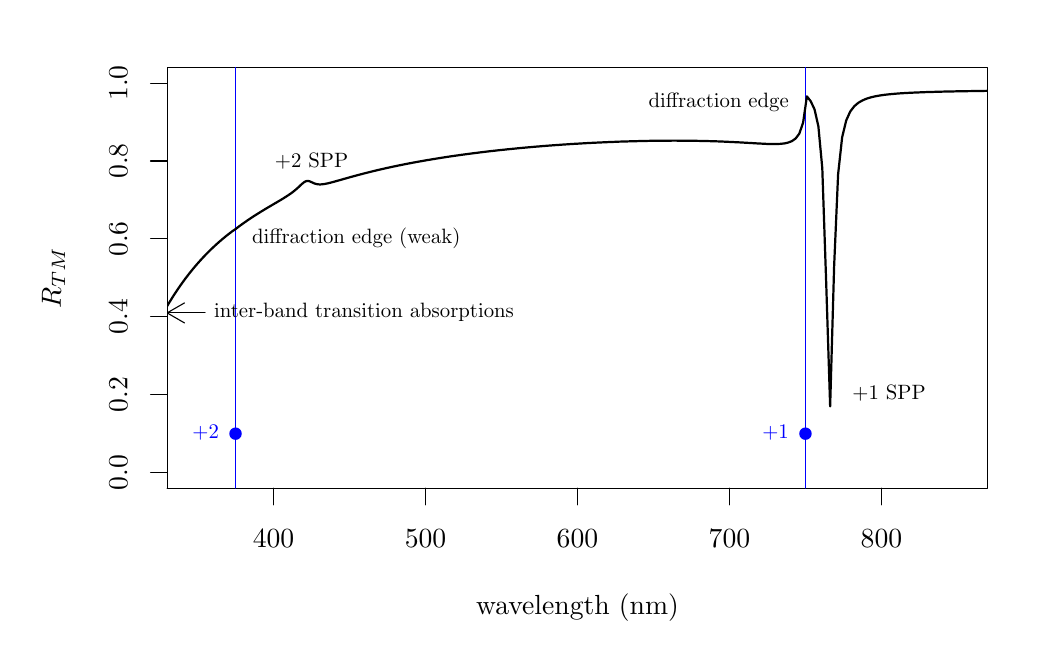
\begin{tikzpicture}[x=1pt,y=1pt]
\definecolor[named]{fillColor}{rgb}{1.00,1.00,1.00}
\path[use as bounding box,fill=fillColor,fill opacity=0.00] (0,0) rectangle (361.35,216.81);
\begin{scope}
\path[clip] (  0.00,  0.00) rectangle (361.35,216.81);
\definecolor[named]{drawColor}{rgb}{0.00,0.00,0.00}

\path[draw=drawColor,line width= 0.4pt,line join=round,line cap=round] ( 88.84, 50.40) -- (308.51, 50.40);

\path[draw=drawColor,line width= 0.4pt,line join=round,line cap=round] ( 88.84, 50.40) -- ( 88.84, 44.40);

\path[draw=drawColor,line width= 0.4pt,line join=round,line cap=round] (143.76, 50.40) -- (143.76, 44.40);

\path[draw=drawColor,line width= 0.4pt,line join=round,line cap=round] (198.67, 50.40) -- (198.67, 44.40);

\path[draw=drawColor,line width= 0.4pt,line join=round,line cap=round] (253.59, 50.40) -- (253.59, 44.40);

\path[draw=drawColor,line width= 0.4pt,line join=round,line cap=round] (308.51, 50.40) -- (308.51, 44.40);

\node[text=drawColor,anchor=base,inner sep=0pt, outer sep=0pt, scale=  1.00] at ( 88.84, 28.80) {400};

\node[text=drawColor,anchor=base,inner sep=0pt, outer sep=0pt, scale=  1.00] at (143.76, 28.80) {500};

\node[text=drawColor,anchor=base,inner sep=0pt, outer sep=0pt, scale=  1.00] at (198.67, 28.80) {600};

\node[text=drawColor,anchor=base,inner sep=0pt, outer sep=0pt, scale=  1.00] at (253.59, 28.80) {700};

\node[text=drawColor,anchor=base,inner sep=0pt, outer sep=0pt, scale=  1.00] at (308.51, 28.80) {800};

\path[draw=drawColor,line width= 0.4pt,line join=round,line cap=round] ( 50.40, 56.03) -- ( 50.40,196.78);

\path[draw=drawColor,line width= 0.4pt,line join=round,line cap=round] ( 50.40, 56.03) -- ( 44.40, 56.03);

\path[draw=drawColor,line width= 0.4pt,line join=round,line cap=round] ( 50.40, 84.18) -- ( 44.40, 84.18);

\path[draw=drawColor,line width= 0.4pt,line join=round,line cap=round] ( 50.40,112.33) -- ( 44.40,112.33);

\path[draw=drawColor,line width= 0.4pt,line join=round,line cap=round] ( 50.40,140.48) -- ( 44.40,140.48);

\path[draw=drawColor,line width= 0.4pt,line join=round,line cap=round] ( 50.40,168.63) -- ( 44.40,168.63);

\path[draw=drawColor,line width= 0.4pt,line join=round,line cap=round] ( 50.40,196.78) -- ( 44.40,196.78);

\node[text=drawColor,rotate= 90.00,anchor=base,inner sep=0pt, outer sep=0pt, scale=  1.00] at ( 36.00, 56.03) {0.0};

\node[text=drawColor,rotate= 90.00,anchor=base,inner sep=0pt, outer sep=0pt, scale=  1.00] at ( 36.00, 84.18) {0.2};

\node[text=drawColor,rotate= 90.00,anchor=base,inner sep=0pt, outer sep=0pt, scale=  1.00] at ( 36.00,112.33) {0.4};

\node[text=drawColor,rotate= 90.00,anchor=base,inner sep=0pt, outer sep=0pt, scale=  1.00] at ( 36.00,140.48) {0.6};

\node[text=drawColor,rotate= 90.00,anchor=base,inner sep=0pt, outer sep=0pt, scale=  1.00] at ( 36.00,168.63) {0.8};

\node[text=drawColor,rotate= 90.00,anchor=base,inner sep=0pt, outer sep=0pt, scale=  1.00] at ( 36.00,196.78) {1.0};

\path[draw=drawColor,line width= 0.4pt,line join=round,line cap=round] ( 50.40, 50.40) --
	(346.95, 50.40) --
	(346.95,202.41) --
	( 50.40,202.41) --
	( 50.40, 50.40);
\end{scope}
\begin{scope}
\path[clip] (  0.00,  0.00) rectangle (361.35,216.81);
\definecolor[named]{drawColor}{rgb}{0.00,0.00,0.00}

\node[text=drawColor,anchor=base,inner sep=0pt, outer sep=0pt, scale=  1.00] at (198.67,  4.80) {wavelength (nm)};

\node[text=drawColor,rotate= 90.00,anchor=base,inner sep=0pt, outer sep=0pt, scale=  1.00] at ( 12.00,126.41) {$R_{TM}$};
\end{scope}
\begin{scope}
\path[clip] ( 50.40, 50.40) rectangle (346.95,202.41);
\definecolor[named]{drawColor}{rgb}{0.00,0.00,1.00}

\path[draw=drawColor,line width= 0.4pt,line join=round,line cap=round] (281.05, 50.40) -- (281.05,202.41);

\path[draw=drawColor,line width= 0.4pt,line join=round,line cap=round] ( 75.11, 50.40) -- ( 75.11,202.41);
\definecolor[named]{drawColor}{rgb}{0.00,0.00,0.00}

\path[draw=drawColor,line width= 0.8pt,line join=round,line cap=round] (361.35,194.14) --
	(360.00,194.12) --
	(358.06,194.11) --
	(356.14,194.09) --
	(354.23,194.06) --
	(352.34,194.05) --
	(350.46,194.02) --
	(348.60,193.99) --
	(346.75,193.98) --
	(344.92,193.95) --
	(343.10,193.92) --
	(341.29,193.89) --
	(339.50,193.87) --
	(337.72,193.84) --
	(335.96,193.81) --
	(334.20,193.77) --
	(332.46,193.74) --
	(330.74,193.70) --
	(329.03,193.66) --
	(327.32,193.60) --
	(325.64,193.56) --
	(323.96,193.50) --
	(322.30,193.43) --
	(320.64,193.36) --
	(319.00,193.29) --
	(317.38,193.20) --
	(315.76,193.11) --
	(314.16,192.99) --
	(312.56,192.85) --
	(310.99,192.70) --
	(309.41,192.52) --
	(307.85,192.29) --
	(306.31,192.01) --
	(304.77,191.66) --
	(303.24,191.19) --
	(301.73,190.57) --
	(300.22,189.71) --
	(298.73,188.46) --
	(297.24,186.53) --
	(295.77,183.27) --
	(294.30,177.16) --
	(292.85,163.87) --
	(291.41,130.67) --
	(289.97, 79.94) --
	(288.55,124.34) --
	(287.13,166.03) --
	(285.72,181.16) --
	(284.33,187.29) --
	(282.94,190.25) --
	(281.57,191.98) --
	(280.20,182.49) --
	(278.84,178.54) --
	(277.49,176.75) --
	(276.15,175.81) --
	(274.81,175.29) --
	(273.49,174.99) --
	(272.18,174.84) --
	(270.87,174.77) --
	(269.57,174.75) --
	(268.28,174.77) --
	(267.00,174.81) --
	(265.72,174.88) --
	(264.46,174.94) --
	(263.20,175.01) --
	(261.95,175.09) --
	(260.71,175.16) --
	(259.48,175.23) --
	(258.25,175.30) --
	(257.03,175.37) --
	(255.82,175.43) --
	(254.62,175.48) --
	(253.42,175.54) --
	(252.24,175.60) --
	(251.05,175.65) --
	(249.88,175.70) --
	(248.72,175.74) --
	(247.56,175.78) --
	(246.40,175.81) --
	(245.26,175.84) --
	(244.12,175.86) --
	(242.99,175.89) --
	(241.86,175.91) --
	(240.75,175.93) --
	(239.63,175.95) --
	(238.53,175.96) --
	(237.43,175.98) --
	(236.34,175.98) --
	(235.25,175.98) --
	(234.17,175.99) --
	(233.10,175.99) --
	(232.04,175.98) --
	(230.98,175.98) --
	(229.92,175.98) --
	(228.87,175.96) --
	(227.84,175.95) --
	(226.80,175.93) --
	(225.77,175.92) --
	(224.74,175.91) --
	(223.73,175.89) --
	(222.72,175.86) --
	(221.71,175.85) --
	(220.71,175.82) --
	(219.71,175.79) --
	(218.73,175.77) --
	(217.74,175.74) --
	(216.76,175.71) --
	(215.79,175.68) --
	(214.83,175.65) --
	(213.86,175.63) --
	(212.90,175.58) --
	(211.95,175.54) --
	(211.01,175.51) --
	(210.07,175.47) --
	(209.13,175.43) --
	(208.20,175.39) --
	(207.27,175.34) --
	(206.36,175.30) --
	(205.44,175.26) --
	(204.53,175.22) --
	(203.62,175.17) --
	(202.72,175.12) --
	(201.83,175.08) --
	(200.94,175.02) --
	(200.05,174.98) --
	(199.17,174.92) --
	(198.29,174.87) --
	(197.42,174.82) --
	(196.56,174.77) --
	(195.69,174.71) --
	(194.83,174.65) --
	(193.98,174.60) --
	(193.13,174.54) --
	(192.28,174.47) --
	(191.44,174.41) --
	(190.61,174.36) --
	(189.77,174.30) --
	(188.95,174.23) --
	(188.13,174.18) --
	(187.31,174.11) --
	(186.49,174.05) --
	(185.68,173.98) --
	(184.87,173.91) --
	(184.07,173.85) --
	(183.27,173.78) --
	(182.47,173.71) --
	(181.69,173.64) --
	(180.90,173.57) --
	(180.12,173.50) --
	(179.34,173.43) --
	(178.56,173.36) --
	(177.80,173.29) --
	(177.03,173.22) --
	(176.26,173.13) --
	(175.51,173.06) --
	(174.75,172.99) --
	(174.00,172.91) --
	(173.25,172.84) --
	(172.50,172.75) --
	(171.76,172.68) --
	(171.02,172.60) --
	(170.29,172.53) --
	(169.56,172.44) --
	(168.83,172.36) --
	(168.11,172.28) --
	(167.39,172.21) --
	(166.68,172.12) --
	(165.96,172.04) --
	(165.25,171.95) --
	(164.55,171.87) --
	(163.85,171.78) --
	(163.14,171.70) --
	(162.45,171.60) --
	(161.75,171.52) --
	(161.07,171.43) --
	(160.38,171.35) --
	(159.70,171.25) --
	(159.02,171.16) --
	(158.34,171.08) --
	(157.67,170.98) --
	(157.00,170.90) --
	(156.33,170.80) --
	(155.66,170.70) --
	(155.01,170.61) --
	(154.35,170.52) --
	(153.69,170.42) --
	(153.04,170.33) --
	(152.39,170.23) --
	(151.74,170.14) --
	(151.10,170.04) --
	(150.46,169.94) --
	(149.83,169.84) --
	(149.19,169.74) --
	(148.56,169.64) --
	(147.93,169.54) --
	(147.31,169.43) --
	(146.68,169.33) --
	(146.06,169.24) --
	(145.44,169.12) --
	(144.83,169.02) --
	(144.21,168.93) --
	(143.61,168.81) --
	(143.00,168.71) --
	(142.40,168.60) --
	(141.80,168.49) --
	(141.20,168.39) --
	(140.60,168.28) --
	(140.01,168.17) --
	(139.41,168.07) --
	(138.83,167.95) --
	(138.24,167.84) --
	(137.66,167.73) --
	(137.08,167.62) --
	(136.50,167.50) --
	(135.93,167.39) --
	(135.35,167.28) --
	(134.78,167.15) --
	(134.21,167.04) --
	(133.65,166.93) --
	(133.08,166.81) --
	(132.52,166.69) --
	(131.96,166.58) --
	(131.41,166.45) --
	(130.85,166.34) --
	(130.30,166.21) --
	(129.75,166.10) --
	(129.21,165.97) --
	(128.66,165.84) --
	(128.12,165.72) --
	(127.58,165.60) --
	(127.04,165.48) --
	(126.50,165.35) --
	(125.97,165.22) --
	(125.44,165.10) --
	(124.91,164.97) --
	(124.38,164.84) --
	(123.86,164.70) --
	(123.33,164.58) --
	(122.82,164.45) --
	(122.30,164.32) --
	(121.78,164.18) --
	(121.27,164.06) --
	(120.75,163.91) --
	(120.24,163.79) --
	(119.74,163.65) --
	(119.23,163.52) --
	(118.73,163.38) --
	(118.23,163.25) --
	(117.73,163.11) --
	(117.23,162.97) --
	(116.73,162.85) --
	(116.24,162.70) --
	(115.75,162.56) --
	(115.26,162.42) --
	(114.77,162.28) --
	(114.28,162.16) --
	(113.80,162.01) --
	(113.32,161.87) --
	(112.84,161.73) --
	(112.36,161.61) --
	(111.88,161.47) --
	(111.41,161.34) --
	(110.93,161.20) --
	(110.46,161.07) --
	(110.00,160.95) --
	(109.53,160.82) --
	(109.06,160.71) --
	(108.60,160.59) --
	(108.14,160.49) --
	(107.68,160.40) --
	(107.22,160.31) --
	(106.76,160.26) --
	(106.31,160.20) --
	(105.85,160.17) --
	(105.40,160.17) --
	(104.95,160.20) --
	(104.50,160.27) --
	(104.06,160.38) --
	(103.61,160.52) --
	(103.17,160.71) --
	(102.73,160.92) --
	(102.29,161.11) --
	(101.85,161.30) --
	(101.42,161.40) --
	(100.98,161.41) --
	(100.55,161.31) --
	(100.12,161.11) --
	( 99.69,160.82) --
	( 99.26,160.47) --
	( 98.83,160.09) --
	( 98.41,159.69) --
	( 97.99,159.28) --
	( 97.56,158.90) --
	( 97.15,158.52) --
	( 96.72,158.16) --
	( 96.30,157.82) --
	( 95.89,157.50) --
	( 95.48,157.17) --
	( 95.06,156.88) --
	( 94.65,156.60) --
	( 94.25,156.31) --
	( 93.83,156.05) --
	( 93.43,155.78) --
	( 93.02,155.53) --
	( 92.62,155.27) --
	( 92.22,155.02) --
	( 91.82,154.78) --
	( 91.42,154.54) --
	( 91.02,154.30) --
	( 90.62,154.06) --
	( 90.23,153.84) --
	( 89.84,153.60) --
	( 89.44,153.37) --
	( 89.05,153.15) --
	( 88.66,152.92) --
	( 88.27,152.68) --
	( 87.89,152.46) --
	( 87.50,152.23) --
	( 87.12,152.01) --
	( 86.73,151.78) --
	( 86.35,151.56) --
	( 85.97,151.33) --
	( 85.59,151.11) --
	( 85.22,150.87) --
	( 84.84,150.64) --
	( 84.46,150.42) --
	( 84.09,150.19) --
	( 83.72,149.95) --
	( 83.35,149.73) --
	( 82.98,149.49) --
	( 82.61,149.26) --
	( 82.24,149.02) --
	( 81.88,148.80) --
	( 81.51,148.56) --
	( 81.15,148.32) --
	( 80.79,148.08) --
	( 80.42,147.84) --
	( 80.07,147.60) --
	( 79.71,147.36) --
	( 79.35,147.11) --
	( 79.00,146.87) --
	( 78.64,146.62) --
	( 78.29,146.38) --
	( 77.94,146.12) --
	( 77.58,145.87) --
	( 77.23,145.62) --
	( 76.88,145.36) --
	( 76.53,145.11) --
	( 76.19,144.86) --
	( 75.84,144.59) --
	( 75.50,144.34) --
	( 75.16,144.06) --
	( 74.82,143.84) --
	( 74.48,143.60) --
	( 74.13,143.37) --
	( 73.79,143.13) --
	( 73.46,142.87) --
	( 73.12,142.62) --
	( 72.78,142.35) --
	( 72.45,142.10) --
	( 72.12,141.83) --
	( 71.78,141.58) --
	( 71.46,141.31) --
	( 71.13,141.03) --
	( 70.80,140.76) --
	( 70.47,140.49) --
	( 70.14,140.21) --
	( 69.82,139.93) --
	( 69.49,139.66) --
	( 69.17,139.38) --
	( 68.85,139.09) --
	( 68.53,138.81) --
	( 68.20,138.52) --
	( 67.89,138.23) --
	( 67.57,137.93) --
	( 67.25,137.64) --
	( 66.94,137.34) --
	( 66.62,137.05) --
	( 66.30,136.74) --
	( 65.99,136.44) --
	( 65.68,136.13) --
	( 65.37,135.82) --
	( 65.06,135.51) --
	( 64.75,135.20) --
	( 64.44,134.88) --
	( 64.13,134.57) --
	( 63.83,134.24) --
	( 63.52,133.92) --
	( 63.22,133.60) --
	( 62.92,133.27) --
	( 62.61,132.94) --
	( 62.31,132.61) --
	( 62.01,132.27) --
	( 61.71,131.94) --
	( 61.41,131.60) --
	( 61.11,131.26) --
	( 60.82,130.91) --
	( 60.52,130.57) --
	( 60.22,130.22) --
	( 59.93,129.87) --
	( 59.64,129.52) --
	( 59.35,129.15) --
	( 59.05,128.80) --
	( 58.76,128.43) --
	( 58.47,128.07) --
	( 58.18,127.70) --
	( 57.90,127.33) --
	( 57.61,126.95) --
	( 57.32,126.59) --
	( 57.04,126.21) --
	( 56.75,125.83) --
	( 56.47,125.43) --
	( 56.19,125.05) --
	( 55.90,124.66) --
	( 55.62,124.27) --
	( 55.34,123.87) --
	( 55.06,123.48) --
	( 54.79,123.08) --
	( 54.51,122.68) --
	( 54.23,122.27) --
	( 53.95,121.86) --
	( 53.68,121.45) --
	( 53.40,121.03) --
	( 53.13,120.62) --
	( 52.86,120.20) --
	( 52.59,119.78) --
	( 52.32,119.35) --
	( 52.05,118.92) --
	( 51.78,118.48) --
	( 51.51,118.06) --
	( 51.24,117.62) --
	( 50.97,117.17) --
	( 50.71,116.74) --
	( 50.44,116.29) --
	( 50.17,115.83) --
	( 49.91,115.38) --
	( 49.65,114.93) --
	( 49.38,114.47) --
	( 49.13,114.02) --
	( 48.86,113.55) --
	( 48.60,113.08) --
	( 48.34,112.61) --
	( 48.08,112.15) --
	( 47.82,111.67) --
	( 47.57,111.19) --
	( 47.31,110.71) --
	( 47.06,110.23) --
	( 46.80,109.74) --
	( 46.54,109.26) --
	( 46.29,108.77) --
	( 46.04,108.28) --
	( 45.79,107.78) --
	( 45.53,107.28) --
	( 45.29,106.78) --
	( 45.03,106.28) --
	( 44.79,105.77) --
	( 44.54,105.26) --
	( 44.29,104.76) --
	( 44.04,104.24) --
	( 43.80,103.73) --
	( 43.55,103.21) --
	( 43.30,102.70) --
	( 43.06,102.18) --
	( 42.82,101.66) --
	( 42.57,101.13) --
	( 42.33,100.61) --
	( 42.09,100.08) --
	( 41.85, 99.55) --
	( 41.61, 99.03) --
	( 41.37, 98.49) --
	( 41.13, 97.96) --
	( 40.89, 97.44) --
	( 40.65, 96.90) --
	( 40.42, 96.37) --
	( 40.18, 95.83) --
	( 39.94, 95.30) --
	( 39.71, 94.76) --
	( 39.48, 94.23) --
	( 39.24, 93.69) --
	( 39.01, 93.16) --
	( 38.77, 92.62) --
	( 38.54, 92.09) --
	( 38.31, 91.56) --
	( 38.08, 91.02) --
	( 37.85, 90.49) --
	( 37.62, 89.96) --
	( 37.40, 89.43) --
	( 37.17, 88.91) --
	( 36.94, 88.37) --
	( 36.71, 87.85) --
	( 36.48, 87.33) --
	( 36.26, 86.81) --
	( 36.03, 86.29) --
	( 35.81, 85.77) --
	( 35.58, 85.26) --
	( 35.36, 84.74) --
	( 35.14, 84.24) --
	( 34.92, 83.74) --
	( 34.69, 83.24) --
	( 34.47, 82.74) --
	( 34.25, 82.25);
\definecolor[named]{fillColor}{rgb}{0.00,0.00,1.00}

\path[fill=fillColor] (281.05, 70.10) circle (  2.25);

\path[fill=fillColor] ( 75.11, 70.10) circle (  2.25);
\definecolor[named]{drawColor}{rgb}{0.00,0.00,1.00}

\node[text=drawColor,anchor=base east,inner sep=0pt, outer sep=0pt, scale=  0.75] at (275.05, 68.38) {$+1$};

\node[text=drawColor,anchor=base east,inner sep=0pt, outer sep=0pt, scale=  0.75] at ( 69.11, 68.38) {$+2$};
\definecolor[named]{drawColor}{rgb}{0.00,0.00,0.00}

\node[text=drawColor,anchor=base east,inner sep=0pt, outer sep=0pt, scale=  0.75] at (275.05,188.02) {diffraction edge};

\node[text=drawColor,anchor=base west,inner sep=0pt, outer sep=0pt, scale=  0.75] at (298.03, 82.46) {$+1$ SPP};

\node[text=drawColor,anchor=base west,inner sep=0pt, outer sep=0pt, scale=  0.75] at ( 67.38,112.02) {inter-band transition absorptions};

\path[draw=drawColor,line width= 0.4pt,line join=round,line cap=round] ( 64.13,113.74) -- ( 50.40,113.74);

\path[draw=drawColor,line width= 0.4pt,line join=round,line cap=round] ( 56.66,117.35) --
	( 50.40,113.74) --
	( 56.66,110.12);

\node[text=drawColor,anchor=base west,inner sep=0pt, outer sep=0pt, scale=  0.75] at ( 81.11,138.76) {diffraction edge (weak)};

\node[text=drawColor,anchor=base,inner sep=0pt, outer sep=0pt, scale=  0.75] at (102.57,166.18) {$+2$ SPP};
\end{scope}
\end{tikzpicture}

\end{center}
\caption[An example spectrum for a simple sinusoidal silver grating, calculated using the Chandezon method.]{An example spectrum for a simple sinusoidal silver grating, calculated using the Chandezon method. the grating has the following parameters: $\lambda_{gx}=750\:\nano\metre$, and depth of $40\:\nano\metre$ with a frequency dependent dielectric function for silver from literature \cite{Nash1996}. The spectra is taken at normal incidence with the polarisation perpendicular to the grating grooves.\label{fig:examplespectra}}
\end{figure}

Features of interest in this figure are labelled on the graph. The diffraction edge, the wavelength at which the first diffracting order begins to (or ceases to) propagate is clearly shown at $750\:\nano\metre$ as a sharp critical edge. Slightly higher in wavelength, at $\lambda_0\approx 765\:\nano\metre$, there is a sharp resonance in the reflectivity presenting as a minimum in the reflected light. This minimum is a result of the reflected light being out-of-phase with the light which is re-radiated from decaying SPPs.  The incident light is scattered by the grating and, when the coupling conditions are met, resonantly excites a SPP which travels along the surface. This SPP may then decay and scatter back into reflected light. A total of two scattering processes, an excitation and subsequent decay of a SPP, give the total phase change of the re-radiated light of $90^\circ+90^\circ+90^\circ+90^\circ=360^\circ$ relative to the incident light, while the reflected light which did not interact with the SPP has accumulated a total phase change of $180^\circ$ by the simple reflection from a metal surface. This results in the re-radiated light being out-of-phase with the reflected light by $180^\circ$, causing the observation of a minimum in reflection. Since no light is reflected, the energy is lost to Joule heating.

The position of the second order diffraction edge is marked on the spectrum, but is very weak. Beyond this diffraction edge, at $\lambda_0\approx 420\:\nano\metre$ there is a small resonance exhibited as a region of enhanced reflectivity, a `bright spot'. This is the result of reflected light being in-phase with the light re-radiated from the coupling of a $2^{nd}$ order SPP. The presentation of an optical interaction with a SPP as a maximum in the reflectivity is again a result of the phase difference accumulated from the scattering, coupling, and decay of light and the SPP. On a purely sinusoidal grating such as the one modelled here, multiple scattering processes are required to couple to this SPP, leading to the re-radiated light being in-phase with the non-interacting reflection. The waves constructively interfere, resulting in a maximum in the reflectivity coefficient.

The drop in the reflectivity at lower wavelengths is due to the metal's natural absorptions due to inter-band transitions and bulk plasmon excitations. The imaginary component of the metal's dielectric function at these wavelengths reflect these absorptions by becoming much larger. This `background' absorption can be seen in all the silver grating results in this thesis.



\subsection{Plasmonic Band Gaps}
When a propagating SPP encounters a counter-propagating SPP with equal energy and equal and opposite momentum, they will constructively interfere producing SPP standing waves \cite{Barnes1995,Barnes1996}. Typically, two possible SPP standing waves can occur, with the nodes and anti-nodes of one SPP standing wave shifted $\lambda/4$ in space with respect to the other, a typical result of any quantised standing waves confined to a single value of momentum. This is analogous to the well known physical examples of electron standing waves formed at Brillouin Zone (BZ) boundaries, or the vibrational modes of a solid rod.

On a flat surface, these two surface standing waves of electron density and coupled electromagnetic field are indistinguishable, save for the phase difference between them. They occur at the same energy and momentum as one another. On a diffraction grating the situation is quite different. The arrangements of charge along the shaped surface can result in the electron surface charge density sitting in very different electromagnetic potentials, for example at the bottom of a grating groove or at the top, which is depicted in figure \ref{fig:bandgapsCartoon}. In this case, the two possible standing waves have the same period (enforced by the periodic lattice) and so the same momentum, but will be associated with a different electromagnetic energy. Between these two energy values, SPP propagation is forbidden, due to destructive interference of the surface waves. An energy region of forbidden SPP propagation has been opened up, a plasmonic band-gap.  This is shown in the extended zone scheme dispersion plot in figure \ref{fig:bandgapsRadiativeA} which shows the Bragg scattering of SPPs at the first BZ boundary (at $k_g/2$) causing the formation of a band gap.

\begin{figure}
\begin{center}
\subfigure[]{
\def\svgwidth{0.45\linewidth}
\input{figure-bandgapcartoon1.pdf_tex}}
\subfigure[]{
\def\svgwidth{0.45\linewidth}
\input{figure-bandgapcartoon2.pdf_tex}}
\end{center}
\caption[Cartoon of two possible SPP standing waves on a sinusoidal grating.]{Cartoon of two possible SPP standing waves on a sinusoidal grating. The blue and red regions show accumulation of positive and negative charge density, respectively. These two standing waves, both which have a period of $2\lambda_g$, result in different field arrangements and so are associated with different energies.\label{fig:bandgapsCartoon}}
\end{figure}

The band gap shown in figure \ref{fig:bandgapsRadiativeA} will not be observed, as no available scattering event can diffract this region into the zero-order light cone. However, the band gap which occurs at the $2^{nd}$ BZ boundary may be, as shown in the repeated zone scheme dispersion in figure \ref{fig:bandgapsRadiativeB}\footnote{In this figure, the previous band gap at $k_x=k_g/2$ has been omitted for clarity.}. In this case, while a single $1k_g$ scattering event may bring the band gap region into the radiative zone, the interaction which leads to band gap formation is between a zero-order and the $2^{nd}$ order SPP at the $2^{nd}$ BZ boundary $(k_x=k_g)$. This means that the required scattering of the SPPs must be a $2k_g$ event for band gap formation. On purely sinusoidal gratings, which possess no  $2k_g$ component in their grating profile, this scattering process is mediated by multiple scattering events, which are very weak. Since this scattering amplitude for the SPP is so weak, the interference between counter-propagating modes will also be weak, and band gaps are unlikely to be large enough to be observed. If, however, the grating profile contains a $2k_g$ component (by, for example, the addition of a secondary pitch of the grating equal to half the period of the fundamental period), the SPPs may couple together to form a standing wave via a single strong scattering event. It is the $2k_g$ component that couples the SPPs together to form the band-gap, and the $1k_g$ component that scatters this into the radiative region and so may be observed, as shown in figure \ref{fig:bandgapsRadiativeB}.

\begin{figure}
\begin{center}
\subfigure[]{
\def\svgwidth{0.45\linewidth}
\input{figure-diffracted-bandgaps3.pdf_tex}\label{fig:bandgapsRadiativeA}}
\subfigure[]{
\def\svgwidth{0.45\linewidth}
\input{figure-diffracted-bandgaps2.pdf_tex}\label{fig:bandgapsRadiativeB}}
\end{center}
\caption[The dispersions and band gaps of a SPP on a grating with one Fourier Harmonic and on a grating with the first two Fourier Harmonics.]{The dispersion and band gap of (a) a SPP on a grating with one Fourier Harmonic and (b) on a grating with the first two Fourier Harmonics. The red line is the light line for free space light, the blue curves show the SPP contours. In (a) the black dotted line shown the unperturbed SPP contour, and the green dotted lines show the position of the first BZ.\label{fig:bandgapsRadiative}}
\end{figure}

Again, this is analogous to the formation of the electron band-structure of crystals, formed when considering nearly-free electrons in a periodic potential \cite{kittel1996introduction}, or photonic band-gaps in dielectric stacks/photonic crystals \cite{Search1993}. 

A subtle difference in the definition used in this thesis, and common in the research on surface plasmons, is that a `plasmonic band-gap' might only occur over a limited range of angles, whereas for electron band structure or photonic crystals a `band-gap' occurs in all possible propagation directions, and the term `stop-band' is used for single-direction gaps. Here, we adopt the convention of a band-gap occurring if an energy gap exists for which SPP propagation is forbidden over a given angle range, and reserve the term `full plasmonic band-gap' for forbidden SPP propagation for a range of frequencies in all directions.

\subsubsection{Coupling Light to Band Edges}
To scatter SPPs in to the radiative region and also couple the two SPP modes together to form standing waves requires suitable grating harmonics in the grating profile.  While the magnitude and position of the band gap is determined solely by the presence and size of these grating harmonics, the coupling of light to the SPP standing waves depends strongly on the relative phase between the grating components. We can demonstrate this simply by considering the band gap which will open at normal incidence ($\theta=0^\circ$) for  a grating described by the simple Fourier sum,
\begin{equation*}
f(x)=A_1\sin(k_g x)+A_2\sin(2k_g x + \psi_2)
\end{equation*}
where, in our case, $A_1=5\:\nano\metre$, $A_2=2\:\nano\metre$, $k_g=2\pi/\lambda_g$ where $\lambda_g=605\:\nano\metre$. $\varepsilon = -17.5 + 0.7i $. $\psi_2$ is the relative phase of the $2k_g$ component relative to the $k_g$  component. Three reflectivity plots as a function of angular frequency and in-plane momentum around the band gap  region are shown on the right side of figure \ref{fig:couplingbandedges}, with each plot showing the numerically calculated reflectivity for different values of $\psi_2$. The method used for calculation is the Chandezon method \cite{Chandezon1980,Li1999}, detailed later in chapter \ref{c:theorymethods}.
\begin{figure}
\begin{center}
\subfigure[$\psi_2=0^\circ$]{% Created by tikzDevice version 0.6.2-92-0ad2792 on 2013-01-22 18:38:21
% !TEX encoding = UTF-8 Unicode
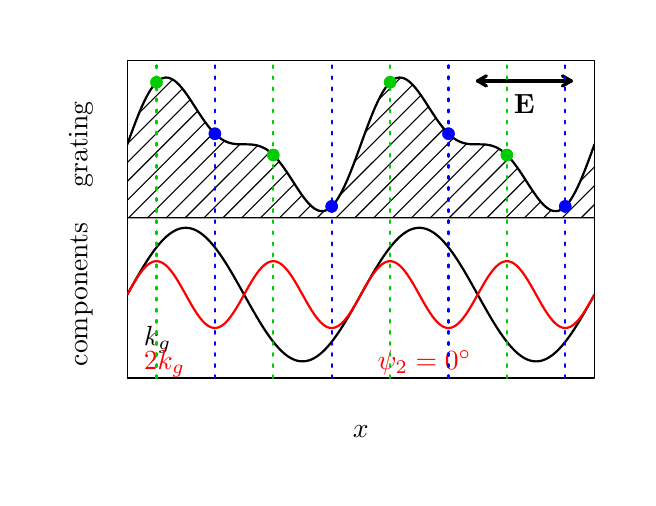
\begin{tikzpicture}[x=1pt,y=1pt]
\definecolor[named]{fillColor}{rgb}{1.00,1.00,1.00}
\path[use as bounding box,fill=fillColor,fill opacity=0.00] (0,0) rectangle (216.81,162.61);
\begin{scope}
\path[clip] ( 36.00, 36.00) rectangle (204.81,150.61);
\definecolor[named]{drawColor}{rgb}{0.00,0.00,0.00}

\path[draw=drawColor,line width= 0.8pt,line join=round,line cap=round] ( 36.00,120.45) --
	( 36.34,121.38) --
	( 36.68,122.32) --
	( 37.01,123.25) --
	( 37.35,124.17) --
	( 37.69,125.09) --
	( 38.03,126.01) --
	( 38.37,126.91) --
	( 38.71,127.81) --
	( 39.04,128.69) --
	( 39.38,129.56) --
	( 39.72,130.41) --
	( 40.06,131.25) --
	( 40.40,132.08) --
	( 40.74,132.88) --
	( 41.07,133.67) --
	( 41.41,134.43) --
	( 41.75,135.17) --
	( 42.09,135.89) --
	( 42.43,136.59) --
	( 42.77,137.26) --
	( 43.10,137.91) --
	( 43.44,138.53) --
	( 43.78,139.12) --
	( 44.12,139.69) --
	( 44.46,140.22) --
	( 44.80,140.73) --
	( 45.13,141.21) --
	( 45.47,141.65) --
	( 45.81,142.07) --
	( 46.15,142.45) --
	( 46.49,142.81) --
	( 46.83,143.13) --
	( 47.16,143.42) --
	( 47.50,143.67) --
	( 47.84,143.90) --
	( 48.18,144.09) --
	( 48.52,144.25) --
	( 48.86,144.38) --
	( 49.19,144.47) --
	( 49.53,144.54) --
	( 49.87,144.57) --
	( 50.21,144.57) --
	( 50.55,144.55) --
	( 50.89,144.49) --
	( 51.22,144.40) --
	( 51.56,144.28) --
	( 51.90,144.14) --
	( 52.24,143.97) --
	( 52.58,143.77) --
	( 52.91,143.55) --
	( 53.25,143.30) --
	( 53.59,143.03) --
	( 53.93,142.73) --
	( 54.27,142.41) --
	( 54.61,142.07) --
	( 54.94,141.71) --
	( 55.28,141.34) --
	( 55.62,140.94) --
	( 55.96,140.53) --
	( 56.30,140.10) --
	( 56.64,139.65) --
	( 56.97,139.20) --
	( 57.31,138.73) --
	( 57.65,138.25) --
	( 57.99,137.76) --
	( 58.33,137.26) --
	( 58.67,136.75) --
	( 59.00,136.24) --
	( 59.34,135.72) --
	( 59.68,135.20) --
	( 60.02,134.68) --
	( 60.36,134.15) --
	( 60.70,133.62) --
	( 61.03,133.10) --
	( 61.37,132.58) --
	( 61.71,132.05) --
	( 62.05,131.54) --
	( 62.39,131.02) --
	( 62.73,130.52) --
	( 63.06,130.02) --
	( 63.40,129.53) --
	( 63.74,129.04) --
	( 64.08,128.57) --
	( 64.42,128.10) --
	( 64.76,127.65) --
	( 65.09,127.21) --
	( 65.43,126.78) --
	( 65.77,126.36) --
	( 66.11,125.96) --
	( 66.45,125.57) --
	( 66.78,125.19) --
	( 67.12,124.83) --
	( 67.46,124.48) --
	( 67.80,124.15) --
	( 68.14,123.83) --
	( 68.48,123.53) --
	( 68.81,123.25) --
	( 69.15,122.98) --
	( 69.49,122.72) --
	( 69.83,122.49) --
	( 70.17,122.26) --
	( 70.51,122.06) --
	( 70.84,121.86) --
	( 71.18,121.68) --
	( 71.52,121.52) --
	( 71.86,121.37) --
	( 72.20,121.24) --
	( 72.54,121.11) --
	( 72.87,121.00) --
	( 73.21,120.91) --
	( 73.55,120.82) --
	( 73.89,120.75) --
	( 74.23,120.68) --
	( 74.57,120.63) --
	( 74.90,120.58) --
	( 75.24,120.55) --
	( 75.58,120.52) --
	( 75.92,120.49) --
	( 76.26,120.48) --
	( 76.60,120.46) --
	( 76.93,120.46) --
	( 77.27,120.45) --
	( 77.61,120.45) --
	( 77.95,120.45) --
	( 78.29,120.45) --
	( 78.63,120.45) --
	( 78.96,120.45) --
	( 79.30,120.44) --
	( 79.64,120.44) --
	( 79.98,120.43) --
	( 80.32,120.41) --
	( 80.66,120.39) --
	( 80.99,120.37) --
	( 81.33,120.33) --
	( 81.67,120.29) --
	( 82.01,120.24) --
	( 82.35,120.18) --
	( 82.68,120.11) --
	( 83.02,120.03) --
	( 83.36,119.94) --
	( 83.70,119.84) --
	( 84.04,119.72) --
	( 84.38,119.59) --
	( 84.71,119.45) --
	( 85.05,119.29) --
	( 85.39,119.12) --
	( 85.73,118.94) --
	( 86.07,118.74) --
	( 86.41,118.52) --
	( 86.74,118.29) --
	( 87.08,118.05) --
	( 87.42,117.78) --
	( 87.76,117.51) --
	( 88.10,117.21) --
	( 88.44,116.90) --
	( 88.77,116.58) --
	( 89.11,116.24) --
	( 89.45,115.89) --
	( 89.79,115.52) --
	( 90.13,115.13) --
	( 90.47,114.74) --
	( 90.80,114.33) --
	( 91.14,113.90) --
	( 91.48,113.47) --
	( 91.82,113.02) --
	( 92.16,112.56) --
	( 92.50,112.09) --
	( 92.83,111.61) --
	( 93.17,111.12) --
	( 93.51,110.63) --
	( 93.85,110.12) --
	( 94.19,109.61) --
	( 94.53,109.10) --
	( 94.86,108.58) --
	( 95.20,108.06) --
	( 95.54,107.53) --
	( 95.88,107.01) --
	( 96.22,106.48) --
	( 96.56,105.96) --
	( 96.89,105.43) --
	( 97.23,104.91) --
	( 97.57,104.40) --
	( 97.91,103.89) --
	( 98.25,103.39) --
	( 98.58,102.89) --
	( 98.92,102.41) --
	( 99.26,101.93) --
	( 99.60,101.47) --
	( 99.94,101.02) --
	(100.28,100.58) --
	(100.61,100.16) --
	(100.95, 99.76) --
	(101.29, 99.37) --
	(101.63, 99.00) --
	(101.97, 98.65) --
	(102.31, 98.32) --
	(102.64, 98.01) --
	(102.98, 97.73) --
	(103.32, 97.47) --
	(103.66, 97.23) --
	(104.00, 97.02) --
	(104.34, 96.84) --
	(104.67, 96.68) --
	(105.01, 96.55) --
	(105.35, 96.45) --
	(105.69, 96.38) --
	(106.03, 96.33) --
	(106.37, 96.32) --
	(106.70, 96.34) --
	(107.04, 96.39) --
	(107.38, 96.47) --
	(107.72, 96.58) --
	(108.06, 96.72) --
	(108.40, 96.90) --
	(108.73, 97.11) --
	(109.07, 97.35) --
	(109.41, 97.62) --
	(109.75, 97.93) --
	(110.09, 98.26) --
	(110.43, 98.63) --
	(110.76, 99.03) --
	(111.10, 99.46) --
	(111.44, 99.92) --
	(111.78,100.41) --
	(112.12,100.94) --
	(112.46,101.49) --
	(112.79,102.07) --
	(113.13,102.67) --
	(113.47,103.31) --
	(113.81,103.97) --
	(114.15,104.65) --
	(114.48,105.36) --
	(114.82,106.09) --
	(115.16,106.84) --
	(115.50,107.62) --
	(115.84,108.41) --
	(116.18,109.23) --
	(116.51,110.06) --
	(116.85,110.91) --
	(117.19,111.77) --
	(117.53,112.65) --
	(117.87,113.54) --
	(118.21,114.43) --
	(118.54,115.34) --
	(118.88,116.26) --
	(119.22,117.18) --
	(119.56,118.11) --
	(119.90,119.05) --
	(120.24,119.98) --
	(120.57,120.92) --
	(120.91,121.85) --
	(121.25,122.78) --
	(121.59,123.71) --
	(121.93,124.63) --
	(122.27,125.55) --
	(122.60,126.46) --
	(122.94,127.36) --
	(123.28,128.25) --
	(123.62,129.12) --
	(123.96,129.99) --
	(124.30,130.84) --
	(124.63,131.67) --
	(124.97,132.48) --
	(125.31,133.28) --
	(125.65,134.05) --
	(125.99,134.80) --
	(126.33,135.54) --
	(126.66,136.25) --
	(127.00,136.93) --
	(127.34,137.59) --
	(127.68,138.22) --
	(128.02,138.83) --
	(128.35,139.41) --
	(128.69,139.96) --
	(129.03,140.48) --
	(129.37,140.97) --
	(129.71,141.43) --
	(130.05,141.86) --
	(130.38,142.26) --
	(130.72,142.63) --
	(131.06,142.97) --
	(131.40,143.27) --
	(131.74,143.55) --
	(132.08,143.79) --
	(132.41,144.00) --
	(132.75,144.17) --
	(133.09,144.32) --
	(133.43,144.43) --
	(133.77,144.51) --
	(134.11,144.56) --
	(134.44,144.58) --
	(134.78,144.56) --
	(135.12,144.52) --
	(135.46,144.45) --
	(135.80,144.35) --
	(136.14,144.22) --
	(136.47,144.06) --
	(136.81,143.87) --
	(137.15,143.66) --
	(137.49,143.43) --
	(137.83,143.17) --
	(138.17,142.88) --
	(138.50,142.57) --
	(138.84,142.24) --
	(139.18,141.90) --
	(139.52,141.53) --
	(139.86,141.14) --
	(140.20,140.73) --
	(140.53,140.31) --
	(140.87,139.88) --
	(141.21,139.43) --
	(141.55,138.96) --
	(141.89,138.49) --
	(142.23,138.00) --
	(142.56,137.51) --
	(142.90,137.01) --
	(143.24,136.50) --
	(143.58,135.98) --
	(143.92,135.46) --
	(144.25,134.94) --
	(144.59,134.41) --
	(144.93,133.89) --
	(145.27,133.36) --
	(145.61,132.84) --
	(145.95,132.31) --
	(146.28,131.80) --
	(146.62,131.28) --
	(146.96,130.77) --
	(147.30,130.27) --
	(147.64,129.77) --
	(147.98,129.28) --
	(148.31,128.80) --
	(148.65,128.33) --
	(148.99,127.88) --
	(149.33,127.43) --
	(149.67,126.99) --
	(150.01,126.57) --
	(150.34,126.16) --
	(150.68,125.76) --
	(151.02,125.38) --
	(151.36,125.01) --
	(151.70,124.65) --
	(152.04,124.32) --
	(152.37,123.99) --
	(152.71,123.68) --
	(153.05,123.39) --
	(153.39,123.11) --
	(153.73,122.85) --
	(154.07,122.60) --
	(154.40,122.37) --
	(154.74,122.16) --
	(155.08,121.96) --
	(155.42,121.77) --
	(155.76,121.60) --
	(156.10,121.44) --
	(156.43,121.30) --
	(156.77,121.17) --
	(157.11,121.06) --
	(157.45,120.95) --
	(157.79,120.86) --
	(158.13,120.78) --
	(158.46,120.71) --
	(158.80,120.65) --
	(159.14,120.60) --
	(159.48,120.56) --
	(159.82,120.53) --
	(160.15,120.50) --
	(160.49,120.48) --
	(160.83,120.47) --
	(161.17,120.46) --
	(161.51,120.45) --
	(161.85,120.45) --
	(162.18,120.45) --
	(162.52,120.45) --
	(162.86,120.45) --
	(163.20,120.45) --
	(163.54,120.44) --
	(163.88,120.44) --
	(164.21,120.43) --
	(164.55,120.42) --
	(164.89,120.40) --
	(165.23,120.38) --
	(165.57,120.35) --
	(165.91,120.31) --
	(166.24,120.27) --
	(166.58,120.21) --
	(166.92,120.15) --
	(167.26,120.07) --
	(167.60,119.99) --
	(167.94,119.89) --
	(168.27,119.78) --
	(168.61,119.66) --
	(168.95,119.52) --
	(169.29,119.37) --
	(169.63,119.21) --
	(169.97,119.03) --
	(170.30,118.84) --
	(170.64,118.63) --
	(170.98,118.41) --
	(171.32,118.17) --
	(171.66,117.92) --
	(172.00,117.65) --
	(172.33,117.36) --
	(172.67,117.06) --
	(173.01,116.74) --
	(173.35,116.41) --
	(173.69,116.07) --
	(174.03,115.70) --
	(174.36,115.33) --
	(174.70,114.94) --
	(175.04,114.53) --
	(175.38,114.12) --
	(175.72,113.69) --
	(176.05,113.24) --
	(176.39,112.79) --
	(176.73,112.33) --
	(177.07,111.85) --
	(177.41,111.37) --
	(177.75,110.88) --
	(178.08,110.38) --
	(178.42,109.87) --
	(178.76,109.36) --
	(179.10,108.84) --
	(179.44,108.32) --
	(179.78,107.80) --
	(180.11,107.27) --
	(180.45,106.74) --
	(180.79,106.22) --
	(181.13,105.69) --
	(181.47,105.17) --
	(181.81,104.66) --
	(182.14,104.14) --
	(182.48,103.64) --
	(182.82,103.14) --
	(183.16,102.65) --
	(183.50,102.17) --
	(183.84,101.70) --
	(184.17,101.24) --
	(184.51,100.80) --
	(184.85,100.37) --
	(185.19, 99.96) --
	(185.53, 99.56) --
	(185.87, 99.18) --
	(186.20, 98.82) --
	(186.54, 98.48) --
	(186.88, 98.17) --
	(187.22, 97.87) --
	(187.56, 97.60) --
	(187.90, 97.35) --
	(188.23, 97.12) --
	(188.57, 96.93) --
	(188.91, 96.75) --
	(189.25, 96.61) --
	(189.59, 96.49) --
	(189.92, 96.41) --
	(190.26, 96.35) --
	(190.60, 96.32) --
	(190.94, 96.32) --
	(191.28, 96.36) --
	(191.62, 96.42) --
	(191.95, 96.52) --
	(192.29, 96.65) --
	(192.63, 96.81) --
	(192.97, 97.00) --
	(193.31, 97.22) --
	(193.65, 97.48) --
	(193.98, 97.77) --
	(194.32, 98.09) --
	(194.66, 98.44) --
	(195.00, 98.83) --
	(195.34, 99.24) --
	(195.68, 99.69) --
	(196.01,100.17) --
	(196.35,100.67) --
	(196.69,101.21) --
	(197.03,101.77) --
	(197.37,102.37) --
	(197.71,102.99) --
	(198.04,103.63) --
	(198.38,104.30) --
	(198.72,105.00) --
	(199.06,105.72) --
	(199.40,106.46) --
	(199.74,107.23) --
	(200.07,108.01) --
	(200.41,108.82) --
	(200.75,109.64) --
	(201.09,110.48) --
	(201.43,111.34) --
	(201.77,112.21) --
	(202.10,113.09) --
	(202.44,113.98) --
	(202.78,114.89) --
	(203.12,115.80) --
	(203.46,116.72) --
	(203.80,117.65) --
	(204.13,118.58) --
	(204.47,119.51) --
	(204.81,120.45);
\end{scope}
\begin{scope}
\path[clip] (  0.00,  0.00) rectangle (216.81,162.61);
\definecolor[named]{drawColor}{rgb}{0.00,0.00,0.00}

\path[draw=drawColor,line width= 0.4pt,line join=round,line cap=round] ( 36.00, 36.00) --
	(204.81, 36.00) --
	(204.81,150.61) --
	( 36.00,150.61) --
	( 36.00, 36.00);
\end{scope}
\begin{scope}
\path[clip] (  0.00,  0.00) rectangle (216.81,162.61);
\definecolor[named]{drawColor}{rgb}{0.00,0.00,0.00}

\node[text=drawColor,rotate= 90.00,anchor=base,inner sep=0pt, outer sep=0pt, scale=  1.00] at ( 21.60,120.45) {grating};

\node[text=drawColor,rotate= 90.00,anchor=base,inner sep=0pt, outer sep=0pt, scale=  1.00] at ( 21.60, 66.16) {components};

\node[text=drawColor,anchor=base,inner sep=0pt, outer sep=0pt, scale=  1.00] at (120.41, 14.40) {$x$};
\end{scope}
\begin{scope}
\path[clip] ( 36.00, 36.00) rectangle (204.81,150.61);
\definecolor[named]{drawColor}{rgb}{0.00,0.00,0.00}

\node[text=drawColor,anchor=base west,inner sep=0pt, outer sep=0pt, scale=  1.00] at ( 42.00, 47.94) {$k_g$};
\definecolor[named]{drawColor}{rgb}{1.00,0.00,0.00}

\node[text=drawColor,anchor=base west,inner sep=0pt, outer sep=0pt, scale=  1.00] at ( 42.00, 39.25) {2$k_g$};

\node[text=drawColor,anchor=base west,inner sep=0pt, outer sep=0pt, scale=  1.00] at (126.41, 39.25) {$\psi_2=0^\circ$};
\definecolor[named]{drawColor}{rgb}{0.00,0.00,0.00}

\path[draw=drawColor,line width= 1.2pt,line join=round,line cap=round] (162.61,143.37) -- (196.37,143.37);

\path[draw=drawColor,line width= 1.2pt,line join=round,line cap=round] (165.74,145.18) --
	(162.61,143.37) --
	(165.74,141.56);

\path[draw=drawColor,line width= 1.2pt,line join=round,line cap=round] (193.24,141.56) --
	(196.37,143.37) --
	(193.24,145.18);

\node[text=drawColor,anchor=base,inner sep=0pt, outer sep=0pt, scale=  1.00] at (179.49,131.63) {$\mathbf{E}$};

\path[draw=drawColor,line width= 0.4pt,line join=round,line cap=round] ( 40.26,131.74) -- ( 52.39,143.88);

\path[draw=drawColor,line width= 0.4pt,line join=round,line cap=round] ( 36.13,120.79) -- ( 55.91,140.58);

\path[draw=drawColor,line width= 0.4pt,line join=round,line cap=round] ( 36.00,113.86) -- ( 58.76,136.61);

\path[draw=drawColor,line width= 0.4pt,line join=round,line cap=round] ( 36.00,107.04) -- ( 61.44,132.48);

\path[draw=drawColor,line width= 0.4pt,line join=round,line cap=round] ( 36.00,100.23) -- ( 64.19,128.42);

\path[draw=drawColor,line width= 0.4pt,line join=round,line cap=round] ( 36.49, 93.91) -- ( 67.27,124.68);

\path[draw=drawColor,line width= 0.4pt,line join=round,line cap=round] ( 43.31, 93.91) -- ( 71.12,121.72);

\path[draw=drawColor,line width= 0.4pt,line join=round,line cap=round] ( 50.12, 93.91) -- ( 76.67,120.46);

\path[draw=drawColor,line width= 0.4pt,line join=round,line cap=round] ( 56.93, 93.91) -- ( 83.05,120.02);

\path[draw=drawColor,line width= 0.4pt,line join=round,line cap=round] ( 63.75, 93.91) -- ( 87.53,117.69);

\path[draw=drawColor,line width= 0.4pt,line join=round,line cap=round] ( 70.56, 93.91) -- ( 90.88,114.23);

\path[draw=drawColor,line width= 0.4pt,line join=round,line cap=round] ( 77.37, 93.91) -- ( 93.75,110.28);

\path[draw=drawColor,line width= 0.4pt,line join=round,line cap=round] ( 84.19, 93.91) -- ( 96.43,106.15);

\path[draw=drawColor,line width= 0.4pt,line join=round,line cap=round] (126.80,136.52) -- (134.84,144.56);

\path[draw=drawColor,line width= 0.4pt,line join=round,line cap=round] ( 91.00, 93.91) -- ( 99.16,102.07);

\path[draw=drawColor,line width= 0.4pt,line join=round,line cap=round] (122.04,124.95) -- (139.09,141.99);

\path[draw=drawColor,line width= 0.4pt,line join=round,line cap=round] ( 97.82, 93.91) -- (102.27, 98.36);

\path[draw=drawColor,line width= 0.4pt,line join=round,line cap=round] (118.12,114.21) -- (142.10,138.19);

\path[draw=drawColor,line width= 0.4pt,line join=round,line cap=round] (104.63, 93.91) -- (107.13, 96.41);

\path[draw=drawColor,line width= 0.4pt,line join=round,line cap=round] (112.80,102.08) -- (144.81,134.08);

\path[draw=drawColor,line width= 0.4pt,line join=round,line cap=round] (111.44, 93.91) -- (147.50,129.97);

\path[draw=drawColor,line width= 0.4pt,line join=round,line cap=round] (118.26, 93.91) -- (150.42,126.07);

\path[draw=drawColor,line width= 0.4pt,line join=round,line cap=round] (125.07, 93.91) -- (153.89,122.73);

\path[draw=drawColor,line width= 0.4pt,line join=round,line cap=round] (131.88, 93.91) -- (158.66,120.68);

\path[draw=drawColor,line width= 0.4pt,line join=round,line cap=round] (138.70, 93.91) -- (165.17,120.38);

\path[draw=drawColor,line width= 0.4pt,line join=round,line cap=round] (145.51, 93.91) -- (170.39,118.79);

\path[draw=drawColor,line width= 0.4pt,line join=round,line cap=round] (152.32, 93.91) -- (174.07,115.65);

\path[draw=drawColor,line width= 0.4pt,line join=round,line cap=round] (159.14, 93.91) -- (177.08,111.84);

\path[draw=drawColor,line width= 0.4pt,line join=round,line cap=round] (165.95, 93.91) -- (179.80,107.76);

\path[draw=drawColor,line width= 0.4pt,line join=round,line cap=round] (172.77, 93.91) -- (182.49,103.63);

\path[draw=drawColor,line width= 0.4pt,line join=round,line cap=round] (179.58, 93.91) -- (185.39, 99.72);

\path[draw=drawColor,line width= 0.4pt,line join=round,line cap=round] (204.07,118.39) -- (205.05,119.37);

\path[draw=drawColor,line width= 0.4pt,line join=round,line cap=round] (186.39, 93.91) -- (189.14, 96.66);

\path[draw=drawColor,line width= 0.4pt,line join=round,line cap=round] (199.75,107.26) -- (206.27,113.79);

\path[draw=drawColor,line width= 0.4pt,line join=round,line cap=round] (193.21, 93.91) -- (207.50,108.20);

\path[draw=drawColor,line width= 0.4pt,line join=round,line cap=round] (200.02, 93.91) -- (208.72,102.61);

\path[draw=drawColor,line width= 0.4pt,line join=round,line cap=round] (206.83, 93.91) -- (209.95, 97.02);

\path[draw=drawColor,line width= 0.4pt,line join=round,line cap=round] ( 36.00,120.45) --
	( 36.34,121.38) --
	( 36.68,122.32) --
	( 37.01,123.25) --
	( 37.35,124.17) --
	( 37.69,125.09) --
	( 38.03,126.01) --
	( 38.37,126.91) --
	( 38.71,127.81) --
	( 39.04,128.69) --
	( 39.38,129.56) --
	( 39.72,130.41) --
	( 40.06,131.25) --
	( 40.40,132.08) --
	( 40.74,132.88) --
	( 41.07,133.67) --
	( 41.41,134.43) --
	( 41.75,135.17) --
	( 42.09,135.89) --
	( 42.43,136.59) --
	( 42.77,137.26) --
	( 43.10,137.91) --
	( 43.44,138.53) --
	( 43.78,139.12) --
	( 44.12,139.69) --
	( 44.46,140.22) --
	( 44.80,140.73) --
	( 45.13,141.21) --
	( 45.47,141.65) --
	( 45.81,142.07) --
	( 46.15,142.45) --
	( 46.49,142.81) --
	( 46.83,143.13) --
	( 47.16,143.42) --
	( 47.50,143.67) --
	( 47.84,143.90) --
	( 48.18,144.09) --
	( 48.52,144.25) --
	( 48.86,144.38) --
	( 49.19,144.47) --
	( 49.53,144.54) --
	( 49.87,144.57) --
	( 50.21,144.57) --
	( 50.55,144.55) --
	( 50.89,144.49) --
	( 51.22,144.40) --
	( 51.56,144.28) --
	( 51.90,144.14) --
	( 52.24,143.97) --
	( 52.58,143.77) --
	( 52.91,143.55) --
	( 53.25,143.30) --
	( 53.59,143.03) --
	( 53.93,142.73) --
	( 54.27,142.41) --
	( 54.61,142.07) --
	( 54.94,141.71) --
	( 55.28,141.34) --
	( 55.62,140.94) --
	( 55.96,140.53) --
	( 56.30,140.10) --
	( 56.64,139.65) --
	( 56.97,139.20) --
	( 57.31,138.73) --
	( 57.65,138.25) --
	( 57.99,137.76) --
	( 58.33,137.26) --
	( 58.67,136.75) --
	( 59.00,136.24) --
	( 59.34,135.72) --
	( 59.68,135.20) --
	( 60.02,134.68) --
	( 60.36,134.15) --
	( 60.70,133.62) --
	( 61.03,133.10) --
	( 61.37,132.58) --
	( 61.71,132.05) --
	( 62.05,131.54) --
	( 62.39,131.02) --
	( 62.73,130.52) --
	( 63.06,130.02) --
	( 63.40,129.53) --
	( 63.74,129.04) --
	( 64.08,128.57) --
	( 64.42,128.10) --
	( 64.76,127.65) --
	( 65.09,127.21) --
	( 65.43,126.78) --
	( 65.77,126.36) --
	( 66.11,125.96) --
	( 66.45,125.57) --
	( 66.78,125.19) --
	( 67.12,124.83) --
	( 67.46,124.48) --
	( 67.80,124.15) --
	( 68.14,123.83) --
	( 68.48,123.53) --
	( 68.81,123.25) --
	( 69.15,122.98) --
	( 69.49,122.72) --
	( 69.83,122.49) --
	( 70.17,122.26) --
	( 70.51,122.06) --
	( 70.84,121.86) --
	( 71.18,121.68) --
	( 71.52,121.52) --
	( 71.86,121.37) --
	( 72.20,121.24) --
	( 72.54,121.11) --
	( 72.87,121.00) --
	( 73.21,120.91) --
	( 73.55,120.82) --
	( 73.89,120.75) --
	( 74.23,120.68) --
	( 74.57,120.63) --
	( 74.90,120.58) --
	( 75.24,120.55) --
	( 75.58,120.52) --
	( 75.92,120.49) --
	( 76.26,120.48) --
	( 76.60,120.46) --
	( 76.93,120.46) --
	( 77.27,120.45) --
	( 77.61,120.45) --
	( 77.95,120.45) --
	( 78.29,120.45) --
	( 78.63,120.45) --
	( 78.96,120.45) --
	( 79.30,120.44) --
	( 79.64,120.44) --
	( 79.98,120.43) --
	( 80.32,120.41) --
	( 80.66,120.39) --
	( 80.99,120.37) --
	( 81.33,120.33) --
	( 81.67,120.29) --
	( 82.01,120.24) --
	( 82.35,120.18) --
	( 82.68,120.11) --
	( 83.02,120.03) --
	( 83.36,119.94) --
	( 83.70,119.84) --
	( 84.04,119.72) --
	( 84.38,119.59) --
	( 84.71,119.45) --
	( 85.05,119.29) --
	( 85.39,119.12) --
	( 85.73,118.94) --
	( 86.07,118.74) --
	( 86.41,118.52) --
	( 86.74,118.29) --
	( 87.08,118.05) --
	( 87.42,117.78) --
	( 87.76,117.51) --
	( 88.10,117.21) --
	( 88.44,116.90) --
	( 88.77,116.58) --
	( 89.11,116.24) --
	( 89.45,115.89) --
	( 89.79,115.52) --
	( 90.13,115.13) --
	( 90.47,114.74) --
	( 90.80,114.33) --
	( 91.14,113.90) --
	( 91.48,113.47) --
	( 91.82,113.02) --
	( 92.16,112.56) --
	( 92.50,112.09) --
	( 92.83,111.61) --
	( 93.17,111.12) --
	( 93.51,110.63) --
	( 93.85,110.12) --
	( 94.19,109.61) --
	( 94.53,109.10) --
	( 94.86,108.58) --
	( 95.20,108.06) --
	( 95.54,107.53) --
	( 95.88,107.01) --
	( 96.22,106.48) --
	( 96.56,105.96) --
	( 96.89,105.43) --
	( 97.23,104.91) --
	( 97.57,104.40) --
	( 97.91,103.89) --
	( 98.25,103.39) --
	( 98.58,102.89) --
	( 98.92,102.41) --
	( 99.26,101.93) --
	( 99.60,101.47) --
	( 99.94,101.02) --
	(100.28,100.58) --
	(100.61,100.16) --
	(100.95, 99.76) --
	(101.29, 99.37) --
	(101.63, 99.00) --
	(101.97, 98.65) --
	(102.31, 98.32) --
	(102.64, 98.01) --
	(102.98, 97.73) --
	(103.32, 97.47) --
	(103.66, 97.23) --
	(104.00, 97.02) --
	(104.34, 96.84) --
	(104.67, 96.68) --
	(105.01, 96.55) --
	(105.35, 96.45) --
	(105.69, 96.38) --
	(106.03, 96.33) --
	(106.37, 96.32) --
	(106.70, 96.34) --
	(107.04, 96.39) --
	(107.38, 96.47) --
	(107.72, 96.58) --
	(108.06, 96.72) --
	(108.40, 96.90) --
	(108.73, 97.11) --
	(109.07, 97.35) --
	(109.41, 97.62) --
	(109.75, 97.93) --
	(110.09, 98.26) --
	(110.43, 98.63) --
	(110.76, 99.03) --
	(111.10, 99.46) --
	(111.44, 99.92) --
	(111.78,100.41) --
	(112.12,100.94) --
	(112.46,101.49) --
	(112.79,102.07) --
	(113.13,102.67) --
	(113.47,103.31) --
	(113.81,103.97) --
	(114.15,104.65) --
	(114.48,105.36) --
	(114.82,106.09) --
	(115.16,106.84) --
	(115.50,107.62) --
	(115.84,108.41) --
	(116.18,109.23) --
	(116.51,110.06) --
	(116.85,110.91) --
	(117.19,111.77) --
	(117.53,112.65) --
	(117.87,113.54) --
	(118.21,114.43) --
	(118.54,115.34) --
	(118.88,116.26) --
	(119.22,117.18) --
	(119.56,118.11) --
	(119.90,119.05) --
	(120.24,119.98) --
	(120.57,120.92) --
	(120.91,121.85) --
	(121.25,122.78) --
	(121.59,123.71) --
	(121.93,124.63) --
	(122.27,125.55) --
	(122.60,126.46) --
	(122.94,127.36) --
	(123.28,128.25) --
	(123.62,129.12) --
	(123.96,129.99) --
	(124.30,130.84) --
	(124.63,131.67) --
	(124.97,132.48) --
	(125.31,133.28) --
	(125.65,134.05) --
	(125.99,134.80) --
	(126.33,135.54) --
	(126.66,136.25) --
	(127.00,136.93) --
	(127.34,137.59) --
	(127.68,138.22) --
	(128.02,138.83) --
	(128.35,139.41) --
	(128.69,139.96) --
	(129.03,140.48) --
	(129.37,140.97) --
	(129.71,141.43) --
	(130.05,141.86) --
	(130.38,142.26) --
	(130.72,142.63) --
	(131.06,142.97) --
	(131.40,143.27) --
	(131.74,143.55) --
	(132.08,143.79) --
	(132.41,144.00) --
	(132.75,144.17) --
	(133.09,144.32) --
	(133.43,144.43) --
	(133.77,144.51) --
	(134.11,144.56) --
	(134.44,144.58) --
	(134.78,144.56) --
	(135.12,144.52) --
	(135.46,144.45) --
	(135.80,144.35) --
	(136.14,144.22) --
	(136.47,144.06) --
	(136.81,143.87) --
	(137.15,143.66) --
	(137.49,143.43) --
	(137.83,143.17) --
	(138.17,142.88) --
	(138.50,142.57) --
	(138.84,142.24) --
	(139.18,141.90) --
	(139.52,141.53) --
	(139.86,141.14) --
	(140.20,140.73) --
	(140.53,140.31) --
	(140.87,139.88) --
	(141.21,139.43) --
	(141.55,138.96) --
	(141.89,138.49) --
	(142.23,138.00) --
	(142.56,137.51) --
	(142.90,137.01) --
	(143.24,136.50) --
	(143.58,135.98) --
	(143.92,135.46) --
	(144.25,134.94) --
	(144.59,134.41) --
	(144.93,133.89) --
	(145.27,133.36) --
	(145.61,132.84) --
	(145.95,132.31) --
	(146.28,131.80) --
	(146.62,131.28) --
	(146.96,130.77) --
	(147.30,130.27) --
	(147.64,129.77) --
	(147.98,129.28) --
	(148.31,128.80) --
	(148.65,128.33) --
	(148.99,127.88) --
	(149.33,127.43) --
	(149.67,126.99) --
	(150.01,126.57) --
	(150.34,126.16) --
	(150.68,125.76) --
	(151.02,125.38) --
	(151.36,125.01) --
	(151.70,124.65) --
	(152.04,124.32) --
	(152.37,123.99) --
	(152.71,123.68) --
	(153.05,123.39) --
	(153.39,123.11) --
	(153.73,122.85) --
	(154.07,122.60) --
	(154.40,122.37) --
	(154.74,122.16) --
	(155.08,121.96) --
	(155.42,121.77) --
	(155.76,121.60) --
	(156.10,121.44) --
	(156.43,121.30) --
	(156.77,121.17) --
	(157.11,121.06) --
	(157.45,120.95) --
	(157.79,120.86) --
	(158.13,120.78) --
	(158.46,120.71) --
	(158.80,120.65) --
	(159.14,120.60) --
	(159.48,120.56) --
	(159.82,120.53) --
	(160.15,120.50) --
	(160.49,120.48) --
	(160.83,120.47) --
	(161.17,120.46) --
	(161.51,120.45) --
	(161.85,120.45) --
	(162.18,120.45) --
	(162.52,120.45) --
	(162.86,120.45) --
	(163.20,120.45) --
	(163.54,120.44) --
	(163.88,120.44) --
	(164.21,120.43) --
	(164.55,120.42) --
	(164.89,120.40) --
	(165.23,120.38) --
	(165.57,120.35) --
	(165.91,120.31) --
	(166.24,120.27) --
	(166.58,120.21) --
	(166.92,120.15) --
	(167.26,120.07) --
	(167.60,119.99) --
	(167.94,119.89) --
	(168.27,119.78) --
	(168.61,119.66) --
	(168.95,119.52) --
	(169.29,119.37) --
	(169.63,119.21) --
	(169.97,119.03) --
	(170.30,118.84) --
	(170.64,118.63) --
	(170.98,118.41) --
	(171.32,118.17) --
	(171.66,117.92) --
	(172.00,117.65) --
	(172.33,117.36) --
	(172.67,117.06) --
	(173.01,116.74) --
	(173.35,116.41) --
	(173.69,116.07) --
	(174.03,115.70) --
	(174.36,115.33) --
	(174.70,114.94) --
	(175.04,114.53) --
	(175.38,114.12) --
	(175.72,113.69) --
	(176.05,113.24) --
	(176.39,112.79) --
	(176.73,112.33) --
	(177.07,111.85) --
	(177.41,111.37) --
	(177.75,110.88) --
	(178.08,110.38) --
	(178.42,109.87) --
	(178.76,109.36) --
	(179.10,108.84) --
	(179.44,108.32) --
	(179.78,107.80) --
	(180.11,107.27) --
	(180.45,106.74) --
	(180.79,106.22) --
	(181.13,105.69) --
	(181.47,105.17) --
	(181.81,104.66) --
	(182.14,104.14) --
	(182.48,103.64) --
	(182.82,103.14) --
	(183.16,102.65) --
	(183.50,102.17) --
	(183.84,101.70) --
	(184.17,101.24) --
	(184.51,100.80) --
	(184.85,100.37) --
	(185.19, 99.96) --
	(185.53, 99.56) --
	(185.87, 99.18) --
	(186.20, 98.82) --
	(186.54, 98.48) --
	(186.88, 98.17) --
	(187.22, 97.87) --
	(187.56, 97.60) --
	(187.90, 97.35) --
	(188.23, 97.12) --
	(188.57, 96.93) --
	(188.91, 96.75) --
	(189.25, 96.61) --
	(189.59, 96.49) --
	(189.92, 96.41) --
	(190.26, 96.35) --
	(190.60, 96.32) --
	(190.94, 96.32) --
	(191.28, 96.36) --
	(191.62, 96.42) --
	(191.95, 96.52) --
	(192.29, 96.65) --
	(192.63, 96.81) --
	(192.97, 97.00) --
	(193.31, 97.22) --
	(193.65, 97.48) --
	(193.98, 97.77) --
	(194.32, 98.09) --
	(194.66, 98.44) --
	(195.00, 98.83) --
	(195.34, 99.24) --
	(195.68, 99.69) --
	(196.01,100.17) --
	(196.35,100.67) --
	(196.69,101.21) --
	(197.03,101.77) --
	(197.37,102.37) --
	(197.71,102.99) --
	(198.04,103.63) --
	(198.38,104.30) --
	(198.72,105.00) --
	(199.06,105.72) --
	(199.40,106.46) --
	(199.74,107.23) --
	(200.07,108.01) --
	(200.41,108.82) --
	(200.75,109.64) --
	(201.09,110.48) --
	(201.43,111.34) --
	(201.77,112.21) --
	(202.10,113.09) --
	(202.44,113.98) --
	(202.78,114.89) --
	(203.12,115.80) --
	(203.46,116.72) --
	(203.80,117.65) --
	(204.13,118.58) --
	(204.47,119.51) --
	(204.81,120.45) --
	(210.64, 93.91) --
	( 36.00, 93.91) --
	( 36.00,120.45);

\path[draw=drawColor,line width= 0.8pt,line join=round,line cap=round] ( 36.00, 66.16) --
	( 36.34, 66.77) --
	( 36.68, 67.37) --
	( 37.01, 67.98) --
	( 37.35, 68.59) --
	( 37.69, 69.19) --
	( 38.03, 69.79) --
	( 38.37, 70.39) --
	( 38.71, 70.99) --
	( 39.04, 71.58) --
	( 39.38, 72.17) --
	( 39.72, 72.76) --
	( 40.06, 73.34) --
	( 40.40, 73.92) --
	( 40.74, 74.49) --
	( 41.07, 75.06) --
	( 41.41, 75.62) --
	( 41.75, 76.18) --
	( 42.09, 76.73) --
	( 42.43, 77.27) --
	( 42.77, 77.80) --
	( 43.10, 78.33) --
	( 43.44, 78.85) --
	( 43.78, 79.37) --
	( 44.12, 79.87) --
	( 44.46, 80.37) --
	( 44.80, 80.85) --
	( 45.13, 81.33) --
	( 45.47, 81.80) --
	( 45.81, 82.26) --
	( 46.15, 82.70) --
	( 46.49, 83.14) --
	( 46.83, 83.57) --
	( 47.16, 83.98) --
	( 47.50, 84.39) --
	( 47.84, 84.78) --
	( 48.18, 85.16) --
	( 48.52, 85.53) --
	( 48.86, 85.88) --
	( 49.19, 86.23) --
	( 49.53, 86.56) --
	( 49.87, 86.88) --
	( 50.21, 87.18) --
	( 50.55, 87.47) --
	( 50.89, 87.75) --
	( 51.22, 88.01) --
	( 51.56, 88.27) --
	( 51.90, 88.50) --
	( 52.24, 88.72) --
	( 52.58, 88.93) --
	( 52.91, 89.13) --
	( 53.25, 89.30) --
	( 53.59, 89.47) --
	( 53.93, 89.62) --
	( 54.27, 89.75) --
	( 54.61, 89.87) --
	( 54.94, 89.98) --
	( 55.28, 90.07) --
	( 55.62, 90.14) --
	( 55.96, 90.20) --
	( 56.30, 90.24) --
	( 56.64, 90.27) --
	( 56.97, 90.29) --
	( 57.31, 90.28) --
	( 57.65, 90.27) --
	( 57.99, 90.24) --
	( 58.33, 90.19) --
	( 58.67, 90.12) --
	( 59.00, 90.05) --
	( 59.34, 89.95) --
	( 59.68, 89.84) --
	( 60.02, 89.72) --
	( 60.36, 89.58) --
	( 60.70, 89.43) --
	( 61.03, 89.26) --
	( 61.37, 89.08) --
	( 61.71, 88.88) --
	( 62.05, 88.67) --
	( 62.39, 88.44) --
	( 62.73, 88.20) --
	( 63.06, 87.95) --
	( 63.40, 87.68) --
	( 63.74, 87.40) --
	( 64.08, 87.11) --
	( 64.42, 86.80) --
	( 64.76, 86.48) --
	( 65.09, 86.14) --
	( 65.43, 85.80) --
	( 65.77, 85.44) --
	( 66.11, 85.06) --
	( 66.45, 84.68) --
	( 66.78, 84.29) --
	( 67.12, 83.88) --
	( 67.46, 83.46) --
	( 67.80, 83.03) --
	( 68.14, 82.59) --
	( 68.48, 82.14) --
	( 68.81, 81.68) --
	( 69.15, 81.21) --
	( 69.49, 80.73) --
	( 69.83, 80.24) --
	( 70.17, 79.75) --
	( 70.51, 79.24) --
	( 70.84, 78.72) --
	( 71.18, 78.20) --
	( 71.52, 77.67) --
	( 71.86, 77.13) --
	( 72.20, 76.59) --
	( 72.54, 76.04) --
	( 72.87, 75.48) --
	( 73.21, 74.92) --
	( 73.55, 74.35) --
	( 73.89, 73.77) --
	( 74.23, 73.20) --
	( 74.57, 72.61) --
	( 74.90, 72.02) --
	( 75.24, 71.43) --
	( 75.58, 70.84) --
	( 75.92, 70.24) --
	( 76.26, 69.64) --
	( 76.60, 69.04) --
	( 76.93, 68.44) --
	( 77.27, 67.83) --
	( 77.61, 67.22) --
	( 77.95, 66.62) --
	( 78.29, 66.01) --
	( 78.63, 65.40) --
	( 78.96, 64.79) --
	( 79.30, 64.19) --
	( 79.64, 63.58) --
	( 79.98, 62.98) --
	( 80.32, 62.38) --
	( 80.66, 61.78) --
	( 80.99, 61.18) --
	( 81.33, 60.59) --
	( 81.67, 60.00) --
	( 82.01, 59.42) --
	( 82.35, 58.83) --
	( 82.68, 58.26) --
	( 83.02, 57.69) --
	( 83.36, 57.12) --
	( 83.70, 56.56) --
	( 84.04, 56.01) --
	( 84.38, 55.46) --
	( 84.71, 54.92) --
	( 85.05, 54.38) --
	( 85.39, 53.86) --
	( 85.73, 53.34) --
	( 86.07, 52.83) --
	( 86.41, 52.32) --
	( 86.74, 51.83) --
	( 87.08, 51.35) --
	( 87.42, 50.87) --
	( 87.76, 50.41) --
	( 88.10, 49.95) --
	( 88.44, 49.51) --
	( 88.77, 49.07) --
	( 89.11, 48.65) --
	( 89.45, 48.24) --
	( 89.79, 47.84) --
	( 90.13, 47.45) --
	( 90.47, 47.07) --
	( 90.80, 46.70) --
	( 91.14, 46.35) --
	( 91.48, 46.01) --
	( 91.82, 45.68) --
	( 92.16, 45.37) --
	( 92.50, 45.06) --
	( 92.83, 44.78) --
	( 93.17, 44.50) --
	( 93.51, 44.24) --
	( 93.85, 43.99) --
	( 94.19, 43.76) --
	( 94.53, 43.54) --
	( 94.86, 43.34) --
	( 95.20, 43.15) --
	( 95.54, 42.97) --
	( 95.88, 42.81) --
	( 96.22, 42.67) --
	( 96.56, 42.54) --
	( 96.89, 42.42) --
	( 97.23, 42.32) --
	( 97.57, 42.23) --
	( 97.91, 42.16) --
	( 98.25, 42.11) --
	( 98.58, 42.07) --
	( 98.92, 42.04) --
	( 99.26, 42.03) --
	( 99.60, 42.04) --
	( 99.94, 42.06) --
	(100.28, 42.10) --
	(100.61, 42.15) --
	(100.95, 42.21) --
	(101.29, 42.30) --
	(101.63, 42.39) --
	(101.97, 42.50) --
	(102.31, 42.63) --
	(102.64, 42.77) --
	(102.98, 42.93) --
	(103.32, 43.10) --
	(103.66, 43.29) --
	(104.00, 43.49) --
	(104.34, 43.71) --
	(104.67, 43.93) --
	(105.01, 44.18) --
	(105.35, 44.44) --
	(105.69, 44.71) --
	(106.03, 44.99) --
	(106.37, 45.29) --
	(106.70, 45.60) --
	(107.04, 45.93) --
	(107.38, 46.26) --
	(107.72, 46.61) --
	(108.06, 46.98) --
	(108.40, 47.35) --
	(108.73, 47.74) --
	(109.07, 48.13) --
	(109.41, 48.54) --
	(109.75, 48.97) --
	(110.09, 49.40) --
	(110.43, 49.84) --
	(110.76, 50.29) --
	(111.10, 50.75) --
	(111.44, 51.23) --
	(111.78, 51.71) --
	(112.12, 52.20) --
	(112.46, 52.70) --
	(112.79, 53.21) --
	(113.13, 53.73) --
	(113.47, 54.25) --
	(113.81, 54.78) --
	(114.15, 55.32) --
	(114.48, 55.87) --
	(114.82, 56.42) --
	(115.16, 56.98) --
	(115.50, 57.54) --
	(115.84, 58.11) --
	(116.18, 58.69) --
	(116.51, 59.27) --
	(116.85, 59.85) --
	(117.19, 60.44) --
	(117.53, 61.03) --
	(117.87, 61.63) --
	(118.21, 62.23) --
	(118.54, 62.83) --
	(118.88, 63.43) --
	(119.22, 64.04) --
	(119.56, 64.64) --
	(119.90, 65.25) --
	(120.24, 65.86) --
	(120.57, 66.46) --
	(120.91, 67.07) --
	(121.25, 67.68) --
	(121.59, 68.28) --
	(121.93, 68.89) --
	(122.27, 69.49) --
	(122.60, 70.09) --
	(122.94, 70.69) --
	(123.28, 71.29) --
	(123.62, 71.88) --
	(123.96, 72.47) --
	(124.30, 73.05) --
	(124.63, 73.63) --
	(124.97, 74.21) --
	(125.31, 74.78) --
	(125.65, 75.34) --
	(125.99, 75.90) --
	(126.33, 76.45) --
	(126.66, 77.00) --
	(127.00, 77.54) --
	(127.34, 78.07) --
	(127.68, 78.59) --
	(128.02, 79.11) --
	(128.35, 79.62) --
	(128.69, 80.12) --
	(129.03, 80.61) --
	(129.37, 81.09) --
	(129.71, 81.57) --
	(130.05, 82.03) --
	(130.38, 82.48) --
	(130.72, 82.92) --
	(131.06, 83.35) --
	(131.40, 83.78) --
	(131.74, 84.18) --
	(132.08, 84.58) --
	(132.41, 84.97) --
	(132.75, 85.34) --
	(133.09, 85.71) --
	(133.43, 86.06) --
	(133.77, 86.39) --
	(134.11, 86.72) --
	(134.44, 87.03) --
	(134.78, 87.33) --
	(135.12, 87.61) --
	(135.46, 87.88) --
	(135.80, 88.14) --
	(136.14, 88.39) --
	(136.47, 88.61) --
	(136.81, 88.83) --
	(137.15, 89.03) --
	(137.49, 89.22) --
	(137.83, 89.39) --
	(138.17, 89.55) --
	(138.50, 89.69) --
	(138.84, 89.81) --
	(139.18, 89.93) --
	(139.52, 90.02) --
	(139.86, 90.11) --
	(140.20, 90.17) --
	(140.53, 90.22) --
	(140.87, 90.26) --
	(141.21, 90.28) --
	(141.55, 90.29) --
	(141.89, 90.28) --
	(142.23, 90.25) --
	(142.56, 90.21) --
	(142.90, 90.16) --
	(143.24, 90.09) --
	(143.58, 90.00) --
	(143.92, 89.90) --
	(144.25, 89.78) --
	(144.59, 89.65) --
	(144.93, 89.51) --
	(145.27, 89.35) --
	(145.61, 89.17) --
	(145.95, 88.98) --
	(146.28, 88.78) --
	(146.62, 88.56) --
	(146.96, 88.33) --
	(147.30, 88.08) --
	(147.64, 87.82) --
	(147.98, 87.54) --
	(148.31, 87.25) --
	(148.65, 86.95) --
	(148.99, 86.64) --
	(149.33, 86.31) --
	(149.67, 85.97) --
	(150.01, 85.62) --
	(150.34, 85.25) --
	(150.68, 84.87) --
	(151.02, 84.48) --
	(151.36, 84.08) --
	(151.70, 83.67) --
	(152.04, 83.25) --
	(152.37, 82.81) --
	(152.71, 82.37) --
	(153.05, 81.91) --
	(153.39, 81.45) --
	(153.73, 80.97) --
	(154.07, 80.49) --
	(154.40, 80.00) --
	(154.74, 79.49) --
	(155.08, 78.98) --
	(155.42, 78.46) --
	(155.76, 77.94) --
	(156.10, 77.40) --
	(156.43, 76.86) --
	(156.77, 76.31) --
	(157.11, 75.76) --
	(157.45, 75.20) --
	(157.79, 74.63) --
	(158.13, 74.06) --
	(158.46, 73.49) --
	(158.80, 72.90) --
	(159.14, 72.32) --
	(159.48, 71.73) --
	(159.82, 71.14) --
	(160.15, 70.54) --
	(160.49, 69.94) --
	(160.83, 69.34) --
	(161.17, 68.74) --
	(161.51, 68.13) --
	(161.85, 67.53) --
	(162.18, 66.92) --
	(162.52, 66.31) --
	(162.86, 65.70) --
	(163.20, 65.10) --
	(163.54, 64.49) --
	(163.88, 63.88) --
	(164.21, 63.28) --
	(164.55, 62.68) --
	(164.89, 62.08) --
	(165.23, 61.48) --
	(165.57, 60.89) --
	(165.91, 60.29) --
	(166.24, 59.71) --
	(166.58, 59.12) --
	(166.92, 58.55) --
	(167.26, 57.97) --
	(167.60, 57.40) --
	(167.94, 56.84) --
	(168.27, 56.28) --
	(168.61, 55.73) --
	(168.95, 55.19) --
	(169.29, 54.65) --
	(169.63, 54.12) --
	(169.97, 53.60) --
	(170.30, 53.08) --
	(170.64, 52.57) --
	(170.98, 52.08) --
	(171.32, 51.59) --
	(171.66, 51.11) --
	(172.00, 50.64) --
	(172.33, 50.18) --
	(172.67, 49.73) --
	(173.01, 49.29) --
	(173.35, 48.86) --
	(173.69, 48.44) --
	(174.03, 48.03) --
	(174.36, 47.64) --
	(174.70, 47.26) --
	(175.04, 46.88) --
	(175.38, 46.52) --
	(175.72, 46.18) --
	(176.05, 45.84) --
	(176.39, 45.52) --
	(176.73, 45.21) --
	(177.07, 44.92) --
	(177.41, 44.64) --
	(177.75, 44.37) --
	(178.08, 44.12) --
	(178.42, 43.88) --
	(178.76, 43.65) --
	(179.10, 43.44) --
	(179.44, 43.24) --
	(179.78, 43.06) --
	(180.11, 42.89) --
	(180.45, 42.74) --
	(180.79, 42.60) --
	(181.13, 42.48) --
	(181.47, 42.37) --
	(181.81, 42.27) --
	(182.14, 42.20) --
	(182.48, 42.13) --
	(182.82, 42.08) --
	(183.16, 42.05) --
	(183.50, 42.03) --
	(183.84, 42.03) --
	(184.17, 42.05) --
	(184.51, 42.08) --
	(184.85, 42.12) --
	(185.19, 42.18) --
	(185.53, 42.25) --
	(185.87, 42.34) --
	(186.20, 42.45) --
	(186.54, 42.57) --
	(186.88, 42.70) --
	(187.22, 42.85) --
	(187.56, 43.02) --
	(187.90, 43.19) --
	(188.23, 43.39) --
	(188.57, 43.60) --
	(188.91, 43.82) --
	(189.25, 44.05) --
	(189.59, 44.31) --
	(189.92, 44.57) --
	(190.26, 44.85) --
	(190.60, 45.14) --
	(190.94, 45.44) --
	(191.28, 45.76) --
	(191.62, 46.09) --
	(191.95, 46.44) --
	(192.29, 46.79) --
	(192.63, 47.16) --
	(192.97, 47.54) --
	(193.31, 47.93) --
	(193.65, 48.34) --
	(193.98, 48.75) --
	(194.32, 49.18) --
	(194.66, 49.62) --
	(195.00, 50.06) --
	(195.34, 50.52) --
	(195.68, 50.99) --
	(196.01, 51.47) --
	(196.35, 51.95) --
	(196.69, 52.45) --
	(197.03, 52.95) --
	(197.37, 53.47) --
	(197.71, 53.99) --
	(198.04, 54.51) --
	(198.38, 55.05) --
	(198.72, 55.59) --
	(199.06, 56.14) --
	(199.40, 56.70) --
	(199.74, 57.26) --
	(200.07, 57.83) --
	(200.41, 58.40) --
	(200.75, 58.98) --
	(201.09, 59.56) --
	(201.43, 60.15) --
	(201.77, 60.74) --
	(202.10, 61.33) --
	(202.44, 61.93) --
	(202.78, 62.53) --
	(203.12, 63.13) --
	(203.46, 63.73) --
	(203.80, 64.34) --
	(204.13, 64.95) --
	(204.47, 65.55) --
	(204.81, 66.16);
\definecolor[named]{drawColor}{rgb}{1.00,0.00,0.00}

\path[draw=drawColor,line width= 0.8pt,line join=round,line cap=round] ( 36.00, 66.16) --
	( 36.34, 66.77) --
	( 36.68, 67.37) --
	( 37.01, 67.98) --
	( 37.35, 68.57) --
	( 37.69, 69.17) --
	( 38.03, 69.75) --
	( 38.37, 70.33) --
	( 38.71, 70.89) --
	( 39.04, 71.44) --
	( 39.38, 71.98) --
	( 39.72, 72.51) --
	( 40.06, 73.02) --
	( 40.40, 73.51) --
	( 40.74, 73.98) --
	( 41.07, 74.43) --
	( 41.41, 74.86) --
	( 41.75, 75.27) --
	( 42.09, 75.66) --
	( 42.43, 76.02) --
	( 42.77, 76.36) --
	( 43.10, 76.67) --
	( 43.44, 76.96) --
	( 43.78, 77.21) --
	( 44.12, 77.44) --
	( 44.46, 77.64) --
	( 44.80, 77.81) --
	( 45.13, 77.96) --
	( 45.47, 78.07) --
	( 45.81, 78.15) --
	( 46.15, 78.20) --
	( 46.49, 78.22) --
	( 46.83, 78.21) --
	( 47.16, 78.17) --
	( 47.50, 78.10) --
	( 47.84, 78.00) --
	( 48.18, 77.87) --
	( 48.52, 77.71) --
	( 48.86, 77.52) --
	( 49.19, 77.30) --
	( 49.53, 77.05) --
	( 49.87, 76.78) --
	( 50.21, 76.48) --
	( 50.55, 76.15) --
	( 50.89, 75.80) --
	( 51.22, 75.42) --
	( 51.56, 75.02) --
	( 51.90, 74.60) --
	( 52.24, 74.15) --
	( 52.58, 73.69) --
	( 52.91, 73.20) --
	( 53.25, 72.70) --
	( 53.59, 72.18) --
	( 53.93, 71.65) --
	( 54.27, 71.10) --
	( 54.61, 70.54) --
	( 54.94, 69.97) --
	( 55.28, 69.39) --
	( 55.62, 68.80) --
	( 55.96, 68.20) --
	( 56.30, 67.60) --
	( 56.64, 66.99) --
	( 56.97, 66.39) --
	( 57.31, 65.78) --
	( 57.65, 65.17) --
	( 57.99, 64.57) --
	( 58.33, 63.97) --
	( 58.67, 63.37) --
	( 59.00, 62.79) --
	( 59.34, 62.21) --
	( 59.68, 61.64) --
	( 60.02, 61.08) --
	( 60.36, 60.54) --
	( 60.70, 60.01) --
	( 61.03, 59.49) --
	( 61.37, 59.00) --
	( 61.71, 58.52) --
	( 62.05, 58.06) --
	( 62.39, 57.62) --
	( 62.73, 57.20) --
	( 63.06, 56.80) --
	( 63.40, 56.43) --
	( 63.74, 56.08) --
	( 64.08, 55.76) --
	( 64.42, 55.47) --
	( 64.76, 55.20) --
	( 65.09, 54.96) --
	( 65.43, 54.75) --
	( 65.77, 54.57) --
	( 66.11, 54.41) --
	( 66.45, 54.29) --
	( 66.78, 54.20) --
	( 67.12, 54.13) --
	( 67.46, 54.10) --
	( 67.80, 54.10) --
	( 68.14, 54.13) --
	( 68.48, 54.19) --
	( 68.81, 54.28) --
	( 69.15, 54.40) --
	( 69.49, 54.55) --
	( 69.83, 54.72) --
	( 70.17, 54.93) --
	( 70.51, 55.17) --
	( 70.84, 55.43) --
	( 71.18, 55.72) --
	( 71.52, 56.04) --
	( 71.86, 56.39) --
	( 72.20, 56.76) --
	( 72.54, 57.15) --
	( 72.87, 57.56) --
	( 73.21, 58.00) --
	( 73.55, 58.46) --
	( 73.89, 58.93) --
	( 74.23, 59.43) --
	( 74.57, 59.94) --
	( 74.90, 60.47) --
	( 75.24, 61.01) --
	( 75.58, 61.57) --
	( 75.92, 62.14) --
	( 76.26, 62.71) --
	( 76.60, 63.30) --
	( 76.93, 63.89) --
	( 77.27, 64.49) --
	( 77.61, 65.10) --
	( 77.95, 65.70) --
	( 78.29, 66.31) --
	( 78.63, 66.92) --
	( 78.96, 67.52) --
	( 79.30, 68.13) --
	( 79.64, 68.72) --
	( 79.98, 69.31) --
	( 80.32, 69.90) --
	( 80.66, 70.47) --
	( 80.99, 71.03) --
	( 81.33, 71.58) --
	( 81.67, 72.11) --
	( 82.01, 72.64) --
	( 82.35, 73.14) --
	( 82.68, 73.63) --
	( 83.02, 74.09) --
	( 83.36, 74.54) --
	( 83.70, 74.97) --
	( 84.04, 75.37) --
	( 84.38, 75.75) --
	( 84.71, 76.11) --
	( 85.05, 76.44) --
	( 85.39, 76.74) --
	( 85.73, 77.02) --
	( 86.07, 77.27) --
	( 86.41, 77.49) --
	( 86.74, 77.69) --
	( 87.08, 77.85) --
	( 87.42, 77.99) --
	( 87.76, 78.09) --
	( 88.10, 78.17) --
	( 88.44, 78.21) --
	( 88.77, 78.22) --
	( 89.11, 78.21) --
	( 89.45, 78.16) --
	( 89.79, 78.08) --
	( 90.13, 77.97) --
	( 90.47, 77.83) --
	( 90.80, 77.67) --
	( 91.14, 77.47) --
	( 91.48, 77.24) --
	( 91.82, 76.99) --
	( 92.16, 76.71) --
	( 92.50, 76.40) --
	( 92.83, 76.07) --
	( 93.17, 75.71) --
	( 93.51, 75.32) --
	( 93.85, 74.92) --
	( 94.19, 74.49) --
	( 94.53, 74.04) --
	( 94.86, 73.57) --
	( 95.20, 73.08) --
	( 95.54, 72.57) --
	( 95.88, 72.05) --
	( 96.22, 71.51) --
	( 96.56, 70.96) --
	( 96.89, 70.40) --
	( 97.23, 69.82) --
	( 97.57, 69.24) --
	( 97.91, 68.65) --
	( 98.25, 68.05) --
	( 98.58, 67.45) --
	( 98.92, 66.84) --
	( 99.26, 66.24) --
	( 99.60, 65.63) --
	( 99.94, 65.02) --
	(100.28, 64.42) --
	(100.61, 63.82) --
	(100.95, 63.23) --
	(101.29, 62.64) --
	(101.63, 62.07) --
	(101.97, 61.50) --
	(102.31, 60.95) --
	(102.64, 60.40) --
	(102.98, 59.88) --
	(103.32, 59.37) --
	(103.66, 58.87) --
	(104.00, 58.40) --
	(104.34, 57.94) --
	(104.67, 57.51) --
	(105.01, 57.10) --
	(105.35, 56.71) --
	(105.69, 56.34) --
	(106.03, 56.00) --
	(106.37, 55.69) --
	(106.70, 55.40) --
	(107.04, 55.14) --
	(107.38, 54.90) --
	(107.72, 54.70) --
	(108.06, 54.53) --
	(108.40, 54.38) --
	(108.73, 54.26) --
	(109.07, 54.18) --
	(109.41, 54.12) --
	(109.75, 54.10) --
	(110.09, 54.10) --
	(110.43, 54.14) --
	(110.76, 54.21) --
	(111.10, 54.30) --
	(111.44, 54.43) --
	(111.78, 54.59) --
	(112.12, 54.77) --
	(112.46, 54.99) --
	(112.79, 55.23) --
	(113.13, 55.50) --
	(113.47, 55.80) --
	(113.81, 56.13) --
	(114.15, 56.48) --
	(114.48, 56.85) --
	(114.82, 57.25) --
	(115.16, 57.67) --
	(115.50, 58.11) --
	(115.84, 58.57) --
	(116.18, 59.06) --
	(116.51, 59.56) --
	(116.85, 60.07) --
	(117.19, 60.61) --
	(117.53, 61.15) --
	(117.87, 61.71) --
	(118.21, 62.28) --
	(118.54, 62.86) --
	(118.88, 63.45) --
	(119.22, 64.04) --
	(119.56, 64.64) --
	(119.90, 65.25) --
	(120.24, 65.86) --
	(120.57, 66.46) --
	(120.91, 67.07) --
	(121.25, 67.67) --
	(121.59, 68.28) --
	(121.93, 68.87) --
	(122.27, 69.46) --
	(122.60, 70.04) --
	(122.94, 70.61) --
	(123.28, 71.17) --
	(123.62, 71.71) --
	(123.96, 72.25) --
	(124.30, 72.76) --
	(124.63, 73.26) --
	(124.97, 73.75) --
	(125.31, 74.21) --
	(125.65, 74.65) --
	(125.99, 75.07) --
	(126.33, 75.47) --
	(126.66, 75.84) --
	(127.00, 76.19) --
	(127.34, 76.52) --
	(127.68, 76.82) --
	(128.02, 77.09) --
	(128.35, 77.33) --
	(128.69, 77.55) --
	(129.03, 77.73) --
	(129.37, 77.89) --
	(129.71, 78.02) --
	(130.05, 78.11) --
	(130.38, 78.18) --
	(130.72, 78.22) --
	(131.06, 78.22) --
	(131.40, 78.20) --
	(131.74, 78.14) --
	(132.08, 78.06) --
	(132.41, 77.94) --
	(132.75, 77.79) --
	(133.09, 77.62) --
	(133.43, 77.41) --
	(133.77, 77.18) --
	(134.11, 76.92) --
	(134.44, 76.63) --
	(134.78, 76.32) --
	(135.12, 75.98) --
	(135.46, 75.61) --
	(135.80, 75.22) --
	(136.14, 74.81) --
	(136.47, 74.38) --
	(136.81, 73.92) --
	(137.15, 73.45) --
	(137.49, 72.95) --
	(137.83, 72.44) --
	(138.17, 71.92) --
	(138.50, 71.37) --
	(138.84, 70.82) --
	(139.18, 70.25) --
	(139.52, 69.68) --
	(139.86, 69.09) --
	(140.20, 68.50) --
	(140.53, 67.90) --
	(140.87, 67.30) --
	(141.21, 66.69) --
	(141.55, 66.08) --
	(141.89, 65.48) --
	(142.23, 64.87) --
	(142.56, 64.27) --
	(142.90, 63.67) --
	(143.24, 63.08) --
	(143.58, 62.50) --
	(143.92, 61.92) --
	(144.25, 61.36) --
	(144.59, 60.81) --
	(144.93, 60.27) --
	(145.27, 59.75) --
	(145.61, 59.24) --
	(145.95, 58.75) --
	(146.28, 58.28) --
	(146.62, 57.83) --
	(146.96, 57.40) --
	(147.30, 57.00) --
	(147.64, 56.61) --
	(147.98, 56.25) --
	(148.31, 55.92) --
	(148.65, 55.61) --
	(148.99, 55.33) --
	(149.33, 55.08) --
	(149.67, 54.85) --
	(150.01, 54.65) --
	(150.34, 54.49) --
	(150.68, 54.35) --
	(151.02, 54.24) --
	(151.36, 54.16) --
	(151.70, 54.11) --
	(152.04, 54.10) --
	(152.37, 54.11) --
	(152.71, 54.15) --
	(153.05, 54.23) --
	(153.39, 54.33) --
	(153.73, 54.47) --
	(154.07, 54.63) --
	(154.40, 54.82) --
	(154.74, 55.05) --
	(155.08, 55.30) --
	(155.42, 55.58) --
	(155.76, 55.88) --
	(156.10, 56.21) --
	(156.43, 56.57) --
	(156.77, 56.95) --
	(157.11, 57.35) --
	(157.45, 57.78) --
	(157.79, 58.23) --
	(158.13, 58.69) --
	(158.46, 59.18) --
	(158.80, 59.68) --
	(159.14, 60.20) --
	(159.48, 60.74) --
	(159.82, 61.29) --
	(160.15, 61.85) --
	(160.49, 62.42) --
	(160.83, 63.01) --
	(161.17, 63.60) --
	(161.51, 64.19) --
	(161.85, 64.80) --
	(162.18, 65.40) --
	(162.52, 66.01) --
	(162.86, 66.62) --
	(163.20, 67.22) --
	(163.54, 67.83) --
	(163.88, 68.42) --
	(164.21, 69.02) --
	(164.55, 69.61) --
	(164.89, 70.18) --
	(165.23, 70.75) --
	(165.57, 71.31) --
	(165.91, 71.85) --
	(166.24, 72.38) --
	(166.58, 72.89) --
	(166.92, 73.39) --
	(167.26, 73.86) --
	(167.60, 74.32) --
	(167.94, 74.76) --
	(168.27, 75.17) --
	(168.61, 75.56) --
	(168.95, 75.93) --
	(169.29, 76.28) --
	(169.63, 76.59) --
	(169.97, 76.89) --
	(170.30, 77.15) --
	(170.64, 77.39) --
	(170.98, 77.60) --
	(171.32, 77.77) --
	(171.66, 77.92) --
	(172.00, 78.04) --
	(172.33, 78.13) --
	(172.67, 78.19) --
	(173.01, 78.22) --
	(173.35, 78.22) --
	(173.69, 78.19) --
	(174.03, 78.12) --
	(174.36, 78.03) --
	(174.70, 77.91) --
	(175.04, 77.75) --
	(175.38, 77.57) --
	(175.72, 77.36) --
	(176.05, 77.12) --
	(176.39, 76.85) --
	(176.73, 76.56) --
	(177.07, 76.24) --
	(177.41, 75.89) --
	(177.75, 75.52) --
	(178.08, 75.12) --
	(178.42, 74.70) --
	(178.76, 74.26) --
	(179.10, 73.80) --
	(179.44, 73.32) --
	(179.78, 72.83) --
	(180.11, 72.31) --
	(180.45, 71.78) --
	(180.79, 71.24) --
	(181.13, 70.68) --
	(181.47, 70.11) --
	(181.81, 69.53) --
	(182.14, 68.94) --
	(182.48, 68.35) --
	(182.82, 67.75) --
	(183.16, 67.15) --
	(183.50, 66.54) --
	(183.84, 65.93) --
	(184.17, 65.33) --
	(184.51, 64.72) --
	(184.85, 64.12) --
	(185.19, 63.52) --
	(185.53, 62.93) --
	(185.87, 62.35) --
	(186.20, 61.78) --
	(186.54, 61.22) --
	(186.88, 60.67) --
	(187.22, 60.14) --
	(187.56, 59.62) --
	(187.90, 59.12) --
	(188.23, 58.63) --
	(188.57, 58.17) --
	(188.91, 57.72) --
	(189.25, 57.30) --
	(189.59, 56.90) --
	(189.92, 56.52) --
	(190.26, 56.17) --
	(190.60, 55.84) --
	(190.94, 55.54) --
	(191.28, 55.26) --
	(191.62, 55.02) --
	(191.95, 54.80) --
	(192.29, 54.61) --
	(192.63, 54.45) --
	(192.97, 54.32) --
	(193.31, 54.22) --
	(193.65, 54.15) --
	(193.98, 54.11) --
	(194.32, 54.10) --
	(194.66, 54.12) --
	(195.00, 54.17) --
	(195.34, 54.25) --
	(195.68, 54.36) --
	(196.01, 54.51) --
	(196.35, 54.68) --
	(196.69, 54.88) --
	(197.03, 55.11) --
	(197.37, 55.36) --
	(197.71, 55.65) --
	(198.04, 55.96) --
	(198.38, 56.30) --
	(198.72, 56.66) --
	(199.06, 57.05) --
	(199.40, 57.46) --
	(199.74, 57.89) --
	(200.07, 58.34) --
	(200.41, 58.81) --
	(200.75, 59.30) --
	(201.09, 59.81) --
	(201.43, 60.34) --
	(201.77, 60.88) --
	(202.10, 61.43) --
	(202.44, 61.99) --
	(202.78, 62.57) --
	(203.12, 63.15) --
	(203.46, 63.75) --
	(203.80, 64.34) --
	(204.13, 64.95) --
	(204.47, 65.55) --
	(204.81, 66.16);
\definecolor[named]{fillColor}{rgb}{0.00,0.80,0.00}

\path[fill=fillColor] (  4.35,116.60) circle (  2.25);

\path[fill=fillColor] (  4.35,116.60) circle (  2.25);
\definecolor[named]{drawColor}{rgb}{0.00,0.80,0.00}

\path[draw=drawColor,line width= 0.8pt,dash pattern=on 1pt off 3pt ,line join=round,line cap=round] (  4.35,  0.00) --
	(  4.35,162.61);
\definecolor[named]{drawColor}{rgb}{0.00,0.00,1.00}

\path[draw=drawColor,line width= 0.8pt,dash pattern=on 1pt off 3pt ,line join=round,line cap=round] ( 25.45,  0.00) --
	( 25.45,162.61);
\definecolor[named]{fillColor}{rgb}{0.00,0.00,1.00}

\path[fill=fillColor] ( 25.45, 98.03) circle (  2.25);

\path[fill=fillColor] ( 25.45, 98.03) circle (  2.25);
\definecolor[named]{fillColor}{rgb}{0.00,0.80,0.00}

\path[fill=fillColor] ( 46.55,142.87) circle (  2.25);

\path[fill=fillColor] ( 46.55,142.87) circle (  2.25);
\definecolor[named]{drawColor}{rgb}{0.00,0.80,0.00}

\path[draw=drawColor,line width= 0.8pt,dash pattern=on 1pt off 3pt ,line join=round,line cap=round] ( 46.55,  0.00) --
	( 46.55,162.61);
\definecolor[named]{drawColor}{rgb}{0.00,0.00,1.00}

\path[draw=drawColor,line width= 0.8pt,dash pattern=on 1pt off 3pt ,line join=round,line cap=round] ( 67.65,  0.00) --
	( 67.65,162.61);
\definecolor[named]{fillColor}{rgb}{0.00,0.00,1.00}

\path[fill=fillColor] ( 67.65,124.29) circle (  2.25);

\path[fill=fillColor] ( 67.65,124.29) circle (  2.25);
\definecolor[named]{fillColor}{rgb}{0.00,0.80,0.00}

\path[fill=fillColor] ( 88.75,116.60) circle (  2.25);

\path[fill=fillColor] ( 88.75,116.60) circle (  2.25);
\definecolor[named]{drawColor}{rgb}{0.00,0.80,0.00}

\path[draw=drawColor,line width= 0.8pt,dash pattern=on 1pt off 3pt ,line join=round,line cap=round] ( 88.75,  0.00) --
	( 88.75,162.61);
\definecolor[named]{drawColor}{rgb}{0.00,0.00,1.00}

\path[draw=drawColor,line width= 0.8pt,dash pattern=on 1pt off 3pt ,line join=round,line cap=round] (109.85,  0.00) --
	(109.85,162.61);
\definecolor[named]{fillColor}{rgb}{0.00,0.00,1.00}

\path[fill=fillColor] (109.85, 98.03) circle (  2.25);

\path[fill=fillColor] (109.85, 98.03) circle (  2.25);
\definecolor[named]{fillColor}{rgb}{0.00,0.80,0.00}

\path[fill=fillColor] (130.96,142.87) circle (  2.25);

\path[fill=fillColor] (130.96,142.87) circle (  2.25);
\definecolor[named]{drawColor}{rgb}{0.00,0.80,0.00}

\path[draw=drawColor,line width= 0.8pt,dash pattern=on 1pt off 3pt ,line join=round,line cap=round] (130.96,  0.00) --
	(130.96,162.61);
\definecolor[named]{drawColor}{rgb}{0.00,0.00,1.00}

\path[draw=drawColor,line width= 0.8pt,dash pattern=on 1pt off 3pt ,line join=round,line cap=round] (152.06,  0.00) --
	(152.06,162.61);
\definecolor[named]{fillColor}{rgb}{0.00,0.00,1.00}

\path[fill=fillColor] (152.06,124.29) circle (  2.25);

\path[fill=fillColor] (152.06,124.29) circle (  2.25);
\definecolor[named]{fillColor}{rgb}{0.00,0.80,0.00}

\path[fill=fillColor] (173.16,116.60) circle (  2.25);

\path[fill=fillColor] (173.16,116.60) circle (  2.25);
\definecolor[named]{drawColor}{rgb}{0.00,0.80,0.00}

\path[draw=drawColor,line width= 0.8pt,dash pattern=on 1pt off 3pt ,line join=round,line cap=round] (173.16,  0.00) --
	(173.16,162.61);
\definecolor[named]{drawColor}{rgb}{0.00,0.00,1.00}

\path[draw=drawColor,line width= 0.8pt,dash pattern=on 1pt off 3pt ,line join=round,line cap=round] (194.26,  0.00) --
	(194.26,162.61);
\definecolor[named]{fillColor}{rgb}{0.00,0.00,1.00}

\path[fill=fillColor] (194.26, 98.03) circle (  2.25);

\path[fill=fillColor] (194.26, 98.03) circle (  2.25);
\definecolor[named]{fillColor}{rgb}{0.00,0.80,0.00}

\path[fill=fillColor] (215.36,142.87) circle (  2.25);

\path[fill=fillColor] (215.36,142.87) circle (  2.25);
\definecolor[named]{drawColor}{rgb}{0.00,0.80,0.00}

\path[draw=drawColor,line width= 0.8pt,dash pattern=on 1pt off 3pt ,line join=round,line cap=round] (215.36,  0.00) --
	(215.36,162.61);
\end{scope}
\end{tikzpicture}
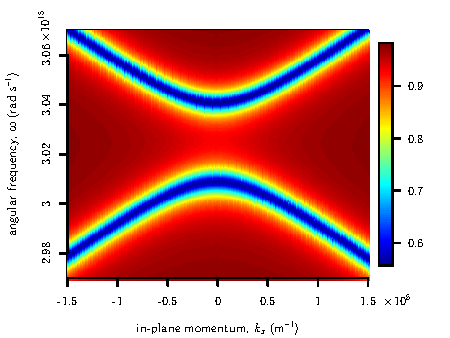
\includegraphics[]{figure-bandedgecoupling-band2}\label{fig:couplingbandedgesA}}
\subfigure[$\psi_2=90^\circ$]{% Created by tikzDevice version 0.6.2-92-0ad2792 on 2013-01-22 18:38:21
% !TEX encoding = UTF-8 Unicode
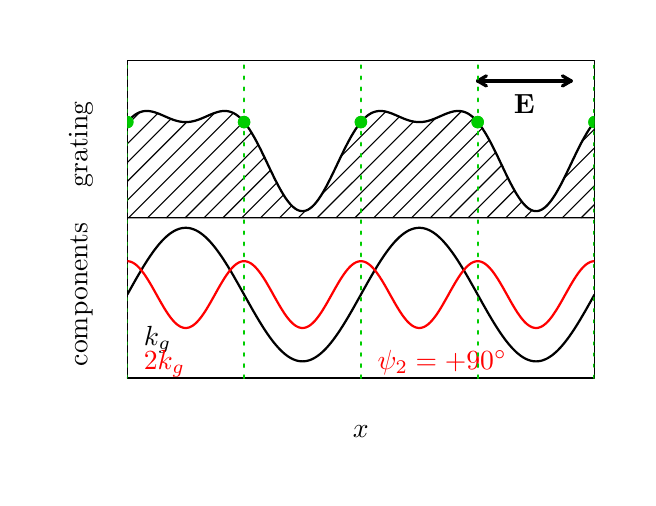
\begin{tikzpicture}[x=1pt,y=1pt]
\definecolor[named]{fillColor}{rgb}{1.00,1.00,1.00}
\path[use as bounding box,fill=fillColor,fill opacity=0.00] (0,0) rectangle (216.81,162.61);
\begin{scope}
\path[clip] ( 36.00, 36.00) rectangle (204.81,150.61);
\definecolor[named]{drawColor}{rgb}{0.00,0.00,0.00}

\path[draw=drawColor,line width= 0.8pt,line join=round,line cap=round] ( 36.00,128.49) --
	( 36.34,128.89) --
	( 36.68,129.26) --
	( 37.01,129.61) --
	( 37.35,129.95) --
	( 37.69,130.26) --
	( 38.03,130.55) --
	( 38.37,130.82) --
	( 38.71,131.07) --
	( 39.04,131.29) --
	( 39.38,131.50) --
	( 39.72,131.69) --
	( 40.06,131.85) --
	( 40.40,132.00) --
	( 40.74,132.13) --
	( 41.07,132.23) --
	( 41.41,132.32) --
	( 41.75,132.40) --
	( 42.09,132.45) --
	( 42.43,132.49) --
	( 42.77,132.51) --
	( 43.10,132.51) --
	( 43.44,132.50) --
	( 43.78,132.48) --
	( 44.12,132.44) --
	( 44.46,132.38) --
	( 44.80,132.32) --
	( 45.13,132.25) --
	( 45.47,132.16) --
	( 45.81,132.06) --
	( 46.15,131.96) --
	( 46.49,131.84) --
	( 46.83,131.72) --
	( 47.16,131.60) --
	( 47.50,131.46) --
	( 47.84,131.32) --
	( 48.18,131.18) --
	( 48.52,131.04) --
	( 48.86,130.89) --
	( 49.19,130.74) --
	( 49.53,130.59) --
	( 49.87,130.44) --
	( 50.21,130.30) --
	( 50.55,130.15) --
	( 50.89,130.00) --
	( 51.22,129.86) --
	( 51.56,129.73) --
	( 51.90,129.59) --
	( 52.24,129.47) --
	( 52.58,129.34) --
	( 52.91,129.23) --
	( 53.25,129.12) --
	( 53.59,129.02) --
	( 53.93,128.92) --
	( 54.27,128.84) --
	( 54.61,128.76) --
	( 54.94,128.69) --
	( 55.28,128.64) --
	( 55.62,128.59) --
	( 55.96,128.55) --
	( 56.30,128.52) --
	( 56.64,128.50) --
	( 56.97,128.49) --
	( 57.31,128.49) --
	( 57.65,128.50) --
	( 57.99,128.53) --
	( 58.33,128.56) --
	( 58.67,128.60) --
	( 59.00,128.65) --
	( 59.34,128.71) --
	( 59.68,128.78) --
	( 60.02,128.86) --
	( 60.36,128.95) --
	( 60.70,129.04) --
	( 61.03,129.15) --
	( 61.37,129.26) --
	( 61.71,129.37) --
	( 62.05,129.50) --
	( 62.39,129.63) --
	( 62.73,129.76) --
	( 63.06,129.90) --
	( 63.40,130.04) --
	( 63.74,130.18) --
	( 64.08,130.33) --
	( 64.42,130.48) --
	( 64.76,130.63) --
	( 65.09,130.78) --
	( 65.43,130.93) --
	( 65.77,131.07) --
	( 66.11,131.22) --
	( 66.45,131.36) --
	( 66.78,131.50) --
	( 67.12,131.63) --
	( 67.46,131.75) --
	( 67.80,131.87) --
	( 68.14,131.98) --
	( 68.48,132.09) --
	( 68.81,132.18) --
	( 69.15,132.27) --
	( 69.49,132.34) --
	( 69.83,132.40) --
	( 70.17,132.45) --
	( 70.51,132.48) --
	( 70.84,132.50) --
	( 71.18,132.51) --
	( 71.52,132.50) --
	( 71.86,132.48) --
	( 72.20,132.44) --
	( 72.54,132.38) --
	( 72.87,132.30) --
	( 73.21,132.21) --
	( 73.55,132.10) --
	( 73.89,131.96) --
	( 74.23,131.81) --
	( 74.57,131.64) --
	( 74.90,131.45) --
	( 75.24,131.24) --
	( 75.58,131.00) --
	( 75.92,130.75) --
	( 76.26,130.48) --
	( 76.60,130.18) --
	( 76.93,129.86) --
	( 77.27,129.53) --
	( 77.61,129.17) --
	( 77.95,128.79) --
	( 78.29,128.39) --
	( 78.63,127.97) --
	( 78.96,127.53) --
	( 79.30,127.07) --
	( 79.64,126.59) --
	( 79.98,126.09) --
	( 80.32,125.57) --
	( 80.66,125.04) --
	( 80.99,124.49) --
	( 81.33,123.92) --
	( 81.67,123.34) --
	( 82.01,122.74) --
	( 82.35,122.12) --
	( 82.68,121.50) --
	( 83.02,120.86) --
	( 83.36,120.21) --
	( 83.70,119.54) --
	( 84.04,118.87) --
	( 84.38,118.19) --
	( 84.71,117.50) --
	( 85.05,116.81) --
	( 85.39,116.10) --
	( 85.73,115.40) --
	( 86.07,114.69) --
	( 86.41,113.98) --
	( 86.74,113.26) --
	( 87.08,112.55) --
	( 87.42,111.84) --
	( 87.76,111.13) --
	( 88.10,110.43) --
	( 88.44,109.72) --
	( 88.77,109.03) --
	( 89.11,108.34) --
	( 89.45,107.66) --
	( 89.79,107.00) --
	( 90.13,106.34) --
	( 90.47,105.69) --
	( 90.80,105.06) --
	( 91.14,104.44) --
	( 91.48,103.84) --
	( 91.82,103.25) --
	( 92.16,102.68) --
	( 92.50,102.13) --
	( 92.83,101.60) --
	( 93.17,101.09) --
	( 93.51,100.60) --
	( 93.85,100.14) --
	( 94.19, 99.70) --
	( 94.53, 99.28) --
	( 94.86, 98.88) --
	( 95.20, 98.52) --
	( 95.54, 98.18) --
	( 95.88, 97.86) --
	( 96.22, 97.58) --
	( 96.56, 97.32) --
	( 96.89, 97.09) --
	( 97.23, 96.89) --
	( 97.57, 96.72) --
	( 97.91, 96.58) --
	( 98.25, 96.47) --
	( 98.58, 96.39) --
	( 98.92, 96.34) --
	( 99.26, 96.32) --
	( 99.60, 96.33) --
	( 99.94, 96.37) --
	(100.28, 96.45) --
	(100.61, 96.55) --
	(100.95, 96.68) --
	(101.29, 96.84) --
	(101.63, 97.04) --
	(101.97, 97.26) --
	(102.31, 97.51) --
	(102.64, 97.79) --
	(102.98, 98.10) --
	(103.32, 98.43) --
	(103.66, 98.79) --
	(104.00, 99.18) --
	(104.34, 99.59) --
	(104.67,100.02) --
	(105.01,100.48) --
	(105.35,100.97) --
	(105.69,101.47) --
	(106.03,102.00) --
	(106.37,102.54) --
	(106.70,103.11) --
	(107.04,103.69) --
	(107.38,104.29) --
	(107.72,104.90) --
	(108.06,105.53) --
	(108.40,106.17) --
	(108.73,106.83) --
	(109.07,107.50) --
	(109.41,108.17) --
	(109.75,108.86) --
	(110.09,109.55) --
	(110.43,110.25) --
	(110.76,110.95) --
	(111.10,111.66) --
	(111.44,112.37) --
	(111.78,113.09) --
	(112.12,113.80) --
	(112.46,114.51) --
	(112.79,115.22) --
	(113.13,115.93) --
	(113.47,116.63) --
	(113.81,117.33) --
	(114.15,118.02) --
	(114.48,118.70) --
	(114.82,119.38) --
	(115.16,120.04) --
	(115.50,120.70) --
	(115.84,121.34) --
	(116.18,121.97) --
	(116.51,122.58) --
	(116.85,123.19) --
	(117.19,123.78) --
	(117.53,124.35) --
	(117.87,124.90) --
	(118.21,125.44) --
	(118.54,125.96) --
	(118.88,126.47) --
	(119.22,126.95) --
	(119.56,127.41) --
	(119.90,127.86) --
	(120.24,128.29) --
	(120.57,128.69) --
	(120.91,129.07) --
	(121.25,129.44) --
	(121.59,129.78) --
	(121.93,130.10) --
	(122.27,130.40) --
	(122.60,130.68) --
	(122.94,130.94) --
	(123.28,131.18) --
	(123.62,131.40) --
	(123.96,131.60) --
	(124.30,131.77) --
	(124.63,131.93) --
	(124.97,132.07) --
	(125.31,132.18) --
	(125.65,132.28) --
	(125.99,132.36) --
	(126.33,132.42) --
	(126.66,132.47) --
	(127.00,132.50) --
	(127.34,132.51) --
	(127.68,132.51) --
	(128.02,132.49) --
	(128.35,132.46) --
	(128.69,132.41) --
	(129.03,132.35) --
	(129.37,132.28) --
	(129.71,132.20) --
	(130.05,132.11) --
	(130.38,132.01) --
	(130.72,131.90) --
	(131.06,131.78) --
	(131.40,131.66) --
	(131.74,131.53) --
	(132.08,131.39) --
	(132.41,131.25) --
	(132.75,131.11) --
	(133.09,130.96) --
	(133.43,130.82) --
	(133.77,130.67) --
	(134.11,130.52) --
	(134.44,130.37) --
	(134.78,130.22) --
	(135.12,130.08) --
	(135.46,129.93) --
	(135.80,129.79) --
	(136.14,129.66) --
	(136.47,129.53) --
	(136.81,129.40) --
	(137.15,129.28) --
	(137.49,129.17) --
	(137.83,129.07) --
	(138.17,128.97) --
	(138.50,128.88) --
	(138.84,128.80) --
	(139.18,128.73) --
	(139.52,128.66) --
	(139.86,128.61) --
	(140.20,128.57) --
	(140.53,128.53) --
	(140.87,128.51) --
	(141.21,128.49) --
	(141.55,128.49) --
	(141.89,128.50) --
	(142.23,128.51) --
	(142.56,128.54) --
	(142.90,128.58) --
	(143.24,128.62) --
	(143.58,128.68) --
	(143.92,128.74) --
	(144.25,128.82) --
	(144.59,128.90) --
	(144.93,128.99) --
	(145.27,129.09) --
	(145.61,129.20) --
	(145.95,129.31) --
	(146.28,129.43) --
	(146.62,129.56) --
	(146.96,129.69) --
	(147.30,129.83) --
	(147.64,129.97) --
	(147.98,130.11) --
	(148.31,130.26) --
	(148.65,130.41) --
	(148.99,130.56) --
	(149.33,130.70) --
	(149.67,130.85) --
	(150.01,131.00) --
	(150.34,131.15) --
	(150.68,131.29) --
	(151.02,131.43) --
	(151.36,131.56) --
	(151.70,131.69) --
	(152.04,131.81) --
	(152.37,131.93) --
	(152.71,132.04) --
	(153.05,132.14) --
	(153.39,132.22) --
	(153.73,132.30) --
	(154.07,132.37) --
	(154.40,132.42) --
	(154.74,132.47) --
	(155.08,132.50) --
	(155.42,132.51) --
	(155.76,132.51) --
	(156.10,132.49) --
	(156.43,132.46) --
	(156.77,132.41) --
	(157.11,132.34) --
	(157.45,132.26) --
	(157.79,132.16) --
	(158.13,132.03) --
	(158.46,131.89) --
	(158.80,131.73) --
	(159.14,131.55) --
	(159.48,131.35) --
	(159.82,131.12) --
	(160.15,130.88) --
	(160.49,130.62) --
	(160.83,130.33) --
	(161.17,130.03) --
	(161.51,129.70) --
	(161.85,129.35) --
	(162.18,128.98) --
	(162.52,128.59) --
	(162.86,128.18) --
	(163.20,127.75) --
	(163.54,127.30) --
	(163.88,126.83) --
	(164.21,126.34) --
	(164.55,125.83) --
	(164.89,125.31) --
	(165.23,124.77) --
	(165.57,124.21) --
	(165.91,123.63) --
	(166.24,123.04) --
	(166.58,122.43) --
	(166.92,121.81) --
	(167.26,121.18) --
	(167.60,120.53) --
	(167.94,119.88) --
	(168.27,119.21) --
	(168.61,118.53) --
	(168.95,117.85) --
	(169.29,117.15) --
	(169.63,116.46) --
	(169.97,115.75) --
	(170.30,115.04) --
	(170.64,114.33) --
	(170.98,113.62) --
	(171.32,112.91) --
	(171.66,112.20) --
	(172.00,111.49) --
	(172.33,110.78) --
	(172.67,110.07) --
	(173.01,109.38) --
	(173.35,108.69) --
	(173.69,108.00) --
	(174.03,107.33) --
	(174.36,106.66) --
	(174.70,106.01) --
	(175.04,105.37) --
	(175.38,104.75) --
	(175.72,104.14) --
	(176.05,103.54) --
	(176.39,102.96) --
	(176.73,102.40) --
	(177.07,101.86) --
	(177.41,101.34) --
	(177.75,100.84) --
	(178.08,100.37) --
	(178.42, 99.91) --
	(178.76, 99.48) --
	(179.10, 99.08) --
	(179.44, 98.70) --
	(179.78, 98.34) --
	(180.11, 98.02) --
	(180.45, 97.72) --
	(180.79, 97.44) --
	(181.13, 97.20) --
	(181.47, 96.99) --
	(181.81, 96.80) --
	(182.14, 96.65) --
	(182.48, 96.52) --
	(182.82, 96.42) --
	(183.16, 96.36) --
	(183.50, 96.33) --
	(183.84, 96.32) --
	(184.17, 96.35) --
	(184.51, 96.41) --
	(184.85, 96.49) --
	(185.19, 96.61) --
	(185.53, 96.76) --
	(185.87, 96.94) --
	(186.20, 97.14) --
	(186.54, 97.38) --
	(186.88, 97.65) --
	(187.22, 97.94) --
	(187.56, 98.26) --
	(187.90, 98.61) --
	(188.23, 98.98) --
	(188.57, 99.38) --
	(188.91, 99.80) --
	(189.25,100.25) --
	(189.59,100.72) --
	(189.92,101.22) --
	(190.26,101.73) --
	(190.60,102.27) --
	(190.94,102.82) --
	(191.28,103.40) --
	(191.62,103.99) --
	(191.95,104.59) --
	(192.29,105.22) --
	(192.63,105.85) --
	(192.97,106.50) --
	(193.31,107.16) --
	(193.65,107.83) --
	(193.98,108.51) --
	(194.32,109.20) --
	(194.66,109.90) --
	(195.00,110.60) --
	(195.34,111.31) --
	(195.68,112.02) --
	(196.01,112.73) --
	(196.35,113.44) --
	(196.69,114.16) --
	(197.03,114.87) --
	(197.37,115.58) --
	(197.71,116.28) --
	(198.04,116.98) --
	(198.38,117.67) --
	(198.72,118.36) --
	(199.06,119.04) --
	(199.40,119.71) --
	(199.74,120.37) --
	(200.07,121.02) --
	(200.41,121.65) --
	(200.75,122.28) --
	(201.09,122.89) --
	(201.43,123.48) --
	(201.77,124.06) --
	(202.10,124.63) --
	(202.44,125.17) --
	(202.78,125.70) --
	(203.12,126.22) --
	(203.46,126.71) --
	(203.80,127.18) --
	(204.13,127.64) --
	(204.47,128.08) --
	(204.81,128.49);
\end{scope}
\begin{scope}
\path[clip] (  0.00,  0.00) rectangle (216.81,162.61);
\definecolor[named]{drawColor}{rgb}{0.00,0.00,0.00}

\path[draw=drawColor,line width= 0.4pt,line join=round,line cap=round] ( 36.00, 36.00) --
	(204.81, 36.00) --
	(204.81,150.61) --
	( 36.00,150.61) --
	( 36.00, 36.00);
\end{scope}
\begin{scope}
\path[clip] (  0.00,  0.00) rectangle (216.81,162.61);
\definecolor[named]{drawColor}{rgb}{0.00,0.00,0.00}

\node[text=drawColor,rotate= 90.00,anchor=base,inner sep=0pt, outer sep=0pt, scale=  1.00] at ( 21.60,120.45) {grating};

\node[text=drawColor,rotate= 90.00,anchor=base,inner sep=0pt, outer sep=0pt, scale=  1.00] at ( 21.60, 66.16) {components};

\node[text=drawColor,anchor=base,inner sep=0pt, outer sep=0pt, scale=  1.00] at (120.41, 14.40) {$x$};
\end{scope}
\begin{scope}
\path[clip] ( 36.00, 36.00) rectangle (204.81,150.61);
\definecolor[named]{drawColor}{rgb}{0.00,0.00,0.00}

\node[text=drawColor,anchor=base west,inner sep=0pt, outer sep=0pt, scale=  1.00] at ( 42.00, 47.94) {$k_g$};
\definecolor[named]{drawColor}{rgb}{1.00,0.00,0.00}

\node[text=drawColor,anchor=base west,inner sep=0pt, outer sep=0pt, scale=  1.00] at ( 42.00, 39.25) {2$k_g$};

\node[text=drawColor,anchor=base west,inner sep=0pt, outer sep=0pt, scale=  1.00] at (126.41, 39.25) {$\psi_2=+90^\circ$};
\definecolor[named]{drawColor}{rgb}{0.00,0.00,0.00}

\path[draw=drawColor,line width= 1.2pt,line join=round,line cap=round] (162.61,143.37) -- (196.37,143.37);

\path[draw=drawColor,line width= 1.2pt,line join=round,line cap=round] (165.74,145.18) --
	(162.61,143.37) --
	(165.74,141.56);

\path[draw=drawColor,line width= 1.2pt,line join=round,line cap=round] (193.24,141.56) --
	(196.37,143.37) --
	(193.24,145.18);

\node[text=drawColor,anchor=base,inner sep=0pt, outer sep=0pt, scale=  1.00] at (179.49,131.63) {$\mathbf{E}$};

\path[draw=drawColor,line width= 0.4pt,line join=round,line cap=round] ( 36.00,127.48) -- ( 40.59,132.07);

\path[draw=drawColor,line width= 0.4pt,line join=round,line cap=round] ( 36.00,120.67) -- ( 46.99,131.66);

\path[draw=drawColor,line width= 0.4pt,line join=round,line cap=round] ( 36.00,113.86) -- ( 51.78,129.64);

\path[draw=drawColor,line width= 0.4pt,line join=round,line cap=round] ( 36.00,107.04) -- ( 57.46,128.50);

\path[draw=drawColor,line width= 0.4pt,line join=round,line cap=round] ( 36.00,100.23) -- ( 67.56,131.79);

\path[draw=drawColor,line width= 0.4pt,line join=round,line cap=round] ( 36.49, 93.91) -- ( 74.34,131.76);

\path[draw=drawColor,line width= 0.4pt,line join=round,line cap=round] ( 43.31, 93.91) -- ( 78.06,128.66);

\path[draw=drawColor,line width= 0.4pt,line join=round,line cap=round] ( 50.12, 93.91) -- ( 80.88,124.67);

\path[draw=drawColor,line width= 0.4pt,line join=round,line cap=round] ( 56.93, 93.91) -- ( 83.32,120.29);

\path[draw=drawColor,line width= 0.4pt,line join=round,line cap=round] ( 63.75, 93.91) -- ( 85.57,115.73);

\path[draw=drawColor,line width= 0.4pt,line join=round,line cap=round] ( 70.56, 93.91) -- ( 87.77,111.11);

\path[draw=drawColor,line width= 0.4pt,line join=round,line cap=round] ( 77.37, 93.91) -- ( 90.02,106.55);

\path[draw=drawColor,line width= 0.4pt,line join=round,line cap=round] ( 84.19, 93.91) -- ( 92.46,102.18);

\path[draw=drawColor,line width= 0.4pt,line join=round,line cap=round] ( 91.00, 93.91) -- ( 95.41, 98.31);

\path[draw=drawColor,line width= 0.4pt,line join=round,line cap=round] (113.23,116.14) -- (129.38,132.28);

\path[draw=drawColor,line width= 0.4pt,line join=round,line cap=round] ( 97.82, 93.91) -- (100.39, 96.48);

\path[draw=drawColor,line width= 0.4pt,line join=round,line cap=round] (106.23,102.32) -- (134.33,130.42);

\path[draw=drawColor,line width= 0.4pt,line join=round,line cap=round] (104.63, 93.91) -- (139.41,128.68);

\path[draw=drawColor,line width= 0.4pt,line join=round,line cap=round] (111.44, 93.91) -- (147.41,129.87);

\path[draw=drawColor,line width= 0.4pt,line join=round,line cap=round] (118.26, 93.91) -- (156.76,132.41);

\path[draw=drawColor,line width= 0.4pt,line join=round,line cap=round] (125.07, 93.91) -- (161.18,130.02);

\path[draw=drawColor,line width= 0.4pt,line join=round,line cap=round] (131.88, 93.91) -- (164.26,126.28);

\path[draw=drawColor,line width= 0.4pt,line join=round,line cap=round] (138.70, 93.91) -- (166.81,122.02);

\path[draw=drawColor,line width= 0.4pt,line join=round,line cap=round] (145.51, 93.91) -- (169.11,117.51);

\path[draw=drawColor,line width= 0.4pt,line join=round,line cap=round] (152.32, 93.91) -- (171.32,112.90);

\path[draw=drawColor,line width= 0.4pt,line join=round,line cap=round] (159.14, 93.91) -- (173.54,108.31);

\path[draw=drawColor,line width= 0.4pt,line join=round,line cap=round] (165.95, 93.91) -- (175.89,103.84);

\path[draw=drawColor,line width= 0.4pt,line join=round,line cap=round] (172.77, 93.91) -- (178.58, 99.72);

\path[draw=drawColor,line width= 0.4pt,line join=round,line cap=round] (200.30,121.44) -- (205.18,126.32);

\path[draw=drawColor,line width= 0.4pt,line join=round,line cap=round] (179.58, 93.91) -- (182.27, 96.60);

\path[draw=drawColor,line width= 0.4pt,line join=round,line cap=round] (193.78,108.11) -- (206.16,120.49);

\path[draw=drawColor,line width= 0.4pt,line join=round,line cap=round] (186.39, 93.91) -- (207.14,114.65);

\path[draw=drawColor,line width= 0.4pt,line join=round,line cap=round] (193.21, 93.91) -- (208.12,108.82);

\path[draw=drawColor,line width= 0.4pt,line join=round,line cap=round] (200.02, 93.91) -- (209.11,102.99);

\path[draw=drawColor,line width= 0.4pt,line join=round,line cap=round] (206.83, 93.91) -- (210.09, 97.16);

\path[draw=drawColor,line width= 0.4pt,line join=round,line cap=round] ( 36.00,128.49) --
	( 36.34,128.89) --
	( 36.68,129.26) --
	( 37.01,129.61) --
	( 37.35,129.95) --
	( 37.69,130.26) --
	( 38.03,130.55) --
	( 38.37,130.82) --
	( 38.71,131.07) --
	( 39.04,131.29) --
	( 39.38,131.50) --
	( 39.72,131.69) --
	( 40.06,131.85) --
	( 40.40,132.00) --
	( 40.74,132.13) --
	( 41.07,132.23) --
	( 41.41,132.32) --
	( 41.75,132.40) --
	( 42.09,132.45) --
	( 42.43,132.49) --
	( 42.77,132.51) --
	( 43.10,132.51) --
	( 43.44,132.50) --
	( 43.78,132.48) --
	( 44.12,132.44) --
	( 44.46,132.38) --
	( 44.80,132.32) --
	( 45.13,132.25) --
	( 45.47,132.16) --
	( 45.81,132.06) --
	( 46.15,131.96) --
	( 46.49,131.84) --
	( 46.83,131.72) --
	( 47.16,131.60) --
	( 47.50,131.46) --
	( 47.84,131.32) --
	( 48.18,131.18) --
	( 48.52,131.04) --
	( 48.86,130.89) --
	( 49.19,130.74) --
	( 49.53,130.59) --
	( 49.87,130.44) --
	( 50.21,130.30) --
	( 50.55,130.15) --
	( 50.89,130.00) --
	( 51.22,129.86) --
	( 51.56,129.73) --
	( 51.90,129.59) --
	( 52.24,129.47) --
	( 52.58,129.34) --
	( 52.91,129.23) --
	( 53.25,129.12) --
	( 53.59,129.02) --
	( 53.93,128.92) --
	( 54.27,128.84) --
	( 54.61,128.76) --
	( 54.94,128.69) --
	( 55.28,128.64) --
	( 55.62,128.59) --
	( 55.96,128.55) --
	( 56.30,128.52) --
	( 56.64,128.50) --
	( 56.97,128.49) --
	( 57.31,128.49) --
	( 57.65,128.50) --
	( 57.99,128.53) --
	( 58.33,128.56) --
	( 58.67,128.60) --
	( 59.00,128.65) --
	( 59.34,128.71) --
	( 59.68,128.78) --
	( 60.02,128.86) --
	( 60.36,128.95) --
	( 60.70,129.04) --
	( 61.03,129.15) --
	( 61.37,129.26) --
	( 61.71,129.37) --
	( 62.05,129.50) --
	( 62.39,129.63) --
	( 62.73,129.76) --
	( 63.06,129.90) --
	( 63.40,130.04) --
	( 63.74,130.18) --
	( 64.08,130.33) --
	( 64.42,130.48) --
	( 64.76,130.63) --
	( 65.09,130.78) --
	( 65.43,130.93) --
	( 65.77,131.07) --
	( 66.11,131.22) --
	( 66.45,131.36) --
	( 66.78,131.50) --
	( 67.12,131.63) --
	( 67.46,131.75) --
	( 67.80,131.87) --
	( 68.14,131.98) --
	( 68.48,132.09) --
	( 68.81,132.18) --
	( 69.15,132.27) --
	( 69.49,132.34) --
	( 69.83,132.40) --
	( 70.17,132.45) --
	( 70.51,132.48) --
	( 70.84,132.50) --
	( 71.18,132.51) --
	( 71.52,132.50) --
	( 71.86,132.48) --
	( 72.20,132.44) --
	( 72.54,132.38) --
	( 72.87,132.30) --
	( 73.21,132.21) --
	( 73.55,132.10) --
	( 73.89,131.96) --
	( 74.23,131.81) --
	( 74.57,131.64) --
	( 74.90,131.45) --
	( 75.24,131.24) --
	( 75.58,131.00) --
	( 75.92,130.75) --
	( 76.26,130.48) --
	( 76.60,130.18) --
	( 76.93,129.86) --
	( 77.27,129.53) --
	( 77.61,129.17) --
	( 77.95,128.79) --
	( 78.29,128.39) --
	( 78.63,127.97) --
	( 78.96,127.53) --
	( 79.30,127.07) --
	( 79.64,126.59) --
	( 79.98,126.09) --
	( 80.32,125.57) --
	( 80.66,125.04) --
	( 80.99,124.49) --
	( 81.33,123.92) --
	( 81.67,123.34) --
	( 82.01,122.74) --
	( 82.35,122.12) --
	( 82.68,121.50) --
	( 83.02,120.86) --
	( 83.36,120.21) --
	( 83.70,119.54) --
	( 84.04,118.87) --
	( 84.38,118.19) --
	( 84.71,117.50) --
	( 85.05,116.81) --
	( 85.39,116.10) --
	( 85.73,115.40) --
	( 86.07,114.69) --
	( 86.41,113.98) --
	( 86.74,113.26) --
	( 87.08,112.55) --
	( 87.42,111.84) --
	( 87.76,111.13) --
	( 88.10,110.43) --
	( 88.44,109.72) --
	( 88.77,109.03) --
	( 89.11,108.34) --
	( 89.45,107.66) --
	( 89.79,107.00) --
	( 90.13,106.34) --
	( 90.47,105.69) --
	( 90.80,105.06) --
	( 91.14,104.44) --
	( 91.48,103.84) --
	( 91.82,103.25) --
	( 92.16,102.68) --
	( 92.50,102.13) --
	( 92.83,101.60) --
	( 93.17,101.09) --
	( 93.51,100.60) --
	( 93.85,100.14) --
	( 94.19, 99.70) --
	( 94.53, 99.28) --
	( 94.86, 98.88) --
	( 95.20, 98.52) --
	( 95.54, 98.18) --
	( 95.88, 97.86) --
	( 96.22, 97.58) --
	( 96.56, 97.32) --
	( 96.89, 97.09) --
	( 97.23, 96.89) --
	( 97.57, 96.72) --
	( 97.91, 96.58) --
	( 98.25, 96.47) --
	( 98.58, 96.39) --
	( 98.92, 96.34) --
	( 99.26, 96.32) --
	( 99.60, 96.33) --
	( 99.94, 96.37) --
	(100.28, 96.45) --
	(100.61, 96.55) --
	(100.95, 96.68) --
	(101.29, 96.84) --
	(101.63, 97.04) --
	(101.97, 97.26) --
	(102.31, 97.51) --
	(102.64, 97.79) --
	(102.98, 98.10) --
	(103.32, 98.43) --
	(103.66, 98.79) --
	(104.00, 99.18) --
	(104.34, 99.59) --
	(104.67,100.02) --
	(105.01,100.48) --
	(105.35,100.97) --
	(105.69,101.47) --
	(106.03,102.00) --
	(106.37,102.54) --
	(106.70,103.11) --
	(107.04,103.69) --
	(107.38,104.29) --
	(107.72,104.90) --
	(108.06,105.53) --
	(108.40,106.17) --
	(108.73,106.83) --
	(109.07,107.50) --
	(109.41,108.17) --
	(109.75,108.86) --
	(110.09,109.55) --
	(110.43,110.25) --
	(110.76,110.95) --
	(111.10,111.66) --
	(111.44,112.37) --
	(111.78,113.09) --
	(112.12,113.80) --
	(112.46,114.51) --
	(112.79,115.22) --
	(113.13,115.93) --
	(113.47,116.63) --
	(113.81,117.33) --
	(114.15,118.02) --
	(114.48,118.70) --
	(114.82,119.38) --
	(115.16,120.04) --
	(115.50,120.70) --
	(115.84,121.34) --
	(116.18,121.97) --
	(116.51,122.58) --
	(116.85,123.19) --
	(117.19,123.78) --
	(117.53,124.35) --
	(117.87,124.90) --
	(118.21,125.44) --
	(118.54,125.96) --
	(118.88,126.47) --
	(119.22,126.95) --
	(119.56,127.41) --
	(119.90,127.86) --
	(120.24,128.29) --
	(120.57,128.69) --
	(120.91,129.07) --
	(121.25,129.44) --
	(121.59,129.78) --
	(121.93,130.10) --
	(122.27,130.40) --
	(122.60,130.68) --
	(122.94,130.94) --
	(123.28,131.18) --
	(123.62,131.40) --
	(123.96,131.60) --
	(124.30,131.77) --
	(124.63,131.93) --
	(124.97,132.07) --
	(125.31,132.18) --
	(125.65,132.28) --
	(125.99,132.36) --
	(126.33,132.42) --
	(126.66,132.47) --
	(127.00,132.50) --
	(127.34,132.51) --
	(127.68,132.51) --
	(128.02,132.49) --
	(128.35,132.46) --
	(128.69,132.41) --
	(129.03,132.35) --
	(129.37,132.28) --
	(129.71,132.20) --
	(130.05,132.11) --
	(130.38,132.01) --
	(130.72,131.90) --
	(131.06,131.78) --
	(131.40,131.66) --
	(131.74,131.53) --
	(132.08,131.39) --
	(132.41,131.25) --
	(132.75,131.11) --
	(133.09,130.96) --
	(133.43,130.82) --
	(133.77,130.67) --
	(134.11,130.52) --
	(134.44,130.37) --
	(134.78,130.22) --
	(135.12,130.08) --
	(135.46,129.93) --
	(135.80,129.79) --
	(136.14,129.66) --
	(136.47,129.53) --
	(136.81,129.40) --
	(137.15,129.28) --
	(137.49,129.17) --
	(137.83,129.07) --
	(138.17,128.97) --
	(138.50,128.88) --
	(138.84,128.80) --
	(139.18,128.73) --
	(139.52,128.66) --
	(139.86,128.61) --
	(140.20,128.57) --
	(140.53,128.53) --
	(140.87,128.51) --
	(141.21,128.49) --
	(141.55,128.49) --
	(141.89,128.50) --
	(142.23,128.51) --
	(142.56,128.54) --
	(142.90,128.58) --
	(143.24,128.62) --
	(143.58,128.68) --
	(143.92,128.74) --
	(144.25,128.82) --
	(144.59,128.90) --
	(144.93,128.99) --
	(145.27,129.09) --
	(145.61,129.20) --
	(145.95,129.31) --
	(146.28,129.43) --
	(146.62,129.56) --
	(146.96,129.69) --
	(147.30,129.83) --
	(147.64,129.97) --
	(147.98,130.11) --
	(148.31,130.26) --
	(148.65,130.41) --
	(148.99,130.56) --
	(149.33,130.70) --
	(149.67,130.85) --
	(150.01,131.00) --
	(150.34,131.15) --
	(150.68,131.29) --
	(151.02,131.43) --
	(151.36,131.56) --
	(151.70,131.69) --
	(152.04,131.81) --
	(152.37,131.93) --
	(152.71,132.04) --
	(153.05,132.14) --
	(153.39,132.22) --
	(153.73,132.30) --
	(154.07,132.37) --
	(154.40,132.42) --
	(154.74,132.47) --
	(155.08,132.50) --
	(155.42,132.51) --
	(155.76,132.51) --
	(156.10,132.49) --
	(156.43,132.46) --
	(156.77,132.41) --
	(157.11,132.34) --
	(157.45,132.26) --
	(157.79,132.16) --
	(158.13,132.03) --
	(158.46,131.89) --
	(158.80,131.73) --
	(159.14,131.55) --
	(159.48,131.35) --
	(159.82,131.12) --
	(160.15,130.88) --
	(160.49,130.62) --
	(160.83,130.33) --
	(161.17,130.03) --
	(161.51,129.70) --
	(161.85,129.35) --
	(162.18,128.98) --
	(162.52,128.59) --
	(162.86,128.18) --
	(163.20,127.75) --
	(163.54,127.30) --
	(163.88,126.83) --
	(164.21,126.34) --
	(164.55,125.83) --
	(164.89,125.31) --
	(165.23,124.77) --
	(165.57,124.21) --
	(165.91,123.63) --
	(166.24,123.04) --
	(166.58,122.43) --
	(166.92,121.81) --
	(167.26,121.18) --
	(167.60,120.53) --
	(167.94,119.88) --
	(168.27,119.21) --
	(168.61,118.53) --
	(168.95,117.85) --
	(169.29,117.15) --
	(169.63,116.46) --
	(169.97,115.75) --
	(170.30,115.04) --
	(170.64,114.33) --
	(170.98,113.62) --
	(171.32,112.91) --
	(171.66,112.20) --
	(172.00,111.49) --
	(172.33,110.78) --
	(172.67,110.07) --
	(173.01,109.38) --
	(173.35,108.69) --
	(173.69,108.00) --
	(174.03,107.33) --
	(174.36,106.66) --
	(174.70,106.01) --
	(175.04,105.37) --
	(175.38,104.75) --
	(175.72,104.14) --
	(176.05,103.54) --
	(176.39,102.96) --
	(176.73,102.40) --
	(177.07,101.86) --
	(177.41,101.34) --
	(177.75,100.84) --
	(178.08,100.37) --
	(178.42, 99.91) --
	(178.76, 99.48) --
	(179.10, 99.08) --
	(179.44, 98.70) --
	(179.78, 98.34) --
	(180.11, 98.02) --
	(180.45, 97.72) --
	(180.79, 97.44) --
	(181.13, 97.20) --
	(181.47, 96.99) --
	(181.81, 96.80) --
	(182.14, 96.65) --
	(182.48, 96.52) --
	(182.82, 96.42) --
	(183.16, 96.36) --
	(183.50, 96.33) --
	(183.84, 96.32) --
	(184.17, 96.35) --
	(184.51, 96.41) --
	(184.85, 96.49) --
	(185.19, 96.61) --
	(185.53, 96.76) --
	(185.87, 96.94) --
	(186.20, 97.14) --
	(186.54, 97.38) --
	(186.88, 97.65) --
	(187.22, 97.94) --
	(187.56, 98.26) --
	(187.90, 98.61) --
	(188.23, 98.98) --
	(188.57, 99.38) --
	(188.91, 99.80) --
	(189.25,100.25) --
	(189.59,100.72) --
	(189.92,101.22) --
	(190.26,101.73) --
	(190.60,102.27) --
	(190.94,102.82) --
	(191.28,103.40) --
	(191.62,103.99) --
	(191.95,104.59) --
	(192.29,105.22) --
	(192.63,105.85) --
	(192.97,106.50) --
	(193.31,107.16) --
	(193.65,107.83) --
	(193.98,108.51) --
	(194.32,109.20) --
	(194.66,109.90) --
	(195.00,110.60) --
	(195.34,111.31) --
	(195.68,112.02) --
	(196.01,112.73) --
	(196.35,113.44) --
	(196.69,114.16) --
	(197.03,114.87) --
	(197.37,115.58) --
	(197.71,116.28) --
	(198.04,116.98) --
	(198.38,117.67) --
	(198.72,118.36) --
	(199.06,119.04) --
	(199.40,119.71) --
	(199.74,120.37) --
	(200.07,121.02) --
	(200.41,121.65) --
	(200.75,122.28) --
	(201.09,122.89) --
	(201.43,123.48) --
	(201.77,124.06) --
	(202.10,124.63) --
	(202.44,125.17) --
	(202.78,125.70) --
	(203.12,126.22) --
	(203.46,126.71) --
	(203.80,127.18) --
	(204.13,127.64) --
	(204.47,128.08) --
	(204.81,128.49) --
	(210.64, 93.91) --
	( 36.00, 93.91) --
	( 36.00,128.49);

\path[draw=drawColor,line width= 0.8pt,line join=round,line cap=round] ( 36.00, 66.16) --
	( 36.34, 66.77) --
	( 36.68, 67.37) --
	( 37.01, 67.98) --
	( 37.35, 68.59) --
	( 37.69, 69.19) --
	( 38.03, 69.79) --
	( 38.37, 70.39) --
	( 38.71, 70.99) --
	( 39.04, 71.58) --
	( 39.38, 72.17) --
	( 39.72, 72.76) --
	( 40.06, 73.34) --
	( 40.40, 73.92) --
	( 40.74, 74.49) --
	( 41.07, 75.06) --
	( 41.41, 75.62) --
	( 41.75, 76.18) --
	( 42.09, 76.73) --
	( 42.43, 77.27) --
	( 42.77, 77.80) --
	( 43.10, 78.33) --
	( 43.44, 78.85) --
	( 43.78, 79.37) --
	( 44.12, 79.87) --
	( 44.46, 80.37) --
	( 44.80, 80.85) --
	( 45.13, 81.33) --
	( 45.47, 81.80) --
	( 45.81, 82.26) --
	( 46.15, 82.70) --
	( 46.49, 83.14) --
	( 46.83, 83.57) --
	( 47.16, 83.98) --
	( 47.50, 84.39) --
	( 47.84, 84.78) --
	( 48.18, 85.16) --
	( 48.52, 85.53) --
	( 48.86, 85.88) --
	( 49.19, 86.23) --
	( 49.53, 86.56) --
	( 49.87, 86.88) --
	( 50.21, 87.18) --
	( 50.55, 87.47) --
	( 50.89, 87.75) --
	( 51.22, 88.01) --
	( 51.56, 88.27) --
	( 51.90, 88.50) --
	( 52.24, 88.72) --
	( 52.58, 88.93) --
	( 52.91, 89.13) --
	( 53.25, 89.30) --
	( 53.59, 89.47) --
	( 53.93, 89.62) --
	( 54.27, 89.75) --
	( 54.61, 89.87) --
	( 54.94, 89.98) --
	( 55.28, 90.07) --
	( 55.62, 90.14) --
	( 55.96, 90.20) --
	( 56.30, 90.24) --
	( 56.64, 90.27) --
	( 56.97, 90.29) --
	( 57.31, 90.28) --
	( 57.65, 90.27) --
	( 57.99, 90.24) --
	( 58.33, 90.19) --
	( 58.67, 90.12) --
	( 59.00, 90.05) --
	( 59.34, 89.95) --
	( 59.68, 89.84) --
	( 60.02, 89.72) --
	( 60.36, 89.58) --
	( 60.70, 89.43) --
	( 61.03, 89.26) --
	( 61.37, 89.08) --
	( 61.71, 88.88) --
	( 62.05, 88.67) --
	( 62.39, 88.44) --
	( 62.73, 88.20) --
	( 63.06, 87.95) --
	( 63.40, 87.68) --
	( 63.74, 87.40) --
	( 64.08, 87.11) --
	( 64.42, 86.80) --
	( 64.76, 86.48) --
	( 65.09, 86.14) --
	( 65.43, 85.80) --
	( 65.77, 85.44) --
	( 66.11, 85.06) --
	( 66.45, 84.68) --
	( 66.78, 84.29) --
	( 67.12, 83.88) --
	( 67.46, 83.46) --
	( 67.80, 83.03) --
	( 68.14, 82.59) --
	( 68.48, 82.14) --
	( 68.81, 81.68) --
	( 69.15, 81.21) --
	( 69.49, 80.73) --
	( 69.83, 80.24) --
	( 70.17, 79.75) --
	( 70.51, 79.24) --
	( 70.84, 78.72) --
	( 71.18, 78.20) --
	( 71.52, 77.67) --
	( 71.86, 77.13) --
	( 72.20, 76.59) --
	( 72.54, 76.04) --
	( 72.87, 75.48) --
	( 73.21, 74.92) --
	( 73.55, 74.35) --
	( 73.89, 73.77) --
	( 74.23, 73.20) --
	( 74.57, 72.61) --
	( 74.90, 72.02) --
	( 75.24, 71.43) --
	( 75.58, 70.84) --
	( 75.92, 70.24) --
	( 76.26, 69.64) --
	( 76.60, 69.04) --
	( 76.93, 68.44) --
	( 77.27, 67.83) --
	( 77.61, 67.22) --
	( 77.95, 66.62) --
	( 78.29, 66.01) --
	( 78.63, 65.40) --
	( 78.96, 64.79) --
	( 79.30, 64.19) --
	( 79.64, 63.58) --
	( 79.98, 62.98) --
	( 80.32, 62.38) --
	( 80.66, 61.78) --
	( 80.99, 61.18) --
	( 81.33, 60.59) --
	( 81.67, 60.00) --
	( 82.01, 59.42) --
	( 82.35, 58.83) --
	( 82.68, 58.26) --
	( 83.02, 57.69) --
	( 83.36, 57.12) --
	( 83.70, 56.56) --
	( 84.04, 56.01) --
	( 84.38, 55.46) --
	( 84.71, 54.92) --
	( 85.05, 54.38) --
	( 85.39, 53.86) --
	( 85.73, 53.34) --
	( 86.07, 52.83) --
	( 86.41, 52.32) --
	( 86.74, 51.83) --
	( 87.08, 51.35) --
	( 87.42, 50.87) --
	( 87.76, 50.41) --
	( 88.10, 49.95) --
	( 88.44, 49.51) --
	( 88.77, 49.07) --
	( 89.11, 48.65) --
	( 89.45, 48.24) --
	( 89.79, 47.84) --
	( 90.13, 47.45) --
	( 90.47, 47.07) --
	( 90.80, 46.70) --
	( 91.14, 46.35) --
	( 91.48, 46.01) --
	( 91.82, 45.68) --
	( 92.16, 45.37) --
	( 92.50, 45.06) --
	( 92.83, 44.78) --
	( 93.17, 44.50) --
	( 93.51, 44.24) --
	( 93.85, 43.99) --
	( 94.19, 43.76) --
	( 94.53, 43.54) --
	( 94.86, 43.34) --
	( 95.20, 43.15) --
	( 95.54, 42.97) --
	( 95.88, 42.81) --
	( 96.22, 42.67) --
	( 96.56, 42.54) --
	( 96.89, 42.42) --
	( 97.23, 42.32) --
	( 97.57, 42.23) --
	( 97.91, 42.16) --
	( 98.25, 42.11) --
	( 98.58, 42.07) --
	( 98.92, 42.04) --
	( 99.26, 42.03) --
	( 99.60, 42.04) --
	( 99.94, 42.06) --
	(100.28, 42.10) --
	(100.61, 42.15) --
	(100.95, 42.21) --
	(101.29, 42.30) --
	(101.63, 42.39) --
	(101.97, 42.50) --
	(102.31, 42.63) --
	(102.64, 42.77) --
	(102.98, 42.93) --
	(103.32, 43.10) --
	(103.66, 43.29) --
	(104.00, 43.49) --
	(104.34, 43.71) --
	(104.67, 43.93) --
	(105.01, 44.18) --
	(105.35, 44.44) --
	(105.69, 44.71) --
	(106.03, 44.99) --
	(106.37, 45.29) --
	(106.70, 45.60) --
	(107.04, 45.93) --
	(107.38, 46.26) --
	(107.72, 46.61) --
	(108.06, 46.98) --
	(108.40, 47.35) --
	(108.73, 47.74) --
	(109.07, 48.13) --
	(109.41, 48.54) --
	(109.75, 48.97) --
	(110.09, 49.40) --
	(110.43, 49.84) --
	(110.76, 50.29) --
	(111.10, 50.75) --
	(111.44, 51.23) --
	(111.78, 51.71) --
	(112.12, 52.20) --
	(112.46, 52.70) --
	(112.79, 53.21) --
	(113.13, 53.73) --
	(113.47, 54.25) --
	(113.81, 54.78) --
	(114.15, 55.32) --
	(114.48, 55.87) --
	(114.82, 56.42) --
	(115.16, 56.98) --
	(115.50, 57.54) --
	(115.84, 58.11) --
	(116.18, 58.69) --
	(116.51, 59.27) --
	(116.85, 59.85) --
	(117.19, 60.44) --
	(117.53, 61.03) --
	(117.87, 61.63) --
	(118.21, 62.23) --
	(118.54, 62.83) --
	(118.88, 63.43) --
	(119.22, 64.04) --
	(119.56, 64.64) --
	(119.90, 65.25) --
	(120.24, 65.86) --
	(120.57, 66.46) --
	(120.91, 67.07) --
	(121.25, 67.68) --
	(121.59, 68.28) --
	(121.93, 68.89) --
	(122.27, 69.49) --
	(122.60, 70.09) --
	(122.94, 70.69) --
	(123.28, 71.29) --
	(123.62, 71.88) --
	(123.96, 72.47) --
	(124.30, 73.05) --
	(124.63, 73.63) --
	(124.97, 74.21) --
	(125.31, 74.78) --
	(125.65, 75.34) --
	(125.99, 75.90) --
	(126.33, 76.45) --
	(126.66, 77.00) --
	(127.00, 77.54) --
	(127.34, 78.07) --
	(127.68, 78.59) --
	(128.02, 79.11) --
	(128.35, 79.62) --
	(128.69, 80.12) --
	(129.03, 80.61) --
	(129.37, 81.09) --
	(129.71, 81.57) --
	(130.05, 82.03) --
	(130.38, 82.48) --
	(130.72, 82.92) --
	(131.06, 83.35) --
	(131.40, 83.78) --
	(131.74, 84.18) --
	(132.08, 84.58) --
	(132.41, 84.97) --
	(132.75, 85.34) --
	(133.09, 85.71) --
	(133.43, 86.06) --
	(133.77, 86.39) --
	(134.11, 86.72) --
	(134.44, 87.03) --
	(134.78, 87.33) --
	(135.12, 87.61) --
	(135.46, 87.88) --
	(135.80, 88.14) --
	(136.14, 88.39) --
	(136.47, 88.61) --
	(136.81, 88.83) --
	(137.15, 89.03) --
	(137.49, 89.22) --
	(137.83, 89.39) --
	(138.17, 89.55) --
	(138.50, 89.69) --
	(138.84, 89.81) --
	(139.18, 89.93) --
	(139.52, 90.02) --
	(139.86, 90.11) --
	(140.20, 90.17) --
	(140.53, 90.22) --
	(140.87, 90.26) --
	(141.21, 90.28) --
	(141.55, 90.29) --
	(141.89, 90.28) --
	(142.23, 90.25) --
	(142.56, 90.21) --
	(142.90, 90.16) --
	(143.24, 90.09) --
	(143.58, 90.00) --
	(143.92, 89.90) --
	(144.25, 89.78) --
	(144.59, 89.65) --
	(144.93, 89.51) --
	(145.27, 89.35) --
	(145.61, 89.17) --
	(145.95, 88.98) --
	(146.28, 88.78) --
	(146.62, 88.56) --
	(146.96, 88.33) --
	(147.30, 88.08) --
	(147.64, 87.82) --
	(147.98, 87.54) --
	(148.31, 87.25) --
	(148.65, 86.95) --
	(148.99, 86.64) --
	(149.33, 86.31) --
	(149.67, 85.97) --
	(150.01, 85.62) --
	(150.34, 85.25) --
	(150.68, 84.87) --
	(151.02, 84.48) --
	(151.36, 84.08) --
	(151.70, 83.67) --
	(152.04, 83.25) --
	(152.37, 82.81) --
	(152.71, 82.37) --
	(153.05, 81.91) --
	(153.39, 81.45) --
	(153.73, 80.97) --
	(154.07, 80.49) --
	(154.40, 80.00) --
	(154.74, 79.49) --
	(155.08, 78.98) --
	(155.42, 78.46) --
	(155.76, 77.94) --
	(156.10, 77.40) --
	(156.43, 76.86) --
	(156.77, 76.31) --
	(157.11, 75.76) --
	(157.45, 75.20) --
	(157.79, 74.63) --
	(158.13, 74.06) --
	(158.46, 73.49) --
	(158.80, 72.90) --
	(159.14, 72.32) --
	(159.48, 71.73) --
	(159.82, 71.14) --
	(160.15, 70.54) --
	(160.49, 69.94) --
	(160.83, 69.34) --
	(161.17, 68.74) --
	(161.51, 68.13) --
	(161.85, 67.53) --
	(162.18, 66.92) --
	(162.52, 66.31) --
	(162.86, 65.70) --
	(163.20, 65.10) --
	(163.54, 64.49) --
	(163.88, 63.88) --
	(164.21, 63.28) --
	(164.55, 62.68) --
	(164.89, 62.08) --
	(165.23, 61.48) --
	(165.57, 60.89) --
	(165.91, 60.29) --
	(166.24, 59.71) --
	(166.58, 59.12) --
	(166.92, 58.55) --
	(167.26, 57.97) --
	(167.60, 57.40) --
	(167.94, 56.84) --
	(168.27, 56.28) --
	(168.61, 55.73) --
	(168.95, 55.19) --
	(169.29, 54.65) --
	(169.63, 54.12) --
	(169.97, 53.60) --
	(170.30, 53.08) --
	(170.64, 52.57) --
	(170.98, 52.08) --
	(171.32, 51.59) --
	(171.66, 51.11) --
	(172.00, 50.64) --
	(172.33, 50.18) --
	(172.67, 49.73) --
	(173.01, 49.29) --
	(173.35, 48.86) --
	(173.69, 48.44) --
	(174.03, 48.03) --
	(174.36, 47.64) --
	(174.70, 47.26) --
	(175.04, 46.88) --
	(175.38, 46.52) --
	(175.72, 46.18) --
	(176.05, 45.84) --
	(176.39, 45.52) --
	(176.73, 45.21) --
	(177.07, 44.92) --
	(177.41, 44.64) --
	(177.75, 44.37) --
	(178.08, 44.12) --
	(178.42, 43.88) --
	(178.76, 43.65) --
	(179.10, 43.44) --
	(179.44, 43.24) --
	(179.78, 43.06) --
	(180.11, 42.89) --
	(180.45, 42.74) --
	(180.79, 42.60) --
	(181.13, 42.48) --
	(181.47, 42.37) --
	(181.81, 42.27) --
	(182.14, 42.20) --
	(182.48, 42.13) --
	(182.82, 42.08) --
	(183.16, 42.05) --
	(183.50, 42.03) --
	(183.84, 42.03) --
	(184.17, 42.05) --
	(184.51, 42.08) --
	(184.85, 42.12) --
	(185.19, 42.18) --
	(185.53, 42.25) --
	(185.87, 42.34) --
	(186.20, 42.45) --
	(186.54, 42.57) --
	(186.88, 42.70) --
	(187.22, 42.85) --
	(187.56, 43.02) --
	(187.90, 43.19) --
	(188.23, 43.39) --
	(188.57, 43.60) --
	(188.91, 43.82) --
	(189.25, 44.05) --
	(189.59, 44.31) --
	(189.92, 44.57) --
	(190.26, 44.85) --
	(190.60, 45.14) --
	(190.94, 45.44) --
	(191.28, 45.76) --
	(191.62, 46.09) --
	(191.95, 46.44) --
	(192.29, 46.79) --
	(192.63, 47.16) --
	(192.97, 47.54) --
	(193.31, 47.93) --
	(193.65, 48.34) --
	(193.98, 48.75) --
	(194.32, 49.18) --
	(194.66, 49.62) --
	(195.00, 50.06) --
	(195.34, 50.52) --
	(195.68, 50.99) --
	(196.01, 51.47) --
	(196.35, 51.95) --
	(196.69, 52.45) --
	(197.03, 52.95) --
	(197.37, 53.47) --
	(197.71, 53.99) --
	(198.04, 54.51) --
	(198.38, 55.05) --
	(198.72, 55.59) --
	(199.06, 56.14) --
	(199.40, 56.70) --
	(199.74, 57.26) --
	(200.07, 57.83) --
	(200.41, 58.40) --
	(200.75, 58.98) --
	(201.09, 59.56) --
	(201.43, 60.15) --
	(201.77, 60.74) --
	(202.10, 61.33) --
	(202.44, 61.93) --
	(202.78, 62.53) --
	(203.12, 63.13) --
	(203.46, 63.73) --
	(203.80, 64.34) --
	(204.13, 64.95) --
	(204.47, 65.55) --
	(204.81, 66.16);
\definecolor[named]{drawColor}{rgb}{1.00,0.00,0.00}

\path[draw=drawColor,line width= 0.8pt,line join=round,line cap=round] ( 36.00, 78.22) --
	( 36.34, 78.21) --
	( 36.68, 78.16) --
	( 37.01, 78.09) --
	( 37.35, 77.98) --
	( 37.69, 77.84) --
	( 38.03, 77.68) --
	( 38.37, 77.48) --
	( 38.71, 77.26) --
	( 39.04, 77.01) --
	( 39.38, 76.73) --
	( 39.72, 76.42) --
	( 40.06, 76.09) --
	( 40.40, 75.73) --
	( 40.74, 75.35) --
	( 41.07, 74.94) --
	( 41.41, 74.51) --
	( 41.75, 74.07) --
	( 42.09, 73.60) --
	( 42.43, 73.11) --
	( 42.77, 72.60) --
	( 43.10, 72.08) --
	( 43.44, 71.55) --
	( 43.78, 70.99) --
	( 44.12, 70.43) --
	( 44.46, 69.86) --
	( 44.80, 69.28) --
	( 45.13, 68.69) --
	( 45.47, 68.09) --
	( 45.81, 67.49) --
	( 46.15, 66.88) --
	( 46.49, 66.27) --
	( 46.83, 65.67) --
	( 47.16, 65.06) --
	( 47.50, 64.46) --
	( 47.84, 63.86) --
	( 48.18, 63.26) --
	( 48.52, 62.68) --
	( 48.86, 62.10) --
	( 49.19, 61.53) --
	( 49.53, 60.98) --
	( 49.87, 60.44) --
	( 50.21, 59.91) --
	( 50.55, 59.40) --
	( 50.89, 58.90) --
	( 51.22, 58.43) --
	( 51.56, 57.97) --
	( 51.90, 57.54) --
	( 52.24, 57.12) --
	( 52.58, 56.73) --
	( 52.91, 56.36) --
	( 53.25, 56.02) --
	( 53.59, 55.71) --
	( 53.93, 55.42) --
	( 54.27, 55.15) --
	( 54.61, 54.92) --
	( 54.94, 54.71) --
	( 55.28, 54.54) --
	( 55.62, 54.39) --
	( 55.96, 54.27) --
	( 56.30, 54.18) --
	( 56.64, 54.12) --
	( 56.97, 54.10) --
	( 57.31, 54.10) --
	( 57.65, 54.14) --
	( 57.99, 54.20) --
	( 58.33, 54.30) --
	( 58.67, 54.42) --
	( 59.00, 54.58) --
	( 59.34, 54.76) --
	( 59.68, 54.97) --
	( 60.02, 55.22) --
	( 60.36, 55.49) --
	( 60.70, 55.78) --
	( 61.03, 56.11) --
	( 61.37, 56.45) --
	( 61.71, 56.83) --
	( 62.05, 57.22) --
	( 62.39, 57.64) --
	( 62.73, 58.08) --
	( 63.06, 58.55) --
	( 63.40, 59.03) --
	( 63.74, 59.52) --
	( 64.08, 60.04) --
	( 64.42, 60.57) --
	( 64.76, 61.12) --
	( 65.09, 61.68) --
	( 65.43, 62.24) --
	( 65.77, 62.82) --
	( 66.11, 63.41) --
	( 66.45, 64.01) --
	( 66.78, 64.61) --
	( 67.12, 65.21) --
	( 67.46, 65.82) --
	( 67.80, 66.43) --
	( 68.14, 67.03) --
	( 68.48, 67.64) --
	( 68.81, 68.24) --
	( 69.15, 68.83) --
	( 69.49, 69.42) --
	( 69.83, 70.00) --
	( 70.17, 70.57) --
	( 70.51, 71.13) --
	( 70.84, 71.68) --
	( 71.18, 72.21) --
	( 71.52, 72.73) --
	( 71.86, 73.23) --
	( 72.20, 73.72) --
	( 72.54, 74.18) --
	( 72.87, 74.62) --
	( 73.21, 75.05) --
	( 73.55, 75.44) --
	( 73.89, 75.82) --
	( 74.23, 76.17) --
	( 74.57, 76.50) --
	( 74.90, 76.80) --
	( 75.24, 77.07) --
	( 75.58, 77.32) --
	( 75.92, 77.53) --
	( 76.26, 77.72) --
	( 76.60, 77.88) --
	( 76.93, 78.01) --
	( 77.27, 78.11) --
	( 77.61, 78.18) --
	( 77.95, 78.22) --
	( 78.29, 78.22) --
	( 78.63, 78.20) --
	( 78.96, 78.15) --
	( 79.30, 78.06) --
	( 79.64, 77.95) --
	( 79.98, 77.80) --
	( 80.32, 77.63) --
	( 80.66, 77.43) --
	( 80.99, 77.20) --
	( 81.33, 76.94) --
	( 81.67, 76.65) --
	( 82.01, 76.34) --
	( 82.35, 76.00) --
	( 82.68, 75.64) --
	( 83.02, 75.25) --
	( 83.36, 74.84) --
	( 83.70, 74.40) --
	( 84.04, 73.95) --
	( 84.38, 73.48) --
	( 84.71, 72.98) --
	( 85.05, 72.47) --
	( 85.39, 71.95) --
	( 85.73, 71.41) --
	( 86.07, 70.86) --
	( 86.41, 70.29) --
	( 86.74, 69.71) --
	( 87.08, 69.13) --
	( 87.42, 68.54) --
	( 87.76, 67.94) --
	( 88.10, 67.34) --
	( 88.44, 66.73) --
	( 88.77, 66.12) --
	( 89.11, 65.51) --
	( 89.45, 64.91) --
	( 89.79, 64.31) --
	( 90.13, 63.71) --
	( 90.47, 63.12) --
	( 90.80, 62.53) --
	( 91.14, 61.96) --
	( 91.48, 61.39) --
	( 91.82, 60.84) --
	( 92.16, 60.30) --
	( 92.50, 59.78) --
	( 92.83, 59.27) --
	( 93.17, 58.78) --
	( 93.51, 58.31) --
	( 93.85, 57.86) --
	( 94.19, 57.43) --
	( 94.53, 57.02) --
	( 94.86, 56.64) --
	( 95.20, 56.28) --
	( 95.54, 55.94) --
	( 95.88, 55.63) --
	( 96.22, 55.35) --
	( 96.56, 55.09) --
	( 96.89, 54.86) --
	( 97.23, 54.67) --
	( 97.57, 54.50) --
	( 97.91, 54.36) --
	( 98.25, 54.25) --
	( 98.58, 54.16) --
	( 98.92, 54.12) --
	( 99.26, 54.10) --
	( 99.60, 54.11) --
	( 99.94, 54.15) --
	(100.28, 54.22) --
	(100.61, 54.32) --
	(100.95, 54.46) --
	(101.29, 54.62) --
	(101.63, 54.81) --
	(101.97, 55.03) --
	(102.31, 55.28) --
	(102.64, 55.56) --
	(102.98, 55.86) --
	(103.32, 56.19) --
	(103.66, 56.54) --
	(104.00, 56.92) --
	(104.34, 57.33) --
	(104.67, 57.75) --
	(105.01, 58.20) --
	(105.35, 58.66) --
	(105.69, 59.15) --
	(106.03, 59.65) --
	(106.37, 60.17) --
	(106.70, 60.71) --
	(107.04, 61.26) --
	(107.38, 61.82) --
	(107.72, 62.39) --
	(108.06, 62.97) --
	(108.40, 63.56) --
	(108.73, 64.16) --
	(109.07, 64.76) --
	(109.41, 65.36) --
	(109.75, 65.97) --
	(110.09, 66.58) --
	(110.43, 67.18) --
	(110.76, 67.79) --
	(111.10, 68.39) --
	(111.44, 68.98) --
	(111.78, 69.57) --
	(112.12, 70.15) --
	(112.46, 70.72) --
	(112.79, 71.27) --
	(113.13, 71.82) --
	(113.47, 72.34) --
	(113.81, 72.86) --
	(114.15, 73.35) --
	(114.48, 73.83) --
	(114.82, 74.29) --
	(115.16, 74.73) --
	(115.50, 75.15) --
	(115.84, 75.54) --
	(116.18, 75.91) --
	(116.51, 76.26) --
	(116.85, 76.58) --
	(117.19, 76.87) --
	(117.53, 77.14) --
	(117.87, 77.37) --
	(118.21, 77.58) --
	(118.54, 77.76) --
	(118.88, 77.92) --
	(119.22, 78.04) --
	(119.56, 78.13) --
	(119.90, 78.19) --
	(120.24, 78.22) --
	(120.57, 78.22) --
	(120.91, 78.19) --
	(121.25, 78.13) --
	(121.59, 78.04) --
	(121.93, 77.92) --
	(122.27, 77.76) --
	(122.60, 77.58) --
	(122.94, 77.37) --
	(123.28, 77.14) --
	(123.62, 76.87) --
	(123.96, 76.58) --
	(124.30, 76.26) --
	(124.63, 75.91) --
	(124.97, 75.54) --
	(125.31, 75.15) --
	(125.65, 74.73) --
	(125.99, 74.29) --
	(126.33, 73.83) --
	(126.66, 73.35) --
	(127.00, 72.86) --
	(127.34, 72.34) --
	(127.68, 71.82) --
	(128.02, 71.27) --
	(128.35, 70.72) --
	(128.69, 70.15) --
	(129.03, 69.57) --
	(129.37, 68.98) --
	(129.71, 68.39) --
	(130.05, 67.79) --
	(130.38, 67.18) --
	(130.72, 66.58) --
	(131.06, 65.97) --
	(131.40, 65.36) --
	(131.74, 64.76) --
	(132.08, 64.16) --
	(132.41, 63.56) --
	(132.75, 62.97) --
	(133.09, 62.39) --
	(133.43, 61.82) --
	(133.77, 61.26) --
	(134.11, 60.71) --
	(134.44, 60.17) --
	(134.78, 59.65) --
	(135.12, 59.15) --
	(135.46, 58.66) --
	(135.80, 58.20) --
	(136.14, 57.75) --
	(136.47, 57.33) --
	(136.81, 56.92) --
	(137.15, 56.54) --
	(137.49, 56.19) --
	(137.83, 55.86) --
	(138.17, 55.56) --
	(138.50, 55.28) --
	(138.84, 55.03) --
	(139.18, 54.81) --
	(139.52, 54.62) --
	(139.86, 54.46) --
	(140.20, 54.32) --
	(140.53, 54.22) --
	(140.87, 54.15) --
	(141.21, 54.11) --
	(141.55, 54.10) --
	(141.89, 54.12) --
	(142.23, 54.16) --
	(142.56, 54.25) --
	(142.90, 54.36) --
	(143.24, 54.50) --
	(143.58, 54.67) --
	(143.92, 54.86) --
	(144.25, 55.09) --
	(144.59, 55.35) --
	(144.93, 55.63) --
	(145.27, 55.94) --
	(145.61, 56.28) --
	(145.95, 56.64) --
	(146.28, 57.02) --
	(146.62, 57.43) --
	(146.96, 57.86) --
	(147.30, 58.31) --
	(147.64, 58.78) --
	(147.98, 59.27) --
	(148.31, 59.78) --
	(148.65, 60.30) --
	(148.99, 60.84) --
	(149.33, 61.39) --
	(149.67, 61.96) --
	(150.01, 62.53) --
	(150.34, 63.12) --
	(150.68, 63.71) --
	(151.02, 64.31) --
	(151.36, 64.91) --
	(151.70, 65.51) --
	(152.04, 66.12) --
	(152.37, 66.73) --
	(152.71, 67.34) --
	(153.05, 67.94) --
	(153.39, 68.54) --
	(153.73, 69.13) --
	(154.07, 69.71) --
	(154.40, 70.29) --
	(154.74, 70.86) --
	(155.08, 71.41) --
	(155.42, 71.95) --
	(155.76, 72.47) --
	(156.10, 72.98) --
	(156.43, 73.48) --
	(156.77, 73.95) --
	(157.11, 74.40) --
	(157.45, 74.84) --
	(157.79, 75.25) --
	(158.13, 75.64) --
	(158.46, 76.00) --
	(158.80, 76.34) --
	(159.14, 76.65) --
	(159.48, 76.94) --
	(159.82, 77.20) --
	(160.15, 77.43) --
	(160.49, 77.63) --
	(160.83, 77.80) --
	(161.17, 77.95) --
	(161.51, 78.06) --
	(161.85, 78.15) --
	(162.18, 78.20) --
	(162.52, 78.22) --
	(162.86, 78.22) --
	(163.20, 78.18) --
	(163.54, 78.11) --
	(163.88, 78.01) --
	(164.21, 77.88) --
	(164.55, 77.72) --
	(164.89, 77.53) --
	(165.23, 77.32) --
	(165.57, 77.07) --
	(165.91, 76.80) --
	(166.24, 76.50) --
	(166.58, 76.17) --
	(166.92, 75.82) --
	(167.26, 75.44) --
	(167.60, 75.05) --
	(167.94, 74.62) --
	(168.27, 74.18) --
	(168.61, 73.72) --
	(168.95, 73.23) --
	(169.29, 72.73) --
	(169.63, 72.21) --
	(169.97, 71.68) --
	(170.30, 71.13) --
	(170.64, 70.57) --
	(170.98, 70.00) --
	(171.32, 69.42) --
	(171.66, 68.83) --
	(172.00, 68.24) --
	(172.33, 67.64) --
	(172.67, 67.03) --
	(173.01, 66.43) --
	(173.35, 65.82) --
	(173.69, 65.21) --
	(174.03, 64.61) --
	(174.36, 64.01) --
	(174.70, 63.41) --
	(175.04, 62.82) --
	(175.38, 62.24) --
	(175.72, 61.68) --
	(176.05, 61.12) --
	(176.39, 60.57) --
	(176.73, 60.04) --
	(177.07, 59.52) --
	(177.41, 59.03) --
	(177.75, 58.55) --
	(178.08, 58.08) --
	(178.42, 57.64) --
	(178.76, 57.22) --
	(179.10, 56.83) --
	(179.44, 56.45) --
	(179.78, 56.11) --
	(180.11, 55.78) --
	(180.45, 55.49) --
	(180.79, 55.22) --
	(181.13, 54.97) --
	(181.47, 54.76) --
	(181.81, 54.58) --
	(182.14, 54.42) --
	(182.48, 54.30) --
	(182.82, 54.20) --
	(183.16, 54.14) --
	(183.50, 54.10) --
	(183.84, 54.10) --
	(184.17, 54.12) --
	(184.51, 54.18) --
	(184.85, 54.27) --
	(185.19, 54.39) --
	(185.53, 54.54) --
	(185.87, 54.71) --
	(186.20, 54.92) --
	(186.54, 55.15) --
	(186.88, 55.42) --
	(187.22, 55.71) --
	(187.56, 56.02) --
	(187.90, 56.36) --
	(188.23, 56.73) --
	(188.57, 57.12) --
	(188.91, 57.54) --
	(189.25, 57.97) --
	(189.59, 58.43) --
	(189.92, 58.90) --
	(190.26, 59.40) --
	(190.60, 59.91) --
	(190.94, 60.44) --
	(191.28, 60.98) --
	(191.62, 61.53) --
	(191.95, 62.10) --
	(192.29, 62.68) --
	(192.63, 63.26) --
	(192.97, 63.86) --
	(193.31, 64.46) --
	(193.65, 65.06) --
	(193.98, 65.67) --
	(194.32, 66.27) --
	(194.66, 66.88) --
	(195.00, 67.49) --
	(195.34, 68.09) --
	(195.68, 68.69) --
	(196.01, 69.28) --
	(196.35, 69.86) --
	(196.69, 70.43) --
	(197.03, 70.99) --
	(197.37, 71.55) --
	(197.71, 72.08) --
	(198.04, 72.60) --
	(198.38, 73.11) --
	(198.72, 73.60) --
	(199.06, 74.07) --
	(199.40, 74.51) --
	(199.74, 74.94) --
	(200.07, 75.35) --
	(200.41, 75.73) --
	(200.75, 76.09) --
	(201.09, 76.42) --
	(201.43, 76.73) --
	(201.77, 77.01) --
	(202.10, 77.26) --
	(202.44, 77.48) --
	(202.78, 77.68) --
	(203.12, 77.84) --
	(203.46, 77.98) --
	(203.80, 78.09) --
	(204.13, 78.16) --
	(204.47, 78.21) --
	(204.81, 78.22);
\definecolor[named]{drawColor}{rgb}{0.00,0.80,0.00}

\path[draw=drawColor,line width= 0.8pt,dash pattern=on 1pt off 3pt ,line join=round,line cap=round] ( 36.00,  0.00) --
	( 36.00,162.61);
\definecolor[named]{fillColor}{rgb}{0.00,0.80,0.00}

\path[fill=fillColor] ( 36.00,128.49) circle (  2.25);

\path[fill=fillColor] ( 36.00,128.49) circle (  2.25);

\path[draw=drawColor,line width= 0.8pt,dash pattern=on 1pt off 3pt ,line join=round,line cap=round] ( 78.20,  0.00) --
	( 78.20,162.61);

\path[fill=fillColor] ( 78.20,128.49) circle (  2.25);

\path[fill=fillColor] ( 78.20,128.49) circle (  2.25);

\path[draw=drawColor,line width= 0.8pt,dash pattern=on 1pt off 3pt ,line join=round,line cap=round] (120.41,  0.00) --
	(120.41,162.61);

\path[fill=fillColor] (120.41,128.49) circle (  2.25);

\path[fill=fillColor] (120.41,128.49) circle (  2.25);

\path[draw=drawColor,line width= 0.8pt,dash pattern=on 1pt off 3pt ,line join=round,line cap=round] (162.61,  0.00) --
	(162.61,162.61);

\path[fill=fillColor] (162.61,128.49) circle (  2.25);

\path[fill=fillColor] (162.61,128.49) circle (  2.25);

\path[draw=drawColor,line width= 0.8pt,dash pattern=on 1pt off 3pt ,line join=round,line cap=round] (204.81,  0.00) --
	(204.81,162.61);

\path[fill=fillColor] (204.81,128.49) circle (  2.25);

\path[fill=fillColor] (204.81,128.49) circle (  2.25);
\end{scope}
\end{tikzpicture}
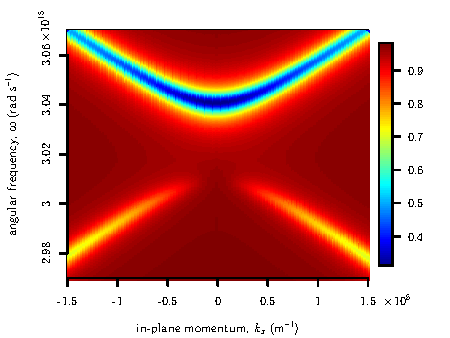
\includegraphics[]{figure-bandedgecoupling-band1}\label{fig:couplingbandedgesB}}
\subfigure[$\psi_2=-90^\circ$]{% Created by tikzDevice version 0.6.2-92-0ad2792 on 2013-01-22 18:38:21
% !TEX encoding = UTF-8 Unicode
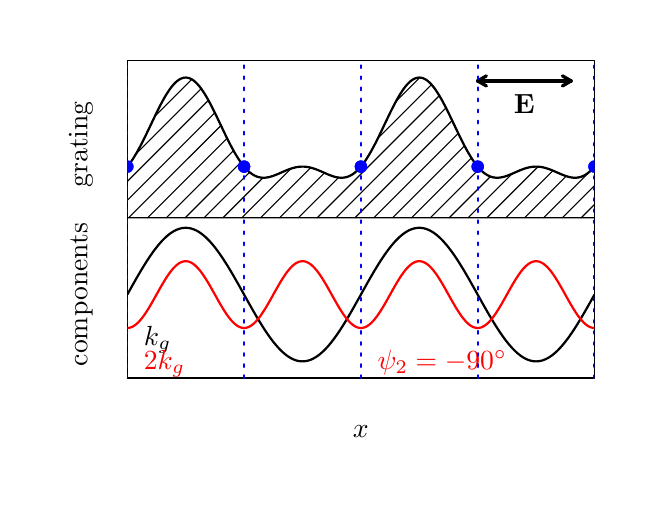
\begin{tikzpicture}[x=1pt,y=1pt]
\definecolor[named]{fillColor}{rgb}{1.00,1.00,1.00}
\path[use as bounding box,fill=fillColor,fill opacity=0.00] (0,0) rectangle (216.81,162.61);
\begin{scope}
\path[clip] ( 36.00, 36.00) rectangle (204.81,150.61);
\definecolor[named]{drawColor}{rgb}{0.00,0.00,0.00}

\path[draw=drawColor,line width= 0.8pt,line join=round,line cap=round] ( 36.00,112.40) --
	( 36.34,112.82) --
	( 36.68,113.26) --
	( 37.01,113.71) --
	( 37.35,114.19) --
	( 37.69,114.68) --
	( 38.03,115.19) --
	( 38.37,115.72) --
	( 38.71,116.27) --
	( 39.04,116.83) --
	( 39.38,117.41) --
	( 39.72,118.01) --
	( 40.06,118.62) --
	( 40.40,119.24) --
	( 40.74,119.88) --
	( 41.07,120.53) --
	( 41.41,121.19) --
	( 41.75,121.86) --
	( 42.09,122.53) --
	( 42.43,123.22) --
	( 42.77,123.92) --
	( 43.10,124.62) --
	( 43.44,125.32) --
	( 43.78,126.03) --
	( 44.12,126.74) --
	( 44.46,127.45) --
	( 44.80,128.17) --
	( 45.13,128.88) --
	( 45.47,129.59) --
	( 45.81,130.29) --
	( 46.15,131.00) --
	( 46.49,131.69) --
	( 46.83,132.38) --
	( 47.16,133.06) --
	( 47.50,133.73) --
	( 47.84,134.39) --
	( 48.18,135.04) --
	( 48.52,135.68) --
	( 48.86,136.30) --
	( 49.19,136.91) --
	( 49.53,137.50) --
	( 49.87,138.07) --
	( 50.21,138.63) --
	( 50.55,139.16) --
	( 50.89,139.68) --
	( 51.22,140.17) --
	( 51.56,140.64) --
	( 51.90,141.09) --
	( 52.24,141.52) --
	( 52.58,141.91) --
	( 52.91,142.29) --
	( 53.25,142.64) --
	( 53.59,142.96) --
	( 53.93,143.25) --
	( 54.27,143.51) --
	( 54.61,143.75) --
	( 54.94,143.96) --
	( 55.28,144.14) --
	( 55.62,144.28) --
	( 55.96,144.40) --
	( 56.30,144.49) --
	( 56.64,144.55) --
	( 56.97,144.57) --
	( 57.31,144.57) --
	( 57.65,144.54) --
	( 57.99,144.47) --
	( 58.33,144.38) --
	( 58.67,144.25) --
	( 59.00,144.09) --
	( 59.34,143.91) --
	( 59.68,143.69) --
	( 60.02,143.45) --
	( 60.36,143.18) --
	( 60.70,142.88) --
	( 61.03,142.55) --
	( 61.37,142.20) --
	( 61.71,141.82) --
	( 62.05,141.41) --
	( 62.39,140.98) --
	( 62.73,140.53) --
	( 63.06,140.05) --
	( 63.40,139.55) --
	( 63.74,139.03) --
	( 64.08,138.49) --
	( 64.42,137.93) --
	( 64.76,137.35) --
	( 65.09,136.76) --
	( 65.43,136.15) --
	( 65.77,135.52) --
	( 66.11,134.88) --
	( 66.45,134.23) --
	( 66.78,133.57) --
	( 67.12,132.89) --
	( 67.46,132.21) --
	( 67.80,131.52) --
	( 68.14,130.82) --
	( 68.48,130.12) --
	( 68.81,129.41) --
	( 69.15,128.70) --
	( 69.49,127.99) --
	( 69.83,127.27) --
	( 70.17,126.56) --
	( 70.51,125.85) --
	( 70.84,125.14) --
	( 71.18,124.44) --
	( 71.52,123.74) --
	( 71.86,123.05) --
	( 72.20,122.36) --
	( 72.54,121.69) --
	( 72.87,121.02) --
	( 73.21,120.36) --
	( 73.55,119.72) --
	( 73.89,119.08) --
	( 74.23,118.46) --
	( 74.57,117.86) --
	( 74.90,117.27) --
	( 75.24,116.69) --
	( 75.58,116.13) --
	( 75.92,115.59) --
	( 76.26,115.06) --
	( 76.60,114.55) --
	( 76.93,114.06) --
	( 77.27,113.60) --
	( 77.61,113.14) --
	( 77.95,112.71) --
	( 78.29,112.30) --
	( 78.63,111.91) --
	( 78.96,111.55) --
	( 79.30,111.20) --
	( 79.64,110.87) --
	( 79.98,110.56) --
	( 80.32,110.28) --
	( 80.66,110.01) --
	( 80.99,109.77) --
	( 81.33,109.55) --
	( 81.67,109.35) --
	( 82.01,109.17) --
	( 82.35,109.00) --
	( 82.68,108.86) --
	( 83.02,108.74) --
	( 83.36,108.64) --
	( 83.70,108.55) --
	( 84.04,108.48) --
	( 84.38,108.43) --
	( 84.71,108.40) --
	( 85.05,108.39) --
	( 85.39,108.39) --
	( 85.73,108.40) --
	( 86.07,108.43) --
	( 86.41,108.47) --
	( 86.74,108.53) --
	( 87.08,108.59) --
	( 87.42,108.67) --
	( 87.76,108.76) --
	( 88.10,108.86) --
	( 88.44,108.97) --
	( 88.77,109.08) --
	( 89.11,109.20) --
	( 89.45,109.33) --
	( 89.79,109.47) --
	( 90.13,109.61) --
	( 90.47,109.75) --
	( 90.80,109.89) --
	( 91.14,110.04) --
	( 91.48,110.19) --
	( 91.82,110.34) --
	( 92.16,110.49) --
	( 92.50,110.64) --
	( 92.83,110.78) --
	( 93.17,110.93) --
	( 93.51,111.07) --
	( 93.85,111.20) --
	( 94.19,111.33) --
	( 94.53,111.46) --
	( 94.86,111.58) --
	( 95.20,111.70) --
	( 95.54,111.80) --
	( 95.88,111.90) --
	( 96.22,111.99) --
	( 96.56,112.08) --
	( 96.89,112.15) --
	( 97.23,112.22) --
	( 97.57,112.27) --
	( 97.91,112.32) --
	( 98.25,112.36) --
	( 98.58,112.38) --
	( 98.92,112.40) --
	( 99.26,112.40) --
	( 99.60,112.40) --
	( 99.94,112.39) --
	(100.28,112.36) --
	(100.61,112.33) --
	(100.95,112.28) --
	(101.29,112.23) --
	(101.63,112.17) --
	(101.97,112.10) --
	(102.31,112.01) --
	(102.64,111.93) --
	(102.98,111.83) --
	(103.32,111.72) --
	(103.66,111.61) --
	(104.00,111.49) --
	(104.34,111.37) --
	(104.67,111.24) --
	(105.01,111.10) --
	(105.35,110.96) --
	(105.69,110.82) --
	(106.03,110.67) --
	(106.37,110.53) --
	(106.70,110.38) --
	(107.04,110.23) --
	(107.38,110.08) --
	(107.72,109.93) --
	(108.06,109.78) --
	(108.40,109.64) --
	(108.73,109.50) --
	(109.07,109.37) --
	(109.41,109.24) --
	(109.75,109.11) --
	(110.09,108.99) --
	(110.43,108.88) --
	(110.76,108.78) --
	(111.10,108.69) --
	(111.44,108.61) --
	(111.78,108.54) --
	(112.12,108.48) --
	(112.46,108.44) --
	(112.79,108.41) --
	(113.13,108.39) --
	(113.47,108.38) --
	(113.81,108.40) --
	(114.15,108.43) --
	(114.48,108.47) --
	(114.82,108.53) --
	(115.16,108.61) --
	(115.50,108.71) --
	(115.84,108.83) --
	(116.18,108.97) --
	(116.51,109.12) --
	(116.85,109.30) --
	(117.19,109.50) --
	(117.53,109.71) --
	(117.87,109.95) --
	(118.21,110.21) --
	(118.54,110.49) --
	(118.88,110.79) --
	(119.22,111.11) --
	(119.56,111.46) --
	(119.90,111.82) --
	(120.24,112.20) --
	(120.57,112.61) --
	(120.91,113.04) --
	(121.25,113.48) --
	(121.59,113.95) --
	(121.93,114.43) --
	(122.27,114.93) --
	(122.60,115.45) --
	(122.94,115.99) --
	(123.28,116.55) --
	(123.62,117.12) --
	(123.96,117.71) --
	(124.30,118.31) --
	(124.63,118.93) --
	(124.97,119.56) --
	(125.31,120.20) --
	(125.65,120.85) --
	(125.99,121.52) --
	(126.33,122.19) --
	(126.66,122.88) --
	(127.00,123.57) --
	(127.34,124.26) --
	(127.68,124.97) --
	(128.02,125.67) --
	(128.35,126.38) --
	(128.69,127.10) --
	(129.03,127.81) --
	(129.37,128.52) --
	(129.71,129.23) --
	(130.05,129.94) --
	(130.38,130.65) --
	(130.72,131.34) --
	(131.06,132.04) --
	(131.40,132.72) --
	(131.74,133.40) --
	(132.08,134.07) --
	(132.41,134.72) --
	(132.75,135.36) --
	(133.09,135.99) --
	(133.43,136.61) --
	(133.77,137.21) --
	(134.11,137.79) --
	(134.44,138.35) --
	(134.78,138.90) --
	(135.12,139.42) --
	(135.46,139.93) --
	(135.80,140.41) --
	(136.14,140.87) --
	(136.47,141.31) --
	(136.81,141.72) --
	(137.15,142.11) --
	(137.49,142.47) --
	(137.83,142.80) --
	(138.17,143.11) --
	(138.50,143.39) --
	(138.84,143.64) --
	(139.18,143.86) --
	(139.52,144.05) --
	(139.86,144.21) --
	(140.20,144.35) --
	(140.53,144.45) --
	(140.87,144.52) --
	(141.21,144.56) --
	(141.55,144.58) --
	(141.89,144.56) --
	(142.23,144.51) --
	(142.56,144.43) --
	(142.90,144.32) --
	(143.24,144.18) --
	(143.58,144.01) --
	(143.92,143.81) --
	(144.25,143.58) --
	(144.59,143.32) --
	(144.93,143.03) --
	(145.27,142.72) --
	(145.61,142.38) --
	(145.95,142.01) --
	(146.28,141.62) --
	(146.62,141.20) --
	(146.96,140.76) --
	(147.30,140.29) --
	(147.64,139.80) --
	(147.98,139.29) --
	(148.31,138.76) --
	(148.65,138.21) --
	(148.99,137.65) --
	(149.33,137.06) --
	(149.67,136.46) --
	(150.01,135.84) --
	(150.34,135.20) --
	(150.68,134.56) --
	(151.02,133.90) --
	(151.36,133.23) --
	(151.70,132.55) --
	(152.04,131.86) --
	(152.37,131.17) --
	(152.71,130.47) --
	(153.05,129.76) --
	(153.39,129.06) --
	(153.73,128.34) --
	(154.07,127.63) --
	(154.40,126.92) --
	(154.74,126.21) --
	(155.08,125.50) --
	(155.42,124.79) --
	(155.76,124.09) --
	(156.10,123.39) --
	(156.43,122.71) --
	(156.77,122.02) --
	(157.11,121.35) --
	(157.45,120.69) --
	(157.79,120.04) --
	(158.13,119.40) --
	(158.46,118.77) --
	(158.80,118.16) --
	(159.14,117.56) --
	(159.48,116.98) --
	(159.82,116.41) --
	(160.15,115.86) --
	(160.49,115.32) --
	(160.83,114.80) --
	(161.17,114.31) --
	(161.51,113.83) --
	(161.85,113.37) --
	(162.18,112.93) --
	(162.52,112.51) --
	(162.86,112.11) --
	(163.20,111.73) --
	(163.54,111.37) --
	(163.88,111.03) --
	(164.21,110.71) --
	(164.55,110.42) --
	(164.89,110.14) --
	(165.23,109.89) --
	(165.57,109.66) --
	(165.91,109.45) --
	(166.24,109.25) --
	(166.58,109.08) --
	(166.92,108.93) --
	(167.26,108.80) --
	(167.60,108.69) --
	(167.94,108.59) --
	(168.27,108.52) --
	(168.61,108.46) --
	(168.95,108.42) --
	(169.29,108.39) --
	(169.63,108.38) --
	(169.97,108.39) --
	(170.30,108.41) --
	(170.64,108.45) --
	(170.98,108.50) --
	(171.32,108.56) --
	(171.66,108.63) --
	(172.00,108.71) --
	(172.33,108.81) --
	(172.67,108.91) --
	(173.01,109.02) --
	(173.35,109.14) --
	(173.69,109.27) --
	(174.03,109.40) --
	(174.36,109.54) --
	(174.70,109.68) --
	(175.04,109.82) --
	(175.38,109.97) --
	(175.72,110.12) --
	(176.05,110.27) --
	(176.39,110.41) --
	(176.73,110.56) --
	(177.07,110.71) --
	(177.41,110.86) --
	(177.75,111.00) --
	(178.08,111.14) --
	(178.42,111.27) --
	(178.76,111.40) --
	(179.10,111.52) --
	(179.44,111.64) --
	(179.78,111.75) --
	(180.11,111.85) --
	(180.45,111.95) --
	(180.79,112.04) --
	(181.13,112.11) --
	(181.47,112.18) --
	(181.81,112.25) --
	(182.14,112.30) --
	(182.48,112.34) --
	(182.82,112.37) --
	(183.16,112.39) --
	(183.50,112.40) --
	(183.84,112.40) --
	(184.17,112.40) --
	(184.51,112.38) --
	(184.85,112.35) --
	(185.19,112.31) --
	(185.53,112.26) --
	(185.87,112.20) --
	(186.20,112.13) --
	(186.54,112.06) --
	(186.88,111.97) --
	(187.22,111.88) --
	(187.56,111.78) --
	(187.90,111.67) --
	(188.23,111.55) --
	(188.57,111.43) --
	(188.91,111.30) --
	(189.25,111.17) --
	(189.59,111.03) --
	(189.92,110.89) --
	(190.26,110.75) --
	(190.60,110.60) --
	(190.94,110.45) --
	(191.28,110.30) --
	(191.62,110.15) --
	(191.95,110.00) --
	(192.29,109.86) --
	(192.63,109.71) --
	(192.97,109.57) --
	(193.31,109.43) --
	(193.65,109.30) --
	(193.98,109.17) --
	(194.32,109.05) --
	(194.66,108.94) --
	(195.00,108.83) --
	(195.34,108.74) --
	(195.68,108.65) --
	(196.01,108.57) --
	(196.35,108.51) --
	(196.69,108.46) --
	(197.03,108.42) --
	(197.37,108.39) --
	(197.71,108.38) --
	(198.04,108.39) --
	(198.38,108.41) --
	(198.72,108.45) --
	(199.06,108.50) --
	(199.40,108.57) --
	(199.74,108.66) --
	(200.07,108.77) --
	(200.41,108.90) --
	(200.75,109.04) --
	(201.09,109.21) --
	(201.43,109.40) --
	(201.77,109.60) --
	(202.10,109.83) --
	(202.44,110.08) --
	(202.78,110.35) --
	(203.12,110.64) --
	(203.46,110.95) --
	(203.80,111.28) --
	(204.13,111.64) --
	(204.47,112.01) --
	(204.81,112.40);
\end{scope}
\begin{scope}
\path[clip] (  0.00,  0.00) rectangle (216.81,162.61);
\definecolor[named]{drawColor}{rgb}{0.00,0.00,0.00}

\path[draw=drawColor,line width= 0.4pt,line join=round,line cap=round] ( 36.00, 36.00) --
	(204.81, 36.00) --
	(204.81,150.61) --
	( 36.00,150.61) --
	( 36.00, 36.00);
\end{scope}
\begin{scope}
\path[clip] (  0.00,  0.00) rectangle (216.81,162.61);
\definecolor[named]{drawColor}{rgb}{0.00,0.00,0.00}

\node[text=drawColor,rotate= 90.00,anchor=base,inner sep=0pt, outer sep=0pt, scale=  1.00] at ( 21.60,120.45) {grating};

\node[text=drawColor,rotate= 90.00,anchor=base,inner sep=0pt, outer sep=0pt, scale=  1.00] at ( 21.60, 66.16) {components};

\node[text=drawColor,anchor=base,inner sep=0pt, outer sep=0pt, scale=  1.00] at (120.41, 14.40) {$x$};
\end{scope}
\begin{scope}
\path[clip] ( 36.00, 36.00) rectangle (204.81,150.61);
\definecolor[named]{drawColor}{rgb}{0.00,0.00,0.00}

\node[text=drawColor,anchor=base west,inner sep=0pt, outer sep=0pt, scale=  1.00] at ( 42.00, 47.94) {$k_g$};
\definecolor[named]{drawColor}{rgb}{1.00,0.00,0.00}

\node[text=drawColor,anchor=base west,inner sep=0pt, outer sep=0pt, scale=  1.00] at ( 42.00, 39.25) {2$k_g$};

\node[text=drawColor,anchor=base west,inner sep=0pt, outer sep=0pt, scale=  1.00] at (126.41, 39.25) {$\psi_2=-90^\circ$};
\definecolor[named]{drawColor}{rgb}{0.00,0.00,0.00}

\path[draw=drawColor,line width= 1.2pt,line join=round,line cap=round] (162.61,143.37) -- (196.37,143.37);

\path[draw=drawColor,line width= 1.2pt,line join=round,line cap=round] (165.74,145.18) --
	(162.61,143.37) --
	(165.74,141.56);

\path[draw=drawColor,line width= 1.2pt,line join=round,line cap=round] (193.24,141.56) --
	(196.37,143.37) --
	(193.24,145.18);

\node[text=drawColor,anchor=base,inner sep=0pt, outer sep=0pt, scale=  1.00] at (179.49,131.63) {$\mathbf{E}$};

\path[draw=drawColor,line width= 0.4pt,line join=round,line cap=round] ( 45.98,130.65) -- ( 59.28,143.95);

\path[draw=drawColor,line width= 0.4pt,line join=round,line cap=round] ( 39.14,117.00) -- ( 62.70,140.56);

\path[draw=drawColor,line width= 0.4pt,line join=round,line cap=round] ( 36.00,107.04) -- ( 65.32,136.36);

\path[draw=drawColor,line width= 0.4pt,line join=round,line cap=round] ( 36.00,100.23) -- ( 67.63,131.86);

\path[draw=drawColor,line width= 0.4pt,line join=round,line cap=round] ( 36.49, 93.91) -- ( 69.84,127.25);

\path[draw=drawColor,line width= 0.4pt,line join=round,line cap=round] ( 43.31, 93.91) -- ( 72.05,122.65);

\path[draw=drawColor,line width= 0.4pt,line join=round,line cap=round] ( 50.12, 93.91) -- ( 74.39,118.18);

\path[draw=drawColor,line width= 0.4pt,line join=round,line cap=round] ( 56.93, 93.91) -- ( 77.00,113.97);

\path[draw=drawColor,line width= 0.4pt,line join=round,line cap=round] ( 63.75, 93.91) -- ( 80.21,110.37);

\path[draw=drawColor,line width= 0.4pt,line join=round,line cap=round] ( 70.56, 93.91) -- ( 85.04,108.39);

\path[draw=drawColor,line width= 0.4pt,line join=round,line cap=round] ( 77.37, 93.91) -- ( 95.14,111.68);

\path[draw=drawColor,line width= 0.4pt,line join=round,line cap=round] ( 84.19, 93.91) -- (102.30,112.02);

\path[draw=drawColor,line width= 0.4pt,line join=round,line cap=round] ( 91.00, 93.91) -- (107.24,110.14);

\path[draw=drawColor,line width= 0.4pt,line join=round,line cap=round] (133.10,136.00) -- (141.66,144.57);

\path[draw=drawColor,line width= 0.4pt,line join=round,line cap=round] ( 97.82, 93.91) -- (112.36,108.45);

\path[draw=drawColor,line width= 0.4pt,line join=round,line cap=round] (126.54,122.64) -- (145.93,142.02);

\path[draw=drawColor,line width= 0.4pt,line join=round,line cap=round] (104.63, 93.91) -- (148.76,138.04);

\path[draw=drawColor,line width= 0.4pt,line join=round,line cap=round] (111.44, 93.91) -- (151.16,133.62);

\path[draw=drawColor,line width= 0.4pt,line join=round,line cap=round] (118.26, 93.91) -- (153.39,129.04);

\path[draw=drawColor,line width= 0.4pt,line join=round,line cap=round] (125.07, 93.91) -- (155.59,124.43);

\path[draw=drawColor,line width= 0.4pt,line join=round,line cap=round] (131.88, 93.91) -- (157.87,119.89);

\path[draw=drawColor,line width= 0.4pt,line join=round,line cap=round] (138.70, 93.91) -- (160.35,115.55);

\path[draw=drawColor,line width= 0.4pt,line join=round,line cap=round] (145.51, 93.91) -- (163.26,111.66);

\path[draw=drawColor,line width= 0.4pt,line join=round,line cap=round] (152.32, 93.91) -- (167.23,108.81);

\path[draw=drawColor,line width= 0.4pt,line join=round,line cap=round] (159.14, 93.91) -- (175.06,109.83);

\path[draw=drawColor,line width= 0.4pt,line join=round,line cap=round] (165.95, 93.91) -- (184.43,112.38);

\path[draw=drawColor,line width= 0.4pt,line join=round,line cap=round] (172.77, 93.91) -- (189.80,110.94);

\path[draw=drawColor,line width= 0.4pt,line join=round,line cap=round] (179.58, 93.91) -- (194.62,108.95);

\path[draw=drawColor,line width= 0.4pt,line join=round,line cap=round] (186.39, 93.91) -- (203.20,110.71);

\path[draw=drawColor,line width= 0.4pt,line join=round,line cap=round] (204.24,111.75) -- (204.83,112.34);

\path[draw=drawColor,line width= 0.4pt,line join=round,line cap=round] (193.21, 93.91) -- (206.46,107.16);

\path[draw=drawColor,line width= 0.4pt,line join=round,line cap=round] (200.02, 93.91) -- (208.09,101.98);

\path[draw=drawColor,line width= 0.4pt,line join=round,line cap=round] (206.83, 93.91) -- (209.72, 96.80);

\path[draw=drawColor,line width= 0.4pt,line join=round,line cap=round] ( 36.00,112.40) --
	( 36.34,112.82) --
	( 36.68,113.26) --
	( 37.01,113.71) --
	( 37.35,114.19) --
	( 37.69,114.68) --
	( 38.03,115.19) --
	( 38.37,115.72) --
	( 38.71,116.27) --
	( 39.04,116.83) --
	( 39.38,117.41) --
	( 39.72,118.01) --
	( 40.06,118.62) --
	( 40.40,119.24) --
	( 40.74,119.88) --
	( 41.07,120.53) --
	( 41.41,121.19) --
	( 41.75,121.86) --
	( 42.09,122.53) --
	( 42.43,123.22) --
	( 42.77,123.92) --
	( 43.10,124.62) --
	( 43.44,125.32) --
	( 43.78,126.03) --
	( 44.12,126.74) --
	( 44.46,127.45) --
	( 44.80,128.17) --
	( 45.13,128.88) --
	( 45.47,129.59) --
	( 45.81,130.29) --
	( 46.15,131.00) --
	( 46.49,131.69) --
	( 46.83,132.38) --
	( 47.16,133.06) --
	( 47.50,133.73) --
	( 47.84,134.39) --
	( 48.18,135.04) --
	( 48.52,135.68) --
	( 48.86,136.30) --
	( 49.19,136.91) --
	( 49.53,137.50) --
	( 49.87,138.07) --
	( 50.21,138.63) --
	( 50.55,139.16) --
	( 50.89,139.68) --
	( 51.22,140.17) --
	( 51.56,140.64) --
	( 51.90,141.09) --
	( 52.24,141.52) --
	( 52.58,141.91) --
	( 52.91,142.29) --
	( 53.25,142.64) --
	( 53.59,142.96) --
	( 53.93,143.25) --
	( 54.27,143.51) --
	( 54.61,143.75) --
	( 54.94,143.96) --
	( 55.28,144.14) --
	( 55.62,144.28) --
	( 55.96,144.40) --
	( 56.30,144.49) --
	( 56.64,144.55) --
	( 56.97,144.57) --
	( 57.31,144.57) --
	( 57.65,144.54) --
	( 57.99,144.47) --
	( 58.33,144.38) --
	( 58.67,144.25) --
	( 59.00,144.09) --
	( 59.34,143.91) --
	( 59.68,143.69) --
	( 60.02,143.45) --
	( 60.36,143.18) --
	( 60.70,142.88) --
	( 61.03,142.55) --
	( 61.37,142.20) --
	( 61.71,141.82) --
	( 62.05,141.41) --
	( 62.39,140.98) --
	( 62.73,140.53) --
	( 63.06,140.05) --
	( 63.40,139.55) --
	( 63.74,139.03) --
	( 64.08,138.49) --
	( 64.42,137.93) --
	( 64.76,137.35) --
	( 65.09,136.76) --
	( 65.43,136.15) --
	( 65.77,135.52) --
	( 66.11,134.88) --
	( 66.45,134.23) --
	( 66.78,133.57) --
	( 67.12,132.89) --
	( 67.46,132.21) --
	( 67.80,131.52) --
	( 68.14,130.82) --
	( 68.48,130.12) --
	( 68.81,129.41) --
	( 69.15,128.70) --
	( 69.49,127.99) --
	( 69.83,127.27) --
	( 70.17,126.56) --
	( 70.51,125.85) --
	( 70.84,125.14) --
	( 71.18,124.44) --
	( 71.52,123.74) --
	( 71.86,123.05) --
	( 72.20,122.36) --
	( 72.54,121.69) --
	( 72.87,121.02) --
	( 73.21,120.36) --
	( 73.55,119.72) --
	( 73.89,119.08) --
	( 74.23,118.46) --
	( 74.57,117.86) --
	( 74.90,117.27) --
	( 75.24,116.69) --
	( 75.58,116.13) --
	( 75.92,115.59) --
	( 76.26,115.06) --
	( 76.60,114.55) --
	( 76.93,114.06) --
	( 77.27,113.60) --
	( 77.61,113.14) --
	( 77.95,112.71) --
	( 78.29,112.30) --
	( 78.63,111.91) --
	( 78.96,111.55) --
	( 79.30,111.20) --
	( 79.64,110.87) --
	( 79.98,110.56) --
	( 80.32,110.28) --
	( 80.66,110.01) --
	( 80.99,109.77) --
	( 81.33,109.55) --
	( 81.67,109.35) --
	( 82.01,109.17) --
	( 82.35,109.00) --
	( 82.68,108.86) --
	( 83.02,108.74) --
	( 83.36,108.64) --
	( 83.70,108.55) --
	( 84.04,108.48) --
	( 84.38,108.43) --
	( 84.71,108.40) --
	( 85.05,108.39) --
	( 85.39,108.39) --
	( 85.73,108.40) --
	( 86.07,108.43) --
	( 86.41,108.47) --
	( 86.74,108.53) --
	( 87.08,108.59) --
	( 87.42,108.67) --
	( 87.76,108.76) --
	( 88.10,108.86) --
	( 88.44,108.97) --
	( 88.77,109.08) --
	( 89.11,109.20) --
	( 89.45,109.33) --
	( 89.79,109.47) --
	( 90.13,109.61) --
	( 90.47,109.75) --
	( 90.80,109.89) --
	( 91.14,110.04) --
	( 91.48,110.19) --
	( 91.82,110.34) --
	( 92.16,110.49) --
	( 92.50,110.64) --
	( 92.83,110.78) --
	( 93.17,110.93) --
	( 93.51,111.07) --
	( 93.85,111.20) --
	( 94.19,111.33) --
	( 94.53,111.46) --
	( 94.86,111.58) --
	( 95.20,111.70) --
	( 95.54,111.80) --
	( 95.88,111.90) --
	( 96.22,111.99) --
	( 96.56,112.08) --
	( 96.89,112.15) --
	( 97.23,112.22) --
	( 97.57,112.27) --
	( 97.91,112.32) --
	( 98.25,112.36) --
	( 98.58,112.38) --
	( 98.92,112.40) --
	( 99.26,112.40) --
	( 99.60,112.40) --
	( 99.94,112.39) --
	(100.28,112.36) --
	(100.61,112.33) --
	(100.95,112.28) --
	(101.29,112.23) --
	(101.63,112.17) --
	(101.97,112.10) --
	(102.31,112.01) --
	(102.64,111.93) --
	(102.98,111.83) --
	(103.32,111.72) --
	(103.66,111.61) --
	(104.00,111.49) --
	(104.34,111.37) --
	(104.67,111.24) --
	(105.01,111.10) --
	(105.35,110.96) --
	(105.69,110.82) --
	(106.03,110.67) --
	(106.37,110.53) --
	(106.70,110.38) --
	(107.04,110.23) --
	(107.38,110.08) --
	(107.72,109.93) --
	(108.06,109.78) --
	(108.40,109.64) --
	(108.73,109.50) --
	(109.07,109.37) --
	(109.41,109.24) --
	(109.75,109.11) --
	(110.09,108.99) --
	(110.43,108.88) --
	(110.76,108.78) --
	(111.10,108.69) --
	(111.44,108.61) --
	(111.78,108.54) --
	(112.12,108.48) --
	(112.46,108.44) --
	(112.79,108.41) --
	(113.13,108.39) --
	(113.47,108.38) --
	(113.81,108.40) --
	(114.15,108.43) --
	(114.48,108.47) --
	(114.82,108.53) --
	(115.16,108.61) --
	(115.50,108.71) --
	(115.84,108.83) --
	(116.18,108.97) --
	(116.51,109.12) --
	(116.85,109.30) --
	(117.19,109.50) --
	(117.53,109.71) --
	(117.87,109.95) --
	(118.21,110.21) --
	(118.54,110.49) --
	(118.88,110.79) --
	(119.22,111.11) --
	(119.56,111.46) --
	(119.90,111.82) --
	(120.24,112.20) --
	(120.57,112.61) --
	(120.91,113.04) --
	(121.25,113.48) --
	(121.59,113.95) --
	(121.93,114.43) --
	(122.27,114.93) --
	(122.60,115.45) --
	(122.94,115.99) --
	(123.28,116.55) --
	(123.62,117.12) --
	(123.96,117.71) --
	(124.30,118.31) --
	(124.63,118.93) --
	(124.97,119.56) --
	(125.31,120.20) --
	(125.65,120.85) --
	(125.99,121.52) --
	(126.33,122.19) --
	(126.66,122.88) --
	(127.00,123.57) --
	(127.34,124.26) --
	(127.68,124.97) --
	(128.02,125.67) --
	(128.35,126.38) --
	(128.69,127.10) --
	(129.03,127.81) --
	(129.37,128.52) --
	(129.71,129.23) --
	(130.05,129.94) --
	(130.38,130.65) --
	(130.72,131.34) --
	(131.06,132.04) --
	(131.40,132.72) --
	(131.74,133.40) --
	(132.08,134.07) --
	(132.41,134.72) --
	(132.75,135.36) --
	(133.09,135.99) --
	(133.43,136.61) --
	(133.77,137.21) --
	(134.11,137.79) --
	(134.44,138.35) --
	(134.78,138.90) --
	(135.12,139.42) --
	(135.46,139.93) --
	(135.80,140.41) --
	(136.14,140.87) --
	(136.47,141.31) --
	(136.81,141.72) --
	(137.15,142.11) --
	(137.49,142.47) --
	(137.83,142.80) --
	(138.17,143.11) --
	(138.50,143.39) --
	(138.84,143.64) --
	(139.18,143.86) --
	(139.52,144.05) --
	(139.86,144.21) --
	(140.20,144.35) --
	(140.53,144.45) --
	(140.87,144.52) --
	(141.21,144.56) --
	(141.55,144.58) --
	(141.89,144.56) --
	(142.23,144.51) --
	(142.56,144.43) --
	(142.90,144.32) --
	(143.24,144.18) --
	(143.58,144.01) --
	(143.92,143.81) --
	(144.25,143.58) --
	(144.59,143.32) --
	(144.93,143.03) --
	(145.27,142.72) --
	(145.61,142.38) --
	(145.95,142.01) --
	(146.28,141.62) --
	(146.62,141.20) --
	(146.96,140.76) --
	(147.30,140.29) --
	(147.64,139.80) --
	(147.98,139.29) --
	(148.31,138.76) --
	(148.65,138.21) --
	(148.99,137.65) --
	(149.33,137.06) --
	(149.67,136.46) --
	(150.01,135.84) --
	(150.34,135.20) --
	(150.68,134.56) --
	(151.02,133.90) --
	(151.36,133.23) --
	(151.70,132.55) --
	(152.04,131.86) --
	(152.37,131.17) --
	(152.71,130.47) --
	(153.05,129.76) --
	(153.39,129.06) --
	(153.73,128.34) --
	(154.07,127.63) --
	(154.40,126.92) --
	(154.74,126.21) --
	(155.08,125.50) --
	(155.42,124.79) --
	(155.76,124.09) --
	(156.10,123.39) --
	(156.43,122.71) --
	(156.77,122.02) --
	(157.11,121.35) --
	(157.45,120.69) --
	(157.79,120.04) --
	(158.13,119.40) --
	(158.46,118.77) --
	(158.80,118.16) --
	(159.14,117.56) --
	(159.48,116.98) --
	(159.82,116.41) --
	(160.15,115.86) --
	(160.49,115.32) --
	(160.83,114.80) --
	(161.17,114.31) --
	(161.51,113.83) --
	(161.85,113.37) --
	(162.18,112.93) --
	(162.52,112.51) --
	(162.86,112.11) --
	(163.20,111.73) --
	(163.54,111.37) --
	(163.88,111.03) --
	(164.21,110.71) --
	(164.55,110.42) --
	(164.89,110.14) --
	(165.23,109.89) --
	(165.57,109.66) --
	(165.91,109.45) --
	(166.24,109.25) --
	(166.58,109.08) --
	(166.92,108.93) --
	(167.26,108.80) --
	(167.60,108.69) --
	(167.94,108.59) --
	(168.27,108.52) --
	(168.61,108.46) --
	(168.95,108.42) --
	(169.29,108.39) --
	(169.63,108.38) --
	(169.97,108.39) --
	(170.30,108.41) --
	(170.64,108.45) --
	(170.98,108.50) --
	(171.32,108.56) --
	(171.66,108.63) --
	(172.00,108.71) --
	(172.33,108.81) --
	(172.67,108.91) --
	(173.01,109.02) --
	(173.35,109.14) --
	(173.69,109.27) --
	(174.03,109.40) --
	(174.36,109.54) --
	(174.70,109.68) --
	(175.04,109.82) --
	(175.38,109.97) --
	(175.72,110.12) --
	(176.05,110.27) --
	(176.39,110.41) --
	(176.73,110.56) --
	(177.07,110.71) --
	(177.41,110.86) --
	(177.75,111.00) --
	(178.08,111.14) --
	(178.42,111.27) --
	(178.76,111.40) --
	(179.10,111.52) --
	(179.44,111.64) --
	(179.78,111.75) --
	(180.11,111.85) --
	(180.45,111.95) --
	(180.79,112.04) --
	(181.13,112.11) --
	(181.47,112.18) --
	(181.81,112.25) --
	(182.14,112.30) --
	(182.48,112.34) --
	(182.82,112.37) --
	(183.16,112.39) --
	(183.50,112.40) --
	(183.84,112.40) --
	(184.17,112.40) --
	(184.51,112.38) --
	(184.85,112.35) --
	(185.19,112.31) --
	(185.53,112.26) --
	(185.87,112.20) --
	(186.20,112.13) --
	(186.54,112.06) --
	(186.88,111.97) --
	(187.22,111.88) --
	(187.56,111.78) --
	(187.90,111.67) --
	(188.23,111.55) --
	(188.57,111.43) --
	(188.91,111.30) --
	(189.25,111.17) --
	(189.59,111.03) --
	(189.92,110.89) --
	(190.26,110.75) --
	(190.60,110.60) --
	(190.94,110.45) --
	(191.28,110.30) --
	(191.62,110.15) --
	(191.95,110.00) --
	(192.29,109.86) --
	(192.63,109.71) --
	(192.97,109.57) --
	(193.31,109.43) --
	(193.65,109.30) --
	(193.98,109.17) --
	(194.32,109.05) --
	(194.66,108.94) --
	(195.00,108.83) --
	(195.34,108.74) --
	(195.68,108.65) --
	(196.01,108.57) --
	(196.35,108.51) --
	(196.69,108.46) --
	(197.03,108.42) --
	(197.37,108.39) --
	(197.71,108.38) --
	(198.04,108.39) --
	(198.38,108.41) --
	(198.72,108.45) --
	(199.06,108.50) --
	(199.40,108.57) --
	(199.74,108.66) --
	(200.07,108.77) --
	(200.41,108.90) --
	(200.75,109.04) --
	(201.09,109.21) --
	(201.43,109.40) --
	(201.77,109.60) --
	(202.10,109.83) --
	(202.44,110.08) --
	(202.78,110.35) --
	(203.12,110.64) --
	(203.46,110.95) --
	(203.80,111.28) --
	(204.13,111.64) --
	(204.47,112.01) --
	(204.81,112.40) --
	(210.64, 93.91) --
	( 36.00, 93.91) --
	( 36.00,112.40);

\path[draw=drawColor,line width= 0.8pt,line join=round,line cap=round] ( 36.00, 66.16) --
	( 36.34, 66.77) --
	( 36.68, 67.37) --
	( 37.01, 67.98) --
	( 37.35, 68.59) --
	( 37.69, 69.19) --
	( 38.03, 69.79) --
	( 38.37, 70.39) --
	( 38.71, 70.99) --
	( 39.04, 71.58) --
	( 39.38, 72.17) --
	( 39.72, 72.76) --
	( 40.06, 73.34) --
	( 40.40, 73.92) --
	( 40.74, 74.49) --
	( 41.07, 75.06) --
	( 41.41, 75.62) --
	( 41.75, 76.18) --
	( 42.09, 76.73) --
	( 42.43, 77.27) --
	( 42.77, 77.80) --
	( 43.10, 78.33) --
	( 43.44, 78.85) --
	( 43.78, 79.37) --
	( 44.12, 79.87) --
	( 44.46, 80.37) --
	( 44.80, 80.85) --
	( 45.13, 81.33) --
	( 45.47, 81.80) --
	( 45.81, 82.26) --
	( 46.15, 82.70) --
	( 46.49, 83.14) --
	( 46.83, 83.57) --
	( 47.16, 83.98) --
	( 47.50, 84.39) --
	( 47.84, 84.78) --
	( 48.18, 85.16) --
	( 48.52, 85.53) --
	( 48.86, 85.88) --
	( 49.19, 86.23) --
	( 49.53, 86.56) --
	( 49.87, 86.88) --
	( 50.21, 87.18) --
	( 50.55, 87.47) --
	( 50.89, 87.75) --
	( 51.22, 88.01) --
	( 51.56, 88.27) --
	( 51.90, 88.50) --
	( 52.24, 88.72) --
	( 52.58, 88.93) --
	( 52.91, 89.13) --
	( 53.25, 89.30) --
	( 53.59, 89.47) --
	( 53.93, 89.62) --
	( 54.27, 89.75) --
	( 54.61, 89.87) --
	( 54.94, 89.98) --
	( 55.28, 90.07) --
	( 55.62, 90.14) --
	( 55.96, 90.20) --
	( 56.30, 90.24) --
	( 56.64, 90.27) --
	( 56.97, 90.29) --
	( 57.31, 90.28) --
	( 57.65, 90.27) --
	( 57.99, 90.24) --
	( 58.33, 90.19) --
	( 58.67, 90.12) --
	( 59.00, 90.05) --
	( 59.34, 89.95) --
	( 59.68, 89.84) --
	( 60.02, 89.72) --
	( 60.36, 89.58) --
	( 60.70, 89.43) --
	( 61.03, 89.26) --
	( 61.37, 89.08) --
	( 61.71, 88.88) --
	( 62.05, 88.67) --
	( 62.39, 88.44) --
	( 62.73, 88.20) --
	( 63.06, 87.95) --
	( 63.40, 87.68) --
	( 63.74, 87.40) --
	( 64.08, 87.11) --
	( 64.42, 86.80) --
	( 64.76, 86.48) --
	( 65.09, 86.14) --
	( 65.43, 85.80) --
	( 65.77, 85.44) --
	( 66.11, 85.06) --
	( 66.45, 84.68) --
	( 66.78, 84.29) --
	( 67.12, 83.88) --
	( 67.46, 83.46) --
	( 67.80, 83.03) --
	( 68.14, 82.59) --
	( 68.48, 82.14) --
	( 68.81, 81.68) --
	( 69.15, 81.21) --
	( 69.49, 80.73) --
	( 69.83, 80.24) --
	( 70.17, 79.75) --
	( 70.51, 79.24) --
	( 70.84, 78.72) --
	( 71.18, 78.20) --
	( 71.52, 77.67) --
	( 71.86, 77.13) --
	( 72.20, 76.59) --
	( 72.54, 76.04) --
	( 72.87, 75.48) --
	( 73.21, 74.92) --
	( 73.55, 74.35) --
	( 73.89, 73.77) --
	( 74.23, 73.20) --
	( 74.57, 72.61) --
	( 74.90, 72.02) --
	( 75.24, 71.43) --
	( 75.58, 70.84) --
	( 75.92, 70.24) --
	( 76.26, 69.64) --
	( 76.60, 69.04) --
	( 76.93, 68.44) --
	( 77.27, 67.83) --
	( 77.61, 67.22) --
	( 77.95, 66.62) --
	( 78.29, 66.01) --
	( 78.63, 65.40) --
	( 78.96, 64.79) --
	( 79.30, 64.19) --
	( 79.64, 63.58) --
	( 79.98, 62.98) --
	( 80.32, 62.38) --
	( 80.66, 61.78) --
	( 80.99, 61.18) --
	( 81.33, 60.59) --
	( 81.67, 60.00) --
	( 82.01, 59.42) --
	( 82.35, 58.83) --
	( 82.68, 58.26) --
	( 83.02, 57.69) --
	( 83.36, 57.12) --
	( 83.70, 56.56) --
	( 84.04, 56.01) --
	( 84.38, 55.46) --
	( 84.71, 54.92) --
	( 85.05, 54.38) --
	( 85.39, 53.86) --
	( 85.73, 53.34) --
	( 86.07, 52.83) --
	( 86.41, 52.32) --
	( 86.74, 51.83) --
	( 87.08, 51.35) --
	( 87.42, 50.87) --
	( 87.76, 50.41) --
	( 88.10, 49.95) --
	( 88.44, 49.51) --
	( 88.77, 49.07) --
	( 89.11, 48.65) --
	( 89.45, 48.24) --
	( 89.79, 47.84) --
	( 90.13, 47.45) --
	( 90.47, 47.07) --
	( 90.80, 46.70) --
	( 91.14, 46.35) --
	( 91.48, 46.01) --
	( 91.82, 45.68) --
	( 92.16, 45.37) --
	( 92.50, 45.06) --
	( 92.83, 44.78) --
	( 93.17, 44.50) --
	( 93.51, 44.24) --
	( 93.85, 43.99) --
	( 94.19, 43.76) --
	( 94.53, 43.54) --
	( 94.86, 43.34) --
	( 95.20, 43.15) --
	( 95.54, 42.97) --
	( 95.88, 42.81) --
	( 96.22, 42.67) --
	( 96.56, 42.54) --
	( 96.89, 42.42) --
	( 97.23, 42.32) --
	( 97.57, 42.23) --
	( 97.91, 42.16) --
	( 98.25, 42.11) --
	( 98.58, 42.07) --
	( 98.92, 42.04) --
	( 99.26, 42.03) --
	( 99.60, 42.04) --
	( 99.94, 42.06) --
	(100.28, 42.10) --
	(100.61, 42.15) --
	(100.95, 42.21) --
	(101.29, 42.30) --
	(101.63, 42.39) --
	(101.97, 42.50) --
	(102.31, 42.63) --
	(102.64, 42.77) --
	(102.98, 42.93) --
	(103.32, 43.10) --
	(103.66, 43.29) --
	(104.00, 43.49) --
	(104.34, 43.71) --
	(104.67, 43.93) --
	(105.01, 44.18) --
	(105.35, 44.44) --
	(105.69, 44.71) --
	(106.03, 44.99) --
	(106.37, 45.29) --
	(106.70, 45.60) --
	(107.04, 45.93) --
	(107.38, 46.26) --
	(107.72, 46.61) --
	(108.06, 46.98) --
	(108.40, 47.35) --
	(108.73, 47.74) --
	(109.07, 48.13) --
	(109.41, 48.54) --
	(109.75, 48.97) --
	(110.09, 49.40) --
	(110.43, 49.84) --
	(110.76, 50.29) --
	(111.10, 50.75) --
	(111.44, 51.23) --
	(111.78, 51.71) --
	(112.12, 52.20) --
	(112.46, 52.70) --
	(112.79, 53.21) --
	(113.13, 53.73) --
	(113.47, 54.25) --
	(113.81, 54.78) --
	(114.15, 55.32) --
	(114.48, 55.87) --
	(114.82, 56.42) --
	(115.16, 56.98) --
	(115.50, 57.54) --
	(115.84, 58.11) --
	(116.18, 58.69) --
	(116.51, 59.27) --
	(116.85, 59.85) --
	(117.19, 60.44) --
	(117.53, 61.03) --
	(117.87, 61.63) --
	(118.21, 62.23) --
	(118.54, 62.83) --
	(118.88, 63.43) --
	(119.22, 64.04) --
	(119.56, 64.64) --
	(119.90, 65.25) --
	(120.24, 65.86) --
	(120.57, 66.46) --
	(120.91, 67.07) --
	(121.25, 67.68) --
	(121.59, 68.28) --
	(121.93, 68.89) --
	(122.27, 69.49) --
	(122.60, 70.09) --
	(122.94, 70.69) --
	(123.28, 71.29) --
	(123.62, 71.88) --
	(123.96, 72.47) --
	(124.30, 73.05) --
	(124.63, 73.63) --
	(124.97, 74.21) --
	(125.31, 74.78) --
	(125.65, 75.34) --
	(125.99, 75.90) --
	(126.33, 76.45) --
	(126.66, 77.00) --
	(127.00, 77.54) --
	(127.34, 78.07) --
	(127.68, 78.59) --
	(128.02, 79.11) --
	(128.35, 79.62) --
	(128.69, 80.12) --
	(129.03, 80.61) --
	(129.37, 81.09) --
	(129.71, 81.57) --
	(130.05, 82.03) --
	(130.38, 82.48) --
	(130.72, 82.92) --
	(131.06, 83.35) --
	(131.40, 83.78) --
	(131.74, 84.18) --
	(132.08, 84.58) --
	(132.41, 84.97) --
	(132.75, 85.34) --
	(133.09, 85.71) --
	(133.43, 86.06) --
	(133.77, 86.39) --
	(134.11, 86.72) --
	(134.44, 87.03) --
	(134.78, 87.33) --
	(135.12, 87.61) --
	(135.46, 87.88) --
	(135.80, 88.14) --
	(136.14, 88.39) --
	(136.47, 88.61) --
	(136.81, 88.83) --
	(137.15, 89.03) --
	(137.49, 89.22) --
	(137.83, 89.39) --
	(138.17, 89.55) --
	(138.50, 89.69) --
	(138.84, 89.81) --
	(139.18, 89.93) --
	(139.52, 90.02) --
	(139.86, 90.11) --
	(140.20, 90.17) --
	(140.53, 90.22) --
	(140.87, 90.26) --
	(141.21, 90.28) --
	(141.55, 90.29) --
	(141.89, 90.28) --
	(142.23, 90.25) --
	(142.56, 90.21) --
	(142.90, 90.16) --
	(143.24, 90.09) --
	(143.58, 90.00) --
	(143.92, 89.90) --
	(144.25, 89.78) --
	(144.59, 89.65) --
	(144.93, 89.51) --
	(145.27, 89.35) --
	(145.61, 89.17) --
	(145.95, 88.98) --
	(146.28, 88.78) --
	(146.62, 88.56) --
	(146.96, 88.33) --
	(147.30, 88.08) --
	(147.64, 87.82) --
	(147.98, 87.54) --
	(148.31, 87.25) --
	(148.65, 86.95) --
	(148.99, 86.64) --
	(149.33, 86.31) --
	(149.67, 85.97) --
	(150.01, 85.62) --
	(150.34, 85.25) --
	(150.68, 84.87) --
	(151.02, 84.48) --
	(151.36, 84.08) --
	(151.70, 83.67) --
	(152.04, 83.25) --
	(152.37, 82.81) --
	(152.71, 82.37) --
	(153.05, 81.91) --
	(153.39, 81.45) --
	(153.73, 80.97) --
	(154.07, 80.49) --
	(154.40, 80.00) --
	(154.74, 79.49) --
	(155.08, 78.98) --
	(155.42, 78.46) --
	(155.76, 77.94) --
	(156.10, 77.40) --
	(156.43, 76.86) --
	(156.77, 76.31) --
	(157.11, 75.76) --
	(157.45, 75.20) --
	(157.79, 74.63) --
	(158.13, 74.06) --
	(158.46, 73.49) --
	(158.80, 72.90) --
	(159.14, 72.32) --
	(159.48, 71.73) --
	(159.82, 71.14) --
	(160.15, 70.54) --
	(160.49, 69.94) --
	(160.83, 69.34) --
	(161.17, 68.74) --
	(161.51, 68.13) --
	(161.85, 67.53) --
	(162.18, 66.92) --
	(162.52, 66.31) --
	(162.86, 65.70) --
	(163.20, 65.10) --
	(163.54, 64.49) --
	(163.88, 63.88) --
	(164.21, 63.28) --
	(164.55, 62.68) --
	(164.89, 62.08) --
	(165.23, 61.48) --
	(165.57, 60.89) --
	(165.91, 60.29) --
	(166.24, 59.71) --
	(166.58, 59.12) --
	(166.92, 58.55) --
	(167.26, 57.97) --
	(167.60, 57.40) --
	(167.94, 56.84) --
	(168.27, 56.28) --
	(168.61, 55.73) --
	(168.95, 55.19) --
	(169.29, 54.65) --
	(169.63, 54.12) --
	(169.97, 53.60) --
	(170.30, 53.08) --
	(170.64, 52.57) --
	(170.98, 52.08) --
	(171.32, 51.59) --
	(171.66, 51.11) --
	(172.00, 50.64) --
	(172.33, 50.18) --
	(172.67, 49.73) --
	(173.01, 49.29) --
	(173.35, 48.86) --
	(173.69, 48.44) --
	(174.03, 48.03) --
	(174.36, 47.64) --
	(174.70, 47.26) --
	(175.04, 46.88) --
	(175.38, 46.52) --
	(175.72, 46.18) --
	(176.05, 45.84) --
	(176.39, 45.52) --
	(176.73, 45.21) --
	(177.07, 44.92) --
	(177.41, 44.64) --
	(177.75, 44.37) --
	(178.08, 44.12) --
	(178.42, 43.88) --
	(178.76, 43.65) --
	(179.10, 43.44) --
	(179.44, 43.24) --
	(179.78, 43.06) --
	(180.11, 42.89) --
	(180.45, 42.74) --
	(180.79, 42.60) --
	(181.13, 42.48) --
	(181.47, 42.37) --
	(181.81, 42.27) --
	(182.14, 42.20) --
	(182.48, 42.13) --
	(182.82, 42.08) --
	(183.16, 42.05) --
	(183.50, 42.03) --
	(183.84, 42.03) --
	(184.17, 42.05) --
	(184.51, 42.08) --
	(184.85, 42.12) --
	(185.19, 42.18) --
	(185.53, 42.25) --
	(185.87, 42.34) --
	(186.20, 42.45) --
	(186.54, 42.57) --
	(186.88, 42.70) --
	(187.22, 42.85) --
	(187.56, 43.02) --
	(187.90, 43.19) --
	(188.23, 43.39) --
	(188.57, 43.60) --
	(188.91, 43.82) --
	(189.25, 44.05) --
	(189.59, 44.31) --
	(189.92, 44.57) --
	(190.26, 44.85) --
	(190.60, 45.14) --
	(190.94, 45.44) --
	(191.28, 45.76) --
	(191.62, 46.09) --
	(191.95, 46.44) --
	(192.29, 46.79) --
	(192.63, 47.16) --
	(192.97, 47.54) --
	(193.31, 47.93) --
	(193.65, 48.34) --
	(193.98, 48.75) --
	(194.32, 49.18) --
	(194.66, 49.62) --
	(195.00, 50.06) --
	(195.34, 50.52) --
	(195.68, 50.99) --
	(196.01, 51.47) --
	(196.35, 51.95) --
	(196.69, 52.45) --
	(197.03, 52.95) --
	(197.37, 53.47) --
	(197.71, 53.99) --
	(198.04, 54.51) --
	(198.38, 55.05) --
	(198.72, 55.59) --
	(199.06, 56.14) --
	(199.40, 56.70) --
	(199.74, 57.26) --
	(200.07, 57.83) --
	(200.41, 58.40) --
	(200.75, 58.98) --
	(201.09, 59.56) --
	(201.43, 60.15) --
	(201.77, 60.74) --
	(202.10, 61.33) --
	(202.44, 61.93) --
	(202.78, 62.53) --
	(203.12, 63.13) --
	(203.46, 63.73) --
	(203.80, 64.34) --
	(204.13, 64.95) --
	(204.47, 65.55) --
	(204.81, 66.16);
\definecolor[named]{drawColor}{rgb}{1.00,0.00,0.00}

\path[draw=drawColor,line width= 0.8pt,line join=round,line cap=round] ( 36.00, 54.10) --
	( 36.34, 54.11) --
	( 36.68, 54.16) --
	( 37.01, 54.23) --
	( 37.35, 54.34) --
	( 37.69, 54.48) --
	( 38.03, 54.64) --
	( 38.37, 54.84) --
	( 38.71, 55.06) --
	( 39.04, 55.31) --
	( 39.38, 55.59) --
	( 39.72, 55.90) --
	( 40.06, 56.23) --
	( 40.40, 56.59) --
	( 40.74, 56.97) --
	( 41.07, 57.38) --
	( 41.41, 57.81) --
	( 41.75, 58.25) --
	( 42.09, 58.72) --
	( 42.43, 59.21) --
	( 42.77, 59.72) --
	( 43.10, 60.24) --
	( 43.44, 60.77) --
	( 43.78, 61.32) --
	( 44.12, 61.89) --
	( 44.46, 62.46) --
	( 44.80, 63.04) --
	( 45.13, 63.63) --
	( 45.47, 64.23) --
	( 45.81, 64.83) --
	( 46.15, 65.44) --
	( 46.49, 66.05) --
	( 46.83, 66.65) --
	( 47.16, 67.26) --
	( 47.50, 67.86) --
	( 47.84, 68.46) --
	( 48.18, 69.06) --
	( 48.52, 69.64) --
	( 48.86, 70.22) --
	( 49.19, 70.79) --
	( 49.53, 71.34) --
	( 49.87, 71.88) --
	( 50.21, 72.41) --
	( 50.55, 72.92) --
	( 50.89, 73.42) --
	( 51.22, 73.89) --
	( 51.56, 74.35) --
	( 51.90, 74.78) --
	( 52.24, 75.20) --
	( 52.58, 75.59) --
	( 52.91, 75.96) --
	( 53.25, 76.30) --
	( 53.59, 76.61) --
	( 53.93, 76.90) --
	( 54.27, 77.17) --
	( 54.61, 77.40) --
	( 54.94, 77.61) --
	( 55.28, 77.78) --
	( 55.62, 77.93) --
	( 55.96, 78.05) --
	( 56.30, 78.14) --
	( 56.64, 78.19) --
	( 56.97, 78.22) --
	( 57.31, 78.22) --
	( 57.65, 78.18) --
	( 57.99, 78.12) --
	( 58.33, 78.02) --
	( 58.67, 77.90) --
	( 59.00, 77.74) --
	( 59.34, 77.56) --
	( 59.68, 77.35) --
	( 60.02, 77.10) --
	( 60.36, 76.83) --
	( 60.70, 76.54) --
	( 61.03, 76.21) --
	( 61.37, 75.87) --
	( 61.71, 75.49) --
	( 62.05, 75.10) --
	( 62.39, 74.68) --
	( 62.73, 74.24) --
	( 63.06, 73.77) --
	( 63.40, 73.29) --
	( 63.74, 72.79) --
	( 64.08, 72.28) --
	( 64.42, 71.75) --
	( 64.76, 71.20) --
	( 65.09, 70.64) --
	( 65.43, 70.08) --
	( 65.77, 69.50) --
	( 66.11, 68.91) --
	( 66.45, 68.31) --
	( 66.78, 67.71) --
	( 67.12, 67.11) --
	( 67.46, 66.50) --
	( 67.80, 65.89) --
	( 68.14, 65.29) --
	( 68.48, 64.68) --
	( 68.81, 64.08) --
	( 69.15, 63.49) --
	( 69.49, 62.90) --
	( 69.83, 62.32) --
	( 70.17, 61.75) --
	( 70.51, 61.19) --
	( 70.84, 60.64) --
	( 71.18, 60.11) --
	( 71.52, 59.59) --
	( 71.86, 59.09) --
	( 72.20, 58.60) --
	( 72.54, 58.14) --
	( 72.87, 57.70) --
	( 73.21, 57.27) --
	( 73.55, 56.88) --
	( 73.89, 56.50) --
	( 74.23, 56.15) --
	( 74.57, 55.82) --
	( 74.90, 55.52) --
	( 75.24, 55.25) --
	( 75.58, 55.00) --
	( 75.92, 54.79) --
	( 76.26, 54.60) --
	( 76.60, 54.44) --
	( 76.93, 54.31) --
	( 77.27, 54.21) --
	( 77.61, 54.14) --
	( 77.95, 54.10) --
	( 78.29, 54.10) --
	( 78.63, 54.12) --
	( 78.96, 54.17) --
	( 79.30, 54.26) --
	( 79.64, 54.37) --
	( 79.98, 54.52) --
	( 80.32, 54.69) --
	( 80.66, 54.89) --
	( 80.99, 55.12) --
	( 81.33, 55.38) --
	( 81.67, 55.67) --
	( 82.01, 55.98) --
	( 82.35, 56.32) --
	( 82.68, 56.68) --
	( 83.02, 57.07) --
	( 83.36, 57.48) --
	( 83.70, 57.92) --
	( 84.04, 58.37) --
	( 84.38, 58.84) --
	( 84.71, 59.34) --
	( 85.05, 59.85) --
	( 85.39, 60.37) --
	( 85.73, 60.91) --
	( 86.07, 61.46) --
	( 86.41, 62.03) --
	( 86.74, 62.61) --
	( 87.08, 63.19) --
	( 87.42, 63.78) --
	( 87.76, 64.38) --
	( 88.10, 64.98) --
	( 88.44, 65.59) --
	( 88.77, 66.20) --
	( 89.11, 66.81) --
	( 89.45, 67.41) --
	( 89.79, 68.01) --
	( 90.13, 68.61) --
	( 90.47, 69.20) --
	( 90.80, 69.79) --
	( 91.14, 70.36) --
	( 91.48, 70.93) --
	( 91.82, 71.48) --
	( 92.16, 72.02) --
	( 92.50, 72.54) --
	( 92.83, 73.05) --
	( 93.17, 73.54) --
	( 93.51, 74.01) --
	( 93.85, 74.46) --
	( 94.19, 74.89) --
	( 94.53, 75.30) --
	( 94.86, 75.68) --
	( 95.20, 76.04) --
	( 95.54, 76.38) --
	( 95.88, 76.69) --
	( 96.22, 76.97) --
	( 96.56, 77.23) --
	( 96.89, 77.46) --
	( 97.23, 77.65) --
	( 97.57, 77.82) --
	( 97.91, 77.96) --
	( 98.25, 78.07) --
	( 98.58, 78.15) --
	( 98.92, 78.20) --
	( 99.26, 78.22) --
	( 99.60, 78.21) --
	( 99.94, 78.17) --
	(100.28, 78.10) --
	(100.61, 77.99) --
	(100.95, 77.86) --
	(101.29, 77.70) --
	(101.63, 77.51) --
	(101.97, 77.29) --
	(102.31, 77.04) --
	(102.64, 76.76) --
	(102.98, 76.46) --
	(103.32, 76.13) --
	(103.66, 75.77) --
	(104.00, 75.40) --
	(104.34, 74.99) --
	(104.67, 74.57) --
	(105.01, 74.12) --
	(105.35, 73.66) --
	(105.69, 73.17) --
	(106.03, 72.67) --
	(106.37, 72.15) --
	(106.70, 71.61) --
	(107.04, 71.06) --
	(107.38, 70.50) --
	(107.72, 69.93) --
	(108.06, 69.35) --
	(108.40, 68.76) --
	(108.73, 68.16) --
	(109.07, 67.56) --
	(109.41, 66.96) --
	(109.75, 66.35) --
	(110.09, 65.74) --
	(110.43, 65.14) --
	(110.76, 64.53) --
	(111.10, 63.93) --
	(111.44, 63.34) --
	(111.78, 62.75) --
	(112.12, 62.17) --
	(112.46, 61.60) --
	(112.79, 61.05) --
	(113.13, 60.50) --
	(113.47, 59.98) --
	(113.81, 59.46) --
	(114.15, 58.96) --
	(114.48, 58.49) --
	(114.82, 58.03) --
	(115.16, 57.59) --
	(115.50, 57.17) --
	(115.84, 56.78) --
	(116.18, 56.41) --
	(116.51, 56.06) --
	(116.85, 55.74) --
	(117.19, 55.45) --
	(117.53, 55.18) --
	(117.87, 54.95) --
	(118.21, 54.74) --
	(118.54, 54.56) --
	(118.88, 54.40) --
	(119.22, 54.28) --
	(119.56, 54.19) --
	(119.90, 54.13) --
	(120.24, 54.10) --
	(120.57, 54.10) --
	(120.91, 54.13) --
	(121.25, 54.19) --
	(121.59, 54.28) --
	(121.93, 54.40) --
	(122.27, 54.56) --
	(122.60, 54.74) --
	(122.94, 54.95) --
	(123.28, 55.18) --
	(123.62, 55.45) --
	(123.96, 55.74) --
	(124.30, 56.06) --
	(124.63, 56.41) --
	(124.97, 56.78) --
	(125.31, 57.17) --
	(125.65, 57.59) --
	(125.99, 58.03) --
	(126.33, 58.49) --
	(126.66, 58.96) --
	(127.00, 59.46) --
	(127.34, 59.98) --
	(127.68, 60.50) --
	(128.02, 61.05) --
	(128.35, 61.60) --
	(128.69, 62.17) --
	(129.03, 62.75) --
	(129.37, 63.34) --
	(129.71, 63.93) --
	(130.05, 64.53) --
	(130.38, 65.14) --
	(130.72, 65.74) --
	(131.06, 66.35) --
	(131.40, 66.96) --
	(131.74, 67.56) --
	(132.08, 68.16) --
	(132.41, 68.76) --
	(132.75, 69.35) --
	(133.09, 69.93) --
	(133.43, 70.50) --
	(133.77, 71.06) --
	(134.11, 71.61) --
	(134.44, 72.15) --
	(134.78, 72.67) --
	(135.12, 73.17) --
	(135.46, 73.66) --
	(135.80, 74.12) --
	(136.14, 74.57) --
	(136.47, 74.99) --
	(136.81, 75.40) --
	(137.15, 75.77) --
	(137.49, 76.13) --
	(137.83, 76.46) --
	(138.17, 76.76) --
	(138.50, 77.04) --
	(138.84, 77.29) --
	(139.18, 77.51) --
	(139.52, 77.70) --
	(139.86, 77.86) --
	(140.20, 77.99) --
	(140.53, 78.10) --
	(140.87, 78.17) --
	(141.21, 78.21) --
	(141.55, 78.22) --
	(141.89, 78.20) --
	(142.23, 78.15) --
	(142.56, 78.07) --
	(142.90, 77.96) --
	(143.24, 77.82) --
	(143.58, 77.65) --
	(143.92, 77.46) --
	(144.25, 77.23) --
	(144.59, 76.97) --
	(144.93, 76.69) --
	(145.27, 76.38) --
	(145.61, 76.04) --
	(145.95, 75.68) --
	(146.28, 75.30) --
	(146.62, 74.89) --
	(146.96, 74.46) --
	(147.30, 74.01) --
	(147.64, 73.54) --
	(147.98, 73.05) --
	(148.31, 72.54) --
	(148.65, 72.02) --
	(148.99, 71.48) --
	(149.33, 70.93) --
	(149.67, 70.36) --
	(150.01, 69.79) --
	(150.34, 69.20) --
	(150.68, 68.61) --
	(151.02, 68.01) --
	(151.36, 67.41) --
	(151.70, 66.81) --
	(152.04, 66.20) --
	(152.37, 65.59) --
	(152.71, 64.98) --
	(153.05, 64.38) --
	(153.39, 63.78) --
	(153.73, 63.19) --
	(154.07, 62.61) --
	(154.40, 62.03) --
	(154.74, 61.46) --
	(155.08, 60.91) --
	(155.42, 60.37) --
	(155.76, 59.85) --
	(156.10, 59.34) --
	(156.43, 58.84) --
	(156.77, 58.37) --
	(157.11, 57.92) --
	(157.45, 57.48) --
	(157.79, 57.07) --
	(158.13, 56.68) --
	(158.46, 56.32) --
	(158.80, 55.98) --
	(159.14, 55.67) --
	(159.48, 55.38) --
	(159.82, 55.12) --
	(160.15, 54.89) --
	(160.49, 54.69) --
	(160.83, 54.52) --
	(161.17, 54.37) --
	(161.51, 54.26) --
	(161.85, 54.17) --
	(162.18, 54.12) --
	(162.52, 54.10) --
	(162.86, 54.10) --
	(163.20, 54.14) --
	(163.54, 54.21) --
	(163.88, 54.31) --
	(164.21, 54.44) --
	(164.55, 54.60) --
	(164.89, 54.79) --
	(165.23, 55.00) --
	(165.57, 55.25) --
	(165.91, 55.52) --
	(166.24, 55.82) --
	(166.58, 56.15) --
	(166.92, 56.50) --
	(167.26, 56.88) --
	(167.60, 57.27) --
	(167.94, 57.70) --
	(168.27, 58.14) --
	(168.61, 58.60) --
	(168.95, 59.09) --
	(169.29, 59.59) --
	(169.63, 60.11) --
	(169.97, 60.64) --
	(170.30, 61.19) --
	(170.64, 61.75) --
	(170.98, 62.32) --
	(171.32, 62.90) --
	(171.66, 63.49) --
	(172.00, 64.08) --
	(172.33, 64.68) --
	(172.67, 65.29) --
	(173.01, 65.89) --
	(173.35, 66.50) --
	(173.69, 67.11) --
	(174.03, 67.71) --
	(174.36, 68.31) --
	(174.70, 68.91) --
	(175.04, 69.50) --
	(175.38, 70.08) --
	(175.72, 70.64) --
	(176.05, 71.20) --
	(176.39, 71.75) --
	(176.73, 72.28) --
	(177.07, 72.79) --
	(177.41, 73.29) --
	(177.75, 73.77) --
	(178.08, 74.24) --
	(178.42, 74.68) --
	(178.76, 75.10) --
	(179.10, 75.49) --
	(179.44, 75.87) --
	(179.78, 76.21) --
	(180.11, 76.54) --
	(180.45, 76.83) --
	(180.79, 77.10) --
	(181.13, 77.35) --
	(181.47, 77.56) --
	(181.81, 77.74) --
	(182.14, 77.90) --
	(182.48, 78.02) --
	(182.82, 78.12) --
	(183.16, 78.18) --
	(183.50, 78.22) --
	(183.84, 78.22) --
	(184.17, 78.19) --
	(184.51, 78.14) --
	(184.85, 78.05) --
	(185.19, 77.93) --
	(185.53, 77.78) --
	(185.87, 77.61) --
	(186.20, 77.40) --
	(186.54, 77.17) --
	(186.88, 76.90) --
	(187.22, 76.61) --
	(187.56, 76.30) --
	(187.90, 75.96) --
	(188.23, 75.59) --
	(188.57, 75.20) --
	(188.91, 74.78) --
	(189.25, 74.35) --
	(189.59, 73.89) --
	(189.92, 73.42) --
	(190.26, 72.92) --
	(190.60, 72.41) --
	(190.94, 71.88) --
	(191.28, 71.34) --
	(191.62, 70.79) --
	(191.95, 70.22) --
	(192.29, 69.64) --
	(192.63, 69.06) --
	(192.97, 68.46) --
	(193.31, 67.86) --
	(193.65, 67.26) --
	(193.98, 66.65) --
	(194.32, 66.05) --
	(194.66, 65.44) --
	(195.00, 64.83) --
	(195.34, 64.23) --
	(195.68, 63.63) --
	(196.01, 63.04) --
	(196.35, 62.46) --
	(196.69, 61.89) --
	(197.03, 61.32) --
	(197.37, 60.77) --
	(197.71, 60.24) --
	(198.04, 59.72) --
	(198.38, 59.21) --
	(198.72, 58.72) --
	(199.06, 58.25) --
	(199.40, 57.81) --
	(199.74, 57.38) --
	(200.07, 56.97) --
	(200.41, 56.59) --
	(200.75, 56.23) --
	(201.09, 55.90) --
	(201.43, 55.59) --
	(201.77, 55.31) --
	(202.10, 55.06) --
	(202.44, 54.84) --
	(202.78, 54.64) --
	(203.12, 54.48) --
	(203.46, 54.34) --
	(203.80, 54.23) --
	(204.13, 54.16) --
	(204.47, 54.11) --
	(204.81, 54.10);
\definecolor[named]{drawColor}{rgb}{0.00,0.00,1.00}

\path[draw=drawColor,line width= 0.8pt,dash pattern=on 1pt off 3pt ,line join=round,line cap=round] ( 36.00,  0.00) --
	( 36.00,162.61);
\definecolor[named]{fillColor}{rgb}{0.00,0.00,1.00}

\path[fill=fillColor] ( 36.00,112.40) circle (  2.25);

\path[fill=fillColor] ( 36.00,112.40) circle (  2.25);

\path[draw=drawColor,line width= 0.8pt,dash pattern=on 1pt off 3pt ,line join=round,line cap=round] ( 78.20,  0.00) --
	( 78.20,162.61);

\path[fill=fillColor] ( 78.20,112.40) circle (  2.25);

\path[fill=fillColor] ( 78.20,112.40) circle (  2.25);

\path[draw=drawColor,line width= 0.8pt,dash pattern=on 1pt off 3pt ,line join=round,line cap=round] (120.41,  0.00) --
	(120.41,162.61);

\path[fill=fillColor] (120.41,112.40) circle (  2.25);

\path[fill=fillColor] (120.41,112.40) circle (  2.25);

\path[draw=drawColor,line width= 0.8pt,dash pattern=on 1pt off 3pt ,line join=round,line cap=round] (162.61,  0.00) --
	(162.61,162.61);

\path[fill=fillColor] (162.61,112.40) circle (  2.25);

\path[fill=fillColor] (162.61,112.40) circle (  2.25);

\path[draw=drawColor,line width= 0.8pt,dash pattern=on 1pt off 3pt ,line join=round,line cap=round] (204.81,  0.00) --
	(204.81,162.61);

\path[fill=fillColor] (204.81,112.40) circle (  2.25);

\path[fill=fillColor] (204.81,112.40) circle (  2.25);
\end{scope}
\end{tikzpicture}
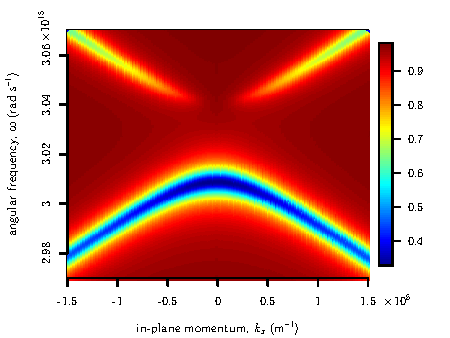
\includegraphics[]{figure-bandedgecoupling-band3}\label{fig:couplingbandedgesC}}
\end{center}
\caption[Sketches of different grating profiles determined by the relative phases of the $k_g$ and $2k_g$ components, and the resulting coupling of the light to the band-edges.]{Sketches of different grating profiles determined by the relative phases of the $k_g$ and $2k_g$ components (left), and the resulting coupling of the light to the band-edges, shown as modelled reflectivity plots (right). \label{fig:couplingbandedges}}
\end{figure}
For the first case, $\psi=0^\circ$, both band edges couple strongly to light, and are shown as a minimum in the reflectivity, forming two symmetric blue bands. For $\psi=+90^\circ$, only the upper frequency (higher energy) is coupled, while for $\psi=-90^\circ$, only the lower frequency band edge is coupled. 

The explanation for this phase dependent coupling is demonstrated in the figures of the grating profiles and components, also shown in figure \ref{fig:couplingbandedges}. The lower half space of each of these sketches shows the relative phase between the two grating components, and the upper half-space shows the resultant surface profile by addition of the $k_g$ and $2k_g$ components.
Firstly, by symmetry, the nodes and anti-nodes of a SPP standing wave on such a grating will occur at \textit{either} the peaks \textit{or} the troughs of the $2k_g$ component. Alternating nodes and anti-nodes at these points provide a SPP standing wave which satisfies the symmetry of the grating, and also has a wave vector equal to $(k_g-(-k_g))/2=k_g$ at normal incidence (which is half way between the $+k_g$ and $-k_g$ scattered SPPs). One SPP standing wave charge arrangement will require induced charge at the peaks of the $2k_g$ component, while the other solution will require the charge to accumulate at the troughs.

In order for light to couple to the SPP standing waves, the electric field vector must have a component normal to the surface by which the impinging field may induce surface charge and hence couple to the surface electron density oscillations. In figure \ref{fig:couplingbandedgesA}, the addition of the in-phase ($\psi=0^\circ$) $2k_g$ component leads to points for both the high energy (green dots) and low energy (blue dots) nodes and anti-nodes which lie on the grating profile where the gradient of the profile is not zero. Because the grating profile at these points is not flat, there is indeed a surface normal component which can match to the impinging electric field, and the result is that both the high energy and low energy solutions may couple to incident light. In the second case in figure \ref{fig:couplingbandedgesB}, where $\psi_2=+90^\circ$, the resulting surface profile only has a non-zero gradient for the high energy solution (green dots), while the position of the low-energy `hot-spots' (the $2k_g$ minima) occur at a flat region of the grating. Consequently, no coupling occurs for the lower-energy mode, and only the upper band is coupled, as seen in the reflectivity plot. Finally, for the $\psi_2=-90^\circ$ case in figure \ref{fig:couplingbandedgesC}, the resulting geometry provides a normal component of the surface to the electric field only at the blue dot locations, corresponding to an induced charge arrangement for the low-energy band. The high-energy arrangement points are located at the $2k_g$ component's maxima, and exist on flat regions of the grating geometry. The coupling of light in this case is then only to the lower-energy mode. 


\subsection{Polarisation Conversion}
Linearly polarised light incident on a grating may be converted to the orthogonal linear polarisation state in a process named `polarisation conversion'. Two mechanisms have been identified for this conversion using diffraction gratings; one is mediated by SPPs, and the other is due to the phase lag of the different reflected polarisation state reflections on deep gratings.

SPPs may mediate the polarisation conversion of incident light when the excited SPPs travel along the grating surface in a direction of broken symmetry \cite{Bryan-Brown1990,Depine2001,Elston1991,Inagaki:86}. For the monograting case, this is any azimuthal angle other than $\phi = 0^\circ$ or $90^\circ$. In such an orientation, both TM and TE polarised light provide a normal component of electric field to the grating surface and so may induce surface charge and resonantly drive SPPs. Since this is the case, it is clear that SPPs decaying back into propagating light may couple back out into either the TM or TE polarisation state, and so polarisation conversion is possible. For shallow gratings, the maximum polarisation conversion occurs at an azimuthal angle of $\phi=45^\circ$, where the coupling to SPPs with TM and TE polarised light is equal. For shallow gratings, the polarisation converted signal is proportional to $\sin^2 (2\phi)$, which is shown simply by the consideration of the the electric field components relative to the grating surface \cite{Bryan-Brown1990}. 
For bigratings, the same considerations hold true. A SPP can mediate polarisation conversion when travelling along an axis with no mirror symmetry, and cannot otherwise. For example, at $\phi=45^\circ$ on a square bigrating, no polarisation conversion is expected. 

The second method by which diffraction gratings may exhibit polarisation conversion is again due to broken symmetry between the two orthogonal polarisation states \cite{Watts1997a}. This process is not mediated by SPPs and may occur on sub-wavelength, non-diffracting gratings providing the grooves are sufficiently deep. Consider the simple case of a non-diffracting monograting, the electric field incident on the grating surface may be considered to decompose in two directions, one parallel to the grating grooves  ($E_\parallel$) and one perpendicular ($E_\perp$) to the grooves. Since $E_\parallel$ does not cut across the grating grooves, this field will reflect as if it were reflected from a planar surface at a position equal to the average plane of the grating. However, since $E_\perp$ cuts across the grating grooves, circulating fields may be produced in these grooves which alter the effective average plane of reflection for this field component. The difference in position of these `effective mirrors' produces a phase difference between the two components which serves to rotate the plane of polarisation, leading to polarisation conversion. The maximum polarisation conversion on such gratings occurs when the phase difference between the reflected $E_\parallel$ and $E_\perp$ is $180^\circ$, and so is a cyclic function with respect to the depth of the grating. This necessity for the field components to be $180^\circ$ out of phase requires the gratings to be reasonably deep. For a gold sinusoidal grating illuminated with $\lambda_0=632.8\:\nano\metre$ with a pitch of $300\:\nano\metre$ the maximum polarisation converted signal occurs at a groove depth of $\approx 180\:\nano\metre$ \cite{Watts1997a}.

